\documentclass[acmsmall,manuscript,screen,review]{acmart}

%%
%% \BibTeX command to typeset BibTeX logo in the docs
\AtBeginDocument{%
  \providecommand\BibTeX{{%
    Bib\TeX}}}

%% Rights management information.  This information is sent to you
%% when you complete the rights form.  These commands have SAMPLE
%% values in them; it is your responsibility as an author to replace
%% the commands and values with those provided to you when you
%% complete the rights form.
\setcopyright{acmcopyright}
\copyrightyear{2022}
\acmYear{2022}
\acmDOI{XXXXXXX.XXXXXXX}


%%
%% These commands are for a JOURNAL article.
\acmJournal{FAC}
\acmVolume{1}
\acmNumber{1}
\acmArticle{1}
\acmMonth{1}

%%
%% Submission ID.
%% Use this when submitting an article to a sponsored event. You'll
%% receive a unique submission ID from the organizers
%% of the event, and this ID should be used as the parameter to this command.
%%\acmSubmissionID{123-A56-BU3}

%%
%% For managing citations, it is recommended to use bibliography
%% files in BibTeX format.
%%
%% You can then either use BibTeX with the ACM-Reference-Format style,
%% or BibLaTeX with the acmnumeric or acmauthoryear sytles, that include
%% support for advanced citation of software artefact from the
%% biblatex-software package, also separately available on CTAN.
%%
%% Look at the sample-*-biblatex.tex files for templates showcasing
%% the biblatex styles.
%%

%%
%% The majority of ACM publications use numbered citations and
%% references.  The command \citestyle{authoryear} switches to the
%% "author year" style.
%%
%% If you are preparing content for an event
%% sponsored by ACM SIGGRAPH, you must use the "author year" style of
%% citations and references.
%% Uncommenting
%% the next command will enable that style.
%%\citestyle{acmauthoryear}

\newtheorem{definition}{Definition}
\newtheorem{remark}{Remark}

\usepackage{graphicx}
\usepackage{subfigure}
\usepackage{color}
\usepackage{url}
%\usepackage{algorithm}  
%\usepackage{algorithmic} 
\usepackage{multirow}
\usepackage{placeins}

\usepackage{amsfonts}
\usepackage{mathrsfs}
\usepackage{amsmath}
\usepackage[linesnumbered,ruled,noend]{algorithm2e}
\usepackage{graphicx}
\usepackage{multirow}
\usepackage{color}
\usepackage{url}
\usepackage{enumitem}
\usepackage{tcolorbox}
\usepackage{tikz}
\usepackage{array}
\usepackage{listings}
\usepackage{float}
% \usepackage[dvipsnames]{xcolor}
%\usepackage{subcaption}
%\renewcommand{\lstlistingname}{Figure}

\lstset{
    language=Java, 
    basicstyle=\ttfamily\small, 
%   breaklines=true, 
    morekeywords={final, true, null, private, false, ArrayList}, keywordstyle=\color{blue!60!black},
    morekeywords=[2]{void, Task, ActivityRecord, NeededUriGrants, boolean, int, TaskFragment, ActivityOptions, IVoiceInteractionSession, IVoiceInteractor, BalCode, Fragment}, keywordstyle=[2]\color{red!60!black},
    morekeywords=[3]{computeTargetTask, recycleTask, startActivityInner, getOrCreateRootTask, complyActivityFlags, executeOps, executePopOps, expandOps, getReusableTask, setNewTask, addOrReparentStartingActivity}, keywordstyle=[3]\color{darkgray},
    commentstyle=\itshape\color{teal}, 
    stringstyle=\bfseries\color{teal}, 
    columns=flexible,
    frame=single, 
    framesep=0.1em,
    xrightmargin=1pt,
    lineskip=-0.5ex
}

%%%%%%% increase the nesting depth
\usepackage{enumitem}
\setlistdepth{9}

\setlist[itemize,1]{label=$\bullet$}
\setlist[itemize,2]{label=$-$}
\setlist[itemize,3]{label=$\ast$}
\setlist[itemize,4]{label=$\cdot$}
\setlist[itemize,5]{label=$\diamond$}
\setlist[itemize,6]{label=$\circ$}
\setlist[itemize,7]{label=$\star$}
\setlist[itemize,8]{label=$\triangleright$}
\setlist[itemize,9]{label=$\square$}

\renewlist{itemize}{itemize}{9}
%%%%%%% increase the nesting depth


\definecolor{highlightcolor}{rgb}{0.9,0.9,0.9}

% correct bad hyphenation here
\hyphenation{op-tical net-works semi-conduc-tor}
\newcommand\Aa{{\mathcal{A} }}
\newcommand\Bb{{\mathcal{B} }}
\newcommand\Cc{{\mathcal{C} }}
\newcommand\Dd{{\mathbb{D} }}
\newcommand\Ee{{\mathcal{E} }}
\newcommand\Ff{{\mathcal{F} }}
\newcommand\Gg{{\mathcal{G} }}
\newcommand\Jj{{\mathcal{J}}}
\newcommand\Ll{{\mathcal{L}}}
\newcommand\Mm{{\mathcal{M} }}
\newcommand\Nn{{\mathbb{N} }}
\newcommand\Oo{{\mathcal{O} }}
\newcommand\Pp{{\mathcal{P} }}
\newcommand\Ss{{\mathcal{S} }}
\newcommand\Tt{{\mathcal{T} }}
\newcommand\transet{{\mathscr{T} }}
%\def\Ii{{\mathbb{Z} }}
\newcommand\Rr{{\mathcal{R} }}
\newcommand\Vv{{\mathcal{V}}}
\newcommand\Zz{{\mathcal{Z} }}

\newcommand\PosNat{{\mathbb{N}_{> 0} }}

\newcommand\frag{{\sf Frg}}
\newcommand\act{{\sf Act}}
\newcommand\aft{{\sf Aft}}
\newcommand\lmd{{\sf Lmd}}
\newcommand\atr{{\sf Atr}}

%\newcommand\vgr{{\sf Vgr}}
\newcommand\vgr{{\sf Ctn}}
\newcommand\cid{{\sf CID}}

\newcommand\tact{{\sf Top}}
\newcommand\bact{{\sf Btm}}
\newcommand\btmact{{\sf BtmAct}}
\newcommand\ract{ \bact}
\newcommand\standard{{\sf STD}}
\newcommand\singletop{{\sf STP}}
\newcommand\singletask{{\sf STK}}
\newcommand\singleinstance{{\sf SIT}}
\newcommand\STD{{\sf STD}}
\newcommand\STK{{\sf STK}}
\newcommand\STP{{\sf STP}}
\newcommand\SIT{{\sf SIT}}
\newcommand\opstack{{\sf TS}}
\newcommand\nopstack{{\sf NTS}}
\newcommand\tfrag{{\sf TopFrg}}

\newcommand\weight{{\mathsf{weight} }}


\newcommand\ops{\mathcal{T}}
\newcommand\cops{\mathcal{CT}}

\newcommand\actinstr{{\mathsf{ActInst} }}
\newcommand\fraginstr{{\mathsf{FrgInst} }}

\newcommand\ntkflag{{\sf NTK}}
\newcommand\ctpflag{{\sf CTP}}
\newcommand\stpflag{{\sf STP}}
\newcommand\ctkflag{{\sf CTK}}
\newcommand\mtkflag{{\sf MTK}}
\newcommand\rtfflag{{\sf RTF}}
\newcommand\tohflag{{\sf TOH}}
\newcommand\ndmflag{{\sf NDM}}
\newcommand\pitflag{{\sf PIT}}
\newcommand\rtnflag{{\sf RTN}}
\newcommand\nohflag{{\sf NOH}}
\newcommand{\LTK}{\mathsf{LTK}}
\newcommand{\ADD}{\mathsf{ADD}}
\newcommand{\CLR}{\mathsf{CLR}}
\newcommand{\REM}{\mathsf{REM}}
\newcommand{\REP}{\mathsf{REP}}
\newcommand{\HIDE}{\mathsf{HIDE}}
\newcommand{\SHOW}{\mathsf{SHOW}}

\newcommand\mainflag{{\sf MAIN}}

\newcommand{\AFSM}{\textsf{AFSM}}
\newcommand{\AMASS}{\textsf{AMASS}}
\newcommand{\AOAMASS}{\textsf{AMASS}_{ACT}}
\newcommand{\FOAMASS}{\textsf{AMASS}_{FRG}}
\newcommand{\LMAOAMASS}{\textsf{AMASS}_{ACT,LM}}
\newcommand{\IFAOAMASS}{\textsf{AMASS}_{ACT,IF}}

\newcommand{\AMSM}{\textsf{AMSM}}

\newcommand{\addr}{\symbol{64}}

\newcommand\actsig{{\sf Sig}}

\newcommand\mainact{{\sf mainAct}}

\newcommand\true{{\mathsf{true} }}

\newcommand\false{{\mathsf{false} }}

\newcommand\instr{{\mathsf{Inst} }}

\newcommand\back{{\mathsf{back} }}

\newcommand\startactivity{{\mathsf{start} }}

\newcommand\finishstart{{\mathsf{finishStart} }}

\newcommand\switchto{{\mathsf{switchTo} }}

\newcommand\tasks{{\mathsf{Tasks} }}
\newcommand\acts{{\mathsf{Acts} }}
\newcommand\task{{\mathsf{Task} }}


\newcommand\theapp{{\mathsf{ValApp} }}
\newcommand\dom{{\mathsf{dom} }}

\newcommand\range{{\mathsf{rng} }}

\newcommand\confs{{\mathsf{Confs} }}

\newcommand\reparent{{\mathsf{Rpt} }}

\newcommand\benign{{\mathsf{bgn} }}

\newcommand\malicious{{\mathsf{mlc} }}

\newcommand\conf{{\mathsf{Conf} }}

\newcommand\pre{{\mathsf{pre} }}

\newcommand\post{{\mathsf{post} }}

\newcommand\abs{{\mathsf{Abs} }}

\newcommand\sfx{{\mathsf{Sfx} }}

\newcommand\jump{\mathsf{Jump}}



\newcommand{\hide}[1]{}

\newcommand\natnum{{\mathbb{N} }}
\newcommand\intnum{{\mathbb{Z} }}


\newcommand{\ifz}{{\sf ifz}}
\newcommand{\inc}{{\sf inc}}
\newcommand{\dec}{{\sf dec}}


\newcommand\pop{{\sf pop}}
%\newcommand\mtrans{{\sf MTrans}}
\newcommand\reach{{\sf Reach}}

\newcommand{\enc}{{\sf enc}}

\newcommand{\art}{{\sf Art}}

\newcommand{\eact}{{\sf EAct}}
\newcommand{\cact}{{\sf CAct}}

\newcommand{\sat}{{\sf Sat}}

\newcommand{\sub}{{\sf Sub}}


\newcommand{\myvec}[1]{{\footnotesize{\begin{bmatrix}#1\end{bmatrix}}}}

\newcommand{\emptybackstack}{\triangleright}
\newcommand{\noaction}{\square}


\newcommand\flagset{\mathcal{F}}
\newcommand\bool{\mathscr{B}}

\newcommand\realact{\mathsf{RealAct}}
\newcommand\toptsk{\mathsf{TopTsk}}
\newcommand\topact{\mathsf{TopAct}}
\newcommand\preact{\mathsf{PreAct}}
\newcommand\topfrag{\mathsf{TopFrag}}
\newcommand\push{\mathsf{Push}}
\newcommand\mvacttop{\mathsf{MvAct2Top}}
\newcommand\clrtop{\mathsf{ClrTop}}
\newcommand\clrtsk{\mathsf{ClrTsk}}
\newcommand\mvtsktop{\mathsf{MvTsk2Top}}
\newcommand\rmtsk{\mathsf{RmTsk}}
\newcommand\rmact{\mathsf{RmAct}}
\newcommand\rptoptsk{\mathsf{RpTopTsk}}
\newcommand\newtsk{\mathsf{NewTsk}}
\newcommand\ismultsk{\mathsf{HasMulTsk}}
\newcommand\hastartsk{\mathsf{HasNMainMulTsk}}
\newcommand\gettsk{\mathsf{GetTsk}}
\newcommand\getrealtsk{\mathsf{GetRealTsk}}
\newcommand\getsittsk{\mathsf{GetSitTsk}}
\newcommand\getmultsk{\mathsf{GetNMainMulTsk}}
\newcommand\getmaintsk{\mathsf{GetMulTsk4A0}}
\newcommand\getnulltsk{\mathsf{GetEmpAftTsk}}
\newcommand\getfrag{\mathsf{GetFrag}}
%\newcommand\updateviews{\mathsf{UpdateViews}}
\newcommand\updateviews{\mathsf{UpdateCtns}}
%\newcommand\getview{\mathsf{GetViews}}
\newcommand\form{\mathsf{Form}}

\newcommand\getCons{\mathsf{GetCons}}
\newcommand\devideCons{\mathsf{DevideCons}}
\newcommand\norm{\mathsf{Norm}}
\newcommand\getFrags{\mathsf{GetFrags}}
\newcommand\nuxmv{nuXmv}

%\newcommand\getopt{\mathsf{GetOpts}}
\newcommand\concaction{\mathsf{Concretize}}


\newcommand\isswitchingtsk{\mathsf{IsSwitchingTsk}}
\newcommand\sourceact{\mathsf{SourceAct}}
\newcommand\targetact{\mathsf{TargetAct}}
\newcommand\srealact{\mathsf{SourceRealAct}}
\newcommand\trealact{\mathsf{TargetRealAct}}
\newcommand\reachmap{\mathsf{ReachMap}}
\newcommand\reachmaps{\mathsf{ReachMaps}}
\newcommand\exmap{\mathsf{ExMap}}
\newcommand\exmaps{\mathsf{ExMaps}}
\newcommand\tskmap{\mathsf{TaskMap}}
\newcommand\export{\mathsf{ExPorts}}
\newcommand\enport{\mathsf{EnPorts}}

%%%%%%%%%%%%%hcancel and mhcancel
\newcommand{\hcancel}[1]{%
	\tikz[baseline=(tocancel.base)]{
		\node[inner sep=0pt,outer sep=0pt] (tocancel) {#1};
		\draw[black] (tocancel.south east) -- (tocancel.north west);
	}%
}%
%\newcommand{\mhcancel}[1]{\text{\hcancel{\ensuremath{#1}}}}

%%%%%%%%%%%%%circled and mcircled
\usetikzlibrary{shapes,snakes}
\newcommand\rectangled[1]{\tikz[baseline=(torect.base)]{
		\node[shape = rectangle, draw, inner sep=0pt, outer sep = 0pt] (torect) {#1}
	}
}
\newcommand{\mrectangled}[1]{\text{\rectangled{\ensuremath{#1}}}}

\newcommand{\mhcancel}[1]{\mrectangled{#1}}


\newcommand{\footlabel}[2]{%
	\addtocounter{footnote}{1}%
	\footnotetext[\thefootnote]{%
		\addtocounter{footnote}{-1}%
		\refstepcounter{footnote}\label{#1}%
		#2%
	}%
	$^{\ref{#1}}$%
}

%\newcommand{\footref}[1]{%
%	$^{\ref{#1}}$%
%}


\newcommand{\container}{container}
\newcommand{\tabincell}[2]{\begin{tabular}{@{}#1@{}}#2\end{tabular}}



\newcommand\shortlong[2]{#2}
%\newcommand\shortlong[2]{#1}

\newif\ifdraft\drafttrue
%\newif\ifdraft\draftfalse
\ifdraft
\newcommand{\jinlong}[1]{\color{red} {JL: #1 :LJ} \color{black}}
\newcommand{\zhilin}[1]{\color{blue} {ZL: #1 :LZ} \color{black}}
\newcommand{\tl}[1]{\color{magenta} {TL: #1 :LT} \color{black}}
% \newcommand{\revision}[1]{\color{red} {JL: #1 :LJ} \color{black}}
\newcommand{\revision}[1]{\textcolor{red}{#1}}
\else
\newcommand{\jinlong}[1]{}
\newcommand{\zhilin}[1]{}
\newcommand{\tl}[1]{}
% \newcommand{\revision}[1]{}
\fi

\newcommand{\tool}{{\textsf TaskDroid}}

%%%%%%%%%%%%%%%%%%%%%%%%%%%%%%%%%%%%%%%%%%%%%%%%%%%%%%%%%%%%%%%%%%%%%%%%%%%%%%%%%%%%%

%%
%% end of the preamble, start of the body of the document source.
\begin{document}


%%
%% The "title" command has an optional parameter,
%% allowing the author to define a "short title" to be used in page headers.
\title{Formalization of Android Activity-Fragment Multitasking Mechanism and Static Analysis of Mobile Apps}

%%
%% The "author" command and its associated commands are used to define
%% the authors and their affiliations.
%% Of note is the shared affiliation of the first two authors, and the
%% "authornote" and "authornotemark" commands
%% used to denote shared contribution to the research.

\author{Jinlong He}
\affiliation{%
  \institution{State Key Laboratory of Computer Science, Institute of Software, Chinese Academy of Sciences}
  \streetaddress{No. 4 South 4th Street, Zhongguancun, Haidian District}
  \city{Beijing}
  \country{China}}
\affiliation{%
  \institution{School of Computer Science and Technology, University of Chinese Academy of Sciences}
  \streetaddress{No.19(A) Yuquan Road, Shijingshan District}
  \city{Beijing}
  \country{China}}  
\email{hejl@ios.ac.cn}

\author{Zhilin Wu}
\affiliation{%
  \institution{State Key Laboratory of Computer Science, Institute of Software, Chinese Academy of Sciences}
  \streetaddress{No. 4 South 4th Street, Zhongguancun, Haidian District}
  \city{Beijing}
  \country{China}}
\affiliation{%
  \institution{School of Computer Science and Technology, University of Chinese Academy of Sciences}
  \streetaddress{No.19(A) Yuquan Road, Shijingshan District}
  \city{Beijing}
  \country{China}}  

\author{Taolue Chen}
\affiliation{%
 \institution{School of Computing and Mathematical Sciences, Birkbeck, University of London}
 \streetaddress{Malet Street, Bloomsbury}
 \city{London}
 \country{UK}}

%%
%% By default, the full list of authors will be used in the page
%% headers. Often, this list is too long, and will overlap
%% other information printed in the page headers. This command allows
%% the author to define a more concise list
%% of authors' names for this purpose.
\renewcommand{\shortauthors}{He et al.}

%%
%% The abstract is a short summary of the work to be presented in the
%% article.
\begin{abstract}
The multitasking mechanism between activities and fragments plays a fundamental role in the Android operating system, which involves a wide range of
features, including launch modes, intent flags, task affinities, and structured activities containing fragments. All of them
are being widely used in Android apps, both open-source and commercial ones. In this paper, we present a formal
semantics of the Android multitasking mechanism  between activities and fragments, which accommodates all the important features and gives insofar
the most comprehensive and accurate formalization. In particular,
our semantics is formulated based on multi-stack systems, and
fully captures the behavior of task stacks and activity stacks
regarding fragments. Based on the semantics, we provide
new static analysis algorithms, which are both multi-stack-aware and 
fragment-sensitive, thus achieve more precise static analysis for Android apps.
We validate our approach by extensive experiments on both
open-source and commercial Android apps. The results highlight
the benefits of the considering the semantics of the
multitasking mechanism between activities and fragments in static analysis, and
confirm the efficacy of our approach.
\end{abstract}

%%
%% The code below is generated by the tool at http://dl.acm.org/ccs.cfm.
%% Please copy and paste the code instead of the example below.
%%
\begin{CCSXML}
<ccs2012>
<concept>
<concept_id>10003752.10010124.10010131.10010134</concept_id>
<concept_desc>Theory of computation~Operational semantics</concept_desc>
<concept_significance>500</concept_significance>
</concept>
<concept>
<concept_id>10011007.10011074.10011099.10011692</concept_id>
<concept_desc>Software and its engineering~Formal software verification</concept_desc>
<concept_significance>500</concept_significance>
</concept>
</ccs2012>
\end{CCSXML}

\ccsdesc[500]{Theory of computation~Operational semantics}
\ccsdesc[500]{Software and its engineering~Formal software verification}

%%
%% Keywords. The author(s) should pick words that accurately describe
%% the work being presented. Separate the keywords with commas.
\keywords{Android multitasking mechanism, activities and fragments, formal semantics, stack unboundedness, static analysis}

\received{20 February 2007}
\received[revised]{12 March 2009}
\received[accepted]{5 June 2009}

%%
%% This command processes the author and affiliation and title
%% information and builds the first part of the formatted document.
\maketitle

%%%%%%%%%%%%%%%%%%%%%%%%%%%%%%%%%%%%%%%%%%%%%%%%%%%%%%%%%%%%%%%%%%%%%%%%%%%%%%%%%%%%%%%%%%%%%%%%%%

\section{Introduction}\label{sec:introduction}
%!TEX root = main.tex

Android, a mobile operating system developed by Google, serves over 2 billion monthly active users and occupies over $80\%$ of the share of the global mobile operating system market.\footnote{\url{https://expandedramblings.com/index.php/android-statistics/}}
The Google Play App store, Google's official pre-installed app store on Android devices, has supplied 2 million apps since 2016.\footnote{\url{https://www.statista.com/statistics/266210/number-of-available-applications-in-the-google-play-store/}} 

Multitasking mechanism between activities and fragments plays a fundamental role in the Android operating system. Mobile apps provide diverse functionalities with seamless user experience by interacting with other apps.
For example, the Gallery app utilizes the Email app to send pictures rather than implements its own email
functionality \footnote{\url{https://play.google.com/store/apps/details?id=com.google.android.apps.photosgo&hl=en_US}}. These features require the support of frequent switch between apps. Moreover, Android provides a ``back" button by which users can easily switch between apps. 
%While users may think that a single app manages pictures and sends emails, the actual implementation consists of two independent apps using inter-app communication.

To facilitate smooth app switching and history recalling, Android introduces a last-in-first-out data structure, generally referred to as \emph{back stack}, to store users’ histories.
Technically speaking, the back stack exhibits a three-tier nested structure. At the highest layer there is a stack of tasks where each task can be considered as a stack of activities (the middle layer), and each activity may contain fragment stacks (the lowest layer). In other words, the back stack exhibits a hierarchy of task stack, activity stack and fragment stack. From the functionality perspective, a task %, as a logical notion, 
is a collection of activities that users interact with when performing a certain job (e.g., view email); an activity is a type of app components, which provides a graphical user interface (GUI) on screen and serves the entry point of the interaction with users. To facilitate GUI reuse, an activity may be further divided into fragments. 
A fragment defines and manages its own layout, has its own lifecycle, and can handle its own input events. It cannot live on its own, i.e., must be hosted by an activity. 
%A fragment represents reusable portions of android app's user interface in the activity.

Activities are a central concept in the Android multitasking mechanism. In particular, 
the evolution of %the contents of 
the back stack depends on various attributes of activities, including launch modes and task affinities, as well as the intent flags when starting activities. 
Moreover, the updates of the fragment containers in activities are controlled by fragment transactions (cf.\ Section~\ref{sec:amm} for more details).

%%%%%%%%%%%%%%%%%%%%%%%%%%%%%%%%%%%%%%%%%%% relocate to related work %%%%%%%%%%%%%%%%%%%%%%%%%%%

%In light of its central role in %testing and 
%analyzing Android apps, the multitasking mechanism has been considered in literature. To the best of our knowledge, this line of work was initiated in \cite{AN13}, where the concept of activity transition graphs (ATG) was proposed. ATGs are directed graphs where nodes are activities and edges describe the relationships that an activity can start the other. ATGs can be used for generating traces in GUI testing. An extension of ATGs, i.e., window transition graphs (WTGs) were proposed in \cite{YZWWYR15}. In WTGs, windows are assumed to be stored in one stack; nodes are windows that include not only activities, but also menus and dialogs; transitions represent a sequence of push/pop operations associated with sequences of callbacks. 
%ATGs were also extended in \cite{YWYZ17}, giving rise to the LATTE model, a finite-state machine model which stores the activities in a bounded-height stack as well as some state information transferred across activities. Moreover, in \cite{ZSX18}, activities were assumed to be stored into a stack and its contents were used as contexts for GUI testing and pointer analysis. In \cite{LWX18}, a tool called TDroid was developed to utilize the syntactic pattens on the launch modes, intent flags, and task affinities to detect the app switching attacks.
% 
%
%All of the above work did not consider fragments which were addressed in \cite{CHGD18}, where activity fragment transition graphs (AFTG) were proposed and used for GUI testing. %AFTGs extend ATGs by taking fragments into consideration.
%	%
%Furthermore, in \cite{LHR17,ChenHSWWY18,HCWWY19}, formal semantics for Android multitasking mechanism were proposed and used for the static analysis of Android apps.

%%%%%%%%%%%%%%%%%%%%%%%%%%%%%%%%%%%%%%%%%%% relocate to related work %%%%%%%%%%%%%%%%%%%%%%%%%%%
 

%, as a result of its importance in Android operating system. 
%We briefly survey the state-of-the-art in the sequel (which, nonetheless, does not aim to be complete.).
%
%\begin{itemize}
%\item This line of work was initialized In \cite{AN13}, where the concept of activity transition graphs (ATG) was proposed. ATGs are directed graphs where nodes are activities and edges describe the relationships that an activity can start the other. ATGs can be used for generating traces in GUI testing.
%%
%\item Then in \cite{YZWWYR15}, window transition graphs (WTGs) were proposed as an extension of ATGs. In WTGs, the windows are assumed to be stored in one stack and the nodes are windows that include not only activities, but also menus and dialogs, moreover, the transitions represent a sequence of push/pop operations and are associated with the sequences of callbacks. 
%%
%\item Later on, in \cite{YWYZ17}, the LATTE model was proposed, which is essentially a finite-state machine model that extends ATGs in the following sense: It stores the activities into a bounded-height stack as well some state information transferred across activities. 
%%
%\item Moreover, in \cite{ZSX18}, activities were assumed to be stored into a stack and its contents were used as contexts for GUI testing and pointer analysis.
%%
%\item In \cite{LWX18}, a tool called TDroid was proposed to detect the app switching attacks based on a syntactic patten approach.
%%%
%\item In \cite{CHGD18}, a concept of activity fragment transition graphs (AFTG) was proposed and used for GUI testing. AFTGs extend ATGs by taking fragments into consideration.
%%
%\item Furthermore, in \cite{LHR17,ChenHSWWY18,HCWWY19}, formal semantics for Android multitasking mechanism were proposed and used for the static analysis of Android apps.
%\end{itemize} 
% TaskDroid multi-stack semantics, static analysis, no fragments, no testing
%

%\paragraph*{Motivation.} 
%Although there have been aforementioned large body of work on back-stack-aware testing and analysis of Android apps,
%Despite 
In light of its central role in %testing and 
analyzing Android apps, the multitasking mechanism between activities and fragments has been considered in literature.
First, there have been decent work towards its formalization and we refer to readers to Section~\ref{sec:related} for some introduction. % of multitasking the progress, it is fair to say that 
%the understanding of Android multitasking mechanism and its application in Android app analysis and testing are still unsatisfactory. 
%in its infancy. 
%For the former, %there have not existed any 
However, the existing formal semantics is far from complete. A primary drawback is that the activities are treated as an atomic object therein, while the internal structures (e.g., fragments) were abstracted away. 
%This was indeed the case in the literature~\cite{LHR17,ChenHSWWY18,HCWWY19}. 
The understanding of semantics may play a significant role in carrying out semantics-aware analysis of the mobile app, which can capture more features of the Android platform and thus is more precise. In contrast, 
the state-of-the-art analysis largely applied a syntactic approach. The underlying stack semantics of the multitasking mechanism between activities and fragments is either ignored completely (\cite{AN13,LWX18,CHGD18}) or considered in a very much restricted form (e.g., single stack \cite{YZWWYR15}), or otherwise important features (e.g., task affinities or fragments) are skipped \cite{YZWWYR15,YWYZ17, ZSX18}.  
%\begin{itemize}
%\item in \cite{AN13}, ATGs were used syntactically and no semantics was given, 
%%
%\item in \cite{YZWWYR15}, WTGs adopted the single-stack semantics, but did not consider launch modes, intent flags, or fragments, 
%%
%\item in \cite{YWYZ17}, the LATTE model only considered launch modes and defined the single-stack semantics, ignored intent flags, task affinities, or fragments, 
%%
%\item in \cite{ZSX18},  only launch modes were considered, but intent flags, task affinities, and fragments were ignored, 
%%
%\item in \cite{LWX18}: a pattern-based approach was used and semantics were ignored, 
%%
%\item in \cite{CHGD18}, a syntactic approach was used and semantics were ignored, although both activities and fragments were both covered,
%%
%\item in \cite{LHR17,ChenHSWWY18,HCWWY19}, the multi-stack semantics were defined, but fragments were ignored, moreover, the semantics were not used for GUI testing.
%%
%\end{itemize}
%

The status quo is clearly unsatisfying. 
Indeed, all the multitasking features, including task affinities and fragments, are widely used in Android apps, especially the commercial ones. A small-scale survey on the 3,000 most downloaded commercial Android apps in Google play shows that almost all apps use launch modes and intent flags, about $10\%$ of the apps use non-default task affinities, and  about $50\%$ of the apps involve fragments. 
We address these shortcomings in the current paper. %This motivates the following research question: 
%
%\hl{
%Can a formal semantics of Android multitasking mechanism be defined to cover all important features (in particular, task affinities and fragments) and used to enhance the testing coverage and analysis precision of Android apps ?
%}

%%%%%%%%%%%%%%%%%%%%%%%%%%%%%%%%%%%%%%%%%%%%%%%%%%%%%%%%%%%%%%%%%%%%%%%%%%%%%%%%
\medskip
\noindent\emph{Main contributions.} In this paper, we make the following contributions. %aiming at resolving the research question, we make the following contributions: 
\begin{itemize}
\item We introduce a new model, Android multitasking stack machine (\AMASS), to define the formal semantics of the multitasking mechanism between activities and fragments. {\AMASS} covers all the important multitasking features (e.g., task affinities and fragments) and provides, to the best \revision{of} our knowledge, insofar the most comprehensive formal account of the Android multitasking mechanism between activities and fragments. Moreover, We validate the formal semantics of {\AMASS} models against the actual behavior of  Android apps by designing a special-purpose app and doing large-scale experiments with the app. 
%
\item We harness the semantics to design novel algorithms for static analysis of the abnormal behaviors of task unboundedness and fragment-container unboundedness. %, providing a higher testing coverage and analysis precision. 

\item We implement the algorithms into a static analysis tool called TaskDroid and experiment on a corpus of open source and commercial Android apps.  
%\tl{impressive figures?}. 
The results show that TaskDroid can detect the task/fragment-container unboundedness problems for open source and commercial Android apps and the unboundedness problems entail abnormal behaviors of Android apps, including black screen, app crash, and device reboot, owing to a fine-grained semantic modeling of Android multitasking mechanism between activities and fragments.  %the analysis precision. 
\end{itemize}

%%%%%%%%%%%%%%%%%%%%%%%%%%%%%%%%%%%%%%%%%%%%%%%%%%%%%%%%%%%%%%%%%%%%%%%%%%%%%%%
%Compared to \cite{HCWWY19}, this paper adds fragments, extends the analysis accordingly, moreover, the experiments are  more extensive. 

\subsection{Related work}\label{sec:related}
%!TEX root = main.tex

\noindent \textbf{Formalization of Android multitasking semantics.}
In light of its central role in  analyzing Android apps, the multitasking mechanism between activities and fragments has been considered in literature. To the best of our knowledge, this line of work was initiated in \cite{AN13}, where the concept of activity transition graphs (ATG) was proposed. ATGs are directed graphs where nodes are activities and edges describe the relationships that an activity can start the other. ATGs can be used for generating traces in GUI testing. An extension of ATGs, i.e., window transition graphs (WTGs) were proposed in \cite{YZWWYR15}. In WTGs, windows are assumed to be stored in one stack; nodes are windows that include not only activities, but also menus and dialogs; transitions represent a sequence of push/pop operations associated with sequences of callbacks. 
ATGs were also extended in \cite{YWYZ17}, giving rise to the LATTE model, a finite-state machine model which stores the activities in a bounded-height stack as well as some state information transferred across activities. Moreover, in \cite{ZSX18}, activities were assumed to be stored into a stack and its contents were used as contexts for GUI testing and pointer analysis. In \cite{LWX18}, a tool called TDroid was developed to utilize the syntactic pattens on the launch modes, intent flags, and task affinities to detect the app switching attacks.
All of the above work did not consider fragments which were addressed in \cite{CHGD18}, where activity fragment transition graphs (AFTG) were proposed and used for GUI testing. %AFTGs extend ATGs by taking fragments into consideration.
%
Furthermore, in \cite{LHR17,ChenHSWWY18,HCWWY19}, formal semantics for Android multitasking mechanism were proposed.
% and used for the static analysis of Android apps.
%
%Despite the progress, it is fair to say that the understanding
%of Android multitasking mechanism and its application in
%Android app analysis and testing are still unsatisfactory. For
%the former, 

%The existing formal semantics is unfortunately far from complete.
One serious drawback of the current formalization is that the activities are treated as
an atomic object therein, while the internal structures (e.g.,
fragments) were abstracted away. In this paper, we provide the first complete formal account 
of the operational semantics, differentiating different versions of Android, and carry out validation ensuring its conformance to the actual behavior.  

%This was indeed the case
%in [Chen et al. 2018b; He et al. 2019; Lee et al. 2017]. 

%\medskip
\noindent\textbf{Static analysis. }
%
%Static analysis exploits techniques that parse program source code or bytecode, often traversing program paths to check some program properties. 
Static analysis approaches have been applied to Android apps, where typical tasks include  %proposed for different tasks, including for 
assessing the security of Android apps, detecting app clones, automating test cases generation, or %for 
uncovering non-functional issues related to performance or energy \cite{LiBPRBOKT17}. There is a large body of work where in general the analysis techniques are still those which have been thoroughly considered in the static analysis of programs, e.g., control-flow analysis, data-flow analysis, and point-to analysis, but  are adapted to Android apps. 


A specific purpose of static analysis which is the closest to this paper is to reveal security vulnerabilities, many of which are related to the ICC mechanism and its potential misuses such as component hijacking. For instance,  \cite{LuLWLJ12} applied reachability analysis on customized system dependence graphs to detect component hijacking vulnerabilities, and \cite{OcteauMJBBKT13, OcteauLDJM15} implemented the detection of 
inter-component vulnerabilities. 
%(i.e., gain unauthorized access to protected or private resources through exported components in vulnerable apps) 
%or intent injection. %(i.e., manipulate user input data to execute code through it). 
%For example, CHEX [8] detects potential component hijacking- based flows through reachability analysis on customized system dependence graphs. Epicc [9] and IC3 [39] are tools that imple- ment static analysis techniques for implementing detection sce- narios of inter-component vulnerabilities. Based on these studies, PCLeaks [38] goes one step further by performing sensitive data- flow analysis on top of component vulnerabilities, enabling it to not only know what is the issue but also to know what sensi- tive data will leak through that issue. Similarly to PCLeaks, Con- tentScope [40] detects sensitive data leaks focusing on Content Provider-based vulnerabilities in Android apps.
We refer to \cite{LiBPRBOKT17} for a systematic literature review for the static analysis of Android apps.

In terms of static analysis  with respect to the multitasking mechanism between activities and fragments, 
the state-of-the-art analysis largely
applied a syntactic approach. The underlying stack semantics of the multitasking mechanism  between activities and fragments is either ignored completely (\cite{AN13,LWX18,CHGD18}) or considered in a restricted form (e.g., single stack \cite{YZWWYR15}), or otherwise important features (e.g., task affinities or fragments) are skipped \cite{YZWWYR15,YWYZ17, ZSX18}.  

\cite{LHR17}  develops a static analysis tool based on the operational semantics formalized therein, which can analyze  Android apps.  The tool extracts the necessary information (e.g., activity, intent flag)  and
%produces a report of possible activity injections. Using the
%activity information, intent data, and the activity activation
%semantics, it 
analyzes possible activity injection cases
to detect activity injection attacks. We are however not aware of other formal approaches towards analysis of Android apps accounting for the multitasking mechanism between activities and fragments similar to what we present in the current paper. 

%From a given Android apk archive, Activity Info. Extractor
%builds information about the activities in the app; it disassembles the resource files of the app using apktool [15] and
%extracts launchMode and taskAffinity of the activities
%from the AndroidManifest.xml file. Also, CHA CallGraph
%Builder takes the apk and constructs its call graph via Class
%Hierarchy Analysis (CHA) [16], which is often less precise
%than pointer analysis but much faster, since it analyzes only
%types rather than values. Then, Intent Analyzer extracts intent
%data that activate activities from the call graph. The intent
%data contain the target activity names of the intent and the
%set of intent flags added to the intent. Finally, Activity Injection
%Detector takes the activity information with intent data, and
%produces a report of possible activity injections. Using the
%activity information, intent data, and the activity activation
%semantics, it analyzes possible activity injection cases
%to detect activity injection attacks.

%\zhilin{More related work should be added} \tl{do we have more related work?}
 
%%%%%%%%%%%%%%%%%%%%%%%%%%%%%%%%%%%%%%%%%%%%%%%%%%%%%%%%%%%%%%%%%%%%%%%%%%%%%%%%
\medskip
 
\noindent\emph{Structure.} The rest of the paper is organized as follows. 
Section~\ref{sec:amm} gives an informal introduction to Android multitasking mechanism between activities and fragments. 
Section~\ref{sec-motiv-exmp} motivates this paper with two open-source apps from F-Droid. 
Section~\ref{sec:amass} introduces the {\AMASS} model and formalization of the multitasking mechanism  between activities and fragments. Section~\ref{sec:apk2amass} shows how to extract {\AMASS} models out of Android APK files. Section~\ref{sec:amass2fsm} describes how to encode the semantics of the {\AMASS} models into the reachability problem of finite state machines  that can be tackled by the symbolic model checker nuXmv, if the stack heights are assumed to be bounded by a constant. Section~\ref{sec:validation} is devoted to the validation of the formal semantics of {\AMASS} models against the actual behaviors of Android apps. 
Section~\ref{sec:static} presents the static analysis algorithms for the task/fragment-container unboundedness problems. 
Section~\ref{sec:eva} describes the implementation of the static analysis tool, TaskDroid, the benchmarks, and the experiments for the evaluation of TaskDroid. %The related work is discussed in Section~\ref{sec:related}.
The paper is concluded in Section~\ref{sec:conc}. 

\medskip

A preliminary version of this paper has appeared in the proceedings of APLAS 2019 \cite{HCWWY19}. This paper extends the APLAS paper in the following five aspects: (i) Fragments, a crucial feature of Android multitasking which was ignored in \cite{HCWWY19}, is fully addressed in the current paper, including the formal semantics and static analysis. (ii) The semantics of the multitasking mechanism between activities and fragments for Android 6.0-13.0 are defined in this paper, while only the semantics for Android 7.0 and 8.0 were defined in \cite{HCWWY19}. \revision{(iii) Compared to the semantics validation in~\cite{HCWWY19}, the semantics validation in this paper is extended in the following two ways: the relevant parts of the source code of Android OS are audited and 20 opens-source F-Droid apps are included to validate the semantics empirically, in addition to an app that is specially designed for the empirical validation.} (iv) The models are extracted both statically and dynamically in this paper, while only static model extraction was used in \cite{HCWWY19}. (v) The experiments are considerably more thoroughly done with, in particular, more benchmarks.
 


%\section{Related Work} \label{sec:related}
%%!TEX root = main.tex

\noindent \textbf{Formalization of Android multitasking semantics.}
In light of its central role in  analyzing Android apps, the multitasking mechanism between activities and fragments has been considered in literature. To the best of our knowledge, this line of work was initiated in \cite{AN13}, where the concept of activity transition graphs (ATG) was proposed. ATGs are directed graphs where nodes are activities and edges describe the relationships that an activity can start the other. ATGs can be used for generating traces in GUI testing. An extension of ATGs, i.e., window transition graphs (WTGs) were proposed in \cite{YZWWYR15}. In WTGs, windows are assumed to be stored in one stack; nodes are windows that include not only activities, but also menus and dialogs; transitions represent a sequence of push/pop operations associated with sequences of callbacks. 
ATGs were also extended in \cite{YWYZ17}, giving rise to the LATTE model, a finite-state machine model which stores the activities in a bounded-height stack as well as some state information transferred across activities. Moreover, in \cite{ZSX18}, activities were assumed to be stored into a stack and its contents were used as contexts for GUI testing and pointer analysis. In \cite{LWX18}, a tool called TDroid was developed to utilize the syntactic pattens on the launch modes, intent flags, and task affinities to detect the app switching attacks.
All of the above work did not consider fragments which were addressed in \cite{CHGD18}, where activity fragment transition graphs (AFTG) were proposed and used for GUI testing. %AFTGs extend ATGs by taking fragments into consideration.
%
Furthermore, in \cite{LHR17,ChenHSWWY18,HCWWY19}, formal semantics for Android multitasking mechanism were proposed.
% and used for the static analysis of Android apps.
%
%Despite the progress, it is fair to say that the understanding
%of Android multitasking mechanism and its application in
%Android app analysis and testing are still unsatisfactory. For
%the former, 

%The existing formal semantics is unfortunately far from complete.
One serious drawback of the current formalization is that the activities are treated as
an atomic object therein, while the internal structures (e.g.,
fragments) were abstracted away. In this paper, we provide the first complete formal account 
of the operational semantics, differentiating different versions of Android, and carry out validation ensuring its conformance to the actual behavior.  

%This was indeed the case
%in [Chen et al. 2018b; He et al. 2019; Lee et al. 2017]. 

%\medskip
\noindent\textbf{Static analysis. }
%
%Static analysis exploits techniques that parse program source code or bytecode, often traversing program paths to check some program properties. 
Static analysis approaches have been applied to Android apps, where typical tasks include  %proposed for different tasks, including for 
assessing the security of Android apps, detecting app clones, automating test cases generation, or %for 
uncovering non-functional issues related to performance or energy \cite{LiBPRBOKT17}. There is a large body of work where in general the analysis techniques are still those which have been thoroughly considered in the static analysis of programs, e.g., control-flow analysis, data-flow analysis, and point-to analysis, but  are adapted to Android apps. 


A specific purpose of static analysis which is the closest to this paper is to reveal security vulnerabilities, many of which are related to the ICC mechanism and its potential misuses such as component hijacking. For instance,  \cite{LuLWLJ12} applied reachability analysis on customized system dependence graphs to detect component hijacking vulnerabilities, and \cite{OcteauMJBBKT13, OcteauLDJM15} implemented the detection of 
inter-component vulnerabilities. 
%(i.e., gain unauthorized access to protected or private resources through exported components in vulnerable apps) 
%or intent injection. %(i.e., manipulate user input data to execute code through it). 
%For example, CHEX [8] detects potential component hijacking- based flows through reachability analysis on customized system dependence graphs. Epicc [9] and IC3 [39] are tools that imple- ment static analysis techniques for implementing detection sce- narios of inter-component vulnerabilities. Based on these studies, PCLeaks [38] goes one step further by performing sensitive data- flow analysis on top of component vulnerabilities, enabling it to not only know what is the issue but also to know what sensi- tive data will leak through that issue. Similarly to PCLeaks, Con- tentScope [40] detects sensitive data leaks focusing on Content Provider-based vulnerabilities in Android apps.
We refer to \cite{LiBPRBOKT17} for a systematic literature review for the static analysis of Android apps.

In terms of static analysis  with respect to the multitasking mechanism between activities and fragments, 
the state-of-the-art analysis largely
applied a syntactic approach. The underlying stack semantics of the multitasking mechanism  between activities and fragments is either ignored completely (\cite{AN13,LWX18,CHGD18}) or considered in a restricted form (e.g., single stack \cite{YZWWYR15}), or otherwise important features (e.g., task affinities or fragments) are skipped \cite{YZWWYR15,YWYZ17, ZSX18}.  

\cite{LHR17}  develops a static analysis tool based on the operational semantics formalized therein, which can analyze  Android apps.  The tool extracts the necessary information (e.g., activity, intent flag)  and
%produces a report of possible activity injections. Using the
%activity information, intent data, and the activity activation
%semantics, it 
analyzes possible activity injection cases
to detect activity injection attacks. We are however not aware of other formal approaches towards analysis of Android apps accounting for the multitasking mechanism between activities and fragments similar to what we present in the current paper. 

%From a given Android apk archive, Activity Info. Extractor
%builds information about the activities in the app; it disassembles the resource files of the app using apktool [15] and
%extracts launchMode and taskAffinity of the activities
%from the AndroidManifest.xml file. Also, CHA CallGraph
%Builder takes the apk and constructs its call graph via Class
%Hierarchy Analysis (CHA) [16], which is often less precise
%than pointer analysis but much faster, since it analyzes only
%types rather than values. Then, Intent Analyzer extracts intent
%data that activate activities from the call graph. The intent
%data contain the target activity names of the intent and the
%set of intent flags added to the intent. Finally, Activity Injection
%Detector takes the activity information with intent data, and
%produces a report of possible activity injections. Using the
%activity information, intent data, and the activity activation
%semantics, it analyzes possible activity injection cases
%to detect activity injection attacks.

%\zhilin{More related work should be added} \tl{do we have more related work?}
 

\section{Android Multitasking Mechanism Between Activities and Fragments} \label{sec:amm}
%!TEX root = main.tex

%\subsection{Android multitasking mechanism}

In this section, we briefly review the core concepts regarding the android multitasking mechanism, i.e., activities and fragments, and the evolution of the back stack. 
 
\subsection{Activity, task and task stack}
For the purpose of this paper, an Android app can be considered as a collection of \emph{activities}. At any time, there is one activity displayed on the screen of the device. 
The activities are organized into tasks. 
A \emph{task} is a collection of activities %that users interact with when performing 
to carry out a certain job. The running activities within a task are managed as an \emph{activity stack} 
%\emph{back stack} % this has been changed on 14/11/21
following the order that an activity is opened. In the activity stack, there are two distinguished activities, i.e., the \emph{root activity} and \emph{top activity}, which are sitting at the bottom and top of the stack respectively. %Note that %the back stack evolves in a way that the role of apps is diminished, in the  sense that
%in Android, activities from different apps can stay in the same task, and activities from the same app can enter different tasks.

The Android system normally run multiple tasks which are organized as the \emph{task stack}. The top task is the \emph{foreground} task whiles others are \emph{background} tasks. %They are organized as a task stack.
% as well, which is %for managing the current foreground task and previous background tasks. 
%referred to as a \emph{task stack} \cite{LHR17} (aka. activity stack \cite{RZXWL15}). 
%where The foreground task, as expected, sits on the top of the task stack. 
%
When a task comes to the foreground, its top activity is displayed on the device screen. When an activity finishes, it is popped from the activity stack. If the activity stack is not empty, the new top activity is displayed on the screen. Otherwise, the task itself finishes in which case it is popped from the task stack.  
We mention that, the Home screen comes to the foreground when a user presses the Home button (in this case the task stack will be emptied) or when the task stack becomes empty. The task stack  is the central data structure for Android multi-tasking mechanism, and we are mostly interested in its evolution in response to activity activation. When an activity is started, there are three basic attributes which determine the resulting task stack: \emph{launch modes, task affinities}, and \emph{intent flags}. %Developers can specify how to activate target activities
%The task stack is the central data structure for the Android multi-tasking mechanism, and we are mostly interested in its evolution in response to activity activation. 

 All the activities of an app, as well as their launch modes and task affinities, are defined in the \emph{manifest file}  
 ({\sf AndroidManifest.xml}). Differently, intent flags are set by caller activities to declare how to activate target activities by calling startActivity() or startActivityForResult() with the intent flags as its arguments. The launch mode attribute  specifies one of four modes to launch an activity: standard, singleTop, singleTask, and singleInstance, with standard being the default. A standard or singleTop activity can be instantiated multiple times leading to duplicated activities in a task. In contrast, an activity with the singleTask or singleInstance launch mode should be instantiated only once. Furthermore, an activity with the singleInstance launch mode is always the root activity of a task. While a singleTask activity
 can contain other standard or singleTop activities in its task, a singleInstance activity does not contain any other
 activities in its task. It is the only activity in its task; if it starts another activity, that activity is assigned to a different task. 
The task affinity attribute is of string data type and specifies to which task the activity prefers to belong. By default, all the activities from the same app have the same affinity, the package name of the app (i.e., all activities in the same app prefer to be in the same task). However, one can modify the default affinity of the activity. Android allows a great degree of flexibility: activities defined in different apps can share a task affinity whilst activities defined in the same app can be assigned with different task affinities.  

 
Android supports inter-component communication via \emph{intents}. An intent is an asynchronous message that activates activities. 
Android provides two types of intents, \emph{explicit} intents and \emph{implicit} intents. 
Explicit intents specify directly which activity to activate. Implicit intents, on the other hand, do not directly specify the activities which should be called, it only specifies actions to be performed. 
%A Uri can be used with the implicit intent to specify the data type.
For example, an implicit intent with the action ``ACTION\_VIEW'' and the data of \revision{the} URI ``http://www.google.com'' will cause a web browser to open a webpage. 
Android system searches for all activities which are registered for the specific action and the data type. If many activities are found then the user can select which activities to use.
In this paper, we restrict our attention to explicit intents since our focus is to understand the evolvement of the back stack when activities are started, and we do not attack the (another challenging) problem of resolving which activity should be started by implicit intents. 

Android provides 23 intent flags related to activities (see \cite{intentflags} for the detailed description of the intent flags). Intent flags are set by caller activities to declare how to activate target activities and are passed to startActivity() or startActivityForResult() as their arguments. 
%A detailed description of the meanings of these intent flags can be found in \url{https://developer.android.com/reference/android/content/Intent#flags}.
In this paper, among the 23 intent flags, we consider the following 10 ones, 
\begin{itemize}
	\item $\rm FLAG\_ACTIVITY\_NEW\_TASK$,
	\item $\rm FLAG\_ACTIVITY\_NEW\_DOCUMENT$,
	\item $\rm FLAG\_ACTIVITY\_MULTIPLE\_TASK$,
	\item $\rm FLAG\_ACTIVITY\_SINGLE\_TOP$,
	\item $\rm FLAG\_ACTIVITY\_REORDER\_TO\_FRONT$,
	\item $\rm FLAG\_ACTIVITY\_CLEAR\_TOP$,
	\item $\rm FLAG\_ACTIVITY\_CLEAR\_TASK$,
	\item $\rm FLAG\_ACTIVITY\_PREVIOUS\_IS\_TOP$,
	\item $\rm FLAG\_ACTIVITY\_NO\_HISTORY$,
	\item $\rm FLAG\_ACTIVITY\_TASK\_ON\_HOME$.
	%\item $FLAG\_ACTIVITY\_EXCLUDE\_FROM\_RECENTS$ (FAEFR),
	%	\item $\dots$.
\end{itemize}
\hide{
\begin{itemize}
	\item $\rm FLAG\_ACTIVITY\_NEW\_TASK$: this flag is set when the user wants to create a new task when starting an activity, 
	\item $\rm FLAG\_ACTIVITY\_NEW\_DOCUMENT$: this flag is set so that each instance of the activity (hosting a document) is put in a new task,
	\item $\rm FLAG\_ACTIVITY\_MULTIPLE\_TASK$: this flag is used to create a new task and launch an activity into it,
	\item $\rm FLAG\_ACTIVITY\_SINGLE\_TOP$: this flag is set so that the activity will not be launched if it is already running at the top of the history stack,
	\item $\rm FLAG\_ACTIVITY\_REORDER\_TO\_FRONT$: this flag will cause the launched activity to be brought to the front of its task if it is already running,
	\item $\rm FLAG\_ACTIVITY\_CLEAR\_TOP$: if this flag is set, then when the activity being launched is already running in the current task, instead of launching a new instance of that activity, all of the other activities on top of it will be closed,
	\item $\rm FLAG\_ACTIVITY\_CLEAR\_TASK$: if this flag is set, then any existing task that would be associated with the activity will be cleared before the activity is started,
	\item $\rm FLAG\_ACTIVITY\_PREVIOUS\_IS\_TOP$: if this flag is set, then the activity immediately below the foreground activity in the topmost task will be taken as the top activity for deciding whether a new instance of this activity should be created,
	\item $\rm FLAG\_ACTIVITY\_NO\_HISTORY$: if set, then the activity will be launched but not stored into the task stack, 
	\item $\rm FLAG\_ACTIVITY\_TASK\_ON\_HOME$: if this flag is set, then all the tasks, except the current home activity task, will be removed, and a new task is created to host this activity and pushed on top of the home activity task.
	%\item $FLAG\_ACTIVITY\_EXCLUDE\_FROM\_RECENTS$ (FAEFR),
	%	\item $\dots$.
\end{itemize}
}
The other 13 intent flags are ignored, for various reasons as shown in Table~\ref{tab-int-flag-ignore}.
\begin{table}[htbp]
\begin{center}
\small
    \begin{tabular}{|m{5.5cm}<{\centering}|m{8.5cm}<{\centering}|}
    \hline
    \textbf{Intent Flags} & \textbf{Reasons for being ignored in this paper}  \\
    \hline
	$\rm FLAG\_ACTIVITY\_REQUIRE\_DEFAULT$ & \multirow{3}*{Related to implicit intents, which we do not consider in this paper.}\\
	\cline{1-1}
	$\rm FLAG\_ACTIVITY\_REQUIRE\_NON\_BROWSER$ &\\
	\cline{1-1}
	$\rm FLAG\_ACTIVITY\_MATCH\_EXTERNAL$ & \\
    \hline
	$\rm FLAG\_ACTIVITY\_FORWARD\_RESULT$ & Used for transferring results between activities, which we do not consider in this paper.\\
    \hline
	$\rm FLAG\_ACTIVITY\_RETAIN\_IN\_RECENTS$  & \multirow{2}*{\shortstack{Related to the recent app list, which we do not consider it in this paper.}}\\
	\cline{1-1}
	$\rm FLAG\_ACTIVITY\_EXCLUDE\_FROM\_RECENTS$ &\\
    \hline
	$\rm FLAG\_ACTIVITY\_CLEAR\_WHEN\_TASK\_RESET$ & Deprecated from Android 5.0.\\
    \hline
	$\rm FLAG\_ACTIVITY\_BROUGHT\_TO\_FRONT$ & \multirow{2}*{Can only be set by Android operating system, not set by application code.}\\
	\cline{1-1}
	$\rm FLAG\_ACTIVITY\_LAUNCHED\_FROM\_HISTORY$ &\\
    \hline
	$\rm FLAG\_ACTIVITY\_NO\_USER\_ACTION$ & Related to the life-cycle of activities and we do not model the life-cycle of activities in this paper.\\
    \hline
	$\rm FLAG\_ACTIVITY\_NO\_ANIMATION$ &Used to show some animation when starting an activity and is not related to the evolvement of the back stack.\\
    \hline
	$\rm FLAG\_ACTIVITY\_LAUNCH\_ADJACENT$ & Related to the split-screen mode, which we do not consider in this paper.\\
    \hline
	$\rm FLAG\_ACTIVITY\_RESET\_TASK\_IF\_NEEDED$ & Related to the ``allowTaskReparenting'' attribute of activities, which we do not consider in this paper.\\
    \hline
    \end{tabular}
\end{center}
    \caption{Reasons for ignoring some intent flags in this paper}
    \label{tab-int-flag-ignore}
\end{table}

Besides launch modes, task affinities, and intent flags, there are some other factors that may also affect the behaviors of the task stack. 
When a caller activity calls startActivity() or startActivityForResult() to start a callee activity, the caller activity can also call the \emph{finish()} procedure so that when the callee activity is started, the caller activity is finished. 
Moreover, the \emph{real activity}\footnote{The name is inherited from the Android system.} of a task also matters. The real activity of a task is the activity that was pushed into the task as the bottom activity when the task was created. 
%Intuitively, $A_i$ is the activity which was pushed into the task---as the bottom activity---when the task $S_i$ was created. (Note that $A_i$ is not necessarily the current bottom activity of $S_i$.) 
If the real activity of a task is $B$ and the task is not the main task, then attempting to push an instance of $B$ to the task will not modify the task. 



\hide{
\begin{itemize}
\item The following three flags are related to implicit intents, which we do not consider in this paper:\\
 $\rm FLAG\_ACTIVITY\_REQUIRE\_DEFAULT$, $\rm FLAG\_ACTIVITY\_REQUIRE\_NON\_BROWSER$, \\
 $\rm FLAG\_ACTIVITY\_MATCH\_EXTERNAL$. 

\item The flag $\rm FLAG\_ACTIVITY\_FORWARD\_RESULT$ is for transferring results between activities, since we ignore results transferred between activities.

\item The two flags $\rm FLAG\_ACTIVITY\_RETAIN\_IN\_RECENTS$ and $\rm FLAG\_ACTIVITY\_EXCLUDE\_FROM\_RECENTS$ are ignored, since the recent app list is a data structure independent of the back stack and we do not consider it in this paper. 

\item The flag $\rm FLAG\_ACTIVITY\_CLEAR\_WHEN\_TASK\_RESET$ is deprecated from Android 5.0, thus ignored. 

\item The flags $\rm FLAG\_ACTIVITY\_BROUGHT\_TO\_FRONT$ and $\rm FLAG\_ACTIVITY\_LAUNCHED\_FROM\_HISTORY$ are ignored, since they can only be set by Android operating system, not set by application code. 

\item The flag $\rm FLAG\_ACTIVITY\_NO\_USER\_ACTION$ is related to the life-cycle of activities and we do not model the life-cycle of activities in this paper, thus ignored. 

\item The flag $\rm FLAG\_ACTIVITY\_NO\_ANIMATION$ is used to show some animation when starting an activity and is not related to the evolvement of the back stack, thus ignored. 

\item The flag $\rm FLAG\_ACTIVITY\_LAUNCH\_ADJACENT$ is related to the split-screen mode and we do not consider split-screen in this paper, thus ignored.  
%
\item The flag $\rm FLAG\_ACTIVITY\_RESET\_TASK\_IF\_NEEDED$ is related to the ``allowTaskReparenting'' attribute of activities, which we do not consider in this paper, thus this flag is ignored.  
\end{itemize}
}

 %%%%%%%%%%%%%%texts removed%%%%%%%%%%%%%%
 %%%%%%%%%%%%%%texts removed%%%%%%%%%%%%%%
  %%%%%%%%%%%%%%texts removed%%%%%%%%%%%%%%
 \hide{
 \revision{Among these 23 intent flags, we consider the following eleven, namely,}
\begin{itemize}
	\item $\rm FLAG\_ACTIVITY\_NEW\_TASK$ ($\ntkflag$),
	\item $\rm FLAG\_ACTIVITY\_NEW\_DOCUMENT$ ($\ndmflag$),
	\item $\rm FLAG\_ACTIVITY\_MULTIPLE\_TASK$ ($\mtkflag$),
	\item $\rm FLAG\_ACTIVITY\_SINGLE\_TOP$ ($\stpflag$),
	\item $\rm FLAG\_ACTIVITY\_REORDER\_TO\_FRONT$ ($\rtfflag$),
	\item $\rm FLAG\_ACTIVITY\_CLEAR\_TOP$ ($\ctpflag$),
	\item $\rm FLAG\_ACTIVITY\_CLEAR\_TASK$ ($\ctkflag$),
	\item $\rm FLAG\_ACTIVITY\_PREVIOUS\_IS\_TOP$ ($\pitflag$),
	\item $\rm FLAG\_ACTIVITY\_NO\_HISTORY$ ($\nohflag$),
	\item $\rm FLAG\_ACTIVITY\_RESET\_TASK\_IF\_NEEDED$ ($\rtnflag$),
	\item $\rm FLAG\_ACTIVITY\_TASK\_ON\_HOME$ ($\tohflag$).	
	%\item $FLAG\_ACTIVITY\_EXCLUDE\_FROM\_RECENTS$ (FAEFR),
	%	\item $\dots$.
\end{itemize}

\revision{The exclusion of the remaining 12 intent flags is justified as follows:}
\begin{itemize}
    \item $\rm FLAG\_ACTIVITY\_BROUGHT\_TO\_FRONT$: This flag is not normally set by application code, but set by system.
    \item $\rm FLAG\_ACTIVITY\_LAUNCHED\_FROM\_HISTORY$: This flag is not normally set by application code, but set by system.
%
    \item $\rm FLAG\_ACTIVITY\_CLEAR\_WHEN\_TASK\_RESET$: This flag was deprecated in API level 21 (Android 5.0).
%
    \item $\rm FLAG\_ACTIVITY\_LAUNCH\_ADJACENT$: This flag is only used for split-screen multi-window mode. The split screen is ignored at present, thus ignored.
%
    \item $\rm FLAG\_ACTIVITY\_RETAIN\_IN\_RECENTS$: If set, the new activity will remain in the recent task when it is finished. Recent task is different from back stack and not modeled, thus ignored.
%
    \item $\rm FLAG\_ACTIVITY\_EXCLUDE\_FROM\_RECENTS$: If set, the new activity is not kept in the recent task. Recent task is different from back stack and not modeled, thus ignored.
%
    \item $\rm FLAG\_ACTIVITY\_REQUIRE\_NON\_BROWSER$: If set, this flag will only launch the intent if it resolves to a result that is not a browser. If no such result exists, an ActivityNotFoundException will be thrown. In principle, we can support it if we know which activities belong to browsers. The current model extraction tool does not obtain such info, thus ignored.
%
    \item $\rm FLAG\_ACTIVITY\_REQUIRE\_DEFAULT$: If set, this flag will only launch the intent if it resolves to a single result. If no such result exists or if the system chooser would otherwise be displayed, an ActivityNotFoundException will be thrown. The implicit intent is not considered at present, thus ignored.
%
    \item $\rm FLAG\_ACTIVITY\_NO\_USER\_ACTION$: If set, this flag will prevent the normal Activity.onUserLeaveHint() callback from occurring on the current frontmost activity before it is paused as the newly-started activity is brought to the front. The lifecycle is not modeled at present, thus ignored.
%
    \item $\rm FLAG\_ACTIVITY\_NO\_ANIMATION$: If set, this flag will prevent the system from applying an activity transition animation to go to the next activity. The animation is ignored, since it does not affect back stack.
%
    \item $\rm FLAG\_ACTIVITY\_MATCH\_EXTERNAL$: If set, this flag will attempt to launch an instant app if no full app on the device can already handle the intent. It does not affect back stack thus ignored.
%
    \item $\rm FLAG\_ACTIVITY\_FORWARD\_RESULT$: If set, this flag is being used to launch a new activity from an existing one, then the reply target of the existing activity will be transferred to the new activity. This way, the new activity can call Activity.setResult(int) and have that result sent back to the reply target of the original activity. The result transfer between activities is ignored at present, thus ignored.
\end{itemize}
}
 %%%%%%%%%%%%%%texts removed%%%%%%%%%%%%%%
 %%%%%%%%%%%%%%texts removed%%%%%%%%%%%%%%
  %%%%%%%%%%%%%%texts removed%%%%%%%%%%%%%%

%When an activity is started, there are three basic attributes which determine the resulting task stack: \emph{launch mode, task affinity}, and \emph{intent flags}. Their underpinning machinery is relatively well-understood and has been %studied and 
%captured in the previous formalisations \cite{LHR17,ChenHSWWY18,HCWWY19}, and are also fully incorporated in the current modeling.  %Developers can specify how to activate target activities
%

%All the activities of an app, as well as their launch modes and task affinities, are defined in the \emph{manifest file}  
%({\sf AndroidManifest.xml}). Differently, intent flags are set by caller activities to declare how to activate target activities by calling startActivity() or startActivityForResult() with the intent flags as its arguments. The launch mode attribute   specifies one of four modes to launch an activity: standard, singleTop, singleTask, and singleInstance, with standard being the default. 


% Android system will find the target task in the task stack for the caller activity by calling getOrCreateRootTask() in line 2833 in the RootWindowContainer.java file first, and then place the caller activity in the target task by calling complyActivityFlags() in line 2411 in the ActivityStarter.java file. In the first step, Android system will search for a task whose real activity matches the caller activity first. If there is no such task found, then it will search for a task whose task affinity matches the the task affinity of the caller activity. If there is no such task found, then it will create a task for the caller activity. In the second step, Android system will place the activity in the target according to the launch mode of the caller activity and the intent flags.
% \begin{figure}[htbp]
%         \centering
%         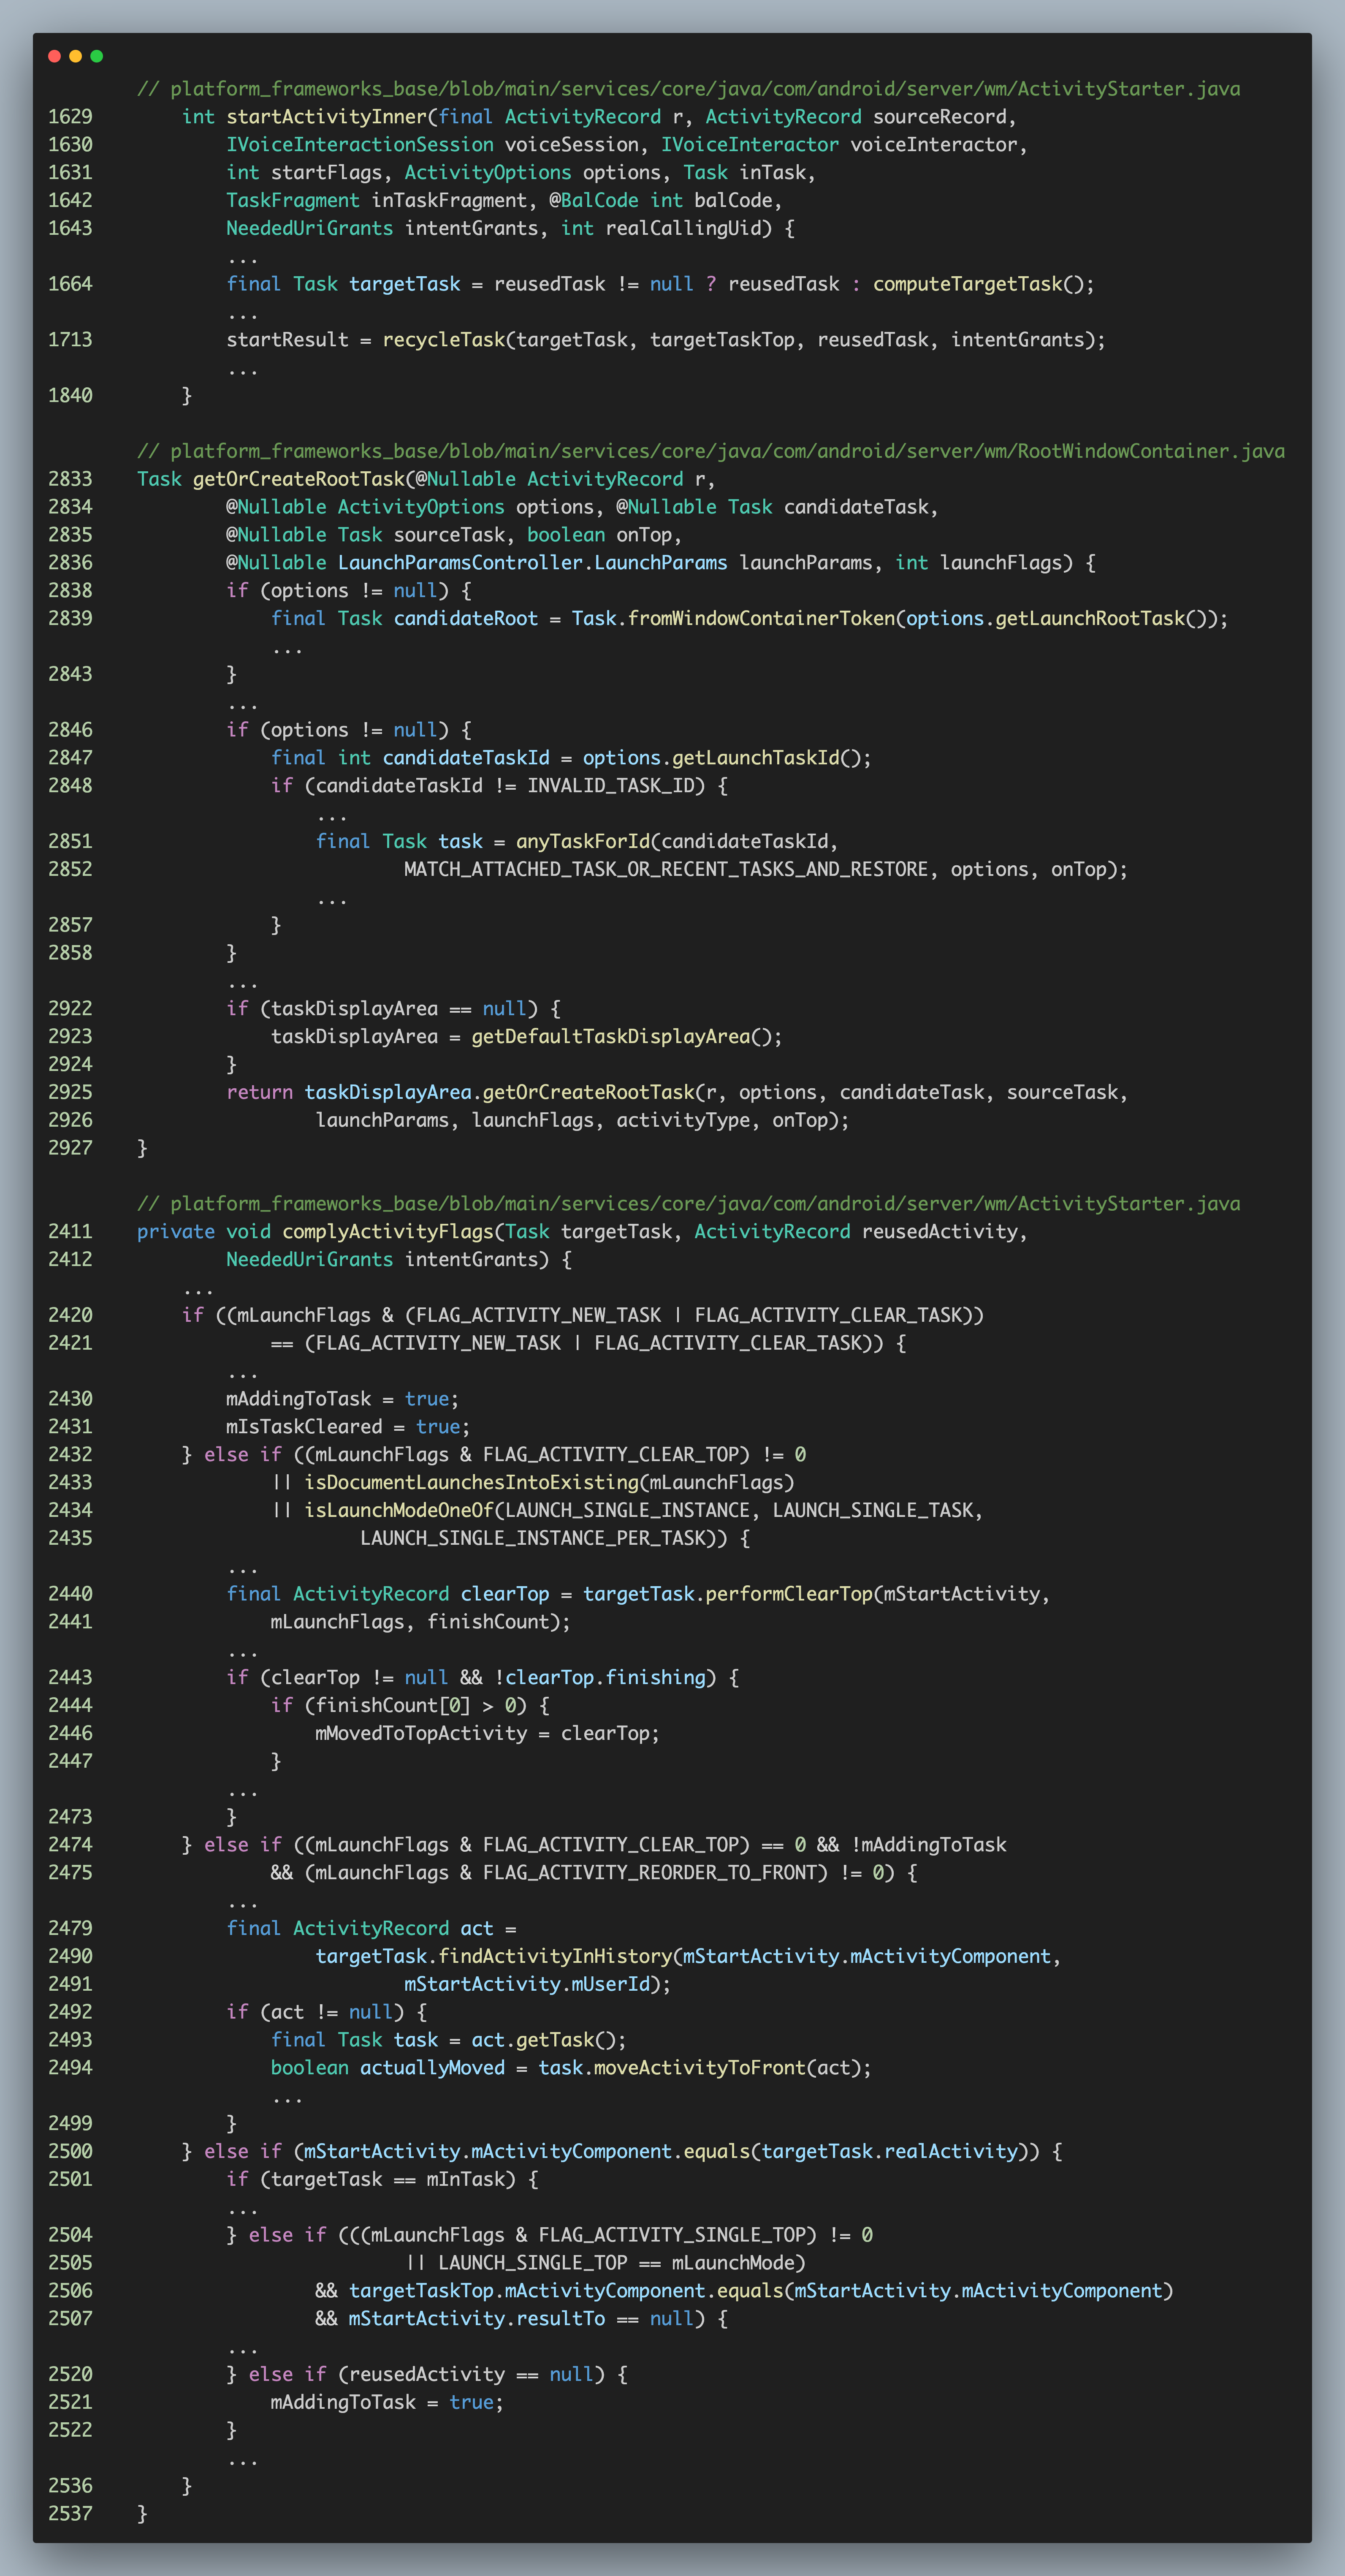
\includegraphics[scale = 0.08]{activity-code.png}
%         \caption{Android system source code for starting activity.}
%     \label{activity-code}
% \end{figure}
% \smallskip

% \begin{figure}[htbp]
%         \centering
%         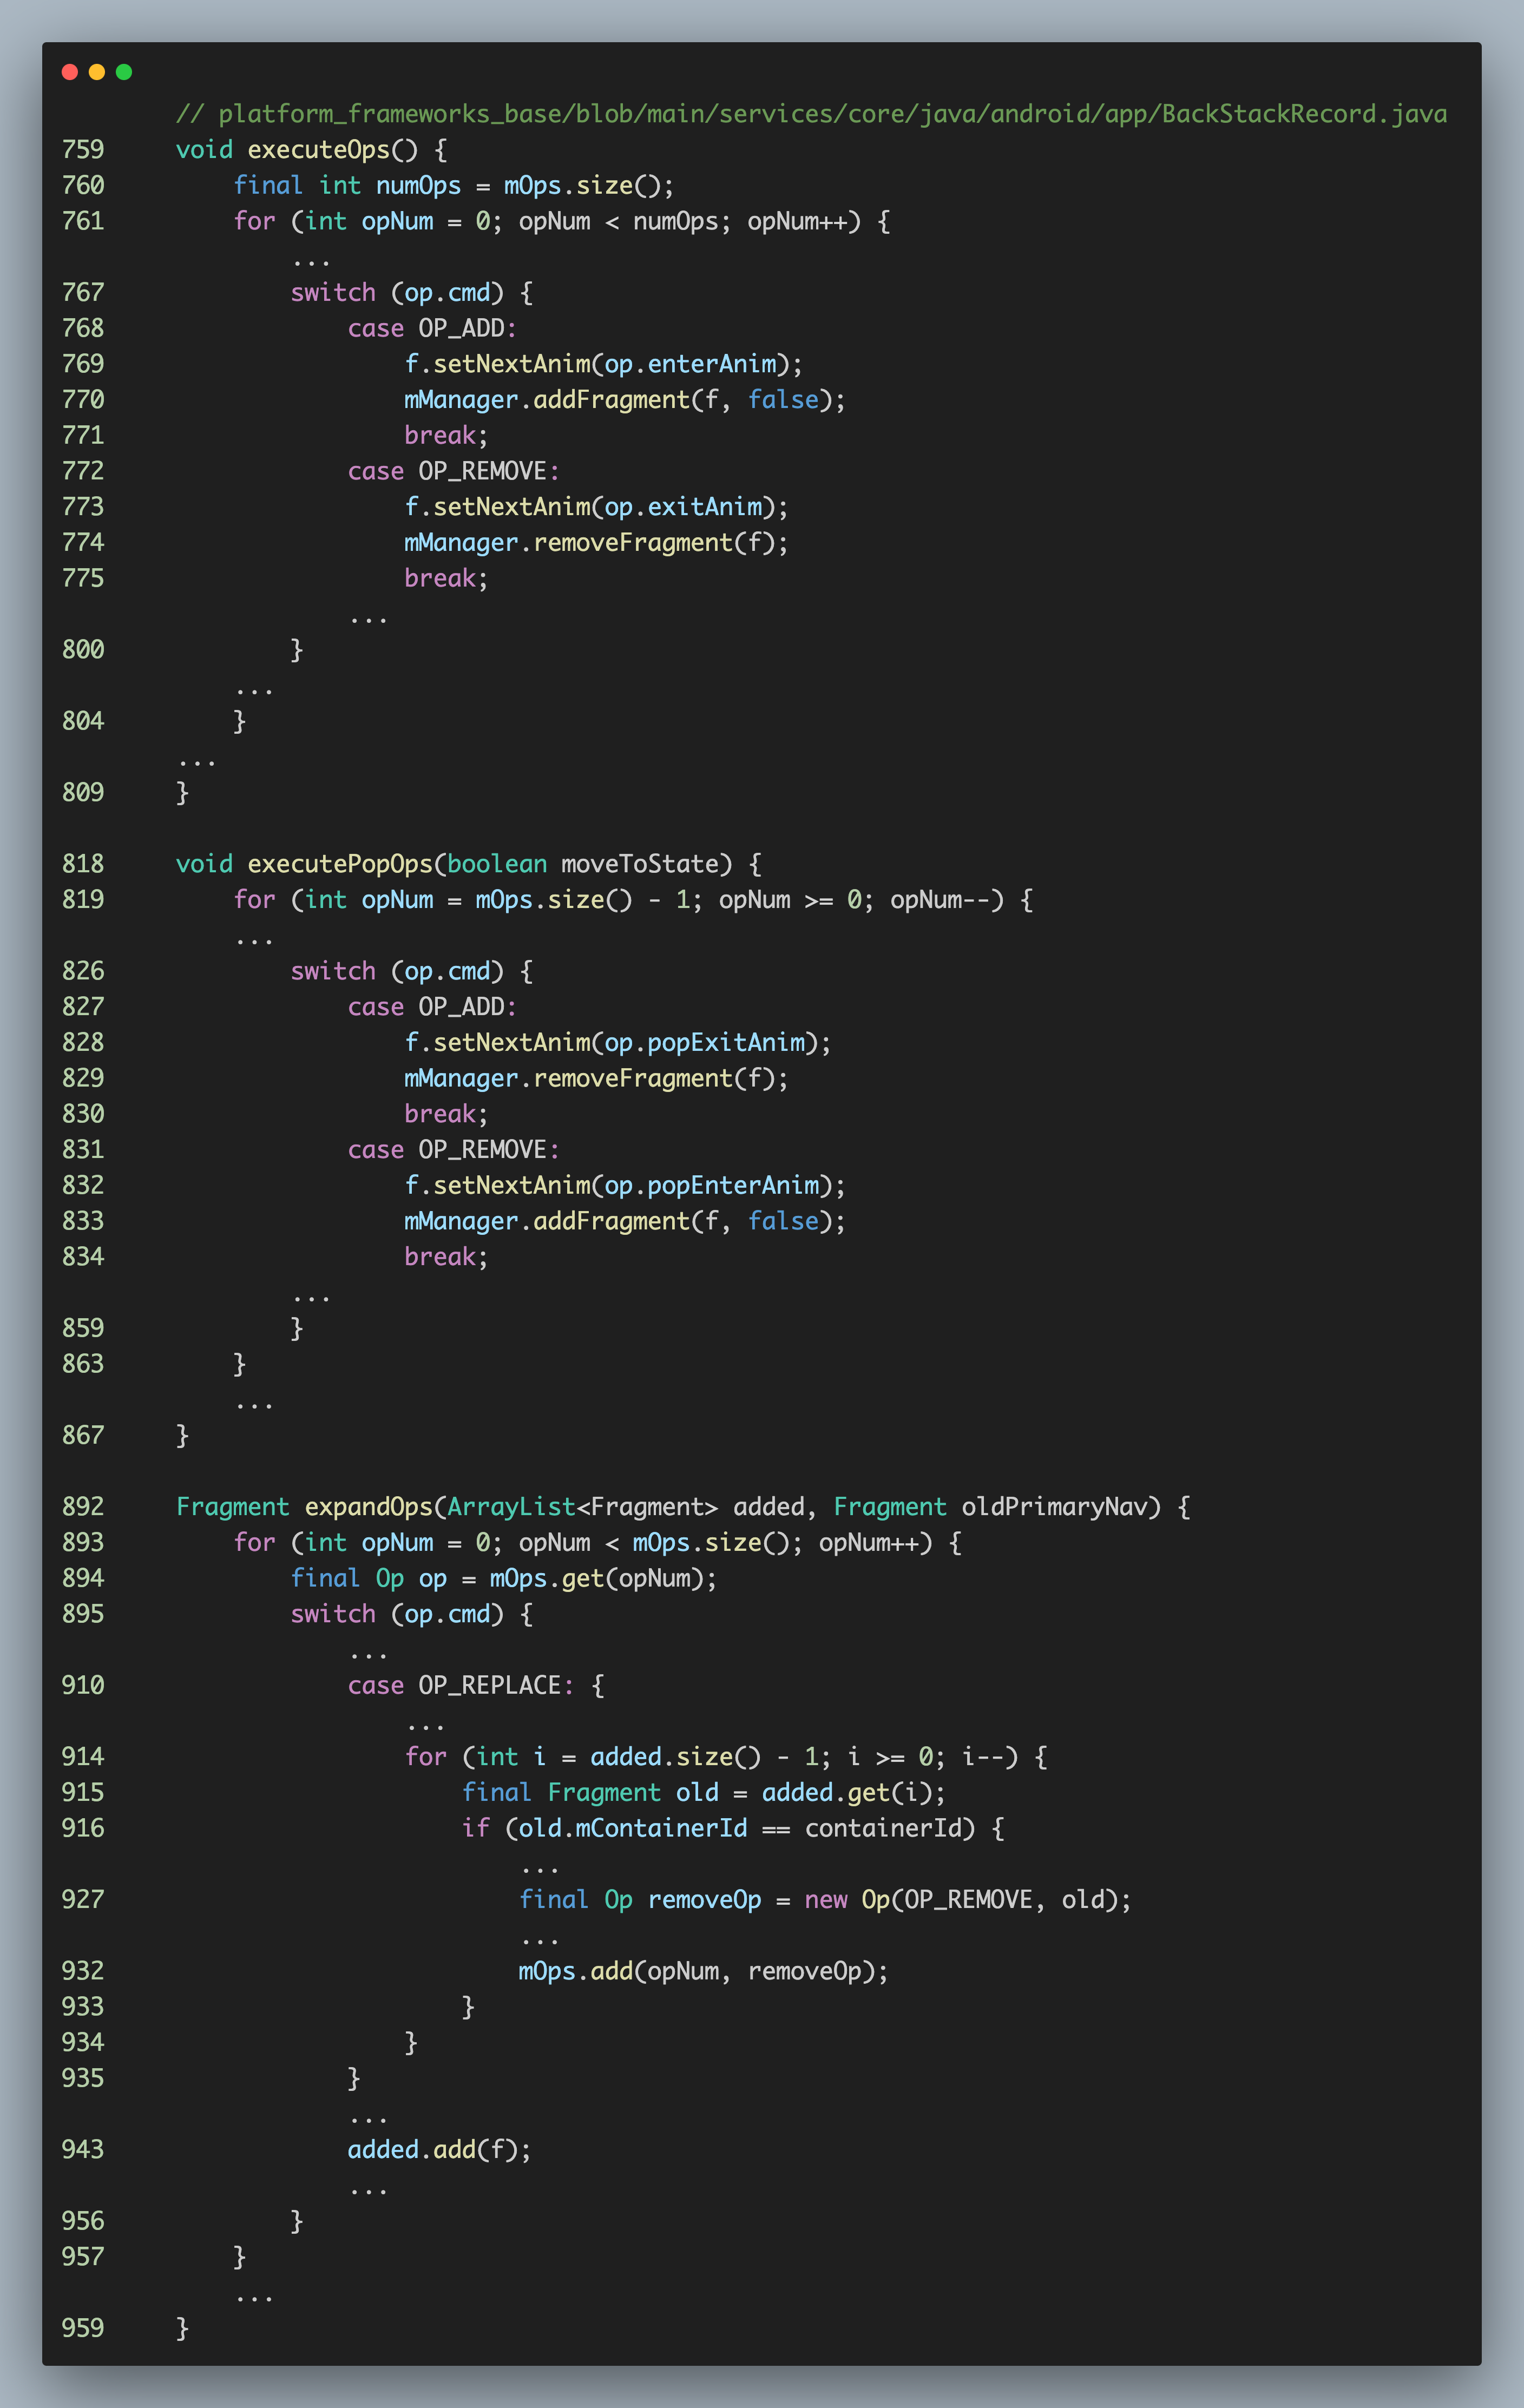
\includegraphics[scale = 0.09]{fragment-code.png}
%         \caption{Android system source code for starting fragment.}
%     \label{fragment-code}
% \end{figure}
% \smallskip


\subsection{Fragment, fragment stack, fragment transaction and fragment transaction stack}

Importantly, activities are \emph{not} an atomic object and may contain sub-components such as %view groups and 
fragments. %which are one of the main focuses here. 
Previous formalism did not address these, but the current paper will (cf.\ Section~\ref{sec:amass}). In a nutshell, %a fragment represents a reusable portion of the app's user interface (UI).  
a fragment represents a modular portion of the user interface within an activity. 
%
%The fragment’s view hierarchy becomes part of, or attaches to, the host’s view hierarchy.
%			
Related to fragments, \emph{view} is a basic building block of UI in Android. Intuitively, a view is a small rectangular box that responds to user inputs (e.g., EditText, Button, CheckBox, etc.) One can simply understand that a fragment serves as a canvas where different views are aggregated which can, for instance, facilitate reuse. Fragments are stored in a fragment container as a stack, which is called \emph{fragment stacks}. Moreover, an activity may maintain several fragment containers. 
 

%A \emph{view group} is an invisible container of views.\footnote{Technically, a view group may contain other view groups, forming a hierarchy. This is however abstracted away in the current paper.} In this paper, a view group is considered to comprise a sequence of fragments.  

%The developer can add fragments % to the activity's view hierarchy 
%either by defining the fragment in the activity's layout file or by defining a (fragment) container in the %your activity's
%layout file and then programmatically adding the fragment from within your activity. 

%In either case, you need to add a FragmentContainerView that defines the location where the fragment should be placed within the activity's view hierarchy. It is strongly recommended to always use a FragmentContainerView as the container for fragments, as FragmentContainerView includes fixes specific to fragments that other view groups such as FrameLayout do not provide.

%\tl{say fragment transaction, to be adpated}

At runtime, an app can add, remove, replace fragments in response to user interaction. 
The add (resp. remove) action will push (resp. pop) a fragment into (resp. out of) a fragment container. The replace action will first remove all the fragments in a fragment container, then push a fragment into it.
%\jinlong{These actions are called fragment actions, for example, an app can add (resp. remove) a fragment in the fragment stack via "add" (resp. "remove") action; it also can clear all fragments in the fragment stack and add a fragment into the fragment stack via "replace" action.}
Multiple fragment actions may be involved in response to one user interaction. Typically, these fragment actions are grouped into \emph{fragment transactions}, where either all the fragment actions are executed,  or none of them is executed. 
%Each set of fragment changes is called a fragment transaction. %, and you can specify what to do inside the transaction using the APIs provided by the FragmentTransaction class. You can 
%Multiple actions can be grouped into a single transaction.
%--for example, a transaction can add or replace multiple fragments. 
%In practice, this is useful when one has multiple sibling fragments displayed on the same screen, such as with split views.
The app can choose to push some fragment transactions into a stack called \emph{fragment transaction stack}, which is used to restore the historical states by cancelling the effects of the fragment transactions in the stack, when a user presses the back button later on.


It is worth emphasizing that, unfortunately, 
the terminologies in literature (such as multitasking, activity stacks, task stacks) are not necessarily consistent. In particular, 
the notion of multitasking is sometimes used to denote the split-screen multitasking where the screen is split into regions to allow several apps displayed simultaneously, moreover, the notion of back stack is widely used in Android documents, but may (misleadingly) refer to any stack regarding the action of pressing the back button. 
In this paper, we use multitasking to denote the fundamental mechanism of the Android operating system that utilizes the task stack, a two-tier stack system, to facilitate smooth switching between tasks, even if the device is not in the spit-screen mode. 
Furthermore, this paper will clarify the notions related to the multitasking mechanism (e.g. tasks and activities) via a proper formalization. 
%We would also like to mention that multitasking discussed in this paper is different from the split-screen multitasking where the screen is split to allow several apps displayed simultaneously. 

It turns out that there are subtle differences between the multitasking mechanisms of different versions of Android. In this paper, we focus on the multitasking mechanisms of the following versions of Android: 6.0, 7.0, 8.0, 9.0, 10.0, 11.0, 12.0 and 13.0. 

% for space
%\iftoggle{fullver}{ 
%	A standard or singleTop activity can be instantiated multiple times leading to duplicated activities in a task. In contrast, an activity with the singleTask or singleInstance launch mode should be instantiated only once. Furthermore, an activity with the singleInstance launch mode is always the root activity of a task. While a singleTask activity
%	can contain other standard or singleTop activities in its task, a singleInstance activity does not contain any other
%	activities in its task. It is the only activity in its task; if it starts another activity, that activity is assigned to a different task. 
%}{}
% for space
%The task affinity attribute specifies to which task the activity prefers to belong. By default, all the activities from the same app have the same affinity (i.e., all activities in the same app prefer to be in the same task). However, one can modify the default affinity of the activity. Android allows a great degree of flexibility: activities defined in different apps can share a task affinity whilst activities defined in the same app can be assigned with different task affinities.  
%
%Android supports inter-component communication via \emph{intents}. An intent is an asynchronous message that activates activities. Android provides 21 intent flags related to activities, but only part of them may govern activity activation. Intent flags are set by caller activities to declare how to activate target activities and are passed to startActivity() or startActivityForResult() as their arguments.

%%%% In this section, we use two examples to motivate this paper. 
%%%% In this section, we use two examples to motivate this paper. 
%%%% In this section, we use two examples to motivate this paper. 
\revision{\section{Motivating examples}\label{sec-motiv-exmp}}
%
We use two simple apps from F-Droid, namely, ``LaunchTime Homescreen''\footnote{available at https://github.com/quaap/LaunchTime/blob/master/} and ``ShoppingList''\footnote{available at https://github.com/GroundApps/ShoppingList/blob/master/}, to motivate this paper. We use the two examples to demonstrate that a model of the Android multitasking mechanism where the various factors related to activities, including launch modes, task affinities, intent flags, the finish() procedure, and the fragments, are taken into account, enables a more accurate static analysis of Android apps.  
%
\subsection{The ``LaunchTime Homescreen'' app}
The ``LaunchTime Homescreen'' app contains ten activities. Let us focus on MainActivity and SettingsActivity. The snippet of the source code of the two activities in the ``LaunchTime Homescreen'' app is shown in Figure~\ref{code-launchtime}. The launch modes of MainActivity and SettingsActivity are singleInstance and standard respectively. 
In line 3942 of the MainActivity.java file (see Figure~\ref{code-launchtime}), MainActivity starts SettingsActivity by calling the function startActivity(settingsIntent), where the settingsIntent contains the intent flag FLAG\_ACTIVITY\_NEW\_TASK. 
On the other hand, in line 142 of the SettingsActivity.java file (see Figure~\ref{code-launchtime}), SettingsActivity starts MainActivity by calling the function startActivity(main), where all the intent flags are set to be false. Moreover, in line 144 of the same file, finish() is called after MainActivity is started. That is, when MainActivity is started, SettingsActivity is finished. 

\begin{figure}[htbp]
    \centering
    \begin{tabular*}{\linewidth}{l}
    \begin{lstlisting}
    // app/src/main/AndroidManifest.xml
    24      <activity
    25          android:name=".MainActivity"
    26          android:configChanges="orientation|keyboardHidden|screenSize"
    27          android:launchMode="singleInstance"
    28          android:windowSoftInputMode="stateHidden|adjustPan">
    29          <intent-filter>
    30              <action android:name="android.intent.action.MAIN" />
                    ...
    35          </intent-filter>
                ...
    47      </activity>
    48      <activity
    49          android:name=".SettingsActivity"
                ...
    55      </activity>

    // app/src/main/java/com/quaap/launchtime/MainActivity.java
    3937    public static void openSettings(Activity activity) {
    3938        Intent settingsIntent = new Intent(activity, SettingsActivity.class);
    3939        settingsIntent.addFlags(Intent.FLAG_ACTIVITY_NEW_TASK);
		...
    3942        activity.startActivity(settingsIntent);
    3943    }

    // app/src/main/java/com/quaap/launchtime/SettingsActivity.java
    139     public boolean onKeyDown(int keyCode, KeyEvent event) {
    140         if(keyCode==KeyEvent.KEYCODE_HOME || keyCode==KeyEvent.KEYCODE_MENU) {
    141             Intent main = new Intent(this, MainActivity.class);
    142             startActivity(main);
    143             setResult(RESULT_OK);
    144             finish();
    145         }
    146         return super.onKeyDown(keyCode, event);
    147     }
    \end{lstlisting}
    \end{tabular*}
    \caption{Source code of the F-Droid app ``LaunchTime Homescreen''}
    \label{code-launchtime}
    \end{figure}

% The ATG of com.quaap.launchtime is shown in Figure~\ref{fig:cmp-atg}, in which the Main and Settings states represent the MainActivity and SettingsActivity respectively. 

Let us consider the task unboundedness problem, that is, whether there is a task where the number of activities in the task can be unbounded, that is, arbitrarily large. In the sequel, we show how the {\AMASS} model provides more precise information than the other models so that we can detect the task unboundedness of  the ``LaunchTime Homescreen'' app more accurately. 
\begin{itemize}
\item If we use the activity transition graph (ATG) to model the ``LaunchTime Homescreen'' app, then the resulting ATG is just a cycle with two vertices MainActivity and SettingsActivity. Then according to the ATG model, we may conclude that the task can become unbounded, since these two activities can start each other indefinitely. 
%
\item If we use the models where the launch modes, task affinities, and intent flags are taken into account, e.g. that in \cite{LHR17}, then the launch modes and intent flags are added as the labels of vertices and edges respectively in the ATG model. That is, the vertices are MainActivity(singleInstance) and SettingsActivity(standard), where the vertex labels (launch models) are put in brackets, and the edge from MainActivity to SettingActivity is labeled by start(NTK) (where start and NTK are the abbreviations of startActivity and FLAG\_ACTIVITY\_NEW\_TASK respectively) and the edge from SettingActivity to MainActivity is labeled by start($\bot$) (where $\bot$ denotes the fact that all the intent flags are false). In this case, compared to the ATG model, more information is available. For instance, we know that there are at most two tasks, one task holding a unique instance of MainActivity (since its launch mode is singleInstance), and the other task holding the instances of SettingsActivity. Nevertheless, we may still conclude that the task where the instances of SettingsActivity belong to can become unbounded, since SettingsActivity can be started by MainActivity for an unbounded number of times. 
%
\item On the other hand, if we use the {\AMASS} model in this paper, then in addition to the launch modes and intent flags, we can also model the finish() procedure. That is, the edge from SettingsActivity to MainActivity is labeled by finishStart($\bot$), where finishStart represents the fact that finish() is called after startActivity() is called. In this case, each time when MainActivity is started by SettingsActivity, SettingsActivity is finished simultaneously. As a result, the task holding SettingsActivity contains at most one instance of SettingsActivity. We conclude that the ``LaunchTime Homescreen'' app does not suffer from the task unboundedness problem actually. 
\end{itemize}
This example motivates us to cover in the {\AMASS} model as much as possible the information about activities, including launch modes, task affinities, and intent flags, as well as the finish() procedure, in order to facilitate a precise static analysis of the Android apps. 
%From this example, we can see that the {\AMASS} model contains more precise information about activities than the well-known ATG model as well as the others models in the literature e.g. that in \cite{LHR17}, thus it enables a more accurate analysis of the task unboundedness problem. 

%%%%%%%%%%%%%%%%%%%%%%%%%%%%%
%%%%%%%%%%%%%%%%%%%%%%%%%%%%%
\hide{
Figure~\ref{fig:cmp-models} shows three models for the app LaunchTime Homescreen, Figure~\ref{fig:cmp-atg} is ATG, the first and simplest model of Android multitasking mechanism, Figure~\ref{fig:cmp-lhr} is the model proposed in \cite{LHR17}, and Figure~\ref{fig:cmp-amass} is AMASS.
In these three models, the Main and Settings states represent the MainActivity and SettingsActivity respectively, and $\SIT$ (resp. $\STD$) in Figure~\ref{fig:cmp-lhr} and Figure~\ref{fig:cmp-amass} represents the launch mode of MainActivity (resp. SettingsActivity). Moreover, the edges in the models represent the relation between activities, $\ntkflag$ represents the intent flags FLAG\_ACTIVITY\_NEW\_TASK, $\finishstart$ represents the combination of startActivity() and finish().
The differences among the three models are that, 1) ATG only consider the relation between activities, ignores the launch modes of activity, the intent flags when starting activity and finish() function, 2) the model of \cite{LHR17} ignores the finish() function.

    \begin{figure}[htbp]
        \subfigure[ATG] {
        \begin{minipage}[t]{0.31\linewidth}
            \centering
            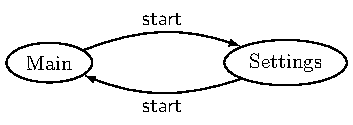
\includegraphics[width=1.9in]{act-running-example1.pdf}
            \label{fig:cmp-atg}
        \end{minipage}
        }
        \subfigure[\cite{LHR17}] {
        \begin{minipage}[t]{0.31\linewidth}
            \centering
            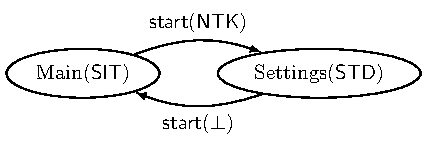
\includegraphics[width=1.9in]{act-running-example2.pdf}
            \label{fig:cmp-lhr}
        \end{minipage}
        }
        \subfigure[AMASS] {
        \begin{minipage}[t]{0.31\linewidth}
            \centering
            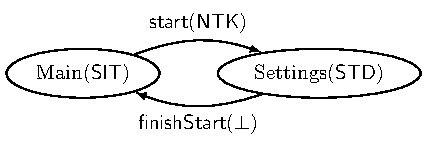
\includegraphics[width=1.9in]{act-running-example3.pdf}
            \label{fig:cmp-amass}
        \end{minipage}
        }
        \caption{Different models for the app LaunchTime Homescreen }
        \label{fig:cmp-models}
    \end{figure}

In the sequel, we consider the task unboundedness problem of these models, that is deciding whether the number of activities in some task will be unbounded. 
\begin{itemize}
	\item In ATG, MainActivity and SettingsActivity will be in a task, MainActivity (resp. SettingsActivity) will be pushed into task by the lower (resp. upper) edge. Therefore there exists a task is unbounded in ATG.
	\item In the model of \cite{LHR17}, MainActivity and SettingsActivity will be placed in two different tasks, since the launch mode of  MainActivity is singleInstance, the number of MainActivity is at most 1. However each time the upper edge is called, SettingsActivity will be pushed into a task, leading to the task unboundedness.
	\item In AMASS, we assume that the label of lower edge is $\startactivity(\bot)$ first, since the real activity of the task containing SettingsActivity is SettingsActivity, SettingsActivity will not be pushed into the task which contains SettingsActivity when the upper edge is called. Therefore, even though finish() function is ignored in AMASS, the task of SettingsActivitys is still bounded. If we do not consider the real activity, only consider the finish() function, the task of SettingsActivitys is still bounded, since when the lower edge is called, SettingsActivity will be finished.
\end{itemize}
Therefore, we can see that ATG and the model of \cite{LHR17} will report the task unboundedness when analyzing the app LaunchTime Homescreen, but either the number of MainActivity or SettingsActivity will be bounded when the app LaunchTime Homescreen is running.
}
%%%%%%%%%%%%%%%%%%%%%%%%%%%%%
%%%%%%%%%%%%%%%%%%%%%%%%%%%%%

%
\subsection{The ``ShoppingList'' app}
If a model of Android multitasking mechanism does not capture the fragments, then the fragment-container unboundedness problem will be missed in the static analysis of Android apps. 
Furthermore, if the fragments are captured, but in an imprecise way, then the static analysis may still be inaccurate. Let us use the ``ShoppingList'' app to illustrate this point. 
The ``ShoppingList'' app comprises two activities, MainActivity and SettingsActivity. The MainActivity contains five Fragments. Let us focus on three of them, namely, ErrorFragment, ShoppingListFragment and CacheListFragment. From the snippet of the source code in Figure~\ref{code-shoplist}, ErrorFragment can start ShoppingListFragment and CacheListFragment via replace() function (see line 69 and 75 of the ErrorFragment.java file). On the other hand, ShoppingListFragment can start ErrorFragment via replace() function (see line 392 of the ShoppingListFragment file). 
%
\begin{itemize}
\item If an imprecise model for fragments, e.g. the AFTG model in \cite{CHGD18}, is used, then we may wrongly reports that ``ShoppingList'' app suffers from the fragment-container unboundedness problem. The AFTG model extends the ATG model by taking the fragments into consideration and consider all the transitions between them. Nevertheless, the AFTG model does not distinguish between the add and replace actions. As a result, from the existence of a cycle between ErrorFragment and ShoppingListFragment in the AFTG model, we may report that the ``ShoppingList'' app is fragment-container unbounded. 
%
\item On the other hand, if the {\AMASS} model is used, then we can add labels to the edges in the AFTG model and distinguish between the add and replace actions. Then we know that the two edges between ErrorFragment and ShoppingListFragment are both labeled by the replace action. As a result, before ErrorFragment or ShoppingListFragment is pushed to the fragment container, the fragment container is emptied. We conclude that the cycle between ErrorFragment or ShoppingListFragment does not lead to the fragment-container unboundedness problem. 
\end{itemize}
This example motivates us to capture the information about fragments, in particular, distinguish between different fragment actions, in the definition of the {\AMASS} model.

%%%%%%% removed %%%%%%%%%
%%%%%%% removed %%%%%%%%%
\hide{
Figure~\ref{fig:cmp-models-frg} shows two models for the app ShoppingList, Figure~\ref{fig:cmp-aftg} is AFTG and Figure~\ref{fig:cmp-amass-frg} is AMASS. 
In these two models, the Error, ShoppingList and CacheList states represent the ErrorFragment, ShoppingListFragment and CacheListFragment respectively, the edges represent the relation between fragments. Moreover the label $\REP$ of the edge in Figure~\ref{fig:cmp-amass-frg} represents the function replace(). 
AFTG only considers the relation between fragments, ignores the function replace(). In the sequel, we consider the fragment stack unboundedness problem of AFTG and AMASS, that is deciding whether the number of fragments in some fragment stack will be unbounded.
\begin{itemize}
	\item In AFTG, ErrorFragment (resp. ShoppingListFragment) will be pushed into the fragment stack by the edge (ShoppingList, Error) (resp. (Error, ShoppingList)). Therefore the fragment stack is unbounded.
	\item In AMASS, when starting ErrorFragment (resp. ShoppingListFragment) by the edge (ShoppingList, $\REP$, Error) (resp. (Error, $\REP$, ShoppingList)), the fragment stack will be cleared first, hence the number of fragments will be only 1.
\end{itemize}
Therefore, we can see that AFTG will report the fragment stack unboundedness when analyzing the app ShoppingList, but AMASS will not.
}
%%%%%%% removed %%%%%%%%%
%%%%%%% removed %%%%%%%%%

\begin{figure}[htbp]
    \centering
    \begin{tabular*}{\linewidth}{l}
    \begin{lstlisting}
    // app/src/main/java/org/janb/shoppinglist/fragments/ErrorFragment.java 
    63      public void onClick(View view) {
    64          android.app.FragmentManager fragmentManager = getFragmentManager();
    65          FragmentTransaction transaction = fragmentManager.beginTransaction();
    66          switch (view.getId()) {
    67              case R.id.error_btn_retry:
    68                  ShoppingListFragment listFR = new ShoppingListFragment();
    69                  transaction.replace(R.id.fragment_container, listFR);
    70                  transaction.addToBackStack(null);
    71                  transaction.commit();
    72                  break;
    73              case R.id.error_btn_cache:
    74                  CacheListFragment cacheFR = new CacheListFragment();
    75                  transaction.replace(R.id.fragment_container, cacheFR, "CACHE_FRAGMENT");
    76                  transaction.addToBackStack(null);
    77                  transaction.commit();
    78                  break;
                    ...
    83          }
    84      }
    // app/src/main/java/org/janb/shoppinglist/fragments/ShoppingListFragment.java 
    378     public void onError(ResponseHelper error) {
                ...
    385         ErrorFragment errFR;
                ...
    390         FragmentManager fragmentManager = getFragmentManager();
    391         FragmentTransaction transaction = fragmentManager.beginTransaction();
    392         transaction.replace(R.id.fragment_container, errFR);
    393         transaction.addToBackStack(null);
    394         transaction.commitAllowingStateLoss();
    395     }

    \end{lstlisting}
    \end{tabular*}
    \caption{Source code of the F-Droid app ``ShoppingList''}
    \label{code-shoplist}
    \end{figure}


%%%%%%%%%%%%%
%%%%%%%%%%%%%
\hide{
    \begin{figure}[htbp]
        \subfigure[AFTG] {
        \begin{minipage}[t]{0.47\linewidth}
            \centering
            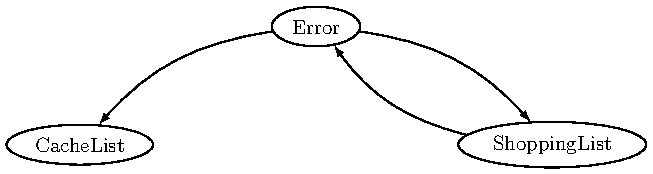
\includegraphics[width=2.5in]{frag-running-example1.pdf}
            \label{fig:cmp-aftg}
        \end{minipage}
        }
        \subfigure[AMASS] {
        \begin{minipage}[t]{0.47\linewidth}
            \centering
            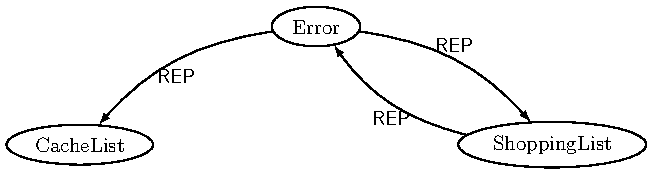
\includegraphics[width=2.5in]{frag-running-example2.pdf}
            \label{fig:cmp-amass-frg}
        \end{minipage}
        }
        \caption{Different models for the app ShoppingList }
        \label{fig:cmp-models-frg}
    \end{figure}
}

\section{Android MultiTasking Stack Systems} \label{sec:amass}
%!TEX root = main.tex

In this section, we introduce \textbf{A}ndroid \textbf{M}ultit\textbf{A}sking \textbf{S}tack \textbf{S}ystem (\AMASS), a formal model to capture the Android multitasking mechanism. Our presentation is inspired by the previous work~\cite{ChenHSWWY18,HCWWY19}, but the model significantly deviates from the ASM therein. Throughout the paper, we let $[m]=\{1, \cdots, m\}$, $\Nn$ be the set of natural numbers, and $\PosNat$ be the set of positive natural numbers. 

Following the overview of Section~\ref{sec:amm}, we shall concentrate on the launch mode, the task affinity, the intent flags when an activity is launched, and the fragment transaction when a fragment is started.  
\begin{itemize}
\item There are four launch modes in Android: ``standard ($\STD$)'', ``singleTop ($\STP$)'', ``singleTask ($\STK$)'' and ``singleInstance ($\SIT$)''.  We shall consider all of them. 
%
\item As mentioned before, we focus on 10 intent flags in this paper, namely, 
\begin{itemize}
\item $\rm FLAG\_ACTIVITY\_NEW\_TASK$ ($\ntkflag$),
\item $\rm FLAG\_ACTIVITY\_NEW\_DOCUMENT$ ($\ndmflag$),
\item $\rm FLAG\_ACTIVITY\_MULTIPLE\_TASK$ ($\mtkflag$),
\item $\rm FLAG\_ACTIVITY\_SINGLE\_TOP$ ($\stpflag$),
\item $\rm FLAG\_ACTIVITY\_REORDER\_TO\_FRONT$ ($\rtfflag$),
\item $\rm FLAG\_ACTIVITY\_CLEAR\_TOP$ ($\ctpflag$),
\item $\rm FLAG\_ACTIVITY\_CLEAR\_TASK$ ($\ctkflag$),
\item $\rm FLAG\_ACTIVITY\_PREVIOUS\_IS\_TOP$ ($\pitflag$),
\item $\rm FLAG\_ACTIVITY\_NO\_HISTORY$ ($\nohflag$),
\item $\rm FLAG\_ACTIVITY\_TASK\_ON\_HOME$ ($\tohflag$).	
\end{itemize}

\item There are three actions in fragment transaction: ``add ($\ADD$)'', ``replace ($\REP$)'' and ``remove ($\REM$)'', and we consider all of them. 
The semantics of these actions are related to the identifiers of fragment instances which we assume are from $\PosNat$. 
\end{itemize}
%In this paper, we consider the ADD and REP actions. The introduction of the REM action would make the  definition of the semantics much more complicated and is left as the future work.  
Moreover, for fragment transactions, we use the tag {\opstack} (resp.\ {\nopstack}) to represent the fact that a fragment transaction will be pushed (resp.\ will not be pushed) to the fragment transaction stack. 

All the abbreviations and their full names are summarized in Table~\ref{tab-abr-full} to facilitate the later references. Note that $\STP$ is used as abbreviations both for the SingleTop launch mode and for the $\rm FLAG\_ACTIVITY\_SINGLE\_TOP$ intent flag. This is acceptable since it is usually clear from the context whether $\STP$ denotes a launch mode or an intent flag.


\begin{table}[htbp]
    \centering
    \begin{tabular}{| c | c |}
    \hline
    \textbf{Abbreviation}  & \textbf{Full name} \\
    \hline
    $\STD$ & Standard  \\
    \hline
    $\STP$ & SingleTop \\
    \hline
    $\STK$ & SingleTask \\
    \hline
    $\SIT$  & SingleInstance \\
    \hline
    $\stpflag$ & $\rm FLAG\_ACTIVITY\_SINGLE\_TOP$\\
    \hline
    $\ctpflag$ &  $\rm FLAG\_ACTIVITY\_CLEAR\_TOP$ \\
    \hline
    $\rtfflag$ & $\rm FLAG\_ACTIVITY\_REORDER\_TO\_FRONT$ \\
    \hline
    $\ntkflag$ & $\rm FLAG\_ACTIVITY\_NEW\_TASK$ \\
    \hline
    $\ndmflag$ & $\rm FLAG\_ACTIVITY\_NEW\_DOCUMENT$\\
    \hline
    $\mtkflag$ & $\rm FLAG\_ACTIVITY\_MULTIPLE\_TASK$  \\
    \hline
    $\ctkflag$ & $\rm FLAG\_ACTIVITY\_CLEAR\_TASK$  \\
    \hline
    $\pitflag$ & $\rm FLAG\_ACTIVITY\_PREVIOUS\_IS\_TOP$ \\
    \hline
    $\nohflag$ & $\rm FLAG\_ACTIVITY\_NO\_HISTORY$ \\
    \hline
%    $\rtnflag$ & $\rm FLAG\_ACTIVITY\_RESET\_TASK\_IF\_NEEDED$ \\
%    \hline
    $\tohflag$ &$\rm FLAG\_ACTIVITY\_TASK\_ON\_HOME$ \\
    \hline
    $\ADD$ & add \\
    \hline
    $\REP$ & replace \\
    \hline
    $\REM$ & remove \\
    \hline
    $\opstack$ & added to the fragment transaction stack \\
    \hline
    $\nopstack$ & not added to the fragment transaction stack \\
    \hline
    \end{tabular}
    \caption{Abbreviations and their full names}
    \label{tab-abr-full}
\end{table}



%\hide{
%\begin{table*}
%	\centering
%\begin{tabular}{c|c}
%Notation & Explanation\\
%\hline
%$\flagset$ & intent flags, $\ntkflag, \ctpflag, \stpflag, \ctkflag, \mtkflag, \rtfflag, \tohflag$\\
% $\frag$   & a set of fragments\\
% $\vgr: \act \rightarrow \Nn^+$ &  {\container} function\\
% $\actinstr$ & $\{\alpha(A, \phi) \mid \alpha \in  \{\startactivity, \finishstart\}, A \in \act, \phi \in \bool(\flagset)\}$\\
% $\fraginstr $ & $\{\mu[O] \mid  \mu \in \{\opstack, \nopstack\}, O \in \ops\}$ \\
% $\ops$ &  a finite set of \emph{macro-transactions} of the form $(\beta_1(F_1, i_1), \cdots, \beta_k(F_k, i_k))$\\
% $V$ &  container\\
% $S= [(A_1, \Theta_1), \cdots, (A_n, \Theta_n)]$ & task
%\end{tabular}
%\caption{A list of notations}
%\end{table*}
%}

Let $\flagset=\{\ntkflag,\ndmflag,\mtkflag, \stpflag,\rtfflag,\ctpflag, \ctkflag,\pitflag,\nohflag,\tohflag\}$ denote the set of intent flags, $\bool(\flagset)$ denote the set of formulae $\phi = \bigwedge \limits_{F \in \flagset} \theta_F$, where $\theta_F = F$ or $\neg F$. For convenience, we use $\bot$ to denote $ \bigwedge \limits_{F \in \flagset} \neg F$. 

\begin{definition}[Android Multitasking Stack System, \AMASS] \label{def:afsm}
An {\AMASS} is a tuple 
$$\Mm = (\act, A_0,\frag, \lmd, \aft, \vgr, \Delta),$$ where 
\begin{itemize}
\item $\act$ is a finite set of activities, and $A_0 \in \act$ is the main activity, let $m=|\act|$,
\item $\frag$ is a finite set of fragments, 
\item $\lmd : \act \rightarrow \{\standard,\singletop,\singletask,\singleinstance\}$ is the launch-mode function,
%
\item $\aft : \act \rightarrow [m]$ is the task-affinity function,
%
\item $\vgr: \act \rightarrow \Nn^*$ is the fragment {\container} function that assigns to each activity a finite sequence of mutually-distinct fragment {\container} identifiers,
% 
%\item $\vgr: \act \rightarrow 2^{\Nn}$ is the view-group function, 
%
\item $\Delta \subseteq (\act \cup \frag) \times ( \actinstr \cup \fraginstr)\cup\{\back\}$ is a finite set of transition rules. Here $\actinstr =$ 
$$\{\alpha(A, \phi) \mid \alpha \in  \{\startactivity, \finishstart\}, A \in \act, \phi \in \bool(\flagset)\}$$ 
and $\fraginstr =  \{\mu[T] \mid  \mu \in \{\opstack, \nopstack\}, T \in \ops\}$ where $\ops$ is a finite set of fragment transactions of the form $(\beta_1(F_1, i_1, x_1), \cdots, \beta_k(F_k, i_k, x_k))$ where for every $j \in [k]$, $\beta_j \in \{\ADD, \REP, \REM\}$, $F_j \in \frag$, $i_j \in \Nn$, and $x_j$ is a variable storing the identifiers of fragment instances.
%$(\beta_1(F_1, i_1), \cdots, \beta_k(F_k, i_k))$ such that for each $j \in [k]$, $\beta_j \in \{\ADD,\REM, \REP\}$, $F_j \in \frag$, and $i_j \in \Nn$. 
\end{itemize}
%
Moreover, we consider several sub-models of {\AMASS}, namely, \emph{activity-oriented} {\AMASS} ($\AOAMASS$) and \emph{fragment-oriented} {\AMASS} ($\FOAMASS$), where all the transition rules are on the activity-level and fragment-level respectively. More precisely, an $\AOAMASS$ (resp. $\FOAMASS$) is an {\AMASS} where all transitions are \emph{activity-oriented}, that is, $\Delta \subseteq \act \times \actinstr \cup \{\back\}$  (resp. \emph{fragment-oriented}, $\Delta \subseteq \frag \times \fraginstr \cup \{\back\}$).
\end{definition}

%
For readability, we write a transition rule $(A, \alpha(B, \phi))\in \Delta$ as $A \xrightarrow{\alpha(\phi)} B$
%$(A, \startactivity(B, \phi))$ as $A \xrightarrow{\startactivity} (B, \phi)$, similarly for $(A, \finishstart(B, \phi))$, and so on. Moreover, we write 
and 
$(A, \mu[T])\in \Delta$ as $A \xrightarrow{\mu} T$. 
%We call $A$ as the \emph{source} of the transition rule. Similarly for the transition rules starting from $F$.
Therefore, all the transitions in an $\AOAMASS$ (resp. $\FOAMASS$), except $\back$, are of the form $A \xrightarrow{\alpha(\phi)} B$ (resp. $A \xrightarrow{\mu} T$).



%%%%%%%%%%%%%%%%%%%%%%%%%%%%%%%%%%%%%%%%%%
%%%%%%%%%%%%%%%%%%%%%%%%%%%%%%%%%%%%%%%%%%
%\hide{
%\begin{example}\label{exmp-running}
%Let $\Mm = (\act, A_0, \frag,\vgr,\lmd,\aft,\Delta)$ be the {\AMASS} illustrated in Figure~\ref{fig-amass},
%where 
%\begin{itemize}
%\item $\act = \{A_0, A_1, B_0,B_1\}$, the main activity is $A_0$, 
%\item $\frag= \{F_0, F_1\}$, 
%\item $\vgr(A_0) = (1)$, $\vgr(A_1) = \vgr(B_0) = \vgr(B_1)  = \epsilon$, 
%\item $\lmd(A_0) = \lmd(A_1) = \lmd(B_0) = \lmd(B_1) = \standard$,
%\item $\aft(A_0) = \aft(A_1)= 0$, $\aft(B_0) = \aft(B_1) = 1$, and
%\item $\Delta$ comprises the rules
%	$\tau_1=A_0 \xrightarrow{\startactivity} (A_1, \bot)$,
%	$\tau_2=A_0 \xrightarrow{\startactivity} (B_0, \ntkflag)$,
%	$\tau_3=A_0 \xrightarrow{\startactivity} (B_1, \ntkflag)$,
%	$\tau_4=B_0 \xrightarrow{\startactivity} (B_1, \bot)$, 
%	$\tau_5=B_1 \xrightarrow{\startactivity} (A_0, \ntkflag)$,
%	$\tau_6=B_1 \xrightarrow{\startactivity} (A_1, \ntkflag \wedge \ctkflag)$,
%	$\tau_7=A_0 \xrightarrow{\opstack} (\ADD(F_0,1))$,
%	$\tau_8=F_0 \xrightarrow{\nopstack} (\ADD(F_1,1))$,
%	$\tau_9=F_1 \xrightarrow{\opstack} (\REP(F_0,1))$.
%%
%%    $A_0 \xrightarrow{\startactivity} (B_0, \ntkflag)$,
%%    $A_0 \xrightarrow{\startactivity} (B_1, \ntkflag)$,
%%    $B_0 \xrightarrow{\startactivity} (B_1, \bot)$,
%%    $B_1 \xrightarrow{\startactivity} (A_0, \ntkflag)$,
%%    $A_0 \xrightarrow{\opstack} (\ADD(F_0,1))$,
%%   and  $F_0 \xrightarrow{\nopstack} (\ADD(F_1,1))$.
%\end{itemize}
%\end{example}
%}
%%%%%%%%%%%%%%%%%%%%%%%%%%%%%%%%%%%%%%%%%%
%%%%%%%%%%%%%%%%%%%%%%%%%%%%%%%%%%%%%%%%%%

%\begin{figure}[ht]
%    \centering
%    \includegraphics[scale=0.7]{amass-example.pdf}
%    \caption{An example of \AMASS}
%    \label{fig-amass}
%\end{figure}

%\begin{remark}
%This choice is (partially) justified by the fact that in the 3000 mostly download GooglePlay apps, only 9 of them (0.3\%) contains the occurrences of this action.
%\end{remark}
%%%%%%%%%%%%%%%%%%%%%%%%%%%%%%%%%%%%%%%%%%%
%%%%%%%%%%%%%%%%%%%%%%%%%%%%%%%%%%%%%%%%%%%



%%%%%%%%%%%%%% Semantics of AMASS for Android 12.0 %%%%%%%%%%%


\smallskip

The rest of this section is devoted to the semantics of {{\AMASS}. We shall first define the semantics of {\AMASS} for Android 13.0, and consider the semantics for other versions later. 
	
%%%%%%%%%%%%%%%%%%%%%%%%%%%%%%%%%%%%%%%%%%%%%%%%%%%%%%%%%%%%%%%%%%%%%%%%%%%%%%%
\subsection{Semantics of {\AMASS} for Android 13.0}\label{sec-amass-13}
%%%%%%%%%%%%%%%%%%%%%%%%%%%%%%%%%%%%%%%%%%%%%%%%%%%%%%%%%%%%%%%%%%%%%%%%%%%%%%

As the model of {\AMASS} involves both activities and fragments, its semantics is rather involved. In order to ease the understanding, we separate the concerns and define the formal semantics of {$\AOAMASS$} and {$\FOAMASS$} respectively. (The long and detailed definition of the formal semantics of {\AMASS} is presented in the appendix.)  


%We shall first define the semantics of {\AMASS} for Android 12.0, and state the semantics for other versions later. 
%\revision{In light of the complexity of semantics of {\AMASS} and that fragments and activities can be defined separately to some extent, we distinguish two subcases, i.e., Activity-based {\AMASS} and Fragment-based {\AMASS}. The complete semantics are defined in Appendix~\ref{app:semantic}.}
%\revision{

%%%%%%%%%%%%%% Semantics of AOAMASS %%%%%%%%%%%
%%%%%%%%%%%%%% Semantics of AOAMASS %%%%%%%%%%%
%%%%%%%%%%%%%% Semantics of AOAMASS %%%%%%%%%%%

%!TEX root = main.tex

\subsubsection{Semantics of $\AOAMASS$}\label{sec:aoamass}

It turns out that the semantics of $\AOAMASS$ is still complicated due to the complex interplay between launch modes and intent flags. Therefore, in the sequel, we separate the concerns further and consider the two sub-models of $\AOAMASS$, namely $\LMAOAMASS$ and $\IFAOAMASS$, which focus on launch modes and intent flags of $\AOAMASS$ respectively. 
More precisely, 
%
\begin{itemize}
\item an $\LMAOAMASS$ is an $\AOAMASS$ where all the transition rules $A \xrightarrow{\alpha(\phi)} B$ (except $\back$) satisfy that $\phi = \bot$, 
\item an $\IFAOAMASS$ is an $\AOAMASS$ where all the transition rules $A \xrightarrow{\alpha(\phi)} B$ (except $\back$) satisfy that $\lmd(A) = \STD$. 
\end{itemize}
%
To ease the understanding, in the main text, we shall only define the formal semantics of the two sub-models $\LMAOAMASS$ and $\IFAOAMASS$, and omit the definition of the formal semantics of $\AOAMASS$,
%delegate the definition of the formal semantics of $\AOAMASS$ to the appendix, 
since the definition of the semantics of $\AOAMASS$ is rather tedious and we think that $\LMAOAMASS$ and $\IFAOAMASS$ are already sufficient to understand the meanings of the launch modes and intent flags. 

To simplify the presentation, in $A \xrightarrow{\alpha(\phi)} B$, we assume that $\alpha$ is $\startactivity$. The definition of the semantics for the case that $\alpha$ is $\finishstart$ can be found in the appendix. 

%%%%%%%%%%%%%% Semantics of LMAOAMASS %%%%%%%%%%%
%%%%%%%%%%%%%% Semantics of LMAOAMASS %%%%%%%%%%%
%%%%%%%%%%%%%% Semantics of LMAOAMASS %%%%%%%%%%%

\smallskip
\noindent {\bf Semantics of $\LMAOAMASS$}.
\smallskip

We start with the semantics of $\LMAOAMASS$ and assume that $\Mm$ is an $\LMAOAMASS$. 
We first introduce some notations. 

%Before defining the semantics of $\LMAOAMASS$ and $\IFAOAMASS$, we introduce some notations. 

%In this case, we consider activities as atomic objects, so we only consider transaction rules of the form $\back$ and $A\xrightarrow{\alpha(\phi)}B$.}
%\subsection*{Intuitions.}
%The intuitions of the transition rules %(except $\back$) 
%are as follows.  
%\begin{itemize}
%	\item $\startactivity(A, \phi)$ denotes the action where the activity $A$ is started with the intent flag $\phi$.
%	
%	\item $\finishstart(A, \phi)$ is the same as $\startactivity(A, \phi)$, except that the current activity is popped after starting $A$.
%\end{itemize}

\paragraph{Tasks and configurations}
A \emph{task} of $\Mm$ is represented by its activity stack and is encoded as a word $S= [A_1, \cdots, A_n] \in \act^+$, with $A_1$ (resp. $A_n$) as the top (resp. bottom) activity of $S$, $n$ is called the \emph{height} of $S$. 
% We define the \emph{affinity of a task} $S$, denoted by $\aft(S)$, to be $\aft(\btmact(S))$. For $S_1 \in \act^*$ and $S_2 \in \act^*$, we use $S_1 \cdot S_2$ to denote the concatenation of $S_1$ and $S_2$, and $\epsilon$ is used to denote the empty word in $\act^*$. 

A \emph{configuration} of $\Mm$ is encoded as a sequence 
$\rho=(\Omega_1,\cdots,\Omega_n)$, and for each $i \in [n]$, $\Omega_i = (S_i,A_i,\zeta_i)$, $S_i\in\act^*$ is a task, $A_i\in\act$ is the real activity of $S_i$, $\zeta_i\in\{\mainflag,\STK,\SIT\}$ represents how the task $S_i$ is launched. 
% a pair $(\rho, \ell)$, where $\rho=(\Omega_1,\cdots,\Omega_n)$, and for each $i \in [n]$, $\Omega_i = (S_i,A_i,\zeta_i)$, $S_i\in\act^*$ is a task, $A_i\in\act$ is the real activity of $S_i$, $\zeta_i\in\{\mainflag,\ntkflag,\ndmflag,\SIT\}$ represents how the task $S_i$ is launched, and $\ell\in\{0,1\}$ represents the top activity is (resp. \emph{not}) launched with the intent flag $\nohflag$ if $\ell = 1$ (resp. $\ell = 0$).
% $S_i$ is (resp. not) the main task, if $b_i=1$ (resp. $b_i=0$).
% We use $\topact(\rho)$ to denote \emph{the top activity} of $\rho$, namely, the top activity of $S_1$. 
For any activity $A$, we refer to an $A$-task as a task whose real activity is $A$. 
%
The tasks $S_1$ and $S_n$ are called the top and the bottom task respectively. (Intuitively, $S_1$ is the foreground  task.) The symbol $\varepsilon$ is used to denote the empty task stack. 
The \emph{affinity of a task} is defined as the affinity of its real activity. A task $(S_i,A_i,\zeta_i)$ in $\rho$ is called an $\SIT$-task if $\zeta_i = \SIT$. 
%It turns out that the semantics of the transition rules of $\Mm$ can guarantee that for any pair of distinct tasks in $\rho$, if none of their real activities has the $\singleinstance$ (SingleInstance) launch mode, then their affinities should be different. 
%Therefore, the number of tasks in $\rho$, that is, $n$, should be no more than $|\aft(\act \setminus \act_{\singleinstance})| + |\act_{\singleinstance}|$, where $\act_{\singleinstance}$ is the set of activities with the $\singleinstance$ launch mode.

A task is called the \emph{main task} of the task stack if it is the first task that was created when launching the app. Note that the current task stack may \emph{not} contain the main task, since it may have been popped out from the task stack. This notion is introduced since the semantics of {\AMASS} is also dependent on whether the task stack contains the main task.

Let $\conf_\Mm$ denote the set of configurations of $\Mm$. The \emph{initial} configuration of $\Mm$ is $(([A_0],A_0,\mainflag))$. 
%
The \emph{height} of a configuration $\rho$ %a configuration $\rho = ((S_1, A_1), \cdots, (S_m, A_m))$ 
is defined as $\max \limits_{i \in [m]}|S_i|$, where $|S_i|$ is the height of $S_i$. By convention, the height of $\varepsilon$ is defined as $0$. 

Before presenting the formal semantics of $\LMAOAMASS$, we present its intuitions. 
%

\paragraph{Intuitions of the launch modes.}  %We explain the intuitions of the four launch modes. 
We call an activity of the launch mode $\STD$ as an $\STD$-activity, similarly for $\STP$, $\STK$ and $\SIT$. 

\begin{itemize}
\item The $\STD$ mode: When a new $\STD$-activity is started, it will be pushed into the top task. 
%
\item The $\STP$ mode: When a new activity of the $\STP$ mode is started, if the activity is already at the top of the top task, it will reuse this activity. Otherwise, a new activity will be pushed into the top task.
%
\item The $\STK$ mode: When a new activity of the $\STK$ mode is started, it will create the activity at the root of a new task or locates the activity on an existing task with the same affinity. If the activity already exists, then all the activities above it are removed from the task. Otherwise, a new activity will be pushed into the task.
%
\item The $\SIT$ mode: 
Similar to $\STK$, but if such an activity already exists, it will reuse this activity, moreover there is only one activity in the task which was created by starting the same activity.
\end{itemize}

\paragraph{Task allocation mechanism.}
The intuitions of the launch modes are actually not that precise. For instance, when a new $\STD$-activity is stated by an $\SIT$-activity, the $\STD$-activity will not necessarily be pushed to the top task. 
%For instance, an $\SIT$-task only contains one activity,  if the launch modes of the caller and callee activity are $\SIT$ and $\STD$ respectively, then the callee activity is pushed into a non-top task.
Task allocation mechanism is to specify to which task will it be allocated when an activity is launched. Via extensive experiments, we  
identify a crucial notion, i.e., real activity of tasks, 
%in Android 7.0 and later versions, 
%use an attribute of tasks called real activity, which 
which plays a pivotal role in such a mechanism. 
%The real activity of a task is 
%is the activity  which was pushed into the task---as the bottom activity---when the task is created. 
%Intuitively, $A_i$ is the activity which was pushed into the taskwhen the task $S_i$ was created.

Generally speaking, for an activity $B$  which is not to land on the top task, %then the task-searching means go in 
the following three steps will apply: (1) If there is any task whose real activity is $B$, then $B$ will be put on the task. %(search downwards from the top task). 
(2) Otherwise, if there is any task whose real activity has the same \emph{task affinity} as $B$, then $B$ will be put on the task. %first such task (search downwards from the top task). 
(3) Otherwise, a new task is created to hold $B$. In the first two cases, if there are multiple instances, the first occurrence starting from the top task will be selected. 

\paragraph{Real activity and main task.}
When the caller activity is an $\SIT$ activity and the callee activity is an $\STD$ or $\STP$ activity $B$, $B$ will \emph{not} always be pushed into the task $S_i$ which is specified according to the \emph{task allocation mechanism}. Generally speaking, the following steps will apply: (1) If the real activity of $S_i$ is \emph{not} $B$, then $B$ will be pushed into $S_i$. (2) Otherwise, if $S_i$ is the main task, that is, $\zeta_i=\mainflag$, then $B$ will be pushed into $S_i$. (If $S_i$ is not the main task, then $B$ will not be pushed.)

\smallskip

Then we introduce some auxiliary functions and predicates to be used in the formal semantics of $\LMAOAMASS$.

\paragraph{Auxiliary functions and predicates.} To specify the transition relation precisely and concisely, we define the following functions and predicates. 
Let $\rho = (\Omega_1,\cdots,\Omega_n)$ be a configuration with $\Omega_i = (S_i,A_i,\zeta_i)$ for each $i\in[n]$, and $S=[B_1,\cdots,B_m]$ be a task. 
% Let $(\rho,\ell)$ be a configuration with $\rho = (\Omega_1,\cdots,\Omega_n)$ with $\Omega_i = (S_1,A_i,\zeta_i)$ for each $i\in[n]$, and $S=[B_1,\cdots,B_m]$ be a task. 
\begin{itemize}
	%	\item $\realact(S) = A$, where $S$ is created by an action $start(A,\Ff)$
    \item $\topact(S) = B_1$, $\btmact(S) = B_m$, %~\mbox{where}~ S = A(\act^*)$
	%	\item.  %, ~\mbox{where}~ S = (\act^*)A$\push
	\item $\toptsk(\rho) = S_1$,  %this is the foreground task
        $\topact(\rho) = \topact(\toptsk(\rho))$, %, where $S_1 = [A]\cdot S_1'$.
	
    \item $\push(\rho, B) = (([B] \cdot S_1,A_1,\zeta_1), \Omega_2, \cdots, \Omega_n)$,
    	
%	\item $\mvacttop(\rho, B)  =(([B]\cdot S'_1 \cdot S''_1,A_1,\zeta_1), \Omega_2, \cdots, \Omega_n) $, 
%        if $S_1=S'_1 \cdot[B]\cdot S''_1$ with $S'_1 \in (\act \setminus \{B\})^*$,
	%---------------------------------------------------------------------------------------------------------------
    \item $\clrtop(\rho, B) = (([B]\cdot S_1'',A_1,\zeta_1),\Omega_2,\cdots, \Omega_n)$ if $S_1=S'_1 \cdot S''_1$ with $S'_1 \in (\act \setminus \{B\})^*B$,
	
    \item $\clrtsk(\rho, B)  = (([B],A_1,\zeta_1),\Omega_2,\cdots, \Omega_n)$,
	
    \item $\mvtsktop(\rho, i) = (\Omega_i,\Omega_1,\cdots,\Omega_{i-1},\Omega_{i+1},\cdots,\Omega_n)$,

    \item $\newtsk(\rho, B, \zeta)  = (([B],B,\zeta),\Omega_1,\cdots, \Omega_n)$,
	%---------------------------------------------------------------------------------------------------------------
	
	\item $\getrealtsk(\rho, B) = S_i$ such that $i \in [n]$ is the \emph{minimum} index satisfying $A_i = B$ if such an index $i$ exists; $\getrealtsk(\rho, B) = *$ otherwise,
	%---------------------------------------------------------------------------------------------------------------
	
    \item $\gettsk(\rho, B) = S_i$ such that $i \in [n]$ is the \emph{minimum} index satisfying $\aft(A_i)=\aft(B)$ and $\zeta_i \in \{\mainflag,\STK\}$, if such an index $i$ exists; $\gettsk(\rho, B) = *$ otherwise.
	
	%
	%-------------------------------------------------------------------------------------------------
\end{itemize}

The formal semantics of $\Mm$ will be defined as a transition relation $\xrightarrow{\Mm}$. 
%Before the formal definition, 
We first use the following example to illustrate the semantics. 
\begin{example}\label{exam:iff-amass}
    Let $\Mm = (\act, A,\frag,\lmd,\aft,\vgr, \Delta)$ be an $\LMAOAMASS$, where $\act = \{A, B, C, D\}$, the functions $\lmd$ and $\aft$ are defined in Table~\ref{tab-attribute}. 

\begin{table}[htbp]
\begin{center}
    \begin{tabular}{|c|c|c|c|c|c|}
    \hline
    Activity & $\lmd$ & $\aft$\\
    \hline
    $A$ & $\singletask$ & 1 \\
    \hline
    $B$ & $\singletop$ & 2 \\
    \hline
    $C$ & $\singleinstance$ & 1 \\
    \hline
    $D$ & $\standard$ & 2 \\
    \hline
    \end{tabular}
\end{center}
    \caption{Attributes of activities}
    \label{tab-attribute}
    \end{table}
        
Moreover, $\Delta = \{\back, \tau_1, \tau_2, \tau_3, \tau_4, \tau_5\}$, where 
        $\tau_1 = A \xrightarrow{\startactivity(\bot)} B$,
        $\tau_2 = B \xrightarrow{\startactivity(\bot)} C$,
        $\tau_3 = C \xrightarrow{\startactivity(\bot)} D$,
        $\tau_4 = D \xrightarrow{\startactivity(\bot)} A$,
        $\tau_5 = B \xrightarrow{\startactivity(\bot)} B$.
Then the configurations reachable from the initial configuration $(([A], A , \mainflag))$ by executing the transition rules from $\Delta$ are illustrated in Figure~\ref{iff-example}, where the vertices denote the configurations and the edges denote the elements of $\xrightarrow{\Mm}$. 
For instance, 
\begin{itemize}
\item if the transition rule $A \xrightarrow{\startactivity(\bot)} B$ is applied to the configuration $(([A], A , \mainflag))$, then $B$ is pushed,  since $\lmd(B) = \STP$ and $A \neq B$, resulting in the configuration $(([BA], A , \mainflag))$,
%
\item if $B \xrightarrow{\startactivity(\bot)} B$ is applied to the configuration $(([BA], A, \mainflag))$, then $B$ will not be pushed, since $\lmd(B) = \STP$ and the top activity of the top task is $B$, 
%
\item if $B \xrightarrow{\startactivity(\bot)} C$ is applied to the configuration $(([BA], A, \mainflag))$, then a new task $([C], C, \SIT)$ is created, since $\lmd(C) = \SIT$, resulting in the configuration $(([C], C, \SIT), ([BA], A , \mainflag))$,  
%
\item if $C \xrightarrow{\startactivity(\bot)} D$ is applied to the configuration $(([C], C, \SIT), ([BA], A , \mainflag))$, then a new task $([D], D, \STK)$ is created, since $\lmd(C) = \singleinstance$, $\lmd(D) = \STD$ and $\aft(D)  = 2 \neq \aft(A)$, resulting in the configuration
$(([D], D, \STK), ([C], C, \SIT)$, $([BA], A , \mainflag))$, 
%
\item if $D \xrightarrow{\startactivity(\bot)} A$ is applied to the configuration $(([D], D, \STK), ([C], C, \SIT), ([BA], A , \mainflag))$, then the task $([BA], A , \mainflag)$ is moved to the top and all the activities above $A$, which is $B$ here, are removed from the task, since $\lmd(A) = \STK$, 
$$\getrealtsk((([D], D, \STK), ([C], C, \SIT), ([BA], A , \mainflag)), A) = ([BA], A , \mainflag),$$ 
and $A$ occurs in $([BA], A , \mainflag)$, resulting in the configuration 
$(([A], A , \mainflag), ([D], D, \STK), ([C], C, \SIT))$, 
%
\item \dots
%
\item if $C \xrightarrow{\startactivity(\bot)} D$ is applied to the configuration $(([C], C, \SIT), ([BA], A , \mainflag), ([D], D, \STK))$, then the task $([D], D, \STK)$ is moved to the top, but $D$ will not be pushed, since $\lmd(C) = \SIT$, $\lmd(D) = \STD$, 
$$\getrealtsk((([C], C, \SIT), ([BA], A , \mainflag), ([D], D, \STK)), D) = ([D], D, \STK),$$
and $([D], D, \STK)$ is not the main task, resulting in  the configuration $(([D], D, \STK), ([C], C, \SIT), ([BA], A , \mainflag))$.
\end{itemize}
Note that for $\Mm$, there are only finitely many configurations reachable from the initial configuration, which may not be the case for $\LMAOAMASS$ in general.  
    % $(([D_1],D_1,1))$\\
    % $\xrightarrow[\tau_1]{\Mm}(([P_1D_1],D_1,1))$\\
    % $\xrightarrow[\tau_2]{\Mm}(([P_1D_1],D_1,1))$\\
    % $\xrightarrow[\tau_3]{\Mm}(([K_2],K_2,0),([P_1D_1],D_1,1))$\\
    % $\xrightarrow[\tau_4]{\Mm}(([D_1K_2],K_2,0),([P_1D_1],D_1,1))$\\
    % $\xrightarrow[\tau_5]{\Mm}(([T_2],T_2,0),([D_1K_2],K_2,0),([P_1D_1],D_1,1))$\\
    % $\xrightarrow[\tau_6]{\Mm}(([K_2],K_2,0),([T_2],T_2,0),([P_1D_1],D_1,1))$\\
    

    
\begin{figure}
    % \vspace{-3mm}
        \centering
        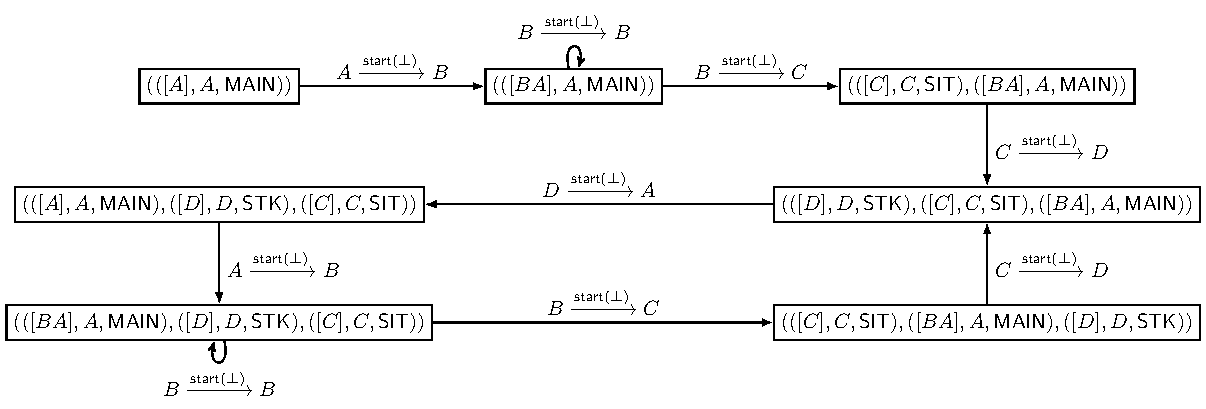
\includegraphics[scale = 0.75]{iff-example.pdf}
        \caption{Configurations reachable from the initial configuration $(([A], A,\mainflag))$ in a $\LMAOAMASS$ $\Mm$}
            %in $\phi$
    % \vspace{-6mm}	
    \label{iff-example}
\end{figure}

    % and $\lmd(D_1) = \lmd(D_2) = \STD$, $\lmd(P_1) = \lmd(P_2) = \STP$, $\lmd(K_1) = \lmd(K_2) = \STK$, $\lmd(T_1) = \lmd(T_2) = \SIT$, and $\aft(D_1) = \aft(P_1) = \aft(K_1) = \aft(T_1) = 1$, $\aft(D_2) = \aft(P_2) = \aft(K_2) = \aft(T_2) = 2$.
\end{example}

From the informal description and the example above, we have already gotten an intuitive understanding of the semantics of $\Mm$. 
To facilitate a precise understanding of the semantics of $\LMAOAMASS$, let us formally define the semantics of $\Mm$ as a transition relation $\xrightarrow{\Mm} $ in the sequel. 

\paragraph{Transition relation.} We define the relation $\xrightarrow{\Mm} $ which comprises the quadruples $(\rho, \tau, \rho') \in \conf_\Mm \times \Delta  \times \conf_\Mm$ 
%$(\rho, \ell) \xrightarrow{\Mm} (\rho', \ell')$ on $\conf_\Mm$ 
to formalise the semantics of $\Mm$. For readability, 
we write $(\rho, \tau, \rho')\in \xrightarrow{\Mm}$  as $\rho \xrightarrow[\tau]{\Mm} \rho'$.
% we write $((\rho,\ell), \tau, (\rho',\ell'))\in \xrightarrow{\Mm}$  as $(\rho,\ell) \xrightarrow[\tau]{\Mm} (\rho',\ell')$.
%Intuitively, $i = 0, 1, 2$ corresponds to the cases that the top task of $\rho$ is absent in $\rho'$, remains to be the top task of $\rho'$, or becomes the task immediately below the top task, of $\rho'$ respectively. 

Let $\rho = ((S_1, A_1, \zeta_1), \cdots, (S_n, A_n, \zeta_n))$ be the current configuration for some $n \ge 1$ and $\topact(\rho) = A$. Moreover, let $S_1 = [A'_1, \cdots, A'_m]$. Evidently, $A = A'_1$.

If $\tau = \back$, then $\rho' = ((S'_1, A_1, \zeta_1), (S_2, A_2, \zeta_2) \cdots, (S_n, A_n, \zeta_n))$ if $m > 1$, where $S'_1 = [A'_2, \cdots, A'_m]$, and $\rho' = ((S_2, A_2, \zeta_2) \cdots, (S_n, A_n, \zeta_n))$ otherwise. 

Then let us consider $\tau = A\xrightarrow{\startactivity(\phi)}B$. 
%\jinlong{put the semantics of $\finishstart$ in Appendix~\ref{app-finishstart-lmaoamss}.}

%Let $\rho = ((S_1, A_1, \zeta_1), \cdots, (S_n, A_n, \zeta_n))$ be the current configuration for some $n \ge 1$ and $\topact(\rho) = A$.

%As the semantics of {\AMASS} are highly complex even if we consider only the semantics of activities separately, hence we will formalize the semantics step by step. Firstly, we consider the case without the intent flag, then we consider the case with only the intent flag, and finally we consider the complete semantics.
%\subsection*{\revision{Case: intent-flag free}}
%In this case, we only consider the launch modes and task affinities, that is, $\phi = \bot$. Launch modes and task affinities are the attributes of an activity, recall that a task is a collection of activities to carry out a certain job, the launch modes are used to define how an activity is associated with the task as Table~\ref{tab-int-lm} shown, and the task affinities are used to define how an activity tends to belong to a particular task. By default, all activities within the same application have the same affinity. Therefore, by default, all activities within the same application tend to be in the same task.

% We consider the subcase $\alpha = \startactivity$ first, the subcase $\alpha = \finishstart$ could be defined according to the former subcase.


\smallskip
\noindent \fbox{$\lmd(B) = \STD$}
	\begin{itemize}
		\item If $\lmd(A) \neq \SIT$, then $\rho'= \push(\rho,B)$.
		%
		\item If $\lmd(A) = \SIT$, then
    		\begin{itemize}
                \item if $\getrealtsk(\rho,B) = S_i$ and $\zeta_i\neq\mainflag$, then $\rho'=\mvtsktop(\rho, i)$,
                \item if $\getrealtsk(\rho,B) = S_i$ and $\zeta_i = \mainflag$, or $\getrealtsk(\rho,B) = *\wedge \gettsk(\rho,B) = S_i$, \\then $\rho'=\push(\mvtsktop(\rho, i),B)$,
    			\item if $\gettsk(\rho, B)=*$, then $\rho'= \newtsk(\rho, B, \STK)$.
    		\end{itemize}
	\end{itemize}

\noindent  \fbox{$\lmd(B) = \STP$}
	\begin{itemize}
		\item  If $\lmd(A) \neq \SIT$, then
        \begin{itemize}
            \item if $A = B$, then $\rho' = \rho$,
            \item otherwise, $\rho' = \push(\rho, B)$.
        \end{itemize}
		%
		\item If $\lmd(A) = \SIT$, then
    		\begin{itemize}
                \item if $\getrealtsk(\rho,B) = S_i$ and $\zeta_i\neq\mainflag$, then $\rho'=\mvtsktop(\rho, i)$,
                \item if $\getrealtsk(\rho,B) = S_i$ and $\zeta_i = \mainflag$, or $\getrealtsk(\rho,B) = *\wedge \gettsk(\rho,B) = S_i$, 
                \begin{itemize}
                    \item if $\topact(S_i) = B$, then $\rho' = \mvacttop(\rho,i)$,
                    \item otherwise $\rho'=\push(\mvtsktop(\rho, i),B)$,
                \end{itemize}
                % then $\rho'=\push(\mvtsktop(\rho, i),B)$,
    			\item if $\gettsk(\rho, B)=*$, then $\rho'= \newtsk(\rho,B, \STK)$.
    		\end{itemize}
	 \end{itemize}
	
\noindent \fbox{$\lmd(B) = \SIT$}
\begin{itemize}
	\item If $\getrealtsk(\rho, B) = S_i$, then $\rho' = \mvtsktop(\rho, i)$.
	\item If $\getrealtsk(\rho, B) = *$, then $\rho' = \newtsk(\rho, B,\SIT)$.
\end{itemize}

\noindent  \fbox{$\lmd(B) = \singletask$}
\begin{itemize}
	\item If $\getrealtsk(\rho, B) = S_i$, or $\getrealtsk(\rho,B) = *\wedge\gettsk(\rho,B) = S_i$ then
	\begin{itemize}
        \item if $B \not \in S_i$, then $\rho' = \push(\mvtsktop(\rho, i), B)$,
        \item if $B \in S_i$, 	then $\rho' =  \clrtop(\mvtsktop(\rho, i), B)$.
	\end{itemize}
\item If $\gettsk(\rho, B) = *$, then $\rho' = \newtsk(\rho, B,\STK)$.
\end{itemize}
From the definition of the semantics, we can see that a new task $([B], B, \STK)$ is created, not only when $\lmd(B) = \STK$, but also when $\lmd(A) = \SIT$ and $\lmd(B) = \STD$.
% \noindent\emph{Case: $\alpha = \finishstart$}

% In this subcase, $A\xrightarrow{\finishstart(\bot)}B$ specifies that $B$ is started followed by the termination of $A$, popped from the task stack. Let $\tau' = A\xrightarrow{\startactivity(\bot)}B$ and $\rho\xrightarrow[\tau']{\Mm}\rho''$ with $\rho''=((S_1',A_1',b_1'),\cdots,(S_{n'}',A_{n'}',b_{n'}'))$.
% \begin{itemize}
%     \item If $A_1\neq A_1'$, it means that the $A_1'$-task is the top task instead of $A_1$-task, hence $A$ is the top activity of $S_2'$, then $\rho' = \rmact(\rho'',2,1)$.
%     \item If $A_1=A_1$, it means that $A_1$-task is still the top task.
%     \begin{itemize}
%         \item if $|S_1|>|S_1'|$, it means that $A$ has popped, then $\rho' = \rho''$,
%         \item if $|S_1|<|S_1'|$, it means that $A$ is the second to top activity of $S_1'$, then $\rho' = \rmact(\rho'',1,2)$,
%         \item if $|S_1|=|S_1'|$, it means that $A$ is the top activity of $S_1'$, then $\rho' = \rmact(\rho'',1,1)$.
%     \end{itemize}
% \end{itemize}

%Finally, let us consider $\tau = A\xrightarrow{\finishstart(\phi)}B$.  
%The semantics of $A\xrightarrow{\finishstart(\phi)}B$ is defined the same as follows: Assume that $\rho \xrightarrow[\tau']{\Mm} \rho''$ where $\tau' = A\xrightarrow{\startactivity(\phi)}B$. Compute the index $(i,j)$ of $A$ in $\rho''$, that is the $j$-th activity of the $i$-th task in $\rho''$ is $A$, then $\rho' = \rmact(\rho'',i,j)$




%%%%%%%%%%%%%% Semantics of IFAOAMASS %%%%%%%%%%%
%%%%%%%%%%%%%% Semantics of IFAOAMASS %%%%%%%%%%%
%%%%%%%%%%%%%% Semantics of IFAOAMASS %%%%%%%%%%%

\smallskip
\noindent {\bf Semantics of $\IFAOAMASS$}.

\smallskip

The intuitions of the intent flags are given in Table~\ref{tab-int-flag}. We would like to warn that although the intuitions of these intent flags may help the readers to get some preliminary idea of their meanings, before diving directly into the formal semantics, they are nonetheless inaccurate, especially when different flags may interfere with each other. 
%, before defining the formal semantics of $\IFAOAMASS$.

\begin{table}[htbp]
\begin{center}
\small
    \begin{tabular}{|m{5.5cm}<{\centering}|m{2cm}<{\centering}|m{6cm}<{\centering}|}
    \hline
    \textbf{Intent Flags} & \textbf{Abbreviation} & \textbf{Intuition} \\
    \hline
	$\rm  FLAG\_ACTIVITY\_SINGLE\_TOP$ & $\stpflag$ & If it is set,  it has the same effect as starting an activity of the $\STP$ launch mode.\\
    \hline
	$\rm FLAG\_ACTIVITY\_CLEAR\_TOP$ & $\ctpflag$ & If it is set,  all the activities above the topmost occurrence of the started activity in the top task will be removed.\\
    \hline
	$\rm FLAG\_ACTIVITY\_REORDER\_TO\_FRONT$ & $\rtfflag$ & If it is set, it will check for the existence of the started activity in the task. If an instance of the activity exists, then the topmost occurrence of this activity will be moved to the top of this task. Otherwise, a new instance of the activity will be pushed into the top task.\\
    \hline
	$\rm FLAG\_ACTIVITY\_NEW\_TASK$ & $\ntkflag$ & If it is set, it will look for an existing task to put the started activity according to the task allocation mechanism. If such a task exists, the task will be moved to the top and a new instance of the activity is pushed to the task, otherwise a new task is created to put this activity.\\
    \hline
	$\rm FLAG\_ACTIVITY\_NEW\_DOCUMENT$ & $\ndmflag$ & If it is set, its behavior is similar to the $\STK$ launch mode, but the task allocation mechanism is slightly different, namely, it will look for an existing task by only using real activities of tasks, but not affinities.\\
    \hline
	$\rm FLAG\_ACTIVITY\_MULTIPLE\_TASK$ & $\mtkflag$ & It is usually used together with $\ntkflag$ or $\ndmflag$. If it is set, then it will always create a new task to put the started activity, no matter whether there already exists a task of the same affinity as this activity.\\
    \hline
	$\rm  FLAG\_ACTIVITY\_CLEAR\_TASK$ & $\ctkflag$ &  It is usually used together with $\ntkflag$ or $\ndmflag$. If it is set, it will remove all the activities in the task and push the started activity to the task.\\
    \hline
	$\rm  FLAG\_ACTIVITY\_NO\_HISTORY$ & $\nohflag$ & If it is set,  when the started activity becomes a non-topmost activity in the future, the activity will be removed.\\
    \hline
	$\rm  FLAG\_ACTIVITY\_PREVIOUS\_IS\_TOP$ & $\pitflag$ & If it is set, then when starting this activity, the activity immediately below the topmost activity will play the role of the topmost activity.\\
    \hline
%	$\rm  FLAG\_ACTIVITY\_RESET\_TASK\_IF\_NEEDED$ & $\rtnflag$ & It is usually used together with $\ntkflag$ or $\ndmflag$. If it is set, the task which has the same affinity with the caller activity will be moved to the top, when the intent flag $\ntkflag$ or $\ndmflag$ is set.\\
%	If set, and this activity is either being started in a new task or bringing to the top an existing task, then it will be launched as the front door of the task.
%    \hline
	$\rm FLAG\_ACTIVITY\_TASK\_ON\_HOME$ & $\tohflag$ & It is usually used together with $\ntkflag$ or $\ndmflag$. If it is set, then only the top task, which is either a newly created task or an existing task moved to the top, is kept, and all the other tasks are removed. \\
    \hline
    \end{tabular}
\end{center}
    \caption{Intuitions of intent flags}
    \label{tab-int-flag}
\end{table}

%\jinlong{omit $\nohflag$ here, and give an intuition of the $\nohflag$, the details defined in Appendix~\ref{app-ifaoamass}.}

To ease the presentation, let us assume that $\phi\models \neg \nohflag$ in $A \xrightarrow{\startactivity(\phi)} B$. The full semantics of $\IFAOAMASS$ where the situation $\phi \models \nohflag$ is taken into consideration can be found in Appendix~~\ref{app-ifaoamass}.


%To define the semantics of $\IFAOAMASS$, we adapt slightly the notion of configurations and add some auxiliary functions and predicates. 
Let $\Mm$ be an $\IFAOAMASS$, namely, $\lmd(A) = \STD$ for each activity $A$.



%It turns out that the flag $\nohflag$ makes the definition of the semantics tedious. For instance, if the current top activity of the top task is started with the flag $\nohflag$, then it should be removed if it is not the top activity of the top task anymore after the application of a transition rule. To ease the understanding, we omit the flag $\nohflag$ first, and give a intuition of the semantics of $\Mm$ with $\nohflag$ later, the details of the formal semantics of $\Mm$ is defined in Appendix~\ref{app-ifaoamass}.
%Moreover we can largely reuse the definition of semantics of the case $\phi\models\neg\tohflag$. 
%In the sequel, $\nohflag$ is ignored first, and we distinguish two subcases, i.e., $\phi \models \neg \tohflag$ and $\phi \models \tohflag$.


To define the semantics of $\Mm$, the concept of configurations is adapted from the definition of configurations for  $\LMAOAMASS$ as follows: 
A configuration of $\Mm$ is 
still encoded as a sequence
% encoded as a pair $(\rho, b)$, where $b \in \{\nohflag, \neg \nohflag\}$ and 
$\rho=(\Omega_1,\cdots,\Omega_n)$ such that for each $i \in [n]$, $\Omega_i = (S_i, A_i, \zeta_i)$, where $S_i \in \act^*$ is a task, $A_i \in \act$ is the real activity of $S_i$, but $\zeta_i \in \{\mainflag, \ntkflag, \ndmflag\}$. Intuitively, 
% $b$ denotes whether the topmost activity is started with $\nohflag$ or not, 
$\ntkflag$ in $\zeta_i$ plays the same role as $\STK$ in $\LMAOAMASS$, and $\ndmflag$ is added for the intent flag $\ndmflag$, moreover, $\SIT$ disappears since in $\IFAOAMASS$, the launch modes of all activities are assumed to be $\STD$.


Then we introduce some additional auxiliary functions and predicates to be used in the formal semantics of $\Mm$.

\paragraph{Auxiliary functions and predicates.} 
Let $\rho = (\Omega_1,\cdots,\Omega_n)$ be a configuration with  $\Omega_i = (S_i, A_i, \zeta_i)$ for each $i\in[n]$, and $S=[B_1,\cdots,B_m]$ be a task. 
% Let $(\rho,b)$ be a configuration with $\rho = (\Omega_1,\cdots,\Omega_n)$ and $\Omega_i = (S_1,A_i,\zeta_i)$ for each $i\in[n]$, and $S=[B_1,\cdots,B_m]$ be a task. 
The following additional auxiliary functions are defined. 
\begin{itemize}
	%	\item $\realact(S) = A$, where $S$ is created by an action $start(A,\Ff)$
    \item $\preact(S) = B_2$ if $m> 1$, $\preact(S) = B_1$ otherwise,
	%	\item.  %, ~\mbox{where}~ S = (\act^*)A$\push

	\item $\preact(\rho) = \preact(\toptsk(\rho))$,
	
	\item $\mvacttop(\rho, B)  =(([B]\cdot S'_1 \cdot S''_1,A_1,\zeta_1), \Omega_2, \cdots, \Omega_n) $, 
        if $S_1=S'_1 \cdot[B]\cdot S''_1$ with $S'_1 \in (\act \setminus \{B\})^*$,

    % \item let $1 \le i \le n$, $S_i = [C_1, \cdots, C_l]$ and $1 \le j \le l$, then $\rmact(\rho,i, j) = (\Omega_1,\cdots,\Omega_{i-1},(S_i',A_i,\zeta_i),\Omega_{i+1},\cdots,\Omega_n)$ if $l>1$, where $S_i' = [C_1,\cdots, C_{j-1}, C_{j+1},\cdots, C_l]$, and $\rmact(\rho,i, j) = (\Omega_1,\cdots,\Omega_{i-1},\Omega_{i+1},\cdots,\Omega_n)$ otherwise,

	%---------------------------------------------------------------------------------------------------------------	
	%
	%-------------------------------------------------------------------------------------------------
\end{itemize}
Intuitively, $\preact(S)$ and $\preact(\rho)$ are used for defining the semantics of $\pitflag$, and $\mvacttop(\rho, B)$ is used for defining the semantics of $\rtfflag$.
% and $\rmact(\rho,i, j)$ is used for defining the semantics of $\nohflag$. 
Moreover, the function $\gettsk$ is adapted by replacing $\STK$ with $\ntkflag$: $\gettsk(\rho, B) = S_i$ such that $i \in [n]$ is the \emph{minimum} index satisfying $\aft(A_i)=\aft(B)$ and $\zeta_i \in \{\mainflag,\ntkflag\}$, if such an index $i$ exists; $\gettsk(\rho, B) = *$ otherwise.


Before the formal definition, let us use the following example to illustrate the semantics of the $\IFAOAMASS$. 
%
\begin{example}\label{exam:ifo-amass}
    Let $\Mm = (\act, A, \frag, \lmd, \aft, \vgr, \Delta)$ be an $\IFAOAMASS$, where $\act = \{A,B,C,D,E,F,G\}$, and for each $A' \in\act$, $\lmd(A') = \STD$ and $\aft(A') = 1$.
    Moreover, $\Delta = \{\back\} \cup \{\tau_i \mid 1 \le i \le 9\}$, where 
    % $\rho_0 = (([D_1],D_1,1))$, and\\
        $\tau_1 = A\xrightarrow{\startactivity(\ctpflag)}B$,
        $\tau_2 = B\xrightarrow{\startactivity(\bot)}C$,
        $\tau_3 = B\xrightarrow{\startactivity(\ntkflag\wedge\mtkflag)}D$,
        $\tau_4 = B\xrightarrow{\startactivity(\ndmflag)}F$,
        $\tau_5 = C\xrightarrow{\startactivity(\ntkflag)}A$,
        $\tau_6 = D\xrightarrow{\startactivity(\stpflag)}D$,
        $\tau_7 = D\xrightarrow{\startactivity(\rtfflag)}E$,
        $\tau_8 = E\xrightarrow{\startactivity(\stpflag\wedge\pitflag)}D$,
        $\tau_9 = E\xrightarrow{\startactivity(\ntkflag\wedge\ctkflag)}F$.
%        $\tau_{10} = F\xrightarrow{\startactivity(\ndmflag)}G$.

        The $\xrightarrow{\Mm}$ relation on the set of configurations that are reachable from the initial configuration $(([A], A, \mainflag))$ is illustrated in Figure~\ref{ifo-example}. 
%
    \begin{figure}[htbp]
        % \vspace{-3mm}
            \centering
            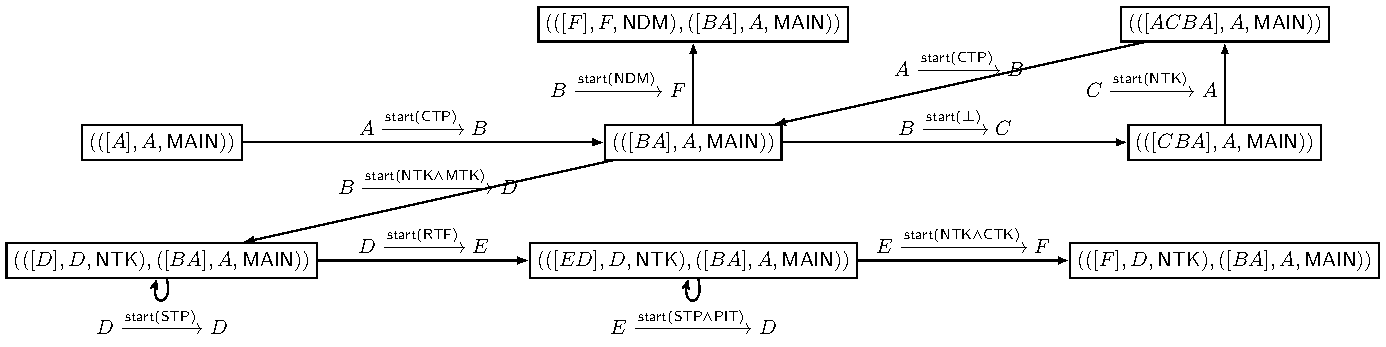
\includegraphics[scale = 0.63]{ifo-example.pdf}
        \caption{Configurations that are reachable from the initial configuration $(([A], A, \mainflag))$ in $\Mm$}
                %in $\phi$
        % \vspace{-6mm}	
        \label{ifo-example}
    \end{figure}
    
For instance,
        \begin{itemize}
        \item from the configuration $(([A], A, \mainflag))$, after executing the transition rule $A \xrightarrow{\startactivity(\ctpflag)} B$, because $\phi \models \neg \ntkflag \wedge \neg \ndmflag$, $B$ does not occur in the top task $[A]$, we have $\rho' = \push((([A], A, \mainflag)), B) = (([BA], A, \mainflag))$, 
		% moreover, $b' = \neg \nohflag$ since $\phi \not \models \nohflag$,
        %
        \item from the configuration $(([ACBA], A, \mainflag))$, after executing $A \xrightarrow{\startactivity(\ctpflag)} B$, because $\phi \models \neg \ntkflag \wedge \neg \ndmflag$, $B$ occurs in the top task $[ACBA]$, we have $\rho' = \clrtop((([ACBA], A, \mainflag)), B) = (([BA], A, \mainflag))$, 
		% moreover, $b' = \neg \nohflag$ since $\phi \not \models \nohflag$, 
 %resulting to the configuration $((([BA], A, \mainflag)),\neg \nohflag)$,
        %
	\item from the configuration $(([BA], A, \mainflag))$, after executing $B\xrightarrow{\startactivity(\bot)}C$, because $\phi\models\neg\ntkflag\wedge\neg\ndmflag\wedge\neg\ctpflag\wedge\neg\rtfflag\wedge\neg\stpflag$,and we have $\rho' = \push((([BA], A, \mainflag)), C) = (([CBA], A, \mainflag))$, 
	% moreover, $b' = \neg \nohflag$ since $\phi \not \models \nohflag$,
	%
	\item from the configuration $(([BA], A, \mainflag))$, after executing $B\xrightarrow{\startactivity(\ndmflag)}F$, because $\phi \models \ndmflag\wedge\neg\mtkflag$, $\getrealtsk(\rho,F) = *$,  we have 
	$\rho' = \newtsk((([BA], A, \mainflag)), F, \ndmflag) = (([F], F, \ndmflag),([BA], A, \mainflag))$, 
	% moreover, $b' = \nohflag$ since $\phi \models \nohflag$,
	%
		\item from the configuration $(([BA], A, \mainflag))$, after executing $B\xrightarrow{\startactivity(\ntkflag\wedge\mtkflag)}D$, because $\phi\models\ntkflag\wedge\neg\ndmflag\wedge\mtkflag$, we have 
		$$\rho' = \newtsk((([BA], A, \mainflag)), D, \ntkflag) = (([D],D,\ntkflag),([BA], A, \mainflag)),$$ 
	% moreover, $b' = \neg \nohflag$ since $\phi \not \models \nohflag$,
        %
        \item from the configuration $(([CBA], A, \mainflag))$, after executing $C \xrightarrow{\startactivity(\ntkflag)} A$, because 
        $\phi\models\ntkflag\wedge\neg\ndmflag\wedge\neg\mtkflag\wedge\neg\ctpflag\wedge\neg\rtfflag\wedge\neg\stpflag$, $\getrealtsk(\rho,A) = S_1$, $\zeta_1 = \mainflag$, we have 
		$$\rho' = \push((([CBA], A, \mainflag)), A) = (([ACBA], A, \mainflag)),$$
		%  moreover, $b' = \neg \nohflag$ since $\phi \not \models \nohflag$,
        %
        \item from the configuration $(([D],D,\ntkflag),([BA], A, \mainflag))$,  after executing  $D \xrightarrow{\startactivity(\stpflag)} D$, because $\phi \models \neg \ntkflag \wedge \neg \ndmflag\wedge\neg\ctpflag\wedge\neg\rtfflag\wedge\stpflag$ and $D$ is the top activity of the top task $[D]$, we have $\rho' = \rho$,
        %
        \item from the configuration $(([D],D,\ntkflag),([BA], A, \mainflag))$, after executing $D \xrightarrow{\startactivity(\rtfflag)} E$, because $\phi \models \neg \ntkflag \wedge \neg \ndmflag\wedge\neg\ctpflag\wedge\rtfflag$ and $E$ dose not occur in the top task $[D]$, we have 
		$$\rho' = \push((([D],D,\ntkflag),([BA], A, \mainflag)), E) = (([ED],D,\ntkflag),([BA], A, \mainflag)),$$
		% moreover, $b' = \neg \nohflag$ since $\phi \not \models \nohflag$,
        %
        \item from the configuration $(([ED],D,\ntkflag),([BA], A, \mainflag))$, after executing $E \xrightarrow{\startactivity(\stpflag\wedge\pitflag)} D$, because $\phi \models \neg \ntkflag \wedge \neg \ndmflag\wedge\neg\ctpflag\wedge\neg\rtfflag\wedge\stpflag\wedge\pitflag$ and $D = \preact([ED])$, we have $\rho' = \rho$, 
        %
        \item from the configuration $(([ED],D,\ntkflag),([BA], A, \mainflag))$, after executing $E \xrightarrow{\startactivity(\ntkflag\wedge\ctkflag)} F$,  because $\phi \models \ntkflag \wedge \neg \ndmflag\wedge\neg\mtkflag\wedge\ctkflag$, $\getrealtsk(\rho,F) = *$ and $\gettsk(\rho,F) = S_1$, we have 
		$$\rho' = \clrtsk((([ED],D,\ntkflag),([BA], A, \mainflag)), F) = (([F],D,\ntkflag),([BA], A, \mainflag)),$$
		%  moreover, $b' = \neg \nohflag$ since $\phi \not \models \nohflag$,
        %
\end{itemize}
\hide{
        \begin{itemize}
        \item from the configuration $((([A], A, \mainflag)), \neg \nohflag)$, after executing the transition rule $A \xrightarrow{\startactivity(\ctpflag)} B$, because $\phi \models \neg \ntkflag \wedge \neg \ndmflag$, $B$ does not occur in the top task $[A]$, $b = \neg \nohflag$, we have $\rho' = \push((([A], A, \mainflag)), B) = (([BA], A, \mainflag))$, moreover, $b' = \neg \nohflag$ since $\phi \not \models \nohflag$,
        %
        \item from the configuration $((([ACBA], A, \mainflag)), \neg \nohflag)$, after executing $A \xrightarrow{\startactivity(\ctpflag)} B$, because $\phi \models \neg \ntkflag \wedge \neg \ndmflag$, $B$ occurs in the top task $[ACBA]$, $b = \neg \nohflag$, we have $\rho' = \clrtop((([ACBA], A, \mainflag)), B) = (([BA], A, \mainflag))$, moreover, $b' = \neg \nohflag$ since $\phi \not \models \nohflag$, 
 %resulting to the configuration $((([BA], A, \mainflag)),\neg \nohflag)$,
        %
	\item from the configuration $((([BA], A, \mainflag)),\neg \nohflag)$, after executing $B\xrightarrow{\startactivity(\bot)}C$, because $\phi\models\neg\ntkflag\wedge\neg\ndmflag\wedge\neg\ctpflag\wedge\neg\rtfflag\wedge\neg\stpflag$,and $b=\neg\nohflag$, we have $\rho' = \push((([BA], A, \mainflag)), C) = (([CBA], A, \mainflag))$, moreover, $b' = \neg \nohflag$ since $\phi \not \models \nohflag$,
	%
	\item from the configuration $((([BA], A, \mainflag)),\neg \nohflag)$, afte executing $B\xrightarrow{\startactivity(\nohflag)}F$, because $\phi\models\neg\ntkflag\wedge\neg\ndmflag\wedge\neg\ctpflag\wedge\neg\rtfflag\wedge\neg\stpflag$, and $b = \neg\nohflag$, we have $\rho' = \push((([BA], A, \mainflag)), F) = (([FBA], A, \mainflag))$, moreover, $b' = \nohflag$ since $\phi \models \nohflag$,
	%
		\item from the configuration $((([BA], A, \mainflag)),\neg \nohflag)$, after executing $B\xrightarrow{\startactivity(\ntkflag\wedge\mtkflag)}D$, because $\phi\models\ntkflag\wedge\neg\ndmflag\wedge\mtkflag$ and $b = \neg\nohflag$, we have 
		$$\rho' = \newtsk((([BA], A, \mainflag)), D, \ntkflag) = (([D],D,\ntkflag),([BA], A, \mainflag)),$$ 
	moreover, $b' = \neg \nohflag$ since $\phi \not \models \nohflag$,
        %
        \item from the configuration $((([CBA], A, \mainflag)), \neg \nohflag)$, after executing $C \xrightarrow{\startactivity(\ntkflag)} A$, because $\phi\models\ntkflag\wedge\neg\ndmflag\wedge\neg\mtkflag\wedge\neg\ctpflag\wedge\neg\rtfflag\wedge\neg\stpflag$, $\getrealtsk(\rho,A) = S_1$, $\zeta_1 = \mainflag$, and $b = \neg \nohflag$, we have 
		$$\rho' = \push((([CBA], A, \mainflag)), A) = (([ACBA], A, \mainflag)),$$
		 moreover, $b' = \neg \nohflag$ since $\phi \not \models \nohflag$,
        %
        \item from the configuration $((([D],D,\ntkflag),([BA], A, \mainflag)),\neg\nohflag)$,  after executing  $D \xrightarrow{\startactivity(\stpflag)} D$, because $\phi \models \neg \ntkflag \wedge \neg \ndmflag\wedge\neg\ctpflag\wedge\neg\rtfflag\wedge\stpflag$ and $D$ is the top activity of the top task $[D]$, we have $(\rho',b') = (\rho,b)$,
        %
        \item from the configuration $((([D],D,\ntkflag),([BA], A, \mainflag)),\neg\nohflag)$, after executing $D \xrightarrow{\startactivity(\rtfflag)} E$, because $\phi \models \neg \ntkflag \wedge \neg \ndmflag\wedge\neg\ctpflag\wedge\rtfflag$ and $E$ dose not occur in the top task $[D]$, we have 
		$$\rho' = \push((([D],D,\ntkflag),([BA], A, \mainflag)), E) = (([ED],D,\ntkflag),([BA], A, \mainflag)),$$
		moreover, $b' = \neg \nohflag$ since $\phi \not \models \nohflag$,
        %
        \item from the configuration $((([ED],D,\ntkflag),([BA], A, \mainflag)),\neg\nohflag)$, after executing $E \xrightarrow{\startactivity(\stpflag\wedge\pitflag)} D$, because $\phi \models \neg \ntkflag \wedge \neg \ndmflag\wedge\neg\ctpflag\wedge\neg\rtfflag\wedge\stpflag\wedge\pitflag$ and $D = \preact([ED])$, we have $(\rho',b') = (\rho,b)$, 
        %
        \item from the configuration $((([ED],D,\ntkflag),([BA], A, \mainflag)),\neg\nohflag)$, after executing $E \xrightarrow{\startactivity(\ntkflag\wedge\ctkflag)} G$,  because $\phi \models \ntkflag \wedge \neg \ndmflag\wedge\neg\mtkflag\wedge\ctkflag$, $\getrealtsk(\rho,G) = *$ and $\gettsk(\rho,G) = S_1$, we have 
		$$\rho' = \clrtsk((([ED],D,\ntkflag),([BA], A, \mainflag)), G) = (([G],D,\ntkflag),([BA], A, \mainflag)),$$
		 moreover, $b' = \neg \nohflag$ since $\phi \not \models \nohflag$,
        %
        \item from the configuration $((([FBA], A, \mainflag)),\nohflag)$, after executing $F \xrightarrow{\startactivity(\ndmflag)} G$, because $\phi \models \ndmflag\wedge\neg\mtkflag\wedge\ctkflag$, $\getrealtsk(\rho,G) = *$, and $b = \nohflag$,  we have 
		$$\rho' = \rmact(\newtsk((([FBA], A, \mainflag)),G,\ndmflag),2,1) = (([G],G,\ndmflag),([BA], A, \mainflag)),$$ 
		moreover, $b' = \neg \nohflag$ since $\phi \not \models \nohflag$.
\end{itemize}
}
%    
\end{example}

The aforementioned informal description of intent flags and the example %enable us to 
provide the intuition of %understand 
the semantics of $\IFAOAMASS$. 
In the sequel, we formally define the semantics of $\Mm$ as a transition relation $\rho \xrightarrow[\tau]{\Mm} \rho'$ with $\tau = A \xrightarrow{\startactivity(\phi)} B$.

Let us assume $\phi \models \neg \tohflag$ first.

\smallskip

%We are ready to define the semantics of $\IFAOAMASS$. 
%The semantics of the transition rule $\back$ is similar to that of $\LMAOAMASS$. 
%Let us focus on the transition rules $A \xrightarrow{\startactivity(\phi)} B$. 

%\jinlong{omit $\nohflag$ here, and give an intuition of the $\nohflag$, the details defined in Appendix~\ref{app-ifaoamass}.}

%It turns out that the flag $\nohflag$ makes the definition of the semantics tedious. For instance, if the current top activity of the top task is started with the flag $\nohflag$, then it should be removed if it is not the top activity of the top task anymore after the application of a transition rule. To ease the understanding, we omit the flag $\nohflag$ first, and give a intuition of the semantics of $\Mm$ with $\nohflag$ later, the details of the formal semantics of $\Mm$ is defined in Appendix~\ref{app-ifaoamass}.
%Moreover we can largely reuse the definition of semantics of the case $\phi\models\neg\tohflag$. 
% Therefore, we assume that $\phi \models \neg \tohflag \wedge \neg \nohflag$ and $b = \neg \nohflag$ first. 
% in the sequel, we present the full semantics for the situation $b = \neg \nohflag$, but only illustrates the semantics partially for the situation $b =  \nohflag$ and delegate the full semantics to Appendix~\ref{app-sem-ifaoamass}.
% We first assume that $\phi \models \neg \tohflag \wedge \neg \nohflag$. We will consider $\phi \models \tohflag$ and $\phi \models \nohflag$ in the end. 
%In the sequel, $\nohflag$ is ignored first, and we distinguish two subcases, i.e., $\phi \models \neg \tohflag$ and $\phi \models \tohflag$.

%Let us define the semantics of $\Mm$ by a relation 
% $\rho \xrightarrow[\Mm]{\startactivity(\phi)} \rho'$ with $\phi \models \neg \tohflag \wedge \neg \nohflag$.
%$\rho \xrightarrow[\tau]{\Mm} \rho'$ with $\tau = A \xrightarrow{\startactivity(\phi)} B$.
%Let us consider the subcase $\phi \models \neg \tohflag$ first.

\noindent \fbox{$\phi \models \neg \ntkflag\wedge\neg\ndmflag$}
	\begin{itemize}
		\item If $\phi \models \ctpflag$ and $B \in \toptsk(\rho)$, then $\rho' = \clrtop(\rho, B)$.
		\item If $\phi \models \ctpflag$ and $B \notin \toptsk(\rho)$, then $\rho' = \push(\rho, B)$.
		\item If $\phi \models \neg \ctpflag$, then
		\begin{itemize}
			\item if $\phi \models \rtfflag$ and $B \in \toptsk(\rho)$, then $\rho'= \mvacttop(\rho, B)$, 
			\item if $\phi \models \rtfflag$ and $B \notin \toptsk(\rho)$, then $\rho' = \push(\rho, B)$, 
			\item if $\phi \models \neg \rtfflag$, then
			\begin{itemize}
				\item if $\phi \models \stpflag$ and $\topact(\rho) = B$ or $\phi \models \stpflag\wedge\pitflag$ and $\preact(\rho) = B$, then $\rho' = \rho$,
				\item otherwise, $\rho' = \push(\rho, B)$.
			\end{itemize}
		\end{itemize}
\end{itemize}

% 
\noindent \fbox{$\phi \models \ndmflag$}

\begin{itemize}
    \item If $\phi \models \mtkflag$, then $\rho'=\newtsk(\rho, B, \ndmflag)$.
    %
    \item If $\phi \models \neg \mtkflag$, then
   \begin{itemize}
        \item if $\getrealtsk(\rho, B) = S_i$, then
		\begin{itemize}
			\item if $\phi \models \ctkflag$, then $\rho' = \clrtsk(\mvtsktop(\rho, i), B)$,
			\item if $\phi \models \neg \ctkflag$, then
			\begin{itemize}
				\item if $B\in S_i$, then $\rho' = \clrtop(\mvtsktop(\rho, i), B)$,
				\item if $B\notin S_i$, then $\rho' = \push(\mvtsktop(\rho, i), B)$,
			\end{itemize}
		\end{itemize}
        \item if $\getrealtsk(\rho, B) = *$, then $\rho' = \newtsk(\rho, B, \ndmflag)$.
	\end{itemize}
\end{itemize}

% 
\smallskip
\noindent \fbox{$\phi \models \ntkflag \wedge \neg \ndmflag$}

\begin{itemize}
\item If $\phi \models \mtkflag$,  then $\rho' = \newtsk(\rho, B, \ntkflag)$.
%
\item If $\phi \models \neg \mtkflag$,  then
	\begin{itemize}
        \item if $\getrealtsk(\rho, B) = S_i$ or $\getrealtsk(\rho,B) = * \wedge\gettsk(\rho,B) = S_i$, then
		\begin{itemize}
			\item if $\phi \models \ctkflag$, then $\rho'=\clrtsk(\mvtsktop(\rho, i), B)$,
			\item if $\phi \models \neg \ctkflag$, then
			\begin{itemize}
				\item if $\phi \models \ctpflag$ and $B \in S_i$, then 
				$\rho'=\clrtop(\mvtsktop(\rho, i), B)$,
				\item if $\phi \models \ctpflag$ and $B \notin S_i$, then 
				$\rho'=\push(\mvtsktop(\rho, i), B)$,
				\item if $\phi \models \neg \ctpflag$, then
				\begin{itemize}
					\item if $\phi \models \rtfflag$ and $B \in S_i$, then
				$\rho'=\mvacttop(\mvtsktop(\rho, i), B)$,
					\item if $\phi \models \rtfflag$ and $B \notin S_i$, then
				$\rho'=\push(\mvtsktop(\rho, i), B)$,
					\item if $\phi \models \neg \rtfflag$, then
					\begin{itemize}
						\item if $\getrealtsk(\rho, B) = S_i$ and $\zeta_i \neq \mainflag$, 
						then $\rho' = \mvtsktop(\rho, i)$,
						\item otherwise, 
						\begin{itemize}
							\item if $\phi \models \stpflag$ and $\topact(S_i) = B$, or $\phi \models \stpflag \wedge \pitflag$ and $i = 1$ and $\preact(S_1) = B$, then $\rho' = \mvtsktop(\rho, i)$,
							\item otherwise, $\rho'=\push(\mvtsktop(\rho, i), B)$,
						\end{itemize}
					\end{itemize}
				\end{itemize}
			\end{itemize}
		\end{itemize}
	    %
	\item if $\gettsk(\rho, B) = *$, then $\rho' = \newtsk(\rho, B, \ntkflag)$.
	\end{itemize}
\end{itemize}

Finally we consider the situation $\phi \models \tohflag$.
% and $\nohflag$ is still ignored.
Let $\phi'$ be obtained from $\phi$ by replacing $\tohflag$ with $\neg \tohflag$. Moreover, 
suppose $\rho \xrightarrow [\tau']{\Mm} \rho'$, where $\tau' = A \xrightarrow{\startactivity(\phi')} B$ and $\rho' = (\Omega_1, \cdots, \Omega_{n})$. 
% suppose $(\rho, b) \xrightarrow [\startactivity(\phi')]{\Mm} (\rho', b')$, where $\rho' = (\Omega_1, \cdots, \Omega_{n})$. 
Then
\begin{itemize}
\item if $\phi \models \ntkflag \vee \ndmflag$, then let $\rho'' = (\Omega_1)$ and we have $\rho \xrightarrow [\tau]{\Mm} \rho''$,
%
\item otherwise, $\rho \xrightarrow [\tau]{\Mm} \rho'$.
\end{itemize}


%%%%%%%%%%%%%%%%%%%%%move to the appendix%%%%%%%%%%%%%%%%%%%
%%%%%%%%%%%%%%%%%%%%%move to the appendix%%%%%%%%%%%%%%%%%%%
\hide{
At last, let us consider the semantics of $\Mm$ with $\nohflag$. Firstly, we need adapt the concept of configurations as follows:
A configuration of $\Mm$ is encoded as a pair $(\rho, b)$, where $b \in \{\nohflag, \neg \nohflag\}$. Intuitively, $b$ denotes whether the topmost activity is started with $\nohflag$ or not.

% Now let us define the semantics of $\Mm$ by a relation $(\rho,b)\xrightarrow[\tau]{\Mm}(\rho',b')$ with $\tau = A\xrightarrow{\startactivity(\phi)}B$.
% Let $\phi'$ be obtained from $\phi$ by replacing $\nohflag$ with $\neg \nohflag$. Moreover, 
Suppose $\rho \xrightarrow [\tau]{\Mm} \rho'$.
Intuitively, $(\rho,b)\xrightarrow[\tau]{\Mm} (\rho'', b')$ is defined as follows:
\begin{itemize}
	\item If $b = \neg\nohflag$, then $\rho'' = \rho'$ 
	\begin{itemize}
		\item if $\phi \models \nohflag$, and the top activity of the top task in $\rho'$ is a fresh activity, then $b' = \nohflag$,
		\item otherwise, $b' = \neg \nohflag$.
	\end{itemize}
	\item If $b = \nohflag$, then
	\begin{itemize}
		\item if the top activity of the top task in $\rho$ is still the top activity of the top task in $\rho''$, then $\rho'' = \rho'$ and $b' = b$.
		\item otherwise, $\rho''$ is obtained from $\rho'$ by removing the original top activity of the top task in $\rho$, moreover,
		\begin{itemize}
			\item if $\phi \models \nohflag$, and the top activity of the top task in $\rho'$ is a fresh activity, then $b' = \nohflag$,
			\item otherwise, $b' = \neg \nohflag$.
		\end{itemize}
	\end{itemize}
\end{itemize}

% \noindent\emph{Case: $\alpha = \finishstart$}

% Similarly, let $\tau' = A\xrightarrow{\startactivity(\phi)}B$ and $\rho\xrightarrow[\tau']{\Mm}\rho''$ with $\rho''=((S_1',A_1',b_1'),\cdots,(S_{n'}',A_{n'}',b_{n'}'))$.
% \begin{itemize}
%     \item If $A_1\neq A_1'$, it means that the $A_1'$-task is the top task instead of $A_1$-task, hence $A$ is the top activity of $S_2'$, then $\rho' = \rmact(\rho'',2,1)$.
%     \item If $A_1=A_1$, it means that $A_1$-task is still the top task.
%     \begin{itemize}
%         \item if $|S_1|>|S_1'|$, it means that $A$ has popped, then $\rho' = \rho''$,
%         \item if $|S_1|<|S_1'|$, it means that $A$ is the second to top activity of $S_1'$, then $\rho' = \rmact(\rho'',1,2)$,
%         \item if $|S_1|=|S_1'|$, it means that $A$ is the top activity of $S_1'$, then $\rho' = \rmact(\rho'',1,1)$.
%     \end{itemize}
% \end{itemize}

Finally, let us consider the transition rules $A \xrightarrow{\finishstart(\phi)} B$. 
Intuitively, for a configuration $(\rho, b)$, $A \xrightarrow{\finishstart(\phi)} B$ will first start the activity $B$ with the intent flags specified by $\phi$,  then remove the original top activity $A$.
The definition of the semantics of $A \xrightarrow{\finishstart(\phi)} B$ is somehow similar to the semantics of $A \xrightarrow{\startactivity(\phi)} B$ on $(\rho, b)$ with $b = \nohflag$. The difference is that $A$ will always be removed for $A \xrightarrow{\finishstart(\phi)} B$, while this is not the case for $A \xrightarrow{\startactivity(\phi)} B$ and $b = \nohflag$. 
Since the formal semantics of $A \xrightarrow{\finishstart(\phi)} B$ is tedious, we omit it here and put it in Appendix~\ref{app-ifaoamass}. 
}
%%%%%%%%%%%%%%%%%%%%%move to the appendix%%%%%%%%%%%%%%%%%%%
%%%%%%%%%%%%%%%%%%%%%move to the appendix%%%%%%%%%%%%%%%%%%%


%The behavior $A \xrightarrow{\finishstart(\phi)} B$ is similar to $A \xrightarrow{\startactivity(\phi)} B$ and $b = \nohflag$. The difference is that $A$ will be terminated only if when $A$ is not the topmost activity of top task.

%The semantics of the transition rules $A \xrightarrow{\finishstart(\phi)} B$ is adapted from that for $A \xrightarrow{\startactivity(\phi)} B$ as follows:
%\begin{itemize}
%	\item remove the item and sub-items for the constraint $b = \neg\nohflag$,
%	\item replace $\rho' = \rho, b' = b$ with $\rho = \rmact(\rho, 1, 1), b' = \neg\nohflag$ for each item which contains $\rho' = \rho, b' = b$.
%\end{itemize}


By a retrospect of the aforementioned formal semantics, we can discover that the intent flags %are not independent of each other and they 
may interfere with each other. We summarize their dependencies as follows. 

\paragraph{Dependencies of intent flags.}
%Intuitively, for a transition $A\xrightarrow{\alpha(\phi)}B$, the intent flags in $\phi$ may depend on each other. 
The dependencies of intent flags can exhibit in the following two forms: (1) $n$ \emph{subsumes} $n'$, i.e., $n'$ is ignored if $n$ co-occurs with $n'$, and the ``subsume'' relations are transitive, (2) $n$ \emph{enables} $n'$, i.e., $n'$ takes effect if $n$ co-occurs with $n'$. The dependencies among the intent flags are summarized in Figure~\ref{fig-amass-depend}, where the solid lines represent the ``subsume'' relation, the dashed lines represent  the ``enable'' relation.
\begin{figure}[htbp]
    % \vspace{-3mm}
        \centering
        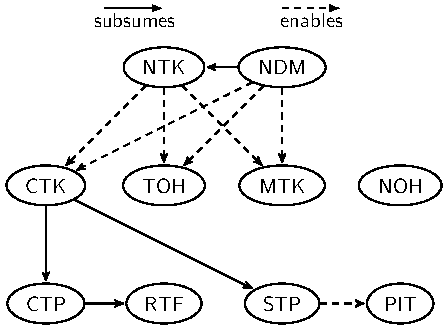
\includegraphics[scale = 0.7]{ifo-amass-dependency.pdf}
        \caption{Dependency graph of intent flags.}
            %in $\phi$
    % \vspace{-6mm}	
    \label{fig-amass-depend}
\end{figure}
\smallskip


\hide{
\smallskip
\noindent \fbox{$\phi \models \neg \ntkflag\wedge\neg\ndmflag$}
	\begin{itemize}
		\item If $\phi \models \ctpflag$ and $B \in \toptsk(\rho)$, then 
		\begin{itemize}
			\item if $\topact(\rho) \neq B$, then $\rho' = \clrtop(\rho, B)$, moreover, 
			\begin{itemize}
			\item if $\phi \models \neg \stpflag$, then $b' = \nohflag$ iff $\phi \models \nohflag$, 
			\item otherwise, $b' = \neg \nohflag$,
			\end{itemize}
			\item if $\topact(\rho) = B$, then $\rho' = \rho$, moreover,
			% $\rho' = \rho$, moreover,
			\begin{itemize}
			 	\item if $\phi \models \neg \stpflag$, then $b' = \nohflag$ iff $\phi \models \nohflag$, 
				\item otherwise, $b' = b$,
			\end{itemize}
		\end{itemize}
		\item If $\phi \models \ctpflag$ and $B \notin \toptsk(\rho)$, then $b' = \nohflag$ iff $\phi \models \nohflag$, moreover,
		\begin{itemize}
			\item if $b = \neg \nohflag$, then $\rho' = \push(\rho, B)$, 
			\item otherwise, $\rho' = \rmact( \push(\rho, B), 1, 2)$. 
		\end{itemize}
		\item If $\phi \models \neg \ctpflag$, then
		\begin{itemize}
			\item if $\phi \models \rtfflag$ and $B \in \toptsk(\rho)$, then
			\begin{itemize}
				\item if $\topact(\rho) \neq B$, then $b' = \neg \nohflag$, moreover, 
				\begin{itemize}
					\item if $b = \neg \nohflag$, then $\rho'= \mvacttop(\rho, B)$, 
					\item otherwise, $\rho' = \rmact(\mvacttop(\rho, B), 1, 2)$, 
				\end{itemize}
				\item if $\topact(\rho) = B$, then $\rho' = \rho$ and $b' = b$,
			\end{itemize}
			\item if $\phi \models \rtfflag$ and $B \notin \toptsk(\rho)$, then $b' = \nohflag$ iff $\phi \models \nohflag$, moreover,
			\begin{itemize}
				\item if $b = \neg \nohflag$, then $\rho' = \push(\rho, B)$, 
				\item otherwise, $\rho' = \rmact( \push(\rho, B), 1, 2)$. 
			\end{itemize}
			\item If $\phi \models \neg \rtfflag$, then
			\begin{itemize}
				\item if $\phi \models \stpflag$ and $\topact(\rho) = B$ or $\phi \models \stpflag\wedge\pitflag$ and $\preact(\rho) = B$, then $\rho' = \rho$ and $b' = b$,
				\item otherwise, $b' = \nohflag$ iff $\phi \models \nohflag$, moreover,
				\begin{itemize}
					\item if $b = \neg \nohflag$, then $\rho' = \push(\rho, B)$, 
					\item otherwise, $\rho' = \rmact( \push(\rho, B), 1, 2)$. 
				\end{itemize}
			\end{itemize}
		\end{itemize}
\end{itemize}

\smallskip
\noindent \fbox{$\phi \models \ndmflag$}

\begin{itemize}
    \item If $\phi \models \mtkflag$, then $b' = \nohflag$ iff $\phi  \models \nohflag$, 
    \begin{itemize}
    	\item if $b = \neg \nohflag$, then $\rho'=\newtsk(\rho, B, \ndmflag)$, 
	\item otherwise, $\rho'= \rmact(\newtsk(\rho, B, \ndmflag), 2, 1)$.
    \end{itemize}
    %
    \item If $\phi \models \neg \mtkflag$, then
   \begin{itemize}
        \item if $\getrealtsk(\rho, B) = S_i$, then
	\begin{itemize}
		\item if $i \neq 1$, then
        			\begin{itemize}
            			\item if $\phi \models \neg \ctkflag$, then 
				\begin{itemize}
					\item if $B \not \in S_i$, then $b' = \nohflag$ iff $\phi  \models \nohflag$, moreover, 
					\begin{itemize}
						\item if $b = \neg \nohflag$, then $\rho' = \push(\mvtsktop(\rho, i), B)$, 
						\item otherwise, $\rho' = \rmact(\push(\mvtsktop(\rho, i), B), 2, 1)$, 
					\end{itemize}
					\item otherwise, $b' = \neg \nohflag$,
					% \begin{itemize}
					% 	\item if $\phi \models \neg \stpflag$, then $b' = \nohflag$ iff $\phi  \models \nohflag$, 
					% 	\item otherwise, $b' = \neg \nohflag$, 
					% \end{itemize}
					moreover, 
					\begin{itemize}
						\item if $b = \neg \nohflag$, then $\rho'=\clrtop(\mvtsktop(\rho, i), B)$, 
						\item otherwise,  $\rho'= \rmact(\clrtop(\mvtsktop(\rho, i), B), 2, 1)$, 
					\end{itemize}
				\end{itemize}
            			\item if $\phi \models \ctkflag$, then $b' = \nohflag$ iff $\phi  \models \nohflag$, moreover, 
				\begin{itemize}
						\item if $b = \neg \nohflag$, then $\rho'=\clrtsk(\mvtsktop(\rho, i), B)$, 
						\item otherwise,  $\rho'= \rmact(\clrtsk(\mvtsktop(\rho, i), B), 2, 1)$, 
				\end{itemize}
        			\end{itemize}
		\item otherwise ($i = 1$), 
        			\begin{itemize}
            			\item if $\phi \models \neg \ctkflag$, then 
            			\begin{itemize}
					\item if $B \not \in S_1$, then $b' = \nohflag$ iff $\phi  \models \nohflag$, moreover, 
					\begin{itemize}
						\item if $b = \neg \nohflag$, then $\rho'=\push(\rho, B)$,
						\item otherwise, $\rho' = \rmact(\push(\rho, B), 1, 2)$,  
					\end{itemize}
            				\item if $B \in S_1$ and $\topact(S_1) \neq B$, then $\rho'= \clrtop(\rho, B)$ and $b' = \neg\nohflag$,
					% \begin{itemize}
					% 	\item if $\phi \models \stpflag$, then $b' = \neg \nohflag$, 
					% 	\item otherwise, $b' = \nohflag$ iff $\phi  \models \nohflag$,
					% \end{itemize}
					\item if $B \in S_1$ and $\topact(S_1) = B$ (this implies $A = B$), then $\rho' = \rho$ and $b' = b$,
			 	\end{itemize}
            			\item if $\phi \models \ctkflag$, then $\rho'= \clrtsk(\rho, B)$, and $b' = \nohflag$ iff $\phi  \models \nohflag$, 
				% \begin{itemize}
				% 	\item if $\phi \models \stpflag$, then $b' = \neg \nohflag$, moreover, 
				% 	\begin{itemize}
				% 		\item if $B \not \in S_1$, then 
				% 	\end{itemize}
				% 	\item otherwise, $b' = \nohflag$	iff $\phi  \models \nohflag$, 		
				% \end{itemize}
            	% 		\begin{itemize}
				% 	\item if $B \not \in S_1$, then $b' = \nohflag$ iff $\phi  \models \nohflag$, moreover, 
				% 	\begin{itemize}
				% 		\item if $b = \neg \nohflag$, then $\rho' = \push(\rho, B)$,
				% 		\item otherwise, $\rho' = \rmact(\push(\rho, B), 1, 2)$, 
				% 	\end{itemize}
            	% 			\item if $B \in S_1$ and $\topact(S_1) \neq B$, then $\rho'= \clrtsk(\rho, B)$, moreover, $b' = \nohflag$ iff $\phi  \models \nohflag$, 
				% 	\item if $B \in S_1$ and $\topact(S_1) = B$ (this implies $A = B$), then $\rho'= \rho$ and $b' = b$,
			 	% \end{itemize}
        			\end{itemize}
	\end{itemize}
        \item if $\getrealtsk(\rho,B) = *$, then  $b' = \nohflag$ iff $\phi \models \nohflag$, moreover,
        \begin{itemize}
        		\item if $b = \neg \nohflag$, then $\rho'=\newtsk(\rho, B, \ndmflag)$, 
		\item otherwise, $\rho'=\rmact(\newtsk(\rho, B, \ndmflag), 2, 1)$.
        \end{itemize}
    \end{itemize}
\end{itemize}    

\smallskip
\noindent \fbox{$\phi \models \ntkflag \wedge \neg \ndmflag$}

\begin{itemize}
\item If $\phi \models \mtkflag$,  then $b' = \nohflag$ iff $\phi \models \nohflag$, moreover, 
	\begin{itemize}
		\item if $b = \neg \nohflag$, then $\rho' = \newtsk(\rho, B, \ntkflag)$, 
		\item otherwise, $\rho' = \rmact(\newtsk(\rho, B, \ntkflag), 2, 1)$.
	\end{itemize}
%
\item If $\phi \models \neg \mtkflag$,  then
	\begin{itemize}
        \item if $\getrealtsk(\rho, B) = S_i$ or $\getrealtsk(\rho,B) = * \wedge\gettsk(\rho,B) = S_i$, then
        \begin{itemize}
        \item if $i \neq 1$, then 
			\begin{itemize}
				\item if $\phi \models \ctkflag$, then $b' = \nohflag$ iff $\phi \models \nohflag$, moreover, 
                \begin{itemize}
					\item if $b = \neg \nohflag$, then $\rho'=\clrtsk(\mvtsktop(\rho, i), B)$,
					\item otherwise, $\rho' = \rmact(\clrtsk(\mvtsktop(\rho, i), B), 2, 1)$, 
                \end{itemize}
				\item if $\phi \models \neg \ctkflag$, then
					\begin{itemize}
						\item if $\phi \models\ctpflag$ and $B \in S_i$, then 
						\begin{itemize}
							\item if $b = \neg \nohflag$, then $\rho'=\clrtop(\mvtsktop(\rho, i), B)$,
							\item otherwise, $\rho' = \rmact(\clrtop(\mvtsktop(\rho, i), B), 2, 1)$, 
						\end{itemize}
						moreover, 
						\begin{itemize}
							\item if $\phi\models \neg \stpflag$, then $b' = \nohflag$ iff $\phi \models \nohflag$, 
							\item otherwise $b' = \neg \nohflag$, 
						\end{itemize}
						\item if $\phi \models\ctpflag$ and $B \notin S_i$, then $b' = \nohflag$ iff $\phi \models \nohflag$, moreover, 
						\begin{itemize}
							\item if $b = \neg \nohflag$, then $\rho'=\push(\mvtsktop(\rho, i), B)$,
							\item otherwise, $\rho' = \rmact(\push(\mvtsktop(\rho, i), B), 2, 1)$, 
						\end{itemize}
						\item if $\phi \models\neg\ctpflag$, then
						\begin{itemize}
							\item if $\phi \models \rtfflag$ and $B\in S_i$, then $b' = \neg \nohflag$, moreover,
							\begin{itemize}
								\item if $b = \neg \nohflag$, then $\rho'=\mvacttop(\mvtsktop(\rho, i), B)$,
								\item otherwise, $\rho' = \rmact(\mvacttop(\mvtsktop(\rho, i), B), 2, 1)$, 
							\end{itemize}
							\item if $\phi \models \rtfflag$ and $B\notin S_i$, then $b' = \nohflag$ iff $\phi \models \nohflag$, moreover, 
							\begin{itemize}
								\item if $b = \neg \nohflag$, then $\rho'=\push(\mvtsktop(\rho, i), B)$,
								\item otherwise, $\rho' = \rmact(\push(\mvtsktop(\rho, i), B), 2, 1)$, 
							\end{itemize}
							\item if $\phi \models \neg \rtfflag$, then
							\begin{itemize}
								\item if $\getrealtsk(\rho,B) = S_i$ and $\zeta_i \neq \mainflag$, then $b' = \neg \nohflag$, moreover,
								\begin{itemize}
									\item if $b = \neg \nohflag$, then $\rho'=\mvtsktop(\rho, i)$,
									\item otherwise, $\rho' = \rmact(\mvtsktop(\rho, i), 2, 1)$, 
								\end{itemize}
								\item otherwise ($\getrealtsk(\rho,B) = S_i$ and $\zeta_i = \mainflag$ or $\getrealtsk(\rho,B) = * \wedge\gettsk(\rho,B) = S_i$), 
								\begin{itemize}
									\item if $\phi\models\stpflag$ and $\topact(S_i) = B$, then $b' = \neg \nohflag$, moreover,
									\begin{itemize}
										\item if $b = \neg \nohflag$, then $\rho'=\mvtsktop(\rho, i)$,
										\item otherwise, $\rho' = \rmact(\mvtsktop(\rho, i), 2, 1)$, 
									\end{itemize}
									\item otherwise, $b' = \nohflag$ iff $\phi \models \nohflag$, moreover, 
									\begin{itemize}
										\item if $b = \neg \nohflag$, then $\rho'=\push(\mvtsktop(\rho, i), B)$,
										\item otherwise, $\rho' = \rmact(\push(\mvtsktop(\rho, i), B), 2, 1)$, 
									\end{itemize}
								\end{itemize}
							\end{itemize}
						\end{itemize}
					\end{itemize}
			\end{itemize}
		\item otherwise ($i  = 1$),  
		\begin{itemize}
			\item if $\phi \models \ctkflag$, then $\rho' = \clrtsk(\rho,B)$ and $b' = \nohflag$ iff $\phi \models \nohflag$, 
			\item if $\phi \models \neg \ctkflag$, then
			\begin{itemize}
				\item if $\phi \models \ctpflag$ and $B \in S_1$, then $\rho'=\clrtop(\rho, B)$, moreover, 
%				\begin{itemize}
%					\item if $\phi\models \neg \stpflag$, then $b' = \nohflag$ iff $\phi \models \nohflag$, 
%					\item otherwise, $b' = \neg \nohflag$,
%				\end{itemize}
				\begin{itemize}
            				\item if $A \neq B$, then $\rho'=\clrtop(\rho, B)$, moreover, 
					\begin{itemize}
						\item if $\phi\models \neg \stpflag$, then $b' = \nohflag$ iff $\phi \models \nohflag$, 
						\item otherwise, $b' = \neg \nohflag$, 
					\end{itemize}
					\item if $A = B$, 
					% then $\rho' = \rho$, moroever,  
					\begin{itemize}
						\item if $\phi \models \neg \stpflag$, then $\rho' = \clrtop(\rho, B)$ and $b' = \nohflag$ iff $\phi \models \nohflag$, 
						\item otherwise, $\rho' = \rho$ and $b' = b$,
					\end{itemize}
				\end{itemize}
				\item if $\phi \models \ctpflag$ and $B\notin S_1$, then $b' = \nohflag$ iff $\phi \models \nohflag$, moreover,
				\begin{itemize}
					\item if $b = \neg \nohflag$, then $\rho'=\push(\rho, B)$,
					\item otherwise, $\rho' = \rmact(\push(\rho, B), 1, 2)$, 
				\end{itemize}
				\item if $\phi \models \neg \ctpflag$, then
				\begin{itemize}
					\item if $\phi \models \rtfflag$ and $B \in S_1$, then
					\begin{itemize}
                					\item if $A \neq B$, then $b' = \neg \nohflag$, moreover, 
                					\begin{itemize}
                						\item if $b = \neg \nohflag$, then $\rho'=\mvacttop(\rho, B)$,
							\item otherwise, $\rho' = \rmact(\mvacttop(\rho, B), 1, 2)$,
						\end{itemize}
                					\item if $A = B$, then $\rho' = \rho$ and $b' = b$, 
                				\end{itemize}
					\item if $\phi \models \rtfflag$ and $B \notin S_1$, then $b' = \nohflag$ iff $\phi \models \nohflag$, moreover,
					\begin{itemize}
						\item if $b = \neg \nohflag$, then $\rho'=\push(\rho, B)$,
						\item otherwise, $\rho' = \rmact(\push(\rho, B), 1, 2)$, 
					\end{itemize}
					\item if $\phi \models \neg \rtfflag$, then
					\begin{itemize}
						\item if $\getrealtsk(\rho,B) = S_1$ and $\zeta_1 \neq \mainflag$, then $\rho' = \rho$ and $b' = b$,
						\item otherwise ($\getrealtsk(\rho,B) = S_1$ and $\zeta_i = \mainflag$ or $\getrealtsk(\rho,B) = * \wedge\gettsk(\rho,B) = S_1$), 
						\begin{itemize}
							\item if $\phi\models\stpflag$ and $A = B$, or $\phi \models\stpflag\wedge\pitflag$ and $\preact(\rho) = B$, then $\rho' = \rho$ and $b' = b$, 
							\item otherwise, $b' = \nohflag$ iff $\phi \models \nohflag$, moreover, 
							\begin{itemize}
								\item if $b = \neg \nohflag$, then $\rho'=\push(\rho, B)$,
								\item otherwise, $\rho' = \rmact(\push(\rho, B), 1, 2)$, 
							\end{itemize}
						\end{itemize}
					\end{itemize}
				\end{itemize}
			\end{itemize}
		\end{itemize}
	\end{itemize}
	    %
	\item if $\gettsk(\rho, B) = *$, then $b' = \nohflag$ iff $\phi \models \nohflag$, moreover, 
		\begin{itemize}
			\item if $b = \neg \nohflag$, then $\rho' = \newtsk(\rho, B, \ntkflag)$, 
			\item otherwise, $\rho' = \rmact(\newtsk(\rho, B, \ntkflag), 2, 1)$.
		\end{itemize}				
	\end{itemize}
\end{itemize}
}



%!TEX root = main.tex

%\revision{
\subsubsection{Semantics of $\FOAMASS$}\label{sec-foamass}
In this case, we assume that there is only one activity $A_0$ and consider the fragments as the atomic objects, hence we only consider the transaction rules $\back$ , $A\xrightarrow{\mu}T$ and $F\xrightarrow{\mu}T$, where $T$ is of the form $(\beta_1(F_1, i_1, x_1), \cdots, \beta_k(F_k, i_k, x_k))$ such that for every $j \in [k]$, $\beta_j \in \{\ADD, \REP, \REM\}$, $F_j \in \frag$, $i_j \in \Nn$, and $x_j$ is a variable storing the identifiers of fragment instances.
%}

\subsection*{Intuitions.}
The intuitions of the transition rules  $A\xrightarrow{\mu}T$ and $F\xrightarrow{\mu}T$ are explained in the sequel. 
\begin{itemize}
	\item 
	$\ADD(F, i,  x)$ denotes the action where a \emph{new} instance of the fragment $F$ is added to the container $i$ of the current activity. Moreover, the identifier of the new instance is stored in $x$.
	
	\item $\REP(F, i,  x)$ is the same as $\ADD(F, i,  x)$, except that the container %of identifier 
	$i$ is cleared before adding $F$. 
%
	\item $\REM(F, i,  x)$ denotes the action where the instance of the fragment $F$ of the identifier (stored in) $x$ is removed from the container $i$ of the current activity.	 
	
\item $\opstack[(\beta_1(F_1, i_1, x_1), \cdots, \beta_k(F_k, i_k, x_k))]$ denotes that the actions $\beta_1(F_1, i_1, x_1),\cdots, \beta_k(F_k, i_k, x_k)$ are executed sequentially, and %$(\beta_1(F_1, i_1), \cdots, \beta_k(F_k, i_k))$ is
	are added to the transaction stack. 
\item $\nopstack[(\beta_1(F_1, i_1, x_1), \cdots, \beta_k(F_k, i_k, x_k))]$ is the same as $\opstack$, except that %$(\beta_1(F_1, i_1), \cdots, \beta_k(F_k, i_k))$
	the transactions will \emph{not} be added to the transaction stack. \\
	For convenience, these transition rules are called $\opstack$-transition rules and $\nopstack$-transition rules respectively.
\end{itemize}

It is fair to say that the intricacy of the semantics lies in the action $\back$. Let $A$ be the top activity of the top task, %$\vgr(A)=(i_1, \cdots, i_m)$, and $\upsilon = ((V_1, i_1), \cdots, (V_m, i_m))$ be an enumeration of the fragment stacks corresponding to the containers (where $V_j \in \frag^*$ for every $j \in [m]$), 
$\vgr(A)=(i_1, \cdots, i_m)$, $V_{1}$, $\cdots$, $V_{m}$ be the fragment stacks for the containers $i_1, \cdots, i_m$,  
%where each $V_i$ is a fragment stack 
and $\eta \in \ops^*$ be the transaction stack. 
If $\eta = \epsilon$, the activity $A$ will be popped, otherwise the behavior of the action $\back$ is controlled by $\eta$, namely, when the back button is pressed, the top transaction of $\eta$ is removed from $\eta$ and its effects on the fragment stacks %$\upsilon$ are canceled
are to be revoked. Noticeable difficulties arise.  %Canceling the effects of an transaction is intricate in the following two aspects: 

\smallskip
\noindent\emph{Mismatch between fragment and transaction stack.} 
The transaction stack $\eta$ may \emph{not} contain all the historical transactions leading to the fragment stacks, but only those corresponding to the $\opstack$-transition rules, which means that when revoking the top action of $\eta$, say $\ADD(F, i_j, x_j)$, $F$ may not be the top fragment of $V_j$. To deal with this issue, we 
\begin{enumerate}
\item store $(F, n)$ in $V_{j}$, where $n$ is the identifier of the instance of $F$ which is generated when applying $\ADD(F, i_j, x_j)$,  
\item store the concretized action $\ADD(F, i_j, n)$, instead of $\ADD(F, i_j, x_j)$, into the transaction stack $\eta$.
\end{enumerate}
As a result, we can revoke $\ADD(F, i_j, n)$ instead of $\ADD(F, i_j, x_j)$ in the transaction stack, and use $n$ to identify the fragment instance to be removed from the fragment container $V_j$.
%
%Note that when revoking $\ADD(F, i_j, x_j)$, the variable $x_j$ cannot be used to find the fragment instance since $x_j$ since $x_j$ may have been reused to store the identifiers of the other fragment instances.

\smallskip
\noindent\emph{Revoking $\REP$ actions.} The top transaction of $\eta$ may include some action $\REP(F, i_j, n)$ and revoking these actions requires restoring the historical content of the container $i_j$ before applying this action.

%To deal with the first issue, %mismatch between $\upsilon$ and $\eta$, 
%when defining the formal semantics in the sequel, the tag $\sharp$ is used 
%we use a tag $\sharp$ to distinguish between the fragment instances added by the $\opstack$-transition rules and those added by the $\nopstack$-transition rules. When applicable, pairs $(F, \sharp)$, instead of fragments $F$,  are pushed into the fragment stack. %container.

%To deal with the second issue, %the canceling of $\REP$ actions, 
%we introduce a new action $\REM(F', i_j)$ where $F' \in \frag \cup (\frag \times \{\sharp\})$, whose meaning is to remove the topmost occurrence of $F'$ from the container $i_j$. 
%
To deal with this issue, 
when an action $\REP(F, i_j, x_j)$ appears in a $\opstack$-transition rule and is to be pushed into the transaction stack, suppose that the current content of the container $i_j$ is $((F'_1,n'_1),  \cdots, (F'_k, n'_k))$, then $\REP(F, i_j, x_j)$ is concretized into the action sequence 
$$\REM(F'_1, i_j, n'_1), \cdots, \REM(F'_k, i_j, n'_k), \ADD(F, i_j, n),$$ 
which---instead of $\REP(F, i_j, n)$---is pushed into the transaction stack, possibly together with the other actions in the same transaction. 
(Note that $n$ is the identifier of the newly created instance of $F$.)
Hence revoking $\REP(F, i_j, x_j)$ is to apply the concretized actions
%the inverse of the action sequence $\REM(F'_1, j), \cdots, \REM(F'_k, j), \ADD((F,\sharp), j)$, namely, 
$\REM(F, i_j, n), \ADD(F'_k, i_j, n'_k), \cdots, \ADD(F'_1, i_j, n'_1)$ one by one.

Therefore, only concretized actions of the form $\ADD(F, i, n)$ or $\REM(F, i, n)$ are stored in the transaction stack, and we use $\cops$ to denote the set of these concretized actions.  



\subsection*{Fragment containers and configurations.}
%
%Let $\frag^\sharp = \frag \times \{\sharp\}$. 
%,  where the tag $\sharp$ is introduced for encoding the semantics of the action $\back$ and will be explained later on.
 
A \emph{fragment \container} is encoded as 
$$V = ((F_1, n_1), \cdots, (F_k, n_k)) \in (\frag \times \Nn)^+ ,$$ where $n_j$ is the identifier of an instance of $F_j$ for $j \in [k]$ and $k$ is called the \emph{height} of $V$.

%
A \emph{configuration} $\rho$ %with {\container} $\vgr(A) = (V_1, \cdots, V_m)$ 
is encoded as a tuple $(\upsilon, \eta, \iota)$, where %$\upsilon = ((V_1, i_1), \cdots, (V_m, i_m))$ such that $V_j \in (\frag\cup \frag^{\sharp})^+$ is the corresponding fragment stack  to $i_j$, and 
$\upsilon = (V_1, \cdots, V_m)$  is a sequence of fragment containers associated with $A_0$, where $\vgr(A_0) = (i_1,\cdots,i_m)$, $\eta= (T_1, \cdots, T_n) \in \cops^*$ is the transaction stack, and $\iota$ is the assignment function that assigns to each variable $x$ in $\Mm$ an identifier, i.e. a natural number. Note that it is possible that $m=0$ and/or $n=0$. For technical convenience, let $\iota_0$ denote the assignment function that assigns each variable $x$ the value $0$. The initial configuration of $\Mm$ is $((\epsilon,\cdots,\epsilon),\epsilon,\iota_0)$.

%%%%%%%%%%%%%%%%%%%%%%%%%%%%%%%%%%%%%%%%%%%%%%%%%%%%%%%%%%%%%%%%%%
%%%%%%%%%%%%%%%%%%%%%%%%%%%%%%%%%%%%%%%%%%%%%%%%%%%%%%%%%%%%%%%%%%
\subsection*{Auxiliary functions and predicates.} To specify the transition relation precisely and concisely, we define the following functions and predicates. 
For a container $V=((F_1, n_1), \cdots, (F_{m}, n_m))$, define $\tfrag(V) = F_1$.
%For $\rho_v = (V_1,\dots,V_n)$, $\rho_o = (O_1,\dots,O_n)$, $\vec{\beta} = [\beta_1(F_1',V_1),\dots,\beta_m(F_m',V_m)]$
%\begin{itemize}
%	\item   $\tfrag(V) = F_1$,  
	%
%		\item $\getfrag(F, V) = \min\{1\leq i\leq m  \mid F = F_i\}$ and we write $\bot$ for $\min\emptyset$. $\getfrag(F, V)$ returns the first (topmost) instance of $F$ in $V$. 
		%otherwise, $\getfrag(F, V) = \bot$. (Intuitively, $\getfrag(F, V)$ returns the index of the first occurrence of $F$ in $V$.)
%	\item  If there is $i \in [m]$ such that $F = F_i$ and for every $ j \in [i-1], F_j \neq F$, then $\getfrag(F, V) = i$; otherwise, $\getfrag(F, V) = \bot$. (Intuitively, $\getfrag(F, V)$ returns the index of the first occurrence of $F$ in $V$.)
%\end{itemize}

Let $\rho = (\upsilon, \eta, \iota)$ be the configuration of associated with $A_0$, where $\vgr(A_0) = (i_1, \cdots, i_k)$  ($k > 0$), $\upsilon = (V_1, \cdots, V_k)$ is the container sequence, and $\eta = (T_1, \cdots, T_l)$ ($l \ge 0$) is the transaction stack. Moreover, let $F \in \frag$, $j \in [k]$, and $x$ be a variable. 
We define the following functions.

%Then we define the following functions manipulating containers.
%For $\rho_v = (V_1,\dots,V_n)$, $\rho_o = (O_1,\dots,O_n)$, $\vec{\beta} = [\beta_1(F_1',V_1),\dots,\beta_m(F_m',V_m)]$
\begin{itemize}
\item %For a container $V=(F'_1, \cdots, F'_{m'})$, define $\tfrag(V) = F'_1$. Moreover, 
$\tfrag(\upsilon) = \{\tfrag(V_i) \mid i \in [k], V_i \neq \epsilon\}$ returns the set of topmost fragments of containers in $\upsilon$.
%
%\item  For a container $V=(F'_1, \cdots, F'_{m'})$, define $\getfrag(F', V)$ as follows: If there is $i \in [m']$ such that $F' = F'_i$ and for every $ j \in [i-1], F'_j \neq F'$, then $\getfrag(F', V) = i$.
%        Otherwise, $\getfrag(F', V) = \bot$.
%
\item  $\ADD(F, i_j, x)(\upsilon, \iota) = (\upsilon', \iota')$, where $\upsilon' = (V_1, \cdots, V_{j-1}, (F, n) \cdot V_j, V_{j+1}, \cdots, V_k)$, $\iota' =\iota[n/x]$,  and $n$ is the \emph{minimum} identifier not occurring in $\upsilon$ or $\iota$. Intuitively, $\ADD(F, i_j, x)(\upsilon, \iota)$ updates $(\upsilon, \iota)$ by choosing a fresh identifier $n$, pushing $(F, n)$ into the container $i_j$, and storing $n$ into $x$. 
%    otherwise, 
%    $$(\ADD(F', i))(\upsilon) = (((F'), i'), (V_1, i_1), \cdots, (V_k, i_k)).$$
%
 \item $\REP(F, i_j, x)(\upsilon, \iota) =  (\upsilon', \iota')$, where $\upsilon' = (V_1, \cdots, V_{j-1}, (F, n), V_{j+1}, \cdots, V_k)$, $\iota' = \iota[n/x]$, and $n$ is the \emph{minimum} identifier not occurring in  $\upsilon$ or $\iota$. Intuitively, $\REP(F, i_j, x)(\upsilon, \iota)$ updates $\upsilon$ by replacing the content of container $i_j$ with $(F, n)$, and storing $n$ into $x$.
    %
%    otherwise, 
    %
%    $$(\REP(F',i'))(\upsilon) = (((F'), i'), (V_1, i_1), \cdots, (V_k, i_k)).$$
%
\item Suppose $V_j = ((F_1, n_1), \cdots, (F_{m}, n_m))$, then
%
$\REM(F, i_j, x)(\upsilon, \iota) = (\upsilon', \iota')$, 
%
where 
\begin{itemize}
\item $\upsilon' = (V_1, \cdots, V_{j-1}, \tilde{V}$, $V_{j+1}, \cdots, V_k)$ such that
\begin{itemize}
\item $\tilde{V} = V_j$,  if $\iota(x) \neq n_{j'}$ for every $j' \in [m]$, and 
\item $\tilde{V} = ((F_1,n_1), \dots, (F_{l-1}, n_{l-1}), (F_{l+1}, n_{l+1}), \dots, (F_{m}, n_m))$, if $\iota(x) = n_l$, 
\end{itemize}
\item moreover, $\iota' = \iota$.
\end{itemize}

Intuitively, the action $\REM(F, i_j, x)(\upsilon)$ updates $\upsilon$ by removing the instance of $F$ of the identifier $\iota(x)$ from container $i_j$ and does not change $\iota$.
%
\item Furthermore, the functions $\ADD(F, i_j, n)(\upsilon, \iota)$, $\REP(F, i_j, n)(\upsilon, \iota)$, $\REM(F, i_j, n)(\upsilon, \iota)$ for concretized actions can be defined similarly (except that $\iota$ is unchanged).
\end{itemize}

For a  transaction $T=(\beta_1(F_1, j_1, x_1), \cdots, \beta_{r}(F_r, j_r, x_r))$ such that $\beta_s \in \{\ADD,\REM,\REP\}$ and $F_s \in \frag$ for every $s \in [r]$, 
 $\updateviews_T(\upsilon, \iota)= (\upsilon_r, \iota_r)$, where $(\upsilon_0, \iota_0) = (\upsilon, \iota)$, and for every $s \in [r]$, $(\upsilon_s, \iota_s) = \beta_s(F_s, j_s, x_s)(\upsilon_{s-1}, \iota_{s-1})$, i.e. $\updateviews_T$ updates the containers and the assignment function by applying the actions in $T$. Furthermore, $\updateviews_T(\upsilon, \iota)$ can be defined similarly for concretized transactions $T$.


%\begin{itemize}
    %(Note in $O^{-1}$, the sequence $\beta_1, \cdots, \beta_r$ is reversed and $\sharp$ is added.)
    %
%    \item For an transaction $O=(\beta_1(F'_1, j_1), \cdots, \beta_{r}(F'_r, j_r))$ such that $\beta_s \in \{\ADD,\REM\}$ and $F'_s \in \frag \cup \frag^\sharp$ for every $s \in [r]$ (note here $\beta_s \neq \REP$), 
%    
  
%\item   $\updateviews_T(\upsilon, \iota)= (\upsilon_r, \iota_r)$, where $(\upsilon_0, \iota_0) = (\upsilon, \iota)$, and for every $s \in [r]$, $(\upsilon_s, \iota_s) = \beta_s(F_s, j_s)(\upsilon_{s-1}, \iota_{s-1})$, i.e. $\updateviews_T$ updates the containers and the assignment function by applying the actions in $T$, 
%
%\item if $F_1, \cdots, F_r \in \frag$, then $\updateviews^\sharp_T(\upsilon, \iota)= (\upsilon_r, \iota')$, where $\upsilon_0 = \upsilon$, and for every $s \in [r]$, 
%$(\upsilon_s, \iota_s) = \beta_s((F_s,\sharp), j_s)(\upsilon_{s-1}, \iota_{s-1})$, i.e. $\updateviews^\sharp_T$ updates the containers by applying the $\sharp$-decorated actions in $T$, 
%
%\item   $T^{-1} = (\beta^{-1}_r(F_r, j_r), \cdots, \beta^{-1}_{1}(F_1, j_1))$ is the dual transaction of $T$.
%\end{itemize}

We also introduce a function that concretize the actions $\REP$ by utilizing the containers in $\upsilon$. Suppose $F \in \frag$, $j \in [k]$, $x$ is a variable, and $V_j = ((F_1, n_1), \cdots, (F_{m}, n_m))$. Let $n$ be the minimum identifier not occurring in $\upsilon$ or $\iota$.
% \begin{itemize}
%\item 
Then
$$
%\begin{array}{l}
\concaction_{\upsilon, \iota}(\REP(F, i_j, x)) =
%\ \ \ \ 
\REM(F_{1}, i_j, n_1), \cdots, \REM(F_{m}, i_j, n_m), \ADD(F, i_j, n).
%\end{array}
$$
%where $n$ is the minimum identifier not occurring in $\Theta$.
%
%
Moreover, let 
$$\concaction_{\upsilon,\iota}(\ADD(F, i_j, x)) = \ADD(F, i_j, n) \mbox{ and } \concaction_{\upsilon,\iota}(\REM(F, i_j, x)) = \REM(F, i_j, \iota(x))$$
by convention.
%
%\item $\concaction^\sharp_\upsilon(\ADD(F, i_j))$ and $\concaction^\sharp_\upsilon(\REP(F, i_j))$ are defined similarly, with $F$ replaced by $(F, \sharp)$,
%

Let $T = (\beta_1(F_1, j_1, x_1), \cdots, \beta_k(F_r, j_r, x_r))$ be a transaction such that $\beta_s \in \{\ADD,\REM, \REP\}$, and $F_s \in \frag$ for every $s \in [r]$.
We define $\concaction_{\upsilon, \iota}(T)$ as the concatenation of the concretized action sequences 
$ \concaction_{\upsilon_0, \iota_0}(\beta_1(F_1, j_1, x_1))$, $\cdots$, $\concaction_{\upsilon_{s-1}, \iota_{s-1}}(\beta_s(F_s, j_s, x_s))$,
where $(\upsilon_0, \iota_0)= (\upsilon, \iota)$, and for each $s \in [r]$, $(\upsilon_s, \iota_s) = \beta_s(F_s, j_s, x_s)(\upsilon_{s-1}, \iota_{s-1})$.

Finally, we define functions $\beta^{-1}(F, i_j, n)$ for $\beta(F, i_j, n) \in \cops$ as follows.
\begin{itemize}
 \item $\ADD^{-1}(F, i_j, n)(\upsilon, \iota) =\REM(F, i_j, n)(\upsilon, \iota)$,
 \item $\REM^{-1}(F, i_j, n)(\upsilon, \iota) = \ADD(F, i_j, n)(\upsilon, \iota)$.
\end{itemize}
Intuitively, $\ADD(F, i_j, n)$ and $\REM(F, i_j, n)$ are dual actions.
%
Moreover, for a concretized transaction 
$$T = (\beta_1(F_1, j_1, n_1), \cdots, \beta_{r}(F_r, j_r, n_r))$$ 
such that $\beta_s \in \{\ADD,\REM,\REP\}$, $F_s \in \frag$ for every $s \in [r]$, and $n \in \Nn$, we define $T^{-1}$ as 
$$(\beta^{-1}_{r}(F_r, j_r, n_r), \cdots, \beta^{-1}_1(F_1, j_1, n_1)).$$



%===============================================================================================================	
\subsection*{Transition relation.} 
We assume that the current activity is $A$. For $\rho\xrightarrow[\tau]{\Mm}\rho'$, we let $\rho = (\upsilon,\eta,\iota)$ be the current configuration, where
$\vgr(A) = (i_1, \cdots, i_k)$, 
$\upsilon = (V_1, \cdots, V_k)$, and $\eta = (T_1, \cdots, T_l)$.
\begin{itemize}
    \item If $\tau = \back$, then we assume that $\eta\neq\epsilon$, otherwise $A$ will be popped and there is no activity to store fragments. Then $\rho' = (\upsilon',\eta',\iota')$, where $(\upsilon', \iota') = \updateviews_{T_1^{-1}}(\upsilon, \iota)$, and $\eta' = (T_2, \cdots, T_l)$.  Note that $T_1$ is popped off the transaction stack and the actions of $T_1$ are revoked on $(\upsilon, \iota)$.
    \item If $\tau = A\xrightarrow{\mu}T$, or $\tau = F\xrightarrow{\mu}T$, and $F\in\topfrag(\upsilon)$
    we let 
    $$T = (\beta_1(F_1, i_1, x_1), \cdots, \beta_k(F_k, i_k, x_k)),$$ then $\rho' = (\upsilon',\eta',\iota')$ is obtained from $\rho$ by applying all the actions in $T$ to the containers and assignment function, such that $(\upsilon', \iota') = \updateviews_{T}(\upsilon, \iota)$ and $\eta' = \concaction_{\upsilon, \iota}(T) \cdot \eta$ if $\mu = \opstack$, $\eta' = \eta$ otherwise.
    Note that the difference between $\opstack$ and $\nopstack$ is that the concretization of $T$ is stored into the transaction stack when $\mu=\opstack$.
\end{itemize}

We use the following example to illustrate the formal semantics of $\FOAMASS$.
\begin{example}\label{exam:frag-amass}
    Let $\Mm = (\act,A_0,\frag,\lmd,\aft,\vgr, \Delta)$ be a {$\FOAMASS$}, where $\act = \{A_0\}$, $\frag = \{F_1,F_2,F_3\}$, and $\vgr(A_0) = (1)$.
    Moreover, $\Delta =\{\back\} \cup \{\tau_i \mid 0 \le i \le 3\}$, where
    % $\rho_0 = (([D_1],D_1,1))$, and\\
        $\tau_0 = \back$,
        $\tau_1 = F_1\xrightarrow{\opstack}(\ADD(F_2,1,x))$,
        $\tau_2 = F_2\xrightarrow{\nopstack}(\REP(F_3,1,x))$, and
        $\tau_3 = F_3\xrightarrow{\nopstack}(\REM(F_3,1,x))$.
Then the relation $\xrightarrow{\Mm}$ on the set of configurations that are reachable from the initial configuration $(([(F_1,0)]),\epsilon,\{x=0\})$ is illustrated in Figure~\ref{frg-example}. 

For instance, 
\begin{itemize}
            \item from the configuration $(([(F_1,0)]),\epsilon,\{x=0\})$, after executing the transition rule $F_1\xrightarrow{\opstack}(\ADD(F_2,1,x))$, we have 
            $$(\upsilon', \iota') = \updateviews_{T}(\upsilon, \iota) = \ADD(F_2,1,x)([(F_1,0)],\{x=0\})=([(F_2,1)(F_1,0)], \{x=1\}),$$ 
            $$\eta' = \concaction_{\upsilon, \iota}(T) \cdot \eta = \concaction_{\upsilon, \iota}(\ADD(F_2,1,x)) = \ADD(F_2,1,1),$$
            % \item from the configuration $(([(F_1,0)]),\epsilon,\{x=1\})$, after executing the transition rule $F_1\xrightarrow{\opstack}(\ADD(F_2,1,x))$, we have 
            % $$(\upsilon', \iota') = \updateviews_{T}(\upsilon, \iota) = \ADD(F_2,1,x)([(F_1,0)],\{x=1\})=([(F_2,2)(F_1,0)], \{x=2\}),$$ 
            % $$\eta' = \concaction_{\upsilon, \iota}(T) \cdot \eta = \concaction_{\upsilon, \iota}(\ADD(F_2,1,x)) = \ADD(F_2,1,2),$$
            % \item from the configuration $(([(F_1,0)]),\epsilon,\{x=0\})$, after executing the transition rule $F_1\xrightarrow{\opstack}(\ADD(F_2,1,x))$, we have 
            % $$(\upsilon', \iota') = \updateviews_{T}(\upsilon, \iota) = \ADD(F_2,1,x)([(F_1,0)],\{x=2\})=([(F_2,1)(F_1,0)], \{x=1\}),$$ 
            % $$\eta' = \concaction_{\upsilon, \iota}(T) \cdot \eta = \concaction_{\upsilon, \iota}(\ADD(F_2,1,x)) = \ADD(F_2,1,1),$$
            \item from the configuration $(([(F_2,1),(F_1,0)]),[(\ADD(F_2,1,1))],\{x=1\})$, after executing the transition rule $F_2\xrightarrow{\nopstack}(\REP(F_3,1,x))$, we have $\eta' = \eta$ and
            $$(\upsilon', \iota') = \updateviews_{T}(\upsilon, \iota) = \REP(F_3,1,x)([(F_2,1),(F_1,0)],\{x=1\})=([(F_3,2)], \{x=2\}),$$ 
            % \item from the configuration $(([(F_2,2),(F_1,0)]),[(\ADD(F_2,1,2))],\{x=2\})$, after executing the transition rule $F_2\xrightarrow{\nopstack}(\REP(F_3,1,x))$, we have $\eta' = \eta$ and
            % $$(\upsilon', \iota') = \updateviews_{T}(\upsilon, \iota) = \REP(F_3,1,x)([(F_2,2),(F_1,0)],\{x=2\})=([(F_3,1)], \{x=1\}),$$ 
            \item from the configuration $(([(F_2,1),(F_1,0)]),[(\ADD(F_2,1,1))],\{x=1\})$, after executing the transition rule $\back$, we have $T_1 = \ADD(F_2,1,1)$ and $T_1^{-1} = \REM(F_2, 1,1)$, $\eta' = \epsilon$, moreover,
            $$(\upsilon', \iota') = \updateviews_{T_1^{-1}}(\upsilon, \iota) = \REM(F_2,1,1)([(F_2,1),(F_1,0)],\{x=1\})=([(F_1,0)], \{x=1\}),$$ 
            % \item from the configuration $(([(F_2,2),(F_1,0)]),[(\ADD(F_2,1,2))],\{x=2\})$, after executing the transition rule $\back$, we have $T_1 = \ADD(F_2,1,2)$ and $T_1^{-1} = \REM(F_2, 1,2)$, $\eta' = \epsilon$ moreover,
            % $$(\upsilon', \iota') = \updateviews_{T_1^{-1}}(\upsilon, \iota) = \REM(F_2,1,2)([(F_2,2),(F_1,0)],\{x=2\})=([(F_1,0)], \{x=2\}),$$ 
            \item from the configuration $(([(F_3,2)]),[(\ADD(F_2,1,1))],\{x=2\})$, after executing the transition rule $F_3\xrightarrow{\nopstack}(\REM(F_3,1,x))$, we have $\eta' = \eta$, moreover
            $$(\upsilon', \iota') = \updateviews_{T}(\upsilon, \iota) = \REM(F_3,1,2)([(F_3,2)],\{x=2\})=([\epsilon], \{x=2\}),$$ 
            \item from the configuration $(([(F_3,2)]),[(\ADD(F_2,1,1))],\{x=2\})$, after executing the transition rule $\back$, we have $T_1 = \ADD(F_2,1,1)$ and $T_1^{-1} = \REM(F_2, 1,1)$, $\eta' = \epsilon$, moreover,
            $$(\upsilon', \iota') = \updateviews_{T}(\upsilon, \iota) = \REM(F_2,1,1)([(F_3,2)],\{x=2\})=([(F_3,2)], \{x=2\}).$$ 
        \end{itemize}

        % The configurations are generated as the Figure~\ref{frg-example}, 
%        Note that, the configurations are \emph{incomplete} since there are infinite configurations could be generated.
    
    \begin{figure}[htbp]
        % \vspace{-3mm}
            \centering
            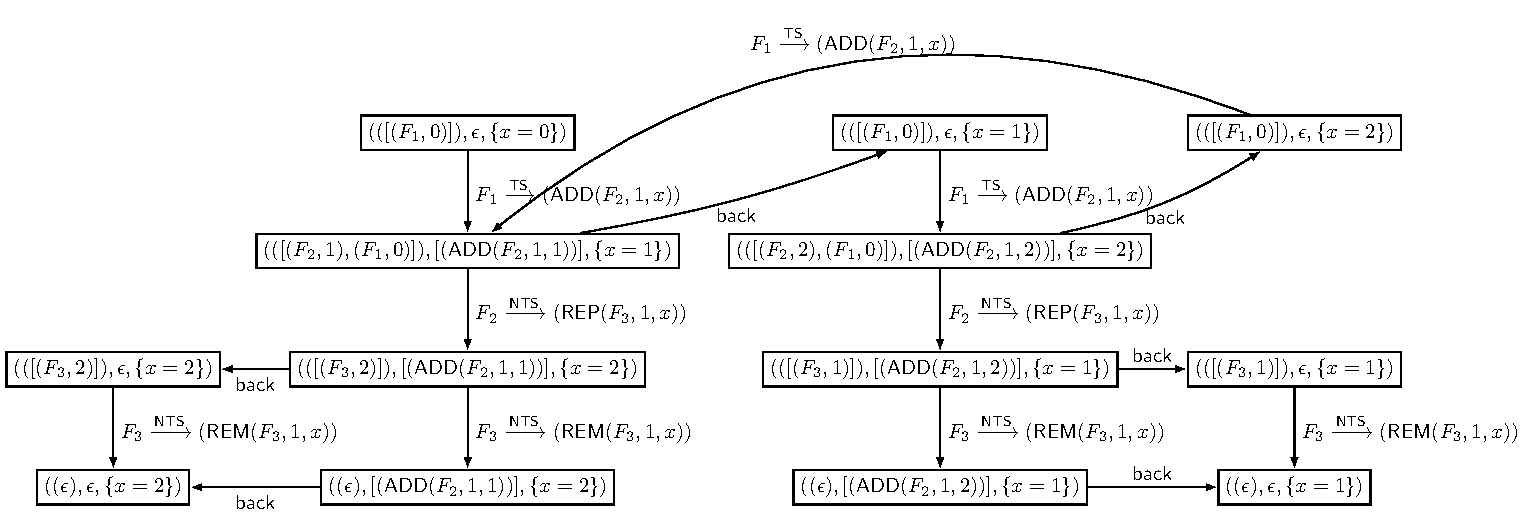
\includegraphics[scale = 0.6]{frg-example.pdf}
            \caption{Configurations that are reachable from the configuration $(([(F_1,0)]),\epsilon,\{x=0\})$ in $\Mm$}
                %in $\phi$
        % \vspace{-6mm}	
        \label{frg-example}
    \end{figure}


\end{example}



%!TEX root = main.tex

\subsection{Semantics of {$\AOAMASS$} for the other versions of Android}

As mentioned before, the semantics of {$\AOAMASS$} of different versions of Android are different. In the sequel, we illustrate the differences by focusing on $\IFAOAMASS$. The differences of the semantics of {$\AOAMASS$} can be found in the appendix. 

Before a formal description, let us first illustrate the differences using the following example. 
\begin{example}
    Let $\Mm = (\act,A,\frag,\lmd,\aft,\vgr, \Delta)$ be an {$\IFAOAMASS$}, where $\act = \{A,B,C,D\}$, for each $A' \in\act$, $\lmd(A') = \STD$, $\aft(A) = \aft(B) = 1$, and $\aft(C) = \aft(D) = 2$, moreover, $\Delta = \{\back\} \cup  \{\tau_i \mid 1\le i \le 6\} \cup \{\tau'_i \mid 1\le i \le 3\} $ such that 
        $\tau_1 = A\xrightarrow{\startactivity(\bot)}C$,
        $\tau_2 = C\xrightarrow{\startactivity(\ntkflag\wedge\mtkflag)}B$,
        $\tau_3 = B\xrightarrow{\startactivity(\ntkflag)}C$,
        $\tau_4 = C\xrightarrow{\startactivity(\bot)}D$,
        $\tau_5 = D\xrightarrow{\startactivity(\bot)}A$,
        $\tau_6 = A\xrightarrow{\startactivity(\ntkflag)}A$,
        $\tau'_1 = C\xrightarrow{\startactivity(\ntkflag\wedge\rtfflag)}D$,
        $\tau'_2 = C\xrightarrow{\startactivity(\rtfflag)}A$,
        $\tau'_3 = C\xrightarrow{\startactivity(\ntkflag)}B$.

We use the configuration $(([CA],A,\mainflag),([ADC],C,\ntkflag),([B],B,\ntkflag))$ to illustrate the difference. This configuration can be reached from the initial configuration $(([A],A,\mainflag))$ by the following sequence of transition rules: $\tau_1\ \tau_2\ \tau_3\ \tau_4\ \tau_5\ \tau_6\ \back$.
%    As shown in Figure~\ref{and-example}, the configuration $((([CA],A,\mainflag),([ADC],C,\ntkflag),([B],B,\ntkflag)),\neg\nohflag)$ is reached from the initial configuration $((([A],A,\mainflag)),\neg\nohflag)$ by the transition rules sequence $\tau_1',\tau_2',\tau_3',\tau_4',\tau_5',\tau_6',\back$.
The differences of semantics for different versions of Android are demonstrated by applying $\tau'_1, \tau'_2, \tau'_3$ on the configuration $(([CA],A,\mainflag),([ADC],C,\ntkflag),([B],B,\ntkflag))$ (see Figure~\ref{fig-diff-version}).     
\begin{itemize}
 \item If the transition $\tau'_1 = C\xrightarrow{\startactivity(\ntkflag \wedge \rtfflag)}D$ is applied, then for Android 11.0-13.0 the task $([ADC],C,\ntkflag)$ is moved to the top and the activity $D$ is reordered to the front, resulting in the configuration
        $$(([DAC],C,\ntkflag), ([CA],A,\mainflag), ([B],B,\ntkflag)),$$ 
        while for Android 6.0-10.0,  the activity $D$ is pushed after the task $([ADC],C,\ntkflag)$ is moved to the top, resulting in the configuration 
        $$(([DADC],C,\ntkflag), ([CA],A,\mainflag), ([B],B,\ntkflag)).$$
        This difference is explained by the fact that for Android 6.0-10.0, $\rtfflag$ is ignored when it is used together with $\ntkflag$.
        
%        there is a distinction in the generated configurations between Android 6.0-10.0 and Android 11.0-12.0. In Android 6.0-10.0, $D$ is directly added to the $C$-task instead of being placed on top of the $C$-task. This implies that in Android 6.0-10.0, $\rtfflag$ becomes irrelevant to the semantics when it is combined with $\ntkflag$.
        %
        \item If the transition $\tau'_2 = C\xrightarrow{\startactivity(\rtfflag)} A$ is applied,  then for all the versions of Android 6.0--13.0, except 7.0, $A$ is reordered to the front in the top task, resulting in the configuration 
        $$(([AC],A,\mainflag),([ADC],C,\ntkflag),([B],B,\ntkflag)).$$
        In Android 7.0, the top task is cleared and $A$ is pushed, resulting in the configuration
        $$(([A],A,\mainflag),([ADC],C,\ntkflag),([B],B,\ntkflag)).$$
        This difference is explained by the fact that for Android 7.0, when the top task is the main task where the started activity occurs but is not the top activity, $\rtfflag$ has the same effect as $\ctkflag$.
                %
        \item If the transition $\tau'_3 = C\xrightarrow{\startactivity(\ntkflag)} B$ is applied, then for all the versions of Android 7.0--12.0,  the $B$-task is moved to the top (without pushing a new instance of $B$), resulting in the configuration 
        $$(([B],B,\ntkflag), ([CA],A,\mainflag),([ADC],C,\ntkflag)).$$
        In Android 6.0, the $B$-task is not moved to the top, and an instance of $B$ is pushed to the top task directly, resulting in the configuration
        $$(([BCA],A,\mainflag),([ADC],C,\ntkflag), ([B],B,\ntkflag)).$$
       This difference is explained by the fact that the task allocation mechanism of Android 6.0 is different from the other versions, namely, in Android 6.0, only affinities are used for looking for a task, while for the other versions, real activities and affinities are used together to look for a task. 
       %        the generated configuration of Android 6.0 is different with other versions. In Android 6.0, $B$-task is not switched to the top. This implies that the task allocation mechanism of Android 6.0 has nothing to do with the real activities of tasks but only uses the affinities of tasks.
        % that is, $\rtfflag$ is irrelevant to the semantics in this case.
    \end{itemize}

\begin{figure}[htbp]
    % \vspace{-3mm}
\centering
        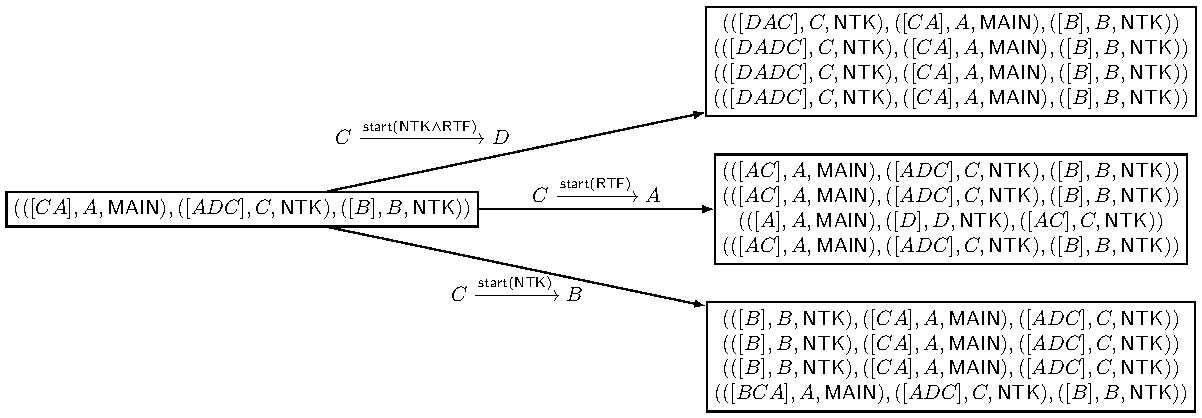
\includegraphics[scale = 0.7]{and-example.pdf}
\caption{Semantics of $\IFAOAMASS$ for different versions of Android, where the 1st, 2nd, 3rd, 4th line of the texts in the right boxes are configurations for Android 11.0--13.0, 8.0--10.0, 7.0, and 6.0 respectively}
    % \vspace{-6mm}	
    \label{fig-diff-version}
\end{figure}
\end{example}
%

In the sequel, we state the differences of the semantics of {$\IFAOAMASS$} models in details. To avoid tediousness, let us focus on the situation $\phi \models \neg \tohflag$. The differences for the situation $\phi \models \tohflag$ are similar. 

\subsubsection{Android 11.0, 12.0.}
The semantics of {\AMASS} for Android 11.0 and 12.0 are the same as Android 13.0. 

\subsubsection{Android 10.0, 9.0, and 8.0.}
The semantics for these three versions are the same and differ from that for Android 13.0 in the following sense: $\rtfflag$ is ignored when used together with $\ntkflag$. 
That is, for Android 10.0, 9.0, and 8.0, the semantics of $\IFAOAMASS$ for the case $\phi  \models \ntkflag \wedge \neg \ndmflag$ is adapted from Android 13.0 as follows.

\begin{itemize}
\item If $\phi \models \mtkflag$, then $\cdots$.
%
\item If $\phi \models \neg \mtkflag$, then
	\begin{itemize}
        \item if $\getrealtsk(\rho, B) = S_i$ or $\getrealtsk(\rho,B) = * \wedge\gettsk(\rho,B) = S_i$, then
		\begin{itemize}
			\item if $\phi \models \ctkflag$, then $\cdots$,
			\item if $\phi \models \neg \ctkflag$, then
			\begin{itemize}
				\item if $\phi \models \ctpflag$ and $B \in S_i$, then $\cdots$,
				\item if $\phi \models \ctpflag$ and $B \notin S_i$, then $\cdots$,
				\item if $\phi \models \neg \ctpflag$, then
				\begin{itemize}
						\item if $\getrealtsk(\rho, B) = S_i$ and $\zeta_i \neq \mainflag$, 
						then $\rho' = \mvtsktop(\rho, i)$,
						\item otherwise, 
						\begin{itemize}
							\item if $\phi \models \stpflag$ and $\topact(S_i) = B$, or $\phi \models \stpflag \wedge \pitflag$ and $i = 1$ and $\preact(S_1) = B$, then $\rho' = \mvtsktop(\rho, i)$,
							\item otherwise, $\rho'=\push(\mvtsktop(\rho, i), B)$,
						\end{itemize}
				\end{itemize}
			\end{itemize}
		\end{itemize}
	    %
	\item if $\gettsk(\rho, B) = *$, then $\cdots$.
	\end{itemize}
\end{itemize}
%When $\phi \models \ntkflag \wedge \neg\ndmflag\wedge\neg \mtkflag$, $\rtfflag$ is ignored. 
%
\hide{
\begin{itemize}
\item If $\phi \models \mtkflag$, then $\cdots$. 
\item If $\phi \models \neg \mtkflag$, then 
\begin{itemize}
    \item if $\getrealtsk(\rho, B) = S_i$ or $\getrealtsk(\rho,B) = * \wedge\gettsk(\rho,B) = S_i$, then
    \begin{itemize}
    \item if $i \neq 1$, then 
        \begin{itemize}
            \item if $\phi \models \ctkflag$, then $\cdots$ 
            \item if $\phi \models \neg \ctkflag$, then $\cdots$
                \begin{itemize}
                    \item if $\phi \models\ctpflag$ and $B \in S_i$, then $\cdots$
                    \item if $\phi \models\ctpflag$ and $B \notin S_i$, then $\cdots$
                    \item if $\phi \models\neg\ctpflag$, then
                    \begin{itemize}
                            \item if $\getrealtsk(\rho,B) = S_i$ and $\zeta_i \neq \mainflag$, then $b' = \neg \nohflag$, moreover,
                            \begin{itemize}
                                \item if $b = \neg \nohflag$, then $\rho'=\mvtsktop(\rho, i)$,
                                \item otherwise, $\rho' = \rmact(\mvtsktop(\rho, i), 2, 1)$, 
                            \end{itemize}
                            \item otherwise ($\getrealtsk(\rho,B) = S_i$ and $\zeta_i = \mainflag$ or $\getrealtsk(\rho,B) = * \wedge\gettsk(\rho,B) = S_i$), 
                            \begin{itemize}
                                \item if $\phi\models\stpflag$ and $\topact(S_i) = B$, then $b' = \neg \nohflag$, moreover,
                                \begin{itemize}
                                    \item if $b = \neg \nohflag$, then $\rho'=\mvtsktop(\rho, i)$,
                                    \item otherwise, $\rho' = \rmact(\mvtsktop(\rho, i), 2, 1)$, 
                                \end{itemize}
                                \item otherwise, $b' = \nohflag$ iff $\phi \models \nohflag$, moreover, 
                                \begin{itemize}
                                    \item if $b = \neg \nohflag$, then $\rho'=\push(\mvtsktop(\rho, i), B)$,
                                    \item otherwise, $\rho' = \rmact(\push(\mvtsktop(\rho, i), B), 2, 1)$, 
                                \end{itemize}
                        \end{itemize}
                    \end{itemize}
                \end{itemize}
        \end{itemize}
    \item otherwise ($i  = 1$),  
    \begin{itemize}
        \item if $\phi \models \ctkflag$, then $\cdots$, 
        \item if $\phi \models \neg \ctkflag$, then 
        \begin{itemize}
            \item if $\phi \models \ctpflag$ and $B \in S_1$, then $\cdots$
%				\begin{itemize}
%					\item if $\phi\models \neg \stpflag$, then $b' = \nohflag$ iff $\phi \models \nohflag$, 
%					\item otherwise, $b' = \neg \nohflag$,
%				\end{itemize}
            \item if $\phi \models \ctpflag$ and $B\notin S_1$, then $\cdots$
            \item if $\phi \models \neg \ctpflag$, then
            \begin{itemize}
                \item if $\getrealtsk(\rho,B) = S_1$ and $\zeta_1 \neq \mainflag$, then $\rho' = \rho$ and $b' = b$,
                \item otherwise ($\getrealtsk(\rho,B) = S_1$ and $\zeta_i = \mainflag$ or $\getrealtsk(\rho,B) = * \wedge\gettsk(\rho,B) = S_1$), 
                \begin{itemize}
                    \item if $\phi\models\stpflag$ and $A = B$, or $\phi \models\stpflag\wedge\pitflag$ and $\preact(\rho) = B$, then $\rho' = \rho$ and $b' = b$, 
                    \item otherwise, $b' = \nohflag$ iff $\phi \models \nohflag$, moreover, 
                    \begin{itemize}
                        \item if $b = \neg \nohflag$, then $\rho'=\push(\rho, B)$,
                        \item otherwise, $\rho' = \rmact(\push(\rho, B), 1, 2)$, 
                    \end{itemize}
                \end{itemize}
            \end{itemize}
        \end{itemize}
    \end{itemize}
\end{itemize}
\item if $\gettsk(\rho, B) = *$, then $\cdots$. 
\end{itemize}
\end{itemize}
}
Note that the parts of the semantics denoted by $\cdots$ are the same as Android 13.0, and in the semantics for the situation $\phi \models \neg \ctpflag$, the flag $\rtfflag$ has no effects, thus is ignored.  


%Moreover, the semantics in the case $\phi \models \tohflag$ should be similarly adapted for $\rtfflag$.

%$\rtfflag$ flag will be omitted when $\phi\models\ntkflag$ or $\lmd(A) = \singleinstance$ for $A\xrightarrow{\alpha(\phi)}B$. More precisely, the semantics can be adapted from that for Android 12.0 as follows:
%\begin{itemize}
%    \item for the subcase $\phi \models \ntkflag\wedge \neg \mtkflag$, or $\lmd(A) = \singleinstance$ and $\phi  \models \neg \mtkflag$ of the case $\lmd(B) = \standard$ and $\lmd(B) = \singletop$, 
 %       remove $\rtfflag$ in the formulae $\phi$, and remove the item which constraint is $\phi\models\rtfflag\wedge\neg\ctpflag\wedge\neg\ctkflag$ and $B\in S_j$.
%\end{itemize}

\subsubsection{Android 7.0.}
The semantics for Android 7.0 is close to that of Android 10.0 (or 9.0, 8.0) but differs from it in the following two aspects:  1) the effect of $\ndmflag$ is the same as that of $\ntkflag$, 2)
when $\phi \models \neg \ntkflag \wedge \neg\ndmflag \wedge \neg\ctpflag$, if the top task is the main task where the started activity occurs but is not the top activity, then $\rtfflag$ has the same effect as $\ctkflag$. More precisely, for Android 7.0, only two cases $\phi \models \ntkflag$ and $\phi  \models \neg \ntkflag$ are considered, where the semantics for the case $\phi \models \ntkflag$ inherits that of $\phi \models \ntkflag \wedge \neg \ndmflag$ for Android 10.0, while the semantics for the case $\phi  \models \neg \ntkflag$ is adapted from that of $\phi \models \neg \ntkflag \wedge \neg \ndmflag$ for Android 10.0 as follows. 
%
%
%        \item if $\phi \models \rtfflag \wedge \neg \ctpflag$ and $B \in \toptsk(\rho)$, then
 %        $\rho'=\mvacttop(\rho, B)$,
%
\begin{itemize}
	\item If $\phi \models \ctpflag$ and $B \in \toptsk(\rho)$, then $\cdots$.
	\item If $\phi \models \ctpflag$ and $B \not \in \toptsk(\rho)$, then $\cdots$.
	\item If $\phi \models \neg \ctpflag$, then
		\begin{itemize}
    			\item if $\phi \models \rtfflag$ and $B \in \toptsk(\rho)$, then
    			\begin{itemize}
                    \item if $\zeta_i = \mainflag$, then $\rho' = \clrtsk(\rho, B)$,
                    \item otherwise, $\rho' = \mvacttop(\rho, B)$,
                    % \begin{itemize}
                    %         \item if $b = \neg \nohflag$, then $\rho'= \mvacttop(\rho, B)$, 
                    %         \item otherwise, $\rho' = \rmact(\mvacttop(\rho, B), 1, 2)$, 
                    % \end{itemize}
    			\end{itemize}
			\item if $\phi \models \rtfflag$ and $B \not \in \toptsk(\rho)$, then $\cdots$,
			\item if $\phi \models \neg \rtfflag$, then $\cdots$.
		\end{itemize}
\end{itemize}
%Intuitively, when $\phi \models \rtfflag \wedge \neg \ctpflag$, $B \in \toptsk(\rho)$, and additionally the top task is the main task, the top task is cleared before pushing $B$.

%$\ndmflag$ has the same effects with $\ntkflag$, and for each item $\ndmflag$ and $\neg\ndmflag$ are removed.

%In Android 7.0, $\rtfflag$ flag will clear the task when the current task is the main task. More precisely, the semantics of Android 7.0 is defined as follows.
%\begin{itemize}
%    \item for the subcase $\lmd(A) \neq \singleinstance$ and $\phi \models \neg \ntkflag$ of the case $\lmd(B) = \standard$ and $\lmd(B) = \singletop$, replace the constraint with $\phi\models\rtfflag\wedge\neg\ctpflag$ and $B\in S_j$ and $b_1=0$,
%        of the item which constraint is $\phi\models\rtfflag\wedge\neg\ctpflag$ and $B\in S_j$,
%        and add an item: if $\phi\models\rtfflag\wedge\neg\ctpflag$ and $B\in S_j$ and $b_1=1$,
%        then $\rho' = \push(\clrtsk(\rho),B)$.
%\end{itemize}

\subsubsection{Android 6.0.}
The semantics for Android 6.0 differs from that of Android 10.0 (or 9.0, 8.0) in the following two aspects: 1) the effect of $\ndmflag$ is the same as that of $\ntkflag$, 2) the task allocation mechanism of Android 6.0 does not use the real activities of tasks and only relies on affinities. 
%
More precisely, for Android 6.0, only two cases $\phi \models \ntkflag$ and $\phi  \models \neg \ntkflag$ are considered, where
the semantics for the case $\phi  \models \neg \ntkflag$ inherits that of $\phi \models \neg \ntkflag \wedge \neg \ndmflag$, 
and the semantics for the case $\phi \models \ntkflag$ is adapted from that of $\phi \models \ntkflag \wedge \neg \ndmflag$ for Android 10.0 as follows, where the conditions involving $\getrealtsk(\rho, B)$ and $\gettsk(\rho, B)$ are simplified into the conditions involving only $\gettsk(\rho, B)$, moreover, we do not need to distinguish whether a task is the main task or not.  
\begin{itemize}
\item If $\phi \models \mtkflag$, then $\cdots$.
%
\item If $\phi \models \neg \mtkflag$, then
	\begin{itemize}
        \item if $\gettsk(\rho,B) = S_i$, then
		\begin{itemize}
			\item if $\phi \models \ctkflag$, then $\cdots$,
			\item if $\phi \models \neg \ctkflag$, then
			\begin{itemize}
				\item if $\phi \models \ctpflag$ and $B \in S_i$, then $\cdots$,
				\item if $\phi \models \ctpflag$ and $B \notin S_i$, then $\cdots$,
				\item if $\phi \models \neg \ctpflag$, then
				\begin{itemize}
                    \item if $\phi \models \stpflag$ and $\topact(S_i) = B$, or $\phi \models \stpflag \wedge \pitflag$ and $i = 1$ and $\preact(S_1) = B$, then $\rho' = \mvtsktop(\rho, i)$,
                    \item otherwise, $\rho'=\push(\mvtsktop(\rho, i), B)$,
				\end{itemize}
			\end{itemize}
		\end{itemize}
	    %
	\item if $\gettsk(\rho, B) = *$, then $\cdots$.
	\end{itemize}
\end{itemize}
\hide{
\begin{itemize}
\item If $\phi \models \mtkflag$, then $\cdots$.
\item If $\phi \models \neg \mtkflag$, then 
\begin{itemize}
    \item if $\gettsk(\rho,B) = S_i$, then
%    // {\it $\getrealtsk(\rho, B) = S_i$ or $\getrealtsk(\rho,B) = * \wedge\gettsk(\rho,B) = S_i$ is replaced by $\gettsk(\rho,B) = S_i$}
    \begin{itemize}
    \item if $i \neq 1$, then 
        \begin{itemize}
            \item if $\phi \models \ctkflag$, then $\cdots$ 
            \item if $\phi \models \neg \ctkflag$, then $\cdots$
                \begin{itemize}
                    \item if $\phi \models\ctpflag$ and $B \in S_i$, then $\cdots$
                    \item if $\phi \models\ctpflag$ and $B \notin S_i$, then $\cdots$
                    \item if $\phi \models\neg\ctpflag$, then
%                    \begin{itemize}
%                            \item if $\getrealtsk(\rho,B) = S_i$ and $\zeta_i \neq \mainflag$, then $b' = \neg \nohflag$, moreover,
%                            \begin{itemize}
%                                \item if $b = \neg \nohflag$, then $\rho'=\mvtsktop(\rho, i)$,
%                                \item otherwise, $\rho' = \rmact(\mvtsktop(\rho, i), 2, 1)$, 
%                            \end{itemize}
%                            \item otherwise ($\getrealtsk(\rho,B) = S_i$ and $\zeta_i = \mainflag$ or $\getrealtsk(\rho,B) = * \wedge\gettsk(\rho,B) = S_i$), 
                            \begin{itemize}
                                \item if $\phi\models\stpflag$ and $\topact(S_i) = B$, then $b' = \neg \nohflag$, moreover,
                                \begin{itemize}
                                    \item if $b = \neg \nohflag$, then $\rho'=\mvtsktop(\rho, i)$,
                                    \item otherwise, $\rho' = \rmact(\mvtsktop(\rho, i), 2, 1)$, 
                                \end{itemize}
                                \item otherwise, $b' = \nohflag$ iff $\phi \models \nohflag$, moreover, 
                                \begin{itemize}
                                    \item if $b = \neg \nohflag$, then $\rho'=\push(\mvtsktop(\rho, i), B)$,
                                    \item otherwise, $\rho' = \rmact(\push(\mvtsktop(\rho, i), B), 2, 1)$, 
                                \end{itemize}
                           \end{itemize}
%                    \end{itemize}
                \end{itemize}
        \end{itemize}
    \item otherwise ($i  = 1$),  
    \begin{itemize}
        \item if $\phi \models \ctkflag$, then $\cdots$, 
        \item if $\phi \models \neg \ctkflag$, then 
        \begin{itemize}
            \item if $\phi \models \ctpflag$ and $B \in S_1$, then $\cdots$
%				\begin{itemize}
%					\item if $\phi\models \neg \stpflag$, then $b' = \nohflag$ iff $\phi \models \nohflag$, 
%					\item otherwise, $b' = \neg \nohflag$,
%				\end{itemize}
            \item if $\phi \models \ctpflag$ and $B\notin S_1$, then $\cdots$
            \item if $\phi \models \neg \ctpflag$, then
%            \begin{itemize}
%                \item if $\getrealtsk(\rho,B) = S_1$ and $\zeta_1 \neq \mainflag$, then $\rho' = \rho$ and $b' = b$,
%                \item otherwise ($\getrealtsk(\rho,B) = S_1$ and $\zeta_i = \mainflag$ or $\getrealtsk(\rho,B) = * \wedge\gettsk(\rho,B) = S_1$), 
                \begin{itemize}
                    \item if $\phi\models\stpflag$ and $A = B$, or $\phi \models\stpflag\wedge\pitflag$ and $\preact(\rho) = B$, then $\rho' = \rho$ and $b' = b$, 
                    \item otherwise, $b' = \nohflag$ iff $\phi \models \nohflag$, moreover, 
                    \begin{itemize}
                        \item if $b = \neg \nohflag$, then $\rho'=\push(\rho, B)$,
                        \item otherwise, $\rho' = \rmact(\push(\rho, B), 1, 2)$, 
                    \end{itemize}
%                \end{itemize}
            \end{itemize}
        \end{itemize}
    \end{itemize}
\end{itemize}
\item if $\gettsk(\rho, B) = *$, then $\cdots$. 
\end{itemize}
\end{itemize}
}
%remove the item and sub-items for the constraint $\getrealtsk(\rho, B) = S_i$ and $\zeta_i \neq \mainflag$, and replace  the following constraint with  $ \gettsk(\rho, B) = S_i$: $\getrealtsk(\rho, B) = S_i$ and $\zeta_i = \mainflag$, or $\getrealtsk(\rho, B) = * \wedge \gettsk(\rho, B) = S_i$.
	%
%	remove the item corresponding to the constraint $\getrealtsk(\rho, B) = S_j$, moreover, replace the constraint $\getrealtsk(\rho, B) = *$ and $\gettsk(\rho, B) = S_j$ with $\gettsk(\rho, B) = S_j$.
	%
%
We remark that the unexpected behavior of $\rtfflag$ for Android 7.0, that is, $\rtfflag$ behaves the same as $\ctkflag$ in some cases, does not occur in Android 6.0. 



\smallskip

We have defined the semantics of {$\AMASS$} in this section. To go one step further, we would like to validate the semantics against the actual behaviors of Android apps w.r.t. the multitasking mechanism between activities and fragments. Moreover, we would like to do some static analysis of the behaviors of Android apps related to the multitasking mechanism between activities and fragments. To facilitate these two tasks, in the next two sections, we build {\AMASS} models out of APK files of Android apps and encode the reachability problem of {\AMASS} models into the model checking problem in the input format of nuXmv model checker \cite{nuXmv}. 





\section{Generating {\AMASS} models from APK files}\label{sec:apk2amass}
%!TEX root = main.tex

%\subsection{Extraction of the {\AMASS} models out of APK files}

The goal of this section is to show how we build {\AMASS} models out of the APK files of the Android apps.

%To analyze the behaviors of Android apps with respect to the multitasking mechanism, it is necessary to extract the {\AMASS} model out of the APK file of Android apps.

%\subsection*{Static Extraction}
In Android apps, switching between components is by sending inter-component communication (ICC) messages to the Android system. 
Each ICC message is represented by an \texttt{Intent} object that carries a set of data items.
By resolving 
the ICC messages, we can extract both the source and destination of %a transition 
the switching and the data items it carries.  
%Thus, to construct an {\AMASS} model for an Android app, the precise resolution of ICC messages makes the first step.
%\tl{what does it mean ICC resolution?}


The recent work \cite{YZ+22} studied the available ICC resolution tools and performed a practical evaluation on both hand-crafted benchmarks as well as large-scale real-world apps.
The evaluation shows that (1) the fragment is a key feature that is widely used in the component transitions; (2) most of state-of-the-art ICC resolution tools miss the ICCs involving activities and fragments. 
A recent %ICC resolution 
tool \textit{ICCBot}~\cite{ICCBot_paper} %is a recently-developed , which 
resolves the component transitions connected by fragments and activities,  %. Compared with the state-of-the-art tools, ICCBot 
achieves a higher success rate and accuracy.
% 
%Although we can use ICCBot to obtain a component transition graph from an APK file, there 
However, ICCBot is insufficient for obtaining an {\AMASS} model for the following two reasons. %. More specifically,
\begin{itemize}
\item ICCBot fails to decompile the APK files of some commercial apps, thus their models cannot be constructed. 
%
\item {\AMASS} models contain more information about the component transitions, in particular, ICCBot ignores the API ``addToBackStack()'' which can allow pushing transactions to the fragment transaction stack, and ignores the API \texttt{finish()} which can pop the current activity.
% the fragment transactions when manipulating fragments,
%
\end{itemize}

To this end, we extend ICCBot to ICCBot$_{\AMASS}$ in the following aspects. % to extract the {\AMASS} models.
%Specifically,  ICCBot$_{AMASS}$ extends  ICCBot in the following aspects. 
\begin{itemize}
\item At first, ICCBot$_{\AMASS}$ %extends ICCBot to 
records the calls to the API \texttt{finish()} and associates them with the corresponding calls to \texttt{startActivity()} or \texttt{startActivityForResult()}. This enables ICCBot$_{\AMASS}$ to accurately track the termination of the activities and identify transition rules that are affected by these terminations. 
%
\item Additionally, ICCBot$_{\AMASS}$ monitors the calls of the API \texttt{addToBackstack()}, so that the transition rules involving fragments can be accurately constructed. In contrast, ICCBot does not record \texttt{addToBackstack()}. Therefore, it misses the information $\mu \in \{\opstack, \nopstack\}$ in the transition rules $A \xrightarrow{\mu} T$ or $F \xrightarrow{\mu} T$.
%
\item Moreover, ICCBot$_{\AMASS}$ provides means to take cross-app ICCs into consideration when constructing {\AMASS} models.
%
\item Finally, for the commercial apps that cannot be decompiled,  ICCBot$_{\AMASS}$ applies a dynamic approach to extract the {\AMASS} models. 
\end{itemize}
% records the calls to the API \texttt{finish()} and attach them to the occurrences of \texttt{startActivity()} or \texttt{startActivityForResult()}.
% extracts the intent flags for starting activities.  
%ICCBot ignored the intent flags $\phi$, it is extended to 
% ICCBot$_{\AMASS}$ tracks the usage of the API \texttt{addFlags()} on each Intent object and extract its integer value. Because this integer value is obtained by combining the intent flags with bit operations, we need to reverse the bit operations to obtain the original intent flags.
%
%\item 
% Moreover, ICCBot$_{\AMASS}$ %extends ICCBot to 
% records the calls to the API \texttt{finish()} and attach them to the occurrences of \texttt{startActivity()} or \texttt{startActivityForResult()}.
%
%\item 
%
%Furthermore, ICCBot$_{AMASS}$ 
% It also tracks the occurrences of the API \texttt{addToBackstack()} to record the fragment transactions.


%for the cross-app ICC, ICCBot$_{\AMASS}$ provides users with the option to apply the necessary APK files related to the cross-app ICC, assisting ICCBot$_{\AMASS}$ in constructing the comprehensive {\AMASS} model. More specifically, ICCBot$_{\AMASS}$ constructs an {\AMASS} model that includes the activities, fragments, transition rules, and other components of the relevant apps and the main activity of the analyzed app is set as the main activity $A_0$ of the {\AMASS} model. In the sequel, these apps can be treated as one app for further analysis. Out of the extracted models from F-Droid (3,471 models) and Google Play (4,612 models), a total of 311 (F-Droid) and 501 (Google Play) models involve cross-app ICC. To identify these relevant apps, we search for their package names mentioned in the cross-app ICC. Consequently, we discover 125 (F-Droid) and 221 (Google Play) related APK files that facilitate the construction of the {\AMASS} models.

In the sequel, we describe more details about how ICCBot$_{\AMASS}$ takes cross-app ICCs into consideration as well as utilizes a dynamic approach to construct {\AMASS} models for these apps that cannot be decompiled.

\paragraph{Model extraction for cross-app ICCs.} 
If for an app, the multiple APK files that are involved in the cross-app ICCs of this app are provided, then ICCBot$_{\AMASS}$ can construct an {\AMASS} model that captures the behaviors of all these multiple APK files. The algorithm goes as follows. 
\begin{enumerate}
\item At first, for the APK file corresponding to an app, ICCBot$_{\AMASS}$ constructs an {\AMASS} model, where the cross-app ICCs starting from this app are recorded but not processed. 
%
\item Then for the model, we try to manually identify the APK files involved in these cross-app ICCs by searching for their package names. 
%
\item If the APK files involved in the cross-app ICCs are identified successfully for the app, then all these multiple APK files, including the original APK file for the app, are processed and an {\AMASS} model to capture the behaviors of all these apps is constructed. 
\end{enumerate}
Afterwards, these models can be analyzed just as a model extracted from an app containing no cross-app ICCs. 

%Out of the models that extracted from the APK files, 
%Out of the 3,471 models that are extracted from the APK files in F-Droid (called F-Droid models for short) and 4,612 models that are extracted from the APK files in Google Play (called Google-Play models for short), ICCBot$_{\AMASS}$ discovers that 311 F-Droid models and 501 Google-Play models respectively involve cross-app ICCs. 
%Note that although these models are discovered to involve cross-app ICCs, each of these models is extracted from \emph{one} APK file and the cross-app ICCs therein have not been dealt with yet. 
%To remedy this, we tried to manually identify the APK files involved in these cross-app ICCs by searching for their package names. In the end, for 125 F-Droid apps and 211 Google-Play apps respectively, we provided the missing APK files involved in the cross-app ICCs of these apps and successfully constructed the {\AMASS} models for them where the cross-app ICCs are modeled. Afterwards, these models can be analyzed in the same way as a model that is extracted from one APK file. 

\paragraph{Dynamic model extraction for unsuccessfully decompiled APK files. }
Roughly speaking, the algorithm to extract {\AMASS} models dynamically from APK files works as follows.
\begin{enumerate}
\item We first execute all click events of the foreground activity to search for new activities. 
%
\item When clicking some events in the foreground activity, some new UI widgets, e.g. menu widgets, may appear (though the foreground activity is unchanged), resulting in some new click events.  When executing these newly produced click events, some UI widgets may appear and even more new click events can be produced. The click events in the foreground activity are organized hierarchically.  
%	
\item We apply a depth-first search to execute all the sequences of hierarchically-organized click events, up to some depth. If a new activity is found,  the associated transition rule for starting the new activity is produced, where the intent flags are guessed. For instance, if a non-top task is moved to the top and a new instance of the activity $B$ of the ``standard'' launch mode is pushed to it, then the ``$\ntkflag$'' flag can be guessed. 
\end{enumerate}

%Android Debug Bridge (adb) is a versatile command-line tool that lets you communicate with a device.
%Given an Android app, starting from the main activity of the app, intuitively, we %the following procedure is executed to 
%extract the {\AMASS} model dynamically as follows.
%We first execute all click events of the foreground activity to search for new activities as well as the transitions to start the new activities. 
	
 

%\begin{tcolorbox}[width=1.0\linewidth, title={Procedure of UIAutomator to extract {\AMASS} model}]
% Execute all click events of the foreground activity to search for new activities as well as the transitions to start the new activities. 
% 
% When clicking some events in the foreground activity, some new UI widgets, e.g. menu widgets, may appear (though the foreground activity is unchanged), resulting in some new click events. 
% 
% When executing these newly produced click events, some UI widgets may appear and even more new click events can be produced. Thus, the click events in the foreground activity are organized hierarchically.  
% 
% We apply a depth-first search to execute all the sequences of hierarchically-organized click events, up to some depth. If a new activity is found, then the associated transition for starting the new activity is produced, where the intent flags are guessed. For instance, if a new instance of the activity $B$ of the ``standard'' launch mode is pushed to a non-top task, then the ``$\ntkflag$'' flag can be guessed. 
%\end{tcolorbox}
 
%Note that the launch modes and the task affinities of activities can be obtained from the manifest files.  
 

% these new click events, that is, we use UIAutomator to execute one click event, then execute one of the newly produced  click events, before  
%
%\end{enumerate}

%\end{itemize}
%$A \xrightarrow{\mu} T$ or $F \xrightarrow{\mu} T$, $A$ or $F$ is the caller activity or fragment, $T$ is the fragment transaction

%As ICCBot considers more about the transition among components but not the construction of an {\AMASS} model, we extend the original ICCBot to ICCBot$_{AMASS}$ with more complete Intent and Fragment modeling.

%Recall that the transition $A \xrightarrow{\alpha(\phi)} B$ contains a caller activity $A$, a callee activity $B$, an action $\alpha$, and intent flags $\phi$. 
%In terms of modeling by an {\AMASS}, the action is \textit{start} when \texttt{startActivity()} or \texttt{startActivityForResult()} is invoked, while it is \textit{finishStart} when \texttt{finish()} is invoked.
%And for the transition $A \xrightarrow{\mu} T$ or $F \xrightarrow{\mu} T$, $A$ or $F$ is the caller activity or fragment, $T$ is the fragment transaction. 
%For the {\AMASS} modeling, the fragment transaction comprises \textit{add}, \textit{replace} and \textit{addBack} when the corresponding APIs \texttt{add()}, \texttt{replace()}, and \texttt{addToBackstack()} are invoked.

%In the original ICCBot, the intent flags $\phi$ were not modeled. So we track the usage of API \texttt{addFlags()} on each Intent object and extract its integer value. Considering that the integer value is obtained by combining the intent flags with bit operations, we reverse the bit operations to obtain the original intent flags.
%Besides, the original ICCBot ignores the status of a component after starting, which means that only the operations like start, add and replace are considered. 
%To construct an {\AMASS} model, we extend it by capturing other actions, like finish and addToBackstack and recording their behaviors.
%Finally, based on the component graph provided by ICCBot, we generate AMASS that contains the activity transition $A \xrightarrow{\alpha(\phi)} B$ and fragment loading transition $E \xrightarrow{\beta} F$ and excludes other irrelevant edges.
%After extending to ICCBot$_{AMASS}$, we get the transitions among activities and fragments, as well as the actions that are performed along with a transition.
%Adopting this information, we could construct the AMASS for each app.  
%
%%%%%%%%%%%%%%%%%%%removed%%%%%%%%%%%%%%%%%%%%%%%%
%%%%%%%%%%%%%%%%%%%removed%%%%%%%%%%%%%%%%%%%%%%%%
% \hide{
% Nevertheless, the aforementioned procedure does not work very well while dealing with some commercial apps which could not be decompiled. 
% To tackle this, we propose a dynamic method to extract the transition rules set of the AMASS model from APK file, our algorithm is based on the following two step procedure.
% \begin{enumerate}
%     \item We use UIAutomator to search the new activities by executing the clickable events in the foreground activity, and guess the transition rule via the evolution of the configuration then update the transition rules set.
%     \item For each new activity, we repeat the step 1 until there is no new activity found.
% \end{enumerate}

\begin{algorithm}[htbp]
  \SetAlgoLined
  \tcc*[h]{Two global variables: $\Delta$ and $acts$}\;
  $\rho$ $\leftarrow$ $adb.getTasks()$\;
  $topAct$ $\leftarrow$ $adb.getTopActivity()$\;
  $visitedActs$ $\leftarrow$ $\{topAct\}$\;
  $DynDFS(\rho,topAct,[],d)$\;

  \While{$acts \neq \emptyset$} {
      \ForEach{$(newAct, newEvents) \in acts$}{ 
     \eIf{$newAct \in visitedActs$}{
         $acts \leftarrow acts-\{(newAct, newEvents)\}$\;
             continue\;
         }{
          $visitedActs$ $\leftarrow$ $visitedActs \cup \{newAct\}$\;
          $UIAutomator.restart()$\;
          \ForEach{$event \in newEvents$}{ 
              $UIAutomator.click(event)$\;
          }
          $\rho$ $\leftarrow$ $ADB.getTasks()$\;
          $DynDFS(\rho,newAct,newEvents,d)$\;
      }
  }
  }
    \caption{$AMASSExplore()$}
    \label{alg-explpore}
\end{algorithm}



The pseudo-code of the dynamic model-extraction algorithm is given in Algorithm~\ref{alg-explpore}, namely, the procedure $AMASSExplore()$.  
The procedure utilizes two global variables, $\Delta$ and $acts$, where $\Delta$ represents the current set of transition rules that are discovered so far, and $acts$ stores the pairs $(A, events)$, where $A$ is an activity and $events$ is a sequence of click events so that from the main activity, if these click events are executed by UIAutomator, then an instance of $A$ is started. The procedure $AMASSExplore()$ calls the procedure $DynDFS(\rho, srcAct, events, d)$ (see Algorithm~\ref{alg-dyndfs}) to do a depth-first search for new activities, starting from $srcAct$, up to the depth $d$ (i.e. the length of the click events reaching a new activity). The two procedures relies on some APIs of UIAutomator and ADB, whose meanings are described below.  
\begin{itemize}
\item $UIAutomator.getClickEvents()$ returns the set of clickable events in the foreground activity of the app under test,
\item $UIAutomator.click(e)$ executes the click-event $e$,
\item $UIAutomator.restart()$ restarts the the app under test,
\item $ADB.getTasks()$ returns the content of the back stack. 
\end{itemize}


For each $(newAct, newEvents) \in acts$, $AMASSExplore()$ calls the procedure $DynDFS(\rho, newAct, newEvents, d)$ to search dynamically for new activities, starting from $newAct$, and store the newly discovered activities as well as the corresponding sequences of click events into $acts$, up to the depth $d$. Here $d$ represents the length of the click-events sequence required to reach the new activity from $newAct$. Note that $newEvents$ are used by UIAutomator to reach $newAct$ starting from the main activity.  In some cases, pressing buttons may not start a new activity, but instead, new widgets appear (e.g., the menu widget), requiring us to continue searching for new click-events in these widgets to reach the new activity.

\begin{algorithm}[htbp]
  \SetAlgoLined
  \SetKwInOut{Input}{input}
    \SetKwInOut{Output}{output}
  \Input{$\rho, srcAct, events, d$}
\tcc*[h]{Dynamic depth-first search new activity with UIAutomator, up to depth $d$}\;
         \uIf{$d > 0$}{
                 \ForEach{$event \in UIAutomator.getClickEvents()$}{ 
                     $UIAutomator.click(event)$\;
                     $newAct$ $\leftarrow$ $ADB.getTopActivity()$\;
                     $newEvents$ $\leftarrow$ $events\cdot event$\;
        \uIf{$newAct = srcAct$}{
            \uIf{$d>1$}{
                $DynDFS(\rho, srcAct, newEvents, d - 1)$\;
                 \tcc*[h]{Decrement $d$ and continue the dynamic DFS.}\;
            }
            \Else {
                 $UIAutomator.restart()$\;
                 \ForEach{$event \in events$}{ 
                     $UIAutomator.click(event)$\;
                 }
            }
         }         
         \Else {
             \tcc*[h]{Discover new transitions and refine the AMASS model}\;             
             $\rho'$ $\leftarrow$ $ADB.getTasks()$\;
             $\tau'$ $\leftarrow$ $guessTrans$($srcAct$, $\rho$, $newAct$, $\rho'$)\;
             $\Delta$ $\leftarrow$ $\Delta\cup \{\tau'\}$\;
             $acts$ $\leftarrow$ $acts\cup \{(newAct,newEvents)\}$\;
             $UIAutomator.restart()$\;
             \ForEach{$event \in events$}{ 
                 $UIAutomator.click(event)$\;
             }
         }
    }
} 
    \caption{$DynDFS(\rho, srcAct, events, d)$}
    \label{alg-dyndfs}
\end{algorithm}


If a new activity is found during the execution of the procedure $DynDFS(\rho, srcAct, Events, d)$, with $\rho'$ being the current configuration, then the function $guessTrans(srcAct, \rho, newAct, \rho')$ is used to infer the intent flags based on the evolution of the configuration, so that a new transition rule $\tau'$ can be formed and put into $\Delta$. Moreover, the sequence of click events that reach $newAct$ from $srcAct$ is recorded in $newEvents$ and the pair $(newAct, newEvents)$ is put into $acts$.  
In order to continue searching for new activities, we need to return to the activity $srcAct$. Instead of pressing the back button, we restart the app and execute the corresponding $events$ using UIAutomator. This is necessary because in some cases, pressing the back button may not allow us to reach the previous activity, as indicated by the semantics in Section~\ref{sec:amass}.


%UIAutomator to discover new activities within the activities stored in $acts$, until no new activity is found. Each time $DynDFS()$ is called to search for activity $A$ with $(A, events) \in acts$, we need to reach $A$ by restarting the app and executing the corresponding $events$ using UIAutomator. The depth here represents the length of the click-events sequence required to reach the new activity from the foreground activity. In some cases, pressing buttons may not change the foreground activity, but instead, new widgets appear (e.g., the menu widget), requiring us to continue searching for new click-events in these widgets to reach the new activity.


% The aforementioned algorithm is presented as the procedure $AMASSExplore()$ in Algorithm~\ref{alg-explpore}, which uses tow global variables $\Delta$ and $acts$, where $\Delta$ is the current transition rules set of the AMASS model (since it may be dynamically modified in the Algorithm~\ref{alg-dyndfs}), $acts$ stores the set of the pair in form $(A,events)$ where $events$ is the click-events sequence which could be executed by UIAutomator from the main activity of the app to reach the activity $A$. Specifically,
% \begin{itemize}
%     \item the procedure $AMASSExplore()$ repeatedly calls the procedure $DynDFS()$ (see Algorithm~\ref{alg-dyndfs}) to do a depth-first dynamic search based on UIAutomator to search new activities in the activity we added in $acts$, until there is no new activity found. Each time we call the procedure $DynDFS()$ to search the activity $A$ with $(A,events)\in acts$, we need to reach $A$ via restarting the app and executing the $events$ by UIAutomator. Here the depth is the length of the click-events sequence to reach the new activity from the foreground activity. Since when we press on some buttons, the foreground activity is not changed, but some new widgets appear ($e.g.$ the menu widget), hence we need continue to search the new click-events in the new widget to reach the new activity. 
%     \item If some new activity is found by the procedure $DynDFS()$, $guessTrans()$ is to guess the intent flags of the transition rule according to the evolution of the configuration and we will update the transition rules set $\Delta$. Furthermore, we need to go back to the previous activity to continue to search new activities, we restarts the app and execute $events$ by UIAutomator instead of pressing on the back button, since sometimes we couldn't reach the previous activity via pressing on the back button according to the semantics defined in Section~\ref{sec:amass}.
% \end{itemize}
%\paragraph{Limitations of dynamic model extraction}

The aforementioned dynamic model-extraction algorithm enables us to extract models from the APK files that cannot be decompiled successfully. 
Nevertheless, the models extracted dynamically may be inaccurate. Specifically, the following three types of inaccuracies may exist in the dynamically-extracted models.
\begin{itemize}
\item The intent flags guessed in the algorithm may be incorrect, since the effects of different combinations of intent flags may be equivalent.
%
\item Some transition rules involving fragments may be missed, since fragments are ignored in the algorithm, due to the fact that it is challenging to identify dynamically the fragment to which an UI widget belongs.
%
\item Furthermore, even the transition rules for activities may be incomplete, since it is typical that the dynamic exploration does not cover all the possible behaviors of Android apps.    
\end{itemize}
Finally, compared to the static model extraction, the dynamic model extraction is slower in general, as demonstrated by the experiments in Section~\ref{sec:eva} (see Table~\ref{tab:amass}-\ref{tab:amassdyn} for details).

%Although, our dynamic model extraction process faces certain limitations, it significantly enhances the performance of ICCBot$_{\AMASS}$ by enabling model extraction for the apps that cannot be extracted by the static process (cf. Section~\ref{sec:eva}). Out of the 3,867 F-Droid (resp. 5,020 Google Play) apps, our static process fails on 1,287 F-Droid (resp. 1,212 Google Play) apps. For these apps, dynamic model extraction process extracts 891 (resp.\ 804) {\AMASS} models, consequently, it helps ICCBot$_{\AMASS}$ to extract an additional $19.1\%$ models. Furthermore, the average number of activities (resp. transition rules) of these extracted models by the dynamic model extraction process exceeds that of the extracted models by the static process, thereby maintaining the accuracy of the model extraction of ICCBot$_{\AMASS}$.

% }
%%%%%%%%%%%%%%%%%removed%%%%%%%%%%%%%%%%%%%%%%%
%%%%%%%%%%%%%%%%%%%%%%%%%%%%%%%%%%%%%%%%%%%


\section{Encoding {\AMASS} models into nuXmv}\label{sec:amass2fsm}
%!TEX root = main.tex

%\subsection{From {\AMASS} models to FSMs of \nuxmv}\label{sec:amass2fsm}
%In Section~\ref{sec:apk2amass}, we show how to extract {\AMASS} models from APK files. 
In this section, we show how to encode the semantics of these {\AMASS} models into the reachability problem of finite state machines  that can be %discharged 
tackled by the symbolic model checker nuXmv \cite{CavadaCDGMMMRT14}. 
%
This encoding will facilitate the automated validation of the formal semantics of {\AMASS} models (Section~\ref{sec:validation}) and static analysis of Android apps (Section~\ref{sec:static}).

%In this section, we shall show how to incorporate the semantics of these {\AMASS} models into GUI testing and static analysis of Android apps, so that the testing coverage and analysis precision can be improved.

In general, {\AMASS} models are infinite-state systems, since %the heights of 
both the number of tasks (stacks) and the heights of stacks can be unbounded. We impose two predefined upper bounds, i.e., $c_t$ on the maximum number of tasks of the same affinity, and $\hbar$ on the height of stacks. As a result, we can obtain %turn {\AMASS} models into 
a finite state system. 
%, which can then be incorporated into the automated validation of formal semantics of {\AMASS} models and static analysis of Android apps. 
%
Nevertheless, even with these upper bounds, %the number of tasks and the heights of stacks are bounded, 
the number of configurations of an {\AMASS} model can be \emph{exponential} in the size of the model and $c_t$ and $\hbar$, %which hinders efficient validation of formal semantics and  static analysis. 
%To tackle this %the exponential state space blowup 
for which we resort to % the well-known symbolic model checker 
nuXmv \cite{CavadaCDGMMMRT14} and translate an {\AMASS} $\Mm$ (with given $c_t$ and $\hbar$) to an FSM $\Aa_\Mm$. 
%As a result, we encode the finite state systems corresponding to the {\AMASS} model  into a finite state machines (FSM) to feed to nuXmv. 

%The configuration reachability problem is formally defined as follows: Given an ASM $\Aa$ and a configuration $\rho$, decide whether $ ([A_0], 1) \xRightarrow{\Aa} (\rho, \ell)$ for some $\ell$, where $\xRightarrow{\Aa}$ is the reflexive and transitive closure of $\xrightarrow{\Aa}$. Note here we ignore the components $(\tau, i)$ in tuples $(\rho, \ell) \xrightarrow[\tau, i]{\Aa} (\rho', \ell')$ and take $\xrightarrow{\Aa}$ as a binary relation over $\conf_\Aa \times \natnum$.
%
%
%Our general approach is to translate an {\AMASS} $\Mm$ with a constant bound $c_t$ over the number of tasks of the same affinity and 
%a constant bound $\hbar$ over heights of stacks to an FSM $\Aa_\Mm$.

In \nuxmv, an FSM  $\Aa$ is triplet
$(\vec{x}, \vec{s}, \delta)$, where 
\begin{itemize}
\item $\vec{x}$ is a tuple of Boolean variables representing the inputs, 
\item $\vec{s}$ is a tuple of Boolean variables representing the states,  
\item $\delta$ is a Boolean formula involving the variables $\vec{s}$, $\vec{x}$, and $\vec{s'}$ to describe the transitions, where $\vec{s'}$ is a tuple of primed state variables that represent their new values after a transition.
 %involving the variables 
%$V(s)$ is a value set of the variable $s$ (resp. $x$) in $\vec{s}$ (resp. $\vec{x}$),  (resp. $Vx$).
%\item $\phi_i$ is a boolean formula involving the variables $\vec{s}$ to specify the set of initial states,
%\item $\phi_f$ is a boolean formula involving the variables $\vec{s}$ to specify the set of final states.
\end{itemize}
%$I(\vec{s})$ (resp. $O(\vec{s})$) is a boolean formula involving the variables $\vec{s}$ to specify the set of initial states (resp. final states), 
%
%$\delta(\vec{s}, \vec{x}, \vec{s'})$, called the transition relation, is a boolean formula over %involving the variables 
%$\vec{s}$, $\vec{x}$, and $\vec{s'}$ to describe how inputs lead from one state to possibly many different states. (Here $\vec{s'}$ is the tuple of primed variables corresponding to $\vec{s}$.)  

%For instance, let $\Mm_{\nuxmv} = (\vec{x}, \vec{s}, I, O, T)$ be the FSM, 
%where $\vec{s} = (s_1)$, $\vec{x} = (x_1)$, $V(s_1):= \{a_1,a_2\}$, $V(x) = \{0,1\}$, $I(\vec{s}) :=  (s_1=a_1)$, $O(\vec{s}):= (s_1=a_2)$, $T(\vec{s}, \vec{x}, \vec{s'}) = ((s_1=a_1) \wedge (x_1=1) \wedge (s'_1=a_2)) \vee ((s_1=a2) \wedge (x_1=0) \wedge (s'_1=a1))$, then $\Mm_{\nuxmv}$ accepts the language $(10)^*1$.

Let $\Mm = (\act, A_0,\frag, \vgr, \lmd, \aft,  \Delta)$ be an {\AMASS} and $\conf_{\Mm, c_t, \hbar}$ denote the set of configurations of $\Mm$ where 
the number of tasks of the same affinity is no more than $c_t$ and 
the heights of all stacks are no more than $\hbar$. It follows that $(\conf_{\Mm, c_t, \hbar}, \xrightarrow{\Mm})$ is a finite state system.\footnote{Strictly speaking, $\xrightarrow{\Mm}$ should be the restriction of $\xrightarrow{\Mm}$  to $\conf_{\Mm, c_t, \hbar}$}
Then we show how to encode $(\conf_{\Mm, c_t, \hbar}, \xrightarrow{\Mm})$ into an FSM $\Aa_\Mm$.
%
Intuitively, the states of $\Aa_\Mm$ represent the configurations in $\conf_{\Mm,c_t, \hbar}$ and the transitions of $\Aa_\Mm$ %mimics 
simulate the transition rules of $\Mm$. %to update the configurations of $\Aa$.
%

To facilitate the encoding, we first introduce the following definitions. % some numbers related to $\Mm$.
\begin{itemize}
\item Let $k_c$ denote the maximum length of $\vgr(A)$ for $A \in \act$, that is, the maximum number of fragment containers in an activity. 
%
\item Let $k_a$ denote the maximum number of actions occurring in the fragment transaction of one transition rule of $\Mm$.
%
\item Let $X$ denote the set of variables occurring in the transitions of $\Mm$ for storing the identifiers of fragment instances and $k_i = |X|$.
%
\item Let $k_t = c_t|\aft(\act)|$, namely, the maximum number of tasks in the task stacks. 
\end{itemize}


Recall that each configuration in $\conf_{\Mm}$ is 
$\rho=((S_1,A_1,b_1), \cdots, (S_n,A_n,b_n))$.
Let 
%
$$\Sigma_{\Mm} = \act \cup \frag \cup \{\ADD, \REM\} \cup  \cid_\Mm \cup X \cup [k_c\hbar]  \cup \{0,1, \bot\},$$ 
%
where $\cid_\Mm$ is the set of fragment container identifiers occurring in $\Mm$ and $\bot$ is a dummy symbol introduced as placeholders. 
Then each task stack in $\conf_{\Mm, \hbar}$ can be encoded by a word of length \emph{exactly} 
%
$k_t(2+\hbar (1+k_c \hbar + 4k_a \hbar(\hbar+1)+k_i))$
%
over the alphabet $\Sigma_{\Mm}$.
The arguments for this fact go as follows (see Figure~\ref{fig-conf-enc} for an illustration): 
\begin{itemize}
\item According to the semantics of {\AMASS}, $\rho$ contains at most $k_t$ tasks, that is, $n \le k_t$.  
%
\item Suppose $S_i = [(B_{i,1}, \Theta_{i,1}), \cdots, (B_{i, l_i}, \Theta_{i, l_i})]$, and for each $i \in [n]$ and $j \in [l_i]$, $\Theta_{i, j} = (\upsilon_{i,j}, \eta_{i,j}, \iota_{i,j})$. Then for each $i \in [n]$, $l_i \le \hbar$, moreover, for each $j \in [l_i]$, $\upsilon_{i,j}$ contains at most $k_c$ fragment containers and the height of each of them is no more than $\hbar$, and $\iota_{i,j}$ is a function from $X$ to $\{0\} \cup [k_c\hbar]$ (since each fragment contains at most $\hbar$ instances in one fragment container and there are at most $k_c$ fragment containers). 
%
\item Furthermore, $\eta_{i,j}$ contains at most $\hbar$ transactions, each of which has at most $k_a(\hbar+1)$ concretized actions. To see this, note that $\eta_{i,j}$ is obtained by concretizing at most $k_a$ actions in some transition rule of $\Mm$ and each such action is concretized into at most $\hbar + 1$ actions (because the heights of the history contents of fragment stacks are no more than $\hbar$). Note that each action $\beta(F', i', n')$ in the transactions of $\eta_{i,j}$ is encoded by a word of length $4$.
\end{itemize}
%
\begin{figure*}[t]
\centering
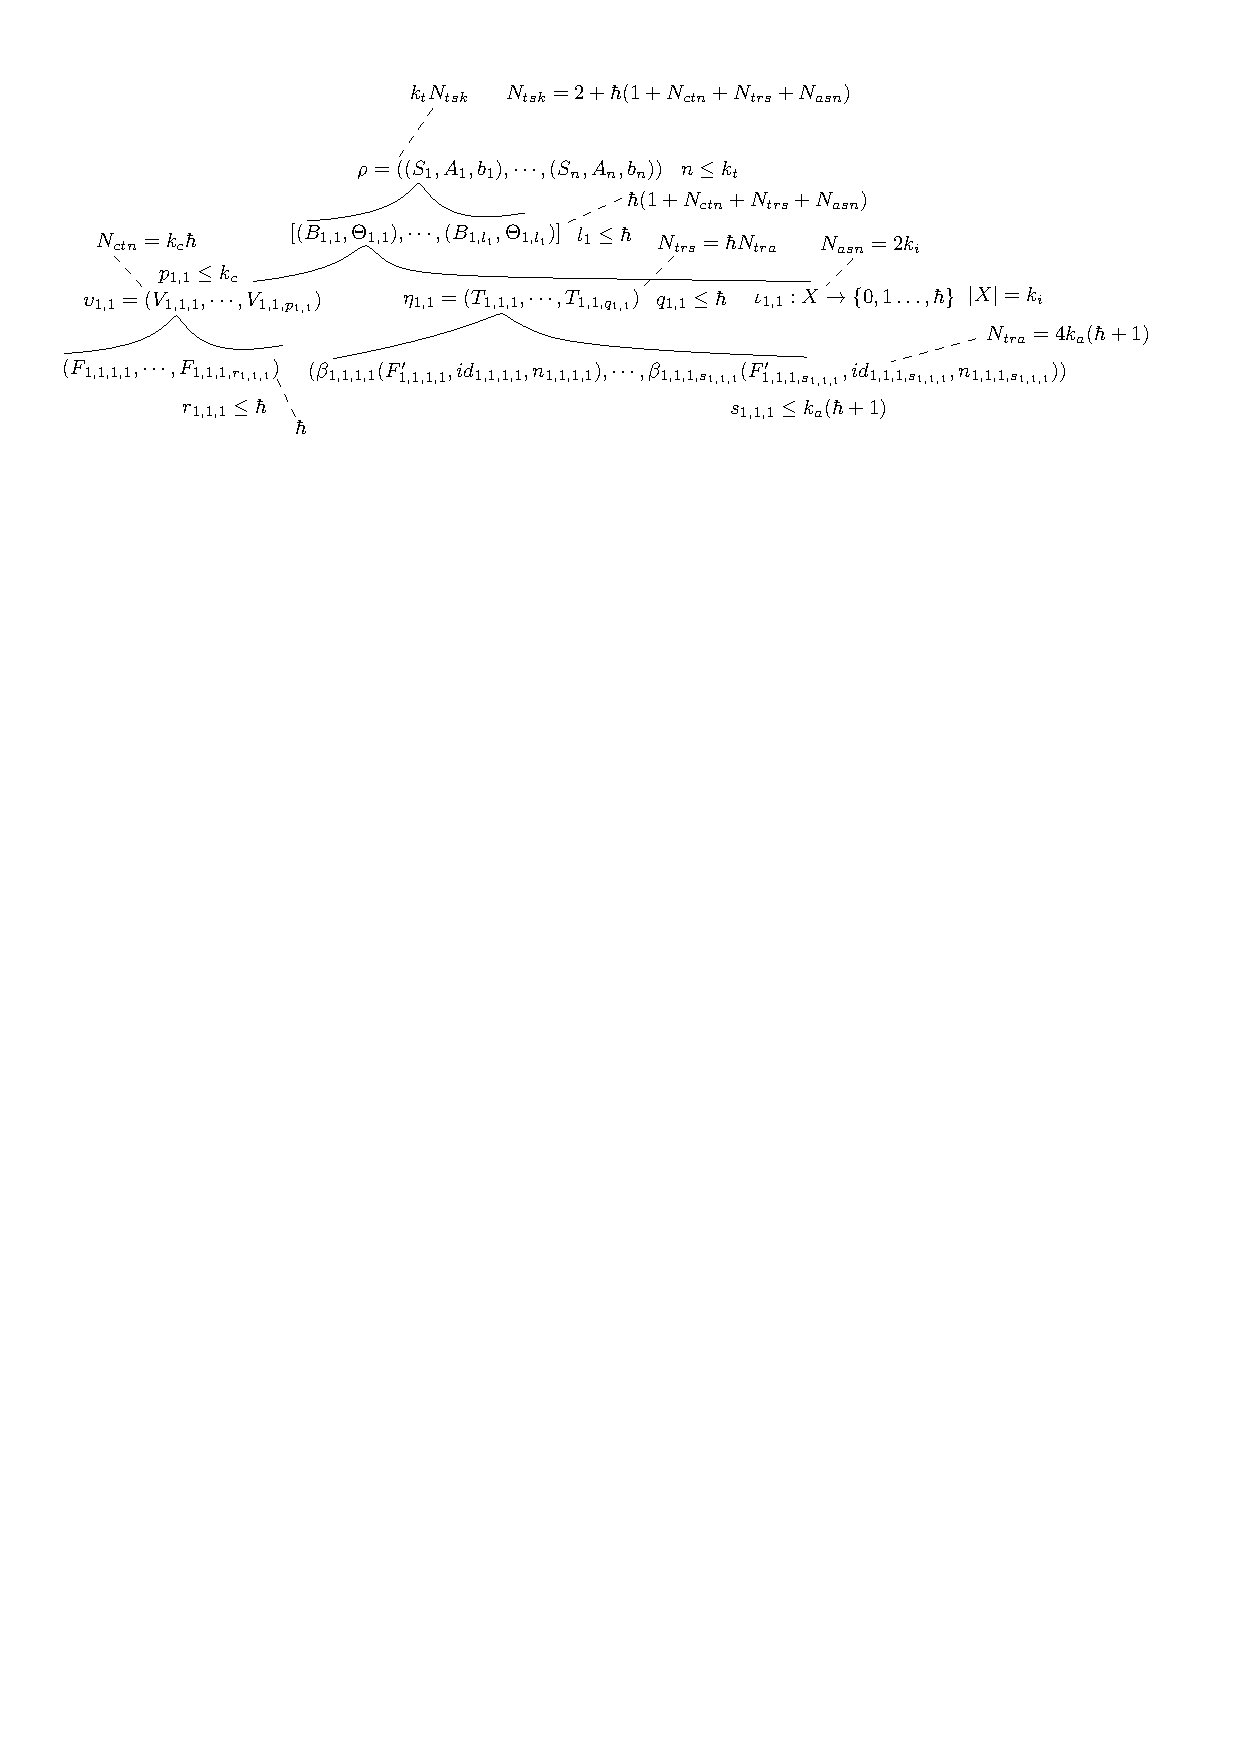
\includegraphics[scale = 0.7]{conf-enc-length.pdf}
\caption{Length of the word encoding a task stack}
\label{fig-conf-enc}
\end{figure*}

More specifically, we have that 
\begin{itemize}
\item each fragment container is encoded by a word of length $N_{ctn} =  k_c \hbar$, 
%
\item each transaction is encoded by a word of length $N_{tra} = 4k_a(\hbar+1)$, 
%
%\item $N_{tra} = 3k_a(\hbar+1)$ denote the length of the encoding of a transaction, 
\item each transaction stack is encoded by a word of length $N_{trs} = \hbar N_{tra}$, 
%
\item each assignment function is encoded by a word of length $N_{asn} = 2k_i $, i.e. a word of the form $x_1 n_1 \cdots x_{k_i} n_{k_i}$ (where $x_j \in X$ and $n_j \in \{0\} \cup [k_c\hbar]$), 
%
\item each activity is encoded by a word of length $N_{act} = 1+ N_{ctn} + N_{trs}+N_{asn}$, and
\item each task is encoded by a word of length $N_{tsk} =2+ \hbar N_{act}$.
\end{itemize}
Note that in the encoding, the top activity of the top task is in the first position.

We can then use $k_t N_{tsk}$ variables $X_1, \cdots, X_{k_t N_{tsk}}$ ranging over $\Sigma_\Mm$  to encode a task stack. 
Evidently, each symbol in $\Sigma_{\Mm}$ can be encoded as a bit vector of length $\log_2 |\Sigma_\Mm|$. For each $\sigma \in \Sigma_\Mm$, assume $\enc(\sigma)$ is the binary encoding of $\sigma$. 
Each configuration can be encoded by 
$
k_t N_{tsk} \log_2 |\Sigma_\Mm|
$
Boolean variables. 
%It follows that each configuration $(\rho, \ell)$ can be encoded by 
%$
%(k_t N_{tsk} +1) \log_2 |\Sigma_\Mm| 
%$
%Boolean variables. 
%
Therefore, $\Aa_\Mm$ uses $
k_t N_{tsk}  \log_2 |\Sigma_\Mm| 
$ state variables to encode the configurations in $\conf_{\Mm,c_t, \hbar}$. 
Moreover, $\Aa_\Mm$ contains the input variables to encode the transition rules of $\Mm$.
Equipped with these state variables and input variables, we then encode the semantics of the transition rules of $\Mm$ into the transitions of $\Aa_\Mm$. 
% 
%Then details of $\Aa_\Mm$ are omitted and can be found in Appendix~\ref{app-enc-amass-trans}. 


%%%%%%%%%%%%%%%%%%%%%%%%%%%%%%%%%%
%%%%%%%%%%%%%%%%%%%%%%%%%%%%%%%%%%



\section{Validation of the formal semantics} \label{sec:validation}
%!TEX root = main.tex

%We have defined the formal semantics of {\AMASS} models defined in Section~\ref{sec:amass}. 

The goal of this section is to validate the formal semantics of the {\AMASS} models defined in Section~\ref{sec:amass}.  
%to justify its correctness. 
To avoid tediousness, we focus on the two sub-models $\AOAMASS$ and $\FOAMASS$ of {\AMASS} %. Moreover, we focus on the validation of the formal semantics for 
and Android 13.0. 
%
We validate the formal semantics from two different perspectives. 
\begin{itemize}
\item At first, we audit the Java source code of Android operating system to extract the control flows of starting an activity and executing a fragment transaction respectively. We confirm that the formal semantics of {\AMASS} models defined in Section~\ref{sec:amass} indeed echo the extracted control flows. See Section~\ref{sec:val-code} for more about the code audit. 
%
\item Moreover, we select 21 Android apps to empirically validate the conformance of the formal semantics of {\AMASS} models to the actual behaviors of these apps in the Android operating system. The details of the empirical validation are given in Section~\ref{sec:val-exp}. 
\end{itemize}

%Recall that in Section~\ref{sec:amass}, we separate the concerns and define the semantics for the sub-models $\AOAMASS$ and $\FOAMASS$ and put the definition of the semantics of {\AMASS} in the appendix. To be consistent with the definition of the semantics, in the sequel, we show how to validate the semantics for $\AOAMASS$ and $\FOAMASS$ models, and put the validation of the semantics for {\AMASS} models in Appendix~\ref{app-sem-val-amass}. 

\subsection{Validation of the formal semantics by auditing the source code of Android OS}\label{sec:val-code}
%
%To validate the formal semantics by reviewing the Android source code, we only consider the two sub-models $\AOAMASS$ and $\FOAMASS$. 
%Since the Android source code is complicated, and the validation of the formal semantics of $\AOAMASS$ and $\FOAMASS$ is highly complicated. 
To validate the formal semantics of $\AOAMASS$ (resp. $\FOAMASS$), we trace the control flow of the Java source code\footnote{available at \url{https://android.googlesource.com/platform/frameworks/base/}.} starting from the procedure startActivity() (resp. commit()). %We focus on Android 13.0. 
%The source code are shown in Appendix~\ref{app:code-audit}.
We first consider $\AOAMASS$, then $\FOAMASS$. 
%Similarly, we trace the control flow when the procedure commit() is called to validate 
%To validate the formal semantics of $\AOAMASS$, we start from the function startActivity(), and trace the calls of functions, finally check whether the behavior of the back stack is consistent with the formal semantics. 
%Similarly, to validate the semantics of $\FOAMASS$, we start from the function commit(), finally check whether the behavior of the fragment stack and fragment transaction stack is consistent with the formal semantics.
%

\subsubsection{Auditing the source code of $\AOAMASS$}
Figure~\ref{fig:startActivity} shows the control flow starting from the procedure startactivity() in the Activity class, 
where the vertices represent the procedures in classes and edges represent the procedure calls. 

\begin{itemize}
\item Starting from startactivity(),  startActivityForResult() is called, then execStartActivity() is called, and so on, until the procedure startActivityInner() is reached, where the core control logic for starting an activity is implemented. 
%
\item In the procedure startActivityInner(), the following statements are executed sequentially: the procedure computeLaunchingTaskFlags(), a conditional statement where getReusableTask() and computeTargetTask() are in the two branches respectively, the procedure recycleTask(), and another conditional statement where setNewTask() and addOrReparentStartingActivity() are in the two branches respectively.  
%
\item The procedure getReusableTask() calls findTask(), in which the procedure process() is called, and process() calls the procedure forAllLeafTasks(), where the procedure test() is called. 
%
\item The procedure recycleTask() calls the procedure complyActivityFlags() and setNewTask() calls reuseOrCreateTask() respectively.
\end{itemize}
%\hide{
%    \begin{itemize}
%        \item in the Activity.java file, startActivity() function calls startActivityForResult() function in line 6043, then startActivityForResult() function calls execStartActivity() function of Instrumentation class in 6423,
%        \item in the Instrumentation.java file, execStartActivity() function calls startActivity() function of ActivityTaskManagerService class in line 1873,
%        \item in the ActivityTaskManagerService.java file, startActivity() function calls startActivityAsUser() function in line 1214, then startActivityAsUser() function calls execute() function in line 1288, we can see that execute() is a function of ActivityStarter class via line 1276 in ActivityTaskManagerService.java file and line 133 to line 135 in ActivityStartController.java file,
%        \item in the ActivityStarter.java file, execute() function calls executeRequest() function in line 742, and executeRequest() function calls startActivityUnchecked() function in line 1309, finally startActivityUnchecked() func calls startActivityInner() function in line 1479.
%    \end{itemize}
%}
\begin{figure}[htbp]
    % \vspace{-3mm}
        \centering
        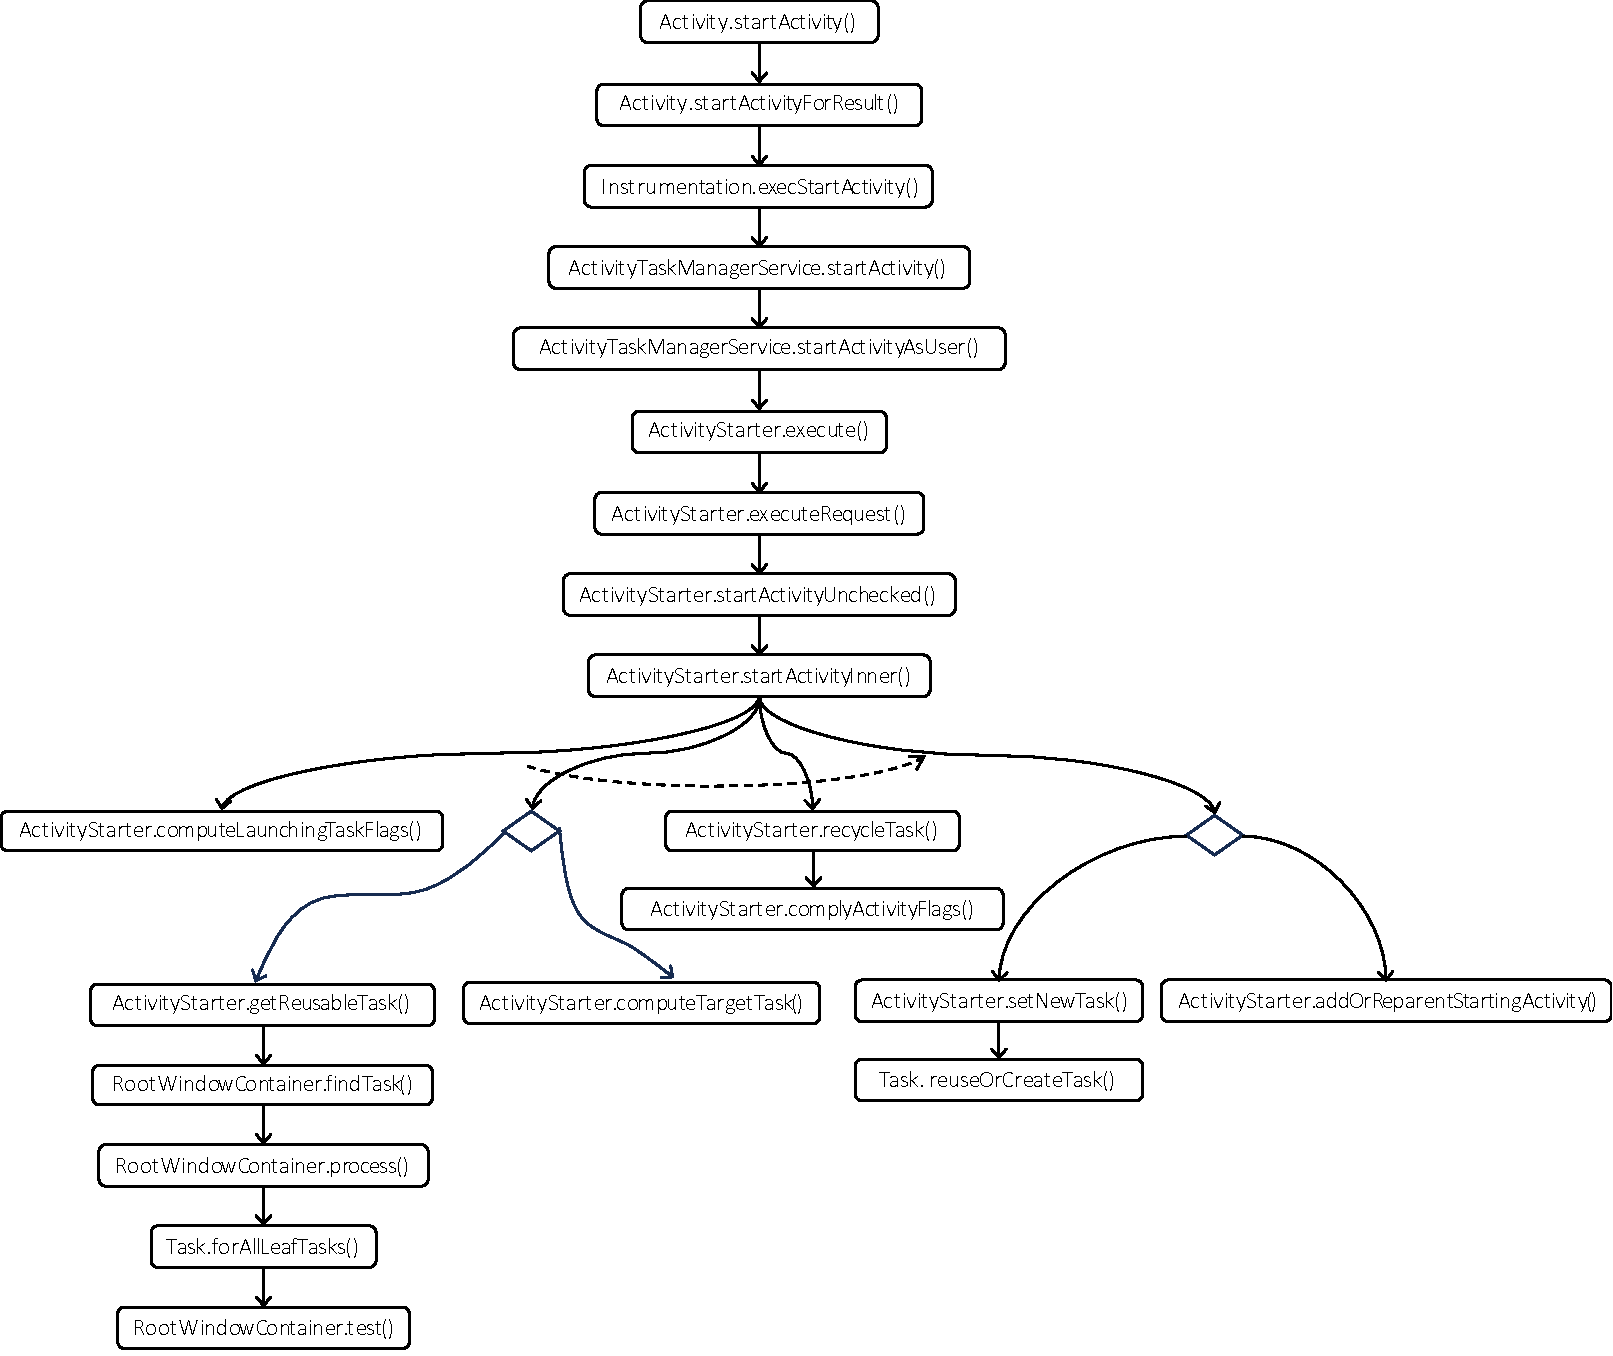
\includegraphics[scale = 0.55]{startActivity.pdf}
        \caption{Call graph for starting an activity}
            %in $\phi$
    % \vspace{-6mm}	
    \label{fig:startActivity}
\end{figure}

We audit the source code of the procedures called directly or indirectly by startActivityInner() and confirm that the semantics of $\AOAMASS$ is consistent with its actual implementation in Android OS. In particular, the task allocation mechanism and the intent flags in the semantics conform to the source code in Android OS.
The details of the auditing are relegated to Appendix~\ref{app:code-audit-aomass}. 

%%%%%%%%% the original text by Jinlong %%%%%%%
%%%%%%%%% the original text by Jinlong %%%%%%%
\hide{
Then it will call recycleTask() function in line 1716 to place $B$.
As shown in Code~\ref{code-recycleTask}, recycleTask() function actually calls complyActivityFlags() function in line 2090 to place $B$ in the task with the actual intent flags. 

    Recall that the formal semantics of $\AOAMASS$, there are three main steps for the evolution of the task stack by starting an activity $B$ from an activity $A$ as follows:
    \begin{enumerate}
        \item It will search for a task for $B$ according to the task allocation mechanism.
        \item Then it will place the activity $B$ in that task according to the intent flags, and the launch modes of $A$ and $B$,
    \end{enumerate}

\begin{itemize}
    \item As shown in Code~\ref{code-getReusableTask}, the getReusableTask() function in the ActivityStarter.java file will call findTask() function in line 2883 to search for a reusable task for the caller activity $B$. For each task in the task stack, findTask() will call test() function to check whether it is the target task. The test() function in the RootWindowContainer.java file will first check whether the real activity of the task matches the caller activity $B$ in line 392 (corresponding to the first step), then check whether the task affinity of the task matches the task affinity of the caller activity $B$ in line 399 (corresponding to the second step). 
    \item As shown in Code~\ref{code-setNewTask}, the setNewTask() function in the ActivityStarter.java file will create a new task for $B$ in line 3054(corresponding to the last step).
\end{itemize}



%search for a reusable target task in the task stack for the caller activity by calling getReusableTask() in line 1652 (corresponding to the first step) first. 
Then it will place the caller activity in the target task by calling recycleTask() in line 1709 (corresponding to the second step). 
    % Finally, if no such reusable task found, it will call setNewTask() in line 1734 to create a new task for the caller activity. Moreover, 

    Furthermore, recall that the task allocation mechanism, there are three steps:
    \begin{enumerate}
        \item If there is any task whose real activity is $B$, then $B$ will be put on the task. %(search downwards from the top task). 
        \item Otherwise, if there is any task whose real activity has the same \emph{task affinity} as $B$, then $B$ will be put on the task. %first such task (search downwards from the top task). 
        \item Otherwise, a new task is created to hold $B$. 
    \end{enumerate}
        In the first two steps, if there are multiple instances, the first occurrence starting from the top task will be selected. 
We confirm the task allocation mechanism by reviewing Code~\ref{code-getReusableTask} (corresponding to the first two steps) and Code~\ref{code-setNewTask} (corresponding to the last step). Moreover.
\begin{itemize}
    \item As shown in Code~\ref{code-getReusableTask}, the getReusableTask() function in the ActivityStarter.java file will call findTask() function in line 2883 to search for a reusable task for the caller activity $B$. For each task in the task stack, findTask() will call test() function to check whether it is the target task. The test() function in the RootWindowContainer.java file will first check whether the real activity of the task matches the caller activity $B$ in line 392 (corresponding to the first step), then check whether the task affinity of the task matches the task affinity of the caller activity $B$ in line 399 (corresponding to the second step). 
    \item As shown in Code~\ref{code-setNewTask}, the setNewTask() function in the ActivityStarter.java file will create a new task for $B$ in line 3054(corresponding to the last step).
\end{itemize}
% Finally, if no such reusable task found, getReusableTask() function will call setNewTask() function in line 1734, as shown in Code~\ref{code-setNewTask}, setNewTask() function will create a new task for the caller activity $B$ in line 3054 (corresponding to the third step).

Indeed, the combination of intent flag and launch modes of $A$ and $B$ has a collective impact on the placement of $B$. As shown in Code~\ref{code-startActivityInner}, startActivityInner() function will call the computeLaunchingTaskFlags() function in line 1636 to compute the actual intent flags via converting the launch modes to the intent flags. Then it will call recycleTask() function in line 1709 to place $B$.
As shown in Code~\ref{code-recycleTask}, recycleTask() function actually calls complyActivityFlags() function in line 2236 to place $B$ in the task with the actual intent flags. Moreover, recall that there are 4 ways to place $B$, i.e., $\clrtsk(\rho, B)$, $\clrtop(\rho, B)$, $\mvacttop(\rho, B)$ and $\push(\rho, B)$. The details of complyActivityFlags() function are shown as follows:
\begin{itemize}
    \item it will clear all activities in the task in line 2402 and push the caller activity $B$ into the task in line 2404 (corresponding to $\clrtsk(\rho, B)$),
    \item it will clear all activities above the caller activity $B$ in line 2414 (corresponding to $\clrtop(\rho, B)$),
    \item it will move the caller activity $B$ to the top of the task in line 2458 (corresponding to $\mvacttop(\rho, B)$),
    \item it will push the caller activity $B$ into the task directly in line 2495 (corresponding to $\push(\rho, B)$).
\end{itemize}

%
%    We confirm the behavior of the back stack is consistent with our formal semantics of $\AOAMASS$ defined in Section~\ref{sec:aoamass} by reviewing the Android source code. As shown in Code~\ref{scode-startActivity}, startActivity() function is involved to start an activity $B$ from $A$, 
%
    \begin{itemize}
        \item in the Activity.java file, startActivity() function calls startActivityForResult() function in line 6043, then startActivityForResult() function calls execStartActivity() function of Instrumentation class in 6423,
        \item in the Instrumentation.java file, execStartActivity() function calls startActivity() function of ActivityTaskManagerService class in line 1873,
        \item in the ActivityTaskManagerService.java file, startActivity() function calls startActivityAsUser() function in line 1214, then startActivityAsUser() function calls execute() function in line 1288, we can see that execute() is a function of ActivityStarter class via line 1276 in ActivityTaskManagerService.java file and line 133 to line 135 in ActivityStartController.java file,
        \item in the ActivityStarter.java file, execute() function calls executeRequest() function in line 742, and executeRequest() function calls startActivityUnchecked() function in line 1309, finally startActivityUnchecked() func calls startActivityInner() function in line 1479.
    \end{itemize}
    Consequently, startActivityInner() function in the ActivityStarter.java file deals with how to start $B$ in the back stack, the codes of startActivityInner() function are shown in Code~\ref{code-startActivityInner}.


Therefore, through reviewing Android source code, we discover that the behavior of the back stack shown in the source code is essentially consistent with the formal semantics of $\AOAMASS$.


% \begin{itemize}
% 	\item As shown in Code~\ref{code-getReusableTask}, 
%     getReusableTask() function will call findTask() function in line 2883 to search for a reusable task for the caller activity. For each task in the task stack, findTask() will call test() function shown in Code~\ref{code-test} to check whether it is the target task. 
% 	\item As shown in Code~\ref{code-recycleTask}, recycleTask() function will call complyActivityFlags() in line 2236 to place the caller activity in the target task. As shown in Code~\ref{code-complyActivityFlags}, complyActivityFlags() function will clear all activities in the target task and push the caller activity into the task in line 2420, or clear all activities above the caller activity in line 2432, or move the caller activity to the top of the target task in line 2474, or push the caller activity into the target task directly in line 2500, according to the launch modes of callee activity and caller activity, and the intent flags.
% 	\item As shown in Code~\ref{code-setNewTask}, setNewTask() function will create a task for the caller activity in line 3054.
% \end{itemize}
%\begin{lstlisting}[caption={The sample code for startActivity()},label={scode-startActivity}]
%    Intent intent = new Intent(A.this, B.class);
%    intent.setFlags(Intent.FLAG_ACTIVITY_NEW_TASK);
%    startActivity(intent);
%\end{lstlisting}

\begin{figure}[htbp]
\centering
\begin{tabular}{c}
%[basicstyle=\footnotesize\ttfamily]
\begin{lstlisting}
// +/master/core/java/android/app/Activity.java
6192    public void startActivity(Intent intent, @Nullable Bundle options) {
6193        getAutofillClientController().onStartActivity(intent, mIntent);
6194        if (options != null) {
6195            startActivityForResult(intent, -1, options);
                ...
6200        }
6201    }

// +/master/core/java/android/app/Activity.java
6571    public void startActivityForResult(
6572            String who, Intent intent, int requestCode, @Nullable Bundle options) {
            ...
6578        Instrumentation.ActivityResult ar =
6579            mInstrumentation.execStartActivity(
            ...
6588    }

// +/master/core/java/android/app/Instrumentation.java
1900    public ActivityResult execStartActivity(
1901            Context who, IBinder contextThread, IBinder token, Activity target,
1902            Intent intent, int requestCode, Bundle options) {
            ...
1941        try {
                ...
1944            int result = ActivityTaskManager.getService().startActivity(whoThread,
                ...
1952        }
            ...
1954    }

// +/master/services/core/java/com/android/server/wm/ActivityTaskManagerService.java
1233    public final int startActivity(IApplicationThread caller, String callingPackage,
                ...
1236            Bundle bOptions) {
1237        return startActivityAsUser(caller, callingPackage, callingFeatureId, intent, resolvedType,
            ...
1240    }

// +/master/services/core/java/com/android/server/wm/ActivityTaskManagerService.java
1274    private int startActivityAsUser(IApplicationThread caller, String callingPackage,
                ...
1277            ProfilerInfo profilerInfo, Bundle bOptions, int userId, boolean validateIncomingUser) {
            ...
1305        return getActivityStartController().obtainStarter(intent, "startActivityAsUser")
                    ...
1317                .execute();
1318    }
\end{lstlisting}
\end{tabular}
\caption{Android source code for responding to startActivity()}\label{code-startActivity-1}
\end{figure}

\begin{figure}[htbp]
\centering
\begin{tabular}{c}
\begin{lstlisting}
// +/master/services/core/java/com/android/server/wm/ActivityStartController.java
130    ActivityStarter obtainStarter(Intent intent, String reason) {
131        return mFactory.obtain().setIntent(intent).setReason(reason);
132    }

// +/master/services/core/java/com/android/server/wm/ActivityStarter.java
670    int execute() {
           ...
725                try {
                       ...
731                    res = executeRequest(mRequest);
                       ...
737                }
           ...
779    }

// +/master/services/core/java/com/android/server/wm/ActivityStarter.java
883     private int executeRequest(Request request) {
            ...
1315        mLastStartActivityResult = startActivityUnchecked(r, sourceRecord, voiceSession,
            ...
1324    }

// +/master/services/core/java/com/android/server/wm/ActivityStarter.java
1464    private int startActivityUnchecked(final ActivityRecord r, ActivityRecord sourceRecord,
                ...
1469            NeededUriGrants intentGrants, int realCallingUid) {
            ...
1481        try {
                ...
1486            result = startActivityInner(r, sourceRecord, voiceSession, voiceInteractor,
                ...
1496        }
            ...
1500    }
\end{lstlisting}
\end{tabular}
\caption{Android source code for responding to startActivity()}\label{code-startActivity-2}
\end{figure}
}
%%%%%%%%% the original text by Jinlong %%%%%%%
%%%%%%%%% the original text by Jinlong %%%%%%%



\hide{
\begin{lstlisting}[caption={Android system source code in RootWindowContainer.java file},label={activity-code-window}]
// platform_frameworks_base/blob/main/services/core/java/com/android/server/wm/RootWindowContainer.java
2833    Task getOrCreateRootTask(@Nullable ActivityRecord r,
2834        @Nullable ActivityOptions options, @Nullable Task candidateTask,
2835        @Nullable Task sourceTask, boolean onTop,
2836        @Nullable LaunchParamsController.LaunchParams launchParams, int launchFlags) {
2838        if (options != null) {
2839            final Task candidateRoot = Task.fromWindowContainerToken(options.getLaunchRootTask());
                ...
2843        }
            ...
2846        if (options != null) {
2847            final int candidateTaskId = options.getLaunchTaskId();
2848            if (candidateTaskId != INVALID_TASK_ID) {
                    ...
2851                final Task task = anyTaskForId(candidateTaskId,
2852                        MATCH_ATTACHED_TASK_OR_RECENT_TASKS_AND_RESTORE, options, onTop);
                    ...
2857            }
2858        }
            ...
2922        if (taskDisplayArea == null) {
2923            taskDisplayArea = getDefaultTaskDisplayArea();
2924        }
2925        return taskDisplayArea.getOrCreateRootTask(r, options, candidateTask, sourceTask,
2926                launchParams, launchFlags, activityType, onTop);
2927    }
\end{lstlisting}
}



%%%%%%%%%% FOAMASS
%%%%%%%%%% FOAMASS

\subsubsection{Auditing the source code for $\FOAMASS$}
\begin{figure}
    % \vspace{-3mm}
        \centering
        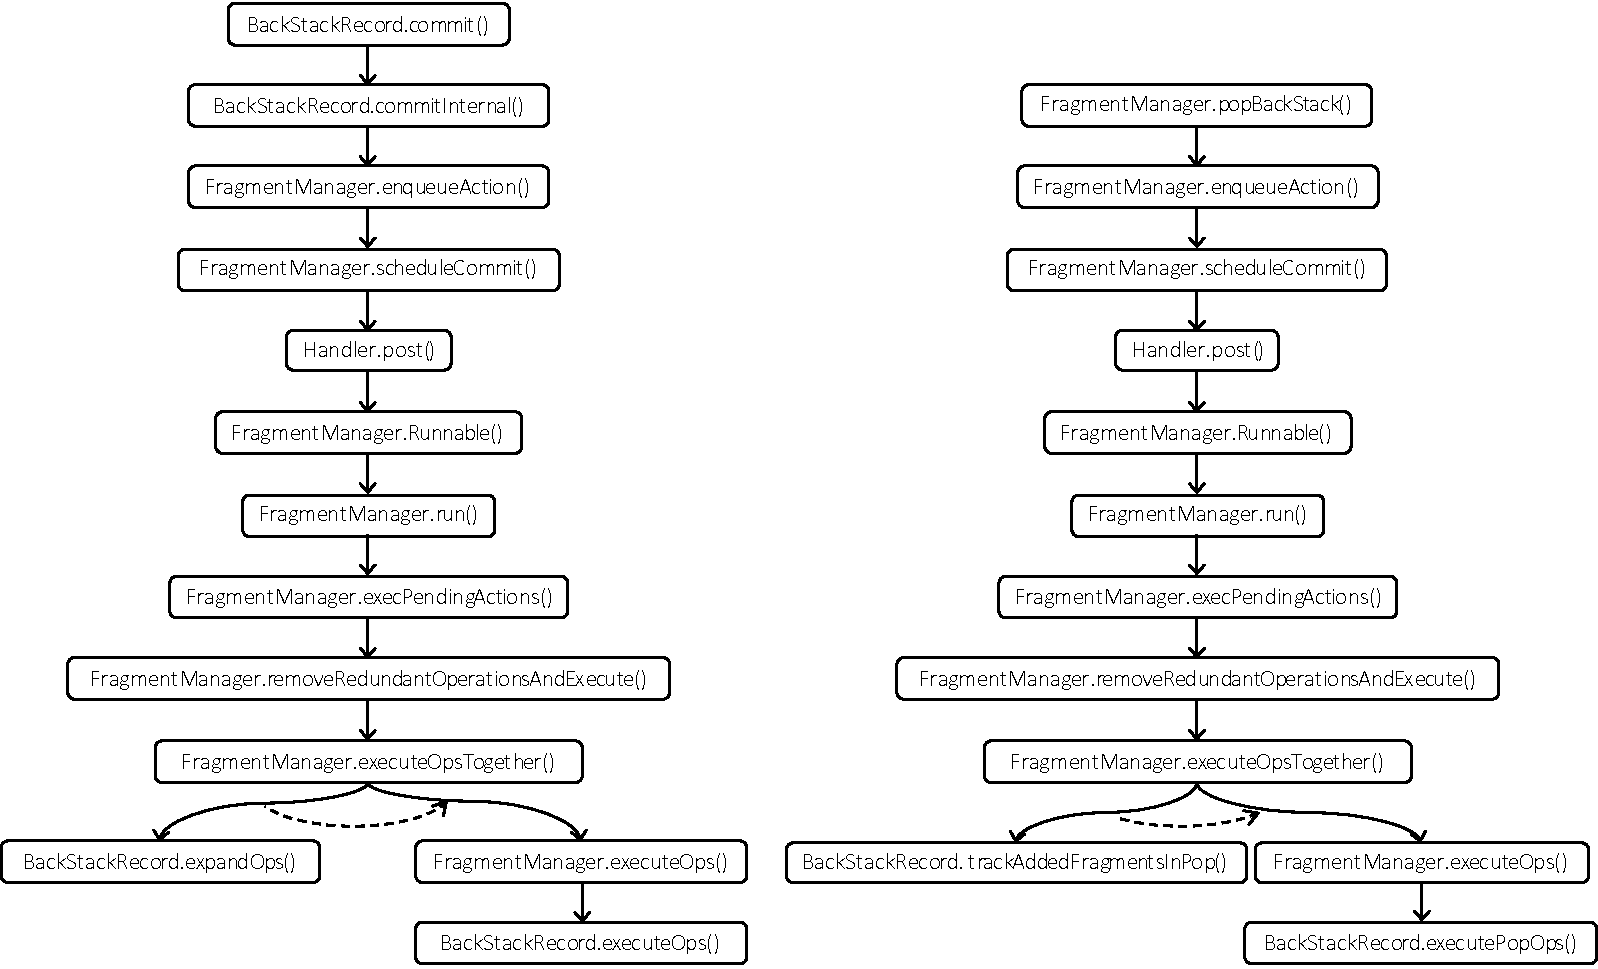
\includegraphics[scale = 0.55]{commit.pdf}
        \caption{Call graphs for committing and popping a fragment transaction}
            %in $\phi$
    % \vspace{-6mm}	
    \label{fig:commit}
\end{figure}

The control flows of committing and popping a fragment transaction are illustrated in Figure~\ref{fig:commit}. 
\begin{itemize}
\item We start with committing a fragment transaction first. From Figure~\ref{fig:commit}, to commit a fragment transaction, commit() is called. Then it calls commitInternal(), which calls enqueueAction() and so on  until executeOpsTogether() is called, where the core control logic for committing a fragment transaction is implemented. The procedure executeOpsTogether() calls expandOps() first, then executeOps(). Finally, executeOps() calls BackStackRecord.executeOps(). 
%
\item The call graph for popping a fragment transaction is similar. From Figure~\ref{fig:commit}, to pop a fragment transaction, popBackStack() is called. Then it calls commitInternal(), which calls enqueueAction() and so on  until executeOpsTogether() is called. The procedure executeOpsTogether() calls trackAddedFragmentsInPop() first, then executeOps(). Finally, executeOps() calls BackStackRecord.executePopOps(). 
\end{itemize}

We audit the source codes of the procedure executeOpsTogether() as well as those called by it directly or indirectly and confirm that 
\begin{itemize}
\item the way of dealing with REP actions in the semantics of $\FOAMASS$ in Section~\ref{sec-foamass} is consistent with the source code of expandOps(), 
\item the execution of fragment actions as defined in the semantics of $\FOAMASS$ in Section~\ref{sec-foamass} is consistent with the source code of BackStackRecord.executeOps(),
\item the way of revoking fragment transactions in the semantics of $\FOAMASS$ in Section~\ref{sec-foamass} is consistent with the source code of trackAddedFragmentsInPop(). 
\end{itemize}
The details of the auditing are relegated to Appendix~\ref{app:code-audit-fomass}.


%%%%%%%%%% original texts by Jinlong
%%%%%%%%%% original texts by Jinlong
\hide{
Moreover, from line 914 to line 932, the "remove" action of each fragment from the fragment stack will be pushed into fragment transaction sequentially, and the "add" action will be pushed into the fragment transaction in line 932.

As shown in Code~\ref{code-execute}, expandOps() is used to expand the fragment transaction, executeOps() is used to execute the fragment actions sequentially of the expanded fragment transaction, Moreover,
\begin{itemize}
    \item expandOps() function expands the fragment transaction by converting the fragment action "replace" into a sequence of fragment actions, consisting only of "add" and "remove" actions. Moreover, from line 914 to line 932, the "remove" action of each fragment from the fragment stack will be pushed into fragment transaction sequentially, and the "add" action will be pushed into the fragment transaction in line 932.
    Therefore, it is consistent with our formal semantics of $\REP$ of $\FOAMASS$.
    \item executeOps() function executes the fragment actions sequentially of the expanded fragment transaction. From line 768 to line 775, we can see that it only executes the "add" and "remove" actions, since there is no "replace" action in the fragment transaction which is expanded by expandOps() function. Moreover, it push (resp. remove) the fragment into (resp. from) the fragment stack when executing "add" (resp. "remove") action in line 770 (resp. 774).
    Therefore, it is consistent with our formal semantics of $\ADD$ and $\REM$ of $\FOAMASS$.
\end{itemize}

We confirm the behavior of the fragment stack and fragment transaction back stack is consistent with our formal semantics of $\FOAMASS$ defined in Section~\ref{sec-foamass} by reviewing the Android source code. As shown in Code~\ref{scode-fragtran}, commit() function is involved to execute the fragment transaction $ft$, Code~\ref{code-commit} shows a series of function calls to respond to function commit(). Moreover,
\begin{itemize}
    \item in the BackStackRecord.java file, commit() function calls the commitInternal() function in line 646, then commitInternal() function calls enqueueAction() function of FragmentManager class in line 688.
    \item in the FragmentManager.java file, enqueueAction() function defined in line 1903 calls scheduleCommit() function in line 1919, then scheduleCommit() function calls post(mExecCommit) function to call Runnable() function in line 739, then it calls execPendingActions() function in line 743, then execPendingActions() function calls removeRedundantOperationsAndExecute() function in line 2067, then it calls executeOpsTogether() function in line 2166. Finally executeOpsTogether() function calls expandOps()  function of BackStackRecord class in line 2193 and executeOps() function in line 2205 which calls executeOps() function of BackStackRecord class in line 2410.
\end{itemize}
Consequently, there are two functions of BackStackRecord class, i.e., expandOps() and executeOps() responding the commit() function.

Furthermore, $\back$ action will cancel the effects of the top fragment transaction of the fragment transaction stack if stack is not empty. As shown in Code~\ref{code-commit}, the popBackStack() in FragmentManager.java will be involved, then it will call enqueueAction() function. Similarly, it will call executeOpsTogether() finally, the difference is that it will call trackAddedFragmentsInPop() function in line 2195 instead of expandOps() function. Moreover, when executeOpsTogether() calls the executeOps() function in line 2205, the parameters isRecordPop is set true, hence executeOps() function will call executePopOps() function in 2407 instead of executeOps(). As shown in Code~\ref{code-execute}, trackAddedFragmentsInPop() function will not convert any action, since there are only "add" and "remove" actions in the fragment transaction. The executePopOps() function will execute the reverse actions of the fragment actions in the fragment transaction sequentially, for example, it will execute "remove" (resp. "add") action, if there is a "add" (resp. "remove") action in the fragment transaction. In this way, the effects of the fragment transaction will be cancelled which is consistent with our formal semantics of $\FOAMASS$.

Therefore, through reviewing Android source code, we discover that the behavior of the fragment stack and fragment transaction stack shown in the source code is essentially consistent with the formal semantics of $\FOAMASS$.

\begin{lstlisting}[caption={The sample code for FragmentTransaction},label={scode-fragtran}]
    Fragment F1 = new Fragment1();
    Fragment F2 = new Fragment2();
    FragmentTransaction ft = getFragmentManager().beginTransation();
    ft.add(R.id, F1);
    ft.replce(R.id, F2);
    ft.remove(F2);
    ft.addToBackStack("");
    ft.commit();
\end{lstlisting}
%
\begin{lstlisting}[caption={Android source code for responding add(), replace(), remove() and addToBackStack()},label={code-add}]
// core/java/android/app/BackStackRecord.java
173     final class BackStackRecord extends FragmentTransaction implements
174             FragmentManager.BackStackEntry, FragmentManagerImpl.OpGenerator {
            ...
413         public FragmentTransaction add(int containerViewId, Fragment fragment) {
414             doAddOp(containerViewId, fragment, null, OP_ADD);
                ...
416         }
            ...
423         private void doAddOp(int containerViewId, Fragment fragment, String tag, int opcmd) {
                ...
455             fragment.mContainerId = fragment.mFragmentId = containerViewId;
                ...
458             addOp(new Op(opcmd, fragment));
459         }
            ...
465         public FragmentTransaction replace(int containerViewId, Fragment fragment) {
                ...
470             doAddOp(containerViewId, fragment, tag, OP_REPLACE);
                ...
472         }
            ...
474         public FragmentTransaction remove(Fragment fragment) {
475             addOp(new Op(OP_REMOVE, fragment));
                ...
478         }
            ...
555         public FragmentTransaction addToBackStack(String name) {
                ...
560             mAddToBackStack = true;
                ...
563         }
            ...
1024    }
\end{lstlisting}

\begin{lstlisting}[caption={Android source code for responding commit() and popBackStack()},label={code-commit}]
// +/master/core/java/android/app/BackStackRecord.java
645     public int commit() {
646         return commitInternal(false);
647     }

// +/master/core/java/android/app/BackStackRecord.java
671     int commitInternal(boolean allowStateLoss) {    
            ...
683         if (mAddToBackStack) {
684             mIndex = mManager.allocBackStackIndex(this);    
                ...
687         }
688         mManager.enqueueAction(this, allowStateLoss);    
        ...
690     }

// +/master/core/java/android/app/FragmentManager.java
739     Runnable mExecCommit = new Runnable() {
740         @Override
741         public void run() {
742             execPendingActions();
743         }
744     };

// +/master/core/java/android/app/FragmentManager.java
828     public void popBackStack() {
829     enqueueAction(new PopBackStackState(null, -1, 0), false);
830     }

// +/master/core/java/android/app/FragmentManager.java
1903    public void enqueueAction(OpGenerator action, boolean allowStateLoss) {
            ...
1919        scheduleCommit();
            ...
1921    }

// +/master/core/java/android/app/FragmentManager.java
1929    private void scheduleCommit() {
            ...
1936        mHost.getHandler().post(mExecCommit);
            ...
1939    }

// +/master/core/java/android/app/FragmentManager.java
2060    public boolean execPendingActions() {
            ...
2067        removeRedundantOperationsAndExecute(mTmpRecords, mTmpIsPop);
            ...
2078    }

// +/master/core/java/android/app/FragmentManager.java
2128    private void removeRedundantOperationsAndExecute(ArrayList<BackStackRecord> records,
2129            ArrayList<Boolean> isRecordPop) {
            ...
2166        executeOpsTogether(records, isRecordPop, startIndex, numRecords);
            ...
2168    }

// +/master/core/java/android/app/FragmentManager.java
2178    private void executeOpsTogether(ArrayList<BackStackRecord> records,
2179            ArrayList<Boolean> isRecordPop, int startIndex, int endIndex) {
            ...
2192        if (!isPop) {
2193            oldPrimaryNav = record.expandOps(mTmpAddedFragments, oldPrimaryNav);
2194        } else {
2195            record.trackAddedFragmentsInPop(mTmpAddedFragments);
2196        }
            ...
2205        executeOps(records, isRecordPop, startIndex, endIndex);
            ...
2236    }

// +/master/core/java/android/app/FragmentManager.java
2397    private static void executeOps(ArrayList<BackStackRecord> records,
2398            ArrayList<Boolean> isRecordPop, int startIndex, int endIndex) {
            ...
2402        if (isPop) {
                ...
2407            record.executePopOps(moveToState);
2408        } else {
                ...
2410            record.executeOps();
2411        }
            ...
2413    }

\end{lstlisting}
}
%%%%%%%%%% original texts by Jinlong
%%%%%%%%%% original texts by Jinlong



\subsection{Empirical validation of the formal semantics}\label{sec:val-exp}

To validate the semantics of $\AOAMASS$ empirically, we select 10 apps from F-Droid. These apps are selected to cover as many launch modes and intent flags as possible.  Similarly, to validate the semantics of $\FOAMASS$, we select 10 apps from F-Droid to cover as many types of fragment transactions as possible. Nevertheless, these apps are far from covering the vast number of cases in the definition of the semantics of $\AOAMASS$ and $\FOAMASS$, since there are exponentially many different combinations of intent flags. 
% \jinlong{the main reason is that the intent flags may interfere with each other. For example, $\ctpflag$ will be ignored when $\ctkflag$ is set, hence real world apps may not use $\ctkflag$ and $\ctpflag$ together. However, we need to validate all possible combinations of intent flags to ensure the correctness of the semantics of $\AOAMASS$, even though most combinations are not used in the real world apps.}
Therefore, in addition to these apps, we design a special Android app, called ``ValApp'', aiming at covering all the cases in the definition of the semantics of $\AOAMASS$ and $\FOAMASS$ models. 

The reason that we only select 10 apps from F-Droid plus ValApp to validate the semantics of $\AOAMASS$ (resp. $\FOAMASS$), instead of validate the semantics by experimenting on a large pool of existing apps, lies in the fact that although we shall propose an automated method for semantics validation in Section~\ref{sec-aut-val}, it is hard to apply the automated method to a large number of existing apps,  since generating sequences of click events for transitions is still a manual process. As a result, we mainly rely on ValApp to fulfill the semantics validation. We would like to argue that using ValApp to fulfill the semantics validation does not affect very much the soundness since after the options e.g. launch modes and intent flags are chosen, the rest of the validation process is the same as real-world Android apps, that is, the startActivity() procedure is executed in the Android OS and the results are collected and compared. 

A snapshot of the ValApp is shown in Figure~\ref{fig:valapp}. 
ValApp\footnote{available at https://github.com/Jinlong-He/ValApp/tree/main} includes 8 activities, corresponding to the $8$ (launch mode, task affinity) pairs from $\{\STD, \STP, \STK, \SIT\} \times \{1,2\}$. Moreover, ValApp provides means to choose the launch modes and intent flags, as well as ``start'' and ``finishStart'', so that transition rules can be generated for all their combinations. 
Furthermore, each activity of ValApp includes two fragments and two fragment containers. It also provides two variables for fragment identifiers and allows arbitrary combinations of actions to form fragment transactions. Finally, ValApp allows pushing arbitrarily many transactions into the fragment transaction stack. 
%
From the design, we can see that ValApp is capable of comprehensively accounting for all factors that may affect the semantics of $\AOAMASS$ and $\FOAMASS$ models. Moreover, we ValApp is \emph{universal} in the sense that a user can interact with ValApp to choose the transition rules and generate a desired {\AMASS} model. 

%two fragment containers, for each activity. For each transition, ValApp can provide any combination of actions and combine them into fragment transactions of any length.

%two activities  each launch mode corresponds to two distinct activities with different affinities. For each transition, ValApp allows for any combination of intent flags and launch modes and the option to select "start" or "finishStart".
%ValApp also offers two fragments and two fragment containers for each activity. For each transition, ValApp can provide any combination of actions and combine them into fragment transactions of any length.

\begin{figure}[htbp]
\centering
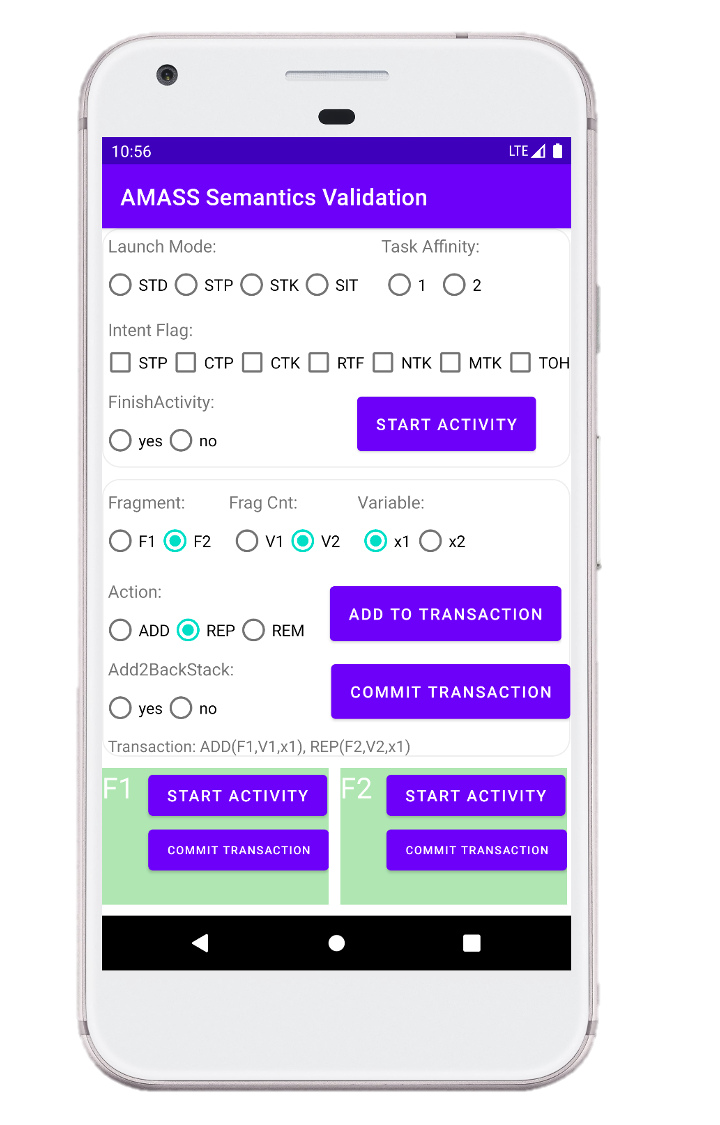
\includegraphics[scale=0.5]{ValApp.png}
\caption{ValApp: An Android app designed for validating the semantics of $\AMASS$}
\label{fig:valapp}
\end{figure}


%As shown in Figure~\ref{fig:valapp}, ValApp offers 8 selectable activities, where each launch mode corresponds to two distinct activities with different affinities. For each transition, ValApp allows for any combination of intent flags and launch modes and the option to select "start" or "finishStart".
%ValApp also offers two fragments and two fragment containers for each activity. For each transition, ValApp can provide any combination of actions and combine them into fragment transactions of any length.
%Therefore, by providing a range of selectable activities, different combinations of the intent flags, and customizable fragment transactions, ValApp is able to comprehensively account for all factors that may affect the semantics of the Android system.


%In this section, we validate the formal semantics of {\AMASS} models defined in Section~\ref{sec:amass} against the actual behavior of  Android apps.  To facilitate the validation, we selected $10$ apps from F-Droid , which cover as many launch modes, intent flags (resp. fragment transactions) as possible. (Note that we select apps from F-Droid because these open-source apps enable more accurate experimentation.)Because of the complicated  semantics, especially a vast number of possible combinations of launch modes and intent flags, real-world applications may not cover  all possible cases. To address this issue, we design an Android app “AMASS Semantics Validation” (abbreviated as ValApp) to facilitate the validation.

% Since the semantics are highly complicated, especially the number of the combinition of the launch modes and the intent flags is large, the real-world apps could not cover all the cases of the semantics, hence we design an Android app “AMASS Semantics Validation” (abbreviated as ValApp) to supplement the validation. 
% As shown in Figure 7, ValApp contains the following UI widgets.

% To facilitate the validation, we design an Android app   ``AMASS Semantics Validation'' (abbreviated as ValApp). 
%
%
% where radio buttons/check boxes for launch modes, task affinities, intent flags, fragments, fragment containers, and fragment transactions etc. are provided to generate the transition rules of {\AMASS} models. One the choices are made and a transition rule is generated, the transition rule can be executed by clicking the ``START ACTIVITY'' button or ``COMMIT TRANSACTION'' button, and the task stack will be updated. 
%
%
%Specifically, 
%As shown in Figure~\ref{fig:valapp}, ValApp offers 8 selectable activities, where each launch mode corresponds to two distinct activities with different affinities. For each transition, ValApp %allows for any combination of intent flags and launch modes and the option to select "start" or "finishStart".
%ValApp also offers two fragments and two fragment containers for each activity. For each transition, ValApp can provide any combination of actions and combine them into fragment transactions of any length.
%Therefore, by providing a range of selectable activities, different combinations of the intent flags, and customizable fragment transactions, ValApp is able to comprehensively account for all factors that may affect the semantics of the Android system.

% ValApp could apply any combinition of the launch modes and the intent flags for the transitions, 
% ValApp contains the following UI widgets.
%\hide{
%\begin{itemize}
%\item Eight activities, one for each pair (launch mode, task affinity), where the launch modes are from the set $\{\standard, \singletop, \singletask, \singleinstance\}$ and the task affinities are from $\{1, 2\}$. Moreover, it contains the following radio buttons and check boxes for the transition rules to start activities. 
%\begin{itemize}
%\item ValApp contains the radio buttons for choosing the launch modes and task affinities (1 or 2). Once the launch mode and task affinity are chosen, the activity of the corresponding launch mode and task affinity will be launched when the ``START ACTIVITY'' button is pressed. 
%%
%\item  ValApp contains eight check boxes, one for each intent flag, so that the intent flags can be configured to be valid or not. 
%%
%\item ValApp contains a radio button for choosing whether to finish the top activity or not, namely, whether a $\startactivity$ or $\finishstart$ transition rule will be executed. 
%\end{itemize}
%%
%\item ValApp contains two fragments $F_1, F_2$ and two fragment containers $V_1, V_2$. It also contains the following radio buttons for the transition rules to start fragment transactions.
%%
%\begin{itemize}
%\item ValApp contains the radio buttons for configuring fragment actions, i.e. the buttons for choosing $\{\ADD, \REP, \REM\}$, the fragments from $\{F_1, F_2\}$, the fragment containers from $\{V_1, V_2\}$, and the variables from $\{x_1, x_2\}$ to store the identifiers of fragment instances. Once a fragment action is configured, it can be added to a fragment transaction by clicking the ``ADD TO TRANSACTION'' button.
%%
%\item After adding all the actions to the current fragment transaction, the ``ASS2BackStack'' radio button can be used to choose whether to add the transaction into the fragment transaction stack.
%%
%\item When the configuration of a fragment transaction is complete, the ``COMMIT TRANSACTION'' button can be pressed to execute the actions in the transaction and update the fragment containers and fragment transaction stack. 
%%
%\end{itemize}
%\item Furthermore, the bottom of the ValApp window contains two copies of ``START ACTIVITY'' and ``COMMIT TRANSACTION'' buttons, corresponding to the transition rules of the form $F_i \xrightarrow{\alpha(\phi)} B$ and $F_i \xrightarrow{\mu} T$ ($i = 1,2 $).
%\end{itemize}
%}

%\tl{is this sentence finished?}
%Note that ValApp is a special app designated to do 

Nevertheless, manual validation the formal semantics for all different cases and different Android versions is a daunting task. %, since the number of cases in the definition of the semantics is huge. Therefore, in the sequel, 
Therefore, we propose an automated method %of automatically validating the formal semantics 
by utilizing %the symbolic model checker 
the nuXmv model checker, the Android UIAutomator testing framework, and the ADB tool. 

Let us focus on Android 13.0 in this section and validate the semantics of $\AOAMASS$ and $\FOAMASS$ models under this version. 
The verification of the formal semantics of $\AOAMASS$ and $\FOAMASS$  under the other versions is similar and omitted. 


%ValApp will be used as an example to describe the experiment. Then for each Android version from 7.0, 8.0, 9.0, 10.0, 11.0, 12.0, we validate the formal semantics against the actual behaviors of Android multitasking mechanism as follows. We enumerate all the cases in the semantics definition one by one, and for each case, validate the compatibility of the formal semantics with the actual behaviors of the ValApp. 

%\revision{Our semantics validation experiment is divided into three parts. Firstly, we validate the semantics of $\AOAMASS$ and $\FOAMASS$ separately. Then, we combine the above two experiments to validate the complete version of semantics.  }


\subsubsection{Automated method for semantics validation}\label{sec-aut-val}

Let $X$ be an Android app and $\Mm$ be an $\AOAMASS$ (resp. $\FOAMASS$) model that is extracted from $X$ and $\Aa$ be the nuXmv FSM model that encodes the configuration reachability problem of $\Mm$, where $c_t$, the bound on the number of tasks of the same affinity, and $\hbar$, the bound on the height of the stacks, are set to be $2$ and $6$ respectively. 
%We let $c_t  = 2$ and $\hbar = 6$ here, since in this case we assume that there is no fragments in activity, hence we have $k_a=0$. 
Moreover, $k_a$, the number of actions in one fragment transaction, is set to be $2$. 
%With the bounds $c_t, k_a, \hbar$, $\Mm$ is encoded by a nuXmv FSM model $\Aa$. 


The automated method to validate the semantics goes as follows. For a transition rule $\tau$,  
\begin{enumerate}
\item we use nuXmv to search for a path $\pi = \pi_1 \cdots \pi_m$ in $\Aa$, where an accepting condition corresponding to $\tau$ is set, in order to reach a configuration where $\tau$ can be applied (in other words, $\tau$ is enabled by the configuration), 
%that $A$ is the top activity of $S_1$, there is $i$ such that $i \neq 1$, $A_i = B$ and $i$ is the minimum such index, moreover, $B$ occurs in $S_i$ and $B$ is not the top activity of $S_i$ and $\zeta_i \neq \mainflag $. 
%
\item we generate from the app $X$ and each transition $\pi_i$ with $i \in [m]$, a sequence of click events in $X$, say $e_i$,
%
\item we use UIAutomator to execute the click events in $e_1, \cdots, e_m$ one by one (the task stack is updated), moreover, after the execution of all the click events, we use ADB to extract the resulting configuration, that is, the contents of the resulting task stack, say $\rho$,  

\item we generate the sequence of click events in $X$, say $e$, to fulfill the application of the transition rule  $\tau$,   
%
% \item Then for each $\phi \models \neg \tohflag \wedge \ntkflag \wedge \neg \mtkflag \wedge \rtfflag \wedge \neg \ctpflag \wedge \neg \ctkflag $, namely, for $\phi_0 = \neg \tohflag \wedge \ntkflag \wedge \neg \mtkflag \wedge \rtfflag \wedge \neg \ctpflag \wedge \neg \ctkflag \wedge \neg \stpflag$ and $\phi_1 = \neg \tohflag \wedge \ntkflag \wedge \neg \mtkflag \wedge \rtfflag \wedge \neg \ctpflag \wedge \neg \ctkflag \wedge \stpflag$, we generate two sequences of click events, say $e'_0, e'_1$, for two transition rules $\tau_0 = A \xrightarrow{\startactivity(\phi_0)} B$ and $\tau_1 = A \xrightarrow{\startactivity(\phi_1)} B$, that describe the selection of the launch mode and task affinity of $B$, the check boxes for intent flags, the FinishActivity option, and finally the operation of clicking the ``START ACTIVITY'' button.  
%
% \item We use UIAutomator again to execute the click events in $e'_0$ (resp. $e'_1$) one by one, and use ADB to obtain the resulting configuration $\rho'_0$ (resp. $\rho'_1$). Let $\tau_0(\rho)$ (resp. $\tau_1(\rho)$) denote the expected configuration obtained by applying $\tau'_0$ (resp. $\tau'_1$) on $\rho$ according to the formal semantics. If $\tau_0(\rho) \neq \rho'_0$ or $\tau_1(\rho) \neq \rho'_1$, then report that the formal semantics of {\AMASS} models and the actual semantics of Android multitasking mechanism are different. 
\item we use UIAutomator again to execute the click events in $e$ one by one, and use ADB to obtain the resulting configuration $\rho'$,
%
\item if $\rho' \neq \tau(\rho)$, then report the semantic inconsistency, where 
$\tau(\rho)$ denotes the expected configuration obtained by applying $\tau$ on $\rho$ according to the formal semantics. 
%If $\tau(\rho) \neq \rho'$, then report that the formal semantics of {\AMASS} models and the actual semantics of Android multitasking mechanism are different.
\end{enumerate}
Note that the semantics validation method is automated in the sense that it can automatically execute the sequences of click events and compare the resulting configurations, but the sequences of click events should still be \emph{manually} generated. This partially explains why we choose only 20 real-world apps to validate the semantics and mainly relies on ValApp to fulfill the validation. 

%Note that in the aforementioned automated semantics validation method, the generation of sequences of click events in the app $X$ is manually done. As a result, 

%\revision{
\subsubsection{Validation of the formal semantics of $\AOAMASS$}
%
To valid the semantics, we consider the transition rules of the form $\tau = A\xrightarrow{\alpha(\phi)} B$, and generate one configuration for each combination of the launch modes of $A$ and $B$, the values of $\alpha$, the intent flags, and the constraints on the configuration before applying the transition, e.g. $\getrealtsk(\rho, B) = *$, $\gettsk(\rho, B) = S_1$, and $\topact(\rho) = B$. 
In total, there are $901,120$ different combinations to be considered and we would like to generate configurations for all of them.


%%%%%%%%%%%%%%%%%%%%%%%%%%%%%%%%%%%%%%%%%%%%%%%%%%%%%%%%%%%%
%%%%%%%%%%%%%%%%%%%%%%%%%%%%%%%%%%%%%%%%%%%%%%%%%%%%%%%%%%%%
\hide{
In order to validate semantics and avoid overfitting, we enumerated the launch modes of $A$ and $B$, the intent flags $\phi$ and the cases of the configurations $(\rho, b)$ where $\rho = ((S_1,A_1,\zeta_1),\cdots,(S_k,A_k,\zeta_k))$ for $\rho\xrightarrow[\tau]{\Mm}\rho'$ and $\tau = A\xrightarrow{\alpha(\phi)}B$.
\begin{enumerate}
    \item Launch modes: There are $4\times 4=16$ possible combinations of launch modes for $A$ and $B$. 
    % \item Start modes: There are $2$ cases of $\alpha$, i.e., $\startactivity$ and $\finishstart$.
    \item Intent flags: There are $2^{10}=1,024$ possible combination of the intent flags $\phi$.
    \item Configuration: According to the task allocation mechanism, we know there are $5$ cases,
    \begin{itemize}
        \item $\getrealtsk(\rho, B) = S_1$ and $\zeta_1 = \mainflag$,
        \item $\getrealtsk(\rho, B) = S_i$, $i > 1$ and $\zeta_i = \mainflag$,
        \item $\getrealtsk(\rho, B) = S_1$ and $\zeta_1 \neq \mainflag$,
        \item $\getrealtsk(\rho, B) = S_i$, $i > 1$ and $\zeta_i \neq \mainflag$,
        \item $\getrealtsk(\rho, B) = * \wedge \gettsk(\rho, B) = S_1$,
        \item $\getrealtsk(\rho, B) = * \wedge \gettsk(\rho, B) = S_i$, $i > 1$,
        \item $\gettsk(\rho, B) = *$,
    \end{itemize}
    and for the first six cases, there are $3$ subcases for the existence of $B$, i.e., $B$ is the top activity, $B$ occurs in the task but not the top activity, $B$ dose not occur in the task. 
    % Moreover, For the first two case, we need consider whether the task is the main task or not, 
    Hence there are $3\times 6 + 1 = 19$ cases of the configurations. 
    % Note that when $\lmd(B) = \SIT$, there are only 7 cases of the configurations, since for each case, there is only one subcase for the existence of $B$, for the first four cases $B$ is the top activity, for the fifth and sixth case $B$ dose not occur in the task. Moreover, when $\lmd(A) = \SIT$, 
\end{enumerate}
Moreover, when $\lmd(A) = \SIT$ or $\lmd(B) = \SIT$, the existence of $B$ of the task is different. More specifically, 
\begin{itemize}
    \item when $\lmd(B) = \SIT$ and $\lmd(A) \neq \SIT$, there are only 4 cases of the configurations, since $\getrealtsk(\rho, B) = S_1$ or $\gettsk(\rho,B) = S_1$ cannot be satisfied, additionally the existence of $B$ in the task is only one case.
    \item when $\lmd(A) = \SIT$ and $\lmd(B) \neq \SIT$, there are only $3\times 3 + 1 = 10$ cases of the configurations, since $\getrealtsk(\rho, B) = S_1$ or $\gettsk(\rho,B) = S_1$ cannot be satisfied.
    \item when $\lmd(A) = \SIT$ and $\lmd(B) = \SIT$, there are only $7$ cases of the configurations, since for each case of the task allocation mechanism, there is one subcase for the existence of $B$.
\end{itemize}
there are $2$ cases of $\alpha$ (resp. $b$), therefore, there are 
$2\times 2\times 1,024 \times (9 \times 19 + 3 \times 4 + 3 \times 10 + 7) = 901,120$
% $9\times 2\times 2\times 1,024\times 19 + 3\times 2\times 2 \times 1024 \times 4 =1,245,184$
 different cases.
}
%%%%%%%%%%%%%%%%%%%%%%%%%%%%%%%%%%%%%%%%%%%%%%%%%%%%%%%%%%%%
%%%%%%%%%%%%%%%%%%%%%%%%%%%%%%%%%%%%%%%%%%%%%%%%%%%%%%%%%%%%

We utilize the 10 apps selected from F-Droid as well as ValApp to generate the configurations. The 10 F-Droid apps are selected to cover as many launch modes and intent flags as possible. The sizes of these apps, the number of activities and transition rules of the  $\AOAMASS$ models constructed out of these apps (i.e. $|\act|$ and $|\Delta|$), as well as the number of generated configurations can be found in Table~\ref{tab-val-act}. 
%As shown in Table~\ref{tab-val-act}, the 10 selected apps from F-Droid cover $6,231$ cases in total and ValApp covers all cases.  These experiments confirm the conformance of the (operational) semantics of $\AOAMASS$ in Section\ref{sec:amass} to the external behavior of the Android system.
\begin{table}[htbp]
    \centering
    \begin{tabular}{|c|c|c|c|c|}
    \hline
    \textbf{App (package name)} & size (MB) & $|\act|$ & $|\Delta|$ & \# configurations \\
    \hline
    com.fsck.k9 & 3.58 & $21$ & $76$ & $892$\\
    \hline
    org.andstatus.app & 3.37 & $12$ & $29$ & $203$\\
    \hline
    com.fsck.k9.material & 4.49 & $17$ & $53$ & $686$\\
    \hline
    org.videolan.vlc & 16.16 & $16$ & $36$ & $567$\\
    \hline
    com.github.kiliakin.yalpstore & 1.43 & $14$ & $119$ & $1,195$\\
    \hline
    one.librem.mail & 4.69 & $18$ & $74$ & $984$\\
    \hline
    one.librem.tunnel & 20.38 & $6$ & $34$ & $378$\\
    \hline
    eu.siacs.conversations.legacy & 11.12 & $17$ & $82$ & $993$\\
    \hline
    org.fdroid.k9 & 3.12 & $20$ & $70$ & $893$ \\
    \hline
    info.guardianproject.otr.app.im & 10.7 & $12$ & $43$ & $492$  \\
    \hline
    {\textbf{Total}} & - & - & - & $6,231$  \\
    \hline
    ValApp & - & $8$  & $131,072$ & $901,120$\\
    \hline
    \end{tabular}
    \caption{Validation of the formal semantics of $\AOAMASS$ for Android 13.0}
    \label{tab-val-act}
\end{table}
%
%We construct the $\AOAMASS$ models out of these apps. 
In the end, we generate $6,231$ configurations out of the F-Droid apps and $901,120$ configurations out of ValApp. Then we use these configurations to validate the formal semantics. Through experiments, we discover that for every combination, the configuration obtained by applying the transition rule corresponding to the combination according to the formal semantics and the actual configuration returned by ADB are equal, thus the formal semantics of $\AOAMASS$ for Android 13.0 are confirmed to be consistent with the actual behaviors of Android apps.  

%To validate the semantics of $\AOAMASS$, we select 10 apps from F-Droid, whose statistics can be found in Table~\ref{tab-val-act}. These apps are selected to cover as many launch modes and intent flags as possible. Moreover, we build the $\AOAMASS$ models out of these apps. 

%It turns out that these 10 $\AOAMASS$ models cover $6,231$ cases in the definition of the semantics of $\AOAMASS$. Nevertheless, 

%Moreover, we also use ValApp 

%\vspace{-4mm}

%%%%%%%%%%%%%%%%%%%%%%%%%%%%%%%%%%%%%%%%%%%%%%%%%%
%%%%%%%%%%%%%%%%%%%%%%%%%%%%%%%%%%%%%%%%%%%%%%%%%%
\hide{
To utilize the nuXmv tool in the semantics validation, we impose a bound $c_t$ on the number of tasks of the same affinity and a bound $\hbar$ on the height of the stacks. We let $c_t  = 2$ and $\hbar = 6$ here, since in this case we assume that there is no fragments in activity, hence we have $k_a=0$. With the bounds $c_t, k_a, \hbar$, the {$\AOAMASS$} model of an Android app is encoded by a nuXmv FSM model $\Aa$. 

We will use the following case to illustrate the process of the automated validation: 
$A \xrightarrow{\startactivity(\phi)} B$, $\lmd(A) = \lmd(B) = \STD$, $\phi \models \neg \tohflag\wedge \ntkflag \wedge \ndmflag \wedge \neg \mtkflag \wedge \rtfflag \wedge \neg \ctpflag \wedge \neg \ctkflag\wedge \stpflag \wedge\neg \pitflag\wedge\neg\nohflag$, $b = \neg \nohflag$, $\getrealtsk(\rho, B) = S_i$, $i \neq 1$, $\zeta_i \neq \mainflag$, $B \in S_i$ and $B \neq \topact(S_i)$ which is the subcase of the semantics we defined,
$\tau=A \xrightarrow{\startactivity(\phi')} B$, $\phi' \models \neg \tohflag$,  $\lmd(B) = \standard$, $\phi' \models \ndmflag \wedge\neg \mtkflag$,  $\getrealtsk(\rho, B) = S_i$, $i\neq 1$, $\phi' \models \neg \ctkflag$, $B \in S_i$. 
Note that $A$ and $B$ are from the eight activities in the ValApp.
\begin{enumerate}
\item At first, we use nuXmv to generate a path $\pi = \tau_1 \cdots \tau_m$ in $\Aa$ that leads the initial configuration to a configuration (state) $\rho = ((S_1,A_1,\zeta_1), \cdots, (S_n, A_n, \zeta_n))$ satisfying that $A$ is the top activity of $S_1$, there is $i$ such that $i \neq 1$, $A_i = B$ and $i$ is the minimum such index, moreover, $B$ occurs in $S_i$ and $B$ is not the top activity of $S_i$ and $\zeta_i \neq \mainflag $. 
%
\item Then we generate from the ValApp and each $\tau_i$ in $\pi$, a sequences of click events $e_i$, that describes the selection of the radio buttons/check boxes and the operation of clicking the ``START ACTIVITY'' button. 
%
\item We use UIAutomator to execute the click events in $e_1, \cdots, e_m$ one by one (the task stack is updated). Moreover, after the execution of all the click events, we use ADB to extract the resulting configuration, that is, the resulting contents of the task stack, say $\rho$. 

\item Then we generate the sequence of click events, say $e$, for the transition rule $A \xrightarrow{\startactivity(\phi)} B$, that describe the selection of the launch mode and task affinity of $B$, the check boxes for intent flags, the FinishActivity option, and finally the operation of clicking the ``START ACTIVITY'' button.  
%
% \item Then for each $\phi \models \neg \tohflag \wedge \ntkflag \wedge \neg \mtkflag \wedge \rtfflag \wedge \neg \ctpflag \wedge \neg \ctkflag $, namely, for $\phi_0 = \neg \tohflag \wedge \ntkflag \wedge \neg \mtkflag \wedge \rtfflag \wedge \neg \ctpflag \wedge \neg \ctkflag \wedge \neg \stpflag$ and $\phi_1 = \neg \tohflag \wedge \ntkflag \wedge \neg \mtkflag \wedge \rtfflag \wedge \neg \ctpflag \wedge \neg \ctkflag \wedge \stpflag$, we generate two sequences of click events, say $e'_0, e'_1$, for two transition rules $\tau_0 = A \xrightarrow{\startactivity(\phi_0)} B$ and $\tau_1 = A \xrightarrow{\startactivity(\phi_1)} B$, that describe the selection of the launch mode and task affinity of $B$, the check boxes for intent flags, the FinishActivity option, and finally the operation of clicking the ``START ACTIVITY'' button.  
%
% \item We use UIAutomator again to execute the click events in $e'_0$ (resp. $e'_1$) one by one, and use ADB to obtain the resulting configuration $\rho'_0$ (resp. $\rho'_1$). Let $\tau_0(\rho)$ (resp. $\tau_1(\rho)$) denote the expected configuration obtained by applying $\tau'_0$ (resp. $\tau'_1$) on $\rho$ according to the formal semantics. If $\tau_0(\rho) \neq \rho'_0$ or $\tau_1(\rho) \neq \rho'_1$, then report that the formal semantics of {\AMASS} models and the actual semantics of Android multitasking mechanism are different. 
\item We use UIAutomator again to execute the click events in $e$ one by one, and use ADB to obtain the resulting configuration $\rho'$. Let $\tau(\rho)$ denote the expected configuration obtained by applying $\tau$ on $\rho$ according to the formal semantics. If $\tau(\rho) \neq \rho'$, then report that the formal semantics of {\AMASS} models and the actual semantics of Android multitasking mechanism are different. 
\end{enumerate}
}
%%%%%%%%%%%%%%%%%%%%%%%%%%%%%%%%%%%%%%%%%%%%%%%%%%
%%%%%%%%%%%%%%%%%%%%%%%%%%%%%%%%%%%%%%%%%%%%%%%%%%

% \subsubsection{Experimental result}



%In order to validate the semantics automatically, it is necessary to put 
%
\subsubsection{Validation of the formal semantics of $\FOAMASS$}
%
To valid the semantics, we consider the transition rules of the form $\tau = A \xrightarrow{\mu} T$ or $F \xrightarrow{\mu} T$. 
Note that according to the definition of semantics of $\FOAMASS$ in Section~\ref{sec-foamass}, the only requirement for the enablement of $A \xrightarrow{\mu} T$ or  $F \xrightarrow{\mu} T$ is that the top activity or fragment is $A$ or $F$. This requirement does not constrain the configurations very much. 
To validate the semantics of $\FOAMASS$, we fix the values of the following parameters and generate configurations as well as transition rules with these values.
\begin{itemize}
\item there is only one activity, say $A_0$, 
%
\item the number of containers associated with $A_0$ is $1$, 
%
\item the maximum number of transactions in the transaction stack is $1$, 
%
\item the maximum number of fragment actions in a transaction is $2$, 
%
\item the identifiers in (concretized) fragment actions in a transaction are from the set $\{1,2\}$.
% 
\end{itemize}
Note that the maximum number of fragments in a container is bounded by $\hbar = 6$ (i.e. the bound on the height of the stacks).  
In total, there are $4032$ different configurations to be considered. 
We generate the $4032$ configurations, construct $\FOAMASS$ models out of these apps, apply the transition rules in the models to the generated configurations to validate the semantics.

We utilize the 10 apps selected from F-Droid as well as ValApp to validate the semantics. 
The 10 F-Droid apps are selected to include as many fragments and fragment transactions as possible. Moreover, when constructing $\FOAMASS$ models out of the F-Droid apps, we restrict our attention to an activity whose number of fragments is the greatest in the app. For ValApp, since the number of actions in a transaction can be unbounded, we restrict our attention to the transition rules where the number of actions in a transaction is at most $2$. 
The sizes of these apps, the number of activities and transition rules of the $\FOAMASS$ models constructed out of these apps (i.e. $|\frag|$ and $|\Delta|$), and the average number of actions per transaction, as well as the number of generated (configuration, transition rule) pairs can be found in Table~\ref{tab-val-act}. 

%\zhilin{stopped here}
%We impose an upper bound $k_a$ on the number of actions in a transaction of the ValApp, because otherwise the number of actions in a transaction could be unbounded and the number of transactions would be infinite. Here we choose the bound $k_a$ to be $2$. Then the number of fragment transactions is $24^2 = 576$, since the number of fragment actions is $3 \times 2 \times 2 \times 2 = 24$ (3 actions, i.e., $\ADD$, $\REP$ and $\REM$, 2 fragments and 2 fragment containers). Therefore the number of transitions is $576\times 2\times 2 + 1 = 2,305$, corresponding to $5$ types of transitions, i.e., $A\xrightarrow{\opstack}T$, $A\xrightarrow{\nopstack}T$, $F\xrightarrow{\opstack}T$, $F\xrightarrow{\nopstack}T$ and $\back$.
%Due to the fact that the behavior of fragments is independent of the content of the fragment stack, we generate $20$ configurations, which the transaction stack is non-empty, randomly to validate. 
%Therefore there are $2,305\times 20 = 46,100$ different cases. 
% Recall that, in these case there are $5$ cases of $\tau$, i.e., $\tau = \back$, $\tau = A\xrightarrow{\opstack} T$, $\tau = A\xrightarrow{\nopstack}T$, $\tau = F\xrightarrow{\opstack}T$ and $\tau = F\xrightarrow{\nopstack}T$. Then for each case we select $20$ configurations to validate. 

%We will use the following case to illustrate the process of the automated validation: $\tau =A \xrightarrow{\opstack} T$, and we let the current configuration is $\rho$.
%Similarly, we use nuXmv to generate a path $\pi= \tau_1 \cdots \tau_m$ in $\Aa$ that leads the initial configuration to the configuration (state) $\rho$, then we generate a sequences of click events $e_i$ for each $\tau_i$ in $\pi$, then we use UIAutomator to execute the click events in $e_1, \cdots, e_m$ one by one. Finally we generate the sequence of click events, say $e$, for the transition rule $\tau$, and use UIAutomator to execute $e$, and use ADB to obtain the resulting configuration $\rho'$. If $\tau(\rho) \neq \rho'$, then report that the formal semantics of {\AMASS} models and the actual semantics of Android multitasking mechanism are different. 

%\revision{As shown in Table~\ref{tab-val-frag} , for each app we generate 20 configurations and validate each transition on these configurations. These experiments confirm the conformance of the (operational) semantics of $\FOAMASS$ in Section~\ref{sec:amass} to the external behavior of the Android system.}
%
\begin{table}
    \centering
    \begin{tabular}{|c|c|c|c|c|c|}
    \hline
    \textbf{App (package name)} & size(MB) & $|\frag|$ & $|\Delta|$ & $\begin{array}{c} {\bf average} \\ {\bf \#actions/transaction} \end{array}$ & \textbf{\#(config, trans)} \\
    \hline
    org.fox.ttrss & 1.15 & $9$ & $18$ & $1.2$ & $26,405$ \\
    \hline
    exa.lnx.a & 2.88 &  $10$ & $18$ & $1.0$ & $21,403$ \\
    \hline
    org.wordpress.android & 4.31 & $7$ & $19$ & $1.1$ & $7,028$  \\
    \hline
    de.geeksfactory.opacclient & 4.06 &  $4$ & $23$ & $1.0$ & $1,919$  \\
    \hline
    se.oandell.riksdagen & 2.66 &  $6$ & $23$ & $1.5$ & $31,012$  \\
    \hline
    com.secuso.privacyFriendlyCodeScanner & 1.62 &  $6$ & $24$ & $1.0$ & $28,425$  \\
    \hline
    com.igisw.openmoneybox & 9.04 & $9$ & $28$ & $1.9$ & $38,543$  \\
    \hline
    xyz.hisname.fireflyiii & 4.82 & $16$ & $33$ & $1.1$ & $64,160$  \\
    \hline
    org.anhonesteffort.flock & 4.22 & $8$ & $41$ & $1.0$ & $51,507$  \\
    \hline
    dulleh.akhyou.fdroid & 4.17 & $4$ & $126$ & $1.8$ & $84,602$ \\
    \hline
    {\textbf{Total}} & - & - & - & - & $355,004$  \\
    \hline
    ValApp & - & $2$ & $577$ & $2.0$ & $1,745,856$\\
    \hline
    \end{tabular}
    \caption{Validation of the semantics of $\FOAMASS$ models}
    \label{tab-val-frag}
\end{table}
In the end, we generate $4,032$ configurations for each of the F-Droid apps and ValApp. 
We also generate 577 transition rules for ValApp. 
Therefore, the total number of (configuration, transition rule) pairs for F-Droid apps are $355,004$, while the number for ValApp is $1,745,856$. 
Then for all these pairs, we apply the transition rules on the configurations to validate the formal semantics. Through experiments, we discover that for each configuration and each transition rule, the configuration obtained by applying the transition rule according to the formal semantics and the actual configuration returned by ADB are equal, thus the formal semantics of $\FOAMASS$ for Android 13.0 are confirmed to be consistent with the actual behaviors of Android apps.  

%At first, we construct the {\AMASS} model $\Mm$ corresponding to the ValApp. 

%%%%%%%%%%%%% the original texts by Jinlong %%%%%%%%%%%%%%
%%%%%%%%%%%%% the original texts by Jinlong %%%%%%%%%%%%%%
%\hide{
%For each transition rule, 
%\begin{enumerate}
%    \item We first use $\Aa_{\Mm}$ to generate a path $\pi = \tau_1\dots\tau_m$ resulting a configuration $\rho$ satisfying that the constraint corresponding to the case, according to the diagnosis app and $\pi$, we generate a sequence  $e_1,\dots,e_m$, where for each $i\in[m]$, $e_i$ is a sequence of click events.
%    \item Then we use an Android-app simulator called UIAutomator to execute the click-event sequences $e_1,\dots,e_m$ one by one.
%    \item According to $\tau$ of each case, 
%    \begin{itemize}
%        \item $\tau = A \xrightarrow{\alpha} (B, \phi)$ or $\tau = F \xrightarrow{\alpha} (B, \phi)$. For each possible value of the intent flags satisfying the constraint corresponding to the case, we generate a click-event sequence $e$ to launch activity $B$ according to $\tau$ and the possible value of the intent flags. Then we use UIAutomator to execute $e$. And the resulting configuration $\rho'$ is recorded.
%        \item $\tau = A \xrightarrow{\mu} (\beta_1(F_1, i_1), \cdots, \beta_k(F_k, i_k))$ or $\tau = F \xrightarrow{\mu} (\beta_1(F_1, i_1), \cdots, \beta_k(F_k, i_k))$. For each possible actions sequence which the length of sequence is 2, we generate a click-event sequence $e$ according to $\tau$ and the sequence. Then we use UIAutomator to execute $e$. And the resulting configuration $\rho'$ is recorded.
%    \end{itemize}
%\item Finally we check whether the resulting configuration $\rho'$ and the configuration $\rho''$ which evolved from $\rho$ are the same.
%\end{enumerate}
%
%We design a diagnosis app $\theapp$ as shown in Fig~\ref{fig:valapp} and conduct experiments to validate the formal semantics of AMASS against the actual behavior of the app under different multitasking mechanisms in Android 6.0, 7.0, 8.0, 9.0, 10.0, 11.0 and 12.0.
%%
%The diagnosis app has 8 activities and 2 fragments $F_1,F_2$. The names, launch modes and task affinities of these activities can be found in Table~\ref{tab-attribute}, i.e., $\lmd(D_1)=\standard$ and $\aft(D_1) = 1$.
%%where ``'' means the empty-string task affinity. 
%The main activity of the diagnosis app is $D_1$.
%Each activity has two fragment stacks $V_1,V_2$ to display different fragments.
%In each activity, we can choose one launch mode (resp. task affinity) in \textbf{Launch Mode} (resp. \textbf{Task Affinity}) and choose some intent flags in \textbf{Intent Flags} for launching an activity, \textbf{FinishActivity} is to choose whether finishing the current activity.
%After choosing these, we can press on the button \textbf{START ACTIVITY} to launch the activity.
%For starting a fragment transaction, in each activity we can choose one fragment (resp. fragment stack, action type) in \textbf{Fragment} (resp. \textbf{Frag Stack}, \textbf{Action}) to construct an action, and press on the button \textbf{ADD} to add this action into the fragment transaction, 
%then we can press on the button \textbf{START FRAGMENT} to start this fragment transaction,
%\textbf{Add2BackStack} is to choose whether adding this fragment transaction into back stack when start it.
%
%
%%There are 2 buttons START ACTIVITY and START FRAGMENT in each activity and fragment, 
%%we can press on the button START ACTIVITY (resp. START FRAGMENT) to start activity (resp. fragment transaction).
%%which we can press on the button START ACTIVITY to start the activity, i.e., $\standard\_1$ via choosing the Launch Mode $\standard$ and Task Affinity $1$ with choosen some Intent Flags, if we choose yes in FinishActivity, then 
%%We can press on the button ADD to add the action, i.e., $\ADD(F_1,1)$ via cho into fragment transaction.
%%one start part to start activity or fragment, and one options part to choose launch modes, affinities, intent flags and fragment transactions to start activity or fragment.
%%The start part has 4 start buttons $startActivity$ to start an activity, $finishActivity$ to start an activity and finish the current activity, $startFragments$ to start a fragment transaction and $startFragments\sharp$ to start a fragment transaction and add this transaction into transaction stack.
%%The options part has two radio buttons to choose the launch mode and task affinity, one checkbox to choose the intent flags, one radio button to choose a fragment $F$, one radio button to choose the fragment stack $V_i$, one radio button to choose whether $\ADD$ or $\REP$ this fragment $F$ into fragment stack $V_i$, one button to add this action $\ADD(F, i)$ to fragment transaction.
%%There are 2 fragments $F_1,F_2$ in the diagnosis app and there are 4 same start buttons as activity in each fragment.
%%For instance, for the transition $\tau = A \xrightarrow{\startactivity(\phi)} B$,
%%we could choose the activity $B$ via choosing the launch mode and affinity (Each activity has different launch mode or affinity), and choose the intent flags satisfying $\phi$, and press on the $startActivity$ button to start activity $B$ in the current activity $A$.
%
%In each case of the definition of the semantics of starting an activity, i.e., $\tau = A \xrightarrow{\startactivity(\phi)} B$, if a flag does not affect the semantics, then it is omitted in the constraints corresponding to the case. For instance, the $\ctpflag$ flag is omitted for the case $\lmd(B)=\singletask$. However, in the validation experiments, we still need to consider all the possible values of these flags in order to be exhaustive.
%In each case of the definition of the semantics of starting a fragment transaction, i.e., $\tau = A \xrightarrow{\mu} (\beta_1(F_1, i_1), \cdots, \beta_k(F_k, i_k))$, we need to consider all the possible actions sequences, but the length of the sequence is unlimited, hence we impose an upper bound $2$ on  the length of actions sequence, there are $2^3\times 2^3\times 2=128$ possible actions sequences.
%To validate the semantics of switching the task, i.e., $\tau = A \xrightarrow{\startactivity(\phi)} B, \lmd(B) = \singletask$, there is a function $\gettsk(\rho,B) = S_i$ to addresse the target task $S_i$, such that $i\in[n]$ is the minimum index satisfying $\aft(A_i) = \aft(B)$, if such an index $i$ exists; We need to design the configuration such that there exists some tasks with the same affinity $\aft(B)$ to validate the correctness of this function.  Hence we need to use $\mtkflag$ flag to launch multiple tasks with the same affinity.
%%
%%Therefore, the validation experiments are done in the following way: 
%
%We are going to have a more detailed description of the semantics validation algorithm in the sequel. The algorithm relies on the following functions related to the tools nuXmv, UIAutomator, and ADB (Android Debug Bridge).
%\begin{itemize}
%    \item $genPossibleFlags(\phi)$ generates a set of formulaes $fs = \{\phi'\mid \phi'\models\phi\}$,
%    \item $genPossibleTransactions()$ generates for a set of transactions $ts = \{\mu[( (\beta_1(F_1,i_1),(\beta_2(F_2,i_2))) )]\mid \mu\in\{\nopstack,\opstack\},\forall j\in\{1,2\}, \beta_j\in\{\ADD,\REP\},F_j\in\{F\_1,F\_2\},i_j\in\{1,2\}\}$,
%    \item $\nuxmv.genPath(\Mm, \psi)$ generates for a configuration $\rho$ satisfying the constraint $\psi$, a path $\pi = \tau_1 \cdots \tau_m$ in $\Aa_{\Mm}$,
%%
%%\item $Gator.genClickSeq(path)$ generates for a path $\pi = \tau_1 \cdots \tau_m$ of $\Aa_\Mm$, a sequence $(\tau_1, t_1, e_1) \cdots (\tau_m, t_m, e_m)$, where each $e_i$ is a click-event sequence,
%%
%\item $UIAutomator.click(e)$ executes the click-event sequence $e$ on $\theapp$, \\
%    $UIAutomator.pressBack()$ presses the back button on $\theapp$,\\
%    $UIAutomator.restart()$ restarts $\theapp$,
%%
%%\item $UIAutomator.isClickable(e)$ returns true if the click-event sequence $e$ is testable in the foreground activity of {\theapp},
%%
%%\item $UIAutomator.getClickEvents()$ returns the set of click events in the foreground activity of {\theapp},
%%
%%\item $ADB.getFragments$ returns all the foreground fragments (in the containers), $ADB.getTopActivity$ returns the top activity, and $ADB.getTasks$ returns the whole task stack. 
%\item $ADB.getTasks()$ returns the configuration of the whole task stack. 
%\end{itemize}
%
%The aforementioned semantics validation algorithm is presented as the procedure $SemanticsValidate()$ in Algorithm~\ref{alg-validate}, which uses 
%two global variables $\Mm$ and $semantics$, where $\Mm$ is the $\AMASS$ model of \ $\theapp$, and $semantics$ is the formal semantics of AMASS, which can be considered as the set of the tuple $(\psi,\phi,\tau,f)$, where $\psi$ is the constraint we defined in the semantics of AMASS without $\phi$, $\phi$ is the intent flag formulae, $f$ is the function evolving configuration, viz, if a configuration $\rho$ satisfying $\psi\wedge\phi$, when $\tau$ is executed, $f(\rho)$ is evolved.
%The procedure $SemanticsValidate()$ calls another procedure $Check()$, which tries to check whether the semantics is correct under the constraints $\psi\wedge\phi$.
%
%\begin{algorithm}[]
%  \SetAlgoLined
%%  \SetKwInOut{Input}{input}
%%  \Input{$\Mm = (\act, A_0,\frag, \vgr, \lmd, \aft,  \Delta)$}
%%  \KwResult{testcases}
%\small
%\ForEach{$(\psi, \phi, \tau, f) \in semantics$}{ 
%      $path$ $\leftarrow$ $nuXmv.genPath(\Mm, \psi)$\;
%      $clickSeq$ $\leftarrow$ $genClickSeq(path)$\;
%      \eIf{$Check(\phi, \tau, f, clickSeq) = False$}{
%          \Return $\false$\;
%      }{}
%  }
%  \Return $\true$\;
%%  (new\_teacases,$\Delta$,ignores) $\leftarrow$ Explore(click\_seq, depth, ignores, \{\})\;
%%  teacases $\leftarrow$ teacases.extend(new\_testcases)\;
%%    \textbf{return} teacases
%  \caption{$SemanticsValidate(\Mm,semantics)$}
%    \label{alg-validate}
%\end{algorithm}
%
%\begin{algorithm}[]
%  \SetAlgoLined
%%  \SetKwInOut{Input}{input}
%%  \Input{$\Mm = (\act, A_0,\frag, \vgr, \lmd, \aft,  \Delta)$}
%%  \KwResult{testcases}
%\small
%    \uIf{$\tau = A/F \xrightarrow{\startactivity} (B, \phi)$ }{
%        $fs$ $\leftarrow$ $genPossibleFlags(\phi)$\;
%              \ForEach{$\phi' \in fs$}{ 
%                  \ForEach{$ e \in clickSeq$}{ 
%                          $UIAutomator.click(e)$\;
%                      }
%                  $\rho$ $\leftarrow$ $ADB.getTasks()$\;
%                  $clickSeq$ $\leftarrow$ $genClickSeq([A/F \xrightarrow{\startactivity} (B, \phi')])$\;
%                  \ForEach{$ e \in clickSeq$}{ 
%                          $UIAutomator.click(e)$\;
%                      }
%                  $\rho'$ $\leftarrow$ $ADB.getTasks()$\;
%                  \eIf{$f(\rho) \neq \rho'$}{
%                      \Return $\false$\;
%                  }{
%                      $UIAutomator.restart()$\;
%                  }
%              }
%          
%         }{
%             \ElseIf{$\tau = A/F \xrightarrow{\mu} T$}{
%            $ts$ $\leftarrow$ $genPossibleTransactions()$\;
%                 \ForEach{$\mu[T'] \in ts$}{ 
%                  \ForEach{$ e \in clickSeq$}{ 
%                          $UIAutomator.click(e)$\;
%                      }
%                  $\rho$ $\leftarrow$ $ADB.getTasks()$\;
%                 $clickSeq$ $\leftarrow$ $genClickSeq([A/F\xrightarrow{\mu}T'])$\;
%                  \ForEach{$ e \in clickSeq$}{ 
%                          $UIAutomator.click(e)$\;
%                      }
%                  $\rho'$ $\leftarrow$ $ADB.getTasks()$\;
%                  \eIf{$f(\rho) \neq \rho'$}{
%                      \Return $\false$\;
%                  } {
%                      $UIAutomator.restart()$\;
%                  }
%              }
%             }
%         \Else {
%              \ForEach{$ e \in clickSeq$}{ 
%                      $UIAutomator.click(e)$\;
%                  }
%              $\rho$ $\leftarrow$ $ADB.getTasks()$\;
%              $UIAutomator.pressBack()$\;
%          $\rho'$ $\leftarrow$ $ADB.getTasks()$\;
%          \eIf{$f(\rho) \neq \rho'$}{
%              \Return $\false$\;
%          } {
%              $UIAutomator.restart()$\;
%          }
%         }
%     }
%  \Return $\true$\;
%%  (new\_teacases,$\Delta$,ignores) $\leftarrow$ Explore(click\_seq, depth, ignores, \{\})\;
%%  teacases $\leftarrow$ teacases.extend(new\_testcases)\;
%%    \textbf{return} teacases
%  \caption{$Check(\phi,\tau,f,clickSeq)$}
%    \label{alg-check}
%\end{algorithm}
%}
%%%%%%%%%%%%% the original texts by Jinlong %%%%%%%%%%%%%%
%%%%%%%%%%%%% the original texts by Jinlong %%%%%%%%%%%%%%

 
%
%, where each row of the tables presents the results for one case of the semantics definition. Specifically, in each row of the tables,  
%\begin{itemize}
%\item the ``Semantics'' column describes the conditions for the case, 
%%
%\item the ``True Flags'' (resp. ``False Flags'') column specifies the intent flags that has to be true (resp. false) in  the case, 
%%
%\item the ``Current configuration'' column specifies the current configuration,
%%
%\item the ``Transition'' column describes the caller and callee activity of the transition (resp. the caller activity and the fragment transaction), 
%%
%\item the configurations resulted from executing the transition rules on the current configuration for different Android versions are listed in the columns ``Result for Android x.0'' (where $x = 6, 7, 8, 9, 10, 11, 12$). 
%\end{itemize}
%Furthermore, if the results for different Android versions are different, then they are highlighted by the red color.  


%%%%%%%%%%%%%%%%%%%%%%%%%%
\hide{
\begin{table}[htb]
\centering
\caption{Attributes of activities of the diagnosis app}
\label{tab-attribute}
\begin{tabular}{|c|c|c|c|c|c|}
\hline
Name & Launch mode & Task affinity\\
\hline
$D_1$ & $\standard$ & 1 \\
\hline
$D_2$ & $\standard$ & 2 \\
\hline
$P_1$ & $\singletop$ & 1 \\
\hline
$P_2$ & $\singletop$ & 2 \\
\hline
$K_1$ & $\singletask$ & 1 \\
\hline
$K_2$ & $\singletask$ & 2 \\
\hline
$T_1$ & $\singleinstance$ & 1 \\
\hline
$T_2$ & $\singleinstance$ & 2 \\
\hline
\end{tabular}
\end{table}
\vspace{-4mm}
%
The experimental results can be found by unzipping the \textbf{supplementary material} and browsing 
%the Excel file semantics$\_$validation.xlsx or 
the web page semantics$\_$validation.htm, where 
\begin{itemize}
\item the ``Semantics'' column specifies the constraint for one case of the semantics, 
\item the ``Current configuration'' column gives the current configuration,
\item the ``Transition'' column gives the source activity or source fragment and target activity or $\mu$,
\item the ``True Flags'' (resp. ``False Flags'') column gives the intent flags that has to be set to true (resp. false) in that case, 
\item the ``Fragment Transaction'' column gives gives the actions sequence set in the current fragment transaction,
\item the columns ``Result for Android 6.0/7.0/8.0/9.0/10.0/11.0/12.0/13.0'' show the configurations obtained after executing the transition on the current configuration. 
\end{itemize}
Moreover, the results showing the differences of the semantics for Android 6.0, 7.0, 8.0, 9.0, 10.0, 11.0, 12.0 and 13.0 are highlighted by red/green colors.  
\hide{
%\vspace{-8mm}
\begin{table}[htb]
\centering
\caption{Attributes of activities of the diagnosis app}
\label{tab:attribute}
\begin{tabular}{|c|c|c|c|c|c|}
\hline
Name & Launch mode & Task affinity&Name & Launch mode & Task affinity \\
\hline
D_1 & $\standard$ & 1 & P_1 & $\singletop$ & 1\\
\hline
D_2 & $\standard$ & 2 & P_2 & $\singletop$ & 2\\
\hline
D_3 & $\standard$ & 3 & P_3 & $\singletop$ & 3\\
\hline
D & $\standard$ & ``'' & P & $\singletop$ & ``''\\
\hline
K_1 & $\singletask$ & 1 & T_1 & $\singleinstance$ & 1\\
\hline
K_2 & $\singletask$ & 2 & T_2 & $\singleinstance$ & 2\\
\hline
K_3 & $\singletask$ & 3 & T_3 & $\singleinstance$ & 3\\
\hline
K & $\singletask$ & ``'' & T & $\singleinstance$ & ``''\\
\hline
\end{tabular}
\end{table}
\vspace{-4mm}
}
}

%=================================================================================================








\section{Static analysis of {\AMASS} models} \label{sec:static}
%!TEX root = main.tex

%App developers may be interested in checking whether there is a sequence of user actions which can force the height of the back stack to grow unbounded. %Such information is valuable, since if this happens, 
%If this were the case, there would be a security risk that the app may crash if a user interacts with the app by following the sequence. The aim of this section is to detect such a vulnerability. 

%Let $\Aa = (\actsig, \Delta)$ be an ASM and $\rho = ((S_1, A_1), \cdots, (S_m, A_m))$ be a configuration of $\Aa$. The \emph{height} of $\rho$ is defined as $\max \limits_{i \in [m]}|S_i|$. By convention, the height of $\varepsilon$ is defined as $0$. 
 
%\subsection{Static Analysis}

In this section, we consider the static analysis of {\AMASS} models.  
%
%\tl{I think here we would better start with vulnerabilities}
We focus on two vulnerabilities which might occur in Android apps, i.e., \emph{task unboundedness vulnerability} and \emph{fragment-container unboundedness vulnerability}.  
The former refers to the case that in the execution of the app, one might be in a configuration the height of which is unbounded. The latter one is similar, where the height of a fragment container of some activity of the configuration is unbounded. As we will see later, these vulnerabilities would cause abnormal behavior of apps. 
%
%Let $\Mm$ be an {\AMASS} model. $\Mm$ is said to be \emph{task-unbounded}, if for every $n \in \natnum$ there is a configuration $\rho$ of $\Mm$ such that $\epsilon \xrightarrow{\Mm} \rho$ and the height of $\rho$ is at least $n$. $\Mm$ is said to be \emph{fragment-containder-unbounded}, if for every $n \in \natnum$ there is a configuration $\rho$ of $\Mm$ such that $\epsilon \xrightarrow{\Mm} \rho$ and the height of a fragment container of some activity of $\rho$ is at least $n$. 
The stack analysis aims to detect the apps who are potentially exposed to the vulnerabilities. While the problem is generally unsolvable in theory, we appeal to sensible relaxations, as illustrated in the following two subsections. 
%The task (resp.\ fragment-container) unboundedness problem is to decide for a given {\AMASS} model $\Mm$, whether $\Mm$ is task-unbounded (resp.\ fragment-container unbounded).



%We focus on the following two problems, \emph{task unboundedness problem} and \emph{fragment-container unboundedness problem}.  
%
%Let $\Mm$ be an {\AMASS} model. $\Mm$ is said to be \emph{task-unbounded}, if for every $n \in \natnum$ there is a configuration $\rho$ of $\Mm$ such that $\epsilon \xrightarrow{\Mm} \rho$ and the height of $\rho$ is at least $n$. $\Mm$ is said to be \emph{fragment-containder-unbounded}, if for every $n \in \natnum$ there is a configuration $\rho$ of $\Mm$ such that $\epsilon \xrightarrow{\Mm} \rho$ and the height of a fragment container of some activity of $\rho$ is at least $n$. 
%
%The task (resp.\ fragment-container) unboundedness problem is to decide for a given {\AMASS} model $\Mm$, whether $\Mm$ is task-unbounded (resp.\ fragment-container unbounded). 

%In the sequel, we will show how to solve the two unboundedness problems. 

\subsection{Task unboundedness} \label{sec:task-unbound}
%Formally, an AMASS $\Mm$ is said to be \emph{task-unbounded}, if for every $n \in \natnum$ there is a configuration $\rho$ of $\Mm$ such that $\epsilon \xrightarrow{\Mm} \rho$ and the height of $\rho$ is at least $n$. 

%While the 
To detect the task unboundedness vulnerability, %problem turns out to be difficult, 
we consider %a relaxation of task unboundedness, i.e., 
\emph{$k$-task unbounded} where $k$ is a given natural number.
%
An AMASS $\Mm$ is \emph{$k$-task unbounded} if, for every $n \in \natnum$, there are a configuration $\rho$ of $\Mm$ and a task in $\rho$ such that $\epsilon \xrightarrow{\Mm} \rho$, the height of the task is at least $n$, and the path from $\epsilon$ to $\rho$ %. $\Mm$ is task-unbounded and the unboundedness is caused by 
%
%a particular task such that the height of the task is unbounded during the evolution which  %ossibly with the cooperation of 
involves the interplay with at most $k$ other tasks.  

%
%if for every $n \in \natnum$ there is a configuration $\rho$ of $\Mm$ such that $\epsilon \xrightarrow{\Mm} \rho$ and the height of $\rho$ is at least $n$.


For instance, we assume that in $\Mm$ the following two conditions are satisfied:
\begin{itemize}
\item[(i)] the main activity $A_0$ satisfies $\aft(A_0) = 1$, the main task is the top task, and the top activity of the main task is $A \neq A_0$ with $\lmd(A) = \standard$ and $\aft(A) = 1$, 
%
\item[(ii)] $\Mm$ contains two transition rules $A \xrightarrow{\startactivity(\phi_1)} B$ and $B \xrightarrow{\startactivity(\phi_2)} A$ such that $\lmd(B) = \singletask$, $\aft(B) = 2$, $\phi_1 \models \ctkflag$, $\phi_2 \models \ntkflag \wedge \neg \ndmflag\wedge \neg \mtkflag \wedge \neg \stpflag \wedge \neg \rtfflag \wedge \neg \ctpflag \wedge \neg \ctkflag$. 
\end{itemize}
Then $\Mm$ is $1$-task unbounded since the number of $A$ instances in the main task can go unbounded by executing the two transition rules repeatedly, during which the main task interacts with another task where $B$ is the only activity.

We hypothesize that, most task unbounded vulnerabilities %are actually $k$-task unbounded for 
only involve a small number of tasks (normally, $k\leq 2$). 
%As a result, as a practical solution, we can appeal to checking  $k$-task unboundedness for a small $k$. This hypothesis 
which will be justified by experiments in Section~\ref{sec:hyp}.
As a result, we introduce algorithms to solve the $k$-task unboundedness problem. We will start with $k = 0$ and $k = 1$, then consider the more general case $k \ge 2$.

We will focus on the following typical situation: For any pair of distinct tasks, if none of their real activities has the $\singleinstance$ (SingleInstance) launch mode, then their affinities should be different. Note that the constraint in this situation is satisfied, if in all the transitions of $\Mm$, $\mtkflag$ is set to be false, namely, $\phi \models \neg \mtkflag$. This assumption is empirically justified by the fact that in 6,388 open-source F-Droid and commercial Google-play apps used for experiments (see Section~\ref{sec:eva}), only less than 3\% percent of them contain occurrences of the $\mtkflag$ flag. 
%\zhilin{add empirical justification of this situation.}

We first introduce some notations. We use $\act_{\sf real}$ to denote the set of activities in $\Mm$ that may occur as a real activity of tasks. More precisely, $\act_{\sf real}$ is  the set of activities $A \in \act$ such that one of the following conditions holds: 1) $\lmd(A) = \singleinstance$,  2) $\lmd(A) = \singletask$, 3) $\lmd(A) = \standard$ or $\singletop$, and $A$ occurs in some transition $B \xrightarrow{\alpha(\phi)} A$ such that $\lmd(B) = \singleinstance$ or  $\phi \models \ntkflag\vee\ndmflag$. 
%Intuitively, $\act_{\sf real}$ is the set of activities that may occur as a real activity of tasks. 

%%%%%%%%%%%%%
% 
%
%Without loss of generality, let us assume that $|\aft(\act_{\sf real} \setminus \act_{\singleinstance})| + |\act_{\singleinstance}|$, the maximum number of tasks in the configuration of $\Aa$, is at least $k+1$. 
%For any activity $A$, an $A$-task is a task whose real activity is $A$. 
%
For each activity $A \in \act_{\sf real}$ such that $\lmd(A) \neq \singleinstance$, let $\reach(\Delta, A)$ denote the least subset $\Theta\subseteq \Delta$ satisfying that %satisfying the following condition: 
$B \xrightarrow{\alpha(\phi)} C \in \Theta$ (where $\alpha = \startactivity$ or $\finishstart$) 
%for each transition $B \xrightarrow{\alpha(\phi)} C \in \Delta$ satisfying 
whenever the following two constraints are satisfied: 
\begin{itemize}
\item $B = A$ or there exists a transition $A' \xrightarrow{\alpha'(\phi')} B \in \Theta$ (where $\alpha' = \startactivity$ or $\finishstart$),
%
\item $\lmd(C) \neq \singleinstance$, and if $\lmd(C) = \singletask$ or $\phi \models \ntkflag\vee\ndmflag$, then $\aft(C) = \aft(A)$.
\end{itemize}
Intuitively, $\reach(\Delta, A)$ comprises all the transition rules that can be applied and once applied would  retain an $A$-task as the top task. 
%
By abusing the notation slightly, $\reach(\Delta, A)$ also denotes the graph whose edge set is $\reach(\Delta, A)$.

$\reach(\Delta, A)$ can be generalized to the case that $A \in \act_{\sf real}$ and $\lmd(A) = \singleinstance$, where $\reach(\Delta, A)$ is regarded as the graph that contains a single node $A$ without edges.


%\paragraph{Case $k=0$.} 
%In this case, we want to check whether the content of some task can go unbounded, \emph{without} the cooperation of the other tasks.
%
\subsection*{Case $k = 0$.}
Now we will propose a procedure to check $k$-task unboundedness for $k=0$. The underpinning idea is  to search, for each $A \in \act_{\sf real}$,  %with $\lmd(A) \neq \singleinstance$, % A simple cycle $\Cc$ satisfying the above constraints is called a 
a \emph{witness cycle}, i.e., a sequence of transitions  from $\reach(\Delta, A)$, the execution of which would force the task to grow indefinitely. %for the stack unboundedness, 
%or \emph{su-witnessing cycle} for brevity. 

%For each $A \in \act_{\sf real}$ such that $\lmd(A) \neq \singleinstance$, 
%check whether there exists 
Formally, a witness cycle is a simple cycle in the graph $\reach(\Delta, A)$ of the form 
$$\Cc = A_1 \xrightarrow{\alpha_1(\phi_1)} A_2 \cdots A_{n-1} \xrightarrow{\alpha_{n-1}(\phi_{n-1})} A_n$$ 
where $n \ge 2$ and $\alpha_i = \startactivity$ or $\finishstart$ for each $i \in [n]$ satisfying the following two constraints: 
%\begin{description}
%\item
\smallskip

\noindent[Non-clearing] The content of an $A$-task is \emph{not} cleared when %the transitions of $\Cc$ are executed. 
$\Cc$ is executed. Namely, for each $i \in [n-1]$, $\phi_i \models \neg \ctpflag\wedge\neg\ndmflag$, moreover, either $\phi_i \models \neg \ctkflag$, or $\phi_i \models  \neg \ntkflag$ and $\lmd(A_{i+1}) \neq \singletask$ (intuitively, this means that $\ctkflag$ is not enabled, cf. Figure~\ref{fig-asm-depend}).
%
%\item 
\smallskip

\noindent [Height-increasing] The height of the task content is increasing after 
%every transition of $\Cc$ are executed once. 
$\Cc$ is executed. Namely, it is required that $\sum_{i \in [n-1]} weight_\Cc(\tau_i)>0$, where for each $i \in [n-1]$, $\tau_i = A_i  \xrightarrow{\alpha_i(\phi_i)} A_{i+1}$ and $weight_\Cc(\tau_i)$ specifies the modification of the height of the $A$-task by executing $\tau_i$ and
%
%the weight of $\tau_i$ w.r.t. $\Cc$, describes the effect of $\tau_i$ on the height of the content of the $A$-task, provided that every transition of $\Cc$ have been executed at least once before. Specifically, $weight_\Cc(\tau_i)$
is defined as follows.
\begin{itemize}
\item If $\alpha_i = \startactivity$, then 
%
\begin{itemize}
\item if $\phi_i \models \rtfflag$, then $weight_\Cc(\tau_i)  = 0$,  
%
\item if $\phi_i \models \neg \rtfflag$, $A_i = A_{i+1}$, and either $\phi_i \models \stpflag$ or $\lmd(A_{i+1}) = \singletop$, then $weight_\Cc(\tau_i)  = 0$,   
%
\item otherwise,  $weight_\Cc(\tau_i)  = 1$.
\end{itemize}

\item If $\alpha_i = \finishstart$, then
\begin{itemize}
\item if $\phi_i \models \rtfflag$, then $weight_\Cc(\tau_i)  = -1$,  
%
\item if $\phi_i \models \neg \rtfflag$, $A_i = A_{i+1}$, and either $\phi_i \models \stpflag$ or $\lmd(A_{i+1}) = \singletop$, then $weight_\Cc(\tau_i)  = -1$,   
%
\item otherwise,  $weight_\Cc(\tau_i)  = 0$.
\end{itemize}
\end{itemize}

%\end{description}
%A simple cycle $\Cc$ satisfying the above constraints is called a \emph{witnessing cycle} for the stack unboundedness, or \emph{su-witnessing cycle} for brevity.

%Our algorithm is to to check, for any $A \in \act_{\sf real}$, whether there exists an su-witnessing cycle in $\reach(\Delta, A)$. 
If a witness cycle exists for some $A  \in \act_{\sf real}$, the algorithm returns ``task unbounded''; otherwise, if 
%$\Delta=\reach(\Delta, A_0)$ or 
$\Delta$ is a directed acyclic graph, then the algorithm returns ``task bounded''; otherwise, the procedure reports ``unknown''.
 


The more general cases for $k\geq 1$ are much more technical and involved. We introduction the concept of ``virtual transitions" for tasks to capture the situation that the content of a task can be indirectly modified by first jumping off the task and returning to the task later on. When this happens, the 
procedure adds virtual transitions for each task before checking the existence of witness cycles.  

 
\subsection*{Case $k=1$.}
Let $A \in \act_{\sf real}$. In this case, we check whether the height of some $A$-task is unbounded, but involving another task. %with the cooperation of another task.  
The main difficulty of this case, in a contrast to $k=0$, is that, when the system evolves, %the content of an $A$-task grows, %goes unbounded, 
%it may happen that 
the $A$-task may give away as the top task, i.e., the other task may become the top task, but then gives back to the $A$-task later on. Even worse, the content of the $A$-task may have be changed during the round of switch over, and there may be several rounds during which the height of the $A$-task grows.  %switches from the $A$-task to some other task, then switches back to the $A$-task again later on. During the switching, the content of the $A$-task may be modified. Moreover, this kind of top-task switchings may occur several times during the process. 
%In the following, 
To accommodate such a complex analysis, we will utilise a concept of \emph{virtual transitions} to summarize the changes of the content of the $A$-task for each round of top task switching. %during the top-task switchings. 

%We will introduce an algorithm to solve the $1$-task unboundedness problem for the following typical situation: For any pair of distinct tasks, if none of their real activities has the $\singleinstance$ (SingleInstance) launch mode, then their affinities should be different. Note that the constraint in this situation is satisfied, if in all the transitions of $\Mm$, $\mtkflag$ is set to be false, namely, $\phi \models \neg \mtkflag$.

%Before presenting the concept of virtual transitions, we introduce another notation.

%Let $A, B \in \act_{\sf real}$ such that $A,B$ represent different tasks \tl{?}. 

%\tl{maybe write $G_A$?}
%Moreover, 

We introduce some notations first. Let $A, B \in \act_{\sf real}$ such that $\lmd(A) \neq \singleinstance$ and $A, B$ represent different tasks, specifically, one of the following conditions holds:
\begin{enumerate}
\item $\lmd(A) = \lmd(B) = \singleinstance$ and $A \neq B$, 
\item $\lmd(A) = \singleinstance$ and $\lmd(B) \neq \singleinstance$, 
\item $\lmd(A) \neq \singleinstance$ and $\lmd(B) = \singleinstance$, 
\item $\lmd(A) \neq \singleinstance$, $\lmd(B) \neq \singleinstance$, and $\aft(A) \neq \aft(B)$.
\end{enumerate}


Let $G_A=(V, E)$ be an edge-labeled graph,  where the edge labels are of the form $\alpha(\phi)$ with $\alpha \in \{\startactivity, \finishstart\}$ and $\phi \in \bool(\Ff)$. Intuitively,  
%
%with the intention of capturing 
$G_A$ is used to capture the set of transitions that can be applied to update the content of an $A$-task. 
%
%Note that if $\lmd(A) = \singleinstance$, then $G_A$ is the graph that contains a single node $A$ without edges.

%
A \emph{task-switching transition from $G_A$ to a $B$-task} is a transition $A' \xrightarrow{\alpha'(\phi')} B' \in \Delta$ such that 
$A' \in V$, and one of the following conditions holds,
\begin{itemize}
%\item $\lmd(A') = \singleinstance$, 
%
\item $\lmd(B') = \singleinstance$ and $B'=B$, 
%
\item $\lmd(B') = \singletask$, moreover, $\aft(B') = \aft(B)$ and $\lmd(B) \neq \singleinstance$, 
%
\item  $\lmd(B') = \standard$ or $\singletop$, and $\phi' \models \ntkflag\vee\ndmflag$,  moreover, $\aft(B') = \aft(B)$ and $\lmd(B) \neq \singleinstance$.
\end{itemize}
Intuitively, a task-switching transition from $G_A$ to a $B$-task means the task-switching in the situation that $A$-task and $B$-task already exist. Note that in this situation, if $\lmd(B) \neq \singleinstance$ and $\lmd(B') \neq \singleinstance$, then there does not exist a $B'$-task, since there do not exist two non-$\singleinstance$-tasks whose affinities are $\aft(B)$.
%moreover, $\getrealtsk(B') = *$ if $B' \neq B$.

%Note that if $\lmd(B') \neq \singleinstance$ and $\lmd(B) \neq \singleinstance$, then $\aft(B') = \aft(B)$ implies $\aft(B') \neq \aft(A)$ , since $A$ and $B$ represent different tasks.

%Suppose additionally $\lmd(A) \neq \singleinstance$ holds. 
%Then
%capturing the set of transitions that can be applied to update the content of an $A$-task, 
A transition $A' \xrightarrow{\alpha'(\phi')} A''$ is a \emph{virtual transition of $G_A$ w.r.t.\ $B$} if there is a task-switching transition $A' \xrightarrow{\alpha(\phi)} B'$ from $G_A$ to a $B$-task and a task-switching transition $B'' \xrightarrow{\alpha'(\phi')} A''$ from $\reach(\Delta, B')$ to an $A$-task. Note that the virtual transition inherits the intent-flag constraint of $B'' \xrightarrow{\alpha'(\phi')} A''$.
%Note that $B'$, instead of $B$, is used in $\reach(\Delta, B')$.

The \emph{completion of $\reach(\Delta, A)$ by the virtual transitions w.r.t. $B$},  denoted by ${\sf Comp}_B(\reach(\Delta, A))$, is defined as the graph computed by the following three-step algorithm.
\begin{enumerate}
	\item Let $G_0 := \reach(\Delta, A)$ and $i:=0$. 
	%
	\item Iterate the following procedure until $G_{i+1} = G_i$: Let $G_{i+1}$ be the graph obtained from $G_i$ by adding all the virtual transitions of $G_i$ w.r.t. $B$. Let $i:=i+1$. 
	%
	\item Let ${\sf Comp}_B(\reach(\Delta, A)):=G_i$.
\end{enumerate}

%-----------------------------------------------------------------------------
%We are ready to present the procedure to solve the stack boundedness problem for the case $k = 1$. The procedure
Finally, we present the algorithm to decide the $1$-task unboundedness of $\Mm$.
%
\begin{tcolorbox}[width=1.0\linewidth, title={Algorithm to decide the $1$-task unboundedness of $\Mm$}]
Check for each $A, B \in \act_{\sf real}$ such that  $\lmd(A) \neq \singleinstance$ and $A,B$ \emph{represent different tasks}, whether there exists 
a witness cycle %an su-witnessing cycle 
in ${\sf Comp}_B(\reach(\Delta, A))$. \\
%
If %the answer is yes for any such a pair $A,B$, 
affirmative, then the algorithm returns ``task unbounded''. 

Otherwise, if 
%$|\aft(\act_{\sf real} \setminus \act_{\singleinstance})|+|\act_{\singleinstance}| \le 2$ (in this situation, there are at most two tasks in configurations of $\Aa$) or 
$\Delta$ is a directed acyclic graph, then the algorithm returns ``task bounded''. 

Otherwise, the algorithm returns ``unknown''.
\end{tcolorbox}

%-----------------------------------------------------------------------------------
%$k=2
\subsection*{Case $k \ge 2$.}

We first extend the concept of representing different tasks from two to multiple tasks.
For $A \in \act_{\sf real}$ and $\mathbb{A} = \{A_1, \cdots, A_k\} \subseteq \act_{\sf real}$, we say that $A, A_1, \cdots, A_k$ represent different tasks if they are mutually distinct, in addition, for each pair of them, say $A'$ and $A''$, they represent different tasks.  
%of the following constraints holds: 1) $\lmd(A')  = \lmd(A'') = \singleinstance$, 2) $\lmd(A') = \singleinstance$ and $\lmd(A'') \neq \singleinstance$, 3) $\lmd(A') \neq \singleinstance$ and $\lmd(A'') = \singleinstance$, 4) $\lmd(A') \neq \singleinstance$, $\lmd(A'') \neq \singleinstance$, and $\aft(A') \neq \aft(A'')$.

Let $A \in \act_{\sf real}$ and $\mathbb{A} = \{A_1, \cdots, A_k\} \subseteq \act_{\sf real}$ such that $A, A_1, \cdots, A_k$ represent different tasks in the sequel.

Let $G=(V, E)$ be an edge-labeled graph,  where the edge labels are of the form $\alpha(\phi)$ with $\alpha \in \{\startactivity, \finishstart\}$ and $\phi \in \bool(\Ff)$, with the intention of capturing the set of transitions that can be applied to update the content of an $A$-task. Note that if $\lmd(A) = \singleinstance$, then $G$ is the graph that contains a single node $A$ and no edges.
A \emph{task-switching transition from $G$ to $\mathbb{A}$-tasks} is a transition $A' \xrightarrow{\alpha'(\phi')} B' \in \Delta$ such that $A' \in V$ and one of the following constraints holds,
%
%moreover, either $\lmd(B') = \singleinstance$ and $B' \in \mathbb{A}$, or $\lmd(B') \neq \singleinstance$ and $\aft(B') \in \aft(\mathbb{A} \setminus \act_\singleinstance)$.
%
\begin{itemize}
\item $\lmd(B') = \singleinstance$ and $B' \in \mathbb{A}$, 
%
\item $\lmd(B') = \singletask$ and $\aft(B') \in \aft(\mathbb{A} \setminus \act_\singleinstance)$, 
%
\item  $\lmd(B') = \standard$ or $\singletop$, and $\phi' \models \ntkflag\vee\ndmflag$,  moreover, $\aft(B') \in \aft(\mathbb{A} \setminus \act_\singleinstance)$.
\end{itemize}
Intuitively, a task-switching transition from $G$ to  $\mathbb{A}$-tasks means the task-switching in the situation that $A$-task, and $A_1$-task, $\cdots$, $A_k$-task already exist. 
%Note that in this situation, if $\lmd(B) \neq \singleinstance$ and $\lmd(B') \neq \singleinstance$, then there does not exist a $B'$-task, since there do not exist two non-$\singleinstance$-tasks whose affinities are $\aft(B)$.


For $B' \in \act$ such that either $\lmd(B') = \singleinstance$ and $B' \in \mathbb{A}$, or $\lmd(B') \neq \singleinstance$ and $\aft(B') \in \aft(\mathbb{A} \setminus \act_\singleinstance)$,  we use $\reach_\mathbb{A}(\Delta, B')$ to denote the least set of transitions $\Theta \subseteq \Delta$ satisfying the following constraints: 
\begin{itemize}
\item $\reach(\Delta, B') \subseteq \Theta$, 
%
\item for each transition $C \xrightarrow{\alpha(\phi)} D \in \Delta$ satisfying the following two conditions, we have $C \xrightarrow{\alpha(\phi)} D \in \Theta$: 
\begin{enumerate}
\item $C$ is either $B'$ or the target node of some transition in $\Theta$, 
%
\item if $\lmd(D) = \singleinstance$, then $D \in \mathbb{A}$,  \\
if $\lmd(D) = \singletask$, then $\aft(D) \in \aft(\mathbb{A} \setminus \act_\singleinstance)$, \\
if $\lmd(D) = \standard$ or $\singletop$, and $\phi \models \ntkflag\vee\ndmflag$,  then $\aft(D) \in \aft(\mathbb{A} \setminus \act_\singleinstance)$.
%$\lmd(D) \neq \singleinstance$ and $\aft(D) \in \aft(\mathbb{A} \setminus \act_\singleinstance)$.
\end{enumerate}
\end{itemize}
Intuitively, $\reach_\mathbb{A}(\Delta, B')$ is the set of transitions that are reachable from $B'$ that can be used to update the contents of the tasks whose real activities are from $ \mathbb{A}$.

Suppose additionally $\lmd(A) \neq \singleinstance$ holds. For a graph $G=(V, E)$ capturing the set of transitions that can be applied to update the content of an $A$-task,  a \emph{virtual transition of $G$ w.r.t. $\mathbb{A}$} is some $A' \xrightarrow{\alpha'(\phi')} A''$ such that there is a task-switching transition $A' \xrightarrow{\alpha(\phi)} B'$ from $G$ to $\mathbb{A}$-tasks and a task-switching transition $B'' \xrightarrow{\alpha'(\phi')} A''$ from $\reach_\mathbb{A}(\Delta, B')$ to an $A$-task.
We define the \emph{completion of $\reach(\Delta, A)$ by the virtual transitions w.r.t. $\mathbb{A}$},  denoted by ${\sf Comp}_\mathbb{A}(\reach(\Delta, A))$, as the graph computed by the following three-step algorithm.
\begin{enumerate}
\item Let $G_0 := \reach(\Delta, A)$ and $i:=0$. 
%
\item Iterate the following procedure until $G_{i+1} = G_i$: Let $G_{i+1}$ be the graph obtained from $G_i$ by adding all the virtual transitions of $G_i$ w.r.t. $\mathbb{A}$. Let $i:=i+1$. 
%
\item Let ${\sf Comp}_\mathbb{A}(\reach(\Delta, A)):=G_i$.
\end{enumerate}

We are ready to present the procedure to solve the $k$-task boundedness problem for $k \ge 2$. 
\begin{tcolorbox}[width=1.0\linewidth, title={Algorithm to solve the $k$-task boundedness problem for $k \ge 2$}]
 For each $A \in \act_{\sf real}$ and $\mathbb{A} = \{A_1, \cdots, A_k\} \subseteq \act_{\sf real}$ such that $A,A_1, \cdots, A_k$ represent different tasks and $\lmd(A) \neq \singleinstance$, check whether there exists a witnessing cycle in the graph ${\sf Comp}_\mathbb{A}(\reach(\Delta, A))$. \\
If the answer is yes for any such a pair $A$ and $\mathbb{A}$, then the procedure reports ``task unbounded''. Otherwise, if 
%$|\aft(\act_{\sf real} \setminus \act_{\singleinstance})|+|\act_{\singleinstance}| \le 2$ (in this situation, there are at most two tasks in configurations of $\Aa$) or 
$\Delta$ is a directed acyclic graph, then the procedure reports ``task bounded''. \\
Otherwise, the procedure reports ``unknown''.
\end{tcolorbox}

\subsection*{Generation of the witnessing transition sequence}

As mentioned before, task unboundedness suggests %an activity sequence which may result in 
a potential security vulnerability. As a result, when this is spotted, it is desirable to synthesize a concrete transition sequence so that the developers can, for instance, follow this sequence to test and improve  their apps.  It turns out that the synthesis can be reduced to the the configuration reachability problem of the FSM $\Aa_{\Mm}$, i.e., whether there is a configuration matching a prescribed formula is reachable.

Moreover, for a witness cycle for some $A\in\act_{\sf real}$,
$\Cc = A_1 \xrightarrow{\alpha_1(\phi_1)} A_2 \cdots A_{n-1} \xrightarrow{\alpha_{n-1}(\phi_{n-1})} A_n$ 
When $k>0$, some virtual transition, i.e., $A_i\xrightarrow{\alpha_i(\phi_i)} A_{i+1}\notin \Delta$, 
but it summarizes the changes of the content of the $A$-task for some round of top task switching.
Hence the existence of a witness cycle for $A$ is reduced to the existence of the activity sequence $\Cc'$ in the $A$-task, where $\Cc'$ is obtained by the following procedure:
\begin{enumerate}
    \item Let $\Cc' := [A_1]$, $i:= 1$,
    \item Iterate the following procedure until $i = n$,
        \begin{itemize}
            \item if $\alpha_i = \startactivity$,
                \begin{itemize}
                    \item if $A_i=A_{i+1}$ and $\phi_i \models\stpflag\vee\rtfflag$, then $\Cc':=\Cc'$,
                    \item otherwise, $\Cc':= [A_{i+1}]\cdot\Cc'$,
                \end{itemize}
            \item if $\alpha_i = \finishstart$,
                let $\Cc' = [A_i]\cdot\Cc''$, $\Cc''\in\act^*$,
                        \begin{itemize}
                            \item if $A_i=A_{i+1}$ and $\phi_i \models\stpflag\vee\rtfflag$, 
                                then $\Cc':=\Cc''$,
                            \item otherwise, $\Cc':= [A_{i+1}]\cdot\Cc''$.
                        \end{itemize}
        \end{itemize}
\end{enumerate}
Note that among the activities in $\Cc'$ the leftmost activity of $\Cc'$ is the topmost in the $A$-task.

From the encoding of task stacks in Section~\ref{sec:amass2fsm}, we know that for each $i: 1 \le i \le k_t$,
\begin{quote}
$X_{i N_{tsk} - 1}$ corresponds to the second to the last position of the word encoding the $i$th task and its value is the real activity of the task.
\end{quote}

Therefore, the existence of the activity sequence $\Cc' = [A_1',\dots,A_{n'}']$ (where $n'<\hbar$) in the $A$-task can be specified by the following formula,
%consider the following formula

%\bigvee \limits_{1 \le i \le k_t}
%\left(
$$
%X_{1} = A \wedge 
X_{N_{tsk} - 1} = A\ \wedge 
%\left(
    \bigvee \limits_{0 \le j \le \hbar - n'}
    \bigwedge \limits_{1 \le k \le n'}
X_{(j+k-1) (1+N_{ctn}+N_{trs}+N_{asn}) +1} = A_{k}'.
%\right)
%\bigvee \limits_{\footnotesize \begin{array}{c}\aft(B') = \aft(B),\\ B' \neq B\end{array}} 
%\right).
$$ 

Therefore, the witnessing transition sequences can be generated by utilizing  {\nuxmv} to solve the resulting model checking problem, where $\hbar$ is set to $6$.


%%%%%%%%%%%%%%%%%%%%%%%%%%%%%%%%%%%%%%%%%%%%%%%%%%%%%%%%%%%%%%%%%%%%%%%%%%%%%%%%%%%%

\subsection{Fragment container unboundedness problem}\label{sec:frag-unbound}
%Formally, an AMASS $\Mm$ is said to be \emph{fragment-stack-unbounded}, if for every $n \in \natnum$ there is a configuration $\rho$ of $\Mm$ such that $\epsilon \xrightarrow{\Mm} \rho$ and the height of fragment container of some activity of $\rho$ is at least $n$. 

Recall that fragment containers are updated by the fragment transactions, that is, either all the actions in a transaction are executed or none of them are executed. Therefore, to detect the fragment container unboundedness vulnerability, it is necessary to reason at the level of fragment transactions rather than fragment actions.  
%
%In the sequel, we present an algorithm to solve the fragment container unboundedness problem. 
Similar  to the previous case, %task unboundedness problem, 
the general idea is to find %a sort of 
witness cycle of fragment transactions. 

%Before presenting the algorithm, 
We start with introducing some notations to summarize the effects of fragment transactions on fragment containers.
%
%In the sequel, 
Let $A$ be an activity with $\vgr(A) = (i_1, \cdots, i_k)$ and 
$$T = (\beta_1(F_1, i'_1, x_1), \cdots, \beta_k(F_r, i'_r, x_r))$$ 
be a fragment transaction such that $i'_j \in \{i_1, \cdots, i_k\}$ for each $j \in [r]$. 

We define $U_{T, A, i_1}, \cdots, U_{T, A, i_k}$ as the subsequences of actions in $T$ that are applied to the container $i_1, \cdots, i_k$ respectively.
Specifically, $U_{T, A, i_1}, \cdots, U_{T, A, i_k}$ can be computed inductively as follows.
\begin{enumerate}
    \item Initially let $j = 1$ and $U_{T, A, i_1} = \epsilon,\dots,U_{T, A, i_k} = \epsilon$.
    \item Iterate the following procedure until $j > r$,
        \begin{enumerate}
            \item update $U_{T, A, i'_j}$ according to $\beta_j$, 
            \begin{itemize}
%                \item if $\beta_j = \ADD$, then $U_{T, A, i'_j} := \ADD(F_j) \cdot U_{T, A, i'_j} $,
                \item if $\beta_j = \REP$, then let $U_{T, A, i'_j} = \REP(F_j)$,
                \item otherwise, let $U_{T, A, i'_j} = U_{T, A, i'_j} \cdot \beta_j(F_j)$.
            \end{itemize}
            \item let $j = j+1$.
        \end{enumerate}
\end{enumerate}
Note in the computation of $U_{T, A, i_1}, \cdots, U_{T, A, i_k}$, the identifier variables are ignored. 

%
Moreover, for $j \in [k]$, we define the \emph{weight} of $T$ with respect to the container $i_j$, denoted by $\weight_{T, A, i_j}$, which describes the update of $T$ on the height of container $i_j$, as follows. Let $U_{T, A, i_j} = (\beta'_1(F'_1), \cdots, \beta'_l(F'_l))$. 
\begin{itemize}
\item If $\beta'_{r}(F'_r) = \REP$ for some $r \in [l]$ (actually in this case, $l = 1$), then $\weight_{T, A, i_j} = -\infty$, 
%
\item otherwise, $\weight_{T, A, i_j} = \sum \limits_{r \in [l]} w_r$, where for $r \in [l]$, $w_r = 1$ if $\beta'_r = \ADD$, and $w_r = -1$ if $\beta'_r = \REM$.
\end{itemize} 
Moreover, let $\weight_{T, A} = (\weight_{T, A, i_1}, \cdots, \weight_{T, A, i_k})$. 

Let us first consider an easy case for the fragment container unboundedness problem: If there are $A \in \act$ with $\vgr(A) = (i_1, \cdots, i_k)$ and a transition rule $A \xrightarrow{\mu} T$ such that $\weight_{T, A, i_j} > 0$ for some $j \in [k]$, then report ``fragment container unbounded''. The fragment container unboundedness in this case is attributed to the fact that the transition $A \xrightarrow{\mu} T$ can be applied for arbitrarily many times so that the height of fragment container $i_j$ becomes unbounded.

Next, let us consider the general cases that there are no $A \in \act$ and transition rule $A \xrightarrow{\mu} T$ satisfying the aforementioned condition, that is, for each $A \in \act$ with $\vgr(A) = (i_1, \cdots, i_k)$ and each transition rule $A \xrightarrow{\mu} T$, we have $\weight_{T, A, i_j} \le 0$ for every $j \in [k]$. 

For the general cases, we need to consider the transition rules of the form $F \xrightarrow{\mu} T$.
Since the enablement of these transition rules depend on the top fragment of containers, it is necessary to determine the top fragments of containers. 
We use a tuple $(\frag \cup \{\bot\})^k$ to denote the top fragments of containers, where $\bot$ denotes that the container is empty or the top fragment of the container cannot be determined. 
Suppose the current activity is $A$ and its top fragments of containers are $(F_1, \cdots, F_k)  \in (\frag \cup \{\bot\})^k$. Then the top fragments of containers after applying $T$ to $A$, denoted by $\topfrag_T(F_1, \cdots, F_k)$, are defined as $(\topfrag_{U_{T, A, i_1}}(F_1), \cdots, \topfrag_{U_{T, A, i_k}}(F_k))$, where for every $j \in [k]$,
\begin{itemize}
\item if $U_{T, A, i_j} = \epsilon$, then $\topfrag_{U_{T, A, i_j}}(F_j)  = F_j$, 
%
\item otherwise, let the last action of $U_{T, A, i_j}$ be $\beta'(F')$,
\begin{itemize}
\item if $\beta' \neq \REM$ or $F' \neq F_j$, then $\topfrag_{U_{T, A, i_j}}(F_j) = F'$, 
%
\item otherwise, $\topfrag_{U_{T, A, i_j}}(F_j) = \bot$. (If $\beta' = \REM$ and $F' = F_j$, we cannot determine the top fragment of container $i_j$.)
\end{itemize}
\end{itemize}


For each $A \in \act$, we compute an edge-labled graph $G_A = (V, E)$ by executing the following procedure.  Let $\vgr(A) = (i_1, \cdots, i_k)$.
\begin{enumerate}
\item Let $G_0$ be the graph comprising all the edges $v_0 \xrightarrow{\weight_{T, A}} (T, \topfrag_{T}(\bot^k))$ such that $A \xrightarrow{\mu} T$ is a transition rule in $\Mm$ and $\weight_{T, A, i_j} \le 0$ for every $j \in [k]$, where $v_0$ is a special vertex.
%
\item  Let $i = 0$. Iterate the following procedure until $G_{i+1} = G_i$: Obtain $G_{i+1}$ from $G_i$ by adding the following edges: 
For each vertex $(T, \vec{F})$ in $G_i$ with $\vec{F} = (F_1, \cdots, F_k)$ and each transition rule $F_j \xrightarrow{\mu} T'$ such that 
$j \in [k]$ and $F_j \neq \bot$, add the edge $(T, \vec{F}) \xrightarrow{\weight_{T', A}} (T', \topfrag_{T'}(\vec{F}))$.
%
\end{enumerate}
Note that each edge of $G_A$ is labeled by a tuple from $(\natnum \cup \{-\infty\})^k$.

A \emph{witness cycle} of $G_A$ for $A \in \act$ is a cycle 
%
$(T_0, \overrightarrow{F_0}) \xrightarrow{\overrightarrow{w_1}} (T_1, \overrightarrow{F_1}) \cdots \xrightarrow{\overrightarrow{w_m}} (T_m, \overrightarrow{F_m})$
%
such that  for some $j \in [k]$, $\sum \limits_{r \in [m]} w_{r, j} > 0$, 
%and $F_{r, j} \neq \bot$ for every $r \in [m]$, 
where $\overrightarrow{w_r} = (w_{r, 1}, \cdots, w_{r, k})$ for each $r \in [m]$. Intuitively, $\sum \limits_{r \in [m]} w_{r, j} > 0$ guarantees that the height of the container $i_j$ is strictly increased after executing the all fragment transactions in the cycle. Note that in the definition of witness cycle, it is not required that $F_{r, j} \neq \bot$ for every $r \in [m]$ since the top fragments of the container $i_j$ may not be used in the transitions and what is concerned is only the height increase of the container $i_j$.


Finally, %the fragment container unboundedness problem is solved by the following
the procedure is summarized as follows.
\begin{tcolorbox}[width=1.0\linewidth, title={Algorithm to decide the fragment container unboundedness problem}]
%\begin{enumerate}
%\item 
If there are $A \in \act$ with $\vgr(A) = (i_1, \cdots, i_k)$ and a transition rule $A \xrightarrow{\mu} T$ such that $\weight_{T, A, i_j} > 0$ for some $j \in [k]$, then report ``fragment container unbounded''.
%\item 

Otherwise, if there is $A \in \act$ such that $G_A$ contains a witness cycle, then report ``fragment container unbounded''. 
%\item Otherwise, if $G_A$ is a directed acyclic graph for every $A \in \act$, then report ``fragment container bounded''.
%\item 

Otherwise, report ``unknown''.
%\end{enumerate}
\end{tcolorbox}

%%%%%%%%%%%%%%%%%%%%%%%%%%%%%%%%%%%%%%%%%%%%%%
%%%%%%%%%%%%%%%%%%%%%%%%%%%%%%%%%%%%%%%%%%%%%%
\hide{
We start with some notations: 
\begin{itemize}
    \item $\ADD(R,i)$, where $R = [F_1,\dots,F_k]$ denotes the action where the fragments $R$ are added to the container $i$ of the current activity, and $\REP(R,i)$ is the same as $\ADD(R,i)$, except that the container $i$ is cleared before adding $R$. 
    \item $\nopstack[(\beta_1(R_1, i_1), \cdots, \beta_k(R_k, i_k))]$ denotes that the actions $\beta_1(R_1, i_1),\cdots, \beta_k(R_k, i_k)$ are executed sequentially.
\end{itemize}
For a transaction $T = (\beta_1(F_1, i_1), \cdots, \beta_k(F_r, i_r))$ and an activity $A$, if $\vgr(A) = (i_1',\dots,i_k')$.
We let $U_1,\dots,U_k$ as the actions sequences which are computed by the following algorithm,
\begin{enumerate}
    \item Initially let $j := 1$ and $U_1 := [],\dots,U_k := []$,
    \item Iterate the following procedure until $j > r$,
        \begin{enumerate}
            \item if $\exists j'\in[k], i_j = i_{j'}'$, 
            \begin{itemize}
                \item if $\beta_j = \ADD$, then $U_{j'} := U_{j'}\cdot[\ADD(F_j,i_j)]$,
                \item if $\beta_j = \REP$, then $U_{j'} := [\REP(F_j,i_j)]$,
            \end{itemize}
            \item $j := j+1$
        \end{enumerate}
\end{enumerate}
Since each fragment stack is independent, then $T' = U_1\cdot. . .\cdot U_k$ has the same effect on fragment stacks as $T$.
Hence we let $\form_A(T) = (\beta_1(R_1, i_1'), \cdots, \beta_k(R_k, i_k'))$, where
for each $j\in[k]$, $\beta_j = \beta_1'$, $R_j = [F_1',\dots,F_l']$, with $U_j = (\beta_1'(F_1', i_1'), \cdots, \beta_l'(F_l', i_l'))$, and $\form_A(T)$ has the same effects on the fragment stacks as $T$. 

Let $\act_{\REP}$ be the set of activities $A\in\act$ such that for each $A\xrightarrow{\mu} T\in\Delta$, where $\form_A(T) = (\beta_1(R_1, i_1), \cdots, \beta_k(R_k, i_k)),\forall j\in[k], \beta_j=\REP$.
%For a given activity $A\in\act$, if $\exists A\xrightarrow{\mu} T\in\Delta$, where $\form_A(T) = (\beta_1(R_1, i_1), \cdots, \beta_k(R_k, i_k)),\exists j\in[k], \beta_j=\ADD$, the height of fragment stack $V_{i_j}$ is unbounded. Hence we consider the case that for each $A\xrightarrow{\mu} T\in\Delta$, where $\form_A(T) = (\beta_1(R_1, i_1), \cdots, \beta_k(R_k, i_k)),\forall j\in[k], \beta_j=\REP$.\\
For each $A\in\act_{\REP}$, for each transition $A\xrightarrow{\mu} T$, we let $G_{A,T}=(V,E)$ be an edge-labeled graph which is computed by the following algorithm,
\begin{enumerate}
    \item Let $G_0 = (V_0,E_0)$, $V_0 := \{( (R_1,i_1),\dots,(R_k,i_k) )\}$, $E_0 := \emptyset$ and $i:=0$.
    \item Iterate the following procedure until $G_{i+1} = G_{i}$;
        For each $v = ( (R_1,i_1),\dots,(R_{k},i_{k}) ) \in V_{i}$, for each $j\in[k]$, let $R_j = [F_1,\dots,F_l]$, 
        \begin{itemize}
            \item if $\tau = F_1\xrightarrow{\mu'}T'\in\Delta$, where $\form_A(T') = (\beta_1'(R_1', i_1), \cdots, \beta_k'(R_k', i_k))$, then we let $v' = (R_1'',\dots,R_k'')$, for each $j'\in[k]$, $R_{j'}''=R_{j'}'$ if $|R_{j'}'|>0$; $R_{j'}''=R_{j'}$ otherwise.  
                We let $V_{i+1}:= V_{i}\cup\{v'\}$, $E_{i+1} := E_{i}\cup\{(v,(\tau,L),v')\}$, where $L = (l_1,\dots,l_k)$, for each $j'\in[k]$, $l_{j'} = 0$ if $|R_{j'}'| = 0$; $l_{j'} = 1$ if $|R_{j'}'| > 0\wedge\beta_{j'}' = \ADD$; $l_{j'} = -\infty$ otherwise.
                We let $G_{i+1}:=(V_{i+1}, E_{i+1})$.
        \end{itemize}
    \item We let $G_{A,T}=G_{i}$
\end{enumerate}
Our idea is to search, for each $A\in\act_{\REP}$, for each transition $A\xrightarrow{\mu} T$, a witness cycle from $G_{A,T}$.

Formally a witness cycle is a simple cycle in the graph of the form
$$C = v_1\xrightarrow{\tau_1,L_1}v_2\dots v_{n-1}\xrightarrow{\tau_{n-1}, L_{n-1}}v_n$$
where $n\ge 2$, $L_j = (l_{j,1},\dots,l_{j,k})$ for each $j\in[n]$, satisfying $\exists j\in[k]$, $\Sigma_{m\in[n-1]}l_{m,j}>0$.
Our algorithm is as follows:
\begin{itemize}
    \item If there exists $A\in\act$, $A\xrightarrow{\mu}T\in\Delta$, where $\form_A(T) = (\beta_1(R_1, i_1), \cdots, \beta_k(R_k, i_k))$, $\exists j\in[k]$, $\beta_j = \ADD$, 
        then returns ``fragment stack unbounded'',
    \item otherwise,
        \begin{itemize}
            \item if a witness cycle exists for some $A\in\act_{\REP}$, 
        then returns ``fragment stack unbounded'',
    \item otherwise returns ``unknown''.
        \end{itemize}
\end{itemize}
}
%%%%%%%%%%%%%%%%%%%%%%%%%%%%%%%%%%%%%%%%%%%%%%
%%%%%%%%%%%%%%%%%%%%%%%%%%%%%%%%%%%%%%%%%%%%%%
 



\section{Implementation and Evaluation of the Static Analysis Algorithms}  \label{sec:eva}
%!TEX root = main.tex

In this section,  we implement the static analysis algorithms proposed in the previous section, giving rise to %develop 
a tool \revision{{\tool}\footnote{available at https://github.com/Jinlong-He/TaskDroid}}. Moreover, we evaluate the performance of {\tool} via extensive experiments 
on 8,887 open-source and commercial Android apps.  

\subsection{Implementation}\label{sec:impl}

As depicted in Fig~\ref{fig:taskdroid}, {\tool} comprises two modules, i.e., {\sf AMASSExtractor} and {\sf AMASSAnalyzer}. 

\begin{itemize}
\item {\sf AMASSExtractor} (ICCBot$_{\AMASS}$) consists of two submodules, i.e., static {\sf AMASSExtractor} and dynamic {\sf AMASSExtractor}. Static {\sf AMSSExtractor} statically builds {\AMASS} models from Android apps. Moreover, as described in Section~\ref{sec:apk2amass}, for those apps whose {\AMASS} models cannot be statically built, dynamic {\sf AMASSExtractor} can build the {\AMASS} models dynamically, by utilizing the UIAutomator and ADB tools. The inputs of {\sf AMASSExtractor} are Android PacKage (APK)  files.
%
\item {\sf AMASSAnalyzer}  carries out static analysis on AMASS models. {\sf AMASSAnalyzer} includes a submodule of \emph{Unboundedness Analyzer},  which implements the procedure in Section~\ref{sec:static}. It also includes a submodule of \emph{Reachability Analyzer}, which is used to generate a path starting from the main activity and a witness cycle following the path, when the AMASS is found to be task unbounded and fragment container unbounded.
\end{itemize}

\begin{figure}[htbp]
	\centering
	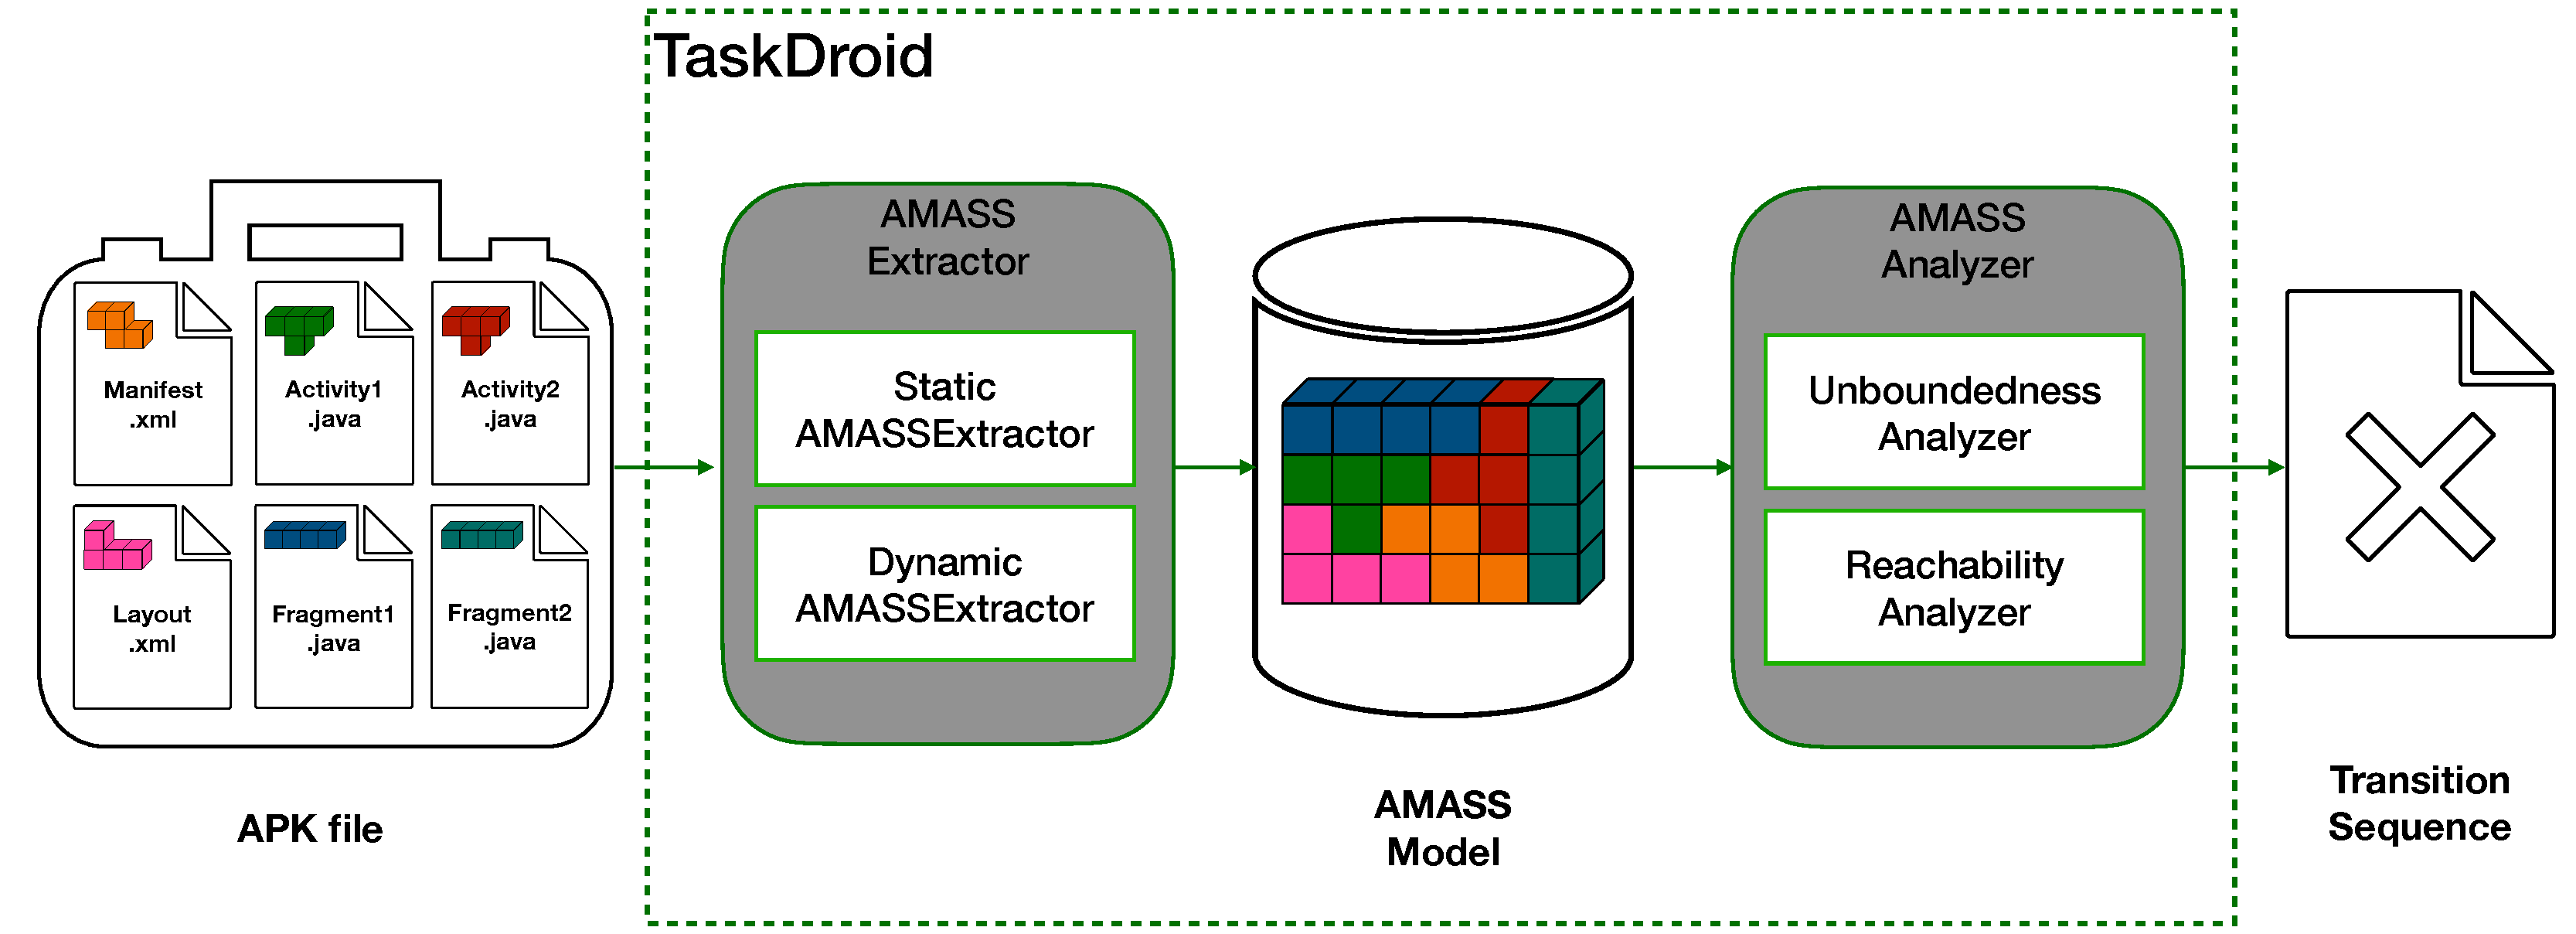
\includegraphics[scale=0.23]{taskdroid.pdf}
	\caption{Architecture of TaskDroid}
	\label{fig:taskdroid}
\end{figure}

%%%%%%%%%%%%%%%%%%%%%%%%%%%%%%%%%%%%%%%%%%%%%%%%%%%%%%%%%%%%%%%%%%%%%%

\subsection{Evaluation}\label{sec:bench}

We evaluate the efficiency and effectiveness of TaskDroid on 8,887 open source and commercial apps 
(cf.\ Section~\ref{sec:scal} and Section~\ref{sec:manual}). 
Moreover, we evaluate the impact of different model extractors on the detection of task/fragment container unboundedness problems of these apps (Section~\ref{sec:cmp}).  

The benchmark used for the evaluation consists of 8,887 Android apps collected from Androzoo\footnote{\url{https://androzoo.uni.lu/}} which include all the 3,867 open-source apps in the F-Droid repository,\footnote{\url{https://f-droid.org/}} as well as 5,020 commercial apps in the Google Play market. 
For Google Play, the apps are selected according to the popularity (number of downloads).  
Statistics of these apps can be found in Table~\ref{tab:stat}.
%
%The average/maximum size of F-Droid apps are 4.9MB/285.0MB respectively, while the average/maximum size of Google Play apps are 15.7MB/361.9MB respectively (see Table~\ref{tab:stat}). 

\begin{table}[htbp]   
\begin{center}   
\begin{tabular}{|c|c|c|c|}   
    \hline   \textbf{Source} & \textbf{\# apps}  &{\begin{tabular}{c} \textbf{Avg/Max. size} \\\textbf{of apps}\end{tabular}} & {\bf \begin{tabular}{c} \# extracted models \\
    (static/dynamic)\end{tabular} }  \\   
    \hline   F-Droid & 3,867  &4.9M/285.0M  & 3,471 (2,580/891)  \\ 
    \hline   Google Play & 5,020 &15.7M/361.9M  &4,612 (3,808/804)   \\  
\hline   
\end{tabular}  
\caption{Statistics of benchmarks \label{tab:stat}}   
\end{center}   
\end{table}

{\sf AMASSExtractor} extracts {\AMASS} models from the APK files as described in Section~\ref{sec:apk2amass}. 
\begin{itemize}
\item Out of the 3,867 F-Droid (resp.\ 5,020 Google Play) apps, static {\sf AMASSExtractor} extracts 2,580 (resp.\ 3,808) {\AMASS} models. Static {\sf AMASSExtractor} fails on 1,287 F-Droid (resp. 1,212 Google Play) apps, which is attributed to the fact that Soot fails to decompile the APK files or the source codes of the apps are obfuscated or encrypted. 

\item Out of the 2,580 models that are extracted from the F-Droid apps (called F-Droid models for short) by static {\sf AMASSExtractor} and 3,808 models that are extracted from the Google Play apps  (called Google-Play models for short) by static {\sf AMASSExtractor}, ICCBot$_{\AMASS}$ discovers that 311 F-Droid models and 501 Google-Play models respectively involve cross-app ICCs. 
Note that although ICCBot$_{\AMASS}$ discovers that these models involve cross-app ICCs, each of these models is extracted from \emph{one} APK file and the cross-app ICCs therein have not been dealt with yet. 
To remedy this, we tried to manually identify the APK files involved in these cross-app ICCs by searching for their package names. In the end, for 125 F-Droid apps and 211 Google-Play apps respectively, we provided the missing APK files involved in the cross-app ICCs of these apps and successfully constructed the {\AMASS} models for them where the cross-app ICCs are modeled. The average/maximum numbers and sizes of these missing apps involved in cross-app ICCs as well as the sizes of the extracted models are shown in Table~\ref{tab:missing-app}. Afterwards, these models can be analyzed in the same way as a model that is extracted from one APK file.
%
\item Moreover, among the 1,287 F-Droid (resp.\ 1,212 Google Play) apps that cannot be decompiled, dynamic {\sf AMASS} extracts 891 (resp.\ 804) {\AMASS} models. Dynamic {\sf AMASSExtractor} fails on 396 F-Droid (resp.\ 408 Google Play) apps, which is attributed to the fact that some apps cannot be launched, or crash after launching, or require user name and password to proceed after launching.  
\end{itemize}


\begin{table}
\begin{center}   
\begin{tabular}{|c | c | c |c |c |c |c |c |c |c |}   
    \hline    
    \multirow{2}{*}{\textbf{Source}}   & {\bf \begin{tabular}{c} \#apps containing \\ cross-app ICCs \end{tabular}} & {\begin{tabular}{c} \textbf{avg/max. numbers} \\ \textbf{of  missing apps}\end{tabular}}  & \begin{tabular}{c} \textbf{avg/max. sizes}  \\ {\bf of missing apps} \end{tabular}  & \multicolumn{3}{c|}{\textbf{avg/max. sizes of models}}  \\   
    \cline{5-7}    
    &&& & $|\act|$& $|\frag|$ & $|\Delta|$    \\ 
    \hline   
    F-Droid& 125 & 1.2/2 & 6.8M/103.2M& 6.2/38& 0.9/11 & 10.1/66   \\ 
    \hline   
    Google Play&804 & 1.5/2 &16.1M/153.3M& 7.9/19&1.1/20&14.5/97   \\  
\hline   
\end{tabular}   
\caption{Statistics of the missing apps involved in cross-app ICCs}
 \label{tab:missing-app} 
\end{center}   
\end{table}




\subsubsection{The efficiency of {\tool}}\label{sec:scal}
We investigate the efficiency and scalability of {\tool} by examining all 3,471 F-Droid and 4,612 Google Play apps for which AMASS models are extracted. For each app, static {\sf AMASSExtractor} extracts an {\AMASS} model from the APK file statically, where the timeout is set to 300 seconds. 
Moreover, for the apps where static {\sf AMASSExtractor} fails, dynamic {\sf AMASSExtractor} extracts an {\AMASS} model dynamically, where the time out is set to 600 seconds. 
The average/maximum sizes of the extracted models as well as the extraction time are shown in Table~\ref{tab:amass}--\ref{tab:amassdyn}.

%From Table~\ref{tab:amass},
It can be observed that, for the statically extracted models, the average/maximum size (number of transition rules, activities, fragments) of F-Droid apps is much smaller than that of Google Play apps. This is expected, since the  Google Play apps are considerably more complex than F-Droid open-source apps.
Moreover, the average time spent in the static model extraction of Google Play apps is over 5 times more than that of F-Droid apps.
Similar phenomenon happens for the dynamic model extraction, though the difference is slightly smaller. 
%than the static model extraction. 

%From Table~\ref{tab:amass}, 
Furthermore, static {\sf AMASSExtractor} can extract the {\sf AMASS} models for F-Droid apps in less than 1 minute and for Google Play apps in less than 4 mins, whereas %. On the other hand, from Table~\ref{tab:amassdyn}, 
dynamic {\sf AMASSExtractor} can extract the {\sf AMASS} models for F-Droid apps in around 5 mins and for Google Play apps in around 10 mins. The static model extraction is faster than the dynamic one, while the dynamic approach can deal with the apps that the static approach fails.

%Similarly, for the dynamic model extraction,  the average/maximum size (number of transition rules, activities, fragments) of F-Droid apps is much smaller than that of Google Play apps

%of transition rules ($|\Delta|$) is 7.9 (resp. 21.0) for F-Droid (resp. GooglePlay), the average number of activities ($|\act|$) is 4.9 (resp. 7.1) for F-Droid (resp. GooglePlay), the average number of fragments ($|\frag|$) is 0.5 (resp. 1.0) for F-Droid (resp. GooglePlay),
%the maximum number of transition rules ($|\Delta|$) for the AMASS models is 475 (resp. 1956) for F-Droid (resp. GooglePlay), the average number of activities ($|\act|$) is 70 (resp. 509) for F-Droid (resp. GooglePlay), the average number of fragments ($|\frag|$) is 16 (resp. 121) for F-Droid (resp. GooglePlay).
%The column Time shows the time used to extract the model. In general, the apps from Google Play are considerably more complex than F-Droid open-source apps, which incur about 6 times more processing time and 5 times more transition rules number.

\begin{table}[htbp]   
\begin{center}   
\begin{tabular}{|c |c |c |c |c |c |c |c|}   
    \hline    
    \multirow{2}{*}{\textbf{Source}}   &\multicolumn{3}{c|}{\textbf{Avg/Max. size of models}} & \multirow{2}{*}{\textbf{Avg. Time}} \\   
    \cline{2-4}    
    & $|\act|$& $|\frag|$ & $|\Delta|$ &   \\ 
    \hline   
    F-Droid & 4.9/70& 0.5/16 & 7.9/475 &  43.5s  \\ 
    \hline   
    Google Play & 7.1/509&1.0/121&21.0/1,956 & 234.6s  \\  
\hline   
\end{tabular}   
\caption{Static AMASSExtractor \label{tab:amass} }
\end{center}   
\begin{center}   
\begin{tabular}{|c|c|c|c|c|c|c|}   
    \hline  \multirow{2}{*}{\textbf{Source}}  &\multicolumn{2}{c|}{\textbf{Avg/Max. size of \AMASS}} & \multirow{2}{*}{\textbf{Avg. Time}} \\   
    \cline{2-3}   & $|\act|$& $|\Delta|$ &   \\ 
    \hline   F-Droid & 6.1/31&15.3/71 & 313.4s  \\  
    \hline   Google Play & 11.2/43&28.1/129 & 593.2s  \\  
\hline   
\end{tabular}   
\caption{Dynamic AMASSExtractor \label{tab:amassdyn} }
\end{center}   
\end{table}


%For each app in our bench marck (resp. 25 popular apps selected randomly from GooglePlay with more than 100,000 downloads), we build up an AMASS model from APK files via static extractor (resp. dynamic extractor), where the timeout is set to 300 seconds. The experimental results are shown in Table~\ref{tab:amass} (resp. Table~\ref{tab:amassdyn}),

%%%%%%%%%%%%%%%%%%%%%%%%%%%%%%%%%%%%%%%%%%%%%%%%%%%%%%%%%%%%%%%%%%%%%%%%%%%



%We investigate the effectiveness of our analysis approach in 
To detect %apps exhibiting the 
task/fragment container unboundedness vulnerabilities, the timeout is set to 30 seconds, the height $\hbar$ of tasks is set to 6 and $k$ (i.e., the number of interplaying tasks, cf.\ Section~\ref{sec:static}) is set to 2.

We first consider \revision{Android 13.0}. The results of task unboundedness (resp.\ fragment container unboundedness) 
are presented in Table~\ref{tab:taskbound}--\ref{tab:frgbound}. 
%Column \# Unbounded apps shows the number of detected apps which suffer from task unboundedness (resp. fragment stack unboundedness). Column \# Faulty cycles per app shows the number of witness cycles of each task unbounded (resp. fragment stack unbounded) app. Column Time shows the average time to perform the analysis. 
As one may see, {\tool} is highly efficient %fast 
in analyzing the {\AMASS} models, % against the task and fragment container unboundedness problems, 
which can be done 
in less than 0.1 seconds per app on average.
%
Moreover, {\tool} identifies 485 (14.0\%) F-Droid and 559 (12.1\%) GooglePlay models as ``task unbounded''.
On the other hand, %from Table~\ref{tab:frgbound}, 
{\tool} identifies 193 (5.6\%) F-Droid  and  293 (6.4\%) Google Play models as ``fragment container unbounded''. 
Finally, the number of witness cycles discovered for the unbounded models is around 3 per app on average.

\begin{table}[htbp]   
\begin{center}   
\begin{tabular}{|c|c|c|c|}   
    \hline   \textbf{Source}  &\begin{tabular}{c}\textbf{\#Unbounded}\\ \textbf{models}\end{tabular} & \begin{tabular}{c} \#\textbf{witness cycles} \\ \textbf{per model}\end{tabular} & \textbf{Time(s)} \\   
    \hline   F-Droid & 485/3,471 (14.0\%) & 3.3 &  0.05s  \\ 
    % \hline   F-Droid & Activity-based &413/3,471(11.9\%) & 3.1 &  0.05s  \\ 
    \hline   Google Play & 559/4,612 (12.1\%)&3.9 & 0.1s  \\  
    % \hline   Google Play & Activity-based &468/4,612(10.1\%)&3.4 & 0.1s  \\  
    %\hline   Google Play\# &9(36\%)&4.2 & 10.3s  \\  
\hline   
\end{tabular}   
\caption{Task Unboundedness \label{tab:taskbound} }
\end{center}   
\end{table}

\begin{table}[htbp]   
\begin{center}   
\begin{tabular}{|c|c|c|c|}   
    \hline   \textbf{Source} &\begin{tabular}{c}\textbf{\#Unbounded}\\ \textbf{models}\end{tabular} & \begin{tabular}{c} \#\textbf{witness cycles} \\ \textbf{per model}\end{tabular} & \textbf{Time(s)} \\   
    \hline   F-Droid & 193/2,580 (7.5\%) & 2.5 &  0.05   \\ 
    \hline   Google Play &293/3,808 (7.7\%)&3.0 & 0.1   \\  
\hline   
\end{tabular}   
\caption{Fragment Container Unboundedness \label{tab:frgbound} }
\end{center}   
\end{table}

We then consider Android 6.0--12.0 and compare the results for these versions with those for \revision{Android 13.0}. As shown in Figure~\ref{fig:cmp-and}, the numbers of task unbounded F-Droid (resp.\ Google Play) apps are slightly different for different versions, while the numbers of fragment container unbounded F-Droid (resp.\ Google Play) apps are the same for different versions. This phenomenon is explained by that the semantics of $\AOAMASS$ is slightly different across Android versions, while the semantics of $\FOAMASS$ is the same for all these versions. To have a closer look, we can see that the numbers of task unbounded F-Droid (resp.\ Google Play) apps for Android 7.0, Android 8.0--10.0, and \revision{Android 11.0--13.0} are close to each other, and are slightly away from that of Android 6.0. This is explained by that Android 6.0 uses a different task allocation mechanism from the others. 


%%%%%%%%%%%%%%%%%%%%%%%%%%
%%%%%%%%%%%%%%%%%%%%%%%%%%
\hide{
\revision{Although our algorithm is primarily designed for analyzing individual apps, it can also handle the analysis of interactions between multiple apps. In such cases, we construct an {\AMASS} model that includes the activities, fragments, transition rules, and other components of the relevant apps. The main activity of the analyzed app is set as the main activity $A_0$ of the model. In the sequel, these apps can be treated as one app for further analysis. There are $311$ (resp. $501$) models comprising the cross-app ICC out of $3,471$ (resp. $4,612$) extracted models in F-Droid (resp. Google Play).  As illustrated in Figure~\ref{fig:cross-app}, when considering cross-app ICC, we obtain the same results in detecting fragment container unboundedness vulnerabilities, as app-switching does not add new activities to the analyzed app.  Additionally, there is a slight increase in the detection of task unbounded apps. 
This is primarily due to the fact that over 91\% of the models (739 out of 812) with cross-app ICC exhibit the behavior of remaining in the background after switching to another app, which is similar to the situation when cross-app ICC is not considered.}
}
%%%%%%%%%%%%%%%%%%%%%%%%%%
%%%%%%%%%%%%%%%%%%%%%%%%%%

% the number of the fragment container unbounded models detected is the same under Android 6.0-Android 12.0, the number of the task unbounded models detected under Android 6.0, Android 8.0-Android 10.0 is more than the one under Android 12.0, while the number of the task unbounded models detected under Android 7.0 is less than the one under Android 12.0.

%In summary, for 3,471 F-Droid (resp. 4,612 Google Play)  apps, TaskDroid can extract the {\AMASS} models from APK files and finish the unboundedness analysis in around 5 minutes (resp. 10 minutes) per app, where the vast majority of the time is spent in the extraction of an {\AMASS} model and the unboundedness analysis of the model is pretty fast. 

%It can be observed that, for apps from F-Droid, when we adopt a simple $\AMASS$ model, 108 (out of 2,580) apps are found to have UBA abnormality, but when a full $\AMASS$ model is used, 251 apps are detected, which gives an increase of 132\%. The same thing is observed for the apps from Google Play. The increases on the number of abnormal transition rules are even higher. This highlights the importance and benefit of adopting a full-fledged semantics for the multitasking mechanism, including features such as fragments. We remark that a full  $\AMASS$ model allows to capture  more cases of UBA, for instance, the case (1) with $\ntkflag$ and the case (2) where fragments are involved. 
%In terms of the efficiency, the average time is 0.2 second for relatively small apps from F-Droid and 1.1 second for larger apps from Google Play. 





% \begin{figure}%[h]
% \centering
% 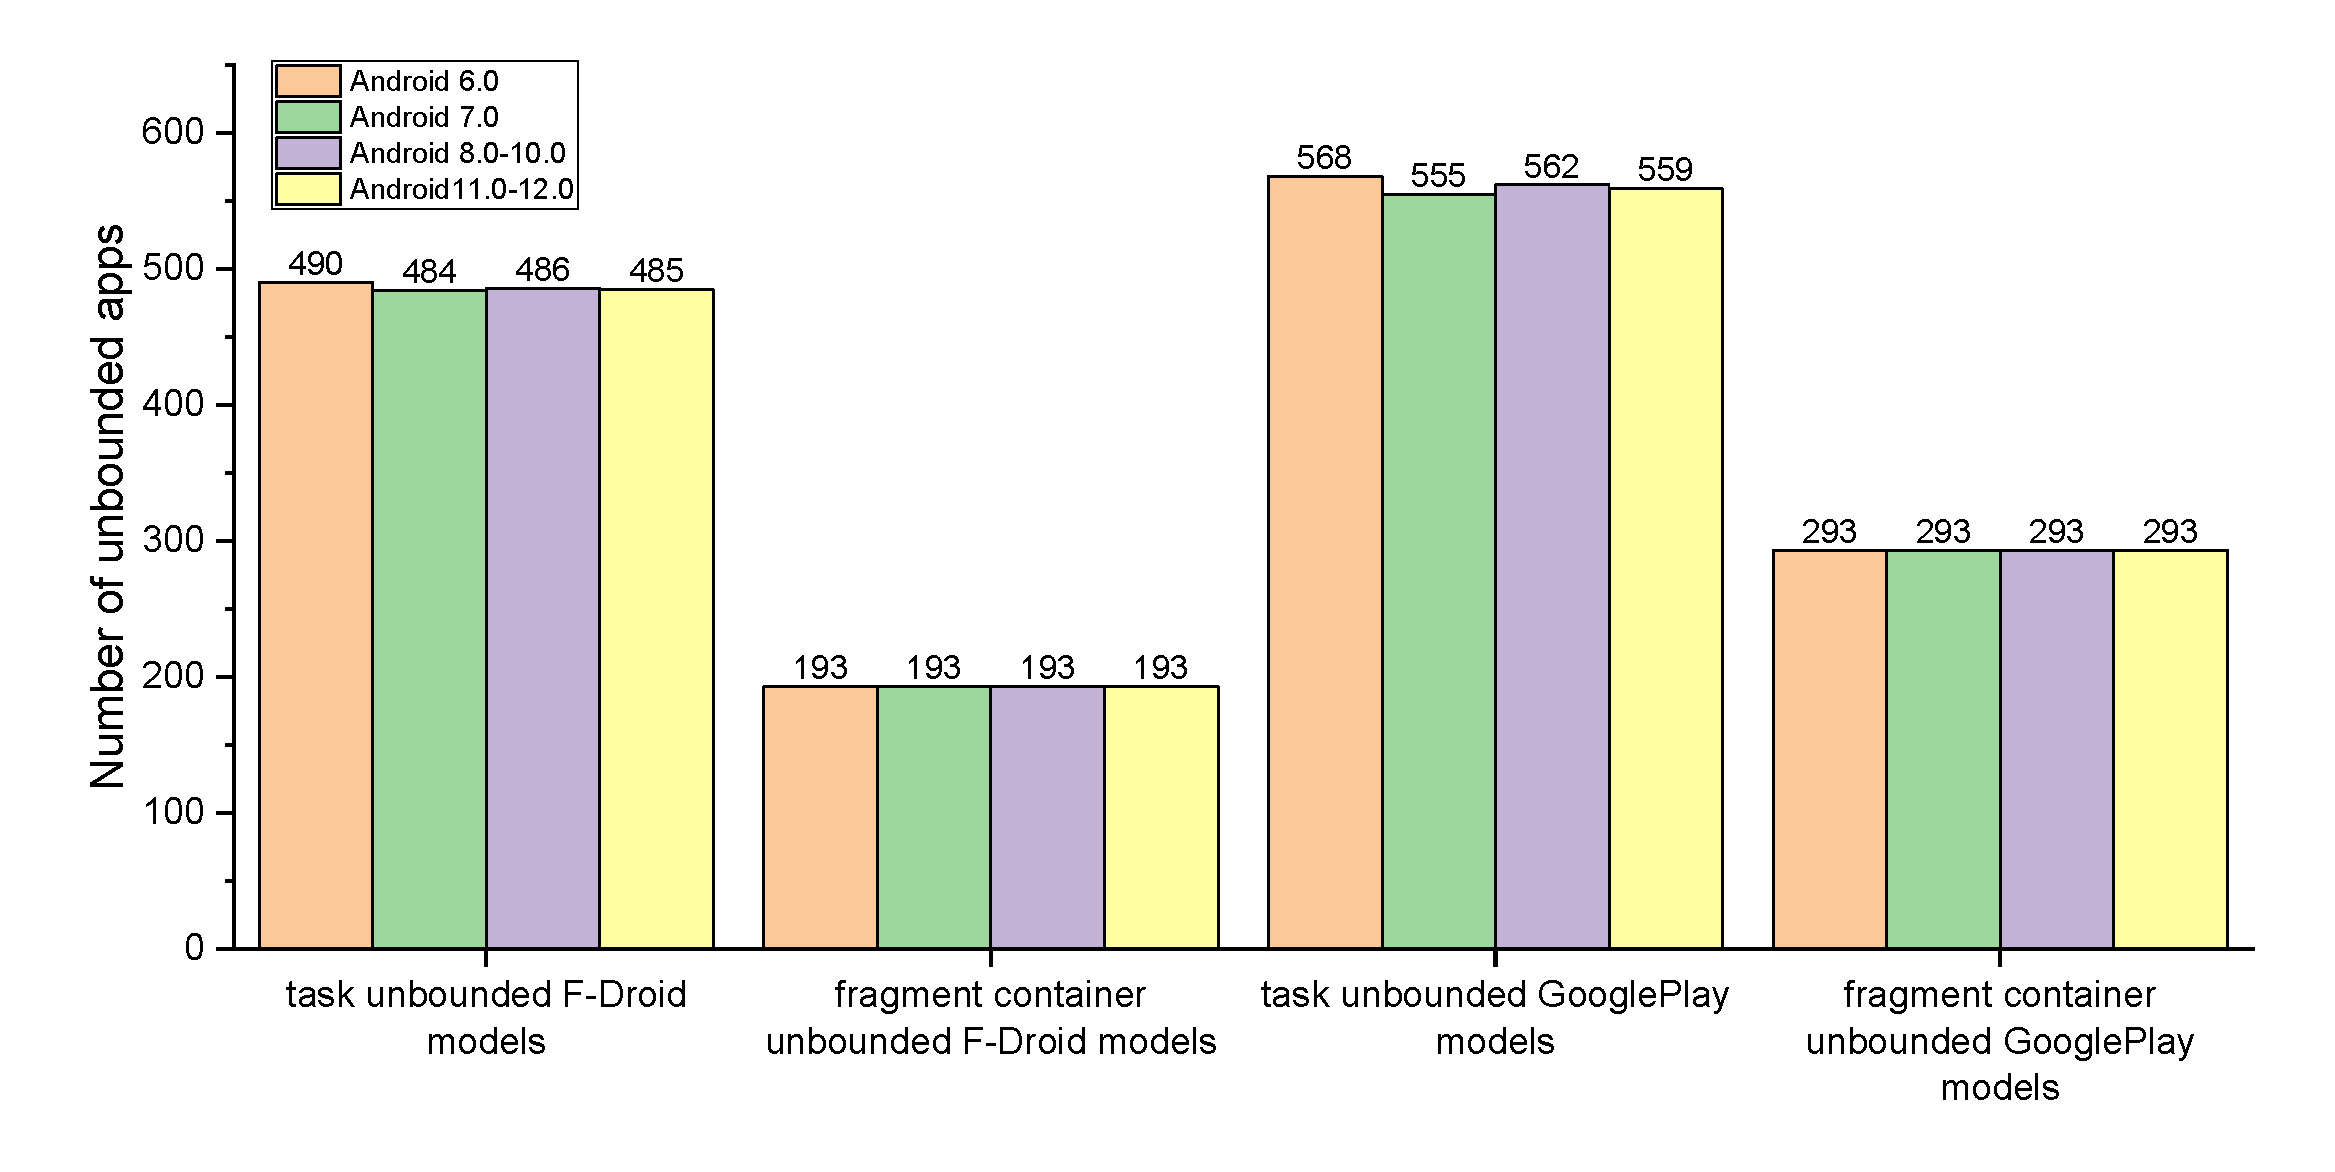
\includegraphics[scale=0.35]{android-version.pdf}
% \caption{Unboundedness under different Android versions}
% \label{fig:ubd-android}
% \end{figure}
\begin{figure}[htbp]
	\begin{minipage}[t]{0.49\linewidth}
		\centering
		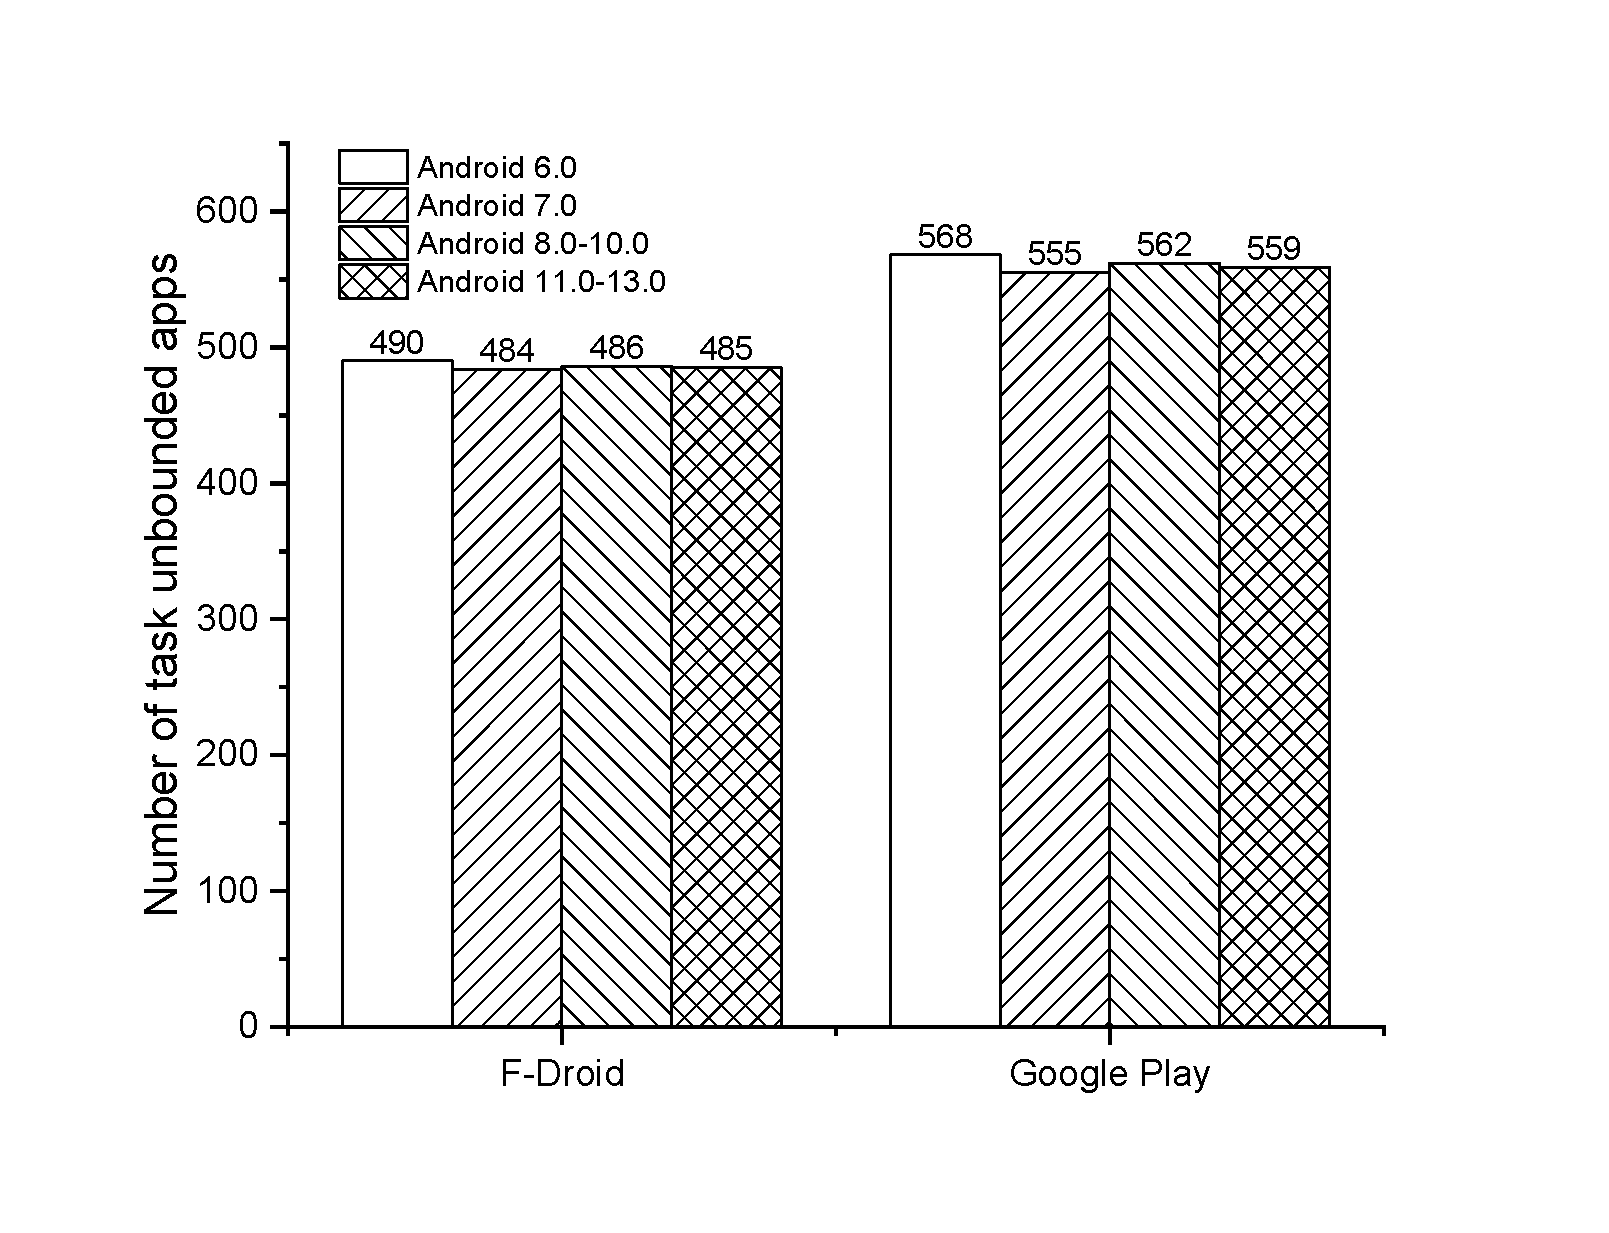
\includegraphics[width=3.2in]{cmp-and-task.pdf}
	\end{minipage}
	\begin{minipage}[t]{0.49\linewidth}
		\centering
		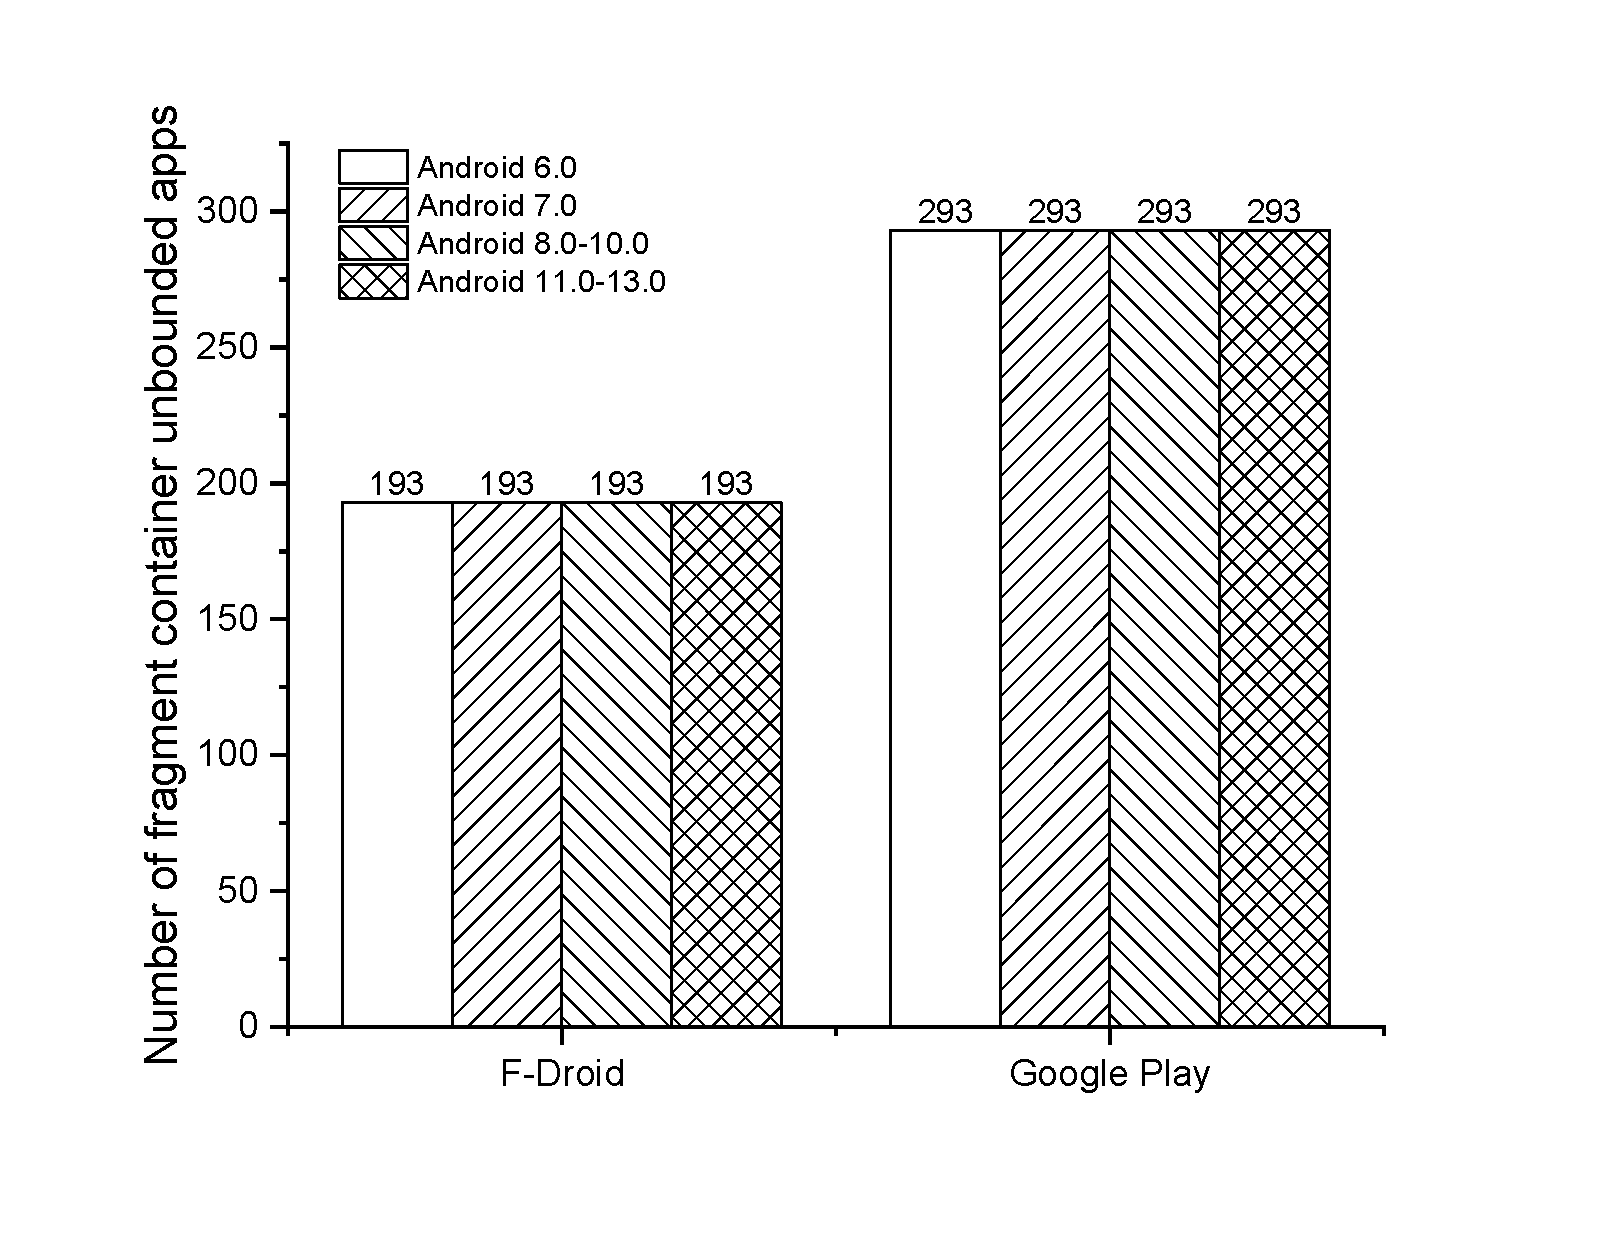
\includegraphics[width=3.2in]{cmp-and-frag.pdf}
	\end{minipage}
	\caption{\revision{Comparison of the results for different Android versions}}
	\label{fig:cmp-and}
\end{figure}

\hide{
\begin{figure}
	\begin{minipage}[t]{0.49\linewidth}
		\centering
		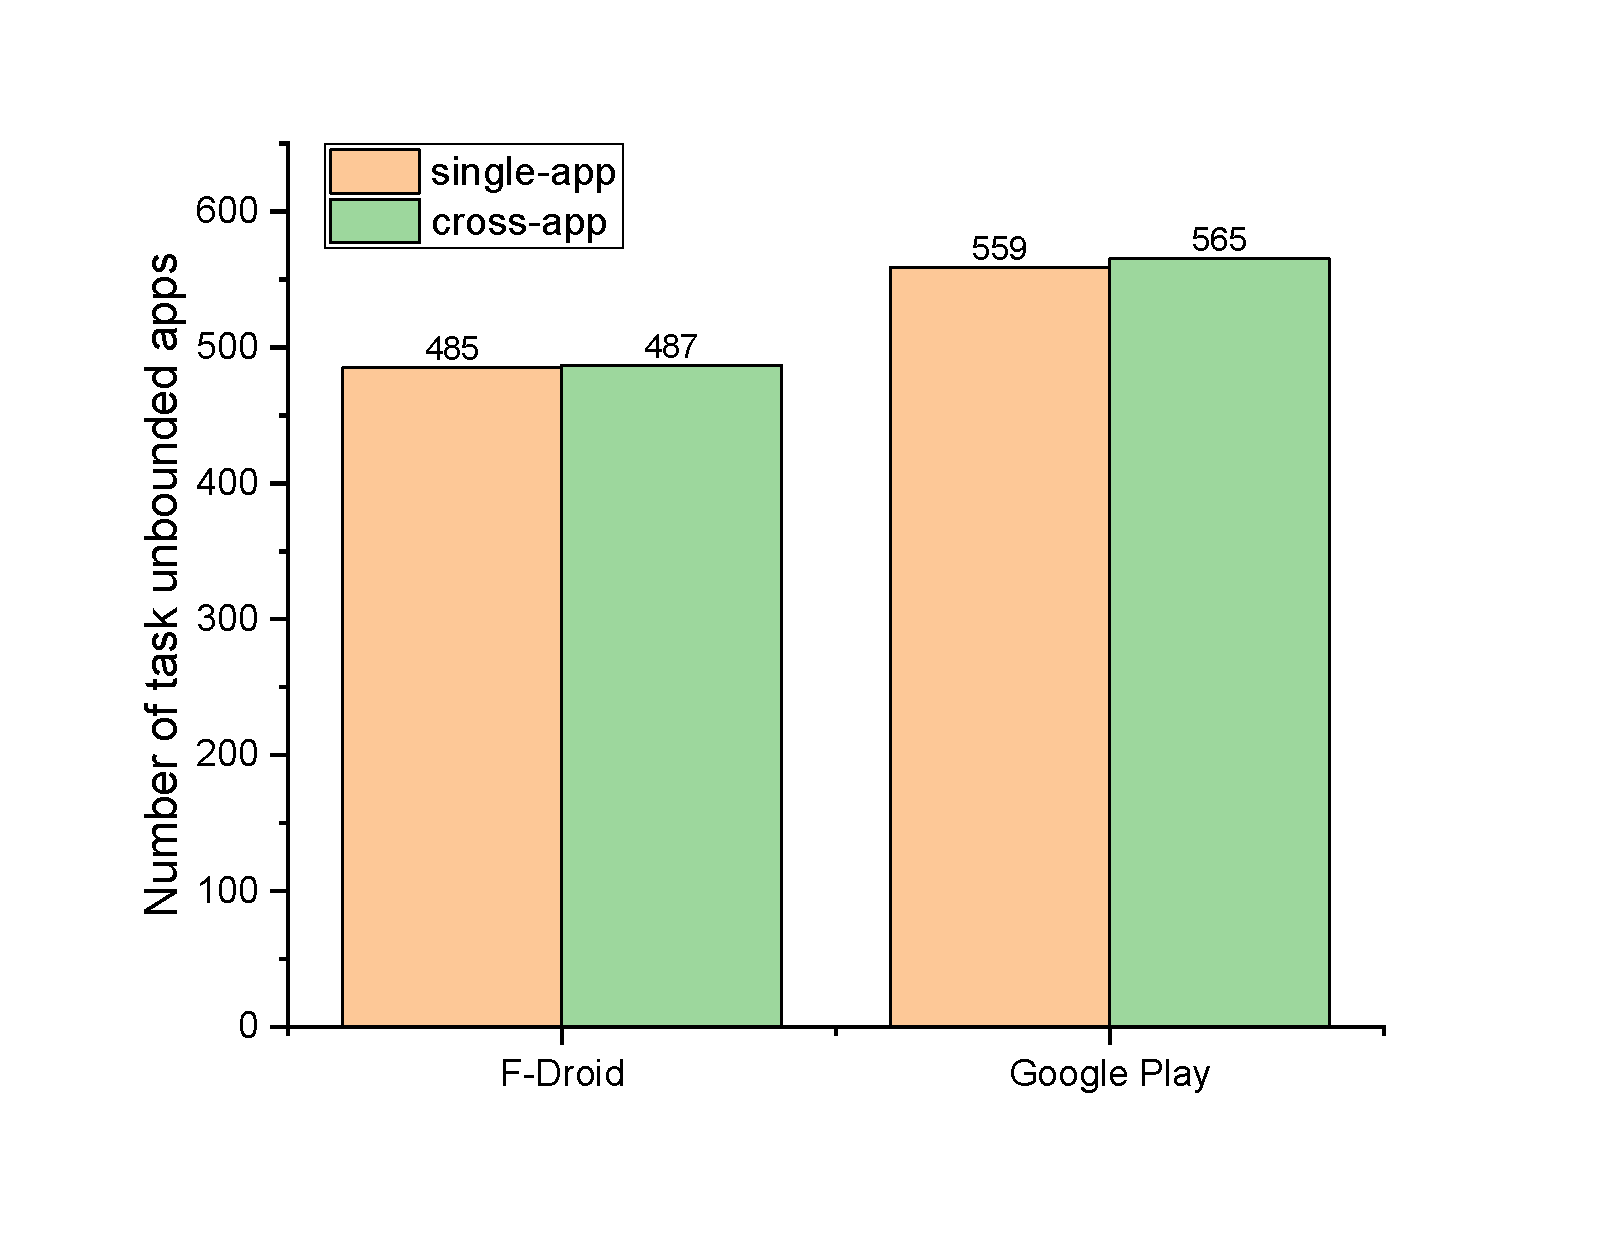
\includegraphics[width=3.2in]{task_unb_cross.pdf}
	\end{minipage}
	\begin{minipage}[t]{0.49\linewidth}
		\centering
		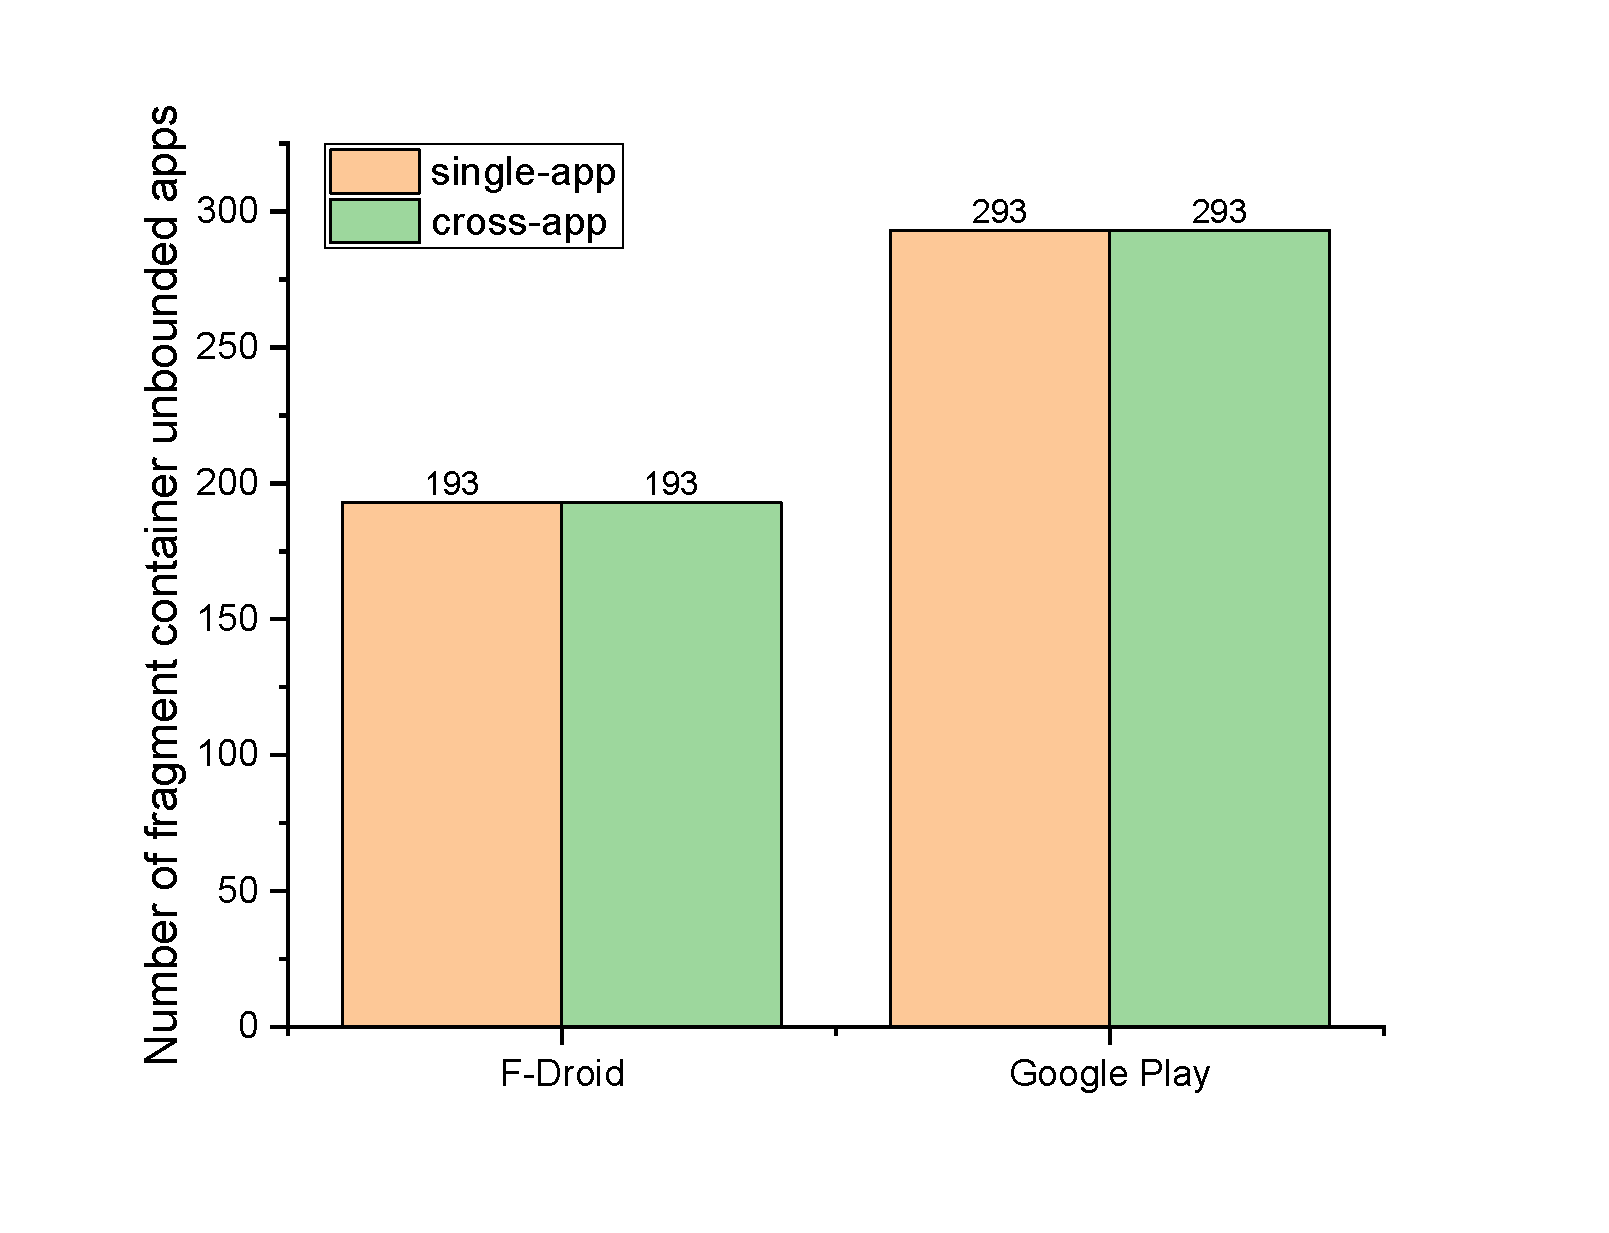
\includegraphics[width=3.2in]{frag_unb_cross.pdf}
	\end{minipage}
	\caption{Unboundedness when (resp. not) considering cross-app ICC}
	\label{fig:cross-app}
\end{figure}
}



\subsubsection{The effectiveness of \tool} \label{sec:manual}
 %
We investigate whether {\tool} can accurately detect task/fragment container unboundedness vulnerabilities, and the abnormal behavior caused by these vulnerabilities in Android mobile device.  
To this end, we randomly select 50 apps from those that are identified as ``task unbounded'' and  ``fragment container unbounded'' by {\tool} respectively, in each case 25 are from F-Droid and 25 are from GooglePlay.
The information of these apps can be found in  Appendix~\ref{app:table}, Table~\ref{tab:t-unb-rand-fd}~--~\ref{tab:fc-unb-rand-gg}. 


%\begin{table*}[t]
%\begin{center}   
%\caption{Statistics of 50 randomly selected ``task-unbounded'' apps \label{tab:t-unb-rand} }
%\begin{tabular}{|c|c|c|c|c|c|}   
%    \hline   \textbf{Source} &\textbf{Package name} &\textbf{$|\act|$} & \textbf{$|\frag|$} & \textbf{$|\Delta|$} & \textbf{Size(MB)} \\   
%%
%    \hline   F-Droid  & org.gnucash.android & 10 & 2& 32 & 2.71  \\ 
%    \hline   F-Droid  & systems.byteswap.aiproute & 3& 0& 3& 1.08  \\ 
%    \hline   F-Droid  & max.music\_cyclon & 2& 0& 2& 1.81 \\ 
%    \hline   F-Droid  & com.matburt.mobileorg & 8& 0& 9& 1.36 \\ 
%    \hline   F-Droid  & org.npr.android.news & 5& 0& 8& 0.92 \\ 
%    \hline   F-Droid  & com.commonsware.android.arXiv & 8& 0& 12& 0.52 \\ 
%    \hline   F-Droid  & net.mabako.steamgifts & 6& 1& 24& 2.66 \\ 
%    \hline   F-Droid  & com.app.Zensuren & 17& 0& 22& 0.17 \\ 
%    \hline   F-Droid  & uk.co.busydoingnothing.prevo & 4& 0& 5& 11.79 \\ 
%    \hline   F-Droid  & de.drhoffmannsoftware.calcvac & 14& 0& 24& 0.9 \\ 
%    \hline   F-Droid  & org.sasehash.burgerwp & 2& 0& 3& 1.76 \\ 
%    \hline   F-Droid  & com.mikifus.padland & 6& 1& 18& 1.07  \\ 
%    \hline   F-Droid  & org.evilsoft.pathfinder.reference & 5& 0& 8& 22.02  \\ 
%    \hline   F-Droid  & com.android.keepass & 4& 0& 6& 1.65  \\ 
%    \hline   F-Droid  & de.bloosberg.basti.childresuscalc & 2& 0& 2& 1.41  \\ 
%    \hline   F-Droid  & com.samebits.beacon.locator & 2& 0& 2& 1.98  \\ 
%    \hline   F-Droid  & ohm.quickdice & 9& 0& 14& 1.41  \\ 
%    \hline   F-Droid  & org.saiditnet.redreader & 11& 1& 51& 4.99  \\ 
%    \hline   F-Droid  & com.gianlu.aria2app & 13& 0& 31& 21.11  \\ 
%    \hline   F-Droid  & net.artificialworlds.rabbitescape & 3& 0& 3& 18.81  \\ 
%    \hline   F-Droid  & com.sam.hex & 10& 0& 23& 0.76  \\ 
%    \hline   F-Droid  & com.kaliturin.blacklist & 2& 0& 2& 2.06  \\ 
%    \hline   F-Droid  & de.schildbach.oeffi & 10& 0& 35& 1.79  \\ 
%    \hline   F-Droid  & com.aurora.store & 22& 0& 56& 5.47  \\ 
%    \hline   F-Droid  & com.adrienpoupa.attestationcoronavirus & 2& 0& 2& 3.58  \\ 
%%    \hline   \multicolumn{2}{|c|}{\textbf{Average}} & 7.2& 0.2& 15.9& 4.6  \\ 
%%
%    \hline   GooglePlay  & com.abdulqawi.ali.mosabqa & 8& 0& 25& 2.84  \\ 
%    \hline   GooglePlay  & com.music.star.player & 3& 3& 25& 2.38  \\ 
%    \hline   GooglePlay  & com.drclabs.android.wootchecker & 11& 0& 18& 0.84  \\ 
%    \hline   GooglePlay  & com.hotels.hotelsmecca & 6& 1& 16& 16.43  \\ 
%    \hline   GooglePlay  & com.airg.hookt & 6& 0& 12& 10.59  \\ 
%    \hline   GooglePlay  & com.holidu.holidu & 2& 0& 2& 4.04  \\ 
%    \hline   GooglePlay  & com.appkey.english3000freekata & 28& 0& 97& 1.06  \\ 
%    \hline   GooglePlay  & socials.com.application & 34& 0& 122& 3.75  \\ 
%    \hline   GooglePlay  & www.genting.rwgenting & 3& 0& 5& 12.78  \\ 
%    \hline   GooglePlay  & com.goldenhammer.beisboldominicana & 3& 1& 10& 4.58  \\ 
%    \hline   GooglePlay  & com.travolution.seoultravelpass & 5& 0& 10& 4.58  \\ 
%    \hline   GooglePlay  & com.ic.myMoneyTracker & 25& 0& 60& 3.39  \\ 
%    \hline   GooglePlay  & tekcarem.gebeliktakibi & 59& 0& 255& 3.15  \\ 
%    \hline   GooglePlay  & de.fckoeln.app & 22& 0& 45& 40.77  \\ 
%    \hline   GooglePlay  & de.twokit.castbrowser & 5& 0& 8& 3.79  \\ 
%    \hline   GooglePlay  & com.TWTD.FLIXMOVIE & 6& 0& 10& 7.73  \\ 
%    \hline   GooglePlay  & com.emeint.android.mwallet.tub & 10& 0& 95& 59.02  \\ 
%    \hline   GooglePlay  & com.ctt.celltrak2 & 22& 0& 80& 11.31  \\ 
%    \hline   GooglePlay  & biz.mobinex.android.apps.cep\_sifrematik & 11& 0& 34& 3.54  \\ 
%    \hline   GooglePlay  & com.linesmarts.linesmartsfree & 4& 0& 4& 28.47  \\ 
%    \hline   GooglePlay  & com.nhiApp.v1 & 8& 9& 107& 26.6  \\ 
%    \hline   GooglePlay  & com.alfarooqislamicresearchcenter & 34& 0& 78& 13.83  \\ 
%    \hline   GooglePlay  & com.objectremover.touchretouch & 14& 0& 19& 11.28  \\ 
%    \hline   GooglePlay  & com.vwfs.phototan & 3& 0& 5& 27.23  \\ 
%    \hline   GooglePlay  & com.sg.apphelperstore & 5& 0& 6& 6.56  \\ 
%%    \hline   \multicolumn{2}{|c|}{\textbf{Average}} & 13.5& 0.6& 45.9& 12.4  \\ 
%
%    
%\hline   
%\end{tabular}   
%\end{center}   
%\end{table*}
%
%\begin{table*}[t]
%\begin{center}   
%\caption{Statistics of 50 randomly selected ``fragment-container unbounded'' apps \label{tab:fc-unb-rand} }
%\begin{tabular}{|c|c|c|c|c|c|}   
%    \hline   \textbf{Source} &\textbf{Package name} &\textbf{$|\act|$} & \textbf{$|\frag|$} & \textbf{$|\Delta|$} & \textbf{Size(MB)} \\   
%%
%    \hline   F-Droid & org.ligi.fahrplan & 6& 5& 46& 1.83  \\ 
%    \hline   F-Droid  & io.gitlab.allenb1.todolist & 6& 3& 11& 1.05  \\ 
%    \hline   F-Droid  & naman14.timber & 5& 3& 15& 5.8  \\ 
%    \hline   F-Droid  & me.anon.grow & 4& 3& 30& 6.46  \\ 
%    \hline   F-Droid  & com.wikijourney.wikijourney & 1& 2& 7& 4.27  \\ 
%    \hline   F-Droid  & com.mattallen.loaned & 3& 1& 5& 1.01  \\ 
%    \hline   F-Droid  & com.ymber.eleven & 1& 2& 15& 10.38  \\ 
%    \hline   F-Droid  & com.syncedsynapse.kore2 &2& 1& 5& 2.22  \\ 
%    \hline   F-Droid  & net.momodalo.app.vimtouch & 5& 1& 9& 3.44  \\ 
%    \hline   F-Droid  & com.csipsimple & 12& 2& 22& 11.56  \\ 
%    \hline   F-Droid  & ch.corten.aha.worldclock & 4& 3& 13& 1.4  \\ 
%    \hline   F-Droid  & org.wikimedia.commons.wikimedia & 3& 6& 44& 15.0  \\ 
%    \hline   F-Droid  & com.llamacorp.equate & 1& 1& 3& 0.39  \\ 
%    \hline   F-Droid  & koeln.mop.elpeefpe & 4& 2& 11& 1.59  \\ 
%    \hline   F-Droid  & fr.kwiatkowski.ApkTrack & 1& 2& 13& 2.32  \\ 
%    \hline   F-Droid  & eu.siacs.conversations.legacy & 17& 2& 88& 11.12  \\ 
%    \hline   F-Droid  & com.artifex.mupdfdemo & 4& 2& 5& 25.68  \\ 
%    \hline   F-Droid  & org.osmdroid  & 15& 3& 28& 4.62  \\ 
%    \hline   F-Droid  & com.haha01haha01.harail & 4& 1& 6& 0.69   \\ 
%    \hline   F-Droid  & com.owncloud.android & 11& 4& 40& 3.8  \\ 
%    \hline   F-Droid  & org.cipherdyne.fwknop2 & 5& 2& 12& 2.63  \\ 
%    \hline   F-Droid  & edu.cmu.cylab.starslinger.demo & 4& 1& 8& 1.21  \\ 
%    \hline   F-Droid & com.commonslab.commonslab & 4& 6& 45& 14.72  \\ 
%    \hline   F-Droid  & hans.b.skewy1\_0 & 1& 6& 19& 6.45  \\ 
%    \hline   F-Droid  & com.twobuntu.twobuntu & 4& 3& 12& 0.75  \\ 
%%    \hline   \multicolumn{3}{|c|}{\textbf{Average}} & 5.1& 2.7& 20.5& 5.6  \\ 
%%
%    \hline   GooglePlay  & com.schoola2zlive & 11& 1& 40& 4.77  \\ 
%    \hline   GooglePlay  & com.endless.smoothierecipes & 3& 9& 110& 7.57  \\ 
%    \hline   GooglePlay  & com.traderumors & 5& 6& 28& 5.53  \\ 
%    \hline   GooglePlay & com.rakuten.room & 20& 19& 87& 20.1  \\ 
%    \hline   GooglePlay  & com.hotels.hotelsmecca & 6& 1& 16& 16.43  \\ 
%    \hline   GooglePlay  & br.com.prevapp03 & 34& 1& 80& 5.15  \\ 
%    \hline   GooglePlay  & com.star.mobile.video & 21& 1& 55& 7.98  \\ 
%    \hline   GooglePlay  & fr.elol.yams & 4& 6& 93& 8.75  \\ 
%    \hline   GooglePlay  & music.symphony.com.materialmusicv2 & 7& 3& 14& 3.39  \\ 
%    \hline   GooglePlay  & ru.sports.rfpl & 6& 1& 9& 8.33  \\ 
%    \hline   GooglePlay  & com.discsoft.daemonsync & 7& 1& 10& 10.06  \\ 
%    \hline   GooglePlay  & com.accuvally.android.accupass & 8& 1& 21& 11.62  \\ 
%    \hline   GooglePlay  & com.directv.navigator & 10& 7& 68& 41.66  \\ 
%    \hline   GooglePlay  & com.ldf.gulli.view & 13& 8& 49& 15.62  \\ 
%    \hline   GooglePlay  & kvp.jjy.MispAndroid320 & 14& 6& 51& 31.34  \\ 
%    \hline   GooglePlay  & de.wirfahrlehrer.easytheory & 3& 12& 144& 3.6  \\ 
%    \hline   GooglePlay  & com.mmb.mamitalk & 5& 4& 22& 8.19  \\ 
%    \hline   GooglePlay  & ch.swissdevelopment.android & 3& 1& 8& 20.55  \\ 
%    \hline   GooglePlay  & tw.com.iobear.medicalcalculator & 1& 1& 3& 2.49  \\ 
%    \hline   GooglePlay  & com.gn.apkmanager & 2& 1& 4& 2.92  \\ 
%    \hline   GooglePlay  & com.piradevrcostagen.strobo & 2& 1& 4& 2.48  \\ 
%    \hline   GooglePlay  & com.gqueues.android.app & 13& 3& 34& 4.68  \\ 
%    \hline   GooglePlay  & com.reverb.app & 14& 9& 96& 13.82  \\ 
%    \hline   GooglePlay  & com.xnview.hypocam & 4& 8& 36& 26.23  \\ 
%    \hline   GooglePlay  & de.stefanpledl.localcast & 1& 16& 95& 13.94  \\ 
% %   \hline   \multicolumn{3}{|c|}{\textbf{Average}} & 8.7& 5.1& 47.1& 11.9  \\   
%\hline   
%\end{tabular}   
%\end{center}   
%\end{table*}

We manually check on a virtual machine (4-core CPU, 2G RAM with \revision{Android 13.0}) whether these 100 apps are indeed task/fragment-container unbounded by verifying whether the witness cycles reported by {\tool} are executable. \revision{To ensure the reliability of the manual checking, we %apply the cross verification method and 
ask 4 individuals to complete the manual checking and each of them checks all the 100 apps. The results are cross checked, and summarized in Table~\ref{tab:man-taskbound}}.

%We use cross-verification method involving 4 individuals to check manually

\begin{table}[htbp]   
	\begin{center}   
		\begin{tabular}{|c|c|c|c|}   
			\hline   \textbf{Source} & \textbf{unbound. vulnerability} &{\begin{tabular}{c} \textbf{\#apps}\end{tabular}} &{\begin{tabular}{c} \textbf{\#confirmed} \\\textbf{apps}\end{tabular}}   \\   
			\hline
			\hline   F-Droid & task & 25 & 17 (68\%)   \\ 
			\hline   GooglePlay & task & 25 & 16 (64\%)   \\ 
			\hline   F-Droid & {\begin{tabular}{c} fragment \\ container \end{tabular}} & 25 & 16 (64\%)   \\ 
			\hline   GooglePlay & { \begin{tabular}{c} fragment \\ container \end{tabular}} & 25 & 16 (64\%)  \\ 
			\hline 
			\hline  \begin{tabular}{c} F-Droid or\\ GooglePlay \end{tabular} & task & 50 & 33 (66\%) \\    
			\hline  \begin{tabular}{c} F-Droid or \\ GooglePlay \end{tabular} &\begin{tabular}{c} fragment \\ container \end{tabular} & 50 & 32 (64\%) \\    
			\hline
			\begin{tabular}{c}F-Droid or\\ GooglePlay\end{tabular} &
			\begin{tabular}{c} task or \\ fragment \\ container \end{tabular}& 100 & 65 (65\%) \\
			%\hline   Google Play &445(11.8\%)&1,794  \\  
			\hline   
		\end{tabular}   
		\caption{Manual confirmation of the effectiveness of {\tool} \label{tab:man-taskbound}}
	\end{center}   
\end{table}

Out of the 25 apps from F-Droid (resp.\ GooglePlay), 17 (resp.\ 16) apps are confirmed to be task unbounded, occupying 68\% (resp.\ 64\%) of the randomly chosen apps;  
16 (resp.\ 16) apps are confirmed to be fragment-container unbounded, occupying 64\% (resp. 64\%) of the randomly chosen F-Droid (resp.\ GooglePlay) apps. %Therefore, according to the results, the 
These give an overall accuracy of 65\%. 
%, since 65 out of 100 apps are confirmed to be task/fragment-container unbounded. 
For the rest 35 apps, we could not confirm the analysis result, because: %unboundedness, attributed to the following reasons:  
9 apps require login, 9 apps crash immediately after launching, and 17 apps %are not precise so that 
could not execute the witness cycles (we suspect that the witness cycles in these {\AMASS} models 
are spurious). %can not be executed. 
%We also observe that the overall accuracy of task unboundedness (68\%) is better than that of fragment-container unboundedness (58\%). This fact is potentially attributed to \zhilin{xxx}.

%We manually examine whether these 100 apps are task/fragment stack unbounded, and then analyze and report the experimental results in Section~\ref{sec:manual}.
%%%%%%%%%%%%%%%%%%%%%%%%%%%%%%%%%%
%%%%%%%%%%%%%%%%%%%%%%%%%%%%%%%%%%
%\hide{
	%For task boundedness analysis (resp. fragment stack boundedness analysis), we respectivly select 25 task unbounded (resp. fragment stack unbounded) apps from F-Droid and 25 task unbounded (resp. fragment stack unbounded) apps from GooglePlay randomly, 
	%we manually inspect the unbounded problems for these applications to evaluate how many problems correspond to real exploiteble problems.
	%Moreover, according to the reachability path for unboundedness which is generated from a witness cycle, for each activity $A$ (resp. fragment $F$), we locate the UI widget corresponding to $A$ (resp. $F$) by 
	%using ADB tool to check whether the top activity (resp. fragment) corresponding to the transition rule's target when clicking some UI widget.
	%As shown in Figure~\ref{tab:man-taskbound}, for task boundedness analysis we confirm 18 (resp. 16) applications could be suffered task unbounded problem, this represents a 72\% (resp. 64\%) true positive rate, for fragment stack boundedness analysis we confirm 15 (resp. 14) applications could be suffered fragment stack unbounded problem, this represents a 60\% (resp. 56\%) true positive rate.
	%Moreover, we successfully simulated 63 apps out of 100 apps from F-Droid and GooglePlay, for the other 37 apps, we were unable to  simulate the witness cycles, due to the following reasons:   login is required (10 apps), apps crash immediately after launching (9 apps), AMASS models are imprecise (18 apps) so the potential threat returned by TaskDroid may be spurious.
	%The overall accuracy of fragment stack boundedness analysis is lower than task boundedness analysis, since we omit the remove action in the fragment transaction.
	%More details about the apps are presented in Section~\ref{sec:threat}.
	%}
%%%%%%%%%%%%%%%%%%%%%%%%%%%%%%%%%%
%%%%%%%%%%%%%%%%%%%%%%%%%%%%%%%%%%


 
Furthermore, on the same virtual machine, for each app that is confirmed to be ``task unbounded'' or ``fragment-container unbounded'', we use UIAutomator to execute the click-event sequence generated when simulating the witness cycle for many times until some abnormal behavior appears. 
During the execution, we use ADB to calculate the number of repetitions of the witness cycle as well as record the type of abnormal behavior of the virtual device. The results of the experiments are presented in Table~\ref{tab:threat-fd-task}--\ref{tab:threat-gg-f}. 
%For 
%Out of 25 task unbounded F-Droid (resp.\ GooglePlay) apps, the witness cycles synthesized by TaskDroid can be successfully simulated in 18 (resp.\ 16) apps. 
%
\begin{itemize}
	\item Among the 18 (resp. 16) F-Droid (resp.\ GooglePlay) apps that are confirmed to be task unbounded, after hundreds of repetitions of the witness cycle, 10 (resp.\ 11) apps end up with rebooting of device, 6 (resp.\ 4) apps end up with app crash, and 2 (resp.\ 1) apps end up with restarting of app.
	%
	\item Among the 15 (resp. 14) F-Droid (resp. GooglePlay) apps that are confirmed to be fragment-container unbounded, after thousands of repetitions of the witness cycle, 2 (resp.\ 5) apps end up with rebooting of device, 10 (resp.\ 8) apps end up with app crash, and 3 (resp.\ 1) apps end up with restarting of app.
	%
\end{itemize}


\begin{table}[htbp]
	\begin{center}   
%		\begin{subtable}{10cm}	
		\begin{tabular}{|c|c|c|}   
			\hline   
			\textbf{Package name} & \shortstack{\#repetitions of \\ the witness cycle} & \textbf{Abnormal behavior} \\   
			\hline
			\hline   
			 org.gnucash.android & 215 & reboot  \\ 
			\hline   
			 systems.byteswap.aiproute & 203 &reboot  \\ 
			\hline   
			  max.music\_cyclon & 97  &reboot \\ 
			\hline   
			com.matburt.mobileorg & 204  &reboot \\ 
			\hline    org.npr.android.news & 192  &reboot \\ 
			\hline    com.commonsware.android.arXiv & 125  &reboot \\ 
			\hline    net.mabako.steamgifts & 103  &reboot \\ 
			\hline     com.app.Zensuren & 114  &reboot \\ 
			\hline   uk.co.busydoingnothing.prevo & 122  &reboot \\ 
			\hline    de.drhoffmannsoftware.calcvac & 208  &reboot \\ 
			\hline     org.sasehash.burgerwp & 240  &app crash \\ 
			\hline    com.mikifus.padland & 59 &app crash  \\ 
			\hline    org.evilsoft.pathfinder.reference & 179 &app crash  \\ 
			\hline     com.android.keepass & 150 & app crash  \\ 
			\hline    de.bloosberg.basti.childresuscalc & 288 & app crash  \\ 
			\hline    com.samebits.beacon.locator & 178 & app crash  \\ 
			\hline     ohm.quickdice & 169 & app restart  \\ 
			\hline
		\end{tabular}
	\caption{Threats of task unboundedness vulnerabilities to F-Droid apps }
	 \label{tab:threat-fd-task}
\end{center}
\end{table}

\begin{table}[htbp]
\begin{center}
	\begin{tabular}{|c|c|c|}   
		\hline   
	\textbf{Package name} & \shortstack{\#repetitions of \\ the witness cycle} & \textbf{Abnormal behavior} \\ 
	\hline  		
	\hline   com.abdulqawi.ali.mosabqa & 288 & reboot  \\ 
	\hline    com.music.star.player & 189 & reboot  \\ 
	\hline  com.drclabs.android.wootchecker & 351 & reboot  \\ 
	\hline    com.hotels.hotelsmecca & 169 & reboot  \\ 
	\hline    com.airg.hookt & 137 & reboot  \\ 
	\hline    com.holidu.holidu & 197 & reboot  \\ 
	\hline   com.appkey.english3000freekata & 113 & reboot  \\ 
	\hline   socials.com.application & 99 & reboot  \\ 
	\hline  www.genting.rwgenting & 114 & reboot  \\ 
	\hline    com.goldenhammer.beisboldominicana & 125 & reboot  \\ 
	\hline    com.travolution.seoultravelpass & 144 & reboot  \\ 
	\hline   com.ic.myMoneyTracker & 179 & app crash  \\ 
	\hline    tekcarem.gebeliktakibi & 161 & app restart  \\ 
	\hline    de.fckoeln.app & 111 & app restart  \\ 
	\hline    de.twokit.castbrowser & 223 & app restart  \\ 
	\hline   com.TWTD.FLIXMOVIE & 139 & app restart  \\ 
	\hline
	\end{tabular}
	\caption{Threats of task unboundedness vulnerabilities to Google Play apps }
	 \label{tab:threat-gg-task}
\end{center}
	\end{table}

\begin{table}[htbp]
	\begin{center}   
		\begin{tabular}{|c|c|c|}   
		\hline   
		 Package name & \shortstack{\#repetitions of \\ the witness cycle} & Abnormal behavior\\   
			%
			\hline    
			\hline    org.ligi.fahrplan & 1187 & reboot  \\ 
			\hline    io.gitlab.allenb1.todolist & 1269 & reboot  \\ 
			\hline    naman14.timber & 815 & app crash  \\ 
			\hline   me.anon.grow & 743 & app crash  \\ 
			\hline    com.wikijourney.wikijourney & 932 & app crash  \\ 
			\hline    com.mattallen.loaned & 641 & app crash  \\ 
			\hline    com.ymber.eleven & 1032 & app crash  \\ 
			\hline   com.syncedsynapse.kore2 & 952 & app crash  \\ 
			\hline   net.momodalo.app.vimtouch & 993 & app crash  \\ 
			\hline    com.csipsimple & 1145 & app crash  \\ 
			\hline    ch.corten.aha.worldclock & 899 & app crash  \\ 
			\hline     org.wikimedia.commons.wikimedia & 1002 & app crash  \\ 
			\hline     com.llamacorp.equate & 1145 & app restart  \\ 
			\hline     koeln.mop.elpeefpe & 1137 & app restart  \\ 
			\hline    fr.kwiatkowski.ApkTrack & 1257 & app restart  \\ 
			\hline     eu.prismsw.lampshade & 139 & app restart  \\ 
			\hline
		\end{tabular}		
		\caption{Threats of fragment container unboundedness vulnerabilities to F-Droid apps}
		 \label{tab:threat-fd-f} 
\end{center}
\end{table}

\begin{table}[htbp]
	%	
\begin{center}
	\begin{tabular}{|c|c|c|}   
		\hline   
		\textbf{Package name} & \shortstack{\#repetitions of \\ the witness cycle} & \textbf{Abnormal behavior} \\   
		\hline
			\hline    com.schoola2zlive & 887 & reboot  \\ 
			\hline    com.endless.smoothierecipes & 734 & reboot  \\ 
			\hline    com.traderumors & 995 & reboot  \\ 
			\hline    com.rakuten.room & 873 & reboot  \\ 
			\hline    com.hotels.hotelsmecca & 976 & reboot  \\ 
			\hline    br.com.prevapp03 & 671 & app crash  \\ 
			\hline    com.star.mobile.video & 1056 & app crash  \\ 
			\hline    fr.elol.yams & 990 & app crash  \\ 
			\hline   music.symphony.com.materialmusicv2 & 1234 & app crash  \\ 
			\hline    ru.sports.rfpl & 891 & app crash  \\ 
			\hline   com.discsoft.daemonsync & 795 & app crash  \\ 
			\hline  com.accuvally.android.accupass & 931 & app crash  \\ 
			\hline    com.directv.navigator & 722 & app crash  \\ 
			\hline    kvp.jjy.MispAndroid320 & 899& app crash  \\ 
			\hline  de.wirfahrlehrer.easytheory & 971& app crash  \\ 
			\hline   com.ldf.gulli.view & 1103 & app restart  \\ 
			\hline   
		\end{tabular}   
\caption{Threats of fragment container unboundedness vulnerabilities to Google Play apps} 
\label{tab:threat-gg-f}
	\end{center}   
\end{table}


%We Notice that the repetitions number of the cycle of fragment container unboundedness is almost 10 times than task unboundedness, due to, in general the size of fragment is much less than the size of activity.

%Out of 25 fragment stack unbounded F-Droid (resp.\ GooglePlay) apps, the witness cycles synthesized by TaskDroid can be successfully simulated in 15 (resp.\ 14) apps. 
%After thousands of repetitions of the witness cycle, the 2 (resp.\ 5) apps end up with rebooting of device, 10 (resp.\ 8) apps end up with app crash and 3 (resp.\ 1) apps end up with restarting of app.

To further evaluate the threat of task unboundedness for the popular commercial apps, 
we select 9 apps from GooglePlay with more than 100,000 downloads, including well-known Amazon, Netflix, and Youtube, Facebook apps. We build {\AMASS} models of these apps dynamically, and carry out static analysis. We find (with confirmation)  that 9 apps suffer from task unboundedness vulnerability, which, after less than one hundred of repetitions the witness cycles,  all end up with rebooting of device (cf.\ Table~\ref{tab:threatpop} for details).


\begin{table}[htbp]
	\begin{center}   
		\begin{tabular}{|c|c|c|}   
			\hline   Package name (size)   &\begin{tabular}{c} \textbf{\#repetitions of} \\ {\bf the witness cycle}\end{tabular} & \shortstack{Abnormal \\ behavior} \\   
			\hline
			\hline     com.taobao.taobao (151.0) & 66 & reboot  \\ 
			\hline    com.jingdong.app.mall (92.6) & 59 & reboot  \\ 
			\hline     com.amazon.mShop.android.shopping  (73.8) & 73 & reboot  \\ 
			\hline     com.contextlogic.wish (21.9) & 63 & reboot  \\ 
			\hline     com.google.android.youtube (121.3) & 54 & reboot  \\ 
			\hline     com.netflix.ninja  (100.6) & 76 & reboot  \\ 
			\hline    com.instagram.android  (49.2) & 89 & reboot  \\ 
			\hline    com.zhiliaoapp.musically  (167.8) & 65 & reboot  \\ 
			\hline    com.facebook.katana  (74.2) & 96 & reboot  \\ 
			\hline   
		\end{tabular}   
		\caption{Threats of task unboundedness vulnerabilities to popular commercial apps}
		\label{tab:threatpop} 
	\end{center}   
\end{table}

\revision{Finally, considering that the crashes and reboots of mobile applications can be caused by a variety of reasons and it is common for mobile apps to experience such issues, to demonstrate causality between the crashes and task/fragment-container unboundedness, we use the Monkey tool\footnote{https://developer.android.com/studio/test/other-testing-tools/monkey} to stress-test the 74 apps in Table~\ref{tab:threat-fd-task}---\ref{tab:threatpop}. We set the timeout period of Monkey to be 30 minutes. 
%	
As shown in Figure~\ref{fig:cmp-monkey}, Monkey reports 6 apps ending up with app crash, 4 apps ending up with app restart, and 4 apps ending up with rebooting of device. 
%
Namely, 14 out of 74 apps (around 19\%) apps end up with abnormal behaviors which shows that, compared to the random testing, the repeated executions of witness cycles indeed dramatically increase the chances of exposing abnormal behaviors. As a result, we believe there is a causal relation between the task unboundedness/fragment-container unboundedness and the abnormal behaviors of Android apps. It suggests that task-unbounded/fragment-container unbounded apps can be potentially harmful to
the Android system, highlighting the importance of such an analysis.}


%\jinlong{Moreover, to highlight the relationship between abnormal behaviors and unbounded apps, we use Monkey\footnote{https://developer.android.com/studio/test/other-testing-tools/monkey} tool to randomly click in the above 74 apps from Table~\ref{tab:threat-fd-task}~--~\ref{tab:threatpop}. We set the click time as 1s in Monkey tool, which is the same as TaskDroid. The results are shown in Figure~\ref{fig:cmp-monkey}, in the same execution time, TaskDroid(resp. Monkey) reports 27(resp. 5) apps ending up with app crash, 10(resp. 3) apps ending up with app restart and 37(resp. 4) apps ending up with rebooting of device, only $16\%$ apps end up with abnormal behaviors when using Monkey tool.
%These suggest that task unbounded and fragment-container unbounded apps can be potentially harmful to
%the Android system, highlighting the importance of such an analysis.  }
\begin{figure}[htbp]
	\centering
	\centering
	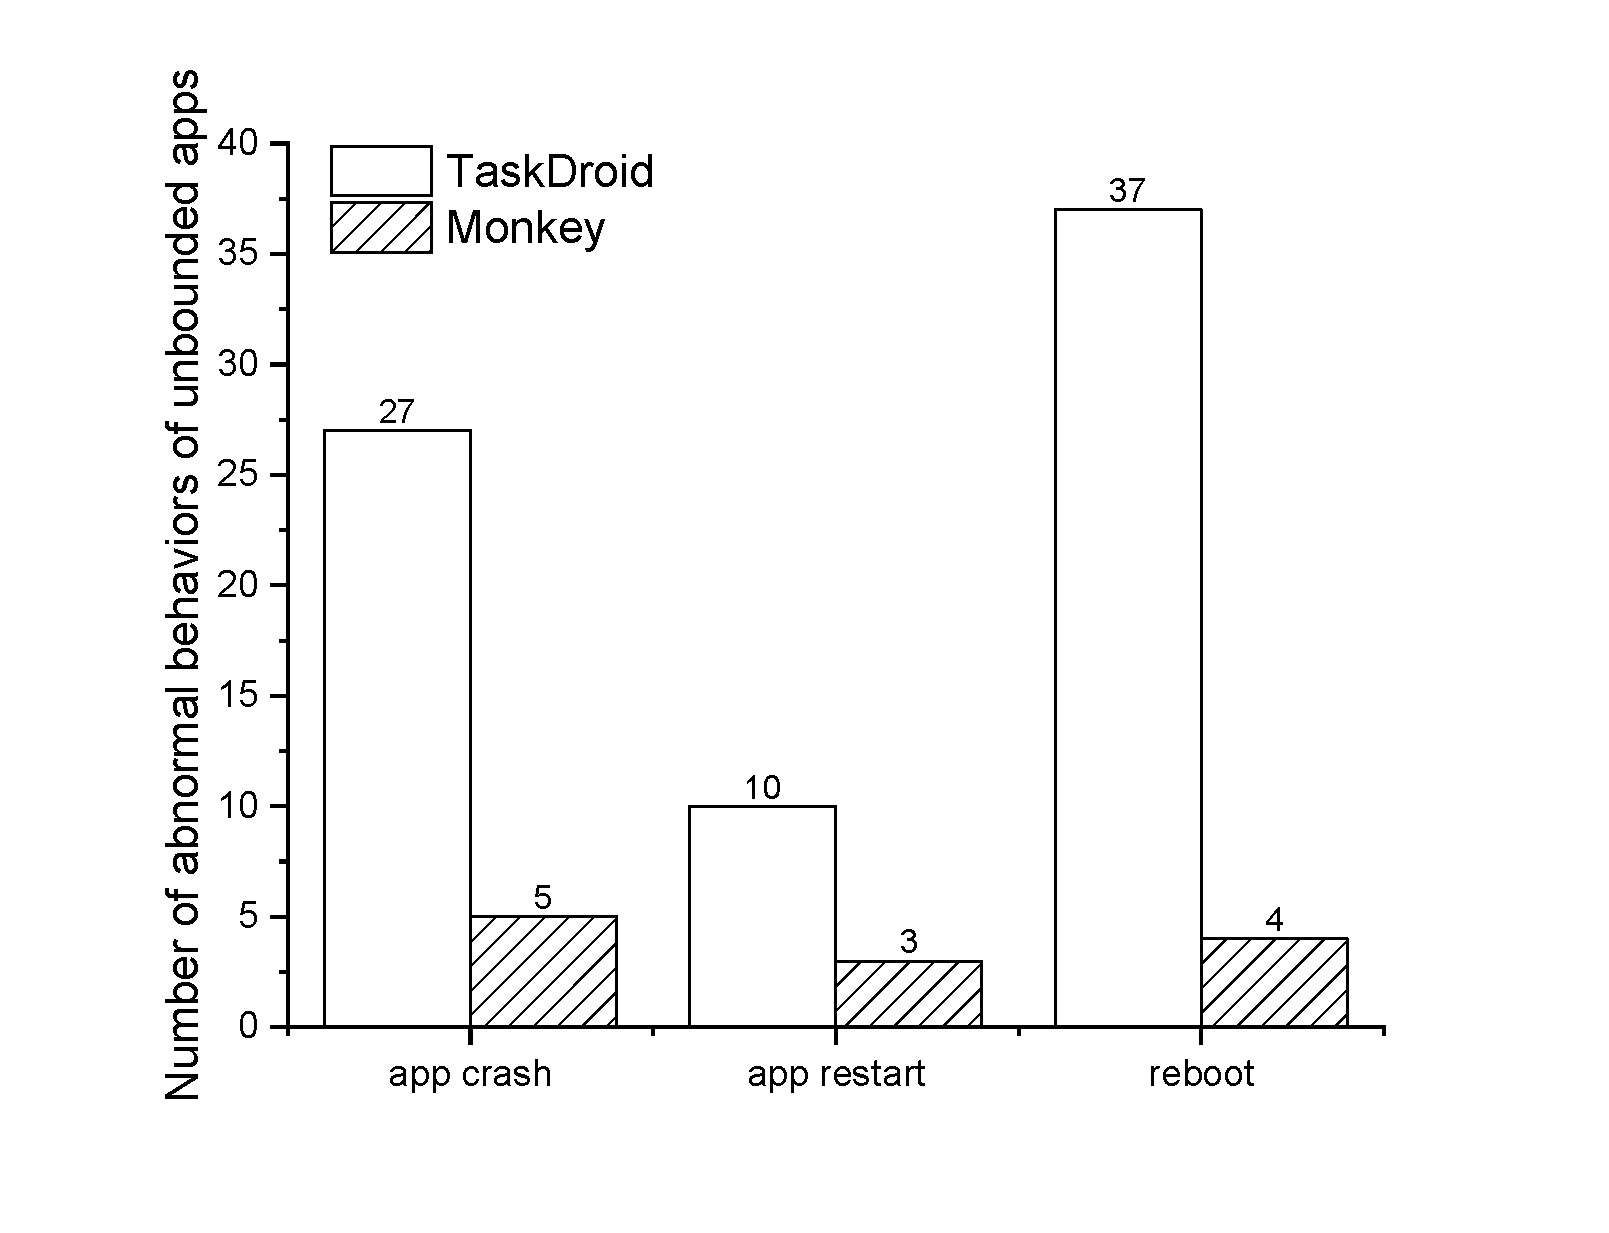
\includegraphics[width=8cm]{cmp-monkey.pdf}
	\caption{\revision{Number of abnormal behaviors of unbounded apps by TaskDroid and Monkey}}
	\label{fig:cmp-monkey}
\end{figure}


%\begin{table*}%[t]
%	\begin{center}   
%		\caption{Threat of unboundedness of popular commercial apps\label{tab:threatpop} }
%		\begin{tabular}{|c|c|c|c|c|c|}   
%			\hline   \textbf{Source} &\begin{tabular}{c}\textbf{unboundedness} \\ \textbf{problem}\end{tabular}&\textbf{Package name} & size(MB) &\begin{tabular}{c} \textbf{\#repetitions of} \\ {\bf the witness cycle}\end{tabular} & \textbf{Abnormal behavior} \\   
%			%
%			\hline   GooglePlay& task  & com.taobao.taobao & 151.0 & 66 & reboot  \\ 
%			\hline   GooglePlay& task  & com.jingdong.app.mall & 92.6 & 59 & reboot  \\ 
%			\hline   GooglePlay& task  & com.amazon.mShop.android.shopping & 73.8 & 73 & reboot  \\ 
%			\hline   GooglePlay& task  & com.contextlogic.wish & 21.9 & 63 & reboot  \\ 
%			\hline   GooglePlay& task  & com.google.android.youtube & 121.3 & 54 & reboot  \\ 
%			\hline   GooglePlay& task  & com.netflix.ninja & 100.6 & 76 & reboot  \\ 
%			\hline   GooglePlay& task  & com.instagram.android & 49.2 & 89 & reboot  \\ 
%			\hline   GooglePlay& task  & com.zhiliaoapp.musically & 167.8 & 65 & reboot  \\ 
%			\hline   GooglePlay& task  & com.facebook.katana & 74.2 & 96 & reboot  \\ 
%			\hline   
%		\end{tabular}   
%	\end{center}   
%\end{table*}

%%%%%%%%%%%%%%%%%%%%%%%%%%%%%%%%%%%%%%%%%%%%%%%%%%%%%%%%%%%%%%%%%%%%%%%%%%%%%%%%%%%%%%%%%%%%%%%%%%%%%%%%%%%%%%%%%%%%%



\subsubsection{Comparison of the impact of different model extractors}\label{sec:cmp}
%
We compare the impact of the following three model extractors on the effectiveness of the task/fragment container unboundedness problems: ICCBot$_{\AMASS}$, ICCBot, and ActExtractor, where ActExtractor is the model extractor from  \cite{HCWWY19}, where only activities were considered while fragments were ignored. 

We first run experiments to compare the capabilities of the three extractors to construct {\AMASS} models. The experiment results are in Figure~\ref{fig:cmp-extractor-model}, which include the numbers of models constructed by these extractors and the average number of transition rules in these models. From Figure~\ref{fig:cmp-extractor-model}, we can see that ICCBot$_{\AMASS}$ constructs more models than the other two extractors, since it is the only extractor that is able to construct models dynamically from APK files. Moreover, the average number of transition rules in the models constructed by ICCBot$_{\AMASS}$ is greater than the other two extractors, which is mainly because the models constructed dynamically by ICCBot$_{\AMASS}$ include much more transition rules than those constructed statically, since these apps are the ones that cannot be decompiled and normally large %popular 
commercial apps. 

\begin{figure}[htbp]
	\begin{minipage}[t]{0.49\linewidth}
		\centering
		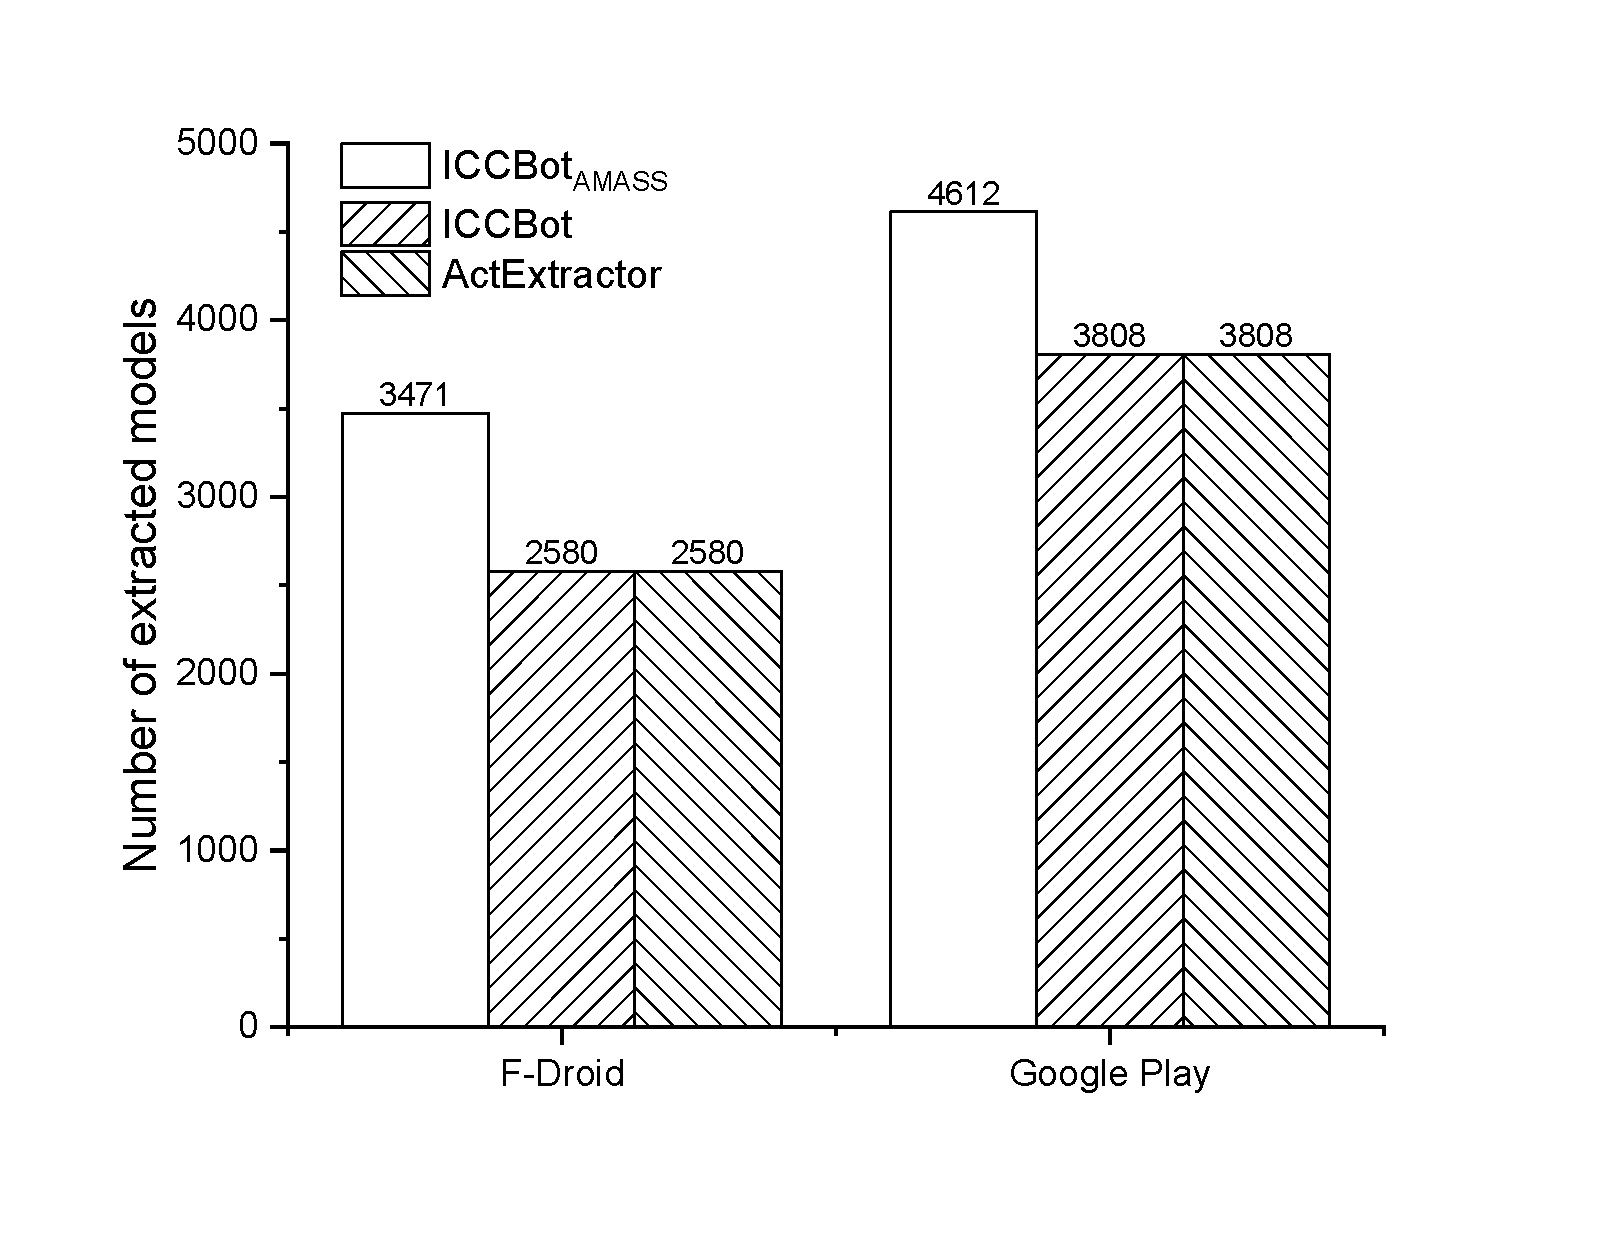
\includegraphics[width=3.2in]{model.pdf}
	\end{minipage}
	\begin{minipage}[t]{0.49\linewidth}
		\centering
		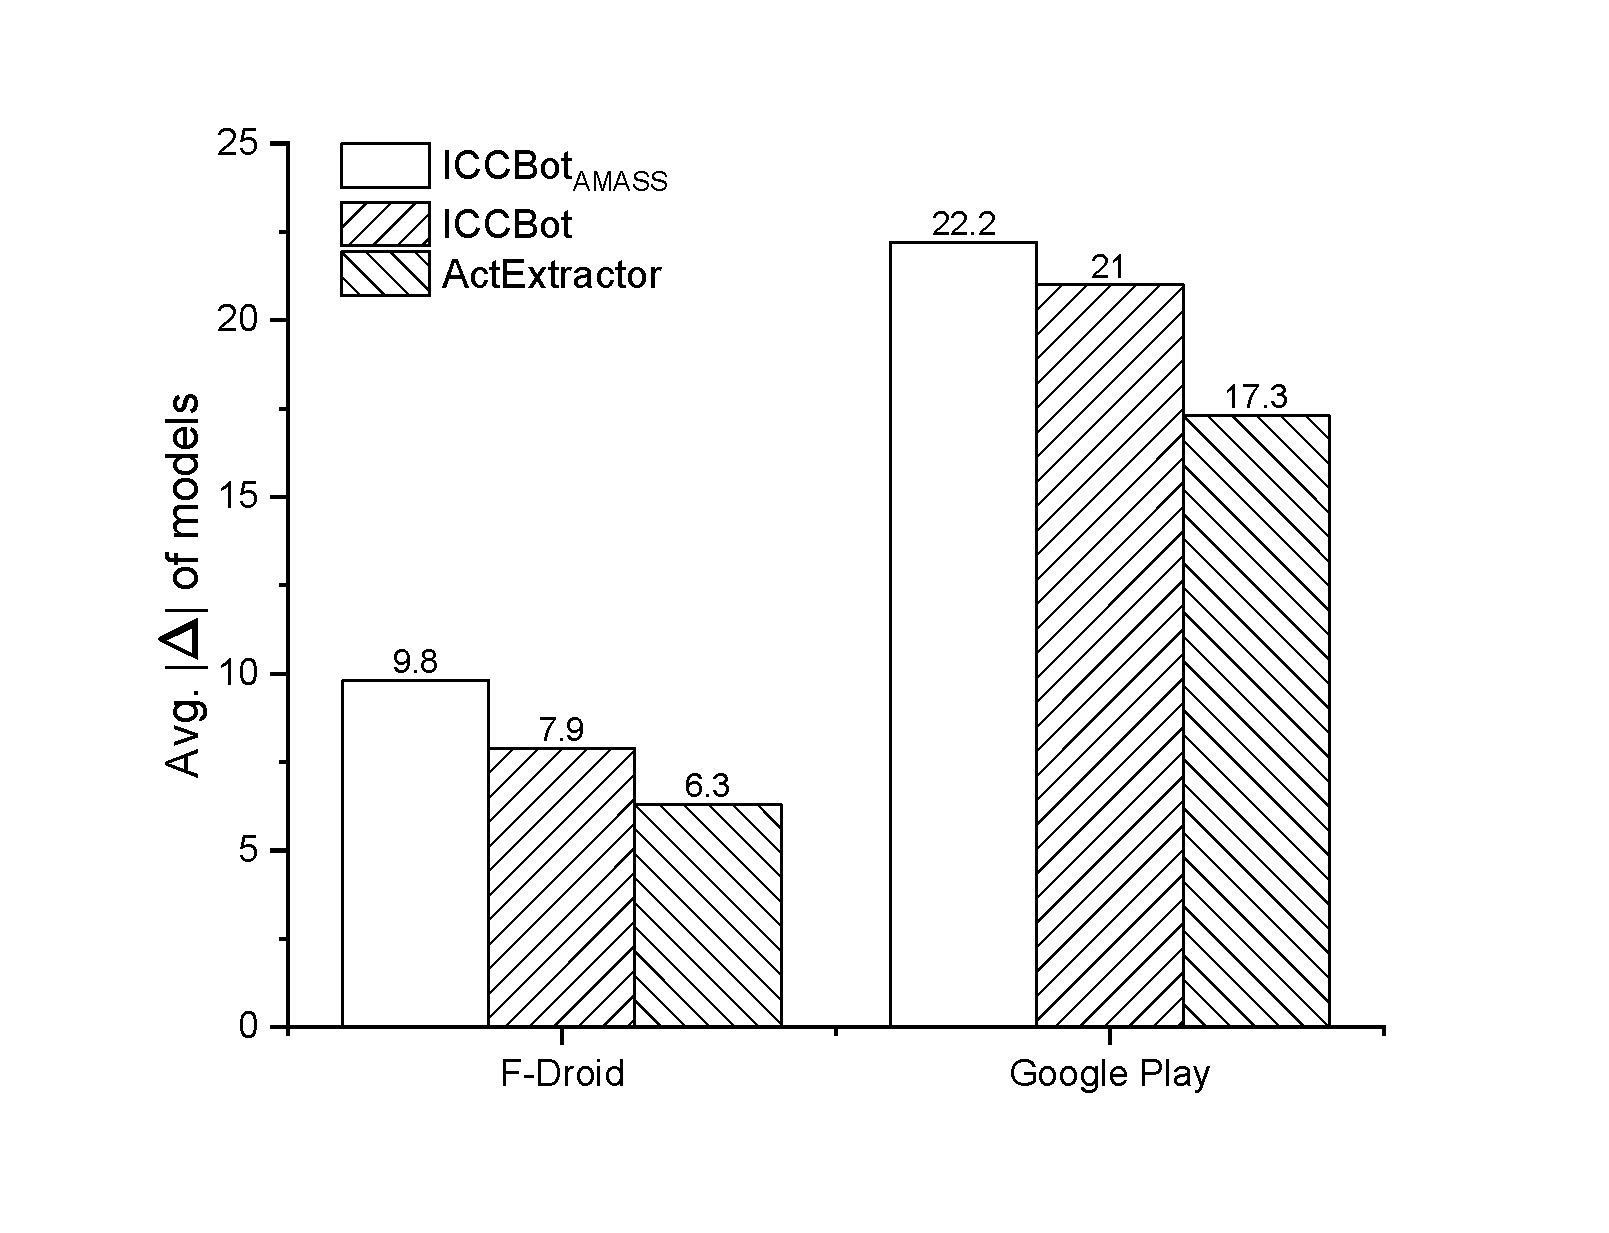
\includegraphics[width=3.2in]{delta.pdf}
	\end{minipage}
	\caption{Numbers of models extracted by different extractors and the average number of transitions in these models}
	\label{fig:cmp-extractor-model}
\end{figure}

%In this section, we conduct a comparison of model extraction and unboundedness using different {\AMASS} extractors, namely ICCBot$_{\AMASS}$, Extractor$_{\mathsf{APLAS}}$, and ICCBot. It is worth noting that Extractor$_{\mathsf{APLAS}}$ is the extractor utilized in \cite{HCWWY19}, which exclusively focuses on extracting activity transitions.

%Based on the observations from Figure~\ref{fig:cmp-extractor-model}, it is evident that ICCBot$_{\AMASS}$ exhibits the highest number of extracted models for both F-Droid apps and %Google Play apps, while the other two extractors yield the same results.
%The superior performance of ICCBot$_{\AMASS}$ can be attributed to its capability of extracting more models using dynamic {\sf AMASSExtractor}, which is not feasible with the other two extractors.
%Regarding the average size of transition rules in the extracted models, ICCBot$_{\AMASS}$ surpasses both ICCBot and Extractor$_{\mathsf{APLAS}}$. This can be attributed to the fact that ICCBot$_{\AMASS}$ and ICCBot are capable of extracting fragment transitions, while Extractor$_{\mathsf{APLAS}}$ lacks this functionality, and for the models extracted by the dynamic extractor, the average size of transition rules is greater than those extracted by the static extractor.

\begin{figure}[htbp]
	\begin{minipage}[t]{0.49\linewidth}
		\centering
		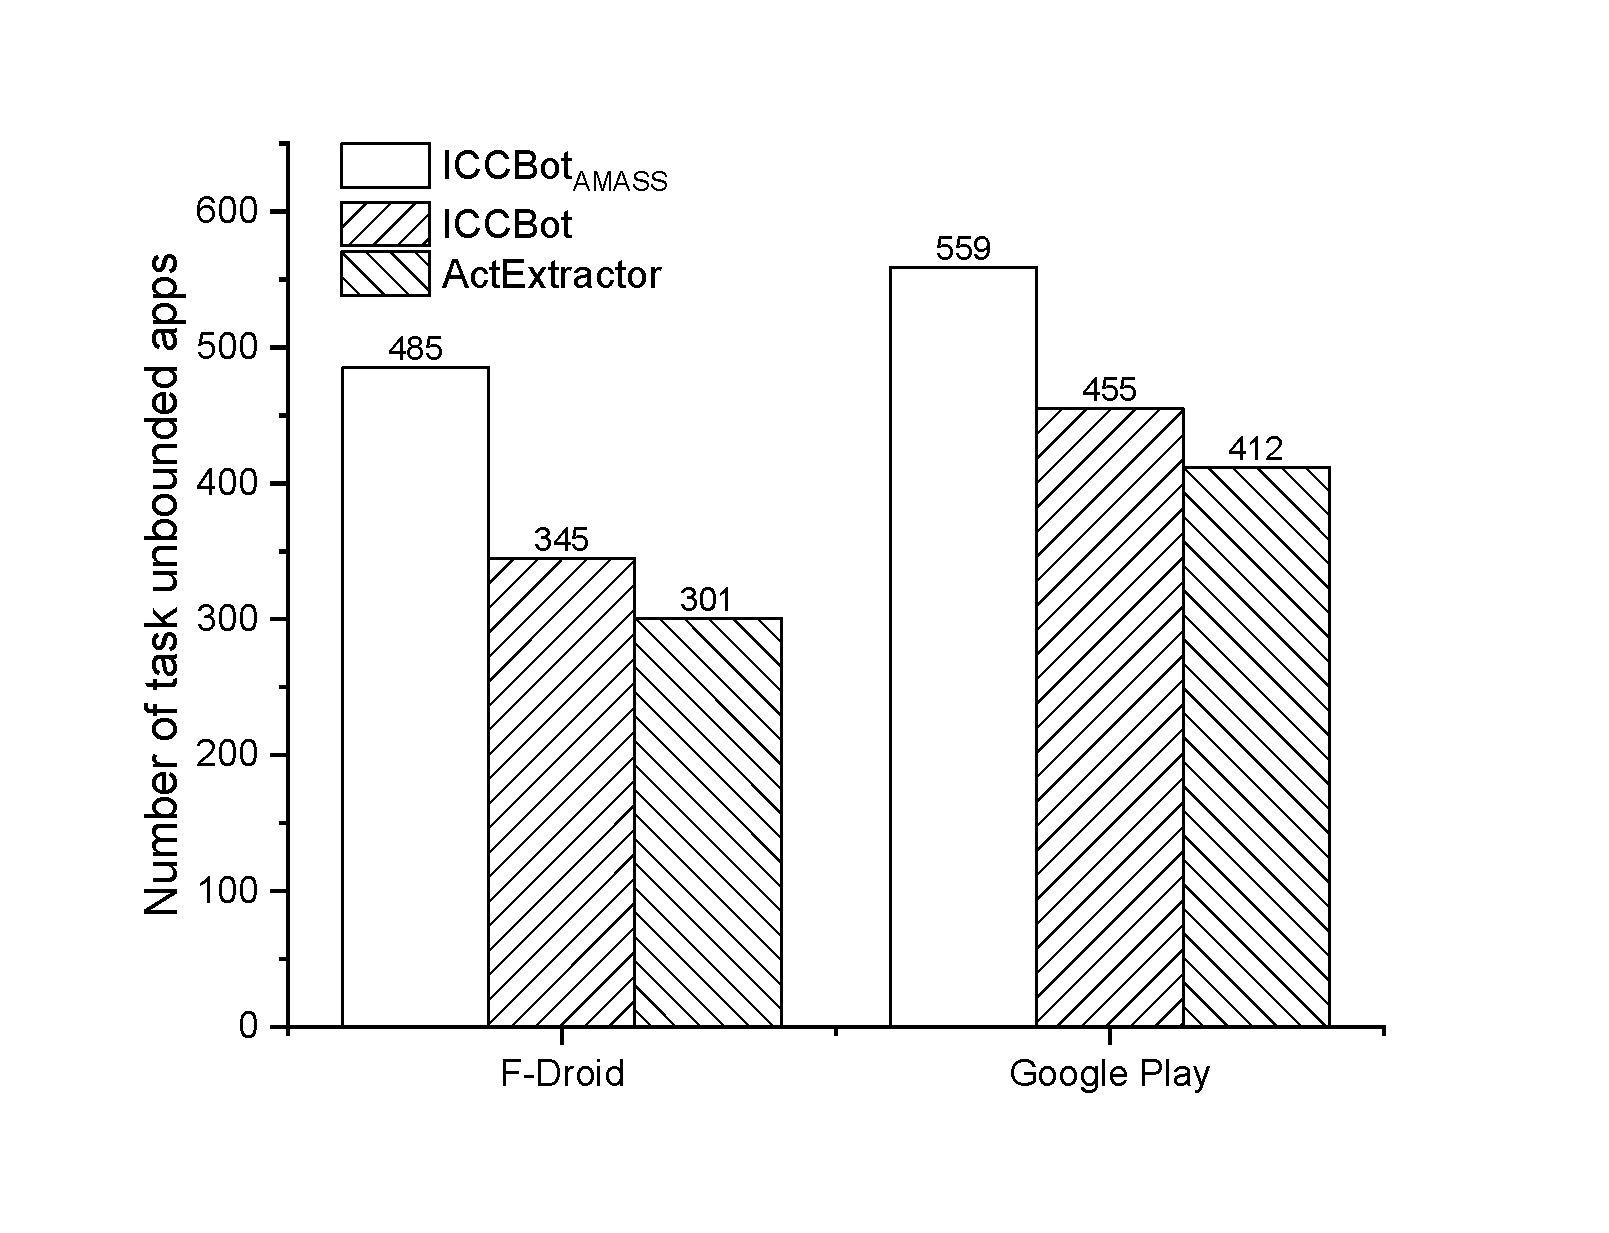
\includegraphics[width=3.2in]{task_ubd.pdf}
	\end{minipage}
	\begin{minipage}[t]{0.49\linewidth}
		\centering
		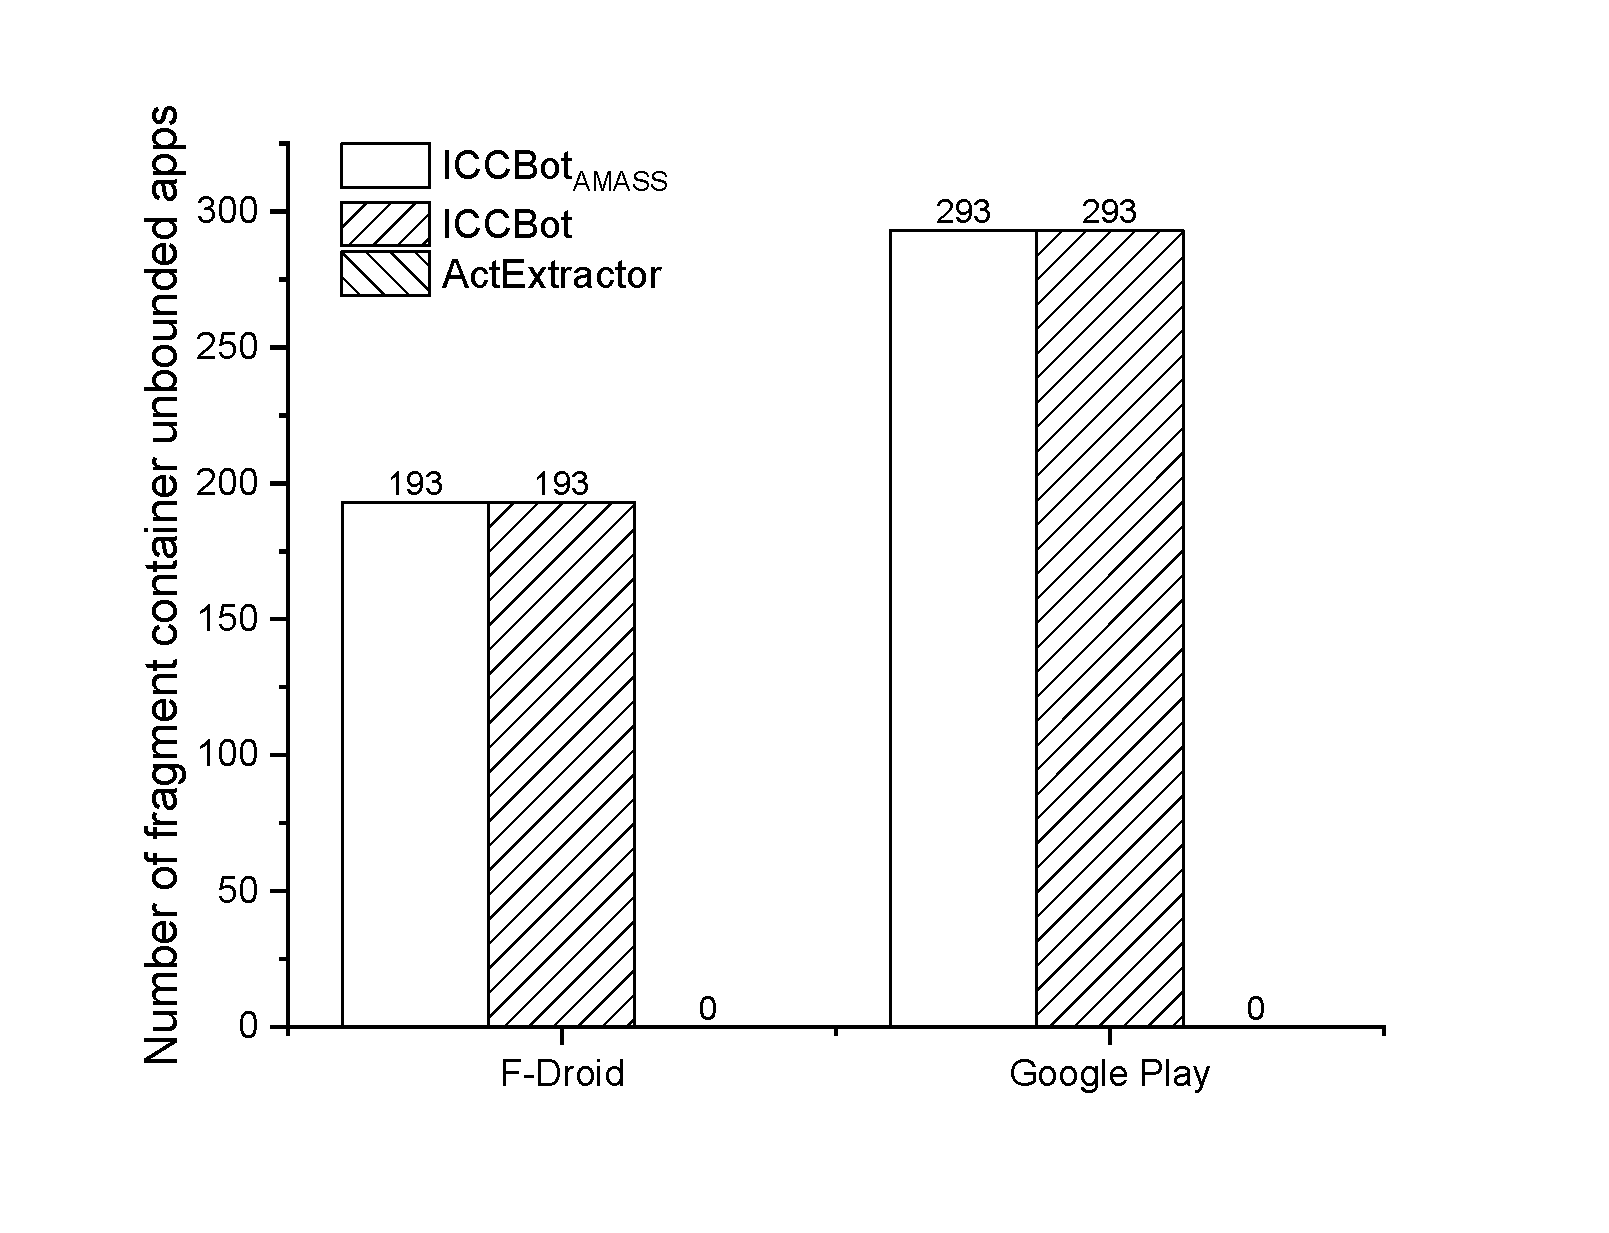
\includegraphics[width=3.2in]{frag_ubd.pdf}
	\end{minipage}
	\caption{Numbers of task/fragment container unbounded apps using different extractors}
	\label{fig:cmp-extractor-ubd}
\end{figure}


To compare the impact of different extractors on TaskDroid, for each app, we run {\sf AMASSAnalyzer} on the three models constructed by the three extractors for the app. We summarize the results in Figure~\ref{fig:cmp-extractor-ubd}, where we can see that the number of task unbounded apps is the greatest when ICCBot$_{\AMASS}$ is used. \revision{This is because ICCBot$_{\AMASS}$ extracts more models than the other two extractors since it utilizes the dynamic approach to extract the models from the commercial apps that cannot be decompiled. In Table~\ref{tab:threatpop}, by repeatedly executing the witness cycles, we confirm that among these apps whose models are constructed dynamically by ICCBot$_{\AMASS}$, 9 apps are indeed task unbounded. 
%	
Note that ICCBot and ActExtractor are unable to construct models from these apps since their APK files cannot be decompiled successfully by Soot.}
On the other hand, TaskDroid reports the same number of fragment container unbounded apps for ICCBot$_{\AMASS}$ and ICCBot. This is due to the fact that although ICCBot$_{\AMASS}$ extracts more information about fragments than ICCBot, e.g., the API addToBackstack(TS), the  information has no impact on our static analysis algorithm for the fragment container unboundedness problem (see Section~\ref{sec:static}). Moreover, no fragment unboundedness is reported for the models extracted by ActExtractor, since it only extracts the information for activities. 
%\jinlong{In conclusion, compared with \cite{HCWWY19}, TaskDroid detects more task unbounded apps and analyzes fragment container unbounded problem which \cite{HCWWY19} does not consider.}

%Based on Figure~\ref{fig:cmp-extractor-ubd}, it can be observed that ICCBot$_{\AMASS}$ exhibits the highest number of extracted models and the average size of transition rules. Consequently, ICCBot$_{\AMASS}$ detects a larger number of task unbounded apps compared to the other two extractors.  The discrepancy in the number of task unbounded apps detected between ICCBot and Extractor$_{\mathsf{APLAS}}$ can be attributed to the inability of Extractor$_{\mathsf{APLAS}}$ to extract fragment transitions. As a result, there are fewer transitions between activities, resulting in a lower number of task unbounded apps detected by Extractor$_{\mathsf{APLAS}}$ compared to ICCBot. 
%Regarding the number of fragment container unbounded apps detected, both ICCBot$_{\AMASS}$ and ICCBot yield the same results, as the dynamic {\sf AMASSExtractor} is unable to extract fragment transitions. However, Extractor$_{\mathsf{APLAS}}$ lacks the capability to extract fragment transitions, resulting in zero detections of fragment container unbounded apps by Extractor$_{\mathsf{APLAS}}$.


% \subsubsection{\revision{}}\label{sec:cross-app}
%%%%%%%%%%%%%%%%%%%%%%%%%%%%%%%%%%%%%%%%%%%%%%%%%%%%%%%%%%%%%%%%%%%%%%%%%%%%%%%%%%%%%%%%%%%%%%%%%%%%%%

\subsection{Validation of the  ``small number of tasks''  and ``small height of stacks''  hypotheses} \label{sec:hyp}

We validate the ``small number of tasks''  and ``small height of stacks''  hypotheses used in Section~\ref{sec:static}.
%
Recall that for the analysis of task unboundedness in Section~\ref{sec:static},  we hypothesize that only a small number $k$ of tasks are involved. 

We first evaluate the validity of the ``small number of tasks'' hypothesis for task unboundedness by varying  $k$ from $0$ to $3$ and checking the growth of the number of task unbounded apps detected by {\tool}. 
The experimental results are shown in Figure~\ref{fig:k}.
We observe that when $k$ is increased from $1$ to $2$, the number of task-unbounded apps increases only slightly.
Moreover, when $k$ is increased from $2$ to $3$, the number of task-unbounded apps keeps unchanged.
This suggests that, in order to identify those task-unbounded apps, a small $k$ suffices (in this case $k=2$). This also justifies our choice of $k$ in the static analysis of task unboundedness for {\AMASS} models.  This phenomenon is explained by the observation that for a majority of apps, %satisfy that 
the number of task affinities of their activities is small (or even equal to 1).
%
% \begin{figure}%[h]
% \centering
% 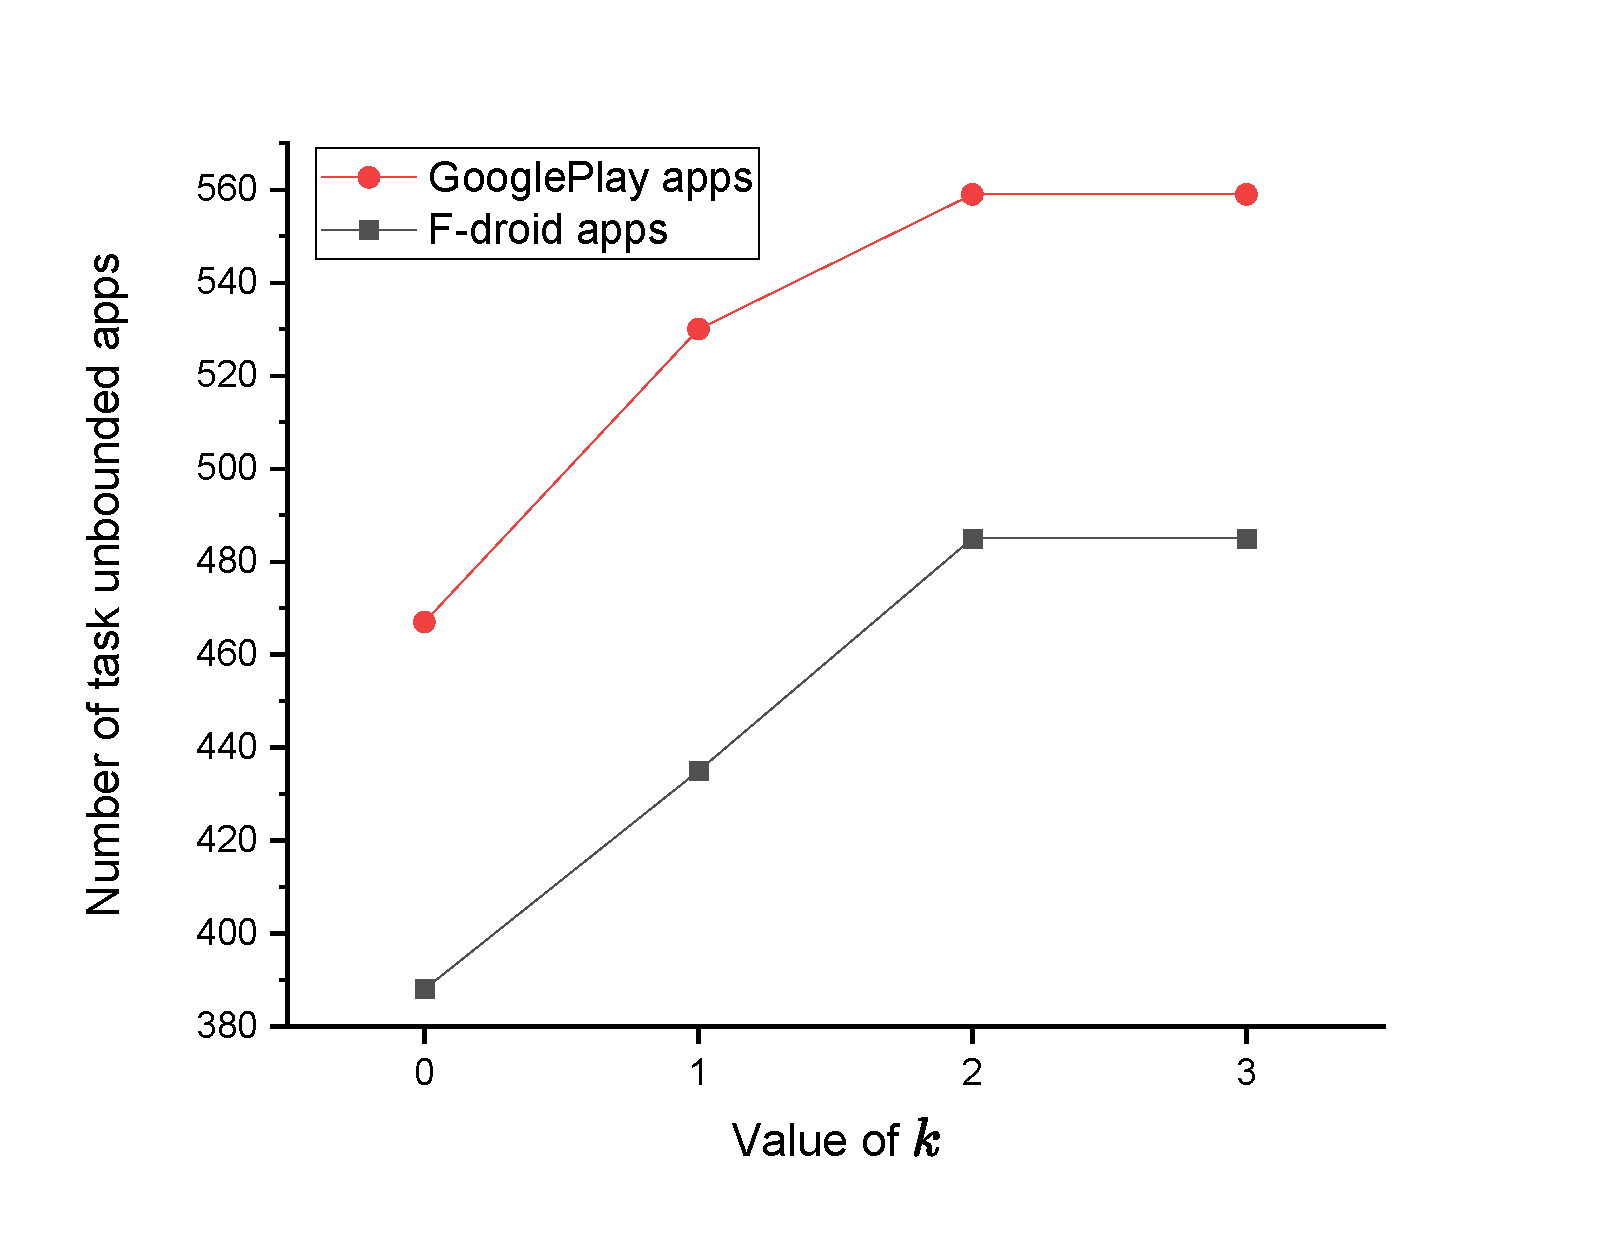
\includegraphics[scale=0.4]{k.pdf}
% \caption{Small number hypothesis: k}
% \label{fig:k}
% \end{figure}

Moreover, in Section~\ref{sec:static}, the height bound $\hbar = 6$ of stacks was used to generate the witnessing transition sequences for task unbounded and fragment container unbounded {\AMASS} models. We then carry out experiments to validate this ``small height of stacks'' hypothesis. 
The experiments proceed as follows: we first set $\hbar = 1$, use {\nuxmv} to generate the witnessing transition sequences for the  {\AMASS} models that are identified as ``task unbounded''  by TaskDroid, and count the number of models for which the witnessing transition sequences can be successfully generated. Then we experiment $\hbar=2$--$7$. % and do the same thing as for $\hbar = 2$. 
The results are summarized in Figure~\ref{fig-small-height}, where we can see that the number of models for which the witnessing transition sequences can be successfully generated grow when $\hbar$ is increased from $1$ to $6$, while keep unchanged when $\hbar$ is increased from $6$ to $7$. The results justify the ``small height of stacks'' hypothesis and our choice of $\hbar = 6$ in Section~\ref{sec:static}. 


%Recall that for the reachability analysis we hypothesize that the heights of involved tasks are bounded by a small number $\hbar$. Likewise, for the task boundedness analysis,  we hypothesize that only a small number $k$ of tasks are involved. In our experiments, we indeed set $\hbar$ to $4$ and $k$ to 2. In this section, we  aim to investigate whether these hypotheses are tenable. 
\begin{figure}[htbp]
\centering
\begin{minipage}[t]{0.48\textwidth}
\centering
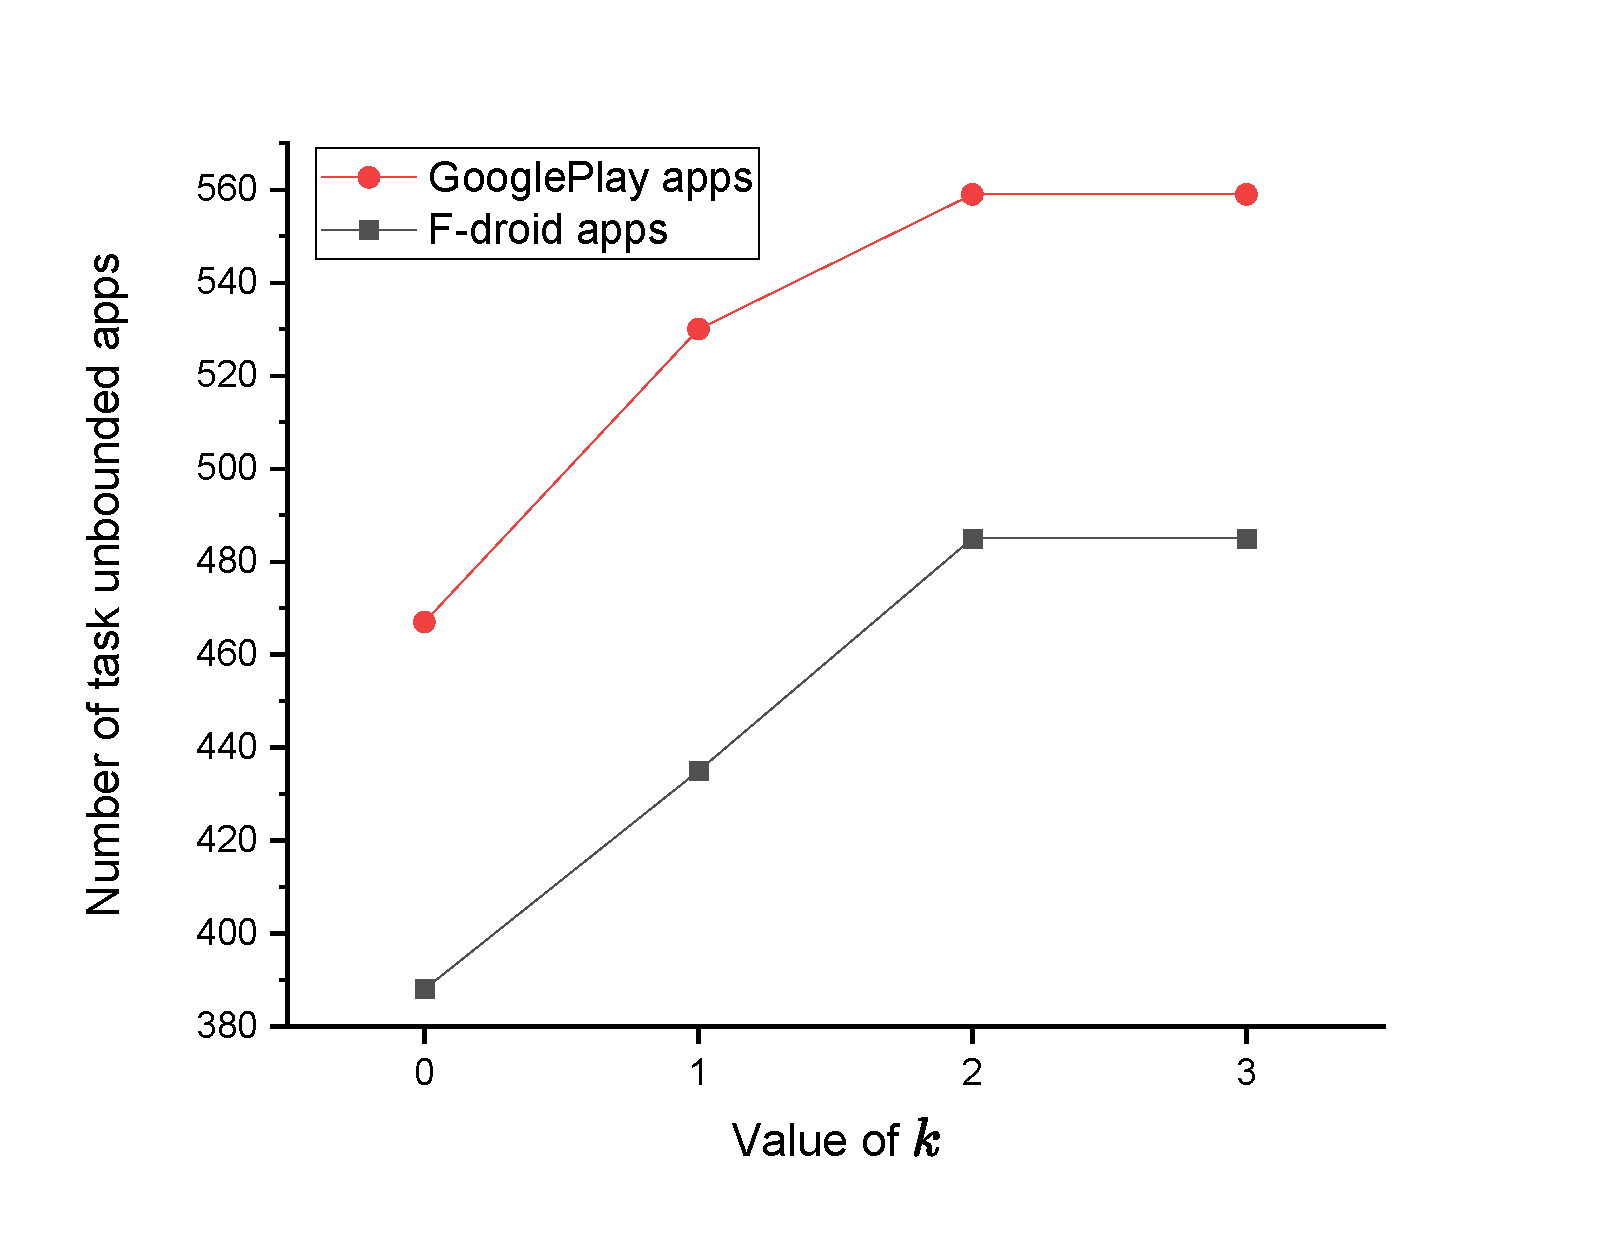
\includegraphics[width=8cm]{k.pdf}
\caption{``Small number of tasks'' hypothesis: $k$}
\label{fig:k}
\end{minipage}
\begin{minipage}[t]{0.48\textwidth}
\centering
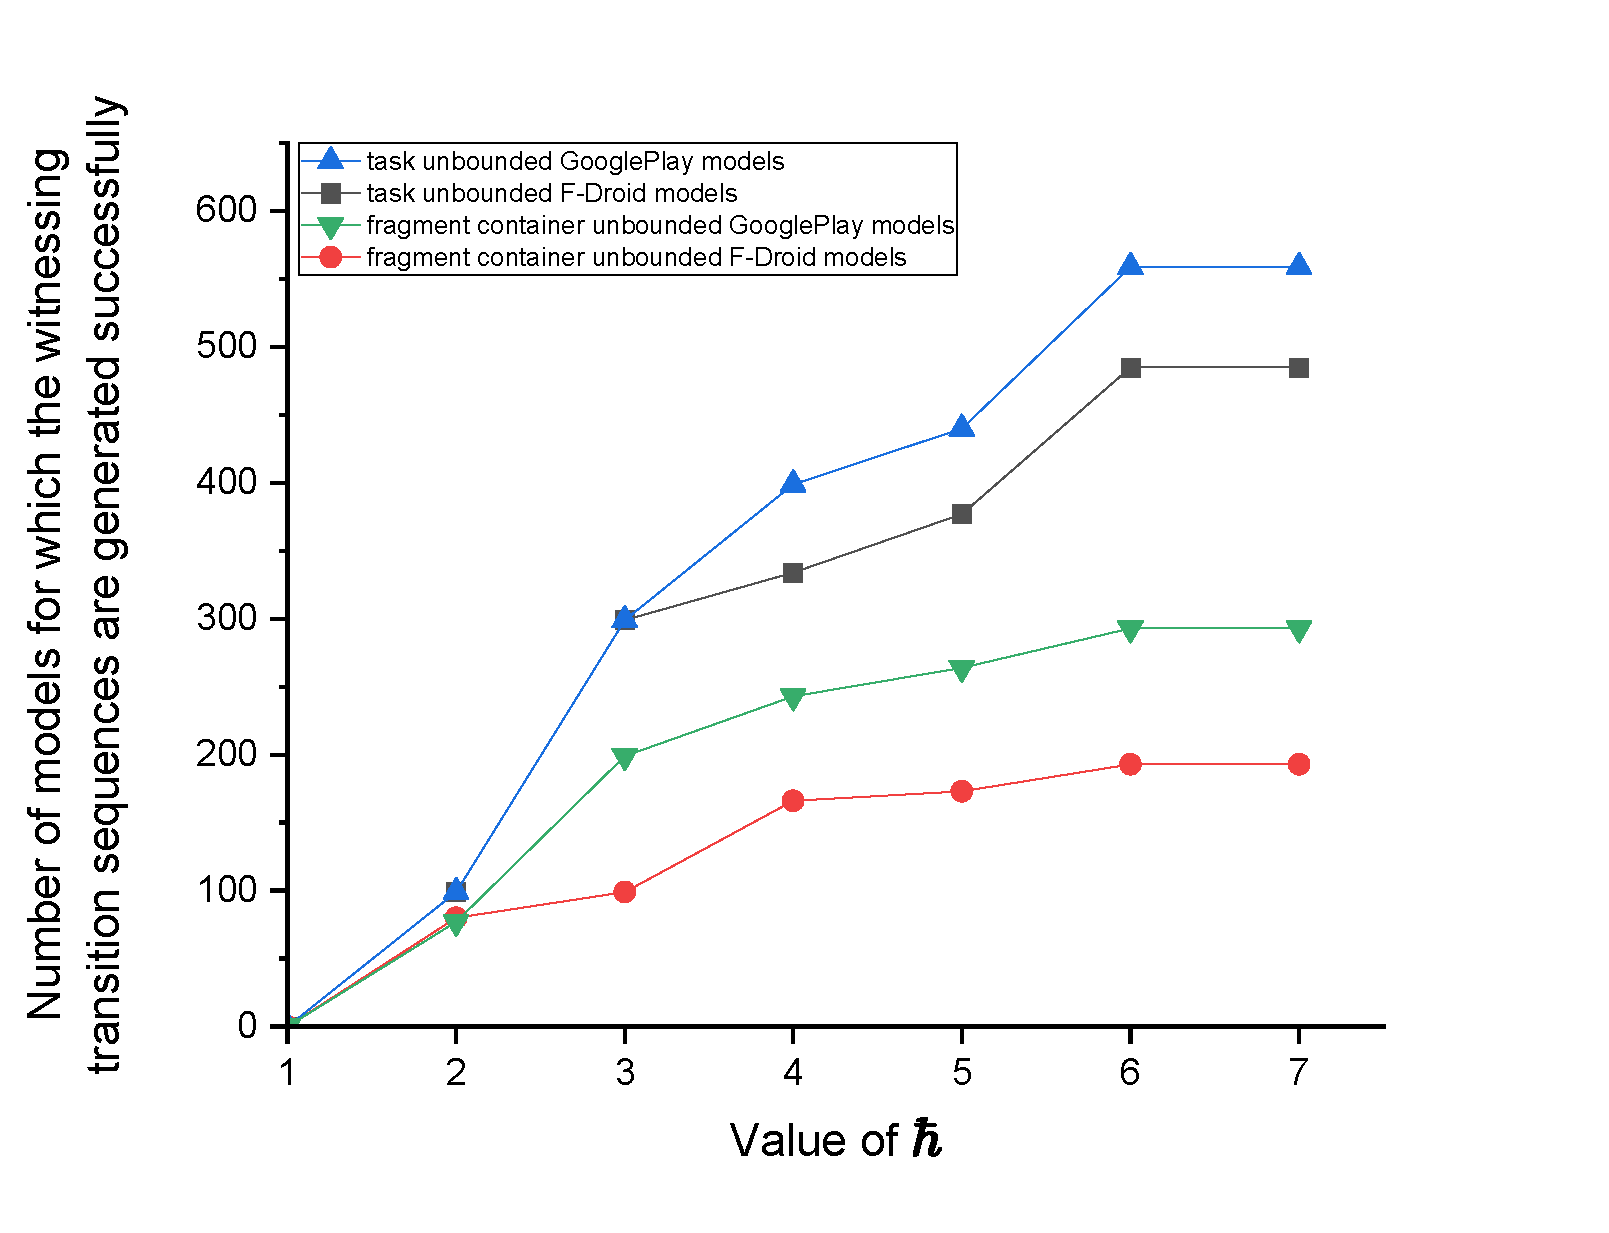
\includegraphics[width=8cm]{h.pdf}
\caption{``Small height of stacks'' hypothesis: $\hbar$}
\label{fig-small-height}
\end{minipage}
\end{figure}
	
% \begin{figure}%[h]
% \centering
% 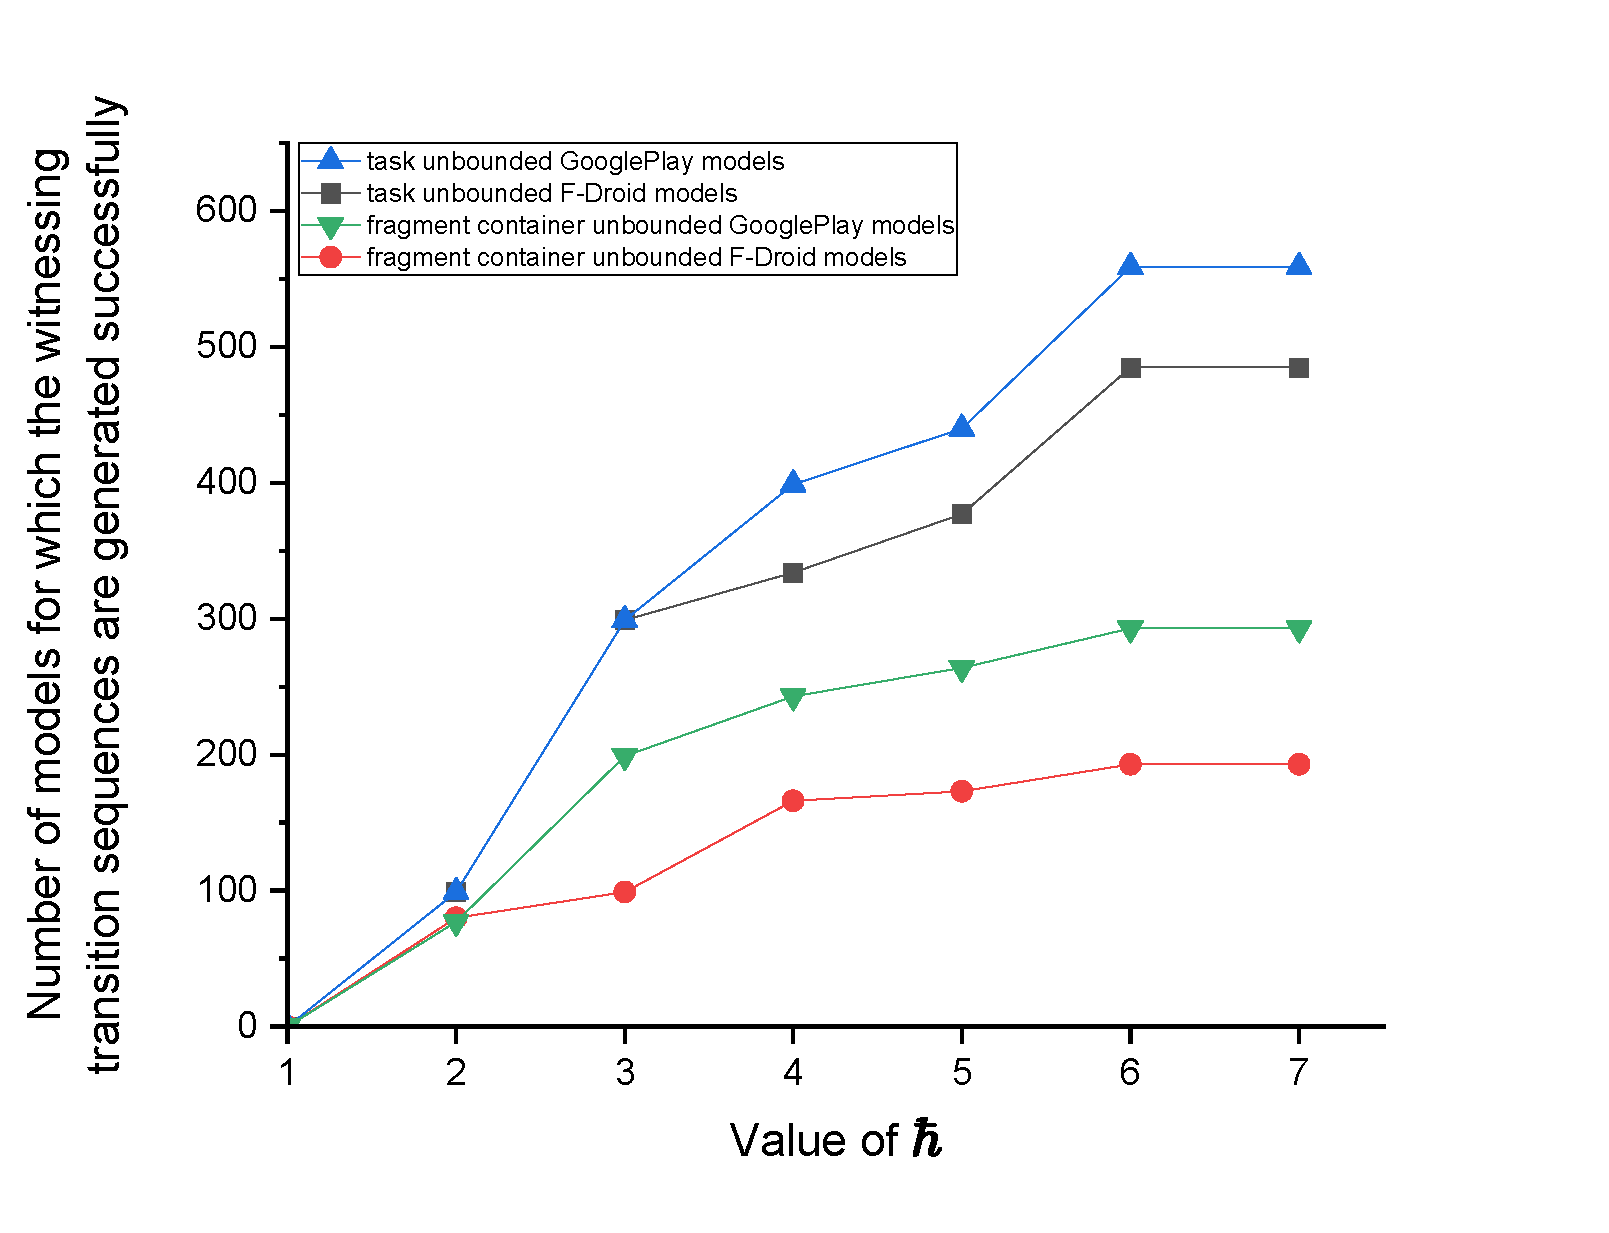
\includegraphics[scale=0.45]{h.pdf}
% \caption{``Small  height of stacks'' hypothesis}
% \label{fig-small-height}
% \end{figure}


%the number $k$ has little influence 
% obtain the conclusion that $k$ has little influence on the results, hence a small number $k$ can lead almost correct results. There are two reasons leading this conclusion, 1) there are nearly $90\%$ apps have only one single affinity in our bench mark, hence $k = 0$ can solve almost all of them. 2) there are nearly $70\%$ apps are acyclic which can lead to be stack bounded directly.



%the size means the average back pattern size of an activity in the bench mark, and 
%$k$ is the maximal stack height for each app. $\Delta_{size}$ means the difference of back pattern size of the same activity in the same app between the different value of $k$. Hence we can obtain the conclusion that there are little difference between $k = 4$ and $k = 6$, this is because the maximal stack height in most apps are not very large.

%Based on these results, we conclude that $\hbar$-reachability and $k$-task boundedness  provide sufficiently precise analysis results for reasonably small $\hbar$ or $k$.    

%We carry  out all experiments on a Linux server with a CPU of Intel\textsuperscript{\textregistered} Xeon\textsuperscript{\textregistered} Processor E5-2680 v4 at 2.40GHz and 64GB memory.

 

\hide{
\begin{table}%[htb]   
\begin{center}   
\begin{tabular}{|c|c|c|c|}   
    \hline   \textbf{Source} &\textbf{Extractor}  &\begin{tabular}{c}\textbf{\#Unbounded}\\ \textbf{models}\end{tabular} & \begin{tabular}{c} \#\textbf{witness cycles} \\ \textbf{per model}\end{tabular}  \\   
	\hline
    \multirow{3}{*}{F-Droid} &ICCBot$_{\AMASS}$ & 485/3,471(14.0\%) & 3.3\\
    \cline{2-4}    
     &ICCBot$_{\mhcancel{\frag}}$ & 416/3,471(12.0\%) & 3.1\\
    \cline{2-4}    
     &ICCBot & 332/2,580(12.9\%) & 3.0\\
	\hline
    \multirow{3}{*}{Google Play} &ICCBot$_{\AMASS}$& 559/4,612(12.1\%)&3.9\\
    \cline{2-4}    
     &ICCBot$_{\mhcancel{\frag}}$ & 512/4,612(11.1\%)&3.6\\
    \cline{2-4}    
     &ICCBot & 382/3,808(10.0\%)&3.4\\
\hline   
\end{tabular}   
\caption{Task Unboundedness under different extractors \label{tab:taskbound-model} }
\end{center}   
\end{table}

\begin{table}%[htb]   
\begin{center}   
\begin{tabular}{|c|c|c|c|}   
    \hline   \textbf{Source} &\textbf{Extractor}  &\begin{tabular}{c}\textbf{\#Unbounded}\\ \textbf{models}\end{tabular} & \begin{tabular}{c} \#\textbf{witness cycles} \\ \textbf{per model}\end{tabular}  \\   
	\hline
    \multirow{3}{*}{F-Droid} &ICCBot$_{\AMASS}$ & 193/2,580(7.5\%) & 2.5\\
    \cline{2-4}    
     &ICCBot$_{\mhcancel{\frag}}$ & 0/2,580(0\%) & 0\\
    \cline{2-4}    
     &ICCBot & 193/2,580(7.5\%) & 2.5\\
	\hline
    \multirow{3}{*}{Google Play} &ICCBot$_{\AMASS}$& 293/3,808(7.7\%)&3.0\\
    \cline{2-4}    
     &ICCBot$_{\mhcancel{\frag}}$ & 0/3,808(0\%)&0\\
    \cline{2-4}    
     &ICCBot & 293/3,808(7.7\%)&3.0\\
\hline   
\end{tabular}   
\caption{Fragment Container Unboundedness under different extractors \label{tab:fragbound-model} }
\end{center}   
\end{table}
}

\hide{
\begin{table}%[htb]   
\begin{center}   
\begin{tabular}{|c|c|c|c|c|c|}   
    \hline   \textbf{Source} & \textbf{Unbounded} & \textbf{Android 6.0} & \textbf{Android 7.0}  & \textbf{Android 8.0-10.0} &\textbf{Android 11.0-13.0} \\   
    \hline   \multirow{2}{*}{F-Droid} & Task & 490 & 484 & 486 & 485 \\
    \cline{2-6}    & Fragment Container & 193 & 193 & 193 & 193\\
    \hline \multirow{2}{*}{Google Play} & Task & 568 & 555 & 562 & 559 \\
    \cline{2-6}    & Fragment Container & 293 & 293 & 293 & 293 \\
\hline   
\end{tabular}   
\caption{\revision{Unboundedness under different Android versions \label{tab:bound} }}
\end{center}   
\end{table}
}

\hide{
\begin{table}%[htb]   
\begin{center}   
\begin{tabular}{|c |c |c |c |c |c |c |c|c|}   
    \hline    
    \multirow{2}{*}{\textbf{Source}} & \multirow{2}{*}{\textbf{Extractor}}  &\multicolumn{3}{c|}{\textbf{Avg/Max. size of models}} & \multirow{2}{*}{\textbf{\# extracted  models}} \\   
    \cline{3-5}    
    && $|\act|$& $|\frag|$ & $|\Delta|$ &   \\ 
    \hline   
    \multirow{3}{*}{F-Droid} &ICCBot$_{\AMASS}$ &  5.2/70& 0.4/16 & 9.8/475 &  3,471  \\ 
    \cline{2-6}    
     &ICCBot$_{\mhcancel{\frag}}$ &  5.2/70& 0/0 & 6.3/332 &  3,471  \\ 
    \cline{2-6}    
     &ICCBot &  4.9/70& 0.5/16 & 6.9/369 &  2,580  \\ 
    \hline   
    \multirow{3}{*}{Google Play}&ICCBot$_{\AMASS}$  & 7.8/509&0.8/121&22.2/1,956 & 4,612  \\  
    \cline{2-6}    
     &ICCBot$_{\mhcancel{\frag}}$ & 7.8/509&0/0&17.3/1,234 & 4,612  \\  
    \cline{2-6}    
     &ICCBot  & 7.1/509&1.0/121&18.9/1,557 & 3,808  \\  
    % \hline   
    % \multirow{2}{*}{ICCBot} &F-Droid &  3.6/70& 0.4/16 & 5.9/369 &  2,580  \\ 
    % \cline{2-6}    
    %  &Google Play  & 7.1/509&1.0/121&21.0/1956 & 3,808  \\  
\hline   
\end{tabular}   
\caption{Comparison with AMASSExtractors \label{tab:extractor} }
\end{center}   
\end{table}
}



\section{Conclusion} \label{sec:conc}
In this paper, we have formalized the semantics of the Android multitasking mechanism by a new model {\AMASS}, which have been validated against the actual behaviors of Android systems. Based on the semantics, we provide new static analysis algorithms for detecting potential task unboundedness and fragment container unboundedness vulnerabilities. We have implemented a static analysis tool TaskDroid. The experiments show that TaskDroid is able to discover the task-unboundedness and fragment-container-unboundedness vulnerabilities for many open-source and commercial Android apps, which can be exploited to produce abnormal behaviors, e.g. black screen, app crash or even device reboot. 

The formal semantics of the {\AMASS} model defined in this paper is valuable for both the developers of Android apps and the researchers on the analysis and testing of Android apps. 
\begin{itemize}
\item the developers can read the concise and precise semantics of the {\AMASS} model, instead of the source code of the Android OS, to understand the Android activity-fragment multitasking mechanism. % in a much faster and easier way. 
%
\item Compared to the various models (e.g. activity transition graphs) in literature,  the {\AMASS} model provides refined modeling of the Android activity-fragment multitasking mechanism, and can be utilized to improve the accuracy of the analysis and testing of Android apps. 
%
\item The task unboundedness issue identified in this paper is a novel type of security threats for Android apps, contributing to %and provides a different angle for developers to understand the 
the understanding the security aspect of Android UI design. 
\end{itemize}

%From our formal semantics of the Android multitasking mechanism, app developers can gain a clear understanding of how task affinities, launch modes, intent flags, and fragment transactions influence the behaviors of the back stack,facilitating better app development. This is particularly valuable as the official documentation is complex and challenging to comprehend. Furthermore, researchers can also utilize the AMASS model to propose more advanced static analysis algorithms for complex security issues related to the Android multitasking mechanism.

For the future work, more problems in static analysis %are worth studying which 
can %significantly 
benefit from the formalized multi-tasking semantics. 
Moreover, we believe that {\AMASS} is a fundamental model in Android UI research which deserves a thorough theoretical investigation.
%%%%%%%%%%%%%%%%%%%%%%%%%%%%%%%%%%%%%%%%%%%%%%%%%%%%%%%%%%%%%%%%%%%%%%%%%%%%%%%%%%%%%%%%%%%%%%
\bibliographystyle{alpha}
\bibliography{references}

\newpage
%%%%%%%%%%%%%%%%%%%%%%%%%%%%%%%%%%%%%%%%%%%
\appendix
%!TEX root = main.tex

\section{Semantics of $A \xrightarrow{\finishstart(\phi)} B$ for {$\LMAOAMASS$}}\label{app-finishstart-lmaoamss}
In the sequel, assuming that $\Mm$ is an $\LMAOAMASS$.

Let $\rho = (\Omega_1,\cdots,\Omega_n)$ be a configuration with  $\Omega_i = (S_i, A_i, \zeta_i)$ for each $i\in[n]$, and $S=[B_1,\cdots,B_m]$ be a task. 
% Let $(\rho,b)$ be a configuration with $\rho = (\Omega_1,\cdots,\Omega_n)$ and $\Omega_i = (S_1,A_i,\zeta_i)$ for each $i\in[n]$, and $S=[B_1,\cdots,B_m]$ be a task. 
The following additional auxiliary function $\rmact(\rho,i, j)$ is defined for $\finishstart$.
\begin{itemize}
    \item let $1 \le i \le n$, $S_i = [C_1, \cdots, C_l]$ and $1 \le j \le l$, then $\rmact(\rho,i, j) = (\Omega_1,\cdots,\Omega_{i-1},(S_i',A_i,\zeta_i),\Omega_{i+1},\cdots,\Omega_n)$ if $l>1$, where $S_i' = [C_1,\cdots, C_{j-1}, C_{j+1},\cdots, C_l]$, and $\rmact(\rho,i, j) = (\Omega_1,\cdots,\Omega_{i-1},\Omega_{i+1},\cdots,\Omega_n)$ otherwise.
\end{itemize}

We present the semantics of the transition rules $A \xrightarrow{\finishstart(\phi)} B$.

\smallskip
\noindent \fbox{$\lmd(B) = \STD$}
	\begin{itemize}
		\item If $\lmd(A) \neq \SIT$, then $\rho'= \rmact(\push(\rho,B), 1, 2)$.
		%
		\item If $\lmd(A) = \SIT$, then
    		\begin{itemize}
                \item if $\getrealtsk(\rho,B) = S_i$ and $\zeta_i\neq\mainflag$, then $\rho'=\rmact(\mvtsktop(\rho, i), 2, 1)$,
                \item if $\getrealtsk(\rho,B) = S_i$ and $\zeta_i = \mainflag$, or $\getrealtsk(\rho,B) = *\wedge \gettsk(\rho,B) = S_i$, \\then $\rho'=\rmact(\push(\mvtsktop(\rho, i),B), 2, 1)$,
    			\item if $\gettsk(\rho, B)=*$, then $\rho'= \rmact(\newtsk(\rho, B, \STK), 2, 1)$.
    		\end{itemize}
	\end{itemize}

\noindent  \fbox{$\lmd(B) = \STP$}
	\begin{itemize}
		\item  If $\lmd(A) \neq \SIT$, then
        \begin{itemize}
            \item if $A = B$, then $\rho' = \rmact(\rho, 1, 1)$,
            \item otherwise, $\rho' = \rmact(\push(\rho, B), 1, 2)$.
        \end{itemize}
		%
		\item If $\lmd(A) = \SIT$, then
    		\begin{itemize}
                \item if $\getrealtsk(\rho,B) = S_i$ and $\zeta_i\neq\mainflag$, then $\rho'=\rmact(\mvtsktop(\rho, i), 2, 1)$,
                \item if $\getrealtsk(\rho,B) = S_i$ and $\zeta_i = \mainflag$, or $\getrealtsk(\rho,B) = *\wedge \gettsk(\rho,B) = S_i$, 
                \begin{itemize}
                    \item if $\topact(S_i) = B$, then $\rho' = \rmact(\mvacttop(\rho,i), 2, 1)$,
                    \item otherwise $\rho'=\rmact(\push(\mvtsktop(\rho, i),B), 2, 1)$,
                \end{itemize}
                % then $\rho'=\push(\mvtsktop(\rho, i),B)$,
    			\item if $\gettsk(\rho, B)=*$, then $\rho'= \rmact(\newtsk(\rho,B, \STK), 2, 1)$.
    		\end{itemize}
	 \end{itemize}
	
\noindent \fbox{$\lmd(B) = \SIT$}
\begin{itemize}
	\item If $\getrealtsk(\rho, B) = S_1$, then $\rho' = \rmact(\rho, 1, 1)$.
	\item If $\getrealtsk(\rho, B) = S_i$ and $i > 1$, then $\rho' = \rmact(\mvtsktop(\rho, i), 2, 1)$.
	\item If $\getrealtsk(\rho, B) = *$, then $\rho' = \rmact(\newtsk(\rho, B,\SIT), 2, 1)$.
\end{itemize}

\noindent  \fbox{$\lmd(B) = \singletask$}
\begin{itemize}
	\item If $\getrealtsk(\rho, B) = S_i$, or $\getrealtsk(\rho,B) = *\wedge\gettsk(\rho,B) = S_i$ then
	\begin{itemize}
		\item if $i = 1$,
		\begin{itemize}
			\item if $B \not \in S_i$, then $\rho' = \rmact(\push(\rho, B), 1, 2)$,
			\item if $B \in S_i$, 
			\begin{itemize}
				\item if $\topact(\rho) = B$, then $\rho' = \rmact(\rho, 1, 1)$,
				\item if $\topact(\rho) \neq B$, then $\rho' = \clrtop(\rho, B)$,
			\end{itemize}
		\end{itemize}
		\item if $i > 1$,
		\begin{itemize}
			\item if $B \not \in S_i$, then $\rho' = \rmact(\push(\mvtsktop(\rho, i), B), 2, 1)$,
			\item if $B \in S_i$, 	then $\rho' =  \rmact(\clrtop(\mvtsktop(\rho, i), B), 2, 1)$.
		\end{itemize}
	\end{itemize}
\item If $\gettsk(\rho, B) = *$, then $\rho' = \rmact(\newtsk(\rho, B,\STK), 2, 1)$.
\end{itemize}

\section{Semantics of {$\IFAOAMASS$}}\label{app-ifaoamass}

In the sequel, assuming that $\Mm$ is an $\IFAOAMASS$.
% we present the semantics of the transition rules $A \xrightarrow{\finishstart(\phi)} B$.
Firstly, we need adapt the concept of configurations as follows:
A configuration of $\Mm$ is 
% still encoded as a sequence
encoded as a pair $(\rho, b)$, where $b \in \{\nohflag, \neg \nohflag\}$ and 
$\rho=(\Omega_1,\cdots,\Omega_n)$ such that for each $i \in [n]$, $\Omega_i = (S_i, A_i, \zeta_i)$, where $S_i \in \act^*$ is a task, $A_i \in \act$ is the real activity of $S_i$, but $\zeta_i \in \{\mainflag, \ntkflag, \ndmflag\}$. Intuitively, 
% $b$ denotes whether the topmost activity is started with $\nohflag$ or not, 
$\ntkflag$ in $\zeta_i$ plays the same role as $\STK$ in $\LMAOAMASS$, and $\ndmflag$ is added for the intent flag $\ndmflag$, moreover, $\SIT$ disappears since in $\IFAOAMASS$, the launch modes of all activities are assumed to be $\STD$.
% A configuration of $\Mm$ is encoded as a pair $(\rho, b)$, where $b \in \{\nohflag, \neg \nohflag\}$. Intuitively, $b$ denotes whether the topmost activity is started with $\nohflag$ or not.

Let us define the semantics of $\Mm$ by a relation 
% $\rho \xrightarrow[\Mm]{\startactivity(\phi)} \rho'$ with $\phi \models \neg \tohflag \wedge \neg \nohflag$.
$\rho \xrightarrow[\tau]{\Mm} \rho'$ with $\tau = A \xrightarrow{\alpha(\phi)} B$.
Let us consider the subcase $\phi \models \neg \tohflag$ first.

\smallskip
\noindent \fbox{$\phi \models \neg \ntkflag\wedge\neg\ndmflag$}
	\begin{itemize}
		\item If $\phi \models \ctpflag$ and $B \in \toptsk(\rho)$, then 
		\begin{itemize}
			\item if $\topact(\rho) \neq B$, then $\rho' = \clrtop(\rho, B)$, moreover, 
			\begin{itemize}
			\item if $\phi \models \neg \stpflag$, then $b' = \nohflag$ iff $\phi \models \nohflag$, 
			\item otherwise, $b' = \neg \nohflag$,
			\end{itemize}
			\item if $\topact(\rho) = B$, 
			\begin{itemize}
					\item if $\phi \models \stpflag$, then
					\begin{itemize}
						\item if $\alpha = \startactivity$, then $\rho' = \rho$ and $b' = b$,
						\item if $\alpha = \finishstart$, then $\rho' = \rmact(\rho, 1, 1)$ and $b' = \neg \nohflag$,
					\end{itemize}
					\item if $\phi \models \neg \stpflag$, then $\rho' = \rho$ and $b' = \nohflag$ iff $\phi \models \nohflag$.
				% \item if $\alpha = \startactivity$, then $\rho' = \rho$,
				% \item if $\alpha = \startactivity$, then $\rho' = \rho$, moreover, 
				% \begin{itemize}
				% 	\item if $\phi \models \neg \stpflag$, then 
				% 	$b' = \nohflag$ iff $\phi \models \nohflag$, 
				% 	\item otherwise, $b' = b$,
				% \end{itemize}
				% \item if $\alpha = \finishstart$, then $\rho' = \rmact(\rho, 1, 1)$ and $b' = \nohflag$ iff $\phi \models \nohflag$, 
			% \end{itemize}
			% \end{itemize}
			% $\rho' = \rho$, moreover,
		\end{itemize}
		\end{itemize}
		\item If $\phi \models \ctpflag$ and $B \notin \toptsk(\rho)$, then $b' = \nohflag$ iff $\phi \models \nohflag$, moreover,
		\begin{itemize}
			\item if $b = \neg \nohflag$ and $\alpha = \startactivity$, then $\rho' = \push(\rho, B)$, 
			\item otherwise, $\rho' = \rmact( \push(\rho, B), 1, 2)$. 
		\end{itemize}
		\item If $\phi \models \neg \ctpflag$, then
		\begin{itemize}
			\item if $\phi \models \rtfflag$ and $B \in \toptsk(\rho)$, then
			\begin{itemize}
				\item if $\topact(\rho) \neq B$, then $b' = \neg \nohflag$, moreover, 
				\begin{itemize}
					\item if $b = \neg \nohflag$ and $\alpha = \startactivity$, then $\rho'= \mvacttop(\rho, B)$, 
					\item otherwise, $\rho' = \rmact(\mvacttop(\rho, B), 1, 2)$, 
				\end{itemize}
				\item if $\topact(\rho) = B$, 
				\begin{itemize}
					\item if $\alpha = \startactivity$, then $\rho' = \rho$ and $b' = b$,
					\item if $\alpha = \finishstart$, then $\rho = \rmact(\rho, 1, 1)$, and $b' = \neg \nohflag$,
				\end{itemize}
			\end{itemize}
			\item if $\phi \models \rtfflag$ and $B \notin \toptsk(\rho)$, then $b' = \nohflag$ iff $\phi \models \nohflag$, moreover,
			\begin{itemize}
				\item if $b = \neg \nohflag$ and $\alpha = \startactivity$, then $\rho' = \push(\rho, B)$, 
				\item otherwise, $\rho' = \rmact( \push(\rho, B), 1, 2)$. 
			\end{itemize}
			\item If $\phi \models \neg \rtfflag$, then
			\begin{itemize}
				\item if $\phi \models \stpflag$ and $\topact(\rho) = B$ or $\phi \models \stpflag\wedge\pitflag$ and $\preact(\rho) = B$, 
				\begin{itemize}
					\item if $\alpha = \startactivity$, then $\rho' = \rho$ and $b' = b$,
					\item if $\alpha = \finishstart$, then $\rho' = \rmact(\rho, 1, 1)$ and $b' = \neg \nohflag$,
				\end{itemize}
				\item otherwise, $b' = \nohflag$ iff $\phi \models \nohflag$, moreover,
				\begin{itemize}
					\item if $b = \neg \nohflag$ and $\alpha = \startactivity$, then $\rho' = \push(\rho, B)$, 
					\item otherwise, $\rho' = \rmact( \push(\rho, B), 1, 2)$. 
				\end{itemize}
			\end{itemize}
		\end{itemize}
\end{itemize}

\smallskip
\noindent \fbox{$\phi \models \ndmflag$}

\begin{itemize}
    \item If $\phi \models \mtkflag$, then $b' = \nohflag$ iff $\phi  \models \nohflag$, 
    \begin{itemize}
    	\item if $b = \neg \nohflag$ and $\alpha = \startactivity$, then $\rho'=\newtsk(\rho, B, \ndmflag)$, 
	\item otherwise, $\rho'= \rmact(\newtsk(\rho, B, \ndmflag), 2, 1)$.
    \end{itemize}
    %
    \item If $\phi \models \neg \mtkflag$, then
   \begin{itemize}
        \item if $\getrealtsk(\rho, B) = S_i$, then
	\begin{itemize}
		\item if $i \neq 1$, then
        			\begin{itemize}
            			\item if $\phi \models \neg \ctkflag$, then 
				\begin{itemize}
					\item if $B \not \in S_i$, then $b' = \nohflag$ iff $\phi  \models \nohflag$, moreover, 
					\begin{itemize}
						\item if $b = \neg \nohflag$ and $\alpha = \startactivity$, then $\rho' = \push(\mvtsktop(\rho, i), B)$, 
						\item otherwise, $\rho' = \rmact(\push(\mvtsktop(\rho, i), B), 2, 1)$, 
					\end{itemize}
					\item otherwise, $b' = \neg \nohflag$,
					% \begin{itemize}
					% 	\item if $\phi \models \neg \stpflag$, then $b' = \nohflag$ iff $\phi  \models \nohflag$, 
					% 	\item otherwise, $b' = \neg \nohflag$, 
					% \end{itemize}
					moreover, 
					\begin{itemize}
						\item if $b = \neg \nohflag$ and $\alpha = \startactivity$, then $\rho'=\clrtop(\mvtsktop(\rho, i), B)$, 
						\item otherwise,  $\rho'= \rmact(\clrtop(\mvtsktop(\rho, i), B), 2, 1)$, 
					\end{itemize}
				\end{itemize}
            			\item if $\phi \models \ctkflag$, then $b' = \nohflag$ iff $\phi  \models \nohflag$, moreover, 
				\begin{itemize}
						\item if $b = \neg \nohflag$ and $\alpha = \startactivity$, then $\rho'=\clrtsk(\mvtsktop(\rho, i), B)$, 
						\item otherwise,  $\rho'= \rmact(\clrtsk(\mvtsktop(\rho, i), B), 2, 1)$, 
				\end{itemize}
        			\end{itemize}
		\item otherwise ($i = 1$), 
        			\begin{itemize}
            			\item if $\phi \models \neg \ctkflag$, then 
            			\begin{itemize}
					\item if $B \not \in S_1$, then $b' = \nohflag$ iff $\phi  \models \nohflag$, moreover, 
					\begin{itemize}
						\item if $b = \neg \nohflag$ and $\alpha = \startactivity$, then $\rho'=\push(\rho, B)$,
						\item otherwise, $\rho' = \rmact(\push(\rho, B), 1, 2)$,  
					\end{itemize}
            				\item if $B \in S_1$ and $\topact(S_1) \neq B$, then $\rho'= \clrtop(\rho, B)$ and $b' = \neg\nohflag$,
					% \begin{itemize}
					% 	\item if $\phi \models \stpflag$, then $b' = \neg \nohflag$, 
					% 	\item otherwise, $b' = \nohflag$ iff $\phi  \models \nohflag$,
					% \end{itemize}
					\item if $B \in S_1$ and $\topact(S_1) = B$ (this implies $A = B$), then 
					\begin{itemize}
						\item if $\alpha = \startactivity$, then $\rho' = \rho$ and $b' = b$,
						\item if $\alpha = \finishstart$, then $\rho' = \rmact(\rho, 1, 1)$ and $b' = \neg \nohflag$,
					\end{itemize}
			 	\end{itemize}
            			\item if $\phi \models \ctkflag$, then $\rho'= \clrtsk(\rho, B)$, and $b' = \nohflag$ iff $\phi  \models \nohflag$, 
				% \begin{itemize}
				% 	\item if $\phi \models \stpflag$, then $b' = \neg \nohflag$, moreover, 
				% 	\begin{itemize}
				% 		\item if $B \not \in S_1$, then 
				% 	\end{itemize}
				% 	\item otherwise, $b' = \nohflag$	iff $\phi  \models \nohflag$, 		
				% \end{itemize}
            	% 		\begin{itemize}
				% 	\item if $B \not \in S_1$, then $b' = \nohflag$ iff $\phi  \models \nohflag$, moreover, 
				% 	\begin{itemize}
				% 		\item if $b = \neg \nohflag$, then $\rho' = \push(\rho, B)$,
				% 		\item otherwise, $\rho' = \rmact(\push(\rho, B), 1, 2)$, 
				% 	\end{itemize}
            	% 			\item if $B \in S_1$ and $\topact(S_1) \neq B$, then $\rho'= \clrtsk(\rho, B)$, moreover, $b' = \nohflag$ iff $\phi  \models \nohflag$, 
				% 	\item if $B \in S_1$ and $\topact(S_1) = B$ (this implies $A = B$), then $\rho'= \rho$ and $b' = b$,
			 	% \end{itemize}
        			\end{itemize}
	\end{itemize}
        \item if $\getrealtsk(\rho,B) = *$, then $b' = \nohflag$ iff $\phi \models \nohflag$, moreover,
        \begin{itemize}
        		\item if $b = \neg \nohflag$ and $\alpha = \startactivity$, then $\rho'=\newtsk(\rho, B, \ndmflag)$, 
		\item otherwise, $\rho'=\rmact(\newtsk(\rho, B, \ndmflag), 2, 1)$.
        \end{itemize}
    \end{itemize}
\end{itemize}    

\smallskip
\noindent \fbox{$\phi \models \ntkflag \wedge \neg \ndmflag$}

\begin{itemize}
\item If $\phi \models \mtkflag$,  then $b' = \nohflag$ iff $\phi \models \nohflag$, moreover, 
	\begin{itemize}
		\item if $b = \neg \nohflag$ and $\alpha = \startactivity$, then $\rho' = \newtsk(\rho, B, \ntkflag)$, 
		\item otherwise, $\rho' = \rmact(\newtsk(\rho, B, \ntkflag), 2, 1)$.
	\end{itemize}
%
\item If $\phi \models \neg \mtkflag$,  then
	\begin{itemize}
        \item if $\getrealtsk(\rho, B) = S_i$ or $\getrealtsk(\rho,B) = * \wedge\gettsk(\rho,B) = S_i$, then
        \begin{itemize}
        \item if $i \neq 1$, then 
			\begin{itemize}
				\item if $\phi \models \ctkflag$, then $b' = \nohflag$ iff $\phi \models \nohflag$, moreover, 
                \begin{itemize}
					\item if $b = \neg \nohflag$ and $\alpha = \startactivity$, then $\rho'=\clrtsk(\mvtsktop(\rho, i), B)$,
					\item otherwise, $\rho' = \rmact(\clrtsk(\mvtsktop(\rho, i), B), 2, 1)$, 
                \end{itemize}
				\item if $\phi \models \neg \ctkflag$, then
					\begin{itemize}
						\item if $\phi \models\ctpflag$ and $B \in S_i$, then 
						\begin{itemize}
							\item if $b = \neg \nohflag$ and $\alpha = \startactivity$, then $\rho'=\clrtop(\mvtsktop(\rho, i), B)$,
							\item otherwise, $\rho' = \rmact(\clrtop(\mvtsktop(\rho, i), B), 2, 1)$, 
						\end{itemize}
						moreover, 
						\begin{itemize}
							\item if $\phi\models \neg \stpflag$, then $b' = \nohflag$ iff $\phi \models \nohflag$, 
							\item otherwise $b' = \neg \nohflag$, 
						\end{itemize}
						\item if $\phi \models\ctpflag$ and $B \notin S_i$, then $b' = \nohflag$ iff $\phi \models \nohflag$, moreover, 
						\begin{itemize}
							\item if $b = \neg \nohflag$ and $\alpha = \startactivity$, then $\rho'=\push(\mvtsktop(\rho, i), B)$,
							\item otherwise, $\rho' = \rmact(\push(\mvtsktop(\rho, i), B), 2, 1)$, 
						\end{itemize}
						\item if $\phi \models\neg\ctpflag$, then
						\begin{itemize}
							\item if $\phi \models \rtfflag$ and $B\in S_i$, then $b' = \neg \nohflag$, moreover,
							\begin{itemize}
								\item if $b = \neg \nohflag$ and $\alpha = \startactivity$, then $\rho'=\mvacttop(\mvtsktop(\rho, i), B)$,
								\item otherwise, $\rho' = \rmact(\mvacttop(\mvtsktop(\rho, i), B), 2, 1)$, 
							\end{itemize}
							\item if $\phi \models \rtfflag$ and $B\notin S_i$, then $b' = \nohflag$ iff $\phi \models \nohflag$, moreover, 
							\begin{itemize}
								\item if $b = \neg \nohflag$ and $\alpha = \startactivity$, then $\rho'=\push(\mvtsktop(\rho, i), B)$,
								\item otherwise, $\rho' = \rmact(\push(\mvtsktop(\rho, i), B), 2, 1)$, 
							\end{itemize}
							\item if $\phi \models \neg \rtfflag$, then
							\begin{itemize}
								\item if $\getrealtsk(\rho,B) = S_i$ and $\zeta_i \neq \mainflag$, then $b' = \neg \nohflag$, moreover,
								\begin{itemize}
									\item if $b = \neg \nohflag$ and $\alpha = \startactivity$, then $\rho'=\mvtsktop(\rho, i)$,
									\item otherwise, $\rho' = \rmact(\mvtsktop(\rho, i), 2, 1)$, 
								\end{itemize}
								\item otherwise ($\getrealtsk(\rho,B) = S_i$ and $\zeta_i = \mainflag$ or $\getrealtsk(\rho,B) = * \wedge\gettsk(\rho,B) = S_i$), 
								\begin{itemize}
									\item if $\phi\models\stpflag$ and $\topact(S_i) = B$, then $b' = \neg \nohflag$, moreover,
									\begin{itemize}
										\item if $b = \neg \nohflag$ and $\alpha = \startactivity$, then $\rho'=\mvtsktop(\rho, i)$,
										\item otherwise, $\rho' = \rmact(\mvtsktop(\rho, i), 2, 1)$, 
									\end{itemize}
									\item otherwise, $b' = \nohflag$ iff $\phi \models \nohflag$, moreover, 
									\begin{itemize}
										\item if $b = \neg \nohflag$ and $\alpha = \startactivity$, then $\rho'=\push(\mvtsktop(\rho, i), B)$,
										\item otherwise, $\rho' = \rmact(\push(\mvtsktop(\rho, i), B), 2, 1)$, 
									\end{itemize}
								\end{itemize}
							\end{itemize}
						\end{itemize}
					\end{itemize}
			\end{itemize}
		\item otherwise ($i  = 1$),  
		\begin{itemize}
			\item if $\phi \models \ctkflag$, then $\rho' = \clrtsk(\rho,B)$ and $b' = \nohflag$ iff $\phi \models \nohflag$, 
			\item if $\phi \models \neg \ctkflag$, then
			\begin{itemize}
				\item if $\phi \models \ctpflag$ and $B \in S_1$, then $\rho'=\clrtop(\rho, B)$, moreover, 
%				\begin{itemize}
%					\item if $\phi\models \neg \stpflag$, then $b' = \nohflag$ iff $\phi \models \nohflag$, 
%					\item otherwise, $b' = \neg \nohflag$,
%				\end{itemize}
				\begin{itemize}
            				\item if $A \neq B$, then $\rho'=\clrtop(\rho, B)$, moreover, 
					\begin{itemize}
						\item if $\phi\models \neg \stpflag$, then $b' = \nohflag$ iff $\phi \models \nohflag$, 
						\item otherwise, $b' = \neg \nohflag$, 
					\end{itemize}
					\item if $A = B$, 
					% then $\rho' = \rho$, moroever,  
					\begin{itemize}
						\item if $\phi \models \stpflag$, then
						\begin{itemize}
							\item if $\alpha = \startactivity$, then $\rho' = \rho$ and $b' = b$,
							\item if $\alpha = \finishstart$, then $\rho' = \rmact(\rho, 1, 1)$ and $b' = \neg \nohflag$,
						\end{itemize}
						\item if $\phi \models \neg \stpflag$, then $\rho' = \rho$ and $b' = \nohflag$ iff $\phi \models \nohflag$,
						% \item if $\phi \models \neg \stpflag$, then $\rho' = \clrtop(\rho, B)$ and $b' = \nohflag$ iff $\phi \models \nohflag$, 
						% \item otherwise, $\rho' = \rho$ and $b' = b$,
					\end{itemize}
				\end{itemize}
				\item if $\phi \models \ctpflag$ and $B\notin S_1$, then $b' = \nohflag$ iff $\phi \models \nohflag$, moreover,
				\begin{itemize}
					\item if $b = \neg \nohflag$ and $\alpha = \startactivity$, then $\rho'=\push(\rho, B)$,
					\item otherwise, $\rho' = \rmact(\push(\rho, B), 1, 2)$, 
				\end{itemize}
				\item if $\phi \models \neg \ctpflag$, then
				\begin{itemize}
					\item if $\phi \models \rtfflag$ and $B \in S_1$, then
					\begin{itemize}
                					\item if $A \neq B$, then $b' = \neg \nohflag$, moreover, 
                					\begin{itemize}
                						\item if $b = \neg \nohflag$ and $\alpha = \startactivity$, then $\rho'=\mvacttop(\rho, B)$,
							\item otherwise, $\rho' = \rmact(\mvacttop(\rho, B), 1, 2)$,
						\end{itemize}
                					\item if $A = B$, 
									\begin{itemize}
										\item if $\alpha = \startactivity$, then $\rho' = \rho$ and $b' = b$, 
										\item if $\alpha = \finishstart$, then $\rho' = \rmact(\rho, 1, 1)$ and $b' = \neg \nohflag$, 
									\end{itemize}
                				\end{itemize}
					\item if $\phi \models \rtfflag$ and $B \notin S_1$, then $b' = \nohflag$ iff $\phi \models \nohflag$, moreover,
					\begin{itemize}
						\item if $b = \neg \nohflag$ and $\alpha = \startactivity$, then $\rho'=\push(\rho, B)$,
						\item otherwise, $\rho' = \rmact(\push(\rho, B), 1, 2)$, 
					\end{itemize}
					\item if $\phi \models \neg \rtfflag$, then
					\begin{itemize}
						\item if $\getrealtsk(\rho,B) = S_1$ and $\zeta_1 \neq \mainflag$, then 
						\begin{itemize}
							\item if $\alpha = \startactivity$, then $\rho' = \rho$ and $b' = b$,
							\item if $\alpha = \finishstart$, then $\rho' = \rmact(\rho, 1, 1)$ and $b' = \neg \nohflag$,
						\end{itemize}
						\item otherwise ($\getrealtsk(\rho,B) = S_1$ and $\zeta_i = \mainflag$ or $\getrealtsk(\rho,B) = * \wedge\gettsk(\rho,B) = S_1$), 
						\begin{itemize}
							\item if $\phi\models\stpflag$ and $A = B$, or $\phi \models\stpflag\wedge\pitflag$ and $\preact(\rho) = B$, 
							\begin{itemize}
								\item if $\alpha = \startactivity$, then $\rho' = \rho$ and $b' = b$,
								\item if $\alpha = \finishstart$, then $\rho' = \rmact(\rho, 1, 1)$ and $b' = \neg \nohflag$,
							\end{itemize}
							% then $\rho' = \rho$ and $b' = b$, 
							\item otherwise, $b' = \nohflag$ iff $\phi \models \nohflag$, moreover, 
							\begin{itemize}
								\item if $b = \neg \nohflag$ and $\alpha = \startactivity$, then $\rho'=\push(\rho, B)$,
								\item otherwise, $\rho' = \rmact(\push(\rho, B), 1, 2)$, 
							\end{itemize}
						\end{itemize}
					\end{itemize}
				\end{itemize}
			\end{itemize}
		\end{itemize}
	\end{itemize}
	    %
	\item if $\gettsk(\rho, B) = *$, then $b' = \nohflag$ iff $\phi \models \nohflag$, moreover, 
		\begin{itemize}
			\item if $b = \neg \nohflag$ and $\alpha = \startactivity$, then $\rho' = \newtsk(\rho, B, \ntkflag)$, 
			\item otherwise, $\rho' = \rmact(\newtsk(\rho, B, \ntkflag), 2, 1)$.
		\end{itemize}				
	\end{itemize}
\end{itemize}

Next, let us consider the subcase $\phi \models \tohflag$.
Let $\phi'$ be obtained from $\phi$ by replacing $\tohflag$ with $\neg \tohflag$. Moreover, 
suppose $\rho \xrightarrow [\tau']{\Mm} \rho'$, where $\tau' = A \xrightarrow{\alpha(\phi')} B$ and $\rho' = (\Omega_1, \cdots, \Omega_{n})$. 
% suppose $(\rho, b) \xrightarrow [\startactivity(\phi')]{\Mm} (\rho', b')$, where $\rho' = (\Omega_1, \cdots, \Omega_{n})$. 
\begin{itemize}
\item If $\phi \models \ntkflag \vee \ndmflag$, then let $\rho'' = (\Omega_1)$ and we have $\rho \xrightarrow [\tau]{\Mm} \rho''$.
%
\item Otherwise, $\rho \xrightarrow [\tau]{\Mm} \rho'$.
\end{itemize}

\hide{
Then we present the semantics of the transition rules $A \xrightarrow{\finishstart(\phi)} B$.

\smallskip
\noindent \fbox{$\phi \models \neg \ntkflag\wedge\neg\ndmflag$}
	\begin{itemize}
		\item If $\phi \models \ctpflag$ and $B \in \toptsk(\rho)$, then 
		\begin{itemize}
			\item if $\topact(\rho) \neq B$, then $\rho' = \clrtop(\rho, B)$, moreover, 
			\begin{itemize}
			\item if $\phi \models \neg \stpflag$, then $b' = \nohflag$ iff $\phi \models \nohflag$, 
			\item otherwise, $b' = \neg \nohflag$,
			\end{itemize}
			\item if $\topact(\rho) = B$, then 
			% $\rho' = \rmact(\rho,1,1)$, moreover,
			\begin{itemize}
				\item if $\phi \models \neg \stpflag$, then $\rho' =\rho$, and $b' = \nohflag$ iff $\phi \models \nohflag$, 
			   \item otherwise, $\rho' = \rmact(\rho, 1, 1)$ and $b' = \neg \nohflag$.
		   \end{itemize}
		\end{itemize}
		\item If $\phi \models \ctpflag$ and $B \notin \toptsk(\rho)$, then 
		$\rho' = \rmact( \push(\rho, B), 1, 2)$, and $b' = \nohflag$ iff $\phi \models \nohflag$.
		% \begin{itemize}
		% 	\item if $b = \neg \nohflag$, then $\rho' = \push(\rho, B)$, 
		% 	\item otherwise, $\rho' = \rmact( \push(\rho, B), 1, 2)$. 
		% \end{itemize}
		\item If $\phi \models \neg \ctpflag$, then
		\begin{itemize}
			\item if $\phi \models \rtfflag$ and $B \in \toptsk(\rho)$, then
			\begin{itemize}
				\item if $\topact(\rho) \neq B$, then $\rho' = \rmact(\mvacttop(\rho, B), 1, 2)$ and $b' = \neg \nohflag$,
				% \begin{itemize}
				% 	\item if $b = \neg \nohflag$, then $\rho'= \mvacttop(\rho, B)$, 
				% 	\item otherwise, $\rho' = \rmact(\mvacttop(\rho, B), 1, 2)$, 
				% \end{itemize}
				\item if $\topact(\rho) = B$, then $\rho' = \rmact(\rho, 1, 1)$ and $b' = \neg \nohflag$,
			\end{itemize}
			\item if $\phi \models \rtfflag$ and $B \notin \toptsk(\rho)$, then $\rho' = \rmact( \push(\rho, B), 1, 2)$, and $b' = \nohflag$ iff $\phi \models \nohflag$, 
			% \begin{itemize}
			% 	\item if $b = \neg \nohflag$, then $\rho' = \push(\rho, B)$, 
			% 	\item otherwise, $\rho' = \rmact( \push(\rho, B), 1, 2)$. 
			% \end{itemize}
			\item If $\phi \models \neg \rtfflag$, then
			\begin{itemize}
				\item if $\phi \models \stpflag$ and $\topact(\rho) = B$ or $\phi \models \stpflag\wedge\pitflag$ and $\preact(\rho) = B$, then $\rho' = \rmact(\rho, 1, 1)$ and $b' = \neg \nohflag$,
				\item otherwise, $\rho' = \rmact( \push(\rho, B), 1, 2)$, and $b' = \nohflag$ iff $\phi \models \nohflag$.
				% \begin{itemize}
				% 	\item if $b = \neg \nohflag$, then $\rho' = \push(\rho, B)$, 
				% 	\item otherwise, $\rho' = \rmact( \push(\rho, B), 1, 2)$. 
				% \end{itemize}
			\end{itemize}
		\end{itemize}
\end{itemize}

\smallskip
\noindent \fbox{$\phi \models \ndmflag$}

\begin{itemize}
    \item If $\phi \models \mtkflag$, then $\rho'= \rmact(\newtsk(\rho, B, \ndmflag), 2, 1)$, moreover, $b' = \nohflag$ iff $\phi  \models \nohflag$.
    % \begin{itemize}
    % 	\item if $b = \neg \nohflag$, then $\rho'=\newtsk(\rho, B, \ndmflag)$, 
	% \item otherwise, $\rho'= \rmact(\newtsk(\rho, B, \ndmflag), 2, 1)$.
    % \end{itemize}
    %
    \item If $\phi \models \neg \mtkflag$, then
   \begin{itemize}
        \item if $\getrealtsk(\rho, B) = S_i$, then
	\begin{itemize}
		\item if $i \neq 1$, then
        			\begin{itemize}
            			\item if $\phi \models \neg \ctkflag$, then 
				\begin{itemize}
					\item if $B \not \in S_i$, then $\rho' = \rmact(\push(\mvtsktop(\rho, i), B), 2, 1)$, and $b' = \nohflag$ iff $\phi  \models \nohflag$, 
					% \begin{itemize}
					% 	\item if $b = \neg \nohflag$, then $\rho' = \push(\mvtsktop(\rho, i), B)$, 
					% 	\item otherwise, $\rho' = \rmact(\push(\mvtsktop(\rho, i), B), 2, 1)$, 
					% \end{itemize}
					\item otherwise, $\rho'= \rmact(\clrtop(\mvtsktop(\rho, i), B), 2, 1)$ and $b' = \neg \nohflag$,
					% \begin{itemize}
					% 	\item if $\phi \models \neg \stpflag$, then $b' = \nohflag$ iff $\phi  \models \nohflag$, 
					% 	\item otherwise, $b' = \neg \nohflag$, 
					% \end{itemize}
					% moreover, 
					% \begin{itemize}
					% 	\item if $b = \neg \nohflag$, then $\rho'=\clrtop(\mvtsktop(\rho, i), B)$, 
					% 	\item otherwise,  $\rho'= \rmact(\clrtop(\mvtsktop(\rho, i), B), 2, 1)$, 
					% \end{itemize}
				\end{itemize}
            			\item if $\phi \models \ctkflag$, then $\rho'= \rmact(\clrtsk(\mvtsktop(\rho, i), B), 2, 1)$, and $b' = \nohflag$ iff $\phi  \models \nohflag$, 
				% \begin{itemize}
				% 		\item if $b = \neg \nohflag$, then $\rho'=\clrtsk(\mvtsktop(\rho, i), B)$, 
				% 		\item otherwise,  $\rho'= \rmact(\clrtsk(\mvtsktop(\rho, i), B), 2, 1)$, 
				% \end{itemize}
        			\end{itemize}
		\item otherwise ($i = 1$), 
        			\begin{itemize}
            			\item if $\phi \models \neg \ctkflag$, then 
            			\begin{itemize}
					\item if $B \not \in S_1$, then $\rho' = \rmact(\push(\rho, B), 1, 2)$, and $b' = \nohflag$ iff $\phi  \models \nohflag$, 
					% \begin{itemize}
					% 	\item if $b = \neg \nohflag$, then $\rho'=\push(\rho, B)$,
					% 	\item otherwise, $\rho' = \rmact(\push(\rho, B), 1, 2)$,  
					% \end{itemize}
            				\item if $B \in S_1$ and $\topact(S_1) \neq B$, then $\rho'= \clrtop(\rho, B)$ and $b' = \neg\nohflag$,
					% \begin{itemize}
					% 	\item if $\phi \models \stpflag$, then $b' = \neg \nohflag$, 
					% 	\item otherwise, $b' = \nohflag$ iff $\phi  \models \nohflag$,
					% \end{itemize}
					\item if $B \in S_1$ and $\topact(S_1) = B$, then $\rho' = \rmact(\rho, 1, 1)$ and $b' = \neg\nohflag$,
			 	\end{itemize}
            			\item if $\phi \models \ctkflag$, then $\rho'= \clrtsk(\rho, B)$, and $b' = \nohflag$ iff $\phi  \models \nohflag$, 
				% \begin{itemize}
				% 	\item if $\phi \models \stpflag$, then $b' = \neg \nohflag$, moreover, 
				% 	\begin{itemize}
				% 		\item if $B \not \in S_1$, then 
				% 	\end{itemize}
				% 	\item otherwise, $b' = \nohflag$	iff $\phi  \models \nohflag$, 		
				% \end{itemize}
            	% 		\begin{itemize}
				% 	\item if $B \not \in S_1$, then $b' = \nohflag$ iff $\phi  \models \nohflag$, moreover, 
				% 	\begin{itemize}
				% 		\item if $b = \neg \nohflag$, then $\rho' = \push(\rho, B)$,
				% 		\item otherwise, $\rho' = \rmact(\push(\rho, B), 1, 2)$, 
				% 	\end{itemize}
            	% 			\item if $B \in S_1$ and $\topact(S_1) \neq B$, then $\rho'= \clrtsk(\rho, B)$, moreover, $b' = \nohflag$ iff $\phi  \models \nohflag$, 
				% 	\item if $B \in S_1$ and $\topact(S_1) = B$ (this implies $A = B$), then $\rho'= \rho$ and $b' = b$,
			 	% \end{itemize}
        			\end{itemize}
	\end{itemize}
        \item if $\getrealtsk(\rho,B) = *$, then $\rho'=\rmact(\newtsk(\rho, B, \ndmflag), 2, 1)$, and $b' = \nohflag$ iff $\phi \models \nohflag$.
        % \begin{itemize}
        % 		\item if $b = \neg \nohflag$, then $\rho'=\newtsk(\rho, B, \ndmflag)$, 
		% \item otherwise, $\rho'=\rmact(\newtsk(\rho, B, \ndmflag), 2, 1)$.
        % \end{itemize}
    \end{itemize}
\end{itemize}    

\smallskip
\noindent \fbox{$\phi \models \ntkflag \wedge \neg \ndmflag$}

\begin{itemize}
\item If $\phi \models \mtkflag$,  then $\rho' = \rmact(\newtsk(\rho, B, \ntkflag), 2, 1)$, and $b' = \nohflag$ iff $\phi \models \nohflag$.
	% \begin{itemize}
	% 	\item if $b = \neg \nohflag$, then $\rho' = \newtsk(\rho, B, \ntkflag)$, 
	% 	\item otherwise, $\rho' = \rmact(\newtsk(\rho, B, \ntkflag), 2, 1)$.
	% \end{itemize}
%
\item If $\phi \models \neg \mtkflag$,  then
	\begin{itemize}
        \item if $\getrealtsk(\rho, B) = S_i$ or $\getrealtsk(\rho,B) = * \wedge\gettsk(\rho,B) = S_i$, then
        \begin{itemize}
        \item if $i \neq 1$, then 
			\begin{itemize}
				\item if $\phi \models \ctkflag$, then $\rho' = \rmact(\clrtsk(\mvtsktop(\rho, i), B), 2, 1)$, and $b' = \nohflag$ iff $\phi \models \nohflag$, 
                % \begin{itemize}
				% 	\item if $b = \neg \nohflag$, then $\rho'=\clrtsk(\mvtsktop(\rho, i), B)$,
				% 	\item otherwise, $\rho' = \rmact(\clrtsk(\mvtsktop(\rho, i), B), 2, 1)$, 
                % \end{itemize}
				\item if $\phi \models \neg \ctkflag$, then
					\begin{itemize}
						\item if $\phi \models\ctpflag$ and $B \in S_i$, then $\rho' = \rmact(\clrtop(\mvtsktop(\rho, i), B), 2, 1)$,
						% \begin{itemize}
						% 	\item if $b = \neg \nohflag$, then $\rho'=\clrtop(\mvtsktop(\rho, i), B)$,
						% 	\item otherwise, $\rho' = \rmact(\clrtop(\mvtsktop(\rho, i), B), 2, 1)$, 
						% \end{itemize}
						moreover, 
						\begin{itemize}
							\item if $\phi\models \neg \stpflag$, then $b' = \nohflag$ iff $\phi \models \nohflag$, 
							\item otherwise $b' = \neg \nohflag$, 
						\end{itemize}
						\item if $\phi \models\ctpflag$ and $B \notin S_i$, then $\rho' = \rmact(\push(\mvtsktop(\rho, i), B), 2, 1)$, and $b' = \nohflag$ iff $\phi \models \nohflag$, 
						% \begin{itemize}
						% 	\item if $b = \neg \nohflag$, then $\rho'=\push(\mvtsktop(\rho, i), B)$,
						% 	\item otherwise, $\rho' = \rmact(\push(\mvtsktop(\rho, i), B), 2, 1)$, 
						% \end{itemize}
						\item if $\phi \models\neg\ctpflag$, then
						\begin{itemize}
							\item if $\phi \models \rtfflag$ and $B\in S_i$, then $\rho' = \rmact(\mvacttop(\mvtsktop(\rho, i), B), 2, 1)$ and $b' = \neg \nohflag$, 
							% \begin{itemize}
							% 	\item if $b = \neg \nohflag$, then $\rho'=\mvacttop(\mvtsktop(\rho, i), B)$,
							% 	\item otherwise, $\rho' = \rmact(\mvacttop(\mvtsktop(\rho, i), B), 2, 1)$, 
							% \end{itemize}
							\item if $\phi \models \rtfflag$ and $B\notin S_i$, then $\rho' = \rmact(\push(\mvtsktop(\rho, i), B), 2, 1)$, and $b' = \nohflag$ iff $\phi \models \nohflag$, 
							% \begin{itemize}
							% 	\item if $b = \neg \nohflag$, then $\rho'=\push(\mvtsktop(\rho, i), B)$,
							% 	\item otherwise, $\rho' = \rmact(\push(\mvtsktop(\rho, i), B), 2, 1)$, 
							% \end{itemize}
							\item if $\phi \models \neg \rtfflag$, then
							\begin{itemize}
								\item if $\getrealtsk(\rho,B) = S_i$ and $\zeta_i \neq \mainflag$, then $\rho' = \rmact(\mvtsktop(\rho, i), 2, 1)$ and $b' = \neg \nohflag$, 
								% \begin{itemize}
								% 	\item if $b = \neg \nohflag$, then $\rho'=\mvtsktop(\rho, i)$,
								% 	\item otherwise, $\rho' = \rmact(\mvtsktop(\rho, i), 2, 1)$, 
								% \end{itemize}
								\item otherwise ($\getrealtsk(\rho,B) = S_i$ and $\zeta_i = \mainflag$ or $\getrealtsk(\rho,B) = * \wedge\gettsk(\rho,B) = S_i$), 
								\begin{itemize}
									\item if $\phi\models\stpflag$ and $\topact(S_i) = B$, then $\rho' = \rmact(\mvtsktop(\rho, i), 2, 1)$ and $b' = \neg \nohflag$, 
									% \begin{itemize}
									% 	\item if $b = \neg \nohflag$, then $\rho'=\mvtsktop(\rho, i)$,
									% 	\item otherwise, $\rho' = \rmact(\mvtsktop(\rho, i), 2, 1)$, 
									% \end{itemize}
									\item otherwise, $\rho' = \rmact(\push(\mvtsktop(\rho, i), B), 2, 1)$ and $b' = \nohflag$ iff $\phi \models \nohflag$, 
									% \begin{itemize}
									% 	\item if $b = \neg \nohflag$, then $\rho'=\push(\mvtsktop(\rho, i), B)$,
									% 	\item otherwise, $\rho' = \rmact(\push(\mvtsktop(\rho, i), B), 2, 1)$, 
									% \end{itemize}
								\end{itemize}
							\end{itemize}
						\end{itemize}
					\end{itemize}
			\end{itemize}
		\item otherwise ($i  = 1$),  
		\begin{itemize}
			\item if $\phi \models \ctkflag$, then $\rho' = \clrtsk(\rho,B)$ and $b' = \nohflag$ iff $\phi \models \nohflag$, 
			\item if $\phi \models \neg \ctkflag$, then
			\begin{itemize}
				\item if $\phi \models \ctpflag$ and $B \in S_1$, then $\rho'=\clrtop(\rho, B)$, moreover, 
%				\begin{itemize}
%					\item if $\phi\models \neg \stpflag$, then $b' = \nohflag$ iff $\phi \models \nohflag$, 
%					\item otherwise, $b' = \neg \nohflag$,
%				\end{itemize}
				\begin{itemize}
            				\item if $A \neq B$, then $\rho'=\clrtop(\rho, B)$, moreover, 
					\begin{itemize}
						\item if $\phi\models \neg \stpflag$, then $b' = \nohflag$ iff $\phi \models \nohflag$, 
						\item otherwise, $b' = \neg \nohflag$, 
					\end{itemize}
					\item if $A = B$, 
					\begin{itemize}
						\item if $\phi \models \neg \stpflag$, then $\rho' = \clrtop(\rho, B)$, and $b' = \nohflag$ iff $\phi \models \nohflag$, 
						\item otherwise, $\rho' = \rmact(\rho, 1, 1)$ and $b' = \neg\nohflag$,
					\end{itemize}
				\end{itemize}
				\item if $\phi \models \ctpflag$ and $B\notin S_1$, then $\rho' = \rmact(\push(\rho, B), 1, 2)$, and $b' = \nohflag$ iff $\phi \models \nohflag$, 
				% \begin{itemize}
				% 	\item if $b = \neg \nohflag$, then $\rho'=\push(\rho, B)$,
				% 	\item otherwise, $\rho' = \rmact(\push(\rho, B), 1, 2)$, 
				% \end{itemize}
				\item if $\phi \models \neg \ctpflag$, then
				\begin{itemize}
					\item if $\phi \models \rtfflag$ and $B \in S_1$, then
					\begin{itemize}
                					\item if $A \neq B$, then $\rho' = \rmact(\mvacttop(\rho, B), 1, 2)$ and $b' = \neg \nohflag$, 
                		% 			\begin{itemize}
                		% 				\item if $b = \neg \nohflag$, then $\rho'=\mvacttop(\rho, B)$,
						% 	\item otherwise, $\rho' = \rmact(\mvacttop(\rho, B), 1, 2)$,
						% \end{itemize}
                					\item if $A = B$, then $\rho' = \rmact(\rho, 1, 1)$ and $b' = \neg\nohflag$,
                				\end{itemize}
					\item if $\phi \models \rtfflag$ and $B \notin S_1$, then $\rho' = \rmact(\push(\rho, B), 1, 2)$, and $b' = \nohflag$ iff $\phi \models \nohflag$, 
					% \begin{itemize}
					% 	\item if $b = \neg \nohflag$, then $\rho'=\push(\rho, B)$,
					% 	\item otherwise, $\rho' = \rmact(\push(\rho, B), 1, 2)$, 
					% \end{itemize}
					\item if $\phi \models \neg \rtfflag$, then
					\begin{itemize}
						\item if $\getrealtsk(\rho,B) = S_1$ and $\zeta_1 \neq \mainflag$, then $\rho' = \rmact(\rho, 1, 1)$ and $b' = \neg\nohflag$,
						\item otherwise ($\getrealtsk(\rho,B) = S_1$ and $\zeta_i = \mainflag$ or $\getrealtsk(\rho,B) = * \wedge\gettsk(\rho,B) = S_1$), 
						\begin{itemize}
							\item if $\phi\models\stpflag$ and $A = B$, or $\phi \models\stpflag\wedge\pitflag$ and $\preact(\rho) = B$, then $\rho' = \rmact(\rho, 1, 1)$ and $b' = \neg\nohflag$, 
							\item otherwise, $\rho' = \rmact(\push(\rho, B), 1, 2)$, and $b' = \nohflag$ iff $\phi \models \nohflag$, 
							% \begin{itemize}
							% 	\item if $b = \neg \nohflag$, then $\rho'=\push(\rho, B)$,
							% 	\item otherwise, $\rho' = \rmact(\push(\rho, B), 1, 2)$, 
							% \end{itemize}
						\end{itemize}
					\end{itemize}
				\end{itemize}
			\end{itemize}
		\end{itemize}
	\end{itemize}
	    %
	\item if $\gettsk(\rho, B) = *$, then $\rho' = \rmact(\newtsk(\rho, B, \ntkflag), 2, 1)$, and $b' = \nohflag$ iff $\phi \models \nohflag$.
		% \begin{itemize}
		% 	\item if $b = \neg \nohflag$, then $\rho' = \newtsk(\rho, B, \ntkflag)$, 
		% 	\item otherwise, $\rho' = \rmact(\newtsk(\rho, B, \ntkflag), 2, 1)$.
		% \end{itemize}				
	\end{itemize}
\end{itemize}
}


\section{Semantics of {\AMASS} models for Android 13.0} \label{app:semantic}

In this section, we present the formal semantics of {\AMASS} models for Android 13.0, where both the activities and fragments are involved. 

% \subsection{Semantics of $\AOAMASS$ for Android 12.0} \label{app:semantic-aoamass}

% In this case, we define the semantics over the launch modes, task affinities and intent flags, and we only consider the semantics of $\rho\xrightarrow[\Mm]{\tau}\rho'$ and $\tau = \startactivity(\phi)$ with $\phi\models\neg\tohflag\wedge\neg\nohflag$.
% Recall that when the intent flag $\tohflag$ is set, it will clear up the non-top tasks only when the intent flag $\ntkflag$ or $\ndmflag$ is set. More specifically, $\tohflag$ will also take effects when $\lmd(A) = \SIT$ or $\lmd(B) = \SIT/\STK$. It turns out that we can largely reuse the semantics definitions of the case that $\phi\models\neg\tohflag$. Namely, let $\tau' = A\xrightarrow{\startactivity(\phi')}B$ where $\phi'$ is obtained from $\phi$ by replacing $\tohflag$ with $\neg\tohflag$. The behavior of $\tau'$ will be fully described as followed, viz, $\rho\xrightarrow[\Mm]{\tau'}\rho''$, where $\rho''=(\Omega_1',\cdots,\Omega_{n'}')$. Then we have $\rho\xrightarrow[\Mm]{\tau}(\Omega_1')$. In the sequel, we assume that the case $\phi\models\neg\tohflag$.

% To define the semantics of $\AOAMASS$, the concept of configurations is adapted from the definition of configurations for  $\IFAOAMASS$ as follows: 
% A configuration of $\Mm$ is still encoded as a pair $(\rho, b)$, where $b \in \{\nohflag, \neg \nohflag\}$ and $\rho=(\Omega_1,\cdots,\Omega_n)$ such that for each $i \in [n]$, $\Omega_i = (S_i, A_i, \zeta_i)$, where $S_i \in \act^*$ is a task, $A_i \in \act$ is the real activity of $S_i$, but $\zeta_i \in \{\mainflag, \ntkflag, \ndmflag, \SIT\}$. 

% We first assume that $\phi \models \neg \tohflag$. We will consider $\phi \models \tohflag$ in the end. 
% In the sequel, let us define the semantics of $\Mm$ by a relation $(\rho, b) \xrightarrow[\Mm]{\alpha(\phi)} (\rho', b')$ with $\phi \models \neg \tohflag$.

\subsection*{Fragment containers, activities, tasks, task stacks and configurations.}

A \emph{fragment \container} is encoded as 
$V = ((F_1, n_1), \cdots, (F_k, n_k)) \in (\frag \times \Nn)^+ $, where $n_j$ is the identifier of an instance of $F_j$ for $j \in [k]$ and $k$ is called the \emph{height} of $V$.

%
An \emph{activity} $A$ %with {\container} $\vgr(A) = (V_1, \cdots, V_m)$ 
is encoded as a tuple $(\upsilon, \eta, \iota)$, where %$\upsilon = ((V_1, i_1), \cdots, (V_m, i_m))$ such that $V_j \in (\frag\cup \frag^{\sharp})^+$ is the corresponding fragment stack  to $i_j$, and 
$\upsilon = (V_1, \cdots, V_m)$  is a sequence of fragment containers associated with $A$, $\eta= (T_1, \cdots, T_n) \in \cops^*$ is the transaction stack, and $\iota$ is the assignment function that assigns to each variable $x$ in $\Mm$ an identifier, i.e. a natural number. Note that it is possible that $m=0$ and/or $n=0$. For technical convenience, let $\iota_0$ denote the assignment function that assigns each variable $x$ the value $0$.
%$\upsilon = \epsilon$ or $\eta=\epsilon$.)



%Intuitively, if an activity contains containers and fragments, then it contains one fragment stack for each container. Moreover, it contains a stack of transactions to be used for defining the semantics of the action $\back$.)
%\tl{it is a bit nitpicking, but $\vgr$ should be a function.}
%
%In the sequel, for simplicity we sometimes identify a container as a word $V \in (\frag\cup \frag^{\sharp})^+$. 

A \emph{task} is represented by its activity stack and is encoded as a word $S= [(A_1, \Theta_1), \cdots, (A_n, \Theta_n)]$ where $\Theta_i = (\upsilon_i, \eta_i, \iota_i)$ is a tuple of container sequence, transaction stack, and assignment function, %, which denotes the content of its back stack \tl{a Q raised}, 
$n$ is called the \emph{height} of $S$. The activities $A_1$ and $A_n$ are called as the \emph{top and bottom activity} of $S$ respectively. By slight abuse of notation, for $L \subseteq \act^*$, we use $S \in L$ to denote  that the word $A_1 \cdots A_n$ is in $L$.

%For $S_1 \in \act^*$ and $S_2 \in \act^*$, $S_1 \cdot S_2$ denotes the concatenation of $S_1$ and $S_2$, and $[]$ denotes the empty word in $\act^*$. 
A \emph{configuration} of $\Mm$ is a pair $(\rho, b)$, where $\rho=(\Omega_1,\cdots,\Omega_n)$, and for each $i \in [n]$, $\Omega_i = (S_i,A_i,\zeta_i)$, $S_i$ is a task, $A_i\in\act$ is the real activity of $S_i$, $\zeta_i\in\{\mainflag,\ntkflag,\ndmflag,\SIT\}$ represents how the task $S_i$ is launched, and $b\in\{\nohflag,\neg\nohflag\}$ denotes whether the topmost activity is started with $\nohflag$ or not.
% encoded as a sequence $\rho=(\Omega_1,\cdots,\Omega_n)$,  
% where for each $i \in [n]$, $\Omega_i = (S_i,A_i,b_i)$, $S_i$ is a task and $A_i$ is 
% the real activity of $S_i$, $b_i$ represents whether the task $S_i$ is the main task, $S_i$ is (resp. not) the main task, if $b_i=1$ (resp. $b_i=0$).
% We use $\topact(\rho)$ to denote \emph{the top activity} of $\rho$, namely, the top activity of $S_1$. 
% The \emph{real activity}\footnote{The name is inherited from the Android system.} of a task is the activity  which was pushed into the task as the bottom activity when the task is created. 
%Intuitively, $A_i$ is the activity which was pushed into the task---as the bottom activity---when the task $S_i$ was created. (Note that $A_i$ is not necessarily the current bottom activity of $S_i$.) 
% The \emph{real activity} indeed affects the semantics of the transition rules. For instance, if the real activity of some task is $B$ and the task is not the main task, then attempting to push an instance of $B$ to the task will not modify the task. 
% For any activity $A$, we refer to an $A$-task as a task whose real activity is $A$. 
% %
% The tasks $S_1$ and $S_n$ are called the top and the bottom task respectively. (Intuitively, $S_1$ is the foreground  task.) The symbol $\varepsilon$ is used to denote the empty task stack. 
% The \emph{affinity of a task} is defined as the affinity of its real activity. 
%It turns out that the semantics of the transition rules of $\Mm$ can guarantee that for any pair of distinct tasks in $\rho$, if none of their real activities has the $\singleinstance$ (SingleInstance) launch mode, then their affinities should be different. 
%Therefore, the number of tasks in $\rho$, that is, $n$, should be no more than $|\aft(\act \setminus \act_{\singleinstance})| + |\act_{\singleinstance}|$, where $\act_{\singleinstance}$ is the set of activities with the $\singleinstance$ launch mode.

% A task is called the \emph{main task} of the task stack if it is the first task that was created when launching the app. Note that the current task stack may \emph{not} contain the main task, since it may have been popped out from the task stack. This notion is introduced since the semantics of {\AMASS} is also dependent on whether the task stack contains the main task.

Let $\conf_\Mm$ denote the set of configurations of $\Mm$. The \emph{initial} configuration of $\Mm$ is 
$$(([(A_0,((\epsilon,\cdots,\epsilon),\epsilon,\iota_0))],A_0,\mainflag),\neg\nohflag).$$
%
% The \emph{height} of a configuration $\rho$ %a configuration $\rho = ((S_1, A_1), \cdots, (S_m, A_m))$ 
% is defined as $\max \limits_{i \in [m]}|S_i|$, where $|S_i|$ is the height of $S_i$. By convention, the height of $\varepsilon$ is $0$. 

%%%%%%%%%%%%%%%%%%%%%%%%%%%%%%%%%%%%%%%%%%%%%%%%%%%%%%%%%%%%%%%%%%
%%%%%%%%%%%%%%%%%%%%%%%%%%%%%%%%%%%%%%%%%%%%%%%%%%%%%%%%%%%%%%%%%%
\subsection*{Auxiliary functions and predicates.} To specify the transition relation precisely and concisely, we define the following functions and predicates. 
%
Assume a configuration $\rho = (\Omega_1,\cdots,\Omega_n)$, and for each $i\in[n]$, $\Omega_i = (S_i,A_i,b_i)$, and a task $S=[(B_1, \Theta_1), \cdots, (B_m, \Theta_m)]$. 
\begin{itemize}
	%	\item $\realact(S) = A$, where $S$ is created by an action $start(A,\Ff)$
    \item $\topact(S) = B_1$, $\btmact(S) = B_m$, %~\mbox{where}~ S = A(\act^*)$
          $\preact(S) = B_2$ if $m> 1$, and $\preact(S) = B_1$ otherwise,
	%	\item.  %, ~\mbox{where}~ S = (\act^*)A$\push
	\item $\toptsk(\rho) = S_1$,  %this is the foreground task
        $\topact(\rho) = \topact(\toptsk(\rho))$, %, where $S_1 = [A]\cdot S_1'$.
        $\preact(\rho) = \preact(\toptsk(\rho))$.
	
    \item $\push(\rho, B) = (([(B,((\epsilon,\cdots,\epsilon),\epsilon,\iota_0))] \cdot S_1,A_1,\zeta_1), \Omega_2, \cdots, \Omega_n)$.
    % \item $\rmact(\rho,i, j) = (\Omega_1,\cdots,\Omega_{i-1},(S_i',A_i,\zeta_i),\Omega_{i+1},\cdots,\Omega_n)$, where $S_i' = [B_1,\cdots,B_{j-1},B_{j+1},\cdots,B_m]$, if $S_i = [B_1,\cdots,B_m]$ with $m > 1$,\\
    % $\rmact(\rho,i, j) = (\Omega_1,\cdots,\Omega_{i-1},\Omega_{i+1},\cdots,\Omega_n)$, if $|S_i| =1$,
%
	\item Let $1 \le i \le n$, $S_i = [(C_1, \Theta'_1), \cdots, (C_l, \Theta'_l)]$ and $1 \le j \le l$.  If $l>1$, then 
	$$\rmact(\rho,i, j) = (\Omega_1,\cdots,\Omega_{i-1},(S_i', A_i, \zeta_i),\Omega_{i+1},\cdots,\Omega_n),$$ 
	where $S_i' =  [(C_1, \Theta'_1), \cdots, (C_{j-1}, \Theta'_{j-1}), (C_{j+1}, \Theta'_{j+1}), \cdots, (C_l, \Theta'_l)]$.
	Otherwise, 
	$$\rmact(\rho,i, j) = (\Omega_1,\cdots,\Omega_{i-1},\Omega_{i+1},\cdots,\Omega_n).$$
	
	\item $\mvacttop(\rho, B)  =(([(B,\Theta)]\cdot S'_1 \cdot S''_1,A_1,\zeta_1), \Omega_2, \cdots, \Omega_n) $, 
        if $S_1=S'_1 \cdot[(B,\Theta)]\cdot S''_1$ with $S'_1 \in (\act \setminus \{B\})^*$.
	%---------------------------------------------------------------------------------------------------------------
	\item $\clrtop(\rho, B) = (([(B, \Theta)]\cdot S_1'',A_1,\zeta_1),\Omega_2,\cdots, \Omega_n)$ 
	if $S_1=S'_1 \cdot[B, \Theta]\cdot S''_1$ with $S'_1 \in (\act \setminus \{B\})^*$. (Note that the topmost occurrence of $B$ in $S_1$ is kept in $\clrtop(\rho, B)$.)
	\item $\clrtop^*(\rho, B) = (([(B,((\epsilon,\cdots,\epsilon),\epsilon,\iota_0))]\cdot S_1'',A_1,\zeta_1),\Omega_2,\cdots, \Omega_n)$ 
	if $S_1=S'_1 \cdot[(B, \Theta)]\cdot S''_1$ with $S'_1 \in (\act \setminus \{B\})^*$. (Note that the topmost occurrence of $B$ in $S_1$ is replaced by a new $B$ in $\clrtop^*(\rho, B)$.)
	
    \item $\clrtsk(\rho, B)  = (([(B,((\epsilon,\cdots,\epsilon),\epsilon,\iota_0))],A_1,\zeta_1),\Omega_2,\cdots, \Omega_n)$.
	
    \item $\mvtsktop(\rho, i) = (\Omega_i,\Omega_1,\cdots,\Omega_{i-1},\Omega_{i+1},\cdots,\Omega_n)$.

    \item $\newtsk(\rho, B, \zeta)  = (([(B,((\epsilon,\cdots,\epsilon),\epsilon,\iota_0))],B,\zeta),\Omega_1,\cdots, \Omega_n)$.
	%---------------------------------------------------------------------------------------------------------------
	
	\item $\getrealtsk(\rho, B) = S_i$ such that $i \in [n]$ is the \emph{minimum} index satisfying $A_i = B$ if such an index $i$ exists; $\getrealtsk(\rho, B) = *$ otherwise.
	%---------------------------------------------------------------------------------------------------------------
	
    \item $\gettsk(\rho, B) = S_i$ such that $i \in [n]$ is the \emph{minimum} index satisfying $\aft(A_i)=\aft(B)\wedge\zeta_i\in\{\ntkflag,\mainflag\}$, if such an index $i$ exists; $\gettsk(\rho, B) = *$ otherwise.
	
	%-------------------------------------------------------------------------------------------------
\end{itemize}
\smallskip


For a container $V=((F_1, n_1), \cdots, (F_{m}, n_m))$, define $\tfrag(V) = F_1$.
%For $\rho_v = (V_1,\dots,V_n)$, $\rho_o = (O_1,\dots,O_n)$, $\vec{\beta} = [\beta_1(F_1',V_1),\dots,\beta_m(F_m',V_m)]$
%\begin{itemize}
%	\item   $\tfrag(V) = F_1$,  
	%
%		\item $\getfrag(F, V) = \min\{1\leq i\leq m  \mid F = F_i\}$ and we write $\bot$ for $\min\emptyset$. $\getfrag(F, V)$ returns the first (topmost) instance of $F$ in $V$. 
		%otherwise, $\getfrag(F, V) = \bot$. (Intuitively, $\getfrag(F, V)$ returns the index of the first occurrence of $F$ in $V$.)
%	\item  If there is $i \in [m]$ such that $F = F_i$ and for every $ j \in [i-1], F_j \neq F$, then $\getfrag(F, V) = i$; otherwise, $\getfrag(F, V) = \bot$. (Intuitively, $\getfrag(F, V)$ returns the index of the first occurrence of $F$ in $V$.)
%\end{itemize}

Let $\Theta = (\upsilon, \eta, \iota)$ be the encoding of an activity $A$, where $\vgr(A) = (i_1, \cdots, i_k)$  ($k > 0$), $\upsilon = (V_1, \cdots, V_k)$ is the container sequence, and $\eta = (T_1, \cdots, T_l)$ ($l \ge 0$) is the transaction stack. Moreover, let $F \in \frag$, $j \in [k]$, and $x$ be a variable. 
We define the following functions.

%Then we define the following functions manipulating containers.
%For $\rho_v = (V_1,\dots,V_n)$, $\rho_o = (O_1,\dots,O_n)$, $\vec{\beta} = [\beta_1(F_1',V_1),\dots,\beta_m(F_m',V_m)]$
\begin{itemize}
\item %For a container $V=(F'_1, \cdots, F'_{m'})$, define $\tfrag(V) = F'_1$. Moreover, 
$\tfrag(\upsilon) = \{\tfrag(V_i) \mid i \in [k], V_i \neq \epsilon\}$ returns the set of topmost fragments of containers in $\upsilon$.
%
%\item  For a container $V=(F'_1, \cdots, F'_{m'})$, define $\getfrag(F', V)$ as follows: If there is $i \in [m']$ such that $F' = F'_i$ and for every $ j \in [i-1], F'_j \neq F'$, then $\getfrag(F', V) = i$.
%        Otherwise, $\getfrag(F', V) = \bot$.
%
\item  $\ADD(F, i_j, x)(\upsilon, \iota) = (\upsilon', \iota')$, where $\upsilon' = (V_1, \cdots, V_{j-1}, (F, n) \cdot V_j, V_{j+1}, \cdots, V_k)$, $\iota' =\iota[n/x]$,  and $n$ is the \emph{minimum} identifier not occurring in $\upsilon$ or $\iota$. Intuitively, $\ADD(F, i_j, x)(\upsilon, \iota)$ updates $(\upsilon, \iota)$ by choosing a fresh identifier $n$, pushing $(F, n)$ into the container $i_j$, and storing $n$ into $x$. 
%    otherwise, 
%    $$(\ADD(F', i))(\upsilon) = (((F'), i'), (V_1, i_1), \cdots, (V_k, i_k)).$$
%
 \item $\REP(F, i_j, x)(\upsilon, \iota) =  (\upsilon', \iota')$, where $\upsilon' = (V_1, \cdots, V_{j-1}, (F, n), V_{j+1}, \cdots, V_k)$, $\iota' = \iota[n/x]$, and $n$ is the \emph{minimum} identifier not occurring in  $\upsilon$ or $\iota$. Intuitively, $\REP(F, i_j, x)(\upsilon, \iota)$ updates $\upsilon$ by replacing the content of container $i_j$ with $(F, n)$, and storing $n$ into $x$.
    %
%    otherwise, 
    %
%    $$(\REP(F',i'))(\upsilon) = (((F'), i'), (V_1, i_1), \cdots, (V_k, i_k)).$$
%
\item Suppose $V_j = ((F_1, n_1), \cdots, (F_{m}, n_m))$, then
%
$\REM(F, i_j, x)(\upsilon, \iota) = (\upsilon', \iota')$, 
%
where 
\begin{itemize}
\item $\upsilon' = (V_1, \cdots, V_{j-1}, \tilde{V}$, $V_{j+1}, \cdots, V_k)$ such that
\begin{itemize}
\item $\tilde{V} = V_j$,  if $\iota(x) \neq n_{j'}$ for every $j' \in [m]$, and 
\item $\tilde{V} = ((F_1,n_1), \dots, (F_{l-1}, n_{l-1}), (F_{l+1}, n_{l+1}), \dots, (F_{m}, n_m))$, if $\iota(x) = n_l$, 
\end{itemize}
\item moreover, $\iota' = \iota$.
\end{itemize}

Intuitively, the action $\REM(F, i_j, x)(\upsilon)$ updates $\upsilon$ by removing the instance of $F$ of the identifier $\iota(x)$ from container $i_j$ and does not change $\iota$.
%
\item Furthermore, the functions $\ADD(F, i_j, n)(\upsilon, \iota)$, $\REP(F, i_j, n)(\upsilon, \iota)$, $\REM(F, i_j, n)(\upsilon, \iota)$ for concretized actions can be defined similarly (except that $\iota$ is unchanged).
\end{itemize}

For a  transaction $T=(\beta_1(F_1, j_1, x_1), \cdots, \beta_{r}(F_r, j_r, x_r))$ such that $\beta_s \in \{\ADD,\REM,\REP\}$ and $F_s \in \frag$ for every $s \in [r]$, 
 $\updateviews_T(\upsilon, \iota)= (\upsilon_r, \iota_r)$, where $(\upsilon_0, \iota_0) = (\upsilon, \iota)$, and for every $s \in [r]$, $(\upsilon_s, \iota_s) = \beta_s(F_s, j_s, x_s)(\upsilon_{s-1}, \iota_{s-1})$, i.e. $\updateviews_T$ updates the containers and the assignment function by applying the actions in $T$. Furthermore, $\updateviews_T(\upsilon, \iota)$ can be defined similarly for concretized transactions $T$.


%\begin{itemize}
    %(Note in $O^{-1}$, the sequence $\beta_1, \cdots, \beta_r$ is reversed and $\sharp$ is added.)
    %
%    \item For an transaction $O=(\beta_1(F'_1, j_1), \cdots, \beta_{r}(F'_r, j_r))$ such that $\beta_s \in \{\ADD,\REM\}$ and $F'_s \in \frag \cup \frag^\sharp$ for every $s \in [r]$ (note here $\beta_s \neq \REP$), 
%    
  
%\item   $\updateviews_T(\upsilon, \iota)= (\upsilon_r, \iota_r)$, where $(\upsilon_0, \iota_0) = (\upsilon, \iota)$, and for every $s \in [r]$, $(\upsilon_s, \iota_s) = \beta_s(F_s, j_s)(\upsilon_{s-1}, \iota_{s-1})$, i.e. $\updateviews_T$ updates the containers and the assignment function by applying the actions in $T$, 
%
%\item if $F_1, \cdots, F_r \in \frag$, then $\updateviews^\sharp_T(\upsilon, \iota)= (\upsilon_r, \iota')$, where $\upsilon_0 = \upsilon$, and for every $s \in [r]$, 
%$(\upsilon_s, \iota_s) = \beta_s((F_s,\sharp), j_s)(\upsilon_{s-1}, \iota_{s-1})$, i.e. $\updateviews^\sharp_T$ updates the containers by applying the $\sharp$-decorated actions in $T$, 
%
%\item   $T^{-1} = (\beta^{-1}_r(F_r, j_r), \cdots, \beta^{-1}_{1}(F_1, j_1))$ is the dual transaction of $T$.
%\end{itemize}

We also introduce a function that concretize the actions $\REP$ by utilizing the containers in $\upsilon$. Suppose $F \in \frag$, $j \in [k]$, $x$ is a variable, and $V_j = ((F_1, n_1), \cdots, (F_{m}, n_m))$. Let $n$ be the minimum identifier not occurring in $\upsilon$ or $\iota$.
% \begin{itemize}
%\item 
Then
$$
%\begin{array}{l}
\concaction_{\upsilon, \iota}(\REP(F, i_j, x)) =
%\ \ \ \ 
\REM(F_{1}, i_j, n_1), \cdots, \REM(F_{m}, i_j, n_m), \ADD(F, i_j, n).
%\end{array}
$$
%where $n$ is the minimum identifier not occurring in $\Theta$.
%
%
Moreover, let 
$$\concaction_{\upsilon,\iota}(\ADD(F, i_j, x)) = \ADD(F, i_j, n) \mbox{ and } \concaction_{\upsilon,\iota}(\REM(F, i_j, x)) = \REM(F, i_j, \iota(x))$$
by convention.
%
%\item $\concaction^\sharp_\upsilon(\ADD(F, i_j))$ and $\concaction^\sharp_\upsilon(\REP(F, i_j))$ are defined similarly, with $F$ replaced by $(F, \sharp)$,
%

Let $T = (\beta_1(F_1, j_1, x_1), \cdots, \beta_k(F_r, j_r, x_r))$ be a transaction such that $\beta_s \in \{\ADD,\REM, \REP\}$, and $F_s \in \frag$ for every $s \in [r]$.
We define $\concaction_{\upsilon, \iota}(T)$ as the concatenation of the concretized action sequences 
$ \concaction_{\upsilon_0, \iota_0}(\beta_1(F_1, j_1, x_1))$, $\cdots$, $\concaction_{\upsilon_{s-1}, \iota_{s-1}}(\beta_s(F_s, j_s, x_s))$,
where $(\upsilon_0, \iota_0)= (\upsilon, \iota)$, and for each $s \in [r]$, $(\upsilon_s, \iota_s) = \beta_s(F_s, j_s, x_s)(\upsilon_{s-1}, \iota_{s-1})$.

Finally, we define functions $\beta^{-1}(F, i_j, n)$ for $\beta(F, i_j, n) \in \cops$ as follows.
\begin{itemize}
 \item $\ADD^{-1}(F, i_j, n)(\upsilon, \iota) =\REM(F, i_j, n)(\upsilon, \iota)$,
 \item $\REM^{-1}(F, i_j, n)(\upsilon, \iota) = \ADD(F, i_j, n)(\upsilon, \iota)$.
\end{itemize}
Intuitively, $\ADD(F, i_j, n)$ and $\REM(F, i_j, n)$ are dual actions.
%
Moreover, for a concretized transaction 
$$T = (\beta_1(F_1, j_1, n_1), \cdots, \beta_{r}(F_r, j_r, n_r))$$ 
such that $\beta_s \in \{\ADD,\REM,\REP\}$, $F_s \in \frag$ for every $s \in [r]$, and $n \in \Nn$, we define $T^{-1}$ as 
$$(\beta^{-1}_{r}(F_r, j_r, n_r), \cdots, \beta^{-1}_1(F_1, j_1, n_1)).$$




%===============================================================================================================	
\subsection*{Transition relation.} 
Let us define the semantics of $\Mm$ by a relation $(\rho, b) \xrightarrow[\tau]{\Mm} (\rho', b')$.
% We define the relation $\xrightarrow{\Mm} $ which comprises the quadruples $((\rho,\ell), \tau,\jmath, (\rho',\ell')) \in \conf_\Mm \times \Delta \times \{\bot,(1,1),(1,2),(2,1)\} \times \conf_\Mm$ 
% %$(\rho, \ell) \xrightarrow{\Mm} (\rho', \ell')$ on $\conf_\Mm$ 
% to formalise the semantics of $\Mm$. For readability, we write $((\rho,\ell), \tau,\jmath, (\rho',\ell'))\in \xrightarrow{\Mm}$  as $(\rho,\ell) \xrightarrow[\tau,\jmath]{\Mm} (\rho',\ell')$.
% Intuitively, $j = \bot, (x,y)$ where $(x,y)\in\{(1,1),(1,2),(2,1)\}$, corresponds to the cases that the current activity ($\topact(\rho)$) is absent in $\rho'$, the current activity ($\topact(\rho)$) is the $y^{th}$ activity in the $x^{th}$ task in $\rho'$ respectively. 
Let $(\rho,b)$ be the current configuration, where $\rho = ((S_1, A_1, \zeta_1), \cdots, (S_n, A_n, \zeta_n))$,
% If $\rho$ is the initial configuration $\varepsilon$, then for  $\tau = \emptybackstack \xrightarrow {\startactivity(\bot)}A_0 $ with $\vgr(A_0) = (i_1, \cdots, i_k)$, we have $\rho \xrightarrow[\tau]{\Mm} ([((A_0, ((\epsilon, \cdots, \epsilon), \epsilon, \iota_0)), A_0,1)])$. 
%(Note that $0$ is used because there is no top task in $\rho$.)
%by convention \tl{?}, does not this violate the convention before?). %\tl{$\emptybackstack$ ...}
% In the sequel, let us assume that $\rho$ is \emph{not} the initial configuration. 
% %
% Then $$\rho = ((S_1, A_1, b_1), \cdots, (S_n, A_n, b_n))$$ 
for some $n \ge 1$. 
Let $\tact(\rho) = (A, \Theta)$, 
$\vgr(A) = (i_1, \cdots, i_k)$, 
$\Theta = (\upsilon, \eta)$, $\upsilon = (V_1, \cdots, V_k)$, and $\eta = (T_1, \cdots, T_l)$.  
Suppose $S_1 = [(B_1, \Theta_1), \cdots, (B_r, \Theta_r)]$ (where $B_1 = A$ and $\Theta_1 = \Theta$). 
\subsection{Case $\tau = A\xrightarrow{\alpha(\phi)}B$}
\smallskip

We first assume that $\phi \models \neg \tohflag$. We will consider $\phi \models \tohflag$ in the end. 

%In the sequel, let us define the semantics of $\Mm$ by a relation  $(\rho, b) \xrightarrow[\alpha(\phi)]{\Mm} (\rho', b')$ with $\phi \models \neg \tohflag$.

\smallskip

\noindent \fbox{$\lmd(B) = \STD$}
\begin{itemize}
	\item If $\phi \models \neg \ntkflag\wedge\neg\ndmflag$ and $\lmd(A)\neq \SIT$, then
	\begin{itemize}
		\item if $\phi \models \ctpflag$ and $B \in \toptsk(\rho)$, then 
		\begin{itemize}
			\item if $\topact(\rho) \neq B$, 
			\begin{itemize}
			\item if $\phi \models \neg \stpflag$, $\rho' = \clrtop^*(\rho, B)$ and $b' = \nohflag$ iff $\phi \models \nohflag$, 
			\item otherwise, $\rho' = \clrtop(\rho, B)$ $b' = \neg \nohflag$,
			\end{itemize}
			\item if $\topact(\rho) = B$, 
			\begin{itemize}
			 	\item if $\phi \models \neg \stpflag$, then $\rho' = \clrtop^*(\rho, B)$ and $b' = \nohflag$ iff $\phi \models \nohflag$, 
				\item otherwise, 
				\begin{itemize}
					\item if $\alpha = \startactivity$, then $\rho' = \rho$ and $b' = b$,
					\item if $\alpha = \finishstart$, then $\rho' = \rmact(\rho, 1, 1)$ and $b' = \neg\nohflag$,
				\end{itemize}
			\end{itemize}
		\end{itemize}
		\item if $\phi \models \ctpflag$ and $B \notin \toptsk(\rho)$, then $b' = \nohflag$ iff $\phi \models \nohflag$, moreover,
		\begin{itemize}
			\item if $b = \neg \nohflag$ and $\alpha = \startactivity$, then $\rho' = \push(\rho, B)$, 
			\item otherwise, $\rho' = \rmact( \push(\rho, B), 1, 2)$,
		\end{itemize}
		\item if $\phi \models \neg \ctpflag$, then
		\begin{itemize}
			\item if $\phi \models \rtfflag$ and $B \in \toptsk(\rho)$, then
			\begin{itemize}
				\item if $\topact(\rho) \neq B$, then $b' = \neg \nohflag$, moreover, 
				\begin{itemize}
					\item if $b = \neg \nohflag$ and $\alpha = \startactivity$, then $\rho'= \mvacttop(\rho, B)$, 
					\item otherwise, $\rho' = \rmact(\mvacttop(\rho, B), 1, 2)$, 
				\end{itemize}
				\item if $\topact(\rho) = B$, 
				\begin{itemize}
					\item if $\alpha = \startactivity$, then $\rho' = \rho$ and $b' = b$,
					\item if $\alpha = \finishstart$, then $\rho' = \rmact(\rho, 1, 1)$ and $b' = \neg\nohflag$,
				\end{itemize}
			\end{itemize}
			\item if $\phi \models \rtfflag$ and $B \notin \toptsk(\rho)$, then $b' = \nohflag$ iff $\phi \models \nohflag$, moreover,
			\begin{itemize}
				\item if $b = \neg \nohflag$ and $\alpha = \startactivity$, then $\rho' = \push(\rho, B)$, 
				\item otherwise, $\rho' = \rmact( \push(\rho, B), 1, 2)$. 
			\end{itemize}
			\item if $\phi \models \neg \rtfflag$, then
			\begin{itemize}
				\item if $\phi \models \stpflag$ and $\topact(\rho) = B$ or $\phi \models \stpflag\wedge\pitflag$ and $\preact(\rho) = B$, then 
				\begin{itemize}
					\item if $\alpha = \startactivity$, then $\rho' = \rho$ and $b' = b$,
					\item if $\alpha = \finishstart$, then $\rho' = \rmact(\rho, 1, 1)$ and $b' = \neg\nohflag$,
				\end{itemize}
				\item otherwise, $b' = \nohflag$ iff $\phi \models \nohflag$, moreover,
				\begin{itemize}
					\item if $b = \neg \nohflag$ and $\alpha = \startactivity$, then $\rho' = \push(\rho, B)$, 
					\item otherwise, $\rho' = \rmact( \push(\rho, B), 1, 2)$. 
				\end{itemize}
			\end{itemize}
		\end{itemize}
\end{itemize}

\item If $\phi \models \ndmflag \wedge \mtkflag$, then $b' = \nohflag$ iff $\phi  \models \nohflag$, 
    \begin{itemize}
    	\item if $b = \neg \nohflag$ and $\alpha = \startactivity$, then $\rho'=\newtsk(\rho, B, \ndmflag)$, 
	\item otherwise, $\rho'= \rmact(\newtsk(\rho, B, \ndmflag), 2, 1)$.
    \end{itemize}
    %
    \item If $\phi \models \ndmflag \wedge \neg \mtkflag$, then
   \begin{itemize}
        \item if $\getrealtsk(\rho, B) = S_i$, then
	\begin{itemize}
		\item if $i \neq 1$, then
        			\begin{itemize}
            			\item if $\phi \models \neg \ctkflag$, then 
				\begin{itemize}
					\item if $B \not \in S_i$, then $b' = \nohflag$ iff $\phi  \models \nohflag$, moreover, 
					\begin{itemize}
						\item if $b = \neg \nohflag$ and $\alpha = \startactivity$, then $\rho' = \push(\mvtsktop(\rho, i), B)$, 
						\item otherwise, $\rho' = \rmact(\push(\mvtsktop(\rho, i), B), 2, 1)$, 
					\end{itemize}
					\item otherwise, $b' = \neg \nohflag$,
					% \begin{itemize}
					% 	\item if $\phi \models \neg \stpflag$, then $b' = \nohflag$ iff $\phi  \models \nohflag$, 
					% 	\item otherwise, $b' = \neg \nohflag$, 
					% \end{itemize}
					moreover, 
					\begin{itemize}
						\item if $b = \neg \nohflag$ and $\alpha = \startactivity$, then $\rho'=\clrtop(\mvtsktop(\rho, i), B)$, 
						\item otherwise,  $\rho'= \rmact(\clrtop(\mvtsktop(\rho, i), B), 2, 1)$, 
					\end{itemize}
				\end{itemize}
            			\item if $\phi \models \ctkflag$, then $b' = \nohflag$ iff $\phi  \models \nohflag$, moreover, 
				\begin{itemize}
						\item if $b = \neg \nohflag$ and $\alpha = \startactivity$, then $\rho'=\clrtsk(\mvtsktop(\rho, i), B)$, 
						\item otherwise,  $\rho'= \rmact(\clrtsk(\mvtsktop(\rho, i), B), 2, 1)$, 
				\end{itemize}
        			\end{itemize}
		\item otherwise ($i = 1$), 
        			\begin{itemize}
            			\item if $\phi \models \neg \ctkflag$, then 
            			\begin{itemize}
					\item if $B \not \in S_1$, then $b' = \nohflag$ iff $\phi  \models \nohflag$, moreover, 
					\begin{itemize}
						\item if $b = \neg \nohflag$ and $\alpha = \startactivity$, then $\rho'=\push(\rho, B)$,
						\item otherwise, $\rho' = \rmact(\push(\rho, B), 1, 2)$,  
					\end{itemize}
            				\item if $B \in S_1$ and $\topact(S_1) \neq B$, then $\rho'= \clrtop(\rho, B)$ and $b' = \neg\nohflag$,
					% \begin{itemize}
					% 	\item if $\phi \models \stpflag$, then $b' = \neg \nohflag$, 
					% 	\item otherwise, $b' = \nohflag$ iff $\phi  \models \nohflag$,
					% \end{itemize}
					\item if $B \in S_1$ and $\topact(S_1) = B$ (this implies $A = B$), 
					\begin{itemize}
						\item if $\alpha = \startactivity$, then $\rho' = \rho$ and $b' = b$,
						\item if $\alpha = \finishstart$, then $\rho' = \rmact(\rho, 1, 1)$ and $b' = \neg\nohflag$,
					\end{itemize}
			 	\end{itemize}
            			\item if $\phi \models \ctkflag$, then $\rho'= \clrtsk(\rho, B)$, and $b' = \nohflag$ iff $\phi  \models \nohflag$, 
        			\end{itemize}
	\end{itemize}
        \item if $\getrealtsk(\rho,B) = *$, then  $b' = \nohflag$ iff $\phi \models \nohflag$, moreover,
        \begin{itemize}
        		\item if $b = \neg \nohflag$ and $\alpha = \startactivity$, then $\rho'=\newtsk(\rho, B, \ndmflag)$, 
		\item otherwise, $\rho'=\rmact(\newtsk(\rho, B, \ndmflag), 2, 1)$.
        \end{itemize}
    \end{itemize}

\item If $\phi \models \ntkflag \wedge \neg \ndmflag\wedge \mtkflag$, or $\lmd(A) = \SIT$ and $\phi\models\neg\ndmflag\wedge\mtkflag$, then $b' = \nohflag$ iff $\phi \models \nohflag$, moreover, 
	\begin{itemize}
		\item if $b = \neg \nohflag$ and $\alpha = \startactivity$, then $\rho' = \newtsk(\rho, B, \ntkflag)$, 
		\item otherwise, $\rho' = \rmact(\newtsk(\rho, B, \ntkflag), 2, 1)$.
	\end{itemize}
%
\item If $\phi \models \ntkflag \wedge \neg \ndmflag \wedge \neg \mtkflag$, or $\lmd(A) = \SIT$ and $\phi\models\neg\ndmflag\wedge\neg\mtkflag$, then
	\begin{itemize}
        \item if $\getrealtsk(\rho, B) = S_i$ or $\getrealtsk(\rho,B) = * \wedge\gettsk(\rho,B) = S_i$, then
        \begin{itemize}
        \item if $i \neq 1$, then 
			\begin{itemize}
				\item if $\phi \models \ctkflag$, then $b' = \nohflag$ iff $\phi \models \nohflag$, moreover, 
                \begin{itemize}
					\item if $b = \neg \nohflag$ and $\alpha = \startactivity$, then $\rho'=\clrtsk(\mvtsktop(\rho, i), B)$,
					\item otherwise, $\rho' = \rmact(\clrtsk(\mvtsktop(\rho, i), B), 2, 1)$, 
                \end{itemize}
				\item if $\phi \models \neg \ctkflag$, then
					\begin{itemize}
						\item if $\phi \models\ctpflag$ and $B \in S_i$, then 
						\begin{itemize}
							\item if $\stpflag\in\phi$, then $b' = \nohflag$ iff $\phi \models \nohflag$, moreover,
							\begin{itemize}
								\item if $b = \neg \nohflag$ and $\alpha = \startactivity$, then $\rho'=\clrtop(\mvtsktop(\rho, i), B)$,
								\item otherwise, $\rho' = \rmact(\clrtop(\mvtsktop(\rho, i), B), 2, 1)$, 
							\end{itemize}
							\item otherwise, $b' = \neg\nohflag$, moreover,
							\begin{itemize}
								\item if $b = \neg \nohflag$ and $\alpha = \startactivity$, then $\rho'=\clrtop^*(\mvtsktop(\rho, i), B)$,
								\item otherwise, $\rho' = \rmact(\clrtop^*(\mvtsktop(\rho, i), B), 2, 1)$, 
							\end{itemize}
						\end{itemize}
						\item if $\phi \models\ctpflag$ and $B \notin S_i$, then $b' = \nohflag$ iff $\phi \models \nohflag$, moreover, 
						\begin{itemize}
							\item if $b = \neg \nohflag$ and $\alpha = \startactivity$, then $\rho'=\push(\mvtsktop(\rho, i), B)$,
							\item otherwise, $\rho' = \rmact(\push(\mvtsktop(\rho, i), B), 2, 1)$, 
						\end{itemize}
						\item if $\phi \models\neg\ctpflag$, then
						\begin{itemize}
							\item if $\phi \models \rtfflag$ and $B\in S_i$, then $b' = \neg \nohflag$, moreover,
							\begin{itemize}
								\item if $b = \neg \nohflag$ and $\alpha = \startactivity$, then $\rho'=\mvacttop(\mvtsktop(\rho, i), B)$,
								\item otherwise, $\rho' = \rmact(\mvacttop(\mvtsktop(\rho, i), B), 2, 1)$, 
							\end{itemize}
							\item if $\phi \models \rtfflag$ and $B\notin S_i$, then $b' = \nohflag$ iff $\phi \models \nohflag$, moreover, 
							\begin{itemize}
								\item if $b = \neg \nohflag$ and $\alpha = \startactivity$, then $\rho'=\push(\mvtsktop(\rho, i), B)$,
								\item otherwise, $\rho' = \rmact(\push(\mvtsktop(\rho, i), B), 2, 1)$, 
							\end{itemize}
							\item if $\phi \models \neg \rtfflag$, then
							\begin{itemize}
								\item if $\getrealtsk(\rho,B) = S_i$ and $\zeta_i \neq \mainflag$, then $b' = \neg \nohflag$, moreover,
								\begin{itemize}
									\item if $b = \neg \nohflag$ and $\alpha = \startactivity$, then $\rho'=\mvtsktop(\rho, i)$,
									\item otherwise, $\rho' = \rmact(\mvtsktop(\rho, i), 2, 1)$, 
								\end{itemize}
								\item otherwise ($\getrealtsk(\rho,B) = S_i$ and $\zeta_i = \mainflag$ or $\getrealtsk(\rho,B) = * \wedge\gettsk(\rho,B) = S_i$), 
								\begin{itemize}
									\item if $\phi\models\stpflag$ and $\topact(S_i) = B$, then $b' = \neg \nohflag$, moreover,
									\begin{itemize}
										\item if $b = \neg \nohflag$ and $\alpha = \startactivity$, then $\rho'=\mvtsktop(\rho, i)$,
										\item otherwise, $\rho' = \rmact(\mvtsktop(\rho, i), 2, 1)$, 
									\end{itemize}
									\item otherwise, $b' = \nohflag$ iff $\phi \models \nohflag$, moreover, 
									\begin{itemize}
										\item if $b = \neg \nohflag$ and $\alpha = \startactivity$, then $\rho'=\push(\mvtsktop(\rho, i), B)$,
										\item otherwise, $\rho' = \rmact(\push(\mvtsktop(\rho, i), B), 2, 1)$, 
									\end{itemize}
								\end{itemize}
							\end{itemize}
						\end{itemize}
					\end{itemize}
			\end{itemize}
		\item otherwise ($i  = 1$),  
		\begin{itemize}
			\item if $\phi \models \ctkflag$, then $\rho' = \clrtsk(\rho,B)$ and $b' = \nohflag$ iff $\phi \models \nohflag$, 
			\item if $\phi \models \neg \ctkflag$, then
			\begin{itemize}
				\item if $\phi \models \ctpflag$ and $B \in S_1$, then $\rho'=\clrtop(\rho, B)$, moreover, 
%				\begin{itemize}
%					\item if $\phi\models \neg \stpflag$, then $b' = \nohflag$ iff $\phi \models \nohflag$, 
%					\item otherwise, $b' = \neg \nohflag$,
%				\end{itemize}
				\begin{itemize}
					\item if $A \neq B$, 
					\begin{itemize}
						\item if $\phi\models \neg \stpflag$, then $\rho' = \clrtop^*(\rho, B)$ and $b' = \nohflag$ iff $\phi \models \nohflag$, 
						\item otherwise, $\rho' = \clrtop(\rho, B)$ and $b' = \neg \nohflag$, 
					\end{itemize}
					\item if $A = B$, 
					\begin{itemize}
						\item if $\phi \models \neg \stpflag$, then $\rho' = \clrtop^*(\rho, B)$ and $b' = \nohflag$ iff $\phi \models \nohflag$, 
						\item otherwise, 
						\begin{itemize}
							\item if $\alpha = \startactivity$, then $\rho' = \rho$ and $b' = b$,
							\item if $\alpha = \finishstart$, then $\rho' = \rmact(\rho, 1, 1)$ and $b' = \neg\nohflag$,
						\end{itemize}
					\end{itemize}
				\end{itemize}
				\item if $\phi \models \ctpflag$ and $B\notin S_1$, then $b' = \nohflag$ iff $\phi \models \nohflag$, moreover,
				\begin{itemize}
					\item if $b = \neg \nohflag$ and $\alpha = \startactivity$, then $\rho'=\push(\rho, B)$,
					\item otherwise, $\rho' = \rmact(\push(\rho, B), 1, 2)$, 
				\end{itemize}
				\item if $\phi \models \neg \ctpflag$, then
				\begin{itemize}
					\item if $\phi \models \rtfflag$ and $B \in S_1$, then
					\begin{itemize}
                					\item if $A \neq B$, then $b' = \neg \nohflag$, moreover, 
                					\begin{itemize}
                						\item if $b = \neg \nohflag$ and $\alpha = \startactivity$, then $\rho'=\mvacttop(\rho, B)$,
							\item otherwise, $\rho' = \rmact(\mvacttop(\rho, B), 1, 2)$,
						\end{itemize}
                					\item if $A = B$, 
									\begin{itemize}
										\item if $\alpha = \startactivity$, then $\rho' = \rho$ and $b' = b$,
										\item if $\alpha = \finishstart$, then $\rho' = \rmact(\rho, 1, 1)$ and $b' = \neg\nohflag$,
									\end{itemize}
                				\end{itemize}
					\item if $\phi \models \rtfflag$ and $B \notin S_1$, then $b' = \nohflag$ iff $\phi \models \nohflag$, moreover,
					\begin{itemize}
						\item if $b = \neg \nohflag$ and $\alpha = \startactivity$, then $\rho'=\push(\rho, B)$,
						\item otherwise, $\rho' = \rmact(\push(\rho, B), 1, 2)$, 
					\end{itemize}
					\item if $\phi \models \neg \rtfflag$, then
					\begin{itemize}
						\item if $\getrealtsk(\rho,B) = S_1$ and $\zeta_1 \neq \mainflag$, 
							\begin{itemize}
								\item if $\alpha = \startactivity$, then $\rho' = \rho$ and $b' = b$,
								\item if $\alpha = \finishstart$, then $\rho' = \rmact(\rho, 1, 1)$ and $b' = \neg\nohflag$,
							\end{itemize}
						\item otherwise ($\getrealtsk(\rho,B) = S_1$ and $\zeta_i = \mainflag$ or $\getrealtsk(\rho,B) = * \wedge\gettsk(\rho,B) = S_1$), 
						\begin{itemize}
							\item if $\phi\models\stpflag$ and $A = B$, or $\phi \models\stpflag\wedge\pitflag$ and $\preact(\rho) = B$, 
							\begin{itemize}
								\item if $\alpha = \startactivity$, then $\rho' = \rho$ and $b' = b$,
								\item if $\alpha = \finishstart$, then $\rho' = \rmact(\rho, 1, 1)$ and $b' = \neg\nohflag$,
							\end{itemize}
							\item otherwise, $b' = \nohflag$ iff $\phi \models \nohflag$, moreover, 
							\begin{itemize}
								\item if $b = \neg \nohflag$ and $\alpha = \startactivity$, then $\rho'=\push(\rho, B)$,
								\item otherwise, $\rho' = \rmact(\push(\rho, B), 1, 2)$, 
							\end{itemize}
						\end{itemize}
					\end{itemize}
				\end{itemize}
			\end{itemize}
		\end{itemize}
	\end{itemize}
	    %
	\item if $\gettsk(\rho, B) = *$, then $b' = \nohflag$ iff $\phi \models \nohflag$, moreover, 
		\begin{itemize}
			\item if $b = \neg \nohflag$ and $\alpha = \startactivity$, then $\rho' = \newtsk(\rho, B, \ntkflag)$, 
			\item otherwise, $\rho' = \rmact(\newtsk(\rho, B, \ntkflag), 2, 1)$.
		\end{itemize}				
	\end{itemize}
\end{itemize}

\smallskip
\noindent \fbox{$\lmd(B) = \STP$}
\begin{itemize}
	\item If $\phi \models \neg \ntkflag\wedge\neg\ndmflag$ and $\lmd(A)\neq \SIT$, then
	\begin{itemize}
		\item if $\phi \models \ctpflag$ and $B \in \toptsk(\rho)$, then 
		\begin{itemize}
			\item if $\topact(\rho) \neq B$, then $\rho' = \clrtop(\rho, B)$ and $b' = \neg \nohflag$,
			\item if $\topact(\rho) = B$, 
			\begin{itemize}
				\item if $\alpha = \startactivity$, then $\rho' = \rho$ and $b' = b$,
				\item if $\alpha = \finishstart$, then $\rho' = \rmact(\rho, 1, 1)$ and $b' = \neg\nohflag$,
			\end{itemize}
		\end{itemize}
		\item if $\phi \models \ctpflag$ and $B \notin \toptsk(\rho)$, then $b' = \nohflag$ iff $\phi \models \nohflag$, moreover,
		\begin{itemize}
			\item if $b = \neg \nohflag$ and $\alpha = \startactivity$, then $\rho' = \push(\rho, B)$, 
			\item otherwise, $\rho' = \rmact( \push(\rho, B), 1, 2)$,
		\end{itemize}
		\item if $\phi \models \neg \ctpflag$, then
		\begin{itemize}
			\item if $\phi \models \rtfflag$ and $B \in \toptsk(\rho)$, then
			\begin{itemize}
				\item if $\topact(\rho) \neq B$, then $b' = \neg \nohflag$, moreover, 
				\begin{itemize}
					\item if $b = \neg \nohflag$ and $\alpha = \startactivity$, then $\rho'= \mvacttop(\rho, B)$, 
					\item otherwise, $\rho' = \rmact(\mvacttop(\rho, B), 1, 2)$, 
				\end{itemize}
				\item if $\topact(\rho) = B$, 
				\begin{itemize}
					\item if $\alpha = \startactivity$, then $\rho' = \rho$ and $b' = b$,
					\item if $\alpha = \finishstart$, then $\rho' = \rmact(\rho, 1, 1)$ and $b' = \neg\nohflag$,
				\end{itemize}
			\end{itemize}
			\item if $\phi \models \rtfflag$ and $B \notin \toptsk(\rho)$, then $b' = \nohflag$ iff $\phi \models \nohflag$, moreover,
			\begin{itemize}
				\item if $b = \neg \nohflag$ and $\alpha = \startactivity$, then $\rho' = \push(\rho, B)$, 
				\item otherwise, $\rho' = \rmact( \push(\rho, B), 1, 2)$, 
			\end{itemize}
			\item if $\phi \models \neg \rtfflag$, then
			\begin{itemize}
				\item if $\topact(\rho) = B$ or $\phi \models \pitflag$ and $\preact(\rho) = B$, 
				\begin{itemize}
					\item if $\alpha = \startactivity$, then $\rho' = \rho$ and $b' = b$,
					\item if $\alpha = \finishstart$, then $\rho' = \rmact(\rho, 1, 1)$ and $b' = \neg\nohflag$,
				\end{itemize}
				\item otherwise, $b' = \nohflag$ iff $\phi \models \nohflag$, moreover,
				\begin{itemize}
					\item if $b = \neg \nohflag$ and $\alpha = \startactivity$, then $\rho' = \push(\rho, B)$, 
					\item otherwise, $\rho' = \rmact( \push(\rho, B), 1, 2)$. 
				\end{itemize}
			\end{itemize}
		\end{itemize}
\end{itemize}

\item If $\phi \models \ndmflag \wedge \mtkflag$, then $b' = \nohflag$ iff $\phi  \models \nohflag$, 
    \begin{itemize}
    	\item if $b = \neg \nohflag$ and $\alpha = \startactivity$, then $\rho'=\newtsk(\rho, B, \ndmflag)$, 
	\item otherwise, $\rho'= \rmact(\newtsk(\rho, B, \ndmflag), 2, 1)$.
    \end{itemize}
    %
    \item If $\phi \models \ndmflag \wedge \neg \mtkflag$, then
   \begin{itemize}
        \item if $\getrealtsk(\rho, B) = S_i$, then
	\begin{itemize}
		\item if $i \neq 1$, then
        			\begin{itemize}
            			\item if $\phi \models \neg \ctkflag$, then 
				\begin{itemize}
					\item if $B \not \in S_i$, then $b' = \nohflag$ iff $\phi  \models \nohflag$, moreover, 
					\begin{itemize}
						\item if $b = \neg \nohflag$ and $\alpha = \startactivity$, then $\rho' = \push(\mvtsktop(\rho, i), B)$, 
						\item otherwise, $\rho' = \rmact(\push(\mvtsktop(\rho, i), B), 2, 1)$, 
					\end{itemize}
					\item otherwise, $b' = \neg \nohflag$,
					% \begin{itemize}
					% 	\item if $\phi \models \neg \stpflag$, then $b' = \nohflag$ iff $\phi  \models \nohflag$, 
					% 	\item otherwise, $b' = \neg \nohflag$, 
					% \end{itemize}
					moreover, 
					\begin{itemize}
						\item if $b = \neg \nohflag$ and $\alpha = \startactivity$, then $\rho'=\clrtop(\mvtsktop(\rho, i), B)$, 
						\item otherwise,  $\rho'= \rmact(\clrtop(\mvtsktop(\rho, i), B), 2, 1)$, 
					\end{itemize}
				\end{itemize}
            			\item if $\phi \models \ctkflag$, then $b' = \nohflag$ iff $\phi  \models \nohflag$, moreover, 
				\begin{itemize}
						\item if $b = \neg \nohflag$ and $\alpha = \startactivity$, then $\rho'=\clrtsk(\mvtsktop(\rho, i), B)$, 
						\item otherwise,  $\rho'= \rmact(\clrtsk(\mvtsktop(\rho, i), B), 2, 1)$, 
				\end{itemize}
        			\end{itemize}
		\item otherwise ($i = 1$), 
        			\begin{itemize}
            			\item if $\phi \models \neg \ctkflag$, then 
            			\begin{itemize}
					\item if $B \not \in S_1$, then $b' = \nohflag$ iff $\phi  \models \nohflag$, moreover, 
					\begin{itemize}
						\item if $b = \neg \nohflag$ and $\alpha = \startactivity$, then $\rho'=\push(\rho, B)$,
						\item otherwise, $\rho' = \rmact(\push(\rho, B), 1, 2)$,  
					\end{itemize}
            				\item if $B \in S_1$ and $\topact(S_1) \neq B$, then $\rho'= \clrtop(\rho, B)$ and $b' = \neg\nohflag$,
					% \begin{itemize}
					% 	\item if $\phi \models \stpflag$, then $b' = \neg \nohflag$, 
					% 	\item otherwise, $b' = \nohflag$ iff $\phi  \models \nohflag$,
					% \end{itemize}
					\item if $B \in S_1$ and $\topact(S_1) = B$ (this implies $A = B$), then 
					\begin{itemize}
						\item if $\alpha = \startactivity$, then $\rho' = \rho$ and $b' = b$,
						\item if $\alpha = \finishstart$, then $\rho' = \rmact(\rho, 1, 1)$ and $b' = 0$,
					\end{itemize}
			 	\end{itemize}
            			\item if $\phi \models \ctkflag$, then $\rho'= \clrtsk(\rho, B)$, and $b' = \nohflag$ iff $\phi  \models \nohflag$, 
        			\end{itemize}
	\end{itemize}
        \item if $\getrealtsk(\rho,B) = *$, then  $b' = \nohflag$ iff $\phi \models \nohflag$, moreover,
        \begin{itemize}
        		\item if $b = \neg \nohflag$ and $\alpha = \startactivity$, then $\rho'=\newtsk(\rho, B, \ndmflag)$, 
		\item otherwise, $\rho'=\rmact(\newtsk(\rho, B, \ndmflag), 2, 1)$.
        \end{itemize}
    \end{itemize}

\item If $\phi \models \ntkflag \wedge \neg \ndmflag\wedge \mtkflag$, or $\lmd(A) = \SIT$ and $\phi\models\neg\ndmflag\wedge\mtkflag$, then $b' = \nohflag$ iff $\phi \models \nohflag$, moreover, 
	\begin{itemize}
		\item if $b = \neg \nohflag$ and $\alpha = \startactivity$, then $\rho' = \newtsk(\rho, B, \ntkflag)$, 
		\item otherwise, $\rho' = \rmact(\newtsk(\rho, B, \ntkflag), 2, 1)$.
	\end{itemize}
%
\item If $\phi \models \ntkflag \wedge \neg \ndmflag \wedge \neg \mtkflag$, or $\lmd(A) = \SIT$ and $\phi\models\neg\ndmflag\wedge\neg\mtkflag$, then
	\begin{itemize}
        \item if $\getrealtsk(\rho, B) = S_i$ or $\getrealtsk(\rho,B) = * \wedge\gettsk(\rho,B) = S_i$, then
        \begin{itemize}
        \item if $i \neq 1$, then 
			\begin{itemize}
				\item if $\phi \models \ctkflag$, then $b' = \nohflag$ iff $\phi \models \nohflag$, moreover, 
                \begin{itemize}
					\item if $b = \neg \nohflag$ and $\alpha = \startactivity$, then $\rho'=\clrtsk(\mvtsktop(\rho, i), B)$,
					\item otherwise, $\rho' = \rmact(\clrtsk(\mvtsktop(\rho, i), B), 2, 1)$, 
                \end{itemize}
				\item if $\phi \models \neg \ctkflag$, then
					\begin{itemize}
						\item if $\phi \models\ctpflag$ and $B \in S_i$, then $b' = \neg \nohflag$, moreover,
						\begin{itemize}
							\item if $b = \neg \nohflag$ and $\alpha = \startactivity$, then $\rho'=\clrtop(\mvtsktop(\rho, i), B)$,
							\item otherwise, $\rho' = \rmact(\clrtop(\mvtsktop(\rho, i), B), 2, 1)$, 
						\end{itemize}
						\item if $\phi \models\ctpflag$ and $B \notin S_i$, then $b' = \nohflag$ iff $\phi \models \nohflag$, moreover, 
						\begin{itemize}
							\item if $b = \neg \nohflag$ and $\alpha = \startactivity$, then $\rho'=\push(\mvtsktop(\rho, i), B)$,
							\item otherwise, $\rho' = \rmact(\push(\mvtsktop(\rho, i), B), 2, 1)$, 
						\end{itemize}
						\item if $\phi \models\neg\ctpflag$, then
						\begin{itemize}
							\item if $\phi \models \rtfflag$ and $B\in S_i$, then $b' = \neg \nohflag$, moreover,
							\begin{itemize}
								\item if $b = \neg \nohflag$ and $\alpha = \startactivity$, then $\rho'=\mvacttop(\mvtsktop(\rho, i), B)$,
								\item otherwise, $\rho' = \rmact(\mvacttop(\mvtsktop(\rho, i), B), 2, 1)$, 
							\end{itemize}
							\item if $\phi \models \rtfflag$ and $B\notin S_i$, then $b' = \nohflag$ iff $\phi \models \nohflag$, moreover, 
							\begin{itemize}
								\item if $b = \neg \nohflag$ and $\alpha = \startactivity$, then $\rho'=\push(\mvtsktop(\rho, i), B)$,
								\item otherwise, $\rho' = \rmact(\push(\mvtsktop(\rho, i), B), 2, 1)$, 
							\end{itemize}
							\item if $\phi \models \neg \rtfflag$, then
							\begin{itemize}
								\item if $\getrealtsk(\rho,B) = S_i$ and $\zeta_i \neq \mainflag$, then $b' = \neg \nohflag$, moreover,
								\begin{itemize}
									\item if $b = \neg \nohflag$ and $\alpha = \startactivity$, then $\rho'=\mvtsktop(\rho, i)$,
									\item otherwise, $\rho' = \rmact(\mvtsktop(\rho, i), 2, 1)$, 
								\end{itemize}
								\item otherwise ($\getrealtsk(\rho,B) = S_i$ and $\zeta_i = \mainflag$ or $\getrealtsk(\rho,B) = * \wedge\gettsk(\rho,B) = S_i$), 
								\begin{itemize}
									\item if $\topact(S_i) = B$, then $b' = \neg \nohflag$, moreover,
									\begin{itemize}
										\item if $b = \neg \nohflag$ and $\alpha = \startactivity$, then $\rho'=\mvtsktop(\rho, i)$,
										\item otherwise, $\rho' = \rmact(\mvtsktop(\rho, i), 2, 1)$, 
									\end{itemize}
									\item otherwise, $b' = \nohflag$ iff $\phi \models \nohflag$, moreover, 
									\begin{itemize}
										\item if $b = \neg \nohflag$ and $\alpha = \startactivity$, then $\rho'=\push(\mvtsktop(\rho, i), B)$,
										\item otherwise, $\rho' = \rmact(\push(\mvtsktop(\rho, i), B), 2, 1)$, 
									\end{itemize}
								\end{itemize}
							\end{itemize}
						\end{itemize}
					\end{itemize}
			\end{itemize}
		\item otherwise ($i  = 1$),  
		\begin{itemize}
			\item if $\phi \models \ctkflag$, then $\rho' = \clrtsk(\rho,B)$ and $b' = \nohflag$ iff $\phi \models \nohflag$, 
			\item if $\phi \models \neg \ctkflag$, then
			\begin{itemize}
				\item if $\phi \models \ctpflag$ and $B \in S_1$, then $\rho'=\clrtop(\rho, B)$, moreover, 
%				\begin{itemize}
%					\item if $\phi\models \neg \stpflag$, then $b' = \nohflag$ iff $\phi \models \nohflag$, 
%					\item otherwise, $b' = \neg \nohflag$,
%				\end{itemize}
				\begin{itemize}
					\item if $A \neq B$, then $\rho'=\clrtop(\rho, B)$ and $b' = \neg \nohflag$,
					\item if $A = B$, 
					\begin{itemize}
						\item if $\alpha = \startactivity$, then $\rho' = \rho$ and $b' = b$,
						\item if $\alpha = \finishstart$, then $\rho' = \rmact(\rho, 1, 1)$ and $b' = \neg\nohflag$,
					\end{itemize}
				\end{itemize}
				\item if $\phi \models \ctpflag$ and $B\notin S_1$, then $b' = \nohflag$ iff $\phi \models \nohflag$, moreover,
				\begin{itemize}
					\item if $b = \neg \nohflag$ and $\alpha = \startactivity$, then $\rho'=\push(\rho, B)$,
					\item otherwise, $\rho' = \rmact(\push(\rho, B), 1, 2)$, 
				\end{itemize}
				\item if $\phi \models \neg \ctpflag$, then
				\begin{itemize}
					\item if $\phi \models \rtfflag$ and $B \in S_1$, then
					\begin{itemize}
						\item if $A \neq B$, then $b' = \neg \nohflag$, moreover, 
						\begin{itemize}
							\item if $b = \neg \nohflag$ and $\alpha = \startactivity$, then $\rho'=\mvacttop(\rho, B)$,
							\item otherwise, $\rho' = \rmact(\mvacttop(\rho, B), 1, 2)$,
						\end{itemize}
						\item if $A = B$, 
						\begin{itemize}
							\item if $\alpha = \startactivity$, then $\rho' = \rho$ and $b' = b$,
							\item if $\alpha = \finishstart$, then $\rho' = \rmact(\rho, 1, 1)$ and $b' = \neg\nohflag$,
						\end{itemize}
					\end{itemize}
					\item if $\phi \models \rtfflag$ and $B \notin S_1$, then $b' = \nohflag$ iff $\phi \models \nohflag$, moreover,
					\begin{itemize}
						\item if $b = \neg \nohflag$ and $\alpha = \startactivity$, then $\rho'=\push(\rho, B)$,
						\item otherwise, $\rho' = \rmact(\push(\rho, B), 1, 2)$, 
					\end{itemize}
					\item if $\phi \models \neg \rtfflag$, then
					\begin{itemize}
						\item if $\getrealtsk(\rho,B) = S_1$ and $\zeta_1 \neq \mainflag$, 
						\begin{itemize}
							\item if $\alpha = \startactivity$, then $\rho' = \rho$ and $b' = b$,
							\item if $\alpha = \finishstart$, then $\rho' = \rmact(\rho, 1, 1)$ and $b' = \neg\nohflag$,
						\end{itemize}
						\item otherwise ($\getrealtsk(\rho,B) = S_1$ and $\zeta_i = \mainflag$ or $\getrealtsk(\rho,B) = * \wedge\gettsk(\rho,B) = S_1$), 
						\begin{itemize}
							\item if $A = B$, or $\phi \models\pitflag$ and $\preact(\rho) = B$, 
							\begin{itemize}
								\item if $\alpha = \startactivity$, then $\rho' = \rho$ and $b' = b$,
								\item if $\alpha = \finishstart$, then $\rho' = \rmact(\rho, 1, 1)$ and $b' = \neg\nohflag$,
							\end{itemize}
							\item otherwise, $b' = \nohflag$ iff $\phi \models \nohflag$, moreover, 
							\begin{itemize}
								\item if $b = \neg \nohflag$ and $\alpha = \startactivity$, then $\rho'=\push(\rho, B)$,
								\item otherwise, $\rho' = \rmact(\push(\rho, B), 1, 2)$, 
							\end{itemize}
						\end{itemize}
					\end{itemize}
				\end{itemize}
			\end{itemize}
		\end{itemize}
	\end{itemize}
	    %
	\item if $\gettsk(\rho, B) = *$, then $b' = \nohflag$ iff $\phi \models \nohflag$, moreover, 
		\begin{itemize}
			\item if $b = \neg \nohflag$ and $\alpha = \startactivity$, then $\rho' = \newtsk(\rho, B, \ntkflag)$, 
			\item otherwise, $\rho' = \rmact(\newtsk(\rho, B, \ntkflag), 2, 1)$.
		\end{itemize}				
	\end{itemize}
\end{itemize}

\smallskip
\noindent \fbox{$\lmd(B) = \SIT$}
\smallskip
\begin{itemize}
	\item If $\getrealtsk(\rho, B) = S_i$, then
	\begin{itemize}
		\item if $i\neq 1$, then 
		\begin{itemize}
			\item if $\phi\models\ctkflag$, then $b' = \nohflag$ iff $\phi \models \nohflag$, 
			\begin{itemize}
				\item if $b = \neg\nohflag$ and $\alpha = \startactivity$, then $\rho' = \clrtsk(\mvtsktop(\rho,i), B)$,
				\item otherwise, $\rho' = \rmact(\clrtsk(\mvtsktop(\rho,i), B), 2, 1)$,
			\end{itemize}
			\item if $\phi\models\neg\ctkflag$, then $b' = \neg \nohflag$,
			\begin{itemize}
				\item if $b = \neg\nohflag$ and $\alpha = \startactivity$ , then $\rho' = \mvtsktop(\rho,i)$,
				\item otherwise, $\rho' = \rmact(\mvtsktop(\rho,i), 2, 1)$,
			\end{itemize}
		\end{itemize}
		\item otherwise ($i = 1$), 
		\begin{itemize}
			\item if $\phi\models\ctkflag$, then $\rho' = \clrtsk(\rho, B)$ and $b' = \nohflag$ iff $\phi \models \nohflag$, 
			\item if $\phi\models\neg\ctkflag$, 
			\begin{itemize}
				\item if $\alpha = \startactivity$, then $\rho' = \rho$ and $b' = b$,
				\item if $\alpha = \finishstart$, then $\rho' = \rmact(\rho, 1, 1)$ and $b' = \neg\nohflag$,
			\end{itemize}
		\end{itemize}
	\end{itemize}
	\item If $\getrealtsk(\rho, B) = *$, then $b' = \nohflag$ iff $\phi \models \nohflag$, moreover, 
	\begin{itemize}
		\item if $b = \neg \nohflag$ and $\alpha = \startactivity$, then $\rho' = \newtsk(\rho, B, \SIT)$, 
		\item otherwise, $\rho' = \rmact(\newtsk(\rho, B, \SIT), 2, 1)$.
	\end{itemize}				
\end{itemize}

\smallskip
\noindent \fbox{$\lmd(B) = \STK$}
\smallskip
\begin{itemize}
	\item If $\getrealtsk(\rho, B) = S_i$,
	or $ \getrealtsk(\rho, B) = * \wedge \gettsk(\rho, B) = S_i$, then
	\begin{itemize}
		\item if $i\neq 1$, then 
		\begin{itemize}
			\item if $\phi\models\ctkflag$, then $b' = \nohflag$ iff $\phi \models \nohflag$, 
			\begin{itemize}
				\item if $b = \neg\nohflag$ and $\alpha = \startactivity$, then $\rho' = \clrtsk(\mvtsktop(\rho,i), B)$,
				\item otherwise, $\rho' = \rmact(\clrtsk(\mvtsktop(\rho,i), B), 2, 1)$,
			\end{itemize}
			\item if $\phi\models\neg\ctkflag$ and $B \notin S_i$, then $b' = \nohflag$ iff $\phi \models \nohflag$, moreover
			\begin{itemize}
				\item if $b = \neg\nohflag$ and $\alpha = \startactivity$, then $\rho' = \push(\mvtsktop(\rho,i), B)$,
				\item otherwise, $\rho' = \rmact(\push(\mvtsktop(\rho,i), B), 2, 1)$,
			\end{itemize}
			\item if $\phi\models\neg\ctkflag$ and $B \in S_i$, then $b' = \neg \nohflag$, moreover
			\begin{itemize}
				\item if $b = \neg\nohflag$ and $\alpha = \startactivity$, then $\rho' = \clrtop(\mvtsktop(\rho,i), B)$,
				\item otherwise, $\rho' = \rmact(\clrtop(\mvtsktop(\rho,i), B), 2, 1)$,
			\end{itemize}
		\end{itemize}
		\item otherwise ($i = 1$),
		\begin{itemize}
			\item if $\phi\models\ctkflag$, then $\rho' = \clrtsk(\rho, B)$ and $b' = \nohflag$ iff $\phi \models \nohflag$, 
			\item if $\phi\models\neg\ctkflag$ and $B \notin S_1$, then $b' = \nohflag$ iff $\phi \models \nohflag$, moreover
			\begin{itemize}
				\item if $b = \neg\nohflag$ and $\alpha = \startactivity$, then $\rho' = \push(\rho, B)$,
				\item otherwise, $\rho' = \rmact(\push(\rho, B), 1, 2)$,
			\end{itemize}
			\item if $\phi\models\neg\ctkflag$ and $B \in S_i$, 
			\begin{itemize}
				\item if $A \neq B$, then $\rho' = \clrtop(\rho,B)$ and $b' = \neg \nohflag$,
				\item if $A = B$, 
				\begin{itemize}
					\item if $\alpha = \startactivity$, then $\rho' = \rho$ and $b' = b$,
					\item if $\alpha = \finishstart$, then $\rho' = \rmact(\rho, 1, 1)$ and $b' = \neg\nohflag$,
				\end{itemize}
			\end{itemize}
		\end{itemize}
	\end{itemize}
	\item If $\gettsk(\rho,B) = *$, then $b' = \nohflag$ iff $\phi \models \nohflag$, moreover, 
	\begin{itemize}
		\item if $b = \neg \nohflag$ and $\alpha = \startactivity$, then $\rho' = \newtsk(\rho, B, \ntkflag)$, 
		\item otherwise, $\rho' = \rmact(\newtsk(\rho, B, \ntkflag), 2, 1)$.
	\end{itemize}				
\end{itemize}

At last, let us consider the situation $\phi \models \tohflag$. Let $\phi'$ be obtained from $\phi$ by replacing $\tohflag$ with $\neg \tohflag$. Moreover, suppose $(\rho, b) \xrightarrow[\alpha(\phi')]{\Mm} (\rho', b')$, where $\rho' = (\Omega_1, \cdots, \Omega_{n})$. 
\begin{itemize}
\item If $\phi \models \ntkflag \vee \ndmflag$ or $\lmd(A) = \SIT$ or $\lmd(B) = \SIT$ or $\lmd(B) = \STK$, then let $\rho'' = (\Omega_1)$ and we have $(\rho, b) \xrightarrow [\alpha(\phi)] {\Mm} (\rho'', b')$.
%
\item Otherwise, $(\rho, b) \xrightarrow[\startactivity(\phi)]{\Mm} (\rho', b')$.
\end{itemize}

\subsection{Case $\tau = A \xrightarrow{\opstack} (\beta_1(F_1, i_1, x_1), \cdots, \beta_k(F_k, i_k, x_k))$}\ 

%Suppose $S_1 = [(B_1, \Theta_1), \cdots, (B_r, \Theta_r)]$ (where $B_1 = A$ and $\Theta_1 = \Theta$). 
In this case, 
let $T = (\beta_1(F_1, i_1, x_1), \cdots, \beta_k(F_k, i_k, x_k))$. 
Then we have $(\rho,b) \xrightarrow[\tau]{\Mm} (\rho',b)$, where
%$i=1$, $\ell' = \ell$, and 
$$\rho' = ((S'_1, A_1,\zeta_1), (S_2, A_2,\zeta_2), \cdots, (S_n, A_n,\zeta_n))$$ is obtained from $\rho$ by applying all the actions in $T$ to the containers and assignment function in $\Theta=\Theta_1$ (recall that $\tact(S_1) = (A, \Theta)$), specifically,  
$S'_1 =[(B_1, \Theta'_1), (B_2, \Theta_2), \cdots, (B_r, \Theta_r)],$ 
where $\Theta'_1 = (\upsilon', \eta', \iota')$ such that $(\upsilon', \iota') = \updateviews_{T}(\upsilon, \iota)$ and $\eta' = \concaction_{\upsilon, \iota}(T) \cdot \eta$.

%\smallskip 
%\noindent\fbox{Case $\tau = A \xrightarrow{\nopstack} (\beta_1(F_1, i_1), \cdots, \beta_k(F_k, i_k))$}
%\smallskip
 
%Suppose $S_1 = [(B_1, \Theta_1), \cdots, (B_r, \Theta_r)]$ (where $B_1 = A$ and $\Theta_1 = \Theta$). 

\subsection{Case $\tau = A \xrightarrow{\nopstack} (\beta_1(F_1, i_1, x_1), \cdots, \beta_k(F_k, i_k, x_k))$}\ 

In this case, let $T = (\beta_1(F_1, i_1, x_1), \cdots, \beta_k(F_k, i_k, x_k))$,
Then we have $(\rho,b) \xrightarrow[\tau]{\Mm} (\rho',b)$, where
$$\rho' = ((S'_1, A_1,\zeta_1), (S_2, A_2,\zeta_2), \cdots, (S_n, A_n,\zeta_n))$$ such that 
$$S'_1 =[(B_1, \Theta'_1), (B_2, \Theta_2), \cdots, (B_r, \Theta_r)],$$ 
where $\Theta'_1 = (\upsilon', \eta, \iota')$, and $(\upsilon', \iota') = \updateviews_{T}(\upsilon, \iota)$. Note that in this case, the concretization of $T$ is not stored into the transaction stack. 

%\smallskip
%\noindent \fbox{Case $\tau = \back$}
%\smallskip

\subsection{Case $\tau = \back$}
In this case, we distinguish two subcases, i.e., $\eta=\epsilon$ or $\eta\neq\epsilon$.
\subsection*{Case $\eta=\epsilon$}
In this case, if $S_1$ contains exactly one activity (i.e. $A$), then $S_1$ disappears after the $\back$ action, that is, $(\rho,b) \xrightarrow[\tau]{\Mm} (\rho',\neg\nohflag)$, where $\rho' = ((S_2, A_2,\zeta_2), \cdots, (S_n, A_n,\zeta_n))$.
On the other hand, if $S_1$ contains at least two activities, then $(\rho,b) \xrightarrow[\tau]{\Mm} (\rho',\neg\nohflag)$, where $\rho' = ((S'_1,A_1,\zeta_1), (S_2, A_2,\zeta_2), \cdots, (S_n, A_n,\zeta_n))$ and $S'_1$ is obtained from $S_1$ by removing the top activity $A$ from $S_1$.
\subsection*{Case $\eta\neq\epsilon$}
In this case, 
$(\rho,b) \xrightarrow[\tau]{\Mm} (\rho',b)$, where %$i = 1$, $\ell' = \ell$, and 
$$\rho' = ((S'_1, A_1,\zeta_1), (S_2, A_2,\zeta_2), \cdots, (S_n, A_n,\zeta_n))$$
such that 
$$S'_1 =[(B_1, \Theta'_1), (B_2, \Theta_2), \cdots, (B_r, \Theta_r)],$$ 
where 
$\Theta'_1 = (\upsilon', \eta', \iota')$, $(\upsilon', \iota') = \updateviews_{T_1^{-1}}(\upsilon, \iota),$ and $\eta' = (T_2, \cdots, T_l)$.
Note that $T_1$ is popped off the transaction stack and the actions of $T_1$ are revoked on $(\upsilon, \iota)$.
 

%%%%%%%%%%%%%%%%%%%%%%%%%%%%%%%%%%%%%%%%%%
\subsection{Other cases}

When $\upsilon \neq (\epsilon, \cdots, \epsilon)$, that is, the fragment stacks of $A$ contains at least one fragment and $F \in \tfrag(\upsilon)$, then the transition rules of the following form are applicable:  $F \xrightarrow{\startactivity(\phi)} B$, $ F \xrightarrow{\finishstart(\phi)} B$,  $F \xrightarrow{\opstack} (\beta_1(F_1, i_1, x_1), \cdots, \beta_k(F_k, i_k, x_k))$, and $F \xrightarrow{\nopstack} (\beta_1(F_1, i_1, x_1), \cdots, \beta_k(F_k, i_k, x_k))$. 
%
The semantics of these rules are similar to the transition rules $A \xrightarrow{\startactivity(\phi)} B$, $A \xrightarrow{\finishstart(\phi)} B$,  $A \xrightarrow{\opstack} (\beta_1(F_1, i_1, x_1), \cdots, \beta_k(F_k, i_k, x_k))$, and $A \xrightarrow{\nopstack} (\beta_1(F_1, i_1, x_1), \cdots, \beta_k(F_k, i_k, x_k))$.



%%%%%%%%%%%%%%%%%%%%%%%%%%%%%%%%%%%%%%%%%
%%%%%%%%%%%%%%%%%%%%%%%%%%%%%%%%%%%%%%%%%
\hide{
\noindent \fbox{$\lmd(B) = \standard$}
\begin{itemize}
	\item if $\lmd(A) \neq \singleinstance$ and $\phi \models \neg \ntkflag\wedge\neg\ndmflag$,
	\begin{itemize}
        \item if $\phi\models\stpflag$ and $\topact(\rho) = B$, or $\phi\models\stpflag\wedge\pitflag$ and $\preact(\rho) = B$ then $\rho'=\rho$,
        \item if $\phi\models\neg\stpflag\wedge\neg\rtfflag\wedge\neg\ctpflag$,
            or $\phi\models\stpflag\wedge\neg\rtfflag\wedge\neg\ctpflag$ and $B\neq\topact(\rho)$,
            or $\phi\models\stpflag\wedge\pitflag\wedge\neg\rtfflag\wedge\neg\ctpflag$ and $B\neq\preact(\rho)$,
            or $B\notin\toptsk(\rho)$,
                then $\rho'=\push(\rho, B)$,
        \item if $\phi \models \rtfflag \wedge \neg \ctpflag$ and $B \in \toptsk(\rho)$, then
         $\rho'=\mvacttop(\rho, B)$,
        \item if $\phi \models\ctpflag$ and $B \in \toptsk(\rho)$, then
        $\rho' =\clrtop(\rho, B)$,
	\end{itemize}
	\item if $\phi \models \ntkflag\wedge  \mtkflag\wedge\neg\ndmflag$, or $\lmd(A) = \singleinstance$ and $\phi \models \mtkflag\wedge\neg\ndmflag$,  then $\rho' = \newtsk(\rho, B, \ntkflag)$,
	\item if $\phi \models \ndmflag\wedge  \mtkflag$, then $\rho'=\newtsk(\rho,B,\ndmflag)$,
	\item if $\phi \models \ndmflag\wedge\neg\mtkflag$, 
    \begin{itemize}
        \item if $\getrealtsk(\rho,B) = S_i$, 
        \begin{itemize}
            \item if $\phi\models\neg\ctkflag$, then $\rho'=\clrtop(\mvtsktop(\rho,i), B)$,
            \item if $\phi\models\ctkflag$, then $\rho' = \clrtsk(\mvtsktop(\rho,i),B)$,
        \end{itemize}
        \item if $\getrealtsk(\rho,B) = *$, then $\rho'=\newtsk(\rho,B,\ndmflag)$,
    \end{itemize}
	%
	\item if $\phi \models \ntkflag\wedge \neg\ndmflag\wedge \neg \mtkflag$, or $\lmd(A) = \singleinstance$ and $\phi  \models \neg\ndmflag\wedge \neg \mtkflag$, then
	\begin{itemize}
        \item if $\getrealtsk(\rho, B) = S_i$ and $\zeta_i\neq\mainflag$,
            \begin{itemize}
            \item if $\phi\models\neg\ctkflag$ and $\topact(S_i) = B$, 
                or $\phi\models\neg\rtfflag\wedge\neg\ctpflag\wedge\neg\ctkflag$,
                then $\rho'=\mvtsktop(\rho, i)$,
            \item if $\phi\models(\rtfflag\vee\ctpflag)\wedge\neg\ctkflag$ and $B\notin S_i$,
                    then $\rho'=\push(\mvtsktop(\rho, i), B)$,
            \item if $\phi \models \rtfflag \wedge \neg \ctpflag\wedge\neg\ctkflag$ and $B \in S_i$,
                then 
                $\rho'=\mvacttop(\mvtsktop(\rho, i), B)$,
            \item if $\phi \models\ctpflag\wedge\neg\ctkflag$ and $B \in S_i$, then $\rho' =\clrtop(\mvtsktop(\rho, i), B)$,
            \item if $\phi \models\ctkflag$, then
            $\rho' = \clrtsk(\mvtsktop(\rho, i), B)$,
            \end{itemize}
            \item if $\getrealtsk(\rho, B) = S_i$ and $\zeta_i=\mainflag$,
        or $ \getrealtsk(\rho, B) = * \wedge \gettsk(\rho, B) = S_i$, 
		\begin{itemize}
            \item if $\phi \models (\stpflag\vee\rtfflag\vee\ctpflag)\wedge\neg\ctkflag$ and $\topact(S_i) = B$,
            or $\phi \models \rtnflag \wedge\neg\rtfflag\wedge\neg\ctpflag\wedge\neg\ctkflag$, then 
                $\rho' = \mvtsktop(\rho, i)$,
            \item if $\phi\models\neg\stpflag\wedge\neg\rtnflag\wedge\neg\rtfflag\wedge\neg\ctpflag\wedge\neg\ctkflag$,
                or $\phi\models\stpflag\wedge\neg\rtnflag\wedge\neg\rtfflag\wedge\neg\ctpflag\wedge\neg\ctkflag$ and $B\neq\topact(S_i)$,
                or $\phi\models\neg\rtnflag\wedge\neg\ctkflag$ and $B\notin S_i$,
                    then $\rho'=\push(\mvtsktop(\rho, i), B)$,
            \item if $\phi \models \rtfflag \wedge \neg \ctpflag\wedge\neg\ctkflag$ and $B \in S_i$, then 
                $\rho'=\mvacttop(\mvtsktop(\rho, i), B)$,
            \item if $\phi \models\ctpflag\wedge\neg\ctkflag$ and $B \in S_i$, then 
                $\rho' =\clrtop(\mvtsktop(\rho, i),B)$,
            \item if $\phi \models\ctkflag$, then
            $\rho' = \clrtsk(\mvtsktop(\rho, i), B)$,
		\end{itemize}
		\item if $\gettsk(\rho, B) = *$, then $\rho' = \newtsk(\rho, B, \ntkflag)$.
	\end{itemize}
\end{itemize}

\noindent \fbox{$\lmd(B) = \singletop$}
\begin{itemize}
	\item if $\lmd(A) \neq \singleinstance$ and $\phi \models \neg \ntkflag\wedge\neg\ndmflag$, 
	\begin{itemize}
		\item if $\topact(\rho) = B$, or $\phi\models\pitflag$ and $\preact(\rho) = B$, then $\rho'= \rho$,
        \item if $\phi \models  \neg \rtfflag\wedge \neg \ctpflag$, and $B\neq\topact(\rho)$,
        or $\phi \models \pitflag\wedge\neg \rtfflag\wedge \neg \ctpflag$, and $B\neq\preact(\rho)$,
        or $B\notin \toptsk(\rho)$, then $\rho'=\push(\rho, B)$,
        %
        \item if $\phi \models \rtfflag \wedge \neg \ctpflag$ and $B \in \toptsk(\rho)$, then
            $\rho'=\mvacttop(\rho, B)$,
        \item if $\phi \models\ctpflag$ and $B \in \toptsk(\rho)$, then
            $\rho' =\clrtop(\rho, B)$,
	\end{itemize}
	\item if $\phi \models \ntkflag\wedge \mtkflag\wedge\neg\ndmflag$, or $\lmd(A) = \singleinstance$ and $\phi \models \mtkflag\wedge\neg\ndmflag$, then $\rho' = \newtsk(\rho, B, \ntkflag)$,
	\item if $\phi \models \ndmflag\wedge  \mtkflag$, then $\rho' = \newtsk(\rho, B, \ndmflag)$,
	\item if $\phi \models \ndmflag\wedge\neg\mtkflag$, 
    \begin{itemize}
        \item if $\getrealtsk(\rho,B) = S_i$, 
        \begin{itemize}
            \item if $\phi\models\neg\ctkflag$, then $\rho'=\clrtop(\mvtsktop(\rho,i), B)$,
            \item if $\phi\models\ctkflag$, then $\rho' = \clrtsk(\mvtsktop(\rho,i),B)$,
        \end{itemize}
        \item if $\getrealtsk(\rho,B) = *$, then $\rho'=\newtsk(\rho,B,\ndmflag)$,
    \end{itemize}
	%
	\item if $\phi \models \ntkflag\wedge\neg\ndmflag\wedge \neg \mtkflag$, or $\lmd(A) = \singleinstance$ and $\phi  \models\neg\ndmflag\wedge \neg \mtkflag$, then
	\begin{itemize}
        \item if $\getrealtsk(\rho, B) = S_i$ and $\zeta_i\neq\mainflag$,
            \begin{itemize}
            \item if $\phi\models\neg\ctkflag$ and $\topact(S_i) = B$, 
                or $\phi\models\neg\rtfflag\wedge\neg\ctpflag\wedge\neg\ctkflag$,
                then $\rho'=\mvtsktop(\rho, i)$,
            \item if $\phi\models(\rtfflag\vee\ctpflag)\wedge\neg\ctkflag$ and $B\notin S_i$, 
                then $\rho'=\push(\mvtsktop(\rho, i), B)$,
            \item if $\phi \models \rtfflag \wedge \neg \ctpflag\wedge\neg\ctkflag$ and $B \in S_i$, then 
                $\rho'=\mvacttop(\mvtsktop(\rho, i), B)$,
            \item if $\phi \models\ctpflag\wedge\neg\ctkflag$ and $B \in S_i$, then 
                $\rho' =\clrtop(\mvtsktop(\rho, i), B)$,
            \item if $\phi \models\ctkflag$, then
            $\rho' = \clrtsk(\mvtsktop(\rho, i), B)$,
            \end{itemize}
            \item if $\getrealtsk(\rho, B) = S_i$ and $\zeta_i=\mainflag$,
        or $ \getrealtsk(\rho, B) = * \wedge \gettsk(\rho, B) = S_i$, 
		\begin{itemize}
            \item if $\phi \models \neg\ctkflag$ and $\topact(S_i) = B$, 
            or $\phi\models\rtnflag\wedge\neg\rtfflag\wedge\neg\ctpflag\wedge\neg\ctkflag$,
            then $\rho' = \mvtsktop(\rho, i)$,
            \item if $\phi\models\neg\rtnflag\wedge\neg\rtfflag\wedge\neg\ctpflag\wedge\neg\ctkflag$ and $B\neq\topact(S_i)$,
                or $\phi\models\neg\rtnflag\wedge\neg\ctkflag$ and $B\notin S_i$,
                    then $\rho'=\push(\mvtsktop(\rho, i), B)$,
            \item if $\phi \models \rtfflag \wedge \neg \ctpflag\wedge\neg\ctkflag$ and $B \in S_i$, then 
                $\rho'=\mvacttop(\mvtsktop(\rho, i), B)$,
            \item if $\phi \models\ctpflag\wedge\neg\ctkflag$ and $B \in S_i$, 
                then $\rho' =\clrtop(\mvtsktop(\rho, i), B)$,
            \item if $\phi \models\ctkflag$, then
            $\rho' = \clrtsk(\mvtsktop(\rho, i), B)$,
		\end{itemize}
		\item if $\gettsk(\rho, B) = *$, then $\rho' = \newtsk(\rho, B, \ntkflag)$.
	\end{itemize}
	
\end{itemize}

\noindent \fbox{$\lmd(B) = \singleinstance$}
\begin{itemize}
	\item if $\getrealtsk(\rho, B) = S_i$, then $\rho' = \mvtsktop(\rho, i)$,
	\item if $\getrealtsk(\rho, B) = *$, then $\rho' = \newtsk(\rho, B, \SIT)$.
\end{itemize}

\noindent \fbox{$\lmd(B) = \singletask$}
\begin{itemize}
	\item if $\getrealtsk(\rho, B) = S_i$ 
	or $ \getrealtsk(\rho, B) = * \wedge \gettsk(\rho, B) = S_i$, 
	\begin{itemize}
		\item if $\phi \models \neg \ctkflag$, then
		\begin{itemize}
			\item if $B \not \in S_i$, then $\rho' = \push(\mvtsktop(\rho, i), B)$,
			\item if $B  \in S_i$, 	then $\rho' =  \clrtop(\mvtsktop(\rho, i), B)$,
		\end{itemize}
		\item if $\phi \models \ctkflag$, then
		$\rho' = \clrtsk(\mvtsktop(\rho, i), B)$,
	\end{itemize}
\item if $\gettsk(\rho, B) = *$, then $\rho' = \newtsk(\rho, B, \ntkflag)$.
\end{itemize}
}
%%%%%%%%%%%%%%%%%%%%%%%%%%%%%%%%%%%%%%%%%
%%%%%%%%%%%%%%%%%%%%%%%%%%%%%%%%%%%%%%%%%

% \noindent\emph{Number of tasks.} 

% The number of tasks can go unbounded when $\mtkflag$ is set to be $\true$ in the transition rules. On the other hand, if $\mtkflag$ is set to be false in all the transition rules (namely, $\phi \models \neg \mtkflag$), then the number of tasks is bounded: for any pair of distinct tasks, if none of their real activities have the $\singleinstance$ (SingleInstance) launch mode, their affinities should be different. 
% Therefore, the number of tasks is bounded by $|\aft(\act \setminus \act_{\singleinstance})| + |\act_{\singleinstance}|$, where $\act_{\singleinstance}$ is the set of activities with the $\singleinstance$ launch mode.

\subsection*{Dependencies between launch modes and intent flags}

For transitions $A \xrightarrow{\alpha(\phi)} B$, the launch modes of $A, B$ and the intent flags in $\phi$ may also depend on each other. The dependency can exhibit in the following three forms: 
$n$ \emph{subsumes} $n'$, i.e., $n'$ is ignored if $n$ co-occurs with $n'$, 
	%
(2) $n$ \emph{enables} $n'$, i.e., $n'$ takes effect if $n$ co-occurs with $n'$,
	%for instance, when the $\ntkflag$ flag is missing, the $\mtkflag$ flag will be ignored. 
	%
(3) $n$ \emph{implies} $n'$, i.e., if $n'$ subsumes (resp.\ enables) $n''$, then $n$ subsumes (resp.\ enables) $n''$ as well.
%
We summarize these dependencies in Figure~\ref{fig-asm-depend}, where the solid lines represent the ``subsume'' relation, the dashed lines represent  the ``enable'' relation, the dotted lines represent the ``implies'' relation. 

The following properties hold for these relations: (1) the ``subsume'' and ``imply'' relations are transitive, (2) the composition of the ``imply''  relation and the ``subsume'' (resp. ``enable'') relation is a subset of the ``subsume'' (resp. ``enable'') relation. 
% Moreover, we remark that the two ``enable'' edges to $\tohflag$ in Figure~\ref{fig-asm-depend} are ``incomplete'' for $\tohflag$, in the sense that the two edges do not fully cover the situations where $\tohflag$ takes effect, viz. the situations where \emph{the launched activity $B$ is not to land on the original top task}.

% From Figure~\ref{fig-asm-depend}, we could conclude when $\lmd(A) = \SIT$ or $\lmd(B) =\SIT/\STK$, we can ues $A\xrightarrow{\alpha(\phi')}B$ to replace $A\xrightarrow{\alpha(\phi)}B$, where $\phi'=\phi\wedge\ntkflag$.
% \begin{itemize}
%     \item when $\lmd(A) = \SIT$ or $\lmd(B)=\SIT/\STK$, it implies $\phi\models\ntkflag$,
%     \item when $\lmd(B) = \STK$, it implies $\phi\models\ctpflag$,
%     \item when $\lmd(B) = \STP$, it implies $\phi\models\stpflag$.
% \end{itemize}

\begin{figure}
% \vspace{-3mm}
	\centering
	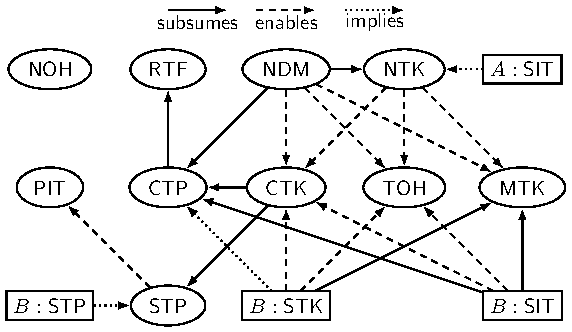
\includegraphics[scale = 0.7]{amass-dependency.pdf}
	\caption{Dependency graph for launch modes and intent flags in transitions $A \xrightarrow{\alpha(\phi)} B$. The launch modes %of $A$ and $B$ 
		(resp.\ the intent flags) are in boxes (resp. circles)}
		%in $\phi$
% \vspace{-6mm}	
	\label{fig-asm-depend}
\end{figure}


%%%%%%%%%%%%%%%%%%%%%%%%%%%%%%%%%%%%%%%%%%%%%%%
%%%%%%%%%%%%%%%%%%%%%%%%%%%%%%%%%%%%%%%%%%%%%%%
\hide{
\noindent\emph{\revision{understanding of the semantics}}

\revision{
For a given transition $A \xrightarrow{\startactivity(\phi)} B$.
Firstly, we consider two special cases, i.e., $\phi\models\tohflag$ and $\phi\models\mtkflag$, in these two cases, it need $\phi\models\ntkflag$.
\begin{itemize}
    \item If $\phi\models\tohflag$, it will clear up all the non-top tasks.
    \item If $\phi\models\mtkflag$, it will always launch a new task for $B$, except $\lmd(B) = \SIT/\STK$, since there is only one task with the real activity $B$ for the $\SIT$ or $\STK$ activity $B$.
\end{itemize}
Then we let $\phi\models\neg\tohflag\wedge\neg\mtkflag$, our semantics could be understood through the following mechanism:
\begin{enumerate}
    \item Determine which task will be associated with the caller activity $B$,
    \begin{itemize}
        \item If $\phi \models \ntkflag$ or if certain cases imply this, i.e., $\lmd(A) = \SIT$, $\lmd(B) = \SIT/\STK$, we need to specify a task that belongs to $B$ through the task allocation mechanism. If a task $S_i$ is found, then move the task $S_i$ to the top and proceed to step 2. Otherwise, launch a new task with $B$.
        \item Otherwise, proceed to step 2.
    \end{itemize}
    \item Determine how to place $B$ on top task, 
    \begin{itemize}
        \item If $\phi\models\neg\ctkflag\wedge\neg\ctpflag\wedge\neg\rtfflag$, then if the real activity of the top task or the top task is the main task, $B$ will be pushed into the top task.
        \item Otherwise $B$ is placed on the top task according to the dependencies between the launch mode of $B$ and the intent flags $\phi$. 
    \end{itemize}
\end{enumerate}
}
}
%%%%%%%%%%%%%%%%%%%%%%%%%%%%%%%%%%%%%%%%%%%%%%%
%%%%%%%%%%%%%%%%%%%%%%%%%%%%%%%%%%%%%%%%%%%%%%%


%Before describing the formal semantics, let us explain the intuition first.
%The system maintains fragment stack as well as transaction stack. 

%As mentioned in Section~\ref{sec:amm}, an activity %can be a plain activity meaning that it is unstructured and should be considered as atomic, or 
%contains sub-components 
%is structured and  in this paper we particularly focus on fragments. 
%Intuitively, %if 
%an activity contains a set of fragment containers each of which is associated with a \emph{fragment stack}, and features an \emph{transaction stack}. % to be used for defining the semantics of the action $\back$.)

%%%%%%%%%%%%%%%%%%%%%%%%%%%%%%%%%%%%%%%%%%%%%%%
%%%%%%%%%%%%%%%%%%%%%%%%%%%%%%%%%%%%%%%%%%%%%%%
\hide{
\subsection{Case $\tau = A \xrightarrow{\startactivity(\phi)} B$ and $\ell = 0$}
In this case, we distinguish two subcases, i.e., %Here we first assume that 
$\phi \models \neg \tohflag$ or $\phi \models \tohflag$. %We start with the first subcase. 

\subsection*{Case $\phi \models \neg \tohflag$}

%=================================================================================

\noindent {\fbox{$\lmd(B) = \singleinstance$}}
\begin{itemize}
	\item if $\getrealtsk(\rho, B) = S_i$ for some $i \in [n]$, 
        \begin{itemize}
            \item if $\phi\models\neg\ctkflag$, then $(\rho',\ell') = (\mvtsktop(\rho,i),0)$, $\jmath = (1,1)$ if $i = 1$, $\jmath = (2,1)$ otherwise,
            \item if $\phi\models\ctkflag$, then $(\rho',\ell') = (\clrtsk(\mvtsktop(\rho, i), B),\phi\models\nohflag)$, $\jmath = \bot$ if $i = 1$, $\jmath = (2,1)$ otherwise,
            % \item if $\phi\models\ctkflag\wedge\nohflag$, then $(\rho',\ell') = (\clrtsk(\mvtsktop(\rho, i), B),1)$, $\jmath = \bot$ if $i = 1$, $\jmath = (2,1)$ otherwise,
        \end{itemize}
	\item if $\getrealtsk(\rho, B) = *$, then $(\rho',\ell') = (\newtsk(\rho, B,\SIT),\phi\models\nohflag)$, $\jmath = (2,1)$.
	% \begin{itemize}
	% 	\item if $\phi\models\neg\nohflag$, then $(\rho',\ell') = (\newtsk(\rho, B),0)$,
	% 	\item if $\phi\models\nohflag$, then $(\rho',\ell') = (\newtsk(\rho, B),1)$.
	% \end{itemize}
\end{itemize}

\noindent {\fbox{$\lmd(B) = \singletask$}}
\begin{itemize}
	\item if $\getrealtsk(\rho, B) = S_i$ 
	or $ \getrealtsk(\rho, B) = * \wedge \gettsk(\rho, B) = S_i$, 
	\begin{itemize}
		\item if $\phi \models \neg \ctkflag $, 
		\begin{itemize}
			\item if $B \not \in S_i$, then $(\rho',\ell') = (\push(\mvtsktop(\rho,i),B),\phi\models\nohflag)$, $\jmath = (1,2)$ if $i = 1$, $\jmath = (2,1)$ otherwise,
			\item if $B \in S_i$, 	
			\begin{itemize}
				\item if $i = 1$ and $B = \topact(S_i)$, then $(\rho',\ell') = (\rho,0)$, $\jmath = (1,1)$,
				\item if $i = 1$ and $B \neq \topact(S_i)$, then $(\rho',\ell') = (\rho,0)$, $\jmath = \bot$,
				\item if $i \neq 1$, then $(\rho',\ell') = (\clrtop(\mvtsktop(\rho,i),B), 0)$, $\jmath = (2,1)$,
			\end{itemize}
		\end{itemize}
		\item if $\phi \models \ctkflag$, then $(\rho',\ell') = (\clrtsk(\mvtsktop(\rho, i), B),\phi\models\nohflag)$, $\jmath = \bot$ if $i = 1$, $\jmath = (2,1)$ otherwise,
	\end{itemize}
\item if $\gettsk(\rho, B) = *$, then $(\rho',\ell') = (\newtsk(\rho, B, \ntkflag),\phi\models\nohflag)$, $\jmath = (2,1)$.
\end{itemize}

\noindent {\fbox{$\lmd(B) = \standard$}}
\begin{itemize}
	\item if $\lmd(A) \neq \singleinstance$ and $\phi \models \neg \ntkflag$, 
	\begin{itemize}
        \item if $\phi\models\stpflag$ and $\topact(\rho) = B$, or $\phi\models\stpflag\wedge\pitflag$ and $\preact(\rho) = B$ , then $(\rho',\ell')=(\rho,0)$, $\jmath = (1,1)$,
        \item if $\phi\models\neg\stpflag\wedge\neg\rtfflag\wedge\neg\ctpflag$,
            or $\phi\models\stpflag\wedge\neg\rtfflag\wedge\neg\ctpflag$ and $B\neq\topact(\rho)$,
            or $\phi\models\stpflag\wedge\pitflag\wedge\neg\rtfflag\wedge\neg\ctpflag$ and $B\neq\preact(\rho)$,
            or $B\notin\toptsk(\rho)$,
                then $(\rho',\ell')=(\push(\rho, B),\phi\models\nohflag)$, $\jmath = (1,2)$,
        \item if $\phi \models \rtfflag \wedge \neg \ctpflag$ and $B \in \toptsk(\rho)$, then
         $(\rho',\ell')=(\mvacttop(\rho, B),0)$, $\jmath = (1,1)$ if $B = \topact(\rho)$, $\jmath = (1,2)$ otherwise,
        \item if $\phi \models\ctpflag\wedge\neg\stpflag$ and $B \in \toptsk(\rho)$, then
        $(\rho',\ell') =(\clrtop^*(\rho, B),\phi\models\nohflag)$, $\jmath = \bot$,
        \item if $\phi \models\ctpflag\wedge\stpflag$ and $B \in \toptsk(\rho)$, then
        $(\rho',\ell') =(\clrtop(\rho, B),0)$, $\jmath = (1,1)$ if $B = \topact(\rho)$, $\jmath = \bot$ otherwise,
	\end{itemize}
	\item if $\phi \models \ntkflag\wedge  \mtkflag\wedge\neg\ndmflag$, or $\lmd(A) = \singleinstance$ and $\phi \models \mtkflag\wedge\neg\ndmflag$,  then $(\rho',\ell') = (\newtsk(\rho, B, \ntkflag),\phi\models\nohflag)$, $\jmath = (2,1)$,
	\item if $\phi \models \ndmflag\wedge  \mtkflag$, then $(\rho',\ell') = (\newtsk(\rho, B, \ndmflag),\phi\models\nohflag)$, $\jmath = (2,1)$,
	\item if $\phi \models \ndmflag\wedge\neg\mtkflag$, 
    \begin{itemize}
        \item if $\getrealtsk(\rho,B) = S_i$, 
        \begin{itemize}
            \item if $\phi\models\neg\ctkflag$, then $(\rho',\ell')=(\clrtop(\mvtsktop(\rho,i), B),0)$, 
			\begin{itemize}
				\item if $i = 1$ and $B = \topact(\rho)$, then $\jmath = (1,1)$,
				\item if $i = 1$ and $B \neq \topact(\rho)$, then $\jmath = \bot$,
				\item if $i \neq 1$, then $\jmath = (2,1)$,
			\end{itemize}
            \item if $\phi\models\ctkflag$, then $(\rho',\ell') = (\clrtsk(\mvtsktop(\rho,i),B),\phi\models\nohflag)$, $\jmath = \bot$ if $i = 1$, $\jmath = (2,1)$ otherwise,
        \end{itemize}
        \item if $\getrealtsk(\rho,B) = *$, then $(\rho',\ell') = (\newtsk(\rho, B, \ndmflag),\phi\models\nohflag)$, $\jmath = (2,1)$,
    \end{itemize}
	%
	\item if $\phi \models \ntkflag\wedge \neg\ndmflag\wedge \neg \mtkflag$, or $\lmd(A) = \singleinstance$ and $\phi  \models \neg\ndmflag\wedge \neg \mtkflag$, then
	\begin{itemize}
        \item if $\getrealtsk(\rho, B) = S_i$ and $\zeta_i\neq\mainflag$,
            \begin{itemize}
            \item if $\phi\models\neg\ctkflag$ and $\topact(S_i) = B$, 
                or $\phi\models\neg\rtfflag\wedge\neg\ctpflag\wedge\neg\ctkflag$,
                then $(\rho',\ell')=(\mvtsktop(\rho, i), 0)$, $\jmath = (1,1)$ if $i = 1$, $\jmath = (2,1)$ otherwise,
            \item if $\phi\models(\rtfflag\vee\ctpflag)\wedge\neg\ctkflag$ and $B\notin S_i$,
				then $(\rho',\ell')=(\push(\mvtsktop(\rho, i), B),\phi\models\nohflag)$, $\jmath = (1,2)$ if $i = 1$, $\jmath = (2,1)$ otherwise,
            \item if $\phi \models \rtfflag \wedge \neg \ctpflag\wedge\neg\ctkflag$ and $B \in S_i$,
			then $(\rho',\ell')=(\mvacttop(\mvtsktop(\rho, i), B),0)$,
			\begin{itemize}
				\item if $i = 1$ and $B = \topact(\rho)$, then $\jmath = (1,1)$,
				\item if $i = 1$ and $B \neq \topact(\rho)$, then $\jmath = (1,2)$,
				\item if $i \neq 1$, then $\jmath = (2,1)$,
			\end{itemize}
            \item if $\phi \models\ctpflag\wedge\neg\stpflag\wedge\neg\ctkflag$ and $B \in S_i$, then $(\rho',\ell') =(\clrtop^*(\mvtsktop(\rho, i), B), \phi\models\nohflag)$, $\jmath = \bot$ if $i = 1$, $\jmath = (2,1)$ otherwise,
            \item if $\phi \models\ctpflag\wedge\stpflag\wedge\neg\ctkflag$ and $B \in S_i$, 
			then $(\rho',\ell') =(\clrtop(\mvtsktop(\rho, i), B), 0)$, 
			\begin{itemize}
				\item if $i = 1$ and $B = \topact(\rho)$, then $\jmath = (1,1)$,
				\item if $i = 1$ and $B \neq \topact(\rho)$, then $\jmath = \bot$,
				\item if $i \neq 1$, then $\jmath = (2,1)$,
			\end{itemize}
            \item if $\phi \models\ctkflag$, then
            $(\rho',\ell') = (\clrtsk(\mvtsktop(\rho, i), B),\phi\models\nohflag)$, $\jmath = \bot$ if $i = 1$, $\jmath = (2,1)$ otherwise,
            \end{itemize}
            \item if $\getrealtsk(\rho, B) = S_i$ and $\zeta_i=\mainflag$,
        or $ \getrealtsk(\rho, B) = * \wedge \gettsk(\rho, B) = S_i$, 
		\begin{itemize}
            \item if $\phi \models (\stpflag\vee\rtfflag\vee\ctpflag)\wedge\neg\ctkflag$ and $\topact(S_i) = B$,
            or $\phi \models \rtnflag \wedge\neg\rtfflag\wedge\neg\ctpflag\wedge\neg\ctkflag$,
			then $(\rho',\ell')=(\mvtsktop(\rho, i), 0)$, $\jmath = (1,1)$ if $i = 1$, $\jmath = (2,1)$ otherwise,
            \item if $\phi\models\neg\stpflag\wedge\neg\rtnflag\wedge\neg\rtfflag\wedge\neg\ctpflag\wedge\neg\ctkflag$,
                or $\phi\models\stpflag\wedge\neg\rtnflag\wedge\neg\rtfflag\wedge\neg\ctpflag\wedge\neg\ctkflag$ and $B\neq\topact(S_i)$,
                or $\phi\models\neg\rtnflag\wedge\neg\ctkflag$ and $B\notin S_i$,
				then $(\rho',\ell')=(\push(\mvtsktop(\rho, i), B),\phi\models\nohflag)$, $\jmath = (1,2)$ if $i = 1$, $\jmath = (2,1)$ otherwise,
            \item if $\phi \models \rtfflag \wedge \neg \ctpflag\wedge\neg\ctkflag$ and $B \in S_i$, 
			then $(\rho',\ell')=(\mvacttop(\mvtsktop(\rho, i), B),0)$,
			\begin{itemize}
				\item if $i = 1$ and $B = \topact(\rho)$, then $\jmath = (1,1)$,
				\item if $i = 1$ and $B \neq \topact(\rho)$, then $\jmath = (1,2)$,
				\item if $i \neq 1$, then $\jmath = (2,1)$,
			\end{itemize}
            \item if $\phi \models\ctpflag\wedge\neg\stpflag\wedge\neg\ctkflag$ and $B \in S_i$, then $(\rho',\ell') =(\clrtop^*(\mvtsktop(\rho, i), B), \phi\models\nohflag)$, $\jmath = \bot$ if $i = 1$, $\jmath = (2,1)$ otherwise,
            \item if $\phi \models\ctpflag\wedge\stpflag\wedge\neg\ctkflag$ and $B \in S_i$, then $(\rho',\ell') =(\clrtop(\mvtsktop(\rho, i), B), 0)$, 
			\begin{itemize}
				\item if $i = 1$ and $B = \topact(\rho)$, then $\jmath = (1,1)$,
				\item if $i = 1$ and $B \neq \topact(\rho)$, then $\jmath = \bot$,
				\item if $i \neq 1$, then $\jmath = (2,1)$,
			\end{itemize}
            \item if $\phi \models\ctkflag$, then
            $(\rho',\ell') = (\clrtsk(\mvtsktop(\rho, i), B),\phi\models\nohflag)$, $\jmath = \bot$ if $i = 1$, $\jmath = (2,1)$ otherwise,
		\end{itemize}
		\item if $\gettsk(\rho, B) = *$, then $(\rho',\ell') = (\newtsk(\rho, B, \ntkflag), \phi\models\nohflag)$, $\jmath = (2,1)$.
	\end{itemize}
\end{itemize}

\noindent  {\fbox{$\lmd(B) = \singletop$}}
\begin{itemize}
	\item if $\lmd(A) \neq \singleinstance$ and $\phi \models \neg \ntkflag\wedge\neg\ndmflag$, 
	\begin{itemize}
		\item if $\topact(\rho) = B$, or $\phi\models\pitflag$ and $\preact(\rho) = B$, then $(\rho',\ell')= (\rho,0)$, $\jmath = (1,1)$,
        \item if $\phi \models  \neg \rtfflag\wedge \neg \ctpflag$, and $B\neq\topact(\rho)$,
        or $\phi \models \pitflag\wedge\neg \rtfflag\wedge \neg \ctpflag$, and $B\neq\preact(\rho)$,
        or $B\notin \toptsk(\rho)$, then $(\rho',\ell')=(\push(\rho, B),\phi\models\nohflag)$, $\jmath = (1,2)$,
        %
        \item if $\phi \models \rtfflag \wedge \neg \ctpflag$ and $B \in \toptsk(\rho)$, then
         $(\rho',\ell')=(\mvacttop(\rho, B),0)$, $\jmath = (1,1)$ if $B = \topact(\rho)$, $\jmath = (1,2)$ otherwise,
        \item if $\phi \models\ctpflag$ and $B \in \toptsk(\rho)$, then
        $(\rho',\ell') =(\clrtop(\rho, B),0)$, $\jmath = (1,1)$ if $B = \topact(\rho)$, $\jmath = \bot$ otherwise,
	\end{itemize}
	\item if $\phi \models \ntkflag\wedge  \mtkflag\wedge\neg\ndmflag$, or $\lmd(A) = \singleinstance$ and $\phi \models \mtkflag\wedge\neg\ndmflag$,  then $(\rho',\ell') = (\newtsk(\rho, B, \ntkflag),\phi\models\nohflag)$, $\jmath = (2,1)$,
	\item if $\phi \models \ndmflag\wedge  \mtkflag$, then $(\rho',\ell') = (\newtsk(\rho, B, \ndmflag),\phi\models\nohflag)$, $\jmath = (2,1)$,
	\item if $\phi \models \ndmflag\wedge\neg\mtkflag$, 
    \begin{itemize}
        \item if $\getrealtsk(\rho,B) = S_i$, 
        \begin{itemize}
            \item if $\phi\models\neg\ctkflag$, then $(\rho',\ell')=(\clrtop(\mvtsktop(\rho,i), B),0)$, 
			\begin{itemize}
				\item if $i = 1$ and $B = \topact(\rho)$, then $\jmath = (1,1)$,
				\item if $i = 1$ and $B \neq \topact(\rho)$, then $\jmath = \bot$,
				\item if $i \neq 1$, then $\jmath = (2,1)$,
			\end{itemize}
            \item if $\phi\models\ctkflag$, then $(\rho',\ell') = (\clrtsk(\mvtsktop(\rho,i),B),\nohflag)$, $\jmath = \bot$ if $i = 1$, $\jmath = (2,1)$ otherwise,
        \end{itemize}
        \item if $\getrealtsk(\rho,B) = *$, then $(\rho',\ell') = (\newtsk(\rho, B, \ndmflag),\phi\models\nohflag)$, $\jmath = (2,1)$,
    \end{itemize}
	%
	\item if $\phi \models \ntkflag\wedge\neg\ndmflag\wedge \neg \mtkflag$, or $\lmd(A) = \singleinstance$ and $\phi  \models\neg\ndmflag\wedge \neg \mtkflag$, then
	\begin{itemize}
        \item if $\getrealtsk(\rho, B) = S_i$ and $\zeta_i\neq\mainflag$,
            \begin{itemize}
            \item if $\phi\models\neg\ctkflag$ and $\topact(S_i) = B$, 
                or $\phi\models\neg\rtfflag\wedge\neg\ctpflag\wedge\neg\ctkflag$,
                then $(\rho',\ell')=(\mvtsktop(\rho, i), 0)$, $\jmath = (1,1)$ if $i = 1$, $\jmath = (2,1)$ otherwise,
            \item if $\phi\models(\rtfflag\vee\ctpflag)\wedge\neg\ctkflag$ and $B\notin S_i$, 
				then $(\rho',\ell')=(\push(\mvtsktop(\rho, i), B),\phi\models\nohflag)$, $\jmath = (1,2)$ if $i = 1$, $\jmath = (2,1)$ otherwise,
            \item if $\phi \models \rtfflag \wedge \neg \ctpflag\wedge\neg\ctkflag$ and $B \in S_i$,
			then $(\rho',\ell')=(\mvacttop(\mvtsktop(\rho, i), B),0)$,
			\begin{itemize}
				\item if $i = 1$ and $B = \topact(\rho)$, then $\jmath = (1,1)$,
				\item if $i = 1$ and $B \neq \topact(\rho)$, then $\jmath = (1,2)$,
				\item if $i \neq 1$, then $\jmath = (2,1)$,
			\end{itemize}
            \item if $\phi \models\ctpflag\wedge\neg\ctkflag$ and $B \in S_i$, 
			then $(\rho',\ell') =(\clrtop(\mvtsktop(\rho, i), B), 0)$, 
			\begin{itemize}
				\item if $i = 1$ and $B = \topact(\rho)$, then $\jmath = (1,1)$,
				\item if $i = 1$ and $B \neq \topact(\rho)$, then $\jmath = \bot$,
				\item if $i \neq 1$, then $\jmath = (2,1)$,
			\end{itemize}
            \item if $\phi \models\ctkflag$, 
			then $(\rho',\ell') = (\clrtsk(\mvtsktop(\rho, i), B),\phi\models\nohflag)$, $\jmath = \bot$ if $i = 1$, $\jmath = (2,1)$ otherwise,
            \end{itemize}
            \item if $\getrealtsk(\rho, B) = S_i$ and $\zeta_i=\mainflag$,
        or $ \getrealtsk(\rho, B) = * \wedge \gettsk(\rho, B) = S_i$, 
		\begin{itemize}
            \item if $\phi \models \neg\ctkflag$ and $\topact(S_i) = B$, 
            or $\phi\models\rtnflag\wedge\neg\rtfflag\wedge\neg\ctpflag\wedge\neg\ctkflag$,
			then $(\rho',\ell')=(\mvtsktop(\rho, i), 0)$, $\jmath = (1,1)$ if $i = 1$, $\jmath = (2,1)$ otherwise,
            \item if $\phi\models\neg\rtnflag\wedge\neg\rtfflag\wedge\neg\ctpflag\wedge\neg\ctkflag$ and $B\neq\topact(S_i)$,
			or $\phi\models\neg\rtnflag\wedge\neg\ctkflag$ and $B\notin S_i$,
			then $(\rho',\ell')=(\push(\mvtsktop(\rho, i), B),\phi\models\nohflag)$, $\jmath = (1,2)$ if $i = 1$, $\jmath = (2,1)$ otherwise,
            \item if $\phi \models \rtfflag \wedge \neg \ctpflag\wedge\neg\ctkflag$ and $B \in S_i$, then 
			then $(\rho',\ell')=(\mvacttop(\mvtsktop(\rho, i), B),0)$,
			\begin{itemize}
				\item if $i = 1$ and $B = \topact(\rho)$, then $\jmath = (1,1)$,
				\item if $i = 1$ and $B \neq \topact(\rho)$, then $\jmath = (1,2)$,
				\item if $i \neq 1$, then $\jmath = (2,1)$,
			\end{itemize}
            \item if $\phi \models\ctpflag\wedge\neg\ctkflag$ and $B \in S_i$, 
			then $(\rho',\ell') =(\clrtop(\mvtsktop(\rho, i), B), 0)$, 
			\begin{itemize}
				\item if $i = 1$ and $B = \topact(\rho)$, then $\jmath = (1,1)$,
				\item if $i = 1$ and $B \neq \topact(\rho)$, then $\jmath = \bot$,
				\item if $i \neq 1$, then $\jmath = (2,1)$,
			\end{itemize}
            \item if $\phi \models\ctkflag$,
			then $(\rho',\ell') = (\clrtsk(\mvtsktop(\rho, i), B),\phi\models\nohflag)$, $\jmath = \bot$ if $i = 1$, $\jmath = (2,1)$ otherwise,
		\end{itemize}
		\item if $\gettsk(\rho, B) = *$, then $(\rho',\ell') = (\newtsk(\rho, B, \ntkflag), \phi\models\nohflag)$, $\jmath = (2,1)$.
	\end{itemize}
	
\end{itemize}


%%%%%%%%%%%%%%%%%%%%%%%%%%%%%%%%%%%%%%%%%%%%%%%%%%%%%%%%%%%%%%%%%%%%%%%%%%%%%%%%%%%%%%%%%%%%%%%%%%%
\subsection*{Case $\phi \models \tohflag$}
%
We then consider the transition rules $\tau =A \xrightarrow{\startactivity(\phi)} B$ with $\phi \models \tohflag\wedge(\ntkflag\vee\ndmflag)$, 
or $\lmd(A) = \singleinstance$ and $\phi\models\tohflag$,
or $\lmd(B) = \singleinstance/\singletask$ and $\phi\models\tohflag$. It turns out that we can largely reuse the semantic definitions of the case that $\phi \models \neg \tohflag$. Namely, 
let $\tau' = A \xrightarrow{\startactivity(\phi')} B$ where $\phi'$ is obtained from $\phi$ by replacing $\tohflag$ with $\neg \tohflag$. (The behavior of $\tau'$ is fully prescribed before, viz, $(\rho,\ell) \xrightarrow[\tau',\jmath']{\Mm} (\rho',\ell')$ where $\rho' = ((S'_1, A'_1,\zeta'_1), \cdots, (S'_{n'}, A'_{n'},\zeta'_{n'}))$. Then we have that $(\rho,\ell) \xrightarrow[\tau,\jmath]{\Mm} ((S'_1, A'_1,\zeta'_1))$ and $\jmath = \bot$ if $\jmath' = (2,1)$, $\jmath = \jmath'$ otherwise.

%\smallskip
%\noindent \fbox{Case $\tau = A \xrightarrow{\finishstart(\phi)} B$}
%\smallskip
\subsection{Case $\tau = A \xrightarrow{\finishstart(\phi)} B$}

In this case, $A\xrightarrow {\finishstart(\phi)}B$ specifies that $B$ is started with the intent flags $\phi$ followed by the termination of $A$, popped from the task stack. Let
%Suppose that $\rho$ is the current configuration with 
%$\rho=((S_1,A_1,b_1), \cdots, (S_n, A_n, b_n))$, let $S_1=[A]\cdot S_1'$, where $S_1'\in\act^*$.
$\tau' = A \xrightarrow {\startactivity(\phi)}B$ and $(\rho,0) \xrightarrow[\tau',\jmath]{\Mm} (\rho'',\ell'')$, then we have $(\rho,\ell) \xrightarrow[\tau,\jmath]{\Mm} (\rho',\ell'')$, where $\rho = \rmact(\rho'', x, y)$ if $\jmath = (x, y)$, $\rho' = \rho''$ otherwise.

\subsection{Case $\tau = A \xrightarrow{\alpha(\phi)} B$ and $\ell = 1$}

Similarly, it specifies that $B$ is started with the intent flags $\phi$ followed by the termination of $A$, popped from the task stack. Let
$(\rho,0) \xrightarrow[\tau,\jmath]{\Mm} (\rho'',\ell'')$, then we have $(\rho,1) \xrightarrow[\tau,\jmath]{\Mm} (\rho',\ell'')$, where $\rho = \rmact(\rho'', x, y)$ if $\jmath = (x, y)$, $\rho' = \rho''$ otherwise.

%then $\rho \xrightarrow[\tau]{\Mm} \rho'$, where $\rho''\xrightarrow[\tau']{\Mm}\rho'$ and $\rho''$ is defined as follows:
%\begin{itemize}
%    \item if $|S_1'|>0$, then $\rho''=( (S_1',A_1,b_1)\cdots,(S_n,A_n,b_n) )$,
%    \item otherwise, $\rho''=( (S_2,A_2,b_2)\cdots,(S_n,A_n,b_n) )$.
%\end{itemize}
%Then we have $\rho \xrightarrow[\tau]{\Mm} \rho'$.

%Proposition~\ref{prop:sem} reassures that $\xrightarrow{\Aa}$ is indeed a relation on $\conf_\Aa$ as per Definition~\ref{def-ass-conf}.
%
%\begin{proposition} \label{prop:sem}
%	Let $\Aa$ be an ASM. For each $(q, \rho) \in \conf_\Aa$ and  $(q, \rho) \xrightarrow{\Aa} (q', \rho')$,
%	$(q', \rho') \in \conf_\Aa$, namely, $(q', \rho')$  satisfies the five constraints in Definition~\ref{def-ass-conf}.
%\end{proposition}


%\noindent\hlfancyfancy{$\mathcolorbox{highlightcolor}{\mbox{Case }\tau = A \xrightarrow{\opstack} (\beta_1(F_1, i_1), \cdots, \beta_k(F_k, i_k))}$}
%\noindent\fbox{Case $\tau = A \xrightarrow{\opstack} (\beta_1(F_1, i_1), \cdots, \beta_k(F_k, i_k))$}
%\smallskip


\subsection{Case $\tau = A \xrightarrow{\opstack} (\beta_1(F_1, i_1, x_1), \cdots, \beta_k(F_k, i_k, x_k))$}\ 

%Suppose $S_1 = [(B_1, \Theta_1), \cdots, (B_r, \Theta_r)]$ (where $B_1 = A$ and $\Theta_1 = \Theta$). 
In this case, 
let $T = (\beta_1(F_1, i_1, x_1), \cdots, \beta_k(F_k, i_k, x_k))$. 
Then we have $(\rho,\ell) \xrightarrow[\tau,(1,1)]{\Mm} (\rho',\ell)$, where
%$i=1$, $\ell' = \ell$, and 
$$\rho' = ((S'_1, A_1,\zeta_1), (S_2, A_2,\zeta_2), \cdots, (S_n, A_n,\zeta_n))$$ is obtained from $\rho$ by applying all the actions in $T$ to the containers and assignment function in $\Theta=\Theta_1$ (recall that $\tact(S_1) = (A, \Theta)$), specifically,  
$S'_1 =[(B_1, \Theta'_1), (B_2, \Theta_2), \cdots, (B_r, \Theta_r)],$ 
where $\Theta'_1 = (\upsilon', \eta', \iota')$ such that $(\upsilon', \iota') = \updateviews_{T}(\upsilon, \iota)$ and $\eta' = \concaction_{\upsilon, \iota}(T) \cdot \eta$.

%\smallskip 
%\noindent\fbox{Case $\tau = A \xrightarrow{\nopstack} (\beta_1(F_1, i_1), \cdots, \beta_k(F_k, i_k))$}
%\smallskip
 
%Suppose $S_1 = [(B_1, \Theta_1), \cdots, (B_r, \Theta_r)]$ (where $B_1 = A$ and $\Theta_1 = \Theta$). 

\subsection{Case $\tau = A \xrightarrow{\nopstack} (\beta_1(F_1, i_1, x_1), \cdots, \beta_k(F_k, i_k, x_k))$}\ 

In this case, let $T = (\beta_1(F_1, i_1, x_1), \cdots, \beta_k(F_k, i_k, x_k))$,
Then we have $(\rho,\ell) \xrightarrow[\tau,(1,1)]{\Mm} (\rho',\ell)$, where
$$\rho' = ((S'_1, A_1,\zeta_1), (S_2, A_2,\zeta_2), \cdots, (S_n, A_n,\zeta_n))$$ such that 
$$S'_1 =[(B_1, \Theta'_1), (B_2, \Theta_2), \cdots, (B_r, \Theta_r)],$$ 
where $\Theta'_1 = (\upsilon', \eta, \iota')$, and $(\upsilon', \iota') = \updateviews_{T}(\upsilon, \iota)$. Note that in this case, the concretization of $T$ is not stored into the transaction stack. 

%\smallskip
%\noindent \fbox{Case $\tau = \back$}
%\smallskip

\subsection{Case $\tau = \back$}
In this case, we distinguish two subcases, i.e., $\eta=\epsilon$ or $\eta\neq\epsilon$.
\subsection*{Case $\eta=\epsilon$}
In this case, if $S_1$ contains exactly one activity (i.e. $A$), then $S_1$ disappears after the $\back$ action, that is, $(\rho,\ell) \xrightarrow[\tau,\bot]{\Mm} (\rho',0)$, where $\rho' = ((S_2, A_2,\zeta_2), \cdots, (S_n, A_n,\zeta_n))$.
On the other hand, if $S_1$ contains at least two activities, then $(\rho,\ell) \xrightarrow[\tau,\bot]{\Mm} (\rho',0)$, where $\rho' = ((S'_1,A_1,\zeta_1), (S_2, A_2,\zeta_2), \cdots, (S_n, A_n,\zeta_n))$ and $S'_1$ is obtained from $S_1$ by removing the top activity $A$ from $S_1$.
\subsection*{Case $\eta\neq\epsilon$}
In this case, 
$(\rho,\ell) \xrightarrow[\tau,(1,1)]{\Mm} (\rho',\ell)$, where %$i = 1$, $\ell' = \ell$, and 
$$\rho' = ((S'_1, A_1,\zeta_1), (S_2, A_2,\zeta_2), \cdots, (S_n, A_n,\zeta_n))$$
such that 
$$S'_1 =[(B_1, \Theta'_1), (B_2, \Theta_2), \cdots, (B_r, \Theta_r)],$$ 
where 
$\Theta'_1 = (\upsilon', \eta', \iota')$, $(\upsilon', \iota') = \updateviews_{T_1^{-1}}(\upsilon, \iota),$ and $\eta' = (T_2, \cdots, T_l)$.
Note that $T_1$ is popped off the transaction stack and the actions of $T_1$ are revoked on $(\upsilon, \iota)$.
 

%%%%%%%%%%%%%%%%%%%%%%%%%%%%%%%%%%%%%%%%%%
\subsection{Other cases}
When $\upsilon \neq (\epsilon, \cdots, \epsilon)$, the fragment stacks of $A$ contains at least one fragment and the transition rules of the following form are applicable, namely,  $F \xrightarrow{\startactivity(\phi)} B$, $ F \xrightarrow{\finishstart(\phi)} B$,  $F \xrightarrow{\opstack} (\beta_1(F_1, i_1, x_1), \cdots, \beta_k(F_k, i_k, x_k))$, and $F \xrightarrow{\nopstack} (\beta_1(F_1, i_1, x_1), \cdots, \beta_k(F_k, i_k, x_k))$  with $F \in \tfrag(\upsilon)$. 
The semantics of these rules are similar to those of the case of the source is activity.
}
%We will focus on the transition rules $\tau = F \xrightarrow{\mu} (\beta_1(F_1, i_1), \cdots, \beta_k(F_k, i_k))$ (where $\mu \in \{\opstack, \nopstack\}$) 
%$F \xrightarrow{\nopstack} (\beta_1(F_1, i_1), \cdots, \beta_k(F_k, i_k))$, 
%The semantics of the other rules are similar to those of the case $v=(\epsilon,\cdots,\epsilon)$ above.
%$A \xrightarrow{\mu} (\beta_1(F_1, i_1), \cdots, \beta_k(F_k, i_k))$ above.
\hide{
Suppose $S_1 = [(B_1, \Theta_1), \cdots, (B_r, \Theta_r)]$ (where $B_1 = A$ and $\Theta_1 = \Theta$). 
\smallskip
\noindent\fbox{Case $\tau = F \xrightarrow{\opstack} (\beta_1(F_1, i_1), \cdots, \beta_k(F_k, i_k))$}
 

%Suppose $S_1 = [(B_1, \Theta_1), \cdots, (B_r, \Theta_r)]$ (where $B_1 = A$ and $\Theta_1 = \Theta$). 

Let $T = (\beta_1(F_1, i_1), \cdots, \beta_k(F_k, i_k))$. 
In this case, $\rho \xrightarrow[\tau]{\Mm} \rho'$, where 
$$\rho' = ((S'_1, A_1,b_1), (S_2, A_2,b_2), \cdots, (S_n, A_n,b_n))$$
such that $S'_1 =[(B_1, \Theta'_1), (B_2, \Theta_2), \cdots, (B_r, \Theta_r)]$, $\Theta'_1 = (\upsilon', \eta')$, $\upsilon' = \updateviews^\sharp_{T}(\upsilon)$, and $\eta' = \concaction^\sharp_\upsilon(T) \cdot \eta$.

  \smallskip
\noindent\fbox{Case $\tau = F \xrightarrow{\nopstack} (\beta_1(F_1, i_1), \cdots, \beta_k(F_k, i_k))$}
 


%Suppose $S_1 = [(B_1, \Theta_1), \cdots, (B_r, \Theta_r)]$ (where $B_1 = A$ and $\Theta_1 = \Theta$). 

Let $T = (\beta_1(F_1, i_1), \cdots, \beta_k(F_k, i_k))$. 
In this case, $\rho \xrightarrow[\tau]{\Mm} \rho'$, where 
$$\rho' = ((S'_1, A_1,b_1), (S_2, A_2,b_2), \cdots, (S_n, A_n,b_n))$$
such that $S'_1 =[(B_1, \Theta'_1), (B_2, \Theta_2), \cdots, (B_r, \Theta_r)]$, $\Theta'_1 = (\upsilon', \eta)$, and $\upsilon' = \updateviews_{T}(\upsilon)$.
}
%%%%%%%%%%%%%%%%%%%%%%%%%%%%%%%%%%%%%%%%%%%%%%%
%%%%%%%%%%%%%%%%%%%%%%%%%%%%%%%%%%%%%%%%%%%%%%%


\section{Semantics of {\AMASS} models for the other versions of Android}
%
We state the differences of the semantics of {$\AMASS$} models in details. To avoid tediousness, let us focus on the situation $\phi \models \neg \tohflag$. The differences for the situation $\phi \models \tohflag$ are similar. 

\subsection{Android 11.0 and 12.0.}
The semantics of {\AMASS} for Android 11.0 and 12.0 are the same as Android 13.0. 

\subsection{Android 10.0, 9.0, and 8.0.}
The semantics for these three versions are the same and differ from that for Android 13.0 in the following sense: $\rtfflag$ is ignored when used together with $\ntkflag$ or $\lmd(A) = \SIT$. 
That is, for Android 10.0, 9.0, and 8.0, the semantics of $\AMASS$ for the case $\lmd(B) = \STD$ and $\phi \models \ntkflag \wedge \neg \ndmflag\wedge \neg \mtkflag$, or $\lmd(A) = \SIT$ and $\phi \models \neg\ndmflag\wedge\neg\mtkflag$, is adapted from Android 13.0 as follows.

%When $\phi \models \ntkflag \wedge \neg\ndmflag\wedge\neg \mtkflag$, $\rtfflag$ is ignored. 
%
\begin{itemize}
    \item if $\getrealtsk(\rho, B) = S_i$ or $\getrealtsk(\rho,B) = * \wedge\gettsk(\rho,B) = S_i$, then
    \begin{itemize}
    \item if $i \neq 1$, then 
        \begin{itemize}
            \item if $\phi \models \ctkflag$, then $\cdots$ 
            \item if $\phi \models \neg \ctkflag$, then $\cdots$
                \begin{itemize}
                    \item if $\phi \models\ctpflag$ and $B \in S_i$, then $\cdots$
                    \item if $\phi \models\ctpflag$ and $B \notin S_i$, then $\cdots$
                    \item if $\phi \models\neg\ctpflag$, then
                    \begin{itemize}
							\item if $\getrealtsk(\rho,B) = S_i$ and $\zeta_i \neq \mainflag$, then $b' = \neg \nohflag$, moreover,
							\begin{itemize}
								\item if $b = \neg \nohflag$ and $\alpha = \startactivity$, then $\rho'=\mvtsktop(\rho, i)$,
								\item otherwise, $\rho' = \rmact(\mvtsktop(\rho, i), 2, 1)$, 
							\end{itemize}
							\item otherwise ($\getrealtsk(\rho,B) = S_i$ and $\zeta_i = \mainflag$ or $\getrealtsk(\rho,B) = * \wedge\gettsk(\rho,B) = S_i$), 
							\begin{itemize}
								\item if $\phi\models\stpflag$ and $\topact(S_i) = B$, then $b' = \neg \nohflag$, moreover,
								\begin{itemize}
									\item if $b = \neg \nohflag$ and $\alpha = \startactivity$, then $\rho'=\mvtsktop(\rho, i)$,
									\item otherwise, $\rho' = \rmact(\mvtsktop(\rho, i), 2, 1)$, 
								\end{itemize}
								\item otherwise, $b' = \nohflag$ iff $\phi \models \nohflag$, moreover, 
								\begin{itemize}
									\item if $b = \neg \nohflag$ and $\alpha = \startactivity$, then $\rho'=\push(\mvtsktop(\rho, i), B)$,
									\item otherwise, $\rho' = \rmact(\push(\mvtsktop(\rho, i), B), 2, 1)$, 
								\end{itemize}
							\end{itemize}
                    \end{itemize}
                \end{itemize}
        \end{itemize}
    \item otherwise ($i  = 1$),  
    \begin{itemize}
        \item if $\phi \models \ctkflag$, then $\cdots$, 
        \item if $\phi \models \neg \ctkflag$, then 
        \begin{itemize}
            \item if $\phi \models \ctpflag$ and $B \in S_1$, then $\cdots$
%				\begin{itemize}
%					\item if $\phi\models \neg \stpflag$, then $b' = \nohflag$ iff $\phi \models \nohflag$, 
%					\item otherwise, $b' = \neg \nohflag$,
%				\end{itemize}
            \item if $\phi \models \ctpflag$ and $B\notin S_1$, then $\cdots$
            \item if $\phi \models \neg \ctpflag$, then
            \begin{itemize}
				\item if $\getrealtsk(\rho,B) = S_1$ and $\zeta_1 \neq \mainflag$, 
				\begin{itemize}
					\item if $\alpha = \startactivity$, then $\rho' = \rho$ and $b' = b$,
					\item if $\alpha = \finishstart$, then $\rho' = \rmact(\rho, 1, 1)$ and $b' = \neg\nohflag$,
				\end{itemize}
			\item otherwise ($\getrealtsk(\rho,B) = S_1$ and $\zeta_i = \mainflag$ or $\getrealtsk(\rho,B) = * \wedge\gettsk(\rho,B) = S_1$), 
			\begin{itemize}
				\item if $\phi\models\stpflag$ and $A = B$, or $\phi \models\stpflag\wedge\pitflag$ and $\preact(\rho) = B$, 
				\begin{itemize}
					\item if $\alpha = \startactivity$, then $\rho' = \rho$ and $b' = b$,
					\item if $\alpha = \finishstart$, then $\rho' = \rmact(\rho, 1, 1)$ and $b' = \neg\nohflag$,
				\end{itemize}
				\item otherwise, $b' = \nohflag$ iff $\phi \models \nohflag$, moreover, 
				\begin{itemize}
					\item if $b = \neg \nohflag$ and $\alpha = \startactivity$, then $\rho'=\push(\rho, B)$,
					\item otherwise, $\rho' = \rmact(\push(\rho, B), 1, 2)$, 
				\end{itemize}
			\end{itemize}
            \end{itemize}
        \end{itemize}
    \end{itemize}
\end{itemize}
\item if $\gettsk(\rho, B) = *$, then $\cdots$. 
\end{itemize}
Similarly the semantics of $\AMASS$ for the case $\lmd(B) = \STP$ and $\phi \models \ntkflag \wedge \neg \ndmflag\wedge \neg \mtkflag$ or $\lmd(A) = \SIT$ and $\phi \models \neg\ndmflag\wedge\neg\mtkflag$ is adapted from Android 13.0 as follows.

\begin{itemize}
    \item if $\getrealtsk(\rho, B) = S_i$ or $\getrealtsk(\rho,B) = * \wedge\gettsk(\rho,B) = S_i$, then
    \begin{itemize}
    \item if $i \neq 1$, then 
        \begin{itemize}
            \item if $\phi \models \ctkflag$, then $\cdots$ 
            \item if $\phi \models \neg \ctkflag$, then $\cdots$
                \begin{itemize}
                    \item if $\phi \models\ctpflag$ and $B \in S_i$, then $\cdots$
                    \item if $\phi \models\ctpflag$ and $B \notin S_i$, then $\cdots$
                    \item if $\phi \models\neg\ctpflag$, then
                    \begin{itemize}
							\item if $\getrealtsk(\rho,B) = S_i$ and $\zeta_i \neq \mainflag$, then $b' = \neg \nohflag$, moreover,
							\begin{itemize}
								\item if $b = \neg \nohflag$ and $\alpha = \startactivity$, then $\rho'=\mvtsktop(\rho, i)$,
								\item otherwise, $\rho' = \rmact(\mvtsktop(\rho, i), 2, 1)$, 
							\end{itemize}
							\item otherwise ($\getrealtsk(\rho,B) = S_i$ and $\zeta_i = \mainflag$ or $\getrealtsk(\rho,B) = * \wedge\gettsk(\rho,B) = S_i$), 
							\begin{itemize}
								\item if $\topact(S_i) = B$, then $b' = \neg \nohflag$, moreover,
								\begin{itemize}
									\item if $b = \neg \nohflag$ and $\alpha = \startactivity$, then $\rho'=\mvtsktop(\rho, i)$,
									\item otherwise, $\rho' = \rmact(\mvtsktop(\rho, i), 2, 1)$, 
								\end{itemize}
								\item otherwise, $b' = \nohflag$ iff $\phi \models \nohflag$, moreover, 
								\begin{itemize}
									\item if $b = \neg \nohflag$ and $\alpha = \startactivity$, then $\rho'=\push(\mvtsktop(\rho, i), B)$,
									\item otherwise, $\rho' = \rmact(\push(\mvtsktop(\rho, i), B), 2, 1)$, 
								\end{itemize}
							\end{itemize}
                    \end{itemize}
                \end{itemize}
        \end{itemize}
    \item otherwise ($i  = 1$),  
    \begin{itemize}
        \item if $\phi \models \ctkflag$, then $\cdots$, 
        \item if $\phi \models \neg \ctkflag$, then 
        \begin{itemize}
            \item if $\phi \models \ctpflag$ and $B \in S_1$, then $\cdots$
%				\begin{itemize}
%					\item if $\phi\models \neg \stpflag$, then $b' = \nohflag$ iff $\phi \models \nohflag$, 
%					\item otherwise, $b' = \neg \nohflag$,
%				\end{itemize}
            \item if $\phi \models \ctpflag$ and $B\notin S_1$, then $\cdots$
            \item if $\phi \models \neg \ctpflag$, then
            \begin{itemize}
				\item if $\getrealtsk(\rho,B) = S_1$ and $\zeta_1 \neq \mainflag$, 
				\begin{itemize}
					\item if $\alpha = \startactivity$, then $\rho' = \rho$ and $b' = b$,
					\item if $\alpha = \finishstart$, then $\rho' = \rmact(\rho, 1, 1)$ and $b' = \neg\nohflag$,
				\end{itemize}
			\item otherwise ($\getrealtsk(\rho,B) = S_1$ and $\zeta_i = \mainflag$ or $\getrealtsk(\rho,B) = * \wedge\gettsk(\rho,B) = S_1$), 
			\begin{itemize}
				\item if $A = B$, or $\phi \models\pitflag$ and $\preact(\rho) = B$, 
				\begin{itemize}
					\item if $\alpha = \startactivity$, then $\rho' = \rho$ and $b' = b$,
					\item if $\alpha = \finishstart$, then $\rho' = \rmact(\rho, 1, 1)$ and $b' = \neg\nohflag$,
				\end{itemize}
				\item otherwise, $b' = \nohflag$ iff $\phi \models \nohflag$, moreover, 
				\begin{itemize}
					\item if $b = \neg \nohflag$ and $\alpha = \startactivity$, then $\rho'=\push(\rho, B)$,
					\item otherwise, $\rho' = \rmact(\push(\rho, B), 1, 2)$, 
				\end{itemize}
			\end{itemize}
            \end{itemize}
        \end{itemize}
    \end{itemize}
\end{itemize}
\item if $\gettsk(\rho, B) = *$, then $\cdots$. 
\end{itemize}

Note that the parts of the semantics denoted by $\cdots$ are the same as Android 13.0, and in the semantics for the situation $\phi \models \neg \ctpflag$, the flag $\rtfflag$ has no effects, thus is ignored.  



%Moreover, the semantics in the case $\phi \models \tohflag$ should be similarly adapted for $\rtfflag$.

%$\rtfflag$ flag will be omitted when $\phi\models\ntkflag$ or $\lmd(A) = \singleinstance$ for $A\xrightarrow{\alpha(\phi)}B$. More precisely, the semantics can be adapted from that for Android 12.0 as follows:
%\begin{itemize}
%    \item for the subcase $\phi \models \ntkflag\wedge \neg \mtkflag$, or $\lmd(A) = \singleinstance$ and $\phi  \models \neg \mtkflag$ of the case $\lmd(B) = \standard$ and $\lmd(B) = \singletop$, 
 %       remove $\rtfflag$ in the formulae $\phi$, and remove the item which constraint is $\phi\models\rtfflag\wedge\neg\ctpflag\wedge\neg\ctkflag$ and $B\in S_j$.
%\end{itemize}

\subsection{Android 7.0.}
The semantics for Android 7.0 is close to that of Android 10.0 (or 9.0, 8.0) but differs from it in the following two aspects:  1) the effect of $\ndmflag$ is the same as that of $\ntkflag$, 2)
when $\phi \models \neg \ntkflag \wedge \neg\ndmflag \wedge \neg\ctpflag$, if the top task is the main task where the started activity occurs but is not the top activity, then $\rtfflag$ has the same effect as $\ctkflag$. More precisely, for Android 7.0, only two cases ``$\phi \models \ntkflag$ or $\lmd(A) = \SIT$'' and ``$\phi  \models \neg \ntkflag$ and $\lmd(A)\neq\SIT$'' are considered, where the semantics for the case ``$\phi \models \ntkflag$ or $\lmd(A) = \SIT$'' inherits that of ``$\phi \models \ntkflag \wedge \neg \ndmflag$ or $\lmd(A) = \SIT$ and $\phi\models\neg\ndmflag$'' for Android 10.0, while the semantics for the case ``$\phi  \models \neg \ntkflag$ and $\lmd(A) \neq \SIT$'' is adapted from that of ``$\phi \models \neg \ntkflag \wedge \neg \ndmflag$ and $\lmd(A) \neq \SIT$'' for Android 10.0 as follows. 
%
%
%        \item if $\phi \models \rtfflag \wedge \neg \ctpflag$ and $B \in \toptsk(\rho)$, then
 %        $\rho'=\mvacttop(\rho, B)$,
%
\begin{itemize}
	\item If $\phi \models \ctpflag$ and $B \in \toptsk(\rho)$, then $\cdots$.
	\item If $\phi \models \ctpflag$ and $B \not \in \toptsk(\rho)$, then $\cdots$.
	\item If $\phi \models \neg \ctpflag$, then
		\begin{itemize}
    			\item if $\phi \models \rtfflag$ and $B \in \toptsk(\rho)$, then
    			\begin{itemize}
        				\item if $\topact(\rho) \neq B$, then $b' = \neg \nohflag$, moreover, 
       	 			\begin{itemize}
            				\item if $\zeta_i = \mainflag$, then $\rho' = \clrtsk(\rho, B)$,
            				\item otherwise,
            				\begin{itemize}
                					\item if $b = \neg \nohflag$ and $\alpha = \startactivity$, then $\rho'= \mvacttop(\rho, B)$, 
                					\item otherwise, $\rho' = \rmact(\mvacttop(\rho, B), 1, 2)$, 
            				\end{itemize}
        				\end{itemize}
        				\item if $\topact(\rho) = B$, 
						\begin{itemize}
							\item if $\alpha = \startactivity$, then $\rho' = \rho$ and $b' = b$,
							\item if $\alpha = \finishstart$, then $\rho' = \rmact(\rho, 1, 1)$ and $b' = \neg\nohflag$,
						\end{itemize}
    			\end{itemize}
			\item if $\phi \models \rtfflag$ and $B \not \in \toptsk(\rho)$, then $\cdots$,
			\item if $\phi \models \neg \rtfflag$, then $\cdots$.
		\end{itemize}
\end{itemize}
%Intuitively, when $\phi \models \rtfflag \wedge \neg \ctpflag$, $B \in \toptsk(\rho)$, and additionally the top task is the main task, the top task is cleared before pushing $B$.

%$\ndmflag$ has the same effects with $\ntkflag$, and for each item $\ndmflag$ and $\neg\ndmflag$ are removed.

%In Android 7.0, $\rtfflag$ flag will clear the task when the current task is the main task. More precisely, the semantics of Android 7.0 is defined as follows.
%\begin{itemize}
%    \item for the subcase $\lmd(A) \neq \singleinstance$ and $\phi \models \neg \ntkflag$ of the case $\lmd(B) = \standard$ and $\lmd(B) = \singletop$, replace the constraint with $\phi\models\rtfflag\wedge\neg\ctpflag$ and $B\in S_j$ and $b_1=0$,
%        of the item which constraint is $\phi\models\rtfflag\wedge\neg\ctpflag$ and $B\in S_j$,
%        and add an item: if $\phi\models\rtfflag\wedge\neg\ctpflag$ and $B\in S_j$ and $b_1=1$,
%        then $\rho' = \push(\clrtsk(\rho),B)$.
%\end{itemize}

\subsection{Android 6.0.}
The semantics for Android 6.0 differs from that of Android 10.0 (or 9.0, 8.0) in the following two aspects: 1) the effect of $\ndmflag$ is the same as that of $\ntkflag$, 2) the task allocation mechanism of Android 6.0 does not use the real activities of tasks and only relies on affinities. 
%
More precisely, for Android 6.0, only two cases ``$\phi \models \ntkflag$ or $\lmd(A) = \SIT$'' and ``$\phi  \models \neg \ntkflag$ and $\lmd(A)\neq\SIT$'' are considered, where the semantics for the case ``$\phi \models \ntkflag$ or $\lmd(A) = \SIT$'' inherits that of ``$\phi \models \ntkflag \wedge \neg \ndmflag$ or $\lmd(A) = \SIT$ and $\phi\models\neg\ndmflag$'' for Android 10.0, while the semantics for the case ``$\phi  \models \ntkflag$ or $\lmd(A) = \SIT$ and $\phi\models\neg\mtkflag$'' is adapted from that of ``$\phi \models \ntkflag \wedge \neg \ndmflag\wedge\neg\mtkflag$ or $\lmd(A) = \SIT$ and $\phi\models\neg\ndmflag\wedge\mtkflag$'' for the case $\lmd(B) = \STD$ for Android 10.0 as follows, where the conditions involving $\getrealtsk(\rho, B)$ and $\gettsk(\rho, B)$ are simplified into the conditions involving only $\gettsk(\rho, B)$, moreover, we do not need to distinguish whether a task is the main task or not.  
\begin{itemize}
    \item if $\gettsk(\rho,B) = S_i$, then
%    // {\it $\getrealtsk(\rho, B) = S_i$ or $\getrealtsk(\rho,B) = * \wedge\gettsk(\rho,B) = S_i$ is replaced by $\gettsk(\rho,B) = S_i$}
    \begin{itemize}
    \item if $i \neq 1$, then 
        \begin{itemize}
            \item if $\phi \models \ctkflag$, then $\cdots$ 
            \item if $\phi \models \neg \ctkflag$, then $\cdots$
                \begin{itemize}
                    \item if $\phi \models\ctpflag$ and $B \in S_i$, then $\cdots$
                    \item if $\phi \models\ctpflag$ and $B \notin S_i$, then $\cdots$
                    \item if $\phi \models\neg\ctpflag$, then
%                    \begin{itemize}
%                            \item if $\getrealtsk(\rho,B) = S_i$ and $\zeta_i \neq \mainflag$, then $b' = \neg \nohflag$, moreover,
%                            \begin{itemize}
%                                \item if $b = \neg \nohflag$, then $\rho'=\mvtsktop(\rho, i)$,
%                                \item otherwise, $\rho' = \rmact(\mvtsktop(\rho, i), 2, 1)$, 
%                            \end{itemize}
%                            \item otherwise ($\getrealtsk(\rho,B) = S_i$ and $\zeta_i = \mainflag$ or $\getrealtsk(\rho,B) = * \wedge\gettsk(\rho,B) = S_i$), 
                            \begin{itemize}
                                \item if $\phi\models\stpflag$ and $\topact(S_i) = B$, then $b' = \neg \nohflag$, moreover,
                                \begin{itemize}
                                    \item if $b = \neg \nohflag$ and $\alpha = \startactivity$, then $\rho'=\mvtsktop(\rho, i)$,
                                    \item otherwise, $\rho' = \rmact(\mvtsktop(\rho, i), 2, 1)$, 
                                \end{itemize}
                                \item otherwise, $b' = \nohflag$ iff $\phi \models \nohflag$, moreover, 
                                \begin{itemize}
                                    \item if $b = \neg \nohflag$ and $\alpha = \startactivity$, then $\rho'=\push(\mvtsktop(\rho, i), B)$,
                                    \item otherwise, $\rho' = \rmact(\push(\mvtsktop(\rho, i), B), 2, 1)$, 
                                \end{itemize}
                           \end{itemize}
%                    \end{itemize}
                \end{itemize}
        \end{itemize}
    \item otherwise ($i  = 1$),  
    \begin{itemize}
        \item if $\phi \models \ctkflag$, then $\cdots$, 
        \item if $\phi \models \neg \ctkflag$, then 
        \begin{itemize}
            \item if $\phi \models \ctpflag$ and $B \in S_1$, then $\cdots$
%				\begin{itemize}
%					\item if $\phi\models \neg \stpflag$, then $b' = \nohflag$ iff $\phi \models \nohflag$, 
%					\item otherwise, $b' = \neg \nohflag$,
%				\end{itemize}
            \item if $\phi \models \ctpflag$ and $B\notin S_1$, then $\cdots$
            \item if $\phi \models \neg \ctpflag$, then
%            \begin{itemize}
%                \item if $\getrealtsk(\rho,B) = S_1$ and $\zeta_1 \neq \mainflag$, then $\rho' = \rho$ and $b' = b$,
%                \item otherwise ($\getrealtsk(\rho,B) = S_1$ and $\zeta_i = \mainflag$ or $\getrealtsk(\rho,B) = * \wedge\gettsk(\rho,B) = S_1$), 
                \begin{itemize}
                    \item if $\phi\models\stpflag$ and $A = B$, or $\phi \models\stpflag\wedge\pitflag$ and $\preact(\rho) = B$, 
					\begin{itemize}
						\item if $\alpha = \startactivity$, then $\rho' = \rho$ and $b' = b$, 
						\item if $\alpha = \finishstart$, then $\rho' = \rmact(\rho, 1, 1)$ and $b' = \neg\nohflag$, 
					\end{itemize}
                    \item otherwise, $b' = \nohflag$ iff $\phi \models \nohflag$, moreover, 
                    \begin{itemize}
                        \item if $b = \neg \nohflag$ and $\alpha = \startactivity$, then $\rho'=\push(\rho, B)$,
                        \item otherwise, $\rho' = \rmact(\push(\rho, B), 1, 2)$, 
                    \end{itemize}
%                \end{itemize}
            \end{itemize}
        \end{itemize}
    \end{itemize}
\end{itemize}
\item if $\gettsk(\rho, B) = *$, then $\cdots$. 
\end{itemize}

Similarly for the case $\lmd(B) = \STP$, the semantics is adapted as follows:

\begin{itemize}
    \item if $\gettsk(\rho,B) = S_i$, then
%    // {\it $\getrealtsk(\rho, B) = S_i$ or $\getrealtsk(\rho,B) = * \wedge\gettsk(\rho,B) = S_i$ is replaced by $\gettsk(\rho,B) = S_i$}
    \begin{itemize}
    \item if $i \neq 1$, then 
        \begin{itemize}
            \item if $\phi \models \ctkflag$, then $\cdots$ 
            \item if $\phi \models \neg \ctkflag$, then $\cdots$
                \begin{itemize}
                    \item if $\phi \models\ctpflag$ and $B \in S_i$, then $\cdots$
                    \item if $\phi \models\ctpflag$ and $B \notin S_i$, then $\cdots$
                    \item if $\phi \models\neg\ctpflag$, then
%                    \begin{itemize}
%                            \item if $\getrealtsk(\rho,B) = S_i$ and $\zeta_i \neq \mainflag$, then $b' = \neg \nohflag$, moreover,
%                            \begin{itemize}
%                                \item if $b = \neg \nohflag$, then $\rho'=\mvtsktop(\rho, i)$,
%                                \item otherwise, $\rho' = \rmact(\mvtsktop(\rho, i), 2, 1)$, 
%                            \end{itemize}
%                            \item otherwise ($\getrealtsk(\rho,B) = S_i$ and $\zeta_i = \mainflag$ or $\getrealtsk(\rho,B) = * \wedge\gettsk(\rho,B) = S_i$), 
                            \begin{itemize}
                                \item if $\topact(S_i) = B$, then $b' = \neg \nohflag$, moreover,
                                \begin{itemize}
                                    \item if $b = \neg \nohflag$ and $\alpha = \startactivity$, then $\rho'=\mvtsktop(\rho, i)$,
                                    \item otherwise, $\rho' = \rmact(\mvtsktop(\rho, i), 2, 1)$, 
                                \end{itemize}
                                \item otherwise, $b' = \nohflag$ iff $\phi \models \nohflag$, moreover, 
                                \begin{itemize}
                                    \item if $b = \neg \nohflag$ and $\alpha = \startactivity$, then $\rho'=\push(\mvtsktop(\rho, i), B)$,
                                    \item otherwise, $\rho' = \rmact(\push(\mvtsktop(\rho, i), B), 2, 1)$, 
                                \end{itemize}
                           \end{itemize}
%                    \end{itemize}
                \end{itemize}
        \end{itemize}
    \item otherwise ($i  = 1$),  
    \begin{itemize}
        \item if $\phi \models \ctkflag$, then $\cdots$, 
        \item if $\phi \models \neg \ctkflag$, then 
        \begin{itemize}
            \item if $\phi \models \ctpflag$ and $B \in S_1$, then $\cdots$
%				\begin{itemize}
%					\item if $\phi\models \neg \stpflag$, then $b' = \nohflag$ iff $\phi \models \nohflag$, 
%					\item otherwise, $b' = \neg \nohflag$,
%				\end{itemize}
            \item if $\phi \models \ctpflag$ and $B\notin S_1$, then $\cdots$
            \item if $\phi \models \neg \ctpflag$, then
%            \begin{itemize}
%                \item if $\getrealtsk(\rho,B) = S_1$ and $\zeta_1 \neq \mainflag$, then $\rho' = \rho$ and $b' = b$,
%                \item otherwise ($\getrealtsk(\rho,B) = S_1$ and $\zeta_i = \mainflag$ or $\getrealtsk(\rho,B) = * \wedge\gettsk(\rho,B) = S_1$), 
                \begin{itemize}
                    \item if and $A = B$, or $\phi \models\pitflag$ and $\preact(\rho) = B$, 
					\begin{itemize}
						\item if $\alpha = \startactivity$, then $\rho' = \rho$ and $b' = b$, 
						\item if $\alpha = \finishstart$, then $\rho' = \rmact(\rho, 1, 1)$ and $b' = \neg\nohflag$, 
					\end{itemize}
                    \item otherwise, $b' = \nohflag$ iff $\phi \models \nohflag$, moreover, 
                    \begin{itemize}
                        \item if $b = \neg \nohflag$ and $\alpha = \startactivity$, then $\rho'=\push(\rho, B)$,
                        \item otherwise, $\rho' = \rmact(\push(\rho, B), 1, 2)$, 
                    \end{itemize}
%                \end{itemize}
            \end{itemize}
        \end{itemize}
    \end{itemize}
\end{itemize}
\item if $\gettsk(\rho, B) = *$, then $\cdots$. 
\end{itemize}

Similarly for the case $\lmd(B) = \STK$, the semantics is adapted as follows where the conditions involving $\getrealtsk(\rho, B)$ and $\gettsk(\rho, B)$ are simplified into the conditions involving only $\gettsk(\rho, B)$:
\begin{itemize}
	\item If $\gettsk(\rho, B) = S_i$, then $\cdots$
	\item If $\gettsk(\rho,B) = *$, then $\cdots$.
\end{itemize}

%%%%%%%%%%%%%%%%%%%%%%%%%%%%%%%%%%%%%%%%%%%%%%%
%%%%%%%%%%%%%%%%%%%%%%%%%%%%%%%%%%%%%%%%%%%%%%%
\hide{
\noindent {\bf Android 11.0}.
The semantics of {\AMASS} for Android 11.0 is the same as Android 12.0. 

\smallskip

\noindent {\bf Android 10.0, Android 9.0, and Android 8.0}.
The semantics in these three versions are the same and differ from that for Android 12.0 in the following aspect: 
For the case $\phi \models \neg \tohflag$, $\lmd(B) = \standard$ or $\singletop$, and ($\phi \models \ntkflag \wedge \neg\ndmflag\wedge\neg \mtkflag$, or $\lmd(A) = \singleinstance$ and $\phi \models\neg\ndmflag\wedge \neg \mtkflag$),  $\rtfflag$ is irrelevant to the semantics. More specifically, in this case with $\lmd(B) = \standard$, 
%
\begin{itemize}
    \item if $\getrealtsk(\rho, B) = S_i$ and $\zeta_i\neq\mainflag$,
        \begin{itemize}
        \item if $\phi\models\neg\ctkflag$ and $\topact(S_i) = B$, 
            or $\phi\models\neg\ctpflag\wedge\neg\ctkflag$,
            then $\rho'=\mvtsktop(\rho, i)$,
        \item if $\phi\models\ctpflag\wedge\neg\ctkflag$ and $B\notin S_i$,
                then $\rho'=\push(\mvtsktop(\rho, i), B)$,
        % \item if $\phi \models \rtfflag \wedge \neg \ctpflag\wedge\neg\ctkflag$ and $B \in S_i$, then $\rho'=\mvacttop(\mvtsktop(\rho, i), B)$,
        \item if $\phi \models\ctpflag\wedge\neg\ctkflag$ and $B \in S_i$, then $\rho' =\clrtop(\mvtsktop(\rho, i), B)$,
        \item if $\phi \models\ctkflag$, then
        $\rho' = \clrtsk(\mvtsktop(\rho, i), B)$,
        \end{itemize}
        \item if $\getrealtsk(\rho, B) = S_i$ and $\zeta_i=\mainflag$,
    or $ \getrealtsk(\rho, B) = * \wedge \gettsk(\rho, B) = S_i$, 
    \begin{itemize}
        \item if $\phi \models (\stpflag\vee\ctpflag)\wedge\neg\ctkflag$ and $\topact(S_i) = B$,
        or $\phi \models \rtnflag \wedge\neg\ctpflag\wedge\neg\ctkflag$, then 
            $\rho' = \mvtsktop(\rho, i)$,
        \item if $\phi\models\neg\stpflag\wedge\neg\ctpflag\wedge\neg\ctkflag$,
            or $\phi\models\stpflag\wedge\neg\rtnflag\wedge\neg\ctpflag\wedge\neg\ctkflag$ and $B\neq\topact(S_i)$,
            or $\phi\models\neg\rtnflag\wedge\neg\ctkflag$ and $B\notin S_i$,
                then $\rho'=\push(\mvtsktop(\rho, i), B)$,
        % \item if $\phi \models \rtfflag \wedge \neg \ctpflag\wedge\neg\ctkflag$ and $B \in S_i$, then $\rho'=\mvacttop(\mvtsktop(\rho, i), B)$,
        \item if $\phi \models\ctpflag\wedge\neg\ctkflag$ and $B \in S_i$, then 
            $\rho' =\clrtop(\mvtsktop(\rho, i),B)$,
        \item if $\phi \models\ctkflag$, then
        $\rho' = \clrtsk(\mvtsktop(\rho, i), B)$,
    \end{itemize}
    \item if $\gettsk(\rho, B) = *$, then $\rho' = \newtsk(\rho, B, \ntkflag)$.
\end{itemize}

Similarly, in this case with $\lmd(B) = \singletop$,
%
\begin{itemize}
    \item if $\getrealtsk(\rho, B) = S_i$ and $\zeta_i\neq\mainflag$,
        \begin{itemize}
        \item if $\phi\models\neg\ctkflag$ and $\topact(S_i) = B$, 
            or $\phi\models\neg\ctpflag\wedge\neg\ctkflag$,
            then $\rho'=\mvtsktop(\rho, i)$,
        \item if $\phi\models\ctpflag\wedge\neg\ctkflag$ and $B\notin S_i$, 
            then $\rho'=\push(\mvtsktop(\rho, i), B)$,
        % \item if $\phi \models \rtfflag \wedge \neg \ctpflag\wedge\neg\ctkflag$ and $B \in S_i$, then $\rho'=\mvacttop(\mvtsktop(\rho, i), B)$,
        \item if $\phi \models\ctpflag\wedge\neg\ctkflag$ and $B \in S_i$, then 
            $\rho' =\clrtop(\mvtsktop(\rho, i), B)$,
        \item if $\phi \models\ctkflag$, then
        $\rho' = \clrtsk(\mvtsktop(\rho, i), B)$,
        \end{itemize}
        \item if $\getrealtsk(\rho, B) = S_i$ and $\zeta_i=\mainflag$,
    or $ \getrealtsk(\rho, B) = * \wedge \gettsk(\rho, B) = S_i$, 
    \begin{itemize}
        \item if $\phi \models \neg\ctkflag$ and $\topact(S_i) = B$, 
        or $\phi\models\rtnflag\wedge\neg\ctpflag\wedge\neg\ctkflag$,
        then $\rho' = \mvtsktop(\rho, i)$,
        \item if $\phi\models\neg\rtnflag\wedge\neg\ctpflag\wedge\neg\ctkflag$ and $B\neq\topact(S_i)$,
            or $\phi\models\neg\rtnflag\wedge\neg\ctkflag$ and $B\notin S_i$,
                then $\rho'=\push(\mvtsktop(\rho, i), B)$,
        % \item if $\phi \models \rtfflag \wedge \neg \ctpflag\wedge\neg\ctkflag$ and $B \in S_i$, then $\rho'=\mvacttop(\mvtsktop(\rho, i), B)$,
        \item if $\phi \models\ctpflag\wedge\neg\ctkflag$ and $B \in S_i$, 
            then $\rho' =\clrtop(\mvtsktop(\rho, i), B)$,
        \item if $\phi \models\ctkflag$, then
        $\rho' = \clrtsk(\mvtsktop(\rho, i), B)$,
    \end{itemize}
    \item if $\gettsk(\rho, B) = *$, then $\rho' = \newtsk(\rho, B, \ntkflag)$.
\end{itemize}

Moreover, the semantics in the case $\phi \models \tohflag$ should be similarly adapted for $\rtfflag$.

%$\rtfflag$ flag will be omitted when $\phi\models\ntkflag$ or $\lmd(A) = \singleinstance$ for $A\xrightarrow{\alpha(\phi)}B$. More precisely, the semantics can be adapted from that for Android 12.0 as follows:
%\begin{itemize}
%    \item for the subcase $\phi \models \ntkflag\wedge \neg \mtkflag$, or $\lmd(A) = \singleinstance$ and $\phi  \models \neg \mtkflag$ of the case $\lmd(B) = \standard$ and $\lmd(B) = \singletop$, 
 %       remove $\rtfflag$ in the formulae $\phi$, and remove the item which constraint is $\phi\models\rtfflag\wedge\neg\ctpflag\wedge\neg\ctkflag$ and $B\in S_j$.
%\end{itemize}

\smallskip

\noindent {\bf Android 7.0}.
The semantics for Android 7.0 is adapted from that for Android 10.0 (or 9.0, 8.0) as follows: 
%
\begin{itemize}
    \item 
For the case $\phi \models \neg \tohflag$, $\lmd(B) = \standard$ or $\singletop$, $\lmd(A) \neq \singleinstance$ and $\phi \models \neg \ntkflag\neg\ndmflag$, the situation that $\phi \models \rtfflag \wedge \neg \ctpflag$ and $B \in \toptsk(\rho)$ is split into two following two sub-situations:
%
%        \item if $\phi \models \rtfflag \wedge \neg \ctpflag$ and $B \in \toptsk(\rho)$, then
 %        $\rho'=\mvacttop(\rho, B)$,
%
\begin{itemize}
\item if $\phi \models \rtfflag \wedge \neg \ctpflag$, $B \in \toptsk(\rho)$, and $\zeta_1 \neq \mainflag$, then $\rho'=\mvacttop(\rho, B)$,
%
\item if $\phi \models \rtfflag \wedge \neg \ctpflag$, $B \in \toptsk(\rho)$, and $\zeta_1 = \mainflag$, then $\rho' = \clrtsk(\rho,B)$.
\end{itemize}
Intuitively, when $\phi \models \rtfflag \wedge \neg \ctpflag$, $B \in \toptsk(\rho)$, and additionally the top task is the main task, the top task is cleared before pushing $B$.
    \item $\ndmflag$ has the same effects with $\ntkflag$, and for each item $\ndmflag$ and $\neg\ndmflag$ are removed.
\end{itemize}

%In Android 7.0, $\rtfflag$ flag will clear the task when the current task is the main task. More precisely, the semantics of Android 7.0 is defined as follows.
%\begin{itemize}
%    \item for the subcase $\lmd(A) \neq \singleinstance$ and $\phi \models \neg \ntkflag$ of the case $\lmd(B) = \standard$ and $\lmd(B) = \singletop$, replace the constraint with $\phi\models\rtfflag\wedge\neg\ctpflag$ and $B\in S_j$ and $b_1=0$,
%        of the item which constraint is $\phi\models\rtfflag\wedge\neg\ctpflag$ and $B\in S_j$,
%        and add an item: if $\phi\models\rtfflag\wedge\neg\ctpflag$ and $B\in S_j$ and $b_1=1$,
%        then $\rho' = \push(\clrtsk(\rho),B)$.
%\end{itemize}

\smallskip

\noindent {\bf Android 6.0}.
The semantics for Android 6.0 differs from that of Android 10.0 (or 9.0, 8.0) in the task allocation mechanism.  % from those of Android 7.0 and 8.0: In Android 6.0, the task-search means have 
The task allocation mechanism of Android 6.0 has nothing to do with the real activities of tasks but only uses the affinities of tasks. More precisely, the semantics for Android 6.0 can be adapted from that for Android 10.0 as follows.
\begin{itemize}
    \item $\ndmflag$ has the same effects with $\ntkflag$, and for each item $\ndmflag$ and $\neg\ndmflag$ are removed.
	\item for the case $\lmd(B) = \singletask$, replace the constraint $\getrealtsk(\rho, B) = S_i$ or $\getrealtsk(\rho, B) = * \wedge \gettsk(\rho, B) = S_i$ with $\gettsk(\rho, B) = S_i$,
	%
	\item for the case $\lmd(B) = \standard$ (resp.  $\lmd(B) = \singletop$),  remove the item and sub-items for the constraint $\getrealtsk(\rho, B) = S_i$ and $\zeta_i \neq \mainflag$, and replace  the following constraint with  $ \gettsk(\rho, B) = S_i$: $\getrealtsk(\rho, B) = S_i$ and $\zeta_i = \mainflag$, or $\getrealtsk(\rho, B) = * \wedge \gettsk(\rho, B) = S_i$.
	%
%	remove the item corresponding to the constraint $\getrealtsk(\rho, B) = S_j$, moreover, replace the constraint $\getrealtsk(\rho, B) = *$ and $\gettsk(\rho, B) = S_j$ with $\gettsk(\rho, B) = S_j$.
	%
\end{itemize}
}
%%%%%%%%%%%%%%%%%%%%%%%%%%%%%%%%%%%%%%%%%%%%%%%
%%%%%%%%%%%%%%%%%%%%%%%%%%%%%%%%%%%%%%%%%%%%%%%


\revision{\section{Auditing the source code of Android OS}\label{app:code-audit}}

In this section, we audit the source code of Android OS for $\AOAMASS$ and $\FOAMASS$.

\subsection{Auditing the source code for $\AOAMASS$}\label{app:code-audit-aomass}

\begin{figure}[htbp]
\centering
\begin{tabular*}{\linewidth}{l}
\begin{lstlisting}
// +/master/services/core/java/com/android/server/wm/ActivityStarter.java
1631    int startActivityInner(final ActivityRecord r, ActivityRecord sourceRecord,
1632        IVoiceInteractionSession voiceSession, IVoiceInteractor voiceInteractor,
1633        int startFlags, ActivityOptions options, Task inTask,
1634        TaskFragment inTaskFragment, @BalCode int balCode,
1635        NeededUriGrants intentGrants, int realCallingUid) {
            ...
1639        computeLaunchingTaskFlags();
            ...
1655	    final Task reusedTask = getReusableTask();
	    ...
1666        final Task targetTask = reusedTask != null ? reusedTask : computeTargetTask();
1667	    final boolean newTask = targetTask == null;
            ...
1715        startResult = 
1716            recycleTask(targetTask, targetTaskTop, reusedTask, intentGrants);
            ...
1738	    if (newTask) {
1739            final Task taskToAffiliate = (mLaunchTaskBehind && mSourceRecord != null)
1740                    ? mSourceRecord.getTask() : null;
1741            setNewTask(taskToAffiliate);
1742        } else if (mAddingToTask) {
1743            addOrReparentStartingActivity(targetTask, "adding to task");
1744        }
	    ...
1842    }

// +/master/services/core/java/com/android/server/wm/ActivityStarter.java
2550    private void computeLaunchingTaskFlags() {
            ...
2619        } else if (mSourceRecord.launchMode == LAUNCH_SINGLE_INSTANCE) {
                ...
2623            mLaunchFlags |= FLAG_ACTIVITY_NEW_TASK;
2624        } else if (isLaunchModeOneOf(LAUNCH_SINGLE_INSTANCE, LAUNCH_SINGLE_TASK)) {
                ...
2627            mLaunchFlags |= FLAG_ACTIVITY_NEW_TASK;
2628        }
            ...
2636    }
\end{lstlisting}
\end{tabular*}
\caption{Source code of ActivityStarter.startActivityInner() and ActivityStarter.computeLaunchingTaskFlags()}
\label{code-startActivityInner}
\end{figure}


Let us have a closer look at the source code of the procedures called directly or indirectly by startActivityInner(). 
\begin{itemize}
\item From the source code in line 2550 of the file activityStarter.java (see Figure~\ref{code-startActivityInner}), the procedure computeLaunchingTaskFlags() computes the intent flags implied by the launch modes of the starting and started activities. 
%
\item From the source code in line 2678 of the file activityStarter.java (see Figure~\ref{code-getReusableTask}), the procedure getReusableTask() calls findTask() to compute a reusable task to put the started activity, when either the intent flag FLAG\_ACTIVITY\_NEW\_TASK is set to true and the flag FLAG\_ACTIVITY\_MULTIPLE\_TASK is set to false, or the launch modes of the started activity is singleInstance or singleTask.
\begin{itemize}
\item In line 2301 of the file RootWindowContainer.java (see Figure~\ref{code-getReusableTask}), findTask() calls process(), which then calls forAllLeafTasks(this) in line 338 of the file  RootWindowContainer.java, and in the procedure forAllLeafTasks(), test(this) is called in line 3221 of the file Task.java. 
%
\item In line 394 of the file RootWindowContainer.java (see Figure~\ref{code-getReusableTask}), the procedure test(Task $task$) first checks whether the real activity of $task$ matches the started activity. Otherwise, in line 401, it checks whether the affinity of $task$ matches the task affinity of the started activity. Therefore, from the source code of the procedure test(), we confirm that \emph{the task allocation mechanism defined in the semantics of $\AOAMASS$ in Section~\ref{sec:aoamass} matches its actual implementation in Android OS}. 
\end{itemize}
%
\item When getReusableTask() does not find a task, computeTargetTask() (see line 1880 of Figure~\ref{code-getReusableTask}) will be called to see whether the top task in the task stack can be used to put the started activity. If the answer is yes, then computeTargetTask() returns the top task. 
%
\item If either getReusableTask() or computeTargetTask() finds an existing task to put the started activity, then recycleTask() (see line 2037 of of Figure~\ref{code-recycle-set-NewTask}) is called to prepare the task to be reused for this launch, where complyActivityFlags() is called to comply with the specified intent flags. 
%

\begin{figure}[htbp]
\centering
\begin{tabular*}{\linewidth}{l}
\begin{lstlisting}
// +/master/services/core/java/com/android/server/wm/ActivityStarter.java
2642    private Task getReusableTask() {
	    ...
2657        boolean putIntoExistingTask = ((mLaunchFlags & FLAG_ACTIVITY_NEW_TASK) != 0 &&
2658                (mLaunchFlags & FLAG_ACTIVITY_MULTIPLE_TASK) == 0)
2659                || isLaunchModeOneOf(LAUNCH_SINGLE_INSTANCE, LAUNCH_SINGLE_TASK);
	    ...
2665        if (putIntoExistingTask) {
		...
2678                intentActivity =
2679                        mRootWindowContainer.findTask(mStartActivity, mPreferredTaskDisplayArea);
		...
2681        }
2699    }

// +/master/services/core/java/com/android/server/wm/ActivityStarter.java
1880    private Task computeTargetTask() {
            ...
1898        final ActivityRecord top = rootTask.getTopNonFinishingActivity();
            ...
1900        return top.getTask();
            ...
1907    }

// +/master/services/core/java/com/android/server/wm/RootWindowContainer.java
2301    ActivityRecord findTask(int activityType, String taskAffinity, Intent intent, ActivityInfo info,
2302            TaskDisplayArea preferredTaskDisplayArea) {
            ...
2324        mTmpFindTaskResult.process(taskDisplayArea);
            ...
2338    }

// +/master/services/core/java/com/android/server/wm/RootWindowContainer.java
326     void process(WindowContainer parent) {
            ...
338         parent.forAllLeafTasks(this);
339    }

// +/master/services/core/java/com/android/server/wm/Task.java
3209    boolean forAllLeafTasks(Predicate<Task> callback) {
            ...
3221        return callback.test(this);
            ...
3224    }

// +/master/services/core/java/com/android/server/wm/RootWindowContainer.java
342	public boolean test(Task task) {
	    ...
394	    if (task.realActivity != null && task.realActivity.compareTo(cls) == 0
395                  && Objects.equals(documentData, taskDocumentData)) {
		...
400             return true;
401         } else if (affinityIntent != null && affinityIntent.getComponent() != null
402                  && affinityIntent.getComponent().compareTo(cls) == 0 &&
403                  Objects.equals(documentData, taskDocumentData)) {
		...
407             return true;
408         } 
	    ...
425    }
\end{lstlisting}
\end{tabular*}
\caption{Source code of ActivityStarter.getReusableTask(), RootWindowContainer.findTask(), RootWindowContainer.process(), Task.forAllLeafTasks(), and RootWindowContainer.test()}\label{code-getReusableTask}
\end{figure}


From the source code of complyActivityFlags() (see line 2182 of ActivityStarter.java in Figure~\ref{code-getReusableTask}), we can see that it deals with the intent flags in the following way. 
\begin{itemize}
\item In line 2191, if the intent flags FLAG\_ACTIVITY\_NEW\_TASK and FLAG\_ACTIVITY\_CLEAR\_TASK are both set to true, then complyActivityFlags() calls the procedure performClearTaskForReuse() in line 2199 to clear all activities in the task, and sets the Boolean variable $mAddingToTask$ to true in line 2201, so that the started activity will be added into the target task when the procedure addOrReparentStartingActivity() is called.
%
\item Otherwise, that is, FLAG\_ACTIVITY\_NEW\_TASK or FLAG\_ACTIVITY\_CLEAR\_TASK is set to false, then complyActivityFlags() performs the following operations. 
\begin{itemize}
\item In line 2203, if FLAG\_ACTIVITY\_CLEAR\_TOP is set to true, then complyActivityFlags() calls the procedure performClearTop() in line 2211 to clear all the activities on top of the started activity.
%
\item In line 2245, if FLAG\_ACTIVITY\_CLEAR\_TOP is set to false and FLAG\_ACTIVITY\_REORDER\_TO\_FRONT is set to true, then complyActivityFlags() calls the procedure moveActivityToFront() in line 2255 to move the started activity to the top of the task.
%
\item In line 2271, if FLAG\_ACTIVITY\_CLEAR\_TOP and FLAG\_ACTIVITY\_REORDER\_TO\_FRONT are both set to false, moreover, the real activity of the target task is the same as the started activity, then the content of the target task will be not changed. 
%
\item  In line 2275, if FLAG\_ACTIVITY\_CLEAR\_TOP and FLAG\_ACTIVITY\_REORDER\_TO\_FRONT are both set to false, and FLAG\_ACTIVITY\_SINGLE\_TOP is set to true, moreover, the top activity of the target task is the same as the started activity, then the content of the target task will not be changed. 
%
\item In line 2291, if none of the aforementioned situations happens, then the Boolean variable $mAddingToTask$ is set to true in line 2292, so that the started activity will be added into the target task when the procedure addOrReparentStartingActivity() is called. 
\end{itemize}
\end{itemize}
Therefore, we confirm that \emph{the way of dealing with the intent flags in the semantics of $\AOAMASS$ in Section~\ref{sec:aoamass} is consistent with source code of complyActivityFlags()}. 
%
\item If neither getReusableTask() nor computeTargetTask() finds an existing task, then setNewTask() (see line 2842 of the file ActivityStarter.java in Figure~\ref{code-recycle-set-NewTask}) is called to start a new task.  Moreover, in line 2844, setNewTask() calls reuseOrCreateTask() to create a new task. From the source code of reuseOrCreateTask() as illustrated in Figure~\ref{code-reuseOrCreateTask}, the procedure reuseOrCreateTask() creates a new task in line 5959. Note that since the condition canReuseAsLeafTask() matters only when multi-screen mode is enabled, we ignore it in this work. As a result, in the single-screen mode, reuseOrCreateTask() always creates a new task. 
%
\item From the source code of the procedure addOrReparentStartingActivity() in Figure~\ref{code-recycle-set-NewTask}, the started activity is added to the target task by calling addChild() in line 2910. 
\end{itemize}

In summary, after auditing the Android source code for starting an activity, we confirm that the semantics of $\AOAMASS$ is consistent with its actual implementation in Android OS. In particular, the task allocation mechanism and the intent flags in the semantics conform to the source code in Android OS. 


\begin{figure}[htbp]
\centering
\begin{tabular*}{\linewidth}{l}
\begin{lstlisting}
// +/master/services/core/java/com/android/server/wm/ActivityStarter.java
2037	int recycleTask(Task targetTask, ActivityRecord targetTaskTop, Task reusedTask,
2038		NeededUriGrants intentGrants, BalVerdict balVerdict) {
	    ...
2090	    complyActivityFlags(targetTask,
2091		    reusedTask != null ? reusedTask.getTopNonFinishingActivity() : null, intentGrants);
	    ...
2127	}

// +/master/services/core/java/com/android/server/wm/ActivityStarter.java
2182    private void complyActivityFlags(Task targetTask, ActivityRecord reusedActivity,
2183            NeededUriGrants intentGrants) {
            ...
2191        if ((mLaunchFlags & (FLAG_ACTIVITY_NEW_TASK | FLAG_ACTIVITY_CLEAR_TASK))
2192                == (FLAG_ACTIVITY_NEW_TASK | FLAG_ACTIVITY_CLEAR_TASK)) {
                ...
2199           targetTask.performClearTaskForReuse(true /* excludingTaskOverlay*/);
                ...
2201            mAddingToTask = true;
                ...
2203        } else if ((mLaunchFlags & FLAG_ACTIVITY_CLEAR_TOP) != 0
                    ...
2206                        LAUNCH_SINGLE_INSTANCE_PER_TASK)) {
                ...
2211            final ActivityRecord clearTop = targetTask.performClearTop(mStartActivity,
                ...
2245        } else if ((mLaunchFlags & FLAG_ACTIVITY_CLEAR_TOP) == 0 && !mAddingToTask
2246                && (mLaunchFlags & FLAG_ACTIVITY_REORDER_TO_FRONT) != 0) {
                ...
2253            if (act != null) {
2254                final Task task = act.getTask();
2255                boolean actuallyMoved = task.moveActivityToFront(act);
                    ...
2270            }
2271        } else if (mStartActivity.mActivityComponent.equals(targetTask.realActivity)) {
2272            if (targetTask == mInTask) {
                ...
2275        } else if (((mLaunchFlags & FLAG_ACTIVITY_SINGLE_TOP) != 0
2276                            || LAUNCH_SINGLE_TOP == mLaunchMode)
2277            && targetTaskTop.mActivityComponent.equals(mStartActivity.mActivityComponent)
2278            && mStartActivity.resultTo == null) {
                    ...
2291            } else if (reusedActivity == null) {
2292                mAddingToTask = true;
2293            }
                ...
2307        }
2308    }

// +/master/services/core/java/com/android/server/wm/ActivityStarter.java
2842	private void setNewTask(Task taskToAffiliate) {
            ...
2844	    final Task task = mTargetRootTask.reuseOrCreateTask(
	    ...
2856	}

// +/master/services/core/java/com/android/server/wm/ActivityStarter.java
2870    private void addOrReparentStartingActivity(@NonNull Task task, String reason) {
2871        TaskFragment newParent = task;
            ...
2910        newParent.addChild(mStartActivity, POSITION_TOP);
            ...
2914    }
\end{lstlisting}
\end{tabular*}
\caption{Source code of ActivityStarter.recycleTask(), ActivityStarter.complyActivityFlags(), ActivityStarter.setNewTask(), ActivityStarter.addOrReparentStartingActivity()} 
\label{code-recycle-set-NewTask}
\end{figure}


\begin{figure}[htbp]
\centering
\begin{tabular*}{\linewidth}{l}
\begin{lstlisting}
// +/master/services/core/java/com/android/server/wm/Task.java
5944    Task reuseOrCreateTask(ActivityInfo info, Intent intent, IVoiceInteractionSession voiceSession,
5945            IVoiceInteractor voiceInteractor, boolean toTop, ActivityRecord activity,
5946            ActivityRecord source, ActivityOptions options) {
            ...
5949        if (canReuseAsLeafTask()) {
                ...
5953        } else {
                ...
5959            task = new Task.Builder(mAtmService)
                ...
5968                    .build();
5969        }
            ...
5983    }
\end{lstlisting}
\end{tabular*}
\caption{Source code of Task.reuseOrCreateTask()} 
\label{code-reuseOrCreateTask}
\end{figure}


\subsection{Auditing the source code for $\FOAMASS$}\label{app:code-audit-fomass}


%The source codes of the procedure executeOpsTogether() as well as those called by it directly or indirectly are illustrated in Figure~\ref{code-executeOpsTogether}--\ref{code-executeOps}.

From the source code in Figure~\ref{code-executeOpsTogether}, the procedure executeOpsTogether() executes multiple fragment transactions stored in $records$ together. At first, for each $record$ in $records$, it either calls expandOps() or trackAddedFragmentsInPop() to update the fragments in $added$ and transforms each ``replace'' action of $record$ into a sequence of ``add'' and ``remove'' actions. The actual executions of these fragment transactions are fulfilled by calling executeOps() in line 2205. 

The procedure expandOps() expands the actions in a fragment transaction by transforming each ``replace'' action into a sequence of ``add'' and ``remove'' actions. 
From the source code of expandOps() (cf.\ Figure~\ref{code-executeOpsTogether}), when $op$ with $op.cmd$ = OP\_REPLACE is processed, a sequence of ``remove'' actions followed by an ``add'' action is added to mOps as follows. For each fragment in the current fragment container (that is, the fragment in $added$ such that $old.mContainerId == containerId$), a ``remove'' action is added (line 932). Finally, $op.cmd$ is changed from  OP\_REPLACE to OP\_ADD (line 942). 
Therefore, we confirm that \emph{the way of dealing with REP actions in the semantics of $\FOAMASS$ in Section~\ref{sec-foamass} is consistent with the source code of expandOps()}. 



When committing a fragment transaction, FragmentManager.executeOps() calls BackStackRecord.executeOps(). From the source code of BackStackRecord.executeOps() in Figure~\ref{code-executeOps} (line 759-809), each action in $mOps$ is executed by adding a fragment to or removing a fragment from the corresponding fragment container. Evidently, \emph{the execution of fragment actions as defined in the semantics of $\FOAMASS$ in Section~\ref{sec-foamass} is consistent with the source code of BackStackRecord.executeOps()}.

When popping a fragment transaction, executeOpsTogether() calls trackAddedFragmentsInPop().  
From the source code of trackAddedFragmentsInPop() in Figure~\ref{code-executeOpsTogether}, the fragments in $added$ are updated by revoking all ``add'' or ``remove'' actions in $mOps$ (i.e. all the actions in the current fragment transaction stack). Note that $added$ is a temporary data structure used for expanding ``replace'' actions and is different from the fragment stacks. The fragment stacks are updated by calling BackStackRecord.executePopOps() in Figure~\ref{code-executeOps}, where for each $op$ in $mOPs$, if $op.cmd$=OP\_ADD (resp. OP\_REMOVE), $op.fragment$ is removed from $mManager$ (resp. added to $mManager$). Therefore, we confirm that \emph{the way of revoking fragment transactions in the semantics of $\FOAMASS$ in Section~\ref{sec-foamass} is consistent with the source code of trackAddedFragmentsInPop()}. 




\begin{figure}[htbp]
\centering
\begin{tabular*}{\linewidth}{l}
\begin{lstlisting}
// +/master/core/java/android/app/FragmentManager.java
2178    private void executeOpsTogether(ArrayList<BackStackRecord> records,
2179            ArrayList<Boolean> isRecordPop, int startIndex, int endIndex) {
        ...
2189    for (int recordNum = startIndex; recordNum < endIndex; recordNum++) {
2190        final BackStackRecord record = records.get(recordNum);
2191        final boolean isPop = isRecordPop.get(recordNum);
2192        if (!isPop) {
2193            oldPrimaryNav = record.expandOps(mTmpAddedFragments, oldPrimaryNav);
2194        } else {
2195            record.trackAddedFragmentsInPop(mTmpAddedFragments);
2196        }
            ...
2205        executeOps(records, isRecordPop, startIndex, endIndex);
            ...
2236    }

// +/master/core/java/android/app/BackStackRecord.java
892     Fragment expandOps(ArrayList<Fragment> added, Fragment oldPrimaryNav) {
893         for (int opNum = 0; opNum < mOps.size(); opNum++) {
894             final Op op = mOps.get(opNum);
895             switch (op.cmd) {
		    ...
910                 case OP_REPLACE: {
911                     final Fragment f = op.fragment;
			...
914                     for (int i = added.size() - 1; i >= 0; i--) {
915                         final Fragment old = added.get(i);
916                         if (old.mContainerId == containerId) {
				...
927                             final Op removeOp = new Op(OP_REMOVE, old);
				...
932                             mOps.add(opNum, removeOp);
933                             added.remove(old);
				...
937                     }
                        ...
942                     op.cmd = OP_ADD;
943                     added.add(f);
	    ...
959     }

// +/master/core/java/android/app/BackStackRecord.java
968     void trackAddedFragmentsInPop(ArrayList<Fragment> added) {
969         for (int opNum = 0; opNum < mOps.size(); opNum++) {
970             final Op op = mOps.get(opNum);
971             switch (op.cmd) {
972                 case OP_ADD:
973                 case OP_ATTACH:
974                     added.remove(op.fragment);
975                     break;
976                 case OP_REMOVE:
977                 case OP_DETACH:
978                     added.add(op.fragment);
979                     break;
980             }
982         }
982     }
\end{lstlisting}
\end{tabular*}
\caption{Source code of executeOpsTogether(), expandOps(), and trackAddedFragmentsInPop()}
\label{code-executeOpsTogether}
\end{figure}


\begin{figure}[htbp]
\centering
\begin{tabular*}{\linewidth}{l}
\begin{lstlisting}
// +/master/core/java/android/app/FragmentManager.java
2397    private static void executeOps(ArrayList<BackStackRecord> records,
2398            ArrayList<Boolean> isRecordPop, int startIndex, int endIndex) {
            ...
2402        if (isPop) {
                ...
2407            record.executePopOps(moveToState);
2408        } else {
                ...
2410            record.executeOps();
2411        }
            ...
2413    }

// +/master/core/java/android/app/BackStackRecord.java
759     void executeOps() {
760         final int numOps = mOps.size();
761         for (int opNum = 0; opNum < numOps; opNum++) {
		...
767             switch (op.cmd) {
768                 case OP_ADD:
769                     f.setNextAnim(op.enterAnim);
770                     mManager.addFragment(f, false);
771                     break;
772                 case OP_REMOVE:
773                     f.setNextAnim(op.exitAnim);
774                     mManager.removeFragment(f);
775                     break;
	    	...
800	    	}
	   ...
809     }

// +/master/core/java/android/app/BackStackRecord.java
818     void executePopOps(boolean moveToState) {
819         for (int opNum = mOps.size() - 1; opNum >= 0; opNum--) {
820         final Op op = mOps.get(opNum);
821         Fragment f = op.fragment;
		...
826          switch (op.cmd) {
827               case OP_ADD:
828                   f.setNextAnim(op.popExitAnim);
829                   mManager.removeFragment(f);
830                   break;
831               case OP_REMOVE:
832                   f.setNextAnim(op.popEnterAnim);
833                   mManager.addFragment(f, false);
834                   break;
	    	...
859	        }
	   ...
867     }
\end{lstlisting}
\end{tabular*}
\caption{Source code of FragmentManager.executeOps(), BackStackRecord.executeOps(), and BackStackRecord.executePopOps()}\label{code-executeOps}
\end{figure}

\section{Validation of the semantics of {\AMASS} models}\label{app-sem-val-amass}
%
We use ValApp to validate the semantics of {\AMASS} models. In the sequel, for each version of Android, we validate the semantics of {\AMASS} models for this version. 
We utilize the automated methods as described in Section~\ref{sec-aut-val} to validate the semantics. 

%Due to the complexity of the semantics of {\AMASS}, we use ValApp to validate the semantics of {\AMASS} aiming at covering all cases in the definition of the semantics of {\AMASS} model.


% Recall that for a transition $A\xrightarrow{\alpha(\phi)}B$, the distinction between the semantics of {\AMASS} and the combined $\AOAMASS$ and $\FOAMASS$ lies in the behaviors of the intent flag $\ctpflag$, and this difference only arises when $\lmd(B) = \STD$. Additionally, we have thoroughly validated the semantics of $\AOAMASS$, and our findings indicate that there is no distinction between the behaviors when $\lmd(A)=\STD/\STP/\STK$, hence we assume that $\lmd(A)=\STD/\SIT$. Furthermore, we also could omit the intent flags, i.e., $\ndmflag$, $\mtkflag$ and $\ctkflag$ In the sequel, to cover these cases. We use ValApp to validate the semantics of {\AMASS} under this assumption.
% Therefore, we focus our validation solely on these cases where $\phi\models\ctpflag$, $\lmd(A)\in\{\STD,\SIT\}$ and $\lmd(B)\in\{\STD, \SIT\}$ via ValApp. 

%%%%%%%%%%%%%%%%%%%%%%%%%%%%%%%%%
%%%%%%%%%%%%%%%%%%%%%%%%%%%%%%%%%
\hide{
\subsection{Automated method for semantics validation}
Similarly, let $\Mm$ be the $\AMASS$  model that is extracted from ValApp and $\Aa$ be the nuXmv FSM model that encodes the configuration reachability problem of $\Mm$, where $c_t$, the bound on the number of tasks of the same affinity, and $\hbar$, the bound on the height of the stacks, are set to be $2$ and $6$ respectively. 
%We let $c_t  = 2$ and $\hbar = 6$ here, since in this case we assume that there is no fragments in activity, hence we have $k_a=0$. 
Moreover, $k_a$, the number of actions in one fragment transaction, is set to be $2$. 
%With the bounds $c_t, k_a, \hbar$, $\Mm$ is encoded by a nuXmv FSM model $\Aa$. 


The automated method to validate the semantics goes as follows. For a transition rule $\tau$,  
\begin{enumerate}
\item we use nuXmv to search for a path $\pi = \pi_1 \cdots \pi_m$ in $\Aa$, where an accepting condition corresponding to $\tau$ is set, in order to reach a configuration where $\tau$ can be applied (in other words, $\tau$ is enabled by the configuration), 
%that $A$ is the top activity of $S_1$, there is $i$ such that $i \neq 1$, $A_i = B$ and $i$ is the minimum such index, moreover, $B$ occurs in $S_i$ and $B$ is not the top activity of $S_i$ and $\zeta_i \neq \mainflag $. 
%
\item we generate from the ValApp and each transition $\pi_i$ with $i \in [m]$, a sequence of click events in ValApp, say $e_i$,
%
\item we use UIAutomator to execute the click events in $e_1, \cdots, e_m$ one by one (the task stack is updated), moreover, after the execution of all the click events, we use ADB to extract the resulting configuration, that is, the contents of the resulting task stack, say $\rho$,  

\item we generate the sequence of click events in ValApp, say $e$, to fulfill the application of the transition rule  $\tau$,   
%
\item we use UIAutomator again to execute the click events in $e$ one by one, and use ADB to obtain the resulting configuration $\rho'$,
%
\item if $\rho' \neq \tau(\rho)$, then report the semantic inconsistency, where 
$\tau(\rho)$ denotes the expected configuration obtained by applying $\tau$ on $\rho$ according to the formal semantics. 
\end{enumerate}
}
%%%%%%%%%%%%%%%%%%%%%%%%%%%%%%%%%
%%%%%%%%%%%%%%%%%%%%%%%%%%%%%%%%%

%\subsection{Validation of the formal semantics of {\AMASS}}
Recall that the transition rules of {\AMASS} models are of the following three forms:
% there are X froms of transition tules, i.e., $\tau = A\xrightarrow{\alpha(\phi)}B$
\begin{itemize}
	\item $\tau = A\xrightarrow{\alpha(\phi)}B$, $\tau = F\xrightarrow{\alpha(\phi)}B$,
	\item $\tau = A\xrightarrow{\mu}T$, $\tau = F\xrightarrow{\mu}T$,
	\item $\tau = \back$. 
\end{itemize}

\paragraph{Validate the semantics of the transition rules $\tau = A\xrightarrow{\alpha(\phi)}B$ or $\tau = F\xrightarrow{\alpha(\phi)}B$}
We illustrate the validation of the semantics for $\tau = A\xrightarrow{\alpha(\phi)}B$. The validation of the semantics for $\tau = F\xrightarrow{\alpha(\phi)}B$ is similar. To valid the semantics of $\tau = A\xrightarrow{\alpha(\phi)}B$, we generate one configuration for each combination of the launch modes of $A$ and $B$, the values of $\alpha$, the intent flags, and the constraints on the configuration before applying the transition, e.g. $\getrealtsk(\rho, B) = *$, $\gettsk(\rho, B) = S_1$, and $B\in\toptsk(\rho)$. 
In total, there are  $901,120$  different combinations  %\zhilin{double check the numbers, since it is only for rules A-> B}  
to be considered and we generate configurations for all of them.
Then we use these configurations to validate the formal semantics. Through experiments, we discover that for every combination, the configuration obtained by applying the transition rule corresponding to the combination according to the formal semantics and the actual configuration returned by ADB are equal, thus the formal semantics of $\AMASS$ in this case for Android 13.0 are confirmed to be consistent with the actual behaviors of Android apps.  

%
\paragraph{Validation of the semantics of the transition rules $\tau = A \xrightarrow{\mu} T$ or $F \xrightarrow{\mu} T$}
We illustrate the validation of the semantics for $\tau = A \xrightarrow{\mu} T$. The validation of the semantics for $F \xrightarrow{\mu} T$ is similar. 
Note that according to the definition of semantics of {\AMASS} models in Appendix~\ref{app:semantic}, the only requirement for the enablement of $A \xrightarrow{\mu} T$ is that the top activity is $A$. This requirement does not constrain the source configurations very much. 
To validate the semantics of $\tau = A \xrightarrow{\mu} T$, we fix the values of the following parameters and generate configurations as well as transition rules with these values.
\begin{itemize}
% \item there is only one activity, say $A_0$, 
%
\item The number of containers associated with $A$ is $1$ for each $A\in\act$, 
%
\item the maximum number of fragment transactions in the transaction stack is $1$, 
%
\item the maximum number of actions in a fragment transaction is $2$, 
%
%\item the number of actions in a fragment transaction is at most $2$,
%
\item the identifiers in (concretized)  actions in a  fragment transaction are from the set $\{1,2\}$.
% 
\end{itemize}
Note that the maximum number of fragments in a container is bounded by $\hbar = 6$ (i.e. the bound on the height of the stacks).  
In total, there are $4,032$ %\zhilin{double check the number, since we only consider A-> T here} \jinlong{ the number of configurations will not change} 
different configurations to be considered. 
% We generate the $4032$ configurations, construct {\AMASS} models out of ValApp, apply the transition rules in the models to the generated configurations to validate the semantics.
In the end, we generate $4,032$ configurations for ValApp. 
We also generate $576$ (288 if only  $\tau = A \xrightarrow{\mu} T$ is counted) 
%
%\jinlong{$288$ if we only consider A -> T.} \zhilin{different from 577 in the main text, why?} \jinlong{in the main text, we consider A->T ,F->T and back; but in this case we consider $\back$ in the next subsection.} 
transition rules for ValApp. 
Therefore, the total number of (configuration, transition rule) pairs for ValApp is $1,741,824$ ($1,161,216$ if $\tau = A \xrightarrow{\mu} T$ is counted). 
Then for all these pairs, we apply the transition rules on the configurations to validate the formal semantics. Through experiments, we discover that for each configuration and each transition rule, the configuration obtained by applying the transition rule according to the formal semantics and the actual configuration returned by ADB are equal, thus the formal semantics of {\AMASS} models in this case for Android 13.0 are confirmed to be consistent with the actual behaviors of Android apps.  

\paragraph{Validation of the semantics of the transition rule $\tau = \back$}
%
According to the definition of semantics of {\AMASS} models in Appendix~\ref{app:semantic}, there are only two constraints on the configurations, i.e., $\eta = \epsilon$ and $\eta \neq \epsilon$. Because  the aforementioned 4,032 configurations generated for $\tau = A \xrightarrow{\mu} T$ or $F \xrightarrow{\mu} T$ cover both constraints $\eta = \epsilon$ and $\eta \neq \epsilon$.  Hence we could reuse these $4,032$ configurations for the validation of the semantics for $\tau = \back$. 
%
Then for all these configurations, we apply the transition rule $\tau = \back$ on the configurations to validate the formal semantics. Through experiments, we discover that for each configuration and each transition rule, the configuration obtained by applying the transition rule according to the formal semantics and the actual configuration returned by ADB are equal, thus the formal semantics of {\AMASS} models in this case for Android 13.0 are confirmed to be consistent with the actual behaviors of Android apps.  

\medskip

All the results of the validation experiments for {\AMASS} models are available at \url{https://github.com/Jinlong-He/TaskDroid/blob/master/semanticsVal.md}. 


%%%%%%%%%%%%%%%%%%%%%%%%%%%%%%%%%%%%%%%%%%%%%%
%%%%%%%%%%%%%%%%%%%%%%%%%%%%%%%%%%%%%%%%%%%%%%

\section{Information about randomly selected task/fragment-container unbounded apps} \label{app:table}

\begin{table}[htbp] 
	\begin{center}   
		\begin{tabular}{|c|c|c|c|c|}   
			\hline   \textbf{Package name} &\textbf{$|\act|$} & \textbf{$|\frag|$} & \textbf{$|\Delta|$} & \textbf{Size(MB)} \\   
			%
			\hline   org.gnucash.android & 10 & 2& 32 & 2.71  \\ 
			\hline     systems.byteswap.aiproute & 3& 0& 3& 1.08  \\ 
			\hline   max.music\_cyclon & 2& 0& 2& 1.81 \\ 
			\hline     com.matburt.mobileorg & 8& 0& 9& 1.36 \\ 
			\hline    org.npr.android.news & 5& 0& 8& 0.92 \\ 
			\hline     com.commonsware.android.arXiv & 8& 0& 12& 0.52 \\ 
			\hline     net.mabako.steamgifts & 6& 1& 24& 2.66 \\ 
			\hline    com.app.Zensuren & 17& 0& 22& 0.17 \\ 
			\hline     uk.co.busydoingnothing.prevo & 4& 0& 5& 11.79 \\ 
			\hline     de.drhoffmannsoftware.calcvac & 14& 0& 24& 0.9 \\ 
			\hline     org.sasehash.burgerwp & 2& 0& 3& 1.76 \\ 
			\hline     com.mikifus.padland & 6& 1& 18& 1.07  \\ 
			\hline    org.evilsoft.pathfinder.reference & 5& 0& 8& 22.02  \\ 
			\hline     com.android.keepass & 4& 0& 6& 1.65  \\ 
			\hline     de.bloosberg.basti.childresuscalc & 2& 0& 2& 1.41  \\ 
			\hline     com.samebits.beacon.locator & 2& 0& 2& 1.98  \\ 
			\hline     ohm.quickdice & 9& 0& 14& 1.41  \\ 
			\hline    org.saiditnet.redreader & 11& 1& 51& 4.99  \\ 
			\hline    com.gianlu.aria2app & 13& 0& 31& 21.11  \\ 
			\hline     net.artificialworlds.rabbitescape & 3& 0& 3& 18.81  \\ 
			\hline     com.sam.hex & 10& 0& 23& 0.76  \\ 
			\hline    com.kaliturin.blacklist & 2& 0& 2& 2.06  \\ 
			\hline     de.schildbach.oeffi & 10& 0& 35& 1.79  \\ 
			\hline     com.aurora.store & 22& 0& 56& 5.47  \\ 
			\hline    com.adrienpoupa.attestationcoronavirus & 2& 0& 2& 3.58  \\ 
			\hline
			%    \hline   \multicolumn{2}{|c|}{\textbf{Average}} & 7.2& 0.2& 15.9& 4.6  \\ 
			\end{tabular}   
		\caption{Statistics of 25 randomly selected ``task-unbounded'' apps from F-Droid\label{tab:t-unb-rand-fd} }
\end{center}   
\end{table}
%%%%%%%%%%%%%%%%%%%%%%%%%%%%%%%%%%%%%%%%%%%%%%%%%%%%%%%%%%%%%%%%%%%%%%%%%%%%%%%%%%%%%%%%%%%%%%%%%%

	\begin{table}[htbp] 
		\begin{center}   
			\begin{tabular}{|c|c|c|c|c|}   
				\hline   \textbf{Package name} &\textbf{$|\act|$} & \textbf{$|\frag|$} & \textbf{$|\Delta|$} & \textbf{Size(MB)} \\   
			\hline    com.abdulqawi.ali.mosabqa & 8& 0& 25& 2.84  \\ 
			\hline    com.music.star.player & 3& 3& 25& 2.38  \\ 
			\hline     com.drclabs.android.wootchecker & 11& 0& 18& 0.84  \\ 
			\hline     com.hotels.hotelsmecca & 6& 1& 16& 16.43  \\ 
			\hline    com.airg.hookt & 6& 0& 12& 10.59  \\ 
			\hline     com.holidu.holidu & 2& 0& 2& 4.04  \\ 
			\hline    com.appkey.english3000freekata & 28& 0& 97& 1.06  \\ 
			\hline    socials.com.application & 34& 0& 122& 3.75  \\ 
			\hline     www.genting.rwgenting & 3& 0& 5& 12.78  \\ 
			\hline    com.goldenhammer.beisboldominicana & 3& 1& 10& 4.58  \\ 
			\hline     com.travolution.seoultravelpass & 5& 0& 10& 4.58  \\ 
			\hline     com.ic.myMoneyTracker & 25& 0& 60& 3.39  \\ 
			\hline     tekcarem.gebeliktakibi & 59& 0& 255& 3.15  \\ 
			\hline     de.fckoeln.app & 22& 0& 45& 40.77  \\ 
			\hline     de.twokit.castbrowser & 5& 0& 8& 3.79  \\ 
			\hline     com.TWTD.FLIXMOVIE & 6& 0& 10& 7.73  \\ 
			\hline     com.emeint.android.mwallet.tub & 10& 0& 95& 59.02  \\ 
			\hline    com.ctt.celltrak2 & 22& 0& 80& 11.31  \\ 
			\hline     biz.mobinex.android.apps.cep\_sifrematik & 11& 0& 34& 3.54  \\ 
			\hline     com.linesmarts.linesmartsfree & 4& 0& 4& 28.47  \\ 
			\hline     com.nhiApp.v1 & 8& 9& 107& 26.6  \\ 
			\hline     com.alfarooqislamicresearchcenter & 34& 0& 78& 13.83  \\ 
			\hline     com.objectremover.touchretouch & 14& 0& 19& 11.28  \\ 
			\hline     com.vwfs.phototan & 3& 0& 5& 27.23  \\ 
			\hline     com.sg.apphelperstore & 5& 0& 6& 6.56  \\ 
			%    \hline   \multicolumn{2}{|c|}{\textbf{Average}} & 13.5& 0.6& 45.9& 12.4  \\ 
			\hline   
		\end{tabular}   
			\caption{Statistics of 25 randomly selected ``task-unbounded'' apps from Google Play\label{tab:t-unb-rand-gg} }
	\end{center}   
\end{table}
%%%%%%%%%%%%%%%%%%%%%%%%%%%%%%%%%%%%%%%%%%%%%%%%%%%%%%%%%%%%%%%%%%%%%%%%%%%%%%%%%%%%%%%%%%%%%%%%%%%%%%%%%%%%%%%%%
\begin{table}[htbp] 
	\begin{center}   
		\begin{tabular}{|c|c|c|c|c|}   
			\hline    \textbf{Package name} &\textbf{$|\act|$} & \textbf{$|\frag|$} & \textbf{$|\Delta|$} & \textbf{Size(MB)} \\   
			\hline
			\hline    org.ligi.fahrplan & 6& 5& 46& 1.83  \\ 
			\hline     io.gitlab.allenb1.todolist & 6& 3& 11& 1.05  \\ 
			\hline     naman14.timber & 5& 3& 15& 5.8  \\ 
			\hline     me.anon.grow & 4& 3& 30& 6.46  \\ 
			\hline    com.wikijourney.wikijourney & 1& 2& 7& 4.27  \\ 
			\hline     com.mattallen.loaned & 3& 1& 5& 1.01  \\ 
			\hline   com.ymber.eleven & 1& 2& 15& 10.38  \\ 
			\hline    com.syncedsynapse.kore2 &2& 1& 5& 2.22  \\ 
			\hline     net.momodalo.app.vimtouch & 5& 1& 9& 3.44  \\ 
			\hline     com.csipsimple & 12& 2& 22& 11.56  \\ 
			\hline    ch.corten.aha.worldclock & 4& 3& 13& 1.4  \\ 
			\hline     org.wikimedia.commons.wikimedia & 3& 6& 44& 15.0  \\ 
			\hline     com.llamacorp.equate & 1& 1& 3& 0.39  \\ 
			\hline     koeln.mop.elpeefpe & 4& 2& 11& 1.59  \\ 
			\hline     fr.kwiatkowski.ApkTrack & 1& 2& 13& 2.32  \\ 
			\hline   eu.siacs.conversations.legacy & 17& 2& 88& 11.12  \\ 
			\hline     com.artifex.mupdfdemo & 4& 2& 5& 25.68  \\ 
			\hline     org.osmdroid  & 15& 3& 28& 4.62  \\ 
			\hline     com.haha01haha01.harail & 4& 1& 6& 0.69   \\ 
			\hline     com.owncloud.android & 11& 4& 40& 3.8  \\ 
			\hline     org.cipherdyne.fwknop2 & 5& 2& 12& 2.63  \\ 
			\hline    edu.cmu.cylab.starslinger.demo & 4& 1& 8& 1.21  \\ 
			\hline     com.commonslab.commonslab & 4& 6& 45& 14.72  \\ 
			\hline     hans.b.skewy1\_0 & 1& 6& 19& 6.45  \\ 
			\hline     com.twobuntu.twobuntu & 4& 3& 12& 0.75  \\ 
			%    \hline   \multicolumn{3}{|c|}{\textbf{Average}} & 5.1& 2.7& 20.5& 5.6  \\ 
             \hline   
\end{tabular}   
\caption{Statistics of 25 randomly selected ``fragment-container unbounded'' apps from F-Droid \label{tab:fc-unb-rand-fd} }
\end{center}   
\end{table}

\begin{table}[htbp] 
	\begin{center}   
		\begin{tabular}{|c|c|c|c|c|}   
			\hline    \textbf{Package name} &\textbf{$|\act|$} & \textbf{$|\frag|$} & \textbf{$|\Delta|$} & \textbf{Size(MB)} \\  
			\hline   com.schoola2zlive & 11& 1& 40& 4.77  \\ 
			\hline    com.endless.smoothierecipes & 3& 9& 110& 7.57  \\ 
			\hline    com.traderumors & 5& 6& 28& 5.53  \\ 
			\hline   com.rakuten.room & 20& 19& 87& 20.1  \\ 
			\hline    com.hotels.hotelsmecca & 6& 1& 16& 16.43  \\ 
			\hline    br.com.prevapp03 & 34& 1& 80& 5.15  \\ 
			\hline     com.star.mobile.video & 21& 1& 55& 7.98  \\ 
			\hline     fr.elol.yams & 4& 6& 93& 8.75  \\ 
			\hline     music.symphony.com.materialmusicv2 & 7& 3& 14& 3.39  \\ 
			\hline     ru.sports.rfpl & 6& 1& 9& 8.33  \\ 
			\hline     com.discsoft.daemonsync & 7& 1& 10& 10.06  \\ 
			\hline     com.accuvally.android.accupass & 8& 1& 21& 11.62  \\ 
			\hline     com.directv.navigator & 10& 7& 68& 41.66  \\ 
			\hline    com.ldf.gulli.view & 13& 8& 49& 15.62  \\ 
			\hline     kvp.jjy.MispAndroid320 & 14& 6& 51& 31.34  \\ 
			\hline     de.wirfahrlehrer.easytheory & 3& 12& 144& 3.6  \\ 
			\hline     com.mmb.mamitalk & 5& 4& 22& 8.19  \\ 
			\hline   ch.swissdevelopment.android & 3& 1& 8& 20.55  \\ 
			\hline     tw.com.iobear.medicalcalculator & 1& 1& 3& 2.49  \\ 
			\hline     com.gn.apkmanager & 2& 1& 4& 2.92  \\ 
			\hline     com.piradevrcostagen.strobo & 2& 1& 4& 2.48  \\ 
			\hline     com.gqueues.android.app & 13& 3& 34& 4.68  \\ 
			\hline     com.reverb.app & 14& 9& 96& 13.82  \\ 
			\hline     com.xnview.hypocam & 4& 8& 36& 26.23  \\ 
			\hline     de.stefanpledl.localcast & 1& 16& 95& 13.94  \\ 
			%   \hline   \multicolumn{3}{|c|}{\textbf{Average}} & 8.7& 5.1& 47.1& 11.9  \\   
			\hline   
		\end{tabular}   
		\caption{Statistics of 25 randomly selected ``fragment-container unbounded'' apps from GooglePlay \label{tab:fc-unb-rand-gg} }
	\end{center}   
\end{table}


\end{document}
\endinput
%%
%% End of file `sample-acmsmall-submission.tex'.
